%%%%%%%%%%%%%%%%%%%%%%%%%%%%%%%%%%%%%%%%%%%%%%%%%%%%%%%%%%%%%%%%%%%%%%%%%%%%%%%%
%  
%-------------------------------------------------------------------------------
%  
%-------------------------------------------------------------------------------
%  11-01-2012
%-------------------------------------------------------------------------------


% Ca se compile avec pdflatex (F6 avec Texmaker :) )
% Les .sty "venus d'ailleurs" sont : fncychapleo.sty et picins.sty
% La classe .cls et autres ;sty sont dans le dossier /booktex
% Dans /images/encarts vous pourrez choisir les images des encarts
% Scrollez dans le fichier test.pdf pour voir et dans le test.tex
% pour savoir comment faire les encarts.
% On utilise frontmatter, mainmatter et backmatter,
% attention à /appendix
% Pour les guillemets, soit vous les tapez
% avec \og et /fg{}, soit au clavier AltGr + x/w avec un tilde
% pour bien marquer l'espace insécable.
% etc, etc.

% Pour la bibliographie, c'est simple :
% - soit elle est conséquente, et vous devrez utiliser biblatex
% (de préférence) avec un fichier .bib. (je n'ai pas inclus
% biblatex dans la maquette)
% - soit elle est petite, auquel cas, tapez-la à la main,
% c'est aussi simple

% De manière générale on se reportera au Lexique des règles
% typographiques en usage à l'imprimerie nationale
% (14 euros sur amazon.fr). Ces règles sont suivies dans le
% Framabook "Option Libre" de Benjamin Jean. Elles sont cependant
% difficiles à suivre avec bibLaTeX (sauf si vous parvenez
% à le configurer pour cela), auquel cas, on prendra le standard
% universitaire classique (norme iso).
% 
%%%%%%%%%%%%%%%%%%%%%%%%%%%%%%%%%%%%%%%%%%%%%%%%%%%%%%%%%%%%%%%%%%%%%%%%%%%%%%%%
\makeatletter\def\input@path{{booktex/}}\makeatother
%-------------------------------------------------------------------------------
% Chargement de la class FramateX
\documentclass{FramateX}
%-------------------------------------------------------------------------------
%\providecommand\phantomsection{}
%-----------------------------------------------------------------------
% Hyperref, Liens et autres details
\usepackage{hyperref}
\hypersetup{colorlinks=true,citecolor=black,filecolor=black,linkcolor=black,urlcolor=black}
%-----------------------------------------------------------------------

% Gestion de la langue
\usepackage[frenchb]{babel}
%-------------------------------------------------------------------------------
% Gestion des dimensions
\usepackage[paperwidth=148mm,paperheight=210mm,twoside]{geometry}
\geometry{inner=25mm,outer=20mm,top=20mm,bottom=20mm}
%-------------------------------------------------------------------------------
% Gestion des entetes, bas de page, section, chapitre....
\usepackage{FramateXentete}


% tableaux
\usepackage{tabularx}

% orientation paysage à la demadne
\usepackage{lscape}

% Niveaux de al table des matieres
\setcounter{tocdepth}{1}


%%%% Environnement Quote: avoir police plus petite
\let\quoteOLD\quote
\def\quote{\quoteOLD\small}

%-------------------------------------------------------------------------------
\usepackage{verbatim}

% remize à zéro du compteur des chapitres pour une nouvelle partie
%\makeatletter 
%\@addtoreset{chapter}{part} 
%\makeatother

\usepackage[toc,page]{appendix} 

\selectlanguage{francais}
\frenchspacing


%------------- BIBLIOGRAPHIE -----------
\usepackage[style=verbose-trad1,hyperref]{biblatex} %Pour le style biblatex avec gestion des mots clés des entrées bibliographiques + les abbréviations idem, ibidem, op cit. Nécessite de prévoir un fichier bib contenant ces mots-clés. Vous pouvez changer l'option verbose-trad1 pour une autre (cf. manuel de biblatex).

\bibliography{bibliopourHL} %Nom du fichier bibtex a utiliser (signaler ce point dans le mode d'emploi).

\renewcommand*{\newunitpunct}{\addcomma\space} % Virgule entre les parties d'une reference (merci a Josquin Debaz)

%%%% Ajustements pour la bibliographie
\DeclareFieldFormat[article]{volume}{\textbf{#1}}  %Le numero de volume en gras
\DeclareFieldFormat[article]{number}{\textit{#1}} %Le numero dans le volume en italique
\DeclareFieldFormat{pages}{page(s): #1} % page(s) en toutes lettres, plus elegant



%------------------ POUR ASSURER PLEINE COMPATIBILITE avec les imprimeur : PDF 1.3
% (et eviter les effets de calques produits avec pdf 1.4)
% il faut compiler avec pdflatex mais en version 3
\pdfminorversion=3



%-------------------------------------------------------------------------------
% garder la même police pour les url
\urlstyle{same}
%-------------------------------------------------------------------------------
% fin du préambule
%-------------------------------------------------------------------------------
\begin{document}
\sloppy % Ce sloppy sera actif jusquau end{document}
\renewcommand{\figurename}{F\textsc{igure} }
\renewcommand{\tablename}{T\textsc{able} }

\def\appendixpage{\vspace*{8cm}
\begin{center}
\Huge\textbf{Annexes}
\end{center}
}
\def\appendixname{Annexe}



%%%%%%%%%%%%% Mise en forme table des matieres
%mise en forme de la table des matieres

\titlecontents{chapter}[3pc]{\bf\small}% place dans la page
{}% mise en forme du titre.
{} % mise en forme du titre quand il n'y a pas de label.
{\dotfill \contentspage}%les points et le numero de page
[\addvspace{.2pc}]%un peu d'espace apres

\titlecontents{section}[6pc]{\footnotesize}% place dans la page
{}% mise en forme du titre.
{} % mise en forme du titre quand il n'y a pas de label.
{\dotfill \contentspage}%les points et le numero de page
[\addvspace{.1pc}]%un peu d'espace apres

%\titlecontents{subsection}[2pc]{\footnotesize}% place dans la page
%{}% mise en forme du titre.
%{} % mise en forme du titre quand il n'y a pas de label.
%{\dotfill \contentspage}%les points et le numero de page
%[\addvspace{.1pc}]%un peu d'espace apres

%\titlecontents{subsubsection}[4pc]{\footnotesize}% place dans la page
%{}% mise en forme du titre.
%{} % mise en forme du titre quand il n'y a pas de label.
%{\dotfill \contentspage}%les points et le numero de page
%[\addvspace{.1pc}]%un peu d'espace apres

\frontmatter                        

            
\begin{titlepage}
\vspace*{\stretch{0.2}}
\noindent\rule{\linewidth}{1pt}
\begin{center}{Sous la direction de : \\ Camille Paloque-Bergès, Benjamin Jean et Christophe Masutti}\end{center}
\noindent\rule{\linewidth}{1pt}
\vspace*{\stretch{2}}
\begin{center}\Huge{Histoire du Libre}\end{center}
\vspace*{\stretch{0.2}}
\begin{center}\LARGE{Sous titre}\end{center}
\vspace*{\stretch{2}}
\begin{center}

\begin{figure}[!ht]
\begin{center}  
\includegraphics[width=70mm,height=20mm]{images/Logo_framabook_grand.png}  \end{center}
\end{figure}

\end{center}
\vspace*{\stretch{4}}
\begin{center}
\noindent\rule{\linewidth/2}{1pt} \\
\end{center}
\begin{center}Publié sous licence\end{center}
\begin{center}LAL 1.3, GNU FDL 1.3 et CC By-SA 3.0\end{center}
\newpage 
\begin{flushleft}Framasoft a été créé en novembre 2001 par Alexis Kauffmann. En janvier 2004 une association éponyme a vu le jour pour soutenir le développement du réseau. Pour plus d'information sur Framasoft, consulter http://www.framasoft.net.\end{flushleft}
\begin{flushleft}Se démarquant de l'édition classique, les Framabooks sont dits «~livres libres~» parce qu'ils sont placés sous une licence qui permet au lecteur de disposer des mêmes libertés qu'un utilisateur de logiciels libres. Les Framabooks s'inscrivent dans cette culture des biens communs qui, à l'instar de Wikipédia, favorise la création, le partage, la diffusion et l'appropriation collective de la connaissance.\end{flushleft}
\begin{flushleft}Le projet Framabook est coordonné par Christophe Masutti. Pour plus d'information, consultez http://framabook.org.\end{flushleft}
\begin{center}\rule{100mm}{1pt}\end{center}\bigskip{}

\bigskip

\begin{small}
\noindent Copyright 2013~: Camille Paloque-Bergès, Benjamin Jean, Christophe Masutti, Framasoft (coll. Framabook)\\
\textit{Histoire du Libre} est placé sous~:
\begin{itemize}
\item     Licence Art Libre (1.3);
  \item     GNU Free Documentation Licence (1.3);
  \item     Creative Commons By-SA (3.0).
  \end{itemize}

\noindent ISBN~: xxxxxxxx \\
Prix~: xx euros \\
Dépôt légal~: 2013, LULU.COM \\
Pingouins~: LL de Mars, Licence Art Libre \\
Couverture~: création par Nadège Dauvergne, Licence CC By \\
Mise en page avec \LaTeX  \\
\end{small}



\end{titlepage}

                        
                        
                       
                        
% -------------------------------------------------------------------------
\cleardoublepage

\chapter*{Remerciements}
\phantomsection
\addcontentsline{toc}{chapter}{Remerciements}

\fancyhead[LO]{\small Remerciements}
\fancyhead[RE]{\small Remerciements}
%
% -------------------------------------------------------------------------

Un mot de remerciement.

Ut mattis pulvinar consectetur. Integer feugiat massa pellentesque risus elementum consequat. Phasellus rutrum, augue at sollicitudin pretium, turpis mi tristique sapien, et venenatis tortor lectus quis nulla. Integer sem tortor, placerat id varius nec, sodales non dolor. Etiam ligula tortor, pellentesque ac ullamcorper vel, consectetur eget turpis. Nam euismod cursus turpis, in pharetra sem sagittis id. Donec suscipit dui id est dapibus dapibus.

Donec mauris dolor, vehicula in placerat eget, vehicula sed quam. Morbi tempus mauris id urna ultrices ut vulputate elit eleifend. Donec dictum ligula ut urna tincidunt tincidunt. Aliquam sit amet diam quam. Phasellus ac orci mi, eget suscipit quam. Sed sem neque, tincidunt eget hendrerit ut, interdum eget erat. Praesent porttitor, nisi a ullamcorper interdum, nibh tellus rutrum mauris, at egestas ante augue eget tortor. Nulla in turpis ligula. Etiam in leo massa, eu dignissim nibh. Vestibulum a mi quis eros fermentum sollicitudin. Maecenas pharetra urna sit amet sapien consectetur nec viverra augue pellentesque. Vivamus viverra, massa eget accumsan ullamcorper, libero leo rhoncus augue, at molestie orci augue vitae odio. Aenean magna enim, egestas ut laoreet vel, molestie sit amet nibh. Mauris rhoncus mi quis enim vulputate sodales. Vivamus dictum metus eget mauris ornare et mattis est ultricies.

                        
                        
% -------------------------------------------------------------------------
%
\cleardoublepage

\chapter*{Préface}
\phantomsection
\addcontentsline{toc}{chapter}{Préface \\ \textit{Nom des directeurs}}
%
% -------------------------------------------------------------------------

                    

Ut mattis pulvinar consectetur. Integer feugiat massa pellentesque risus elementum consequat. Phasellus rutrum, augue at sollicitudin pretium, turpis mi tristique sapien, et venenatis tortor lectus quis nulla. Integer sem tortor, placerat id varius nec, sodales non dolor. Etiam ligula tortor, pellentesque ac ullamcorper vel, consectetur eget turpis. Nam euismod cursus turpis, in pharetra sem sagittis id. Donec suscipit dui id est dapibus dapibus.

Donec mauris dolor, vehicula in placerat eget, vehicula sed quam. Morbi tempus mauris id urna ultrices ut vulputate elit eleifend. Donec dictum ligula ut urna tincidunt tincidunt. Aliquam sit amet diam quam. Phasellus ac orci mi, eget suscipit quam. Sed sem neque, tincidunt eget hendrerit ut, interdum eget erat. Praesent porttitor, nisi a ullamcorper interdum, nibh tellus rutrum mauris, at egestas ante augue eget tortor. Nulla in turpis ligula. Etiam in leo massa, eu dignissim nibh. Vestibulum a mi quis eros fermentum sollicitudin. Maecenas pharetra urna sit amet sapien consectetur nec viverra augue pellentesque. Vivamus viverra, massa eget accumsan ullamcorper, libero leo rhoncus augue, at molestie orci augue vitae odio. Aenean magna enim, egestas ut laoreet vel, molestie sit amet nibh. Mauris rhoncus mi quis enim vulputate sodales. Vivamus dictum metus eget mauris ornare et mattis est ultricies.


Ut mattis pulvinar consectetur. Integer feugiat massa pellentesque risus elementum consequat. Phasellus rutrum, augue at sollicitudin pretium, turpis mi tristique sapien, et venenatis tortor lectus quis nulla. Integer sem tortor, placerat id varius nec, sodales non dolor. Etiam ligula tortor, pellentesque ac ullamcorper vel, consectetur eget turpis. Nam euismod cursus turpis, in pharetra sem sagittis id. Donec suscipit dui id est dapibus dapibus.

Donec mauris dolor, vehicula in placerat eget, vehicula sed quam. Morbi tempus mauris id urna ultrices ut vulputate elit eleifend. Donec dictum ligula ut urna tincidunt tincidunt. Aliquam sit amet diam quam. Phasellus ac orci mi, eget suscipit quam. Sed sem neque, tincidunt eget hendrerit ut, interdum eget erat. Praesent porttitor, nisi a ullamcorper interdum, nibh tellus rutrum mauris, at egestas ante augue eget tortor. Nulla in turpis ligula. Etiam in leo massa, eu dignissim nibh. Vestibulum a mi quis eros fermentum sollicitudin. Maecenas pharetra urna sit amet sapien consectetur nec viverra augue pellentesque. Vivamus viverra, massa eget accumsan ullamcorper, libero leo rhoncus augue, at molestie orci augue vitae odio. Aenean magna enim, egestas ut laoreet vel, molestie sit amet nibh. Mauris rhoncus mi quis enim vulputate sodales. Vivamus dictum metus eget mauris ornare et mattis est ultricies.

Ut mattis pulvinar consectetur. Integer feugiat massa pellentesque risus elementum consequat. Phasellus rutrum, augue at sollicitudin pretium, turpis mi tristique sapien, et venenatis tortor lectus quis nulla. Integer sem tortor, placerat id varius nec, sodales non dolor. Etiam ligula tortor, pellentesque ac ullamcorper vel, consectetur eget turpis. Nam euismod cursus turpis, in pharetra sem sagittis id. Donec suscipit dui id est dapibus dapibus.

Donec mauris dolor, vehicula in placerat eget, vehicula sed quam. Morbi tempus mauris id urna ultrices ut vulputate elit eleifend. Donec dictum ligula ut urna tincidunt tincidunt. Aliquam sit amet diam quam. Phasellus ac orci mi, eget suscipit quam. Sed sem neque, tincidunt eget hendrerit ut, interdum eget erat. Praesent porttitor, nisi a ullamcorper interdum, nibh tellus rutrum mauris, at egestas ante augue eget tortor. Nulla in turpis ligula. Etiam in leo massa, eu dignissim nibh. Vestibulum a mi quis eros fermentum sollicitudin. Maecenas pharetra urna sit amet sapien consectetur nec viverra augue pellentesque. Vivamus viverra, massa eget accumsan ullamcorper, libero leo rhoncus augue, at molestie orci augue vitae odio. Aenean magna enim, egestas ut laoreet vel, molestie sit amet nibh. Mauris rhoncus mi quis enim vulputate sodales. Vivamus dictum metus eget mauris ornare et mattis est ultricies.


% -------------------------------------------------------------------------
%
\cleardoublepage

\chapter*{Introduction générale}
\phantomsection
\addcontentsline{toc}{chapter}{Introduction générale}
%
% -------------------------------------------------------------------------

                    

Choisir Préface et / ou introduction.

Ut mattis pulvinar consectetur. Integer feugiat massa pellentesque risus elementum consequat. Phasellus rutrum, augue at sollicitudin pretium, turpis mi tristique sapien, et venenatis tortor lectus quis nulla. Integer sem tortor, placerat id varius nec, sodales non dolor. Etiam ligula tortor, pellentesque ac ullamcorper vel, consectetur eget turpis. Nam euismod cursus turpis, in pharetra sem sagittis id. Donec suscipit dui id est dapibus dapibus.

Donec mauris dolor, vehicula in placerat eget, vehicula sed quam. Morbi tempus mauris id urna ultrices ut vulputate elit eleifend. Donec dictum ligula ut urna tincidunt tincidunt. Aliquam sit amet diam quam. Phasellus ac orci mi, eget suscipit quam. Sed sem neque, tincidunt eget hendrerit ut, interdum eget erat. Praesent porttitor, nisi a ullamcorper interdum, nibh tellus rutrum mauris, at egestas ante augue eget tortor. Nulla in turpis ligula. Etiam in leo massa, eu dignissim nibh. Vestibulum a mi quis eros fermentum sollicitudin. Maecenas pharetra urna sit amet sapien consectetur nec viverra augue pellentesque. Vivamus viverra, massa eget accumsan ullamcorper, libero leo rhoncus augue, at molestie orci augue vitae odio. Aenean magna enim, egestas ut laoreet vel, molestie sit amet nibh. Mauris rhoncus mi quis enim vulputate sodales. Vivamus dictum metus eget mauris ornare et mattis est ultricies.

Ut mattis pulvinar consectetur. Integer feugiat massa pellentesque risus elementum consequat. Phasellus rutrum, augue at sollicitudin pretium, turpis mi tristique sapien, et venenatis tortor lectus quis nulla. Integer sem tortor, placerat id varius nec, sodales non dolor. Etiam ligula tortor, pellentesque ac ullamcorper vel, consectetur eget turpis. Nam euismod cursus turpis, in pharetra sem sagittis id. Donec suscipit dui id est dapibus dapibus.

Donec mauris dolor, vehicula in placerat eget, vehicula sed quam. Morbi tempus mauris id urna ultrices ut vulputate elit eleifend. Donec dictum ligula ut urna tincidunt tincidunt. Aliquam sit amet diam quam. Phasellus ac orci mi, eget suscipit quam. Sed sem neque, tincidunt eget hendrerit ut, interdum eget erat. Praesent porttitor, nisi a ullamcorper interdum, nibh tellus rutrum mauris, at egestas ante augue eget tortor. Nulla in turpis ligula. Etiam in leo massa, eu dignissim nibh. Vestibulum a mi quis eros fermentum sollicitudin. Maecenas pharetra urna sit amet sapien consectetur nec viverra augue pellentesque. Vivamus viverra, massa eget accumsan ullamcorper, libero leo rhoncus augue, at molestie orci augue vitae odio. Aenean magna enim, egestas ut laoreet vel, molestie sit amet nibh. Mauris rhoncus mi quis enim vulputate sodales. Vivamus dictum metus eget mauris ornare et mattis est ultricies.


Ut mattis pulvinar consectetur. Integer feugiat massa pellentesque risus elementum consequat. Phasellus rutrum, augue at sollicitudin pretium, turpis mi tristique sapien, et venenatis tortor lectus quis nulla. Integer sem tortor, placerat id varius nec, sodales non dolor. Etiam ligula tortor, pellentesque ac ullamcorper vel, consectetur eget turpis. Nam euismod cursus turpis, in pharetra sem sagittis id. Donec suscipit dui id est dapibus dapibus.

Donec mauris dolor, vehicula in placerat eget, vehicula sed quam. Morbi tempus mauris id urna ultrices ut vulputate elit eleifend. Donec dictum ligula ut urna tincidunt tincidunt. Aliquam sit amet diam quam. Phasellus ac orci mi, eget suscipit quam. Sed sem neque, tincidunt eget hendrerit ut, interdum eget erat. Praesent porttitor, nisi a ullamcorper interdum, nibh tellus rutrum mauris, at egestas ante augue eget tortor. Nulla in turpis ligula. Etiam in leo massa, eu dignissim nibh. Vestibulum a mi quis eros fermentum sollicitudin. Maecenas pharetra urna sit amet sapien consectetur nec viverra augue pellentesque. Vivamus viverra, massa eget accumsan ullamcorper, libero leo rhoncus augue, at molestie orci augue vitae odio. Aenean magna enim, egestas ut laoreet vel, molestie sit amet nibh. Mauris rhoncus mi quis enim vulputate sodales. Vivamus dictum metus eget mauris ornare et mattis est ultricies.


Ut mattis pulvinar consectetur. Integer feugiat massa pellentesque risus elementum consequat. Phasellus rutrum, augue at sollicitudin pretium, turpis mi tristique sapien, et venenatis tortor lectus quis nulla. Integer sem tortor, placerat id varius nec, sodales non dolor. Etiam ligula tortor, pellentesque ac ullamcorper vel, consectetur eget turpis. Nam euismod cursus turpis, in pharetra sem sagittis id. Donec suscipit dui id est dapibus dapibus.

Donec mauris dolor, vehicula in placerat eget, vehicula sed quam. Morbi tempus mauris id urna ultrices ut vulputate elit eleifend. Donec dictum ligula ut urna tincidunt tincidunt. Aliquam sit amet diam quam. Phasellus ac orci mi, eget suscipit quam. Sed sem neque, tincidunt eget hendrerit ut, interdum eget erat. Praesent porttitor, nisi a ullamcorper interdum, nibh tellus rutrum mauris, at egestas ante augue eget tortor. Nulla in turpis ligula. Etiam in leo massa, eu dignissim nibh. Vestibulum a mi quis eros fermentum sollicitudin. Maecenas pharetra urna sit amet sapien consectetur nec viverra augue pellentesque. Vivamus viverra, massa eget accumsan ullamcorper, libero leo rhoncus augue, at molestie orci augue vitae odio. Aenean magna enim, egestas ut laoreet vel, molestie sit amet nibh. Mauris rhoncus mi quis enim vulputate sodales. Vivamus dictum metus eget mauris ornare et mattis est ultricies.

                        


                    

\mainmatter
                        
%%%%%%%%%%%%%%%%%%%%%%%%%%%%%%%%%%%%%%%%%%%%%%%%%%%%%%%%%%%%%%%%%%%%%%%%%%%%
%
\part{(Pré-) histoire}
\phantomsection
%\addcontentsline{toc}{part}{(Pré-) histoire}
%
%%%%%%%%%%%%%%%%%%%%%%%%%%%%%%%%%%%%%%%%%%%%%%%%%%%%%%%%%%%%%%%%%%%%%%%%%%%%

%--------------------------------------------------------------------
\chapter*{Première contribution} 
\phantomsection
\addcontentsline{toc}{chapter}{Première contribution \\ \textit{Prénom Nom}}

%--------------------------------------------------------------------

\fancyhead[LO]{\small Première contribution}
\fancyhead[RE]{\small Prénom \textsc{Nom}}
% Profondeur numerotation de sections
%%\setcounter{section}{0}
\begin{refsection}


\begin{flushright}
Prénom \textsc{Nom}
\end{flushright}
\vspace{10 mm}



%\epigraph{Nom, prénom de l'auteur}

Lorem ipsum dolor sit amet, consectetur adipiscing elit. Mauris volutpat enim non arcu cursus quis dignissim arcu ultrices. Praesent sed lorem nulla, id placerat ligula. Vivamus consequat, purus vitae molestie fringilla, risus augue molestie urna, eu blandit dolor est vitae libero. Mauris sit amet lectus et ligula ullamcorper tristique ac non sapien. Curabitur tempus euismod adipiscing. Phasellus id lectus vestibulum enim adipiscing lobortis id vel ipsum. Aenean tellus enim, fringilla sed lacinia a, tristique sit amet sem. Sed lectus purus, fringilla at faucibus placerat, malesuada at sapien. Duis ut blandit dui.

\section*{Titre niveau 1}
\phantomsection
\addcontentsline{toc}{section}{Titre niveau 1}

Ut mattis pulvinar consectetur. Integer feugiat massa pellentesque risus elementum consequat. Phasellus rutrum, augue at sollicitudin pretium, turpis mi tristique sapien, et venenatis tortor lectus quis nulla. Integer sem tortor, placerat id varius nec, sodales non dolor. Etiam ligula tortor, pellentesque ac ullamcorper vel, consectetur eget turpis. Nam euismod cursus turpis, in pharetra sem sagittis id. Donec suscipit dui id est dapibus dapibus.

Donec mauris dolor, vehicula in placerat eget, vehicula sed quam. Morbi tempus mauris id urna ultrices ut vulputate elit eleifend. Donec dictum ligula ut urna tincidunt tincidunt. Aliquam sit amet diam quam. Phasellus ac orci mi, eget suscipit quam. Sed sem neque, tincidunt eget hendrerit ut, interdum eget erat. Praesent porttitor, nisi a ullamcorper interdum, nibh tellus rutrum mauris, at egestas ante augue eget tortor. Nulla in turpis ligula. Etiam in leo massa, eu dignissim nibh. Vestibulum a mi quis eros fermentum sollicitudin. Maecenas pharetra urna sit amet sapien consectetur nec viverra augue pellentesque. Vivamus viverra, massa eget accumsan ullamcorper, libero leo rhoncus augue, at molestie orci augue vitae odio. Aenean magna enim, egestas ut laoreet vel, molestie sit amet nibh. Mauris rhoncus mi quis enim vulputate sodales. Vivamus dictum metus eget mauris ornare et mattis est ultricies.

Fusce eu velit mi, quis rutrum mi. Ut quis nisi purus, ut lacinia lorem. Proin imperdiet faucibus quam id congue. Donec accumsan suscipit mollis. Proin luctus rutrum lacus, posuere vestibulum dolor viverra eget. Class aptent taciti sociosqu ad litora torquent per conubia nostra, per inceptos himenaeos. Curabitur venenatis urna ut erat euismod lobortis. Pellentesque enim nunc, molestie quis sodales at, hendrerit id urna. Proin et lorem eget purus volutpat sollicitudin sit amet sed ante. Suspendisse potenti.

\section*{Titre niveau 1}
\phantomsection
\addcontentsline{toc}{section}{Titre niveau 1}

Sed posuere nunc quis enim tristique aliquam. Aliquam malesuada lobortis lectus, non faucibus dolor dapibus quis. Sed suscipit eleifend ultricies. Maecenas ligula metus, tincidunt quis tristique sit amet, scelerisque id magna. Vestibulum aliquet magna ut lectus malesuada dictum vel quis est. Vestibulum ante ipsum primis in faucibus orci luctus et ultrices posuere cubilia Curae; Maecenas ornare, lorem nec porta lacinia, augue augue mollis quam, sit amet viverra odio mi non enim. Suspendisse sapien nisl, mattis scelerisque accumsan id, accumsan sed nunc. Etiam convallis lacinia erat id bibendum. Nulla facilisi. Proin vel eros neque, vel luctus libero.


Sed posuere nunc quis enim tristique aliquam. Aliquam malesuada lobortis lectus, non faucibus dolor dapibus quis. Sed suscipit eleifend ultricies. Maecenas ligula metus, tincidunt quis tristique sit amet, scelerisque id magna. Vestibulum aliquet magna ut lectus malesuada dictum vel quis est. Vestibulum ante ipsum primis in faucibus orci luctus et ultrices posuere cubilia Curae; Maecenas ornare, lorem nec porta lacinia, augue augue mollis quam, sit amet viverra odio mi non enim. Suspendisse sapien nisl, mattis scelerisque accumsan id, accumsan sed nunc. Etiam convallis lacinia erat id bibendum. Nulla facilisi. Proin vel eros neque, vel luctus libero.


Sed posuere nunc quis enim tristique aliquam. Aliquam malesuada lobortis lectus, non faucibus dolor dapibus quis. Sed suscipit eleifend ultricies. Maecenas ligula metus, tincidunt quis tristique sit amet, scelerisque id magna. Vestibulum aliquet magna ut lectus malesuada dictum vel quis est. Vestibulum ante ipsum primis in faucibus orci luctus et ultrices posuere cubilia Curae; Maecenas ornare, lorem nec porta lacinia, augue augue mollis quam, sit amet viverra odio mi non enim. Suspendisse sapien nisl, mattis scelerisque accumsan id, accumsan sed nunc. Etiam convallis lacinia erat id bibendum. Nulla facilisi. Proin vel eros neque, vel luctus libero.


\section*{Titre niveau 1}
\phantomsection
\addcontentsline{toc}{section}{Titre niveau 1}

Sed posuere nunc quis enim tristique aliquam. Aliquam malesuada lobortis lectus, non faucibus dolor dapibus quis. Sed suscipit eleifend ultricies. Maecenas ligula metus, tincidunt quis tristique sit amet, scelerisque id magna. Vestibulum aliquet magna ut lectus malesuada dictum vel quis est. Vestibulum ante ipsum primis in faucibus orci luctus et ultrices posuere cubilia Curae; Maecenas ornare, lorem nec porta lacinia, augue augue mollis quam, sit amet viverra odio mi non enim. Suspendisse sapien nisl, mattis scelerisque accumsan id, accumsan sed nunc. Etiam convallis lacinia erat id bibendum. Nulla facilisi. Proin vel eros neque, vel luctus libero.


Sed posuere nunc quis enim tristique aliquam. Aliquam malesuada lobortis lectus, non faucibus dolor dapibus quis. Sed suscipit eleifend ultricies. Maecenas ligula metus, tincidunt quis tristique sit amet, scelerisque id magna. Vestibulum aliquet magna ut lectus malesuada dictum vel quis est. Vestibulum ante ipsum primis in faucibus orci luctus et ultrices posuere cubilia Curae; Maecenas ornare, lorem nec porta lacinia, augue augue mollis quam, sit amet viverra odio mi non enim. Suspendisse sapien nisl, mattis scelerisque accumsan id, accumsan sed nunc. Etiam convallis lacinia erat id bibendum. Nulla facilisi. Proin vel eros neque, vel luctus libero.


Sed posuere nunc quis enim tristique aliquam. Aliquam malesuada lobortis lectus, non faucibus dolor dapibus quis. Sed suscipit eleifend ultricies. Maecenas ligula metus, tincidunt quis tristique sit amet, scelerisque id magna. Vestibulum aliquet magna ut lectus malesuada dictum vel quis est. Vestibulum ante ipsum primis in faucibus orci luctus et ultrices posuere cubilia Curae; Maecenas ornare, lorem nec porta lacinia, augue augue mollis quam, sit amet viverra odio mi non enim. Suspendisse sapien nisl, mattis scelerisque accumsan id, accumsan sed nunc. Etiam convallis lacinia erat id bibendum. Nulla facilisi. Proin vel eros neque, vel luctus libero.


%\printbibliography[heading=subbibliography]
\end{refsection}


                        



%--------------------------------------------------------------------
\chapter*{Des réseaux ouverts, pour quoi faire ?}
\phantomsection                 
\addcontentsline{toc}{chapter}{Des réseaux ouverts, pour quoi faire ? \\ \textit{Valérie Schafer}}
%--------------------------------------------------------------------

\fancyhead[LO]{\small Des réseaux ouverts, pour quoi faire ?}
\fancyhead[RE]{\small Valérie  \textsc{Schafer}}
%%\setcounter{section}{0}
\begin{refsection}

\begin{flushright}
Valérie \textsc{Schafer}
\end{flushright}
\vspace{10 mm}



\begin{quote}
Nous croyons qu'un Internet libre et ouvert peut
apporter un monde meilleur. Pour conserver l'Internet
libre et ouvert, nous appelons les communautés, industries et pays à reconnaître ces principes.
\footnote{\url{http://www.internetdeclaration.org/freedom}. Nous traduisons.}
\end{quote}


Ainsi s'ouvre le Préambule de la \textit{Declaration of
Internet Freedom} de juillet 2012, appel international signé par des
organisations comme l'American Civil Liberties Union,
Amnesty International, Free Press, l'Electronic
Frontier Fondation et des grands noms de l'Internet,
pères fondateurs, théoriciens des communs, chercheurs, ou encore
dissidents et activistes célèbres, parmi lesquels Ai Weiwei, John Perry
Barlow, Yochai Benkler, danah boyd ou Vinton Cerf, pour
n'en citer que quelques-uns. 

Interconnexion de plus de 50~000 réseaux, Internet incarne en effet le
modèle du réseau ouvert. En plaçant «~l'intelligence~»
à l'extrémité du réseau (bout en bout), en permettant
à des réseaux de nature différente de
s'interconnecter, le «~réseau des réseaux~» a fondé sa
croissance et sa réussite sur l'ouverture. 

Celle-ci n'est pas seulement technique, elle est
également organisationnelle : le choix d'un mode de
discussion ouvert des protocoles, qui prend la forme de \textit{Request
For Comments}\footnote{Documents de spécifications techniques ouvert,
décrivant les protocoles de l'Internet.} (et ce dès ARPANET), la création de
l'\textit{International Network Working Group,} puis
de l'\textit{Internet Engineering Task Force }et de
l'\textit{Internet Society}, ou encore la constitution
du \textit{World Wide Web Consortium} pour le développement du Web dans
la première moitié des années 1990, constituent des ruptures par
rapport aux cadres de normalisation historiques
(l'\textit{International Organization for
Standardization} notamment) et aux standards \textit{de facto}
des entreprises privées (architecture SNA d'IBM par
exemple). 

La gouvernance de l'Internet se bâtit peu à peu sur des
bases nouvelles, au sein d'une «~République des
informaticiens~»\footnote{\cite[p.~90]{flichyinternet1999}.} qui met en œuvre un modèle organisationnel inédit, qui
semble davantage apparenter le réseau à un «~bien commun~». 

En parallèle, un autre projet porte dans les années 1980 et au début des
années 1990 les promesses et les valeurs de
l'ouverture : il s'agit de
l'\textit{Open Systems Interconnection} (OSI), une
architecture en sept couches développée au sein de
l'\textit{International Organization for
Standardization} (ISO). Or, Internet s'impose dans les
années 1990 au détriment de l'OSI, processus certes
œcuménique mais aussi plus lent et coûteux. 

Leurs trajectoires parallèles sont intéressantes pour interroger
l'ouverture à l'œuvre dans les
réseaux de données à partir d'ARPANET, à la fois sous l'angle des protocoles et de leur mise
en œuvre, mais aussi des enjeux de gouvernance, des imaginaires et des discours qui leur sont attachés.

L'ouverture, que ce soit dans le domaine technique ou
organisationnel, n'est pas sans susciter des
controverses, qui se sont accélérées avec le passage de
l'Internet dans le grand public durant les années
1990/2000, ce qu'illustrent notamment les débats
houleux autour de la Neutralité de l'Internet ou de la
gouvernance.

Aussi, ce chapitre souhaite également interroger les motivations qui
fondent la notion d'ouverture, très diverses et
finalement solidement ancrées dans les contextes économiques et
politiques de leur temps, et les mettre en parallèle avec les enjeux
actuels et les évolutions qu'a subi le modèle Internet
sous l'effet de la popularisation du Web, du
développement de modèles clients/serveurs qui
l'éloigne de l'architecture
horizontale originelle ou de l'introduction de mesures
destinées à garantir la qualité de service. La notion
d'ouverture s'est en effet peu à peu
teintée de nuances qui servent des discours et des projets aux valeurs
parfois franchement antagoniques. 

L'ouverture dont il est question n'est
bien sûr pas celle des communautés \textit{open source}, mais en invitant à
un léger décalage au sein de l'histoire de
l'informatique, ce chapitre cherche à travers la
question des architectures ouvertes de réseaux, à rappeler un certain
nombre de motivations et de principes fondateurs qui traversent des
communautés pionnières, qui ne sont pas étanches les unes aux autres
comme le montre la rencontre au début des années 1980
d'Unix et TCP/IP. Le caractère collaboratif
d'élaboration des protocoles, le refus des systèmes
propriétaires se font écho au sein des différentes communautés, de même
que les implications techniques, politiques, économiques ou
idéologiques sous-tendues par ces questions. 

\section*{1.~~~Les réseaux seront ouverts ou ne seront pas}
\phantomsection
\addcontentsline{toc}{section}{1. Les réseaux seront ouverts ou ne seront pas}


Lorsque le projet ARPANET est lancé dans la seconde moitié des années
1960 par l'IPTO (Information Processing Techniques Office), au sein de
l'Advanced Research Projects Agency, agence
militaire américaine, l'ouverture et
l'hétérogénéité dans le domaine des réseaux sont tout
sauf évidentes.

\begin{quote}
En avril 1967, personne n'a la moindre idée de la
façon de faire communiquer des ordinateurs hétérogènes. Les langages de
programmation, les systèmes d'exploitation, les
ordinateurs\ldots : tout sépare le Sigma-7 de UCLA du TX-2 du MIT ou du
SDS-940 du SRI (pour ne prendre que ces exemples). Chaque ordinateur
est alors un «~îlot~» technique, totalement incompatible avec ses
semblables. Les faire communiquer entre eux relève déjà de la gageure,
mais vouloir le faire selon les plans présentés par Roberts va
apparaître, aux plus avertis comme Wes Clark, comme une insanité
technique.\footnote{\cite[p.~415]{serresaux2000}.}
\end{quote}

Il convient de rappeler les réticences émises lors de la réunion
annuelle de l'IPTO d'Ann Arbor en
avril 1967, au cours de laquelle Robert Taylor et Larry Roberts
présentent les concepts fondateurs d'ARPANET aux
chercheurs qui, dans les universités liées à l'ARPA,
sont censés prendre part au projet. Les réactions vont de
l'indifférence à l'hostilité :
certains s'inquiètent de devoir partager leurs
ressources avec d'autres centres et ne souhaitent pas
perdre le contrôle local sur leurs machines, d'autres
ont le sentiment que c'est un argument en faveur
d'une moindre dotation en équipements
informatiques\footnote{\cite[pp.~411-413]{serresaux2000}.  \cite[p.~50]{abbateinventing1999}}. 

Toutefois, ce choix décisif qui trouve sa source dans ARPANET va non
seulement lever des problèmes d'incompatibilité et
d'interopérabilité, mais aussi jeter des bases qui
vont garantir la croissance de l'Internet. 

\subsection*{1.1~~~L'hétérogénéité, une rupture engagée par ARPANET}
\phantomsection
\addcontentsline{toc}{subsection}{1.1 L'hétérogénéité, une rupture engagée par ARPANET}

La mention de Larry Roberts lors de la réunion d'Ann
Harbor n'est pas anecdotique. En effet, bien que
l'idée de faire communiquer des matériels hétérogènes
puisse sembler incongrue à une majorité de chercheurs en 1967, Larry
Roberts, lui, a déjà affronté le problème. En 1965, il a réussi avec
Thomas Marill une connexion à grande distance entre deux ordinateurs de
types différents, un TX-2 au Lincoln Laboratory et un Q-32
d'IBM à Santa Monica. Il ne s'agit
pas à proprement parler d'un réseau, mais
d'un premier pas vers ce qui devient ensuite, dans
ARPANET, un réseau hétérogène. Leurs résultats sont
publiés juste avant que Larry Roberts passe à l'ARPA,
où ces travaux sont suivis de près depuis l'IPTO par
son directeur, Ivan Sutherland et Robert Taylor, son adjoint. 

Ce dernier devient directeur de l'IPTO en 1966 et lance
ARPANET, un projet encore vague, mais qu'il conçoit
déjà comme distribué et hétérogène. 

À l'origine de cette vision on mentionne souvent la
présence à l'IPTO de trois terminaux connectés chacun
à trois sites importants liés à l'ARPA: ils
permettent de suivre à distance les travaux effectués, voire
d'envoyer des formes rudimentaires de messages
électroniques, mais chacun est installé sur une ligne dédiée et ils
sont incompatibles. C'est un problème très concret,
qui motive l'ouverture\ldots et qui
n'est pas sans rappeler les débuts de Richard Stallman
face à son imprimante Xerox\footnote{\cite[chap.~1]{williamsrichard2010}.}.


Toutefois, comme le souligne Alexandre Serres : «~Certes les procédures
de connexion étaient longues, compliquées et fastidieuses et
l'incompatibilité du matériel comme les limites de cet
embryon de réseau technique ont certainement poussé Taylor à rechercher
une autre solution de communication. De là à en faire
l'élément  \textit{déclencheur} d'ARPANET, il y a un pas que nous refusons de franchir: nous avons trop insisté sur la multiplicité des origines d'ARPANET pour réduire tout à coup
l'explication de la décision de Taylor à ce seul
facteur technique.~»\footnote{\cite[p.~397]{serresaux2000}.}

En 1966, Larry Roberts prend en charge la construction du réseau
informatique et inscrit dans les principes d'ARPANET
de mettre fin aux structures centralisées des réseaux, en
interconnectant une grande variété d'ordinateurs
présents sur les sites universitaires liés à l'ARPA
(machines d'IBM, DEC, General Electric, Univac\ldots). 

La conceptualisation commence en 1967. Y travaillent des pionniers dans
le domaine des réseaux comme Leonard Kleinrock,
d'anciens camarades de Larry Roberts à UCLA, quelques
étudiants comme Vinton Cerf et Jon Postel. Robert Kahn rejoint
l'aventure en 1968, par le biais de BBN (Bolt,
Beranek and Newman), firme de consultants qui obtient le contrat avec
l'ARPA pour créer les IMP (Interface Message
Processors), qui forment un sous-réseau dans ARPANET permettant la
communication entre ordinateurs hétérogènes. 

Le réseau démarre en 1969 et dispose de quatre connexions entre
universités, la première à UCLA, puis au Stanford Research
Institute, à UCSB (Santa Barbara) et à l'Université
d'Utah. En 1972, la conférence internationale sur les
communications informatiques voit la première démonstration publique
d'ARPANET. 

Alors que son protocole, NCP, propose une solution pour connecter des
matériels hétérogènes, la multiplication de réseaux de nature
différente contribue à élargir le problème et engager Vinton Cerf et
Robert Kahn dans la recherche d'une
alternative\footnote{Archives orales du Charles Babbage
Institute, Interview de V. Cerf par Judy
O'Neill, 24 avril 1990, \url{http://www.cbi.umn.edu/oh/pdf.phtml?id=81}.}.».

En 1974, les deux chercheurs publient un papier qui définit le protocole
TCP (Transport Control Protocol), qui évolue en TCP/IP,
protocole clé de l'Internet qui permet à différents
réseaux de communiquer (radio, satellites, locaux, etc.) et assure les
bases de l'Internet en pariant sur la commutation de
paquets et les datagrammes\footnote{La commutation de paquets
consiste à découper un message en paquets avant de les faire circuler
dans le réseau et de les rassembler à destination. Quand on utilise un
mode datagrammes, les paquets circulent dans le réseau selon un routage
adaptatif : ils peuvent suivre des chemins différents.}, le
bout-en-bout, l'interopérabilité et
l'ouverture. 

L'idée de relier des réseaux, et non plus
«~simplement~» des matériels hétérogènes, a également donné lieu à des
propositions de la part du français Louis Pouzin, connues sous le terme  \textit{catenet}\footnote{\cite{pouzinproposal1974}.}, avant que le
mot Internet ne s'impose.




\subsection*{1.2~~~Les motivations du réseau ouvert Cyclades}
\phantomsection
\addcontentsline{toc}{subsection}{1.2 Les motivations du réseau ouvert Cyclades}


Louis Pouzin est alors responsable à l'Institut de
Recherche en Informatique et Automatique (IRIA) du projet Cyclades, qui
se fonde sur des principes proches de ceux d'ARPANET. 

Cyclades réseau démarre en 1971 et s'éteint en 1979,
malgré des apports techniques, dont certains seront intégrés par
l'équipe ARPANET, en particulier les principes de
\textit{windowing}\footnote{Le principe des fenêtres ou \textit{windowing} concerne la numérotation des paquets introduits
dans le réseau. Cette fenêtre plus ou moins longue incorpore les
éléments de numérotation des paquets et des accusés de réception qui
circulent.} et de datagrammes. 

Alors qu'à
l'exception du réseau ARPANET en cours
de constitution la tendance est davantage aux architectures
propriétaires bâties par des constructeurs qui disposent ainsi
d'un marché captif lié à leurs équipements, les motivations qui poussent Louis Pouzin et son équipe vers une
architecture technique ouverte sont
intéressantes : le contexte politique et économique a un rôle décisif. 

En effet, l'IRIA a été créé en 1966 dans le cadre du
Plan Calcul, voulu par le Général de Gaulle pour soutenir la politique
informatique française et s'émanciper de la domination
américaine. L'IRIA est la branche recherche de cette
politique, qui a aussi une dimension industrielle avec la création de
la CII (Compagnie Internationale pour l'Informatique)
en 1966. 

L'idée de Louis Pouzin et de son équipe repose sur un
certain pragmatisme : le réseau Cyclades doit avoir des liens avec les
matériels de la CII, mais les futurs réseaux ne seront pas constitués
exclusivement d'équipements CII, sachant
qu'IBM occupe une place dominante sur le marché
mondial. 

IBM a développé en 1974 une architecture propriétaire, SNA, qui limite
l'extension d'un réseau à ses propres
calculateurs. En démontrant qu'un réseau peut
accueillir des machines de constructeurs différents,
l'équipe Cyclades peut envisager de faire de la place
à la CII dans le domaine des réseaux. 

\begin{quote}
À partir du moment où l'on voulait promouvoir la CII,
il fallait faire de l'hétérogène\footnote{Un réseau
homogène est constitué des machines d'un même
constructeur, un réseau hétérogène incorpore des machines de
constructeurs différents, qui utilisent des langages de programmation
et/ou des systèmes d'exploitation différents.} car il
n'y avait pas de monopole, il fallait bien admettre
qu'il n'y aurait pas que la CII dans
un réseau, qu'il y aurait forcément un certain nombre
de machines IBM, parce que ce sont eux qui mangeaient le marché, et il
fallait bien admettre aussi que des gens ont des Control Data, des Burroughs. [\ldots] \\
--- VS : Donc c'était une idée plutôt pragmatique ? \\
--- LP : Qui était non seulement pragmatique mais considérée comme politiquement correcte, cela permettait de faire rentrer un coin dans
les systèmes IBM, en disant : «~Prenez une techno style Cyclades ou Arpa, et comme cela vous pourrez connecter votre machine, vous ne serez pas obligés de prendre de
l'IBM~».\footnote{Entretien de Valérie Schafer avec
Louis Pouzin du 12 novembre 2002.}
\end{quote}

Juste avant d'intégrer le projet Cyclades, Louis Pouzin
a travaillé chez Simca à Poissy. C'est sa première
expérience concrète en matière de lutte contre la «~dominance~»
d'IBM et de réflexion sur les systèmes propriétaires :
«~IBM faisait la loi, disait ce qu'il fallait
acheter, etc. C'était un peu le style aussi aux
États-Unis, le patron de l'informatique aux États-Unis
auquel on devait envoyer les rapports était aussi un fanatique
d'IBM. Alors je me suis amusé par exemple à remplacer
les disques IBM par des compatibles, ce qui a jeté pas mal de
troubles.~»\footnote{Idem.}

Louis Pouzin développe notamment un petit système
d'accès télématique, mais au lieu de
s'appuyer sur des terminaux IBM, il choisit des
télétypes, et préfère au logiciel IBM un petit système développé par
des collègues. L'ouverture, tant dans le domaine
matériel que logiciel, l'attire déjà. Il va pouvoir
reprendre dans Cyclades ses expériences en matière
d'hétérogénéité et de lutte contre la domination
d'IBM, mais cette fois en matière de réseaux. Si
Christopher Kelty note : «~Il y a bien un héritage commun à UNIX et l'Arpanet, via la figure de Joseph Carl Robnett
Licklider, impliquant l'imaginaire des systèmes
d'exploitation à temps partagé couplé au rêve du
«~réseau intergalactique~» ; mais les développements
d'Arpanet et d'UNIX ont
d'abord été complètement indépendants. UNIX permettait
le partage des ressources sur un seul ordinateur (selon le principe du
temps-partagé), qu'il soit ordinateur central ou un
mini-ordinateur, mais n'était pas destiné à être
connecté à un réseau – c'est toujours le cas
aujourd'hui. A l'opposé, le but de
l'Arpanet était explicite : permettre le partage des
ressources à partir de machines à distance sur différents
réseaux~»\footnote{Ce passage est extrait de la traduction par Camille
Paloque-Bergès dans cet ouvrage. \cite[p.~118-143]{keltytwo2008}.}, on voit ici que le thème de la compatibilité ou de l'ouverture peut se déplacer au fil de la carrière
d'un individu, tout en gardant les mêmes soubassements
idéologiques.

On observe également l'imbrication dans les choix
techniques du contexte politico-économique et de
l'initiative personnelle : Louis Pouzin
n'a pas attendu Cyclades pour
s'intéresser aux systèmes ouverts, il commence chez
Simca, mais sa volonté rencontre celle de la Délégation à
l'Informatique dans les années 1970\ldots et heurte de
plein fouet un autre monopole, national, celui des télécommunications.

Sans développer le conflit en France entre la solution préconisée par
Cyclades (les datagrammes) et celle du monde des télécommunications
retenue dans le réseau Transpac, qui a supporté
jusqu'en juin 2012 le trafic Minitel (choix des
circuits virtuels\footnote{Contrairement aux datagrammes, dans le
mode circuits virtuels, les paquets n'ont pas un
routage adaptatif mais se suivent tous. \cite{schaferfrance2012}.}), cette opposition
n'est pas sans conséquence sur la fin de Cyclades et
son extinction en 1979.

\subsection*{1.3~~~Internet: l'ouverture garante de la croissance et de l'innovation}
\phantomsection
\addcontentsline{toc}{subsection}{1.3 Internet: l'ouverture garante de la croissance et de l'innovation}

Alors que Cyclades s'éteint, la décennie 1980 est
féconde en évolutions dans le monde informatique et plusieurs éléments vont contribuer à la croissance d'Internet, dont deux
nous intéressent particulièrement : il s'agit
d'une part du développement par la \textit{National
Science Foundation} de NSFNET au milieu des années 1980, réseau de la recherche en science qui se fonde à partir de 1986 sur TCP/IP, et ouvre
l'Internet à la presque totalité des universités
américaines, et d'autre part de la rencontre avec
Unix, système d'exploitation dont les principaux
atouts sont la «~simplicité~», la portabilité sur plusieurs types de machines et le prix. 

Unix est né dans l'esprit de chercheurs
d'AT\&T, Dennis Ritchie et Ken Thompson, qui
travaillaient au développement d'un système
d'exploitation multi-tâches pour les mini-ordinateurs
apparus notamment chez Digital Equipement Corporation. À la
suite de la décision de la Justice américaine
d'empêcher ATT d'en tirer profit en
vertu des lois anti-trust, il est offert à bas prix ou donné aux
universités. Ainsi Unix est rapidement adopté par les universités
américaines. L'ARPA convainc
l'Université de Berkeley de modifier le système pour
intégrer ses protocoles et la nouvelle version d'Unix
en 1983 est dotée de TCP/IP.

Contrairement au mythe d'une fondation très libérale et
libertarienne de l'Internet, on doit insister ici sur
le poids de l'ARPA ou de la NSF, et donc des
financements gouvernementaux, dans le déploiement de
l'Internet. Comme le note Paul Ceruzzi : 

\begin{quote}
En 1986, la NSF relia cinq centres de superordinateurs, et pris trois
décisions cruciales pour la suite de l'histoire. La
première fut d'adopter les protocoles TCP/IP ;
\textit{a posteriori}, cette décision semble évidente ; elle ne
l'était pas à l'époque. La seconde
fut de créer un réseau général, disponible pour
l'ensemble des chercheurs. La troisième fut de
financer la construction d'une
'dorsale' à haut débit, traversant le
pays, à laquelle les réseaux locaux et régionaux pourraient se
connecter. En 1987, la NSF lança un appel d'offre pour
remplacer le \textit{backbone} d'origine par un
nouveau, fonctionnant à une vitesse de 1,5 millions de bits par seconde
(Mbps), amélioré plus tard à 45
Mbps.\footnote{\cite{ceruzziaux2012}.}
\end{quote}

TCP/IP s'intègre facilement tant dans NSFNET que dans
la version Berkeley 4.2 d'Unix et les utilisateurs
passeront, sans même voir leurs usages changer (et notamment
l'accès aux \textit{Newsgroups} de la communauté
Usenet), par exemple d'UUCP (Unix-to-Unix Control Protocol) à TCP/IP. 

Les vertus de TCP/IP résident dans le choix du bout en bout, un pilier
fondateur de l'Internet présenté en 1981 par Saltzer,
Reed et Clark\footnote{\cite{saltzerend--end1981}.}. Le
protocole de l'Internet repousse
«~l'intelligence~» dans les deux bouts de la
communication~(\textit{end-to-end}) : le serveur et le poste client.
Aussi, si un serveur décide d'inventer une nouvelle
forme de codage de l'information (par exemple quand Real Networks a créé le premier protocole de streaming audio
en 1995), il n'a qu'à diffuser des
outils de lecture (les \textit{players} «~RealAudio~») et expérimenter
son produit. Seul le succès public vient arbitrer entre les services. 

David Clark, qui reçoit en 1990 un \textit{Sigcomm Award}\footnote{Ce
prix créé en 1989 honore une personnalité du monde informatique ayant
mené des travaux significatifs dans le champ des réseaux de données et
des communications informatiques.} pour sa contribution à
l'Internet, souligne ainsi à quel point
l'idée d'ouverture est
consubstantielle du «~réseau des réseaux~»:

\begin{quote}
Le mot slogan\footnote{David Clark parle de \textit{one-word
bumper-sticker}, expression difficile à traduire en français. En
montrant la volonté d'accoler
l'adjectif \textit{open} à un certain nombre de mots pour
les parer de valeurs positives, comme il l'exprime
dans la suite, il pressent l'\textit{openwashing} actuel. }
qui capture le caractère de l'Internet est
«~ouvert~».
L'Internet est ouvert à bien des égards :
c'est une plate-forme ouverte (au niveau de la couche
Internet) avec des barrières faibles à l'innovation.
Les normes sont ouvertes en ce sens qu'elles sont
libres de toute barrière IP ou de licences. Les protocoles autorisent
\textit{chacun} à devenir un fournisseur de services et rejoindre le club.
L'émergence de ces fonctions n'est
pas un hasard : les concepteurs de l'Internet les ont
valorisées et défendues. Et de nombreux liens ont été revendiqués entre
ces caractéristiques et les vertus plus larges de
l'\textit{ouvert}, qui est un mot très puissant et
positif, qui peut être inséré devant de nombreux noms pour exprimer une
valeur positive : l'ouverture des frontières, la
conversation ouverte, un visage ouvert, l'accès
ouvert, l'ouverture des marchés. \textit{Open} est bon,
\textit{fermé} est mauvais. L'Internet, dans une large
mesure par sa conception, mais aussi par un heureux hasard, a un
caractère technique qui l'aligne sur ce grand ensemble
de valeurs qui veulent dire, à l'extrême, le pouvoir
de la démocratie et la liberté.\footnote{\cite{clarknetwork2007}.}
\end{quote}


Or, comme le souligne Andrew Russell, il y a une ironie cruelle dans le
fait que l'on associe aujourd'hui
presque exclusivement à Internet l'histoire des
réseaux ouverts, en oubliant souvent la tentative concomitante de l'\textit{Open Systems Interconnection~}:

\begin{quote}
La dernière et peut-être la plus cruelle ironie est venue quand les
ingénieurs de l'Internet et ses défenseurs ont enfilé
le manteau de l'\textit{ouverture} de
l'OSI. Pour des raisons évidentes, les ingénieurs de
l'Internet dans les années 1980 n'ont
pas utilisé le concept pour décrire leur travail. Le premier des
documents techniques de l'Internet à attribuer des
qualités \textit{ouvertes} aux protocoles de l'Internet et
au processus de normalisation a été publié en 1992 par Lyman Chapin,
l'un des rares Netheads qui travaillait avec aisance à
cheval sur les limites techniques et sociologiques entre OSI et
Internet.\footnote{\cite{russellopen}.}
\end{quote}

\subsection*{1.4~~~La guerre des protocoles}
\phantomsection
\addcontentsline{toc}{subsection}{1.4 La guerre des protocoles}

Hubert Zimmermann, un des membres de l'équipe Cyclades
de Louis Pouzin a été très actif dans la conceptualisation de ce qui
devient l'\textit{Open Systems
Interconnection} (OSI)\footnote{NdE: Acronyme à ne pas confondre avec l'Open Source Initiative!}. Cette architecture de réseau en sept couches
est un cadre de référence couvrant l'ensemble des
protocoles de communication qui doivent être mis en œuvre pour
l'interconnexion de systèmes hétérogènes. 

L'ISO amorce la coordination des travaux en 1977. Mais
les réflexions sont engagées depuis 1972 à l'INWG,
groupe de réflexion lancé au moment de la première démonstration
publique d'ARPANET et rattaché en 1974 à
l'International Federation for Information
Processing. Ce groupe, dont le président est Vinton Cerf,
s'est donné comme objectif de mener des expériences et
de proposer des bases de standardisation aux organismes compétents. 

Lancé dans l'enthousiasme en 1977, le modèle de
référence de base de l'OSI est officiellement publié
en 1984, mais ses développements continuent dans les années qui
suivent. 
\begin{quote}
L'OSI est un monument avec des développements
successifs. [\ldots] L'OSI ne s'est jamais
vraiment terminé, c'est tombé en quenouille. [\ldots] Il
y a plusieurs raisons : la première est que l'OSI
était devenu beaucoup trop compliqué, au niveau de la conception, il y
a un vice que les Américains appellent \textit{Bells
and Whistles}, «~mettre des cloches
et des sonnettes pour décorer les choses~». Cela
devenait tellement riche et compliqué que cela devenait difficile à
saisir et à mettre en œuvre.\footnote{Entretien de Valérie Schafer avec Marc Levilion du 25 février 2003.}
\end{quote}

Parmi les freins que rencontra l'OSI, on peut notamment
mentionner une prolifération de normes de fait, en particulier TCP/IP,
ou la tentation de normes transitoires (au Royaume-Uni avec les
\textit{coloured books} par exemple), et la lenteur et la
complexité du processus de normalisation. L'OSI a
tendance à devenir une «~tour de Babel~»\footnote{\cite[p.~151]{abbateinventing1999}.}. D'autres facteurs vont
desservir l'OSI, parmi lesquels son coût, face à un
protocole TCP/IP qui s'impose progressivement. 

Deux éléments nous intéressent particulièrement dans cette histoire : le
premier est la réflexion de fond sur l'ouverture
qu'engage l'OSI. 

L'OSI suscite en effet des débats sur
l'interprétation de la normalisation : faut-il
normaliser une «~interconnexion des systèmes ouverts~» ou une
«~architecture des systèmes ouverts~» ? C'est la
première notion qui l'emporte, car il ne
s'agit pas de normaliser le comportement interne
d'un système d'exploitation mais la
visibilité qu'il offre à partir de
l'extérieur. 

\begin{quote}
Car le vrai problème n'était pas
l'existence même des architectures comme SNA, ou BNA,
ou DNA, ou tout autre XNA\ldots qui n'étaient que des
architectures privées ou
\textit{propriétaires} de réseau, conçues
pour mettre de l'ordre dans le fonctionnement en
réseau des produits de tel ou tel constructeur (et ce désir de mettre
de l'ordre dans des lignes de produits hétéroclites
privés était non moins légitime que celui d'avoir des
\textit{Systèmes ouverts}), le vrai problème
était de savoir si ces architectures privées de réseau sont
\textit{ouvertes} ou non aux autres. Par
conséquent, il fallait définir non pas des normes de réseau pour
remplacer des architectures privées existantes, mais plutôt des normes
internationales qui rendent ces dernières \textit{ouvertes}. [\ldots] Le
champ d'application de l'OSI fut
ainsi clairement établi pour définir non plus
l'architecture d'un système mais pour
interconnecter des systèmes ouverts (interconnexion des systèmes
ouverts).\footnote{Échange de courriers électroniques avec Cuong Ngomai en 2003.}
\end{quote}

Les discussions sont âpres sur la définition de
l'ouverture, pour savoir si chaque machine doit
conserver son propre langage et son architecture sans se préoccuper de
la manière dont l'information est échangée ou
s'il faut au contraire entrer au cœur du système.

Un second point notable est le faible investissement de
l'équipe ARPANET dans la définition de
l'OSI, alors qu'elle a initié la
réflexion dans le cadre de l'International Network Working Goup. Janet Abbate note à ce
sujet : «~Le fait que les protocoles de l'Internet
n'avaient pas été établis par un organisme de
normalisation officiel, et le fait qu'ils provenaient
des États-Unis (qui dominait déjà le marché de
l'informatique), rendaient politiquement impossible
pour eux le fait d'être accepté par
l'ISO comme normes des systèmes
ouverts.~»\footnote{\cite[p.~173]{abbateinventing1999}.}


Elle explique que Vinton Cerf considérait comme très difficile de faire
reconnaître son point de vue à l'OSI et
qu'il regrettait qu'il manque une
couche «~internet~» dans l'Open Systems
Interconnection. Andrew Russell rappelle aussi
l'expérience avortée de Vinton Cerf en 1975 auprès du
Comité Consultatif International Télégraphique et Téléphonique,
organisme de normalisation pour le monde des télécommunications:

\begin{quote}
Cerf, découragé par sa première excursion dans la diplomatie
internationale en matière de normes, a démissionné de son poste de
président de l'INWG fin 1975, à peu près en même temps
qu'il quittait son poste de professeur adjoint à
l'Université de Stanford et qu'il
acceptait l'offre de travailler avec Bob Kahn à
l'ARPA. Dans les années suivantes, Cerf et Kahn
dirigèrent l'élaboration des protocoles de
l'Internet dans un environnement
qu'ils pourraient contrôler — la petite communauté des
contractants de l'ARPA. Le départ de Cerf de
l'INWG a marqué un tournant au sein des
\textit{Netheads}, une scission entre la
communauté Internet et l'alliance internationale de
chercheurs. En quelques années, comme nous le verrons, les deux camps
sont devenus rivaux.\footnote{\cite{russellopen}.}
\end{quote}

\section*{2.~~~Du réseau «~libertaire~» au réseau «~libéral~»}
\phantomsection
\addcontentsline{toc}{section}{2. Du réseau «~libertaire~» au réseau «~libéral~»}


L'opposition entre les solutions TCP/IP et OSI vont
notamment être virulentes sur le sol européen à la fin des années 1980
et au début des années 1990, autour de la constitution de réseaux de la
recherche, que ce soit au niveau national (on voit ainsi
s'opposer en France les tenants de la solution IP et
de l'OSI au moment de la constitution du réseau
RENATER) ou européen (constitution d'Ebone,
Europanet\ldots). 

Face à une solution normalisée par un organisme reconnu
(l'ISO), les tenants de TCP/IP imposèrent la formule
du \textit{rough consensus} et \textit{running code} et un mode de
normalisation inédit, incarnant une forme de démocratie technique qui
n'est pas toutefois sans susciter certaines réserves
et critiques.

\subsection*{2.1~~~Des modes de normalisation en rupture}
\phantomsection
\addcontentsline{toc}{subsection}{2.1 Des modes de normalisation en rupture}

Dès 1968, pour réfléchir aux premières spécifications
d'ARPANET, un NWG (\textit{Network Working Group)}
fut mis en place autour de Steve Crocker. Ce dernier définit les
\textit{Request for comments} (RFCs), un mode
d'échange de documentation et de spécifications
techniques ouvert, dédié à la mise au point de normes consensuelles. À
ce jour, il y a plus de 6~000
RFC\footnote{Voir \url{http://www.ietf.org/rfc.html}.}. 

Outre que les RFCs constituent une mémoire du réseau extraordinaire pour
les historiens, cet exemple d'ouverture fondé sur la
compétence technique, la discussion plus informelle et pair-à-pair,
sachant s'affranchir des hiérarchies universitaires,
plus souple et flexible que l'univers des organismes
de normalisation traditionnels, va à la fois permettre
l'adaptabilité du réseau, mais aussi un processus
d'intéressement large des acteurs. 

Ce phénomène d'intéressement n'est pas
négligeable. L'ouverture garantit aussi la publicité.
Comme le note Vinton Cerf :

\begin{quote}
Un gars nommé Gérard Lelann était à l'IRIA et
travaillait avec Pouzin. Il est venu à mon laboratoire à Stanford
pendant un an et a eu beaucoup à voir avec les premières discussions
sur ce à quoi le protocole TCP pourrait ressembler. Bob Metcalfe,
aussi. Metcalfe était à Xerox à l'époque et en juin
1973, nous avons commencé à travailler ensemble, Lelann, Metcalfe et
moi, sur la conception du protocole hôte-à-hôte pour INTERNET.
Finalement Metcalfe s'est impatienté de la vitesse à
laquelle les choses se passaient. J'ai essayé
d'obtenir d'un grand nombre de
personnes un accord sur un ensemble de protocoles, et à chaque fois
qu'arrivait un nouvel acteur, il fallait repasser par
l'argumentaire. Pendant ce temps Metcalfe avait cinq
ou six gars chez Xerox qui essayaient de faire fonctionner les réseaux
locaux. Finalement, ils ont dit qu'ils ne voulaient
pas attendre que ce processus d'entente et de
consensus soit conclu, et ils sont partis sur un angle légèrement
différent et ont inventé XNS, qui a fait des choix différents de ceux
de TCP. Et ils l'ont exécuté avant nous, en fait. Bien
sûr, sur le long terme, nous avons... Ils ont gardé le secret et
c'était une erreur, je suppose, en regardant
aujourd'hui en arrière. S'ils
n'avaient pas gardé le secret, nous pourrions tous
utiliser XNS au lieu de TCP. Mais en l'état, TCP
s'est avéré être le protocole ouvert dans lequel tout
le monde a mis la main à un moment ou un autre.\footnote{Interview de Vinton Cerf avec Judy O Neill. Déjà cité. Nous traduisons.}
\end{quote}

Alexandre Serres, dans l'analyse qu'il
fait des premiers systèmes de temps partagé, livre des conclusions
finalement proches quand il compare les systèmes proposés par Corbató
et Teager : selon lui, la postérité de CTSS (Compatible Time Sharing
System) est liée à la fois à son ouverture technique et à sa capacité
d'intéresser et d'enrôler de
nombreuses entités sociales et techniques. La relative simplicité du
système sera également un atout\footnote{\cite[p.~447]{serresaux2000}.}. On
retrouve ici des clés du succès de TCP/IP ensuite ou
d'Unix (alors que l'OSI comme Multics
ont au contraire été jugés trop complexes). 

\begin{quote}
Au plan informationnel, le NWG (Network Working Group) est le premier forum socio-technique à mettre en place une \textit{documentation ouverte} (les RFC) [\ldots].

L'aspect social et culturel est tout aussi essentiel :
dans la lignée de celles du \textit{time-sharing} [temps partagé], le
NWG est l'une de ces premières communautés en ligne,
développant les pratiques propres à la \textit{culture
Internet}. C'est le NWG, notamment,
qui symbolise le mieux la culture étudiante au sein des acteurs
d'ARPANET, imprégnés des idées libertaires des sixties. [\ldots] 

Le quatrième domaine enfin où l'action du NWG peut
également apparaître importante est le domaine organisationnel : le NWG
est la première véritable ébauche spontanée des futures organisations
de l'Internet. Né du réseau ou à partir de lui, le NWG
est l'exemple même des comités \textit{ad hoc}, qui ne
cesseront d'accompagner le développement de
l'Internet.\footnote{\cite[p.~481]{serresaux2000}.}
\end{quote}


Cette ouverture, en version d'abord papier puis en
ligne, des RFCs a nourri l'image libertaire du réseau
des réseaux et celle d'une «~communauté scientifique
idéale~»\footnote{\cite{flichyinternet1999}.}.
Certains pères fondateurs y contribuent aussi. Elisabeth Feinler, qui
rejoint en 1972 l'Augmentation Research Center pour travailler à ARPANET, sur sollicitation de
Douglas Engelbart\footnote{Douglas Engelbart est passé à la postérité
pour l'invention de la souris ou ses travaux sur les
interfaces hommes-machines.}, se souvient :

\begin{quote}
 Le groupe de Doug [\ldots]
portait des jeans ou des salopettes, des birkenstocks, des flip-flops
sans chaussettes ; ils avaient de longues barbes, des cheveux en bataille – et les femmes ne portaient probablement pas de
soutien-gorge. [\ldots] Dire que ce groupe était inhabituel pour
l'époque est peu dire : ils étaient carrément bizarres!\footnote{\cite{feinlernetwork2010}.}.
\end{quote}

Il faut toutefois
se garder de faire des pionniers de l'Internet une
communauté de doux rêveurs, ce sont avant tout des ingénieurs de
talent. Comme le notait l'un d'entre
eux, Jon Postel: «~Soyez libéral dans ce que vous acceptez et
conservateur dans ce que vous envoyez.~»\footnote{RFC 1122.}


\subsection*{2.2~~~Le règne du \textit{running code} et du \textit{ rough consensus}}
\phantomsection
\addcontentsline{toc}{subsection}{2.2 Le règne du \textit{running code} et du \textit{ rough consensus}}

«~Nous rejetons les rois, les présidents et les votes. Nous croyons en un consensus approximatif et un code fonctionnel~»\footnote{Nous
traduisons.}. Ces phrases célèbres de David Clark en 1992 sont
fidèles à l'esprit des chercheurs qui conçurent ARPANET.

Par opposition aux «~standards de droit~» développés au sein des organismes de normalisation (qui restent toutefois des avis ou des recommandations qui n'ont pas de caractère
contraignant), c'est par une politique de «~standards
de fait~» que se construit Internet, bouleversant les règles du jeu de la normalisation.

Ceci ne signifie toutefois pas une absence de règles et si Netville,
héritière des communautés scientifiques pionnières est en partie dans
la lignée d'une tradition académique de circulation
des savoirs et de «~science ouverte~»\footnote{\cite{King1997}.},
elle s'emploie aussi à définir des cadres, certes
souples, mais qui passent par la structuration
d'organes techniques, depuis le groupe informel de
chercheurs qui forment le \textit{Network Working Group} en 1968, en
passant par la création des RFC ou la mise en place de
l'INWG. Voient ensuite le jour, l'IAB
(\textit{Internet Advisory/Activities/Architecture Board}) derrière
David Clark, l'IANA (Internet Assigned Numbers
Authority) derrière Jon Postel pour le nommage et en 1992
l'ISoC (Internet Society) qui
coordonne les efforts de groupes de réflexion technique comme
l'IETF (Internet Engineering Task Force) ou
l'IAB.


C'est dans une logique proche que se place Tim
Berners-Lee pour le Web. Comme le souligne Michael L. Dertouzos, qui
dirigeait alors le MIT-Laboratory for Computer Science, et a
soutenu le projet : «~Alors que les technologues et les entrepreneurs
lançaient ou fusionnaient des sociétés pour exploiter le Web, ils
semblaient fixés sur une seule question: «~Comment puis-je rendre le
Web mien ?~». Pendant ce temps, Tim demandait, «~Comment puis-je faire le Web vôtre ?~»\footnote{\cite[p.~viii]{berners-leeweaving2000}.}

Ainsi, alors qu'au printemps 1993
l'Université du Minnesota décide que les entreprises
devront payer pour utiliser Gopher\footnote{Avant le Web, Gopher
permettait de faire des recherches de fichiers dans
l'Internet. Gopher ne contenait que du texte.} (son
usage restant gratuit pour les institutions dédiées à
l'éducation ou à but non lucratif), le 30 avril de la
même année, à la demande de Tim Berners-Lee, le
Cern\footnote{Organisation européenne de recherche nucléaire au sein de
laquelle Tim Berners-Lee a développé le Web.} accepte de permettre
l'usage libre et gratuit des protocoles du Web. Ce
choix est décisif pour l'avenir du Web mais aussi pour
la structuration du W3C. 

Tim Berners-Lee se tourne dès 1992 vers l'IETF. Si les activités notamment
langage ne sont pas une vocation première de l'IETF
(mais concernent par contre le Web avec HTML), c'est
aussi la volonté de Tim Berners-Lee qui explique la décision de créer
un consortium dédié au Web\footnote{«~Je voulais un
consortium qui fonctionne selon un procédé ouvert comme
l'IETF, mais qui soit plus rapide et efficace, parce
que nous aurions à bouger vite ~». Nous traduisons. \cite[p.~92]{berners-leeweaving2000}.}. La première
conférence internationale du \textit{World Wide Web} se tient au Cern
en mai 1994. La même année le MIT-LCS devient le premier hôte du World Wide Web Consortium (W3C). 

Organisation internationale à but non lucratif, fondée pour garantir la
bonne évolution du Web, inventer et promouvoir des langages et des
protocoles universels, ses principes d'organisation
reposent sur des choix fondamentaux comme la neutralité vis-à-vis du
marché\footnote{Cette volonté de neutralité à l'égard
du marché ne doit pas être confondue avec la neutralité de
l'Internet telle que nous l'entendons
aujourd'hui (voir dans la suite du chapitre).
Toutefois cette idée de neutralité par rapport au marché est importante
encore aujourd'hui, notamment pour ceux qui craignent
que l'érosion des principes de
l'Internet et de la neutralité
n'entraîne un ticket d'entrée pour
les développeurs de services sur le Web.} : les protocoles ne doivent
pas privilégier une entreprise, tenir compte du marché, mais être
adoptés selon une logique qui les rapproche d'un
«~bien commun~». 

Comme l'a montré Andrew Russell, le W3C va choisir un
habile équilibre entre centralisation et décentralisation, un modèle
intermédiaire entre celui de l'ouverture extrême
choisi par l'IETF et celui plus fermé de
l'ICANN, organisation de nommage critiquée pour son
insuffisante prise en compte des différentes parties prenantes:

\begin{quote}
Le modèle du W3C est à mi-chemin entre l'IETF et
l'ICANN : il s'oppose à la vitesse
lente de développement par le développement de code au sein du W3C ; en
incluant des membres de l'industrie ses
recommandations sont davantage susceptibles d'être
mises en œuvre rapidement et efficacement ; il considère aussi
sérieusement et répond aux apports de ses membres et du grand public
avant d'émettre ses
recommandations.\footnote{\cite{Russell2011}.}
\end{quote}

\subsection*{2.3~~~Les limites du «~gouvernement par la technique~»}
\phantomsection
\addcontentsline{toc}{subsection}{2.3 Les limites du «~gouvernement par la technique~»}

En se retrouvant au cœur des débats au Sommet Mondial sur la Société de
l'Information (SMSI) en 2003 et 2005, le «~réseau des
réseaux~» a vu sa dimension politique et sociale largement reconnue :
en 2003, la moitié des 11~000 participants sont des représentants
officiels de 175 pays mais il y a également 1~000 représentants des
différents organes de l'ONU, 200
d'autres organisations, 481 ONG représentées, 1~000
personnes issues du monde des médias. Bien que le jeu soit largement
biaisé par le droit de parole, l'action des acteurs
non gouvernementaux permet d'intégrer davantage les
enjeux sociaux dans les réflexions. Le SMSI aboutit à la création du
Forum sur la Gouvernance de l'Internet et la société
civile gagne une reconnaissance de son rôle dans la gouvernance de
l'Internet au côté des États, des acteurs techniques
et industriels. 

Au SMSI, les critiques contre le leadership américain dans
l'Internet, nées à la fin des années 1990,
s'amplifient. Elles visent particulièrement
l'ICANN (Internet Corporation for Assigned
Names and Numbers), association privée à but non lucratif, dépendant
du droit commercial de la Californie et liée par un protocole
d'accord au Département du Commerce des
États-Unis\footnote{Cet accord (\textit{Memorandum of Understanding}) a pris fin en 2009.}.

Créée en 1998, l'ICANN apparaît comme le symbole
d'une gouvernance trop unilatérale de ressources, qui
constituent pourtant un enjeu majeur : elle est chargée
d'administrer le système de nommage et
d'adressage, le DNS (\textit{Domain Name System}), qui
permet d'établir la correspondance entre une adresse
IP et un nom de domaine. Les critiques visent le poids insuffisant
accordé aux gouvernements et aux utilisateurs dans les décisions,
malgré l'existence de comités
représentatifs\footnote{Ce sont respectivement le GAC, Governmental Advisory Committee, et
At-Large.}, la forte domination des États-Unis, la faible
représentativité des participants, l'insuffisante
indépendance des registres régionaux qui voient progressivement le
jour, ou encore le «~monopole~» de VeriSign, société américaine, à
laquelle l'ICANN a confié la gestion du .net, du .com
et de la racine (ce qui lui donne pouvoir sur
l'annuaire de l'Internet et lui
assure une manne financière). Comme le note Françoise Massit-Folléa :

\begin{quote}

L'association californienne de droit privé ICANN,
dont les décisions ont vocation à s'imposer à la
planète entière, est en quelque sorte un \textit{objet
juridique non identifié} :

\begin{itemize}
\item Ce n'est pas une instance de normalisation
technique : celle-ci se fait en amont et en aval de la mission de
l'ICANN, via des associations informelles (par ex.
l'IETF) ou plus formelles (par ex. le W3C) ;
\item Ce n'est pas une agence gouvernementale : les
accords successifs avec le DoC (succession de Memorandum of
Understanding et actuel Affirmation of Commitments) sont toujours
présentés comme un progrès vers la
\textit{privatisation} de
l'organisme ;
\item Ce n'est pas non plus une agence
intergouvernementale : le comité des gouvernements (imposé initialement
par l'Europe) n'y a
qu'un rôle consultatif ; il n'existe
pas de lien institutionnel avec l'ONU et
l'ICANN est en rivalité permanente avec
l'Union Internationale des Télécommunications.
Pourtant l'ICANN a contracté directement avec
l'OMPI\footnote{Office Mondial de la Propriété
Intellectuelle.} un mode arbitral de résolution des conflits sur les
noms de domaine, l'UDRP\footnote{\textit{Uniform
Domain Name Dispute Resolution Policy}. La question du droit des
marques au niveau international s'est déjà posée pour
la radio et la télévision et il paraît surprenant que
l'internet ait suscité une démarche spécifique. Cf.
l'interview de Michaël Krieger réalisée en 2000 pour
la revue \textit{Cyber.Law} de Harvard. \url{http://cyber.law.harvard.edu/is99/governance/krieger.html}.} ;
\item Ce n'est pas une banale association à but
non-lucratif : l'objectif est de gérer une \textit{ressource
d'intérêt général} mais le marché des noms de domaine
est une activité fort rémunératrice. Or l'un des
points faibles de l'ICANN a toujours été son manque
d'\textit{accountability} ;
\item Ce n'est pas, enfin, une organisation «~ouverte~»
: parmi la pléthore de ses composantes, celle qui est censée
représenter les usagers pèse bien peu sur les choix stratégiques ;
d'ailleurs après l'échec, en octobre
2000, de la \textit{première élection électronique mondiale} qui devait en
désigner les membres, les leçons n'ont guère été
tirées en interne.\footnote{\cite[p.~34]{massit-folleagouvernance2012}.}
\end{itemize}
\end{quote}

Malgré la participation de multiples entités nationales, régionales,
internationales à la gouvernance, les Européens, qui ont eu une
position parfois jugée trop suiviste, appellent
aujourd'hui à une reconfiguration de la répartition
des pouvoirs. Ils ne sont pas seuls dans cette lutte depuis les
revendications du Groupe des 77 et de la Chine\footnote{Le groupe des
77 est un regroupement de pays en développement formé en 1964 pour
porter les intérêts de ses membres à l'ONU. }
jusqu'aux interventions actuelles des BRIC (Brésil,
Russie, Inde, Chine et Afrique du Sud) dans les débats.

\begin{quote}
L'UIT, agence de l'ONU, a mal
accepté d'avoir vu la régulation technique de
l'Internet lui échapper. Ses relations avec
l'ICANN passent donc par des phases de tensions plus
ou moins vives. Mais elle représente encore l'horizon
\textit{régulatoire} de ceux qui, au nom des prérogatives des États
souverains, envisagent l'internationalisation de la
gestion technique de l'internet dans le cadre formel
d'une instance multilatérale.\footnote{\cite[p.~36]{massit-folleagouvernance2012}.}
\end{quote}

Dans un article du \textit{New York Times} du 24 mai 2012, \textit{Keep the Internet Open}, Vinton Cerf propose un plaidoyer en faveur de
l'ouverture, non dénué
d'arrière-pensées : en particulier, il critique la
volonté de l'UIT de s'investir
davantage dans la gouvernance de l'Internet, affirmant
que l'ouverture est du côté des organes nés en son
sein plutôt que de l'institution internationale. 

\begin{quote}
À l'heure actuelle, l'UIT met
l'accent sur les réseaux de télécommunication et sur
l'attribution des fréquences radio plutôt que sur
l'Internet \textit{per se}. Certains membres visent à
élargir le champ d'action de l'Union
pour y inclure la régulation d'Internet. Chacun des
193 membres obtient un vote, peu importe son bilan en matière de droits
fondamentaux — et une majorité simple suffit à provoquer un changement.
Les négociations ont lieu principalement entre les gouvernements, avec
un accès très limité à la société civile ou d'autres
observateurs. [\ldots] En revanche, l'UIT crée des
obstacles importants à la participation de la société
civile.\footnote{\url{http://www.nytimes.com/2012/05/25/opinion/keep-the-internet-open.html}.}
\end{quote}

Vinton Cerf renvoie vers l'UIT les critiques qui sont
parfois adressées aux instances de gouvernance de
l'Internet et réaffirme le «\textit{~We reject Kings,
presidents and voting~}» de David Clark \ldots une idéologie libertaire\ldots qui  peut contribuer à faire le jeu du libéralisme.

\subsection*{2.4~~~Where does 800 pound-gorillas sit ? Anywhere they want !}
\phantomsection
\addcontentsline{toc}{subsection}{2.4 Where does 800 pound-gorillas sit ? Anywhere they want !}

Le principe de décentralisation gouverne aux origines de
l'Internet, à un moment où ses principaux usagers sont
les chercheurs. Cependant, le modèle va être érodé par le passage au
grand public et à l'Internet commercial dans les
années 1990, au profit d'architectures du type
client-serveur. Depuis le navigateur Web, beaucoup
d'applications se basent sur un système où le client
amorce une connexion à un serveur connu, en télécharge des données et
se déconnecte. Des services comme les réseaux sociaux, les outils de
messagerie, les applications de stockage de contenus se fondent sur des
modèles techniques et économiques dans lesquels les utilisateurs
demandent des services à de puissants serveurs qui stockent de
l'information et/ou gèrent le trafic. Internet devient
de plus en plus asymétrique. Le déploiement de pare-feu,
l'augmentation des adresses IP dynamiques et la
popularité de la \textit{Network Address Translation} érodent également
la symétrie du réseau tandis que le \textit{best effort} recule, afin
de résoudre des problèmes de congestion, de créer des priorités ou de
ralentir certains paquets de données (vidéo, VoIP\ldots). Peut-on ralentir
des trafics fortement consommateurs de bandes passantes, liés à des
usages pair-à-pair ou de téléchargement de contenus lourds ? Est-il
opportun ou possible de favoriser des données, par exemple celles pour
lesquelles un éditeur de contenus aurait payé des marges arrières à un
fournisseur d'accès à Internet ? Ces questions
renvoient à la Neutralité de l'Internet que Lawrence
Lessig et Tim Wu portaient dès 2002 sur la scène politique, publique et
médiatique. 

Modifier le transport des données sur l'Internet,
c'est aussi modifier l'accès aux
services et aux applications. Tim Berners-Lee dans un article de
\textit{Scientific American} du 4 mai 2011, \textit{Long Live the Web :
A Call for Continued Open Standards and Neutrality}, souligne à quel
point leur avenir est lié, car tout usager du Web est un usager
d'Internet\footnote{\url{http://www.scientificamerican.com/article.cfm?id=long-live-the-web}.}. 
Aussi, une réflexion sur où commence et s'arrête la
question de la neutralité (faut-il considérer
l'ensemble de la chaîne de valeur ou le simple
acheminement des données ?) est essentielle et certains suggèrent de
privilégier l'expression d'«~Internet
ouvert~» plutôt que celle d'«~Internet neutre~».

\begin{quote}
L'Internet ouvert renvoie à un espace qui
n'est sous le contrôle d'aucun acteur
unique, où chacun peut librement créer, entreprendre et voir son
expression, ses créations, son activité accessibles à
l'ensemble de
l'Internet\footnote{Consultation publique sur la
«~Neutralité du Net~», Synthèse des réponses. 2010. \url{http://www.mediapart.fr/files/synthese-consultation-neutralitenet.pdf}.}
\end{quote}

Cette notion est investie de valeurs plus globales (liberté
d'entreprise, d'expression\ldots.

David Clark souligne toutefois à quel point les avocats de
l'ouverture, n'en défendent pas
nécessairement les valeurs «~sociales~», à l'instar
des grands acteurs industriels\footnote{\cite{clarknetwork2007}.}.
Ceux qu'il appelle les \textit{800-pound gorillas}, en
référence à une expression américaine «~Where do 800-pound gorillas sit
? Anywhere they want ?~»\footnote{«~Où s'asseyent
les gorilles de 800 livres ? Où ils veulent » est une expression imagée
pour montrer la toute puissance d'entreprises géantes.}, en promouvant l'ouverture, pensent surtout à leurs
revenus et au futur de leur industrie.

\section*{Conclusion}
\phantomsection
\addcontentsline{toc}{section}{Conclusion}

L'ouverture est un concept polyvalent, désignant tout à
la fois les spécifications techniques et les modes de gouvernance.
Cette polysémie est présente dès l'origine
d'ARPANET et bien
qu'aujourd'hui beaucoup
d'acteurs se réclament de
l'ouverture, comme le souligne David Clark, celle-ci
se charge de nuances complexes qui peuvent conduire à des résultats
très différents. Pour preuve la définition on ne peut plus nuancée de
l'ouverture par Neelie Kroes, commissaire européenne
chargée de la société numérique, à la conférence du W3C
d'avril 2012 : 

\begin{quote}

Après avoir rappelé son attachement à l'ouverture
d'Internet, en déclarant dès la première phrase du
discours qu'il s'agit \textit{de la
meilleure chose} en matière de réseau, Neelie Kroes vient rapidement
modérer son propos : «~L'ouverture est aussi complexe
car sa signification est parfois peu claire~». [\ldots] Ça se corse
davantage avec la fourniture de l'accès à Internet.
Pour Neelie Kroes, la notion d'ouverture est ici
particulièrement «~subtile~». [\ldots] Elle va ici plus loin, se disant
«~engagée à garantir la neutralité du Net~» d'un côté
et refusant de l'autre à assimiler ce combat au
«~bannissement de toutes les offres ciblées ou limitées~».
L'ouverture consistant ici pour elle davantage à
«~être transparent~» sur ces offres, et à «~laisser aux consommateurs
la possibilité de choisir librement et aisément s'ils
les souhaitent ou
non.~»\footnote{\url{http://owni.fr/2012/04/19/leurope-delaisse-la-neutralite-du-net}.}
\end{quote}

De là à penser que l'ouverture est fragile et ses
motivations hétéroclites, parfois loin des aspects éthiques et
idéologiques qu'on veut lui attribuer, il
n'y a qu'un pas\ldots franchi par Linus
Torvalds récemment : 

\begin{quote}

L'\textit{open source} ne fonctionne vraiment que si
chacun contribue pour ses propres raisons égoïstes, et celles-ci ne
sont pas forcément de l'ordre d'une
«~récompense financière~», a insisté M. Torvalds. Il a lui-même
commencé à créer Linux pour «~le plaisir de bricoler~». Programmer
était sa passion. Apprendre à contrôler le matériel était son but
égoïste.[\ldots] Et pour mener à bien un tel projet \textit{open source},
«~la confiance est essentielle~». Personnellement, a expliqué le
programmeur, «~je veux que les gens aient confiance dans le fait que je
sois impartial pas seulement parce qu'ils
m'ont vu maintenir le noyau (\textit{kernel}) au fil
des ans, mais parce qu'ils savent que je
n'ai tout simplement pas
d'incitations qui pourraient
m'entraîner à soutenir telle entreprise spécialisée
Linux plutôt qu'une
autre.~»\footnote{\url{http://www.silicon.fr/linus-torvalds-linux-75664.html}.}

\end{quote}

Les réactions aux propos de Linus Torvald ont été suffisamment violentes
et irritées pour témoigner de la charge idéologique dont est
aujourd'hui investie l'ouverture.
Celle-ci fut toutefois à l'origine aussi très
pragmatique dans les réseaux, comme le montre
l'exemple de Cyclades. Reste à voir si elle pourra,
dans le domaine des réseaux, résister à la volonté
d'introduire de plus en plus
d'éléments qui étiolent
l'architecture originelle de
l'Internet (des mesures en faveur de la Qualité de
Service jusqu'aux écosystèmes fermés – Facebook,
Apple), et à l'indifférence
d'utilisateurs qui, pour beaucoup, se satisfont et
même recherchent des systèmes fermés, ces jardins privés et silos
d'enfermement que contribuent à créer de plus en plus
les empires du Net. 

Ceci pourrait ouvrir une nouvelle page de l'histoire de
l'Internet, à moins que l'on ne
préfère réécrire déjà son passé, à l'instar de Gordon Crovitz, qui, le 22 juillet 2012
dans le \textit{Wall Street Journal}, attribuait finalement la réussite de l'Internet à Xerox. 

\begin{quote}
Si le gouvernement n'a pas inventé
l'Internet, qui est-ce? Vinton Cerf a élaboré le
protocole TCP/IP, l'épine dorsale de
l'Internet, et Tim Berners-Lee obtient le crédit pour
les hyperliens. [\ldots] Mais le crédit va pleinement à la société où M.
Taylor a travaillé après avoir quitté l'ARPA : Xerox.
C'est dans les laboratoires Xerox PARC dans la Silicon
Valley dans les années 1970 que l'Ethernet a été
développé pour relier différents réseaux informatiques. Les chercheurs
y ont également développé le premier ordinateur personnel (le Xerox
Alto) et l'interface utilisateur graphique qui anime
encore l'utilisation des ordinateurs
aujourd'hui. [\ldots] Il est important de comprendre
l'histoire de l'Internet parce
qu'elle est trop souvent à tort invoquée pour
justifier un gros gouvernement. Il est également important de
reconnaître que la construction de grandes entreprises technologiques
exige à la fois l'innovation et les compétences
nécessaires pour apporter ces innovations sur le marché. Comme le
montre le contraste entre Xerox et Apple, peu de chefs
d'entreprise réussissent dans ce défi. Ceux qui le
font — et non le gouvernement — méritent le crédit pour ce
qu'ils
réalisent.
\end{quote}

Une réécriture de l'histoire toute
entière dédiée à la gloire du privé, où l'on retrouve
Xerox, mais plus vraiment sous l'angle stallmanien de
la fermeture\ldots L'histoire, fille ou victime de son
temps ? 

\nocite{beltranhistoire2007,bygraveinternet2009,denardisopening2011,
flichyimaginaire2001,goldsmithwho2006,lecrosniernautralite2011,
musianimodeinternet2011,quatermanmatrix1989,salusquarter1994,
vanschewickinternet2010}








\printbibliography[heading=subbibliography]
\end{refsection}


%--------------------------------------------------------------------
\chapter*{Ordinateurs et pratiques à l'époque du \textit{timesharing}}
\phantomsection                   
\addcontentsline{toc}{chapter}{Ordinateurs et pratiques à l'époque du \textit{timesharing} \\ \textit{Christophe Masutti}}
%--------------------------------------------------------------------

\fancyhead[LO]{\small Ordinateurs et pratiques à l'époque du \textit{timesharing}}
\fancyhead[RE]{\small Christophe \textsc{Masutti}}
%%\setcounter{section}{0}
\begin{refsection}

\begin{flushright}
Christophe \textsc{Masutti}
\end{flushright}
\vspace{10 mm}

Au début des années 1960, lorsque l'IBM/360 fut prêt à être produit et
vendu à plusieurs centaines d'exemplaires, il était fort présomptueux
d'affirmer que le marché était lui aussi prêt à accueillir ces
nouvelles machines qui tiraient parti de plusieurs innovations
matérielles assez peu connues. Néanmoins, ces machines étaient
présentes et leur création relevait davantage d'une démonstration des
capacités d'innovation des ingénieurs d'IBM que de
l'analyse d'un besoin concrètement exprimé dans les secteurs
industriels ou de services. Nous verrons dans cet article à quel point
l'organisation de l'activité d'ingénierie a modelé l'industrie
informatique. Cela tient au fait que l'informatique des décennies 1950
et 1960 ne fut pas seulement un «~âge d'or~» pour la recherche et le
développement, mais un moment où se cristallisèrent socialement un
ensemble de pratiques de développement qui ont la particularité
d'être porteuses de valeurs. 

Il est toujours délicat de parler de valeurs lorsqu'on
est censé analyser un ensemble de trajectoires historiques de concepts
à priori hétérogènes comme le partage de
l'information, l'émergence de
nouvelles pratiques, ou encore des modèles
d'organisation. Nous ne définirons que peu ces
valeurs au profit de la notion de représentation : des représentations
nouvelles de l'activité d'ingénierie
et en particulier la naissance de l'ingénierie
logicielle.

En matière d'innovation, l'adage
suivant lequel «~la nécessité crée l'innovation~» est
quelque peu désuet. Dans bien des cas, dans l'histoire
de l'informatique moderne et particulièrement dans
l'évolution des programmes et des langages de
programmation, la «~nécessité~» n'est que peu ou pas
exprimée socialement. Elle le fut par exemple dans le cas de la
cybernétique pour la création du langage LISP,
aujourd'hui l'un des plus anciens
langages de haut niveau inventé par John McCarthy en 1958. Ce langage
répondait à un besoin : dépasser la limite des capacités humaines pour
se représenter des programmes de plus en plus complexes. Or,
l'évolution de ce langage et les multiples branches
qui en découlèrent, y compris l'invention des Machines
LISP spécialement conçues, furent davantage le produit des efforts de
«~rivalités~» entre hackers motivés par «~l'émulation
procurée par l'habileté technique, caractéristique de
la culture hacker~», pour reprendre les termes de G. Steel et R.
Gabriel analysant l'évolution de LISP depuis sa
création jusqu'aux années 1990\footnote{\cite{steelejrevolution1993-1}.}.

Cet article vise à explorer les fondements de la culture hacker et à
expliquer comment, à partir d'un modèle
d'organisation, des principes
d'action ont pu voir le jour, se réclamant de
l'éthique hacker et aujourd'hui
exprimés plus prosaïquement par le «~mouvement du Libre~».

Nous resterons attachés à la période des deux décennies 1950 et 1960 où
nous verrons d'une part comment le concept de
\textit{timesharing} a «~révolutionné~» les représentations de
l'ingénierie, en particulier dans le secteur
industriel. D'autre part, nous tâcherons de déterminer
quels furent les modèles d'organisation, hérités de
l'industrie, qui entrèrent en jeu lors de l'émergence
de l'ingénierie de programmation (\textit{software
engineering}). Cette analyse nous conduira à nous interroger sur le
hacker en tant qu'archétype de
l'ingénieur-programmeur, dont les pratiques (ou
l'\textit{ethos}) qu'il véhicule impliquent en
permanence un positionnement par rapport aux enjeux du changement
technologique dont il est à la fois concepteur et utilisateur.

\section*{1.~~~À propos d'ordinateurs et de temps partagé}
\phantomsection
\addcontentsline{toc}{section}{1. À propos d'ordinateurs et de temps partagé}

En février et mars 1957, un ingénieur issu de l'aéronavale, Robert (Bob)
Bemer, publie un article en deux parties dans la revue
\textit{Automatic Control}, qu'il intitule «~Qu'est-ce qu'un ingénieur
doit savoir à propos de la programmation
informatique?~»\footnote{\cite{bemerwhy1957} (document aimablement fourni par le Charles Babbage
Institute).}. Bemer est un acteur célèbre dans le monde informatique.
Il travailla notamment avec Grace Hopper sur le langage COBOL et a
contribué significativement aux spécifications de l'ASCII, ce qui lui
vaut d'être parfois surnommé le «~père de l'ASCII~». Dans cet article,
Bemer se penche sur le changement des pratiques qu'implique
l'apparition de l'informatique dans le monde de l'ingénierie. Pour lui,
un ingénieur ne doit pas seulement concevoir des modèles et attendre
qu'un programmeur professionnel crée les programmes qui permettent de
faire de multiples calculs et les entre dans la machine. L'ingénieur
doit au contraire connaître la programmation car, de cette manière, il
peut créer et améliorer des langages de programmation adaptés au besoin
exacts de sa spécialité d'ingénierie. Cela, il doit savoir le faire sur
des machines (à temps) partagées(é), c'est à dire ces gros ordinateurs
\textit{mainframe} très chers dont la particularité est de permettre à
plusieurs utilisateurs d'avoir accès au temps de calcul.

Le premier
avantage de cette mutualisation de la machine est de partager le coût
du temps de calcul, compte tenu de l'investissement financier qu'elle
représente. Le second avantage est que, compte-tenu des innovations de
ces machines, la création de nouveaux langages de programmation permet
de rendre de plus en plus efficaces leurs applications à l'ingénierie.
La programmation étant elle-même une forme d'ingénierie, les
apprentissages de ces langages se font de manière coopérative, entre
les utilisateurs. De ce partage des langages (qui s'exprime surtout par
le partage de compilateurs sans cesse améliorés), on apprend donc que
l'organisation de la communauté et la structure des machines (ici, les
ordinateurs à temps partagé), favorisent l'émergence des formes de
coopérations qui transcendent les différents domaines de l'ingénierie
où l'informatique peut s'appliquer : Bemer cite alors 80 secteurs
classés dans 7 domaines (aéronautique, chimie, mathématiques,
électricité, physique (nucléaire), statistique, divers) où la
programmation est censée devenir un savoir-faire incontournable.

En réalité, Bemer se positionnait en visionnaire. En 1957, les
ordinateurs à temps partagés qui pouvaient être ainsi utilisés
n'existaient encore que dans l'esprit de certains programmeurs de
génie, parmi lesquels Bob Bemer et John McCarthy, l'inventeur du
langage LISP et, justement, du premier système d'exploitation à temps
partagé. Il est certain qu'une page décisive était en train de se
tourner. Bemer avait exprimé les besoins et la manière d'y répondre. À
peine deux ans plus tard, une rencontre entre industriels et chercheurs
du MIT, à l'occasion d'une démonstration de LISP\footnote{\cite{mccarthyhistory1978}.}, donna le jour au concept de \textit{computer utility} : la
possibilité de livrer des services en séparant les ressources
matérielles et le calcul. Sur la base de cet argument, des fonds
soulevés auprès de la National Science Foundation permirent à l'équipe
de McCarthy de créer en 1961 le premier système d'exploitation (ou
environnement) pour le temps partagé : Compatible Time-sharing System
(CTSS). C'est sur la base de cette nouveauté pour
l'esprit que représentait un langage informatique
autant qu'à travers la vision d'un
monde de machines au service de l'innovation
technologique que naquirent plus tard les premières sociétés de
services fournissant aux institutions comme aux particuliers des accès
sur des machines distantes pouvant supporter plusieurs utilisateurs
simultanés. 

Les épisodes que nous venons de raconter illustrent combien
l'histoire de l'informatique moderne
ne saurait se contenter de retracer les grandes étapes des créations de
machines et de langages, d'un point de vue finaliste,
comme pour arriver enfin à la définition contemporaine
d'un ordinateur. Selon l'historien
Paul E. Ceruzzi, s'intéresser à
l'histoire des ordinateurs consiste
d'abord à admettre que la définition même
d'un ordinateur implique une période durant laquelle
il est possible de faire une histoire des techniques informatiques. Un
ordinateur sert à calculer. De ce point de vue,
l'histoire des outils techniques servant au calcul
peut nous emmener loin dans le temps, au moins pour couvrir la période
séparant les premier bouliers-compteurs (manuel) à la Pascaline
(automatisme). Il en va différemment pour les ordinateurs, que Ceruzzi
nomme \textit{modern computer} et définit ainsi : 

\begin{quote}
Il
s'agit d'un système : un dispositif
hiérarchique composé de matériel informatique (hardware) et de
logiciels (software). Quiconque travaille sur ce système à un certain
niveau n'a pas de visibilité sur ce qui se passe dans
les autres niveaux. Quant aux plus hauts de ces derniers, ils sont
constitués de logiciels -- par définition, les éléments qui
n'ont pas de forme tangible mais que
l'on peut au mieux décrire comme étant les méthodes
d'organisation.\footnote{\cite[p.~4]{ceruzzihistory1998}.}
\end{quote}

La complexité des ordinateurs, leurs représentations, leurs agencements
et les connaissances nécessaires à leur élaboration et leur
utilisation, toutes ces facettes justifient qu'une
histoire cohérente des ordinateurs modernes ne peut se réduire à
l'addition de plusieurs histoires comme celle de
l'électronique, de l'ingénierie, du
calcul informatique, ou de l'électricité, prenant en
compte l'objet «~ordinateur~» comme une innovation
parmi d'autres. En somme, l'histoire
des ordinateurs ne saurait se contenter du seul point de vue de
l'histoire informatique analysant une production issue
de l'ingénierie et de la technique. Dans ce dernier
domaine, en effet, il serait difficile de réduire les facteurs décisifs
de l'innovation à la seule dynamique de
l'offre et de la demande.

L'analyse politique permet de rapprocher les
innovations en techniques de l'information avec la
demande, par exemple, en matière de politique de défense et
d'armement. En revanche, toujours en suivant cet
exemple, comment faire le lien entre les politiques publiques
encourageant massivement les centres de recherches et
l'accroissement de nouvelles machines, notamment
durant la période de la Guerre Froide? La compétition internationale en
matière de puissance de calcul, dont le Plan Calcul lancé en 1966 en
France par le Général De Gaulle, démontre la recherche
d'indépendance par rapport aux autres pays plus
novateurs (après le rachat de Bull par General Electric), mais
justifie-t-il à lui seul le développement industriel français dans le
domaine des circuits intégrés? Là encore, ce serait faire un raccourci
que de ne considérer les résultats de la recherche et de
l'ingénierie uniquement comme les fruits de la volonté
politique. Il existe en effet une foule de facteurs sociaux déterminant
l'innovation dont souvent la volonté politique ne fait
que formaliser rétrospectivement les moyens humains et cognitifs
mobilisés.

Il en va ainsi du développement des ordinateurs à temps partagé. Le fait
d'avoir besoin de pouvoir accéder à plusieurs, via des
terminaux d'accès, aux ressources
d'une seule machine peut être interprété de plusieurs
manières :

\begin{itemize}
\item La réponse à un besoin d'une population
grandissante de chercheurs contraints à effectuer des calculs toujours
plus complexes sur des machines coûteuses et ne pouvant pas assurer la
charge de plus d'un utilisateur à la fois. Il
s'agirait donc d'optimiser
l'accès aux ressources.
\item Une solution envisagée de manière à pouvoir optimiser le
développement de nouveaux langages informatiques de haut niveau, comme
le langage LISP, mais aussi tous les langages servant à modéliser dans
différents secteurs d'ingénierie. 
\item Enfin, il est possible aussi de voir dans
l'émergence des ordinateurs à temps partagé le
résultat de plusieurs années de recherche en matière
d'ingénierie logicielle visant à créer des systèmes
d'exploitation capables de gérer efficacement les
accès (comme ce fut le cas du projet MAC, qui donna le système Multics,
successeur de CTSS, et qui deviendra encore plus tard Unix). Une
linéarité est alors envisagée entre la recherche, les applications et
l'industrie, constituant généralement
l'interprétation la plus facile et la plus connue de
l'histoire des ordinateurs à temps partagé.
\end{itemize}
Peut-on établir une hiérarchie stricte entre ces facteurs ? Aucunement.
Le fait est que les déterminants sociaux de telles innovations sont
complètement imbriqués : les chercheurs ne font pas que chercher, ils
faut qu'ils financent leurs projets de recherches et
produisent l'expertise nécessaire à la décision
publique en répondant à des appels d'offre; les
spécialistes de l'ingénierie logicielle, les
programmeurs, ne font pas que s'adapter au matériel
existant, ils produisent eux-mêmes des savoirs-faire et créent une
demande matérielle, quant aux politiques publiques et aux institutions,
elles formalisent dans une logique de projets et de financement les
orientations pré-existantes ou, sur la base de
l'expertise des chercheurs et des ingénieurs,
accentuent des orientations méritant des développement plus poussés. 

Le terme «~révolution~» employé dans plusieurs domaines de
l'informatique moderne est souvent utilisé pour
expliquer une convergence entre un besoin et
l'émergence d'une réponse technique
qui s'impose dans de multiples voire tous les domaines
d'activités. Il s'agit
d'une construction sociale, pour reprendre
l'expression consacrée. Mais cette image est quelque peu faussée. Par
exemple, l'anthropologue Bryan Pfaffenberger\footnote{\cite{pfaffenbergersocial1988}.} montre que
ce sont les industriels qui ont construit le mythe de
l'utilité révolutionnaire de l'ordinateur personnel
afin d'en lancer le développement et la vente à grande échelle et
définir les contours du marché.

La «~révolution~» informatique est donc beaucoup plus théorique. Elle
s'est exprimée à partir du moment où naquirent de nouveaux
apprentissages issus de l'application de l'informatique aux activités
humaines et, donc, un nouveau champ épistémologique à explorer sur la
base d'un rapport nouveau entre calcul et information. Loin d'être
uniquement l'émergence de nouvelles technologies censées optimiser les
activités existantes, ce changement s'est aussi exprimé d'un point de
vue social, car il fut le vecteur de nouveaux rapports
organisationnels. À propos des «~acteurs~» (sociaux) de la révolution
informatique, Pfaffenberger -- nous le suivons sur ce point dans le
domaine de la sociologie des sciences et des techniques -- préfère de
loin utiliser non pas le terme d'acteur-réseau que l'on trouve chez
Michel Callon et Bruno Latour, mais celui mieux choisi d'ingénieur
hétérogène (défini par John Law), c'est à dire un acteur qui ne crée
pas seulement une nouvelle technologie, mais qui définit un nouveau
cadre du rôle social, des représentations et des valeurs de cette
technologie et des ingénieurs qui l'emploient et la diffusent. C'est
exactement ce que Janet Abbate propose dans un plaidoyer pour une étude
STS (Science and Technology Studies) de l'histoire d'Internet :
«~Lorsqu'on observe à la fois les créateurs et les utilisateurs de
matériels et de logiciels, on s'aperçoit que l'infrastructure et la
culture ont amorcé une fusion~»\footnote{\cite{abbatehistoire2012}.}. Or, dans l'histoire de la révolution informatique, cette
fusion est triple car elle engage à la fois l'innovation technologique,
le cadre culturel et la figure de l'ingénieur hétérogène qui incarne
cette culture et qui fut autrement nommé hacker, c'est à dire un
programmeur dont le génie ne réside pas seulement dans la qualité de
son travail mais aussi dans sa manière de traduire un ensemble de
valeurs de la sphère informatique à la sphère sociale : le partage de
l'information, l'esprit d'innovation (d'amélioration), les libertés
d'usages de machines, l'idée qu'un «~progrès technique~» est aussi un
«~progrès social~» dans la mesure où tout le monde peut y contribuer et
en être bénéficiaire. 

Tout cela suppose un modèle d'organisation dans le travail de ces
ingénieurs hétérogènes, un modèle qui n'est pas apparu ex-nihilo, mais,
comme nous allons le voir, est issu du monde industriel, et même hérité
des infrastructures informatiques, comme le percevait brillamment Bob
Bemer.

\section*{2.~~~Moufettes et canard sauvages}
\phantomsection
\addcontentsline{toc}{section}{2. Moufettes et canard sauvages}

À partir de la fin de la Seconde Guerre Mondiale, on voit apparaître
dans l'industrie aéronautique américaine l'expression
\textit{shunk}\textit{ }\textit{works} (littéralement, travaux de
moufette). Il s'agit de désigner le travail d'équipes
formées d'ingénieurs, souvent cooptés par leurs pairs
en fonction des besoins et des compétences, travaillant sur des projets
non-officiels, c'est à dire soit des projets secrets
relevant de la Défense nationale, soit des projets hautement novateurs
dont le débouché n'est pas clairement défini par
l'entreprise mais disposant de suffisamment
d'éléments probants pour faire
l'objet d'un
investissement\footnote{\cite{richskunk1996}.}. Les \textit{shunk}\textit{ }\textit{works} ont
emprunté leur appellation officielle au sein de
l'entreprise américaine Lockheed Martin (anciennement
Lockheed Corporation, qui fusionna en 1994 avec Martin Marietta),
aujourd'hui la principale firme de production
d'armement de la Défense américaine. Si cette
appellation remonte à l'immédiate après-guerre,
notamment dans le domaine des avions longs courriers, elle fourbit ses
armes durant la Guerre Froide, dans le contexte très concurrentiel de
la course à l'armement, où
l'aéronautique militaire américaine se devait de
produire des avions inédits tels le Lockheed U-2, un avion de
reconnaissance à très grand rayon d'action, fleuron de
l'innovation technologique américaine. Dans ce
contexte où l'espionnage industriel était une
préoccupation majeure\footnote{\cite[p.~6]{richskunk1996}. B. Rich rapporte sur
ce point : «~Nous pensions que le KGB connaissait nos principaux
numéros de téléphone, et des dispositifs
d'enregistrement informatisés devaient probablement
s'allumer à bord de ces chalutiers [au large des côtes
californiennes] lorsque ces téléphones sonnaient. Les services secrets
américains avaient régulièrement intercepté des références aux shunk
works au travers des communications satellites soviétiques,
probablement parce qu'il n'y avait
pas de traduction en russe pour ce surnom si particulier. Notre nom
officiel était : Lockheed's Advanced Development
Projects.~»}, la Lockheed Corporation se devait de conserver secrets
certains développements quitte à ne pas élaborer de stratégie claire
pouvant révéler des intentions sur la création de prototypes. Les
\textit{shunk works} permettaient à la fois
d'allier la créativité, en favorisant des pratiques
communautaires d'échanges de connaissances et
d'expériences, et la protection industrielle, en
permettant des développements n'obéissant à priori à
aucune stratégie explicite et ne répondant à aucun appel
d'offre gouvernemental (du moins pas officiellement, à
l'image du projet XP-80, premier prototype
d'avion à réaction). L'expression fut
néanmoins connue dans différents milieux industriels et employée
jusqu'à nos jours, de manière courante, bien que
Lockheed Martin ai déposé cette marque (avec son logo, une moufette)
comme étant l'autre nom de son antenne de recherche et
développement, l'Advanced Development Programs (ADP).

Les \textit{shunk works} sont donc des dispositifs d'organisation en
ingénierie\footnote{Shane Greenstein, spécialiste en économie de
l'innovation en informatique, montre comment les \textit{shunk works} (et les \textit{wild ducks}, que nous
verrons plus loin) sont deux modèles pertinents pour analyser les
mécanismes d'innovation au sein de la DARPA dans les projets qui
donnèrent naissance à Internet. Voir \cite{greensteinnurturing2011}.} alliant quatre
principes : la vitesse de conception, l'identification
de l'individu au groupe dont il fait partie et avec
qui il partage une vision positive des activités en cours, la
reconnaissance d'un leader (non coopté mais institué
en tant que tel par la firme et sur lequel repose la responsabilité des
travaux), la motivation suscitée non par l'impératif
de réussite de la mise en œuvre mais par le travail lui-même porteur
de changement et de nouveauté. Ainsi, les \textit{shunk works}
constituent des groupes de travail avec une forte cohésion jouant le
rôle de laboratoires de recherche mais dont les larges marges de
manœuvre sont stratégiquement établies par la firme. Pour autant,
l'autonomie n'est pas synonyme
d'indépendance : l'évaluation des
travaux s'établit sur le long terme au vu des apports théoriques et
pratiques du groupe de travail à la firme. En cas
d'insatisfaction, un tel groupe peut être dissous ou
les travaux en cours peuvent être réorientés en vue
d'atteindre des objectifs différents. En retour, ce
groupe opérant en dehors de l'organisation «~normale~»
de l'entreprise est enclin à se soustraire aux
décisions des gestionnaires ou, du moins, ne pas tenir compte des
contraintes imposées à l'entreprise car elles ne font
pas partie du cœur de métier.

Ainsi, après la Seconde Guerre, les impératifs économiques aidant, les
modèles d'organisation industriels étaient parfois en
mesure de réserver de tels espaces de créativité en favorisant des
groupes d'hommes de métier à exercer leur art tout en
encadrant non pas leur travail mais les conditions
d'exercice, et tout en pariant sur les futures
opportunités en termes de production qu'un tel groupe
était capable de fournir. Ce type d'organisation
était-il pour autant entré dans les mœurs générales ? Comme nous allons
le voir avec la firme IBM, il est certain que les secteurs industriels
de hautes technologies avaient adopté ce modèle. Le fait de permettre à
un salarié de consacrer la totalité ou une partie de son temps de
travail à la réalisation de projets coopératifs était une manière
d'envisager l'innovation.

Dans le cadre de la recherche universitaire, en revanche, il serait
difficile d'établir une comparaison, dans la mesure où
tout projet est par définition un \textit{shunk work}, néanmoins,
quelques similarités peuvent être établies notamment dans le cadre du
projet Arpanet. Si, comme nous le verrons plus loin, nous concevons ce
dernier comme une accumulation de technologies et
d'améliorations par les utilisateurs, la coopération
s'était établie sous la forme d'un
encouragement général provenant à la fois des institutions participant
au projet mais aussi par la cohésion du groupe de collaborateurs
œuvrant pour différents programmes de recherche mais retrouvant dans ce
projet de réseau les motivations de leur créativité.

Comme le montrent les \textit{shunk works}, la représentation du travail
d'ingénierie et de recherche dans le domaine des
hautes technologies d'après guerre incluait ces
espaces de métiers dont les hackers des années 1960-1970 tels que les
décrits Steven Levy\footnote{\cite{levyhackers1994}.} ne constituent qu'une forme, déjà ancienne,
appliquée au domaine de l'informatique et tout
particulièrement de la programmation. Dans ce dernier domaine,
certaines entreprises avaient aussi développé leur propre modèle, ce
qui fut en particulier le cas chez IBM.

IBM (International Business Machines) est une entreprise remarquable sur
bien des points. Fondée en 1911 par Charles R. Flint, elle fusionna
sous le nom de Computing Tabulating Recording Company les entreprises
et productions qui constituaient sans doute
l'avant-garde de la révolution technologique de la
seconde moitié du 20e siècle : la calculatrice de mesure de Julius
Pitrap, l'enregistreur / pointeuse
d'Alexander Dey et William Bundy et surtout la machine
à statistiques à cartes perforées de Herman Hollerith\footnote{H.
Hollerith, professeur de mécanographie au MIT à partir de 1882, fonda
Tabulating Machine Co. en 1896, suite à son invention dont
l'histoire technique est fort intéressante
puisqu'il s'agit de ce
qu'on appelle un transfert de technologie (entre le
tissage industriel et ce qui deviendra l'informatique)
qui fonda les bases de la mécanographie :
l'utilisation du modèle de métier à tisser Jacquard,
qui utilisait des rubans de cartonnages perforés, afin de mécaniser le
traitement des données statistiques (notamment le pointage du
recensement de population) en utilisant le principes des cartes
perforées.}. En cela, cette fusion préfigurait ce qui allait devenir
une véritable culture d'entreprise chez IBM :
rassembler les nouveautés et assembler les compétences\footnote{Voir
l'ouvrage édité à l'occasion des 100
ans d'IBM, \cite{maneymaking2011}. Voir
aussi le site internet consacré au centenaire de la firme :
\url{http://www.ibm.com/ibm100}.}. C'est sous la
direction de Thomas J. Watson Jr., qui succéda à son père à la tête de
l'entreprise en 1952 et jusqu'en
1971, qu'IBM s'offrit une place de
choix dans l'industrie informatique, confirmée par
l'apparition de l'IBM System/360 en
1964, une véritable gamme de machines, tournant sur le même logiciel
avec les mêmes périphériques. Or, pour les mêmes raisons que dans
l'industrie aéronautique, le secteur hautement
concurrentiel des ordinateurs \textit{mainframe} nécessitait des
groupes de travail plus ou moins secrets\footnote{On pourra se
référer à l'excellent article de Simon Donig sur la
concurence que se livrèrent les deux entreprises américaines IBM et
CDC (Control Data Corporation) sur le marché de
l'Allemagne de l'Est dans les années
1960. Cet article brise les idées reçues à propos de
l'appropriation des technologies du bloc Ouest et
montre à quel point la circulation des techniques suppose aussi une
circulation des idées, nonobstant les questions
d'espionnage industriel, inévitables dans cette
histoire. \cite{donigappropriating2010}.}, dont
l'objectif était de cristalliser les caractéristiques
parfois anarchiques du processus de créativité, et rendre ce dernier
\textit{compatible} avec la structure commerciale de
l'entreprise.

À la différence des \textit{shunk works}, cependant,
l'objectif voulu et décrit par T. Watson
Jr.\footnote{\cite{watsonbusiness2003}.}
consistait à encadrer les travaux de groupes auto-formés, par affinité,
identifiés parmi la population des ingénieurs-programmeurs en fonction
de leur potentiel novateur. En d'autres termes, le
rôle du manager était de capter l'apport théorique et
technique des groupes de collaborateurs constitués
d'esthètes de la programmation et de l'électronique,
motivés par l'idée de «~changer le monde~». Cette
manière de manager la créativité en informatique était ce que T. Watson
Jr. appelait «~dresser les canards sauvages~» (wild ducks), et cette
expression perdura chez IBM tant elle représentait parfaitement la
culture de l'entreprise, très proche du MIT et des
groupes de hackers du monde universitaire :

\begin{quote}
Chez IBM, nous mentionnons souvent notre besoin
d'avoir des \textit{canards sauvages}. La morale est
tirée d'un récit du philosophe danois Soren
Kierkegaard, à propos d'un homme qui se met à nourrir
les canards sauvages migrant vers le sud à chaque automne. Après
quelque temps, certains de ces canards ne prirent plus la peine de
voler vers le sud et passèrent l'hiver au Danemark, où
l'homme les nourrissait. Puis ils volèrent de moins en
moins. Après trois ou quatre années, il devinrent si gros et paresseux
qu'ils avaient toutes les peines du monde à voler.
Kierkegaard attira l'attention sur ce point : vous
pouvez apprivoiser des canards sauvages, mais vous ne rendrez jamais
sauvages des canard apprivoisés. On pourrait ajouter aussi
qu'un canard, une fois apprivoisé,
n'ira plus jamais nulle part. Nous sommes convaincus
que toute entreprise a besoin de ses canards sauvages. Et chez IBM,
nous n'essayons pas des les
apprivoiser.\footnote{\cite[p.~14]{watsonbusiness2003}.} 

\end{quote}
Au début des années 1950, le besoin de machines était conséquent sur un
marché au départ inexistant. Pour prendre l'exemple de
l'IBM 701, sorti en 1952, 19 exemplaires furent
fournis pour des universités, l'industrie aéronautique
et les institutions gouvernementales. Pourtant, dès la sortie de
l'IBM 701, les cadres commerciaux
d'IBM s'aperçurent que les besoins
concernaient à priori tous les domaines de
l'ingénierie : du calcul des trajectoires de fusées à
la conceptualisation d'infrastructures de transports,
ou encore les bureaux gouvernementaux de statistiques et les banques,
en somme tout ce qui nécessitait de lourds calculs sur un marché
auparavant monopolisé par Univac, la première firme en mesure de vendre
de telles machines (le premier UNIVersal Automatic Computer I fut
produit en 1951). En produisant le supercalculateur IBM 701, en réponse
à un appel d'offre de la Défense américaine, IBM
remporta brillamment la première manche sur le marché et collabora avec
la firme Engineering Research Associates (ERA), une entreprise
auparavant subventionnée par l'U.S. Navy afin
d'effectuer des recherches en cryptographie et qui
était à l'origine de l'UNIVAC au sein
de Remington Rand. Cette firme, qui s'était
spécialisée en techniques de stockage d'information,
avait largement amélioré le dispositif de mémoire à tambour magnétique,
inventé au début des années 1930 par Gustav Tauschek, notamment en
augmentant la densité et en réduisant le temps d'accès
à la mémoire\footnote{\cite{tomashbirth1979}.}.

Grâce à l'appropriation de ces récentes technologies,
IBM se trouvait en position de force pour s'avancer
sur un marché plus étendu que celui de l'IBM 701.
C'est à partir du moment où ce positionnement
stratégique fut décidé que les \textit{wild ducks} entrèrent en scène.
L'objectif était de produire en série des ordinateurs
utilisant l'électronique et le magnétisme, possédant
une grande rapidité de calcul et des capacités de mémoire étendues,
mais pour un coût abordable. En revanche personne chez IBM, et encore
moins T. Watson Jr., n'était en mesure de savoir quels
étaient exactement (techniquement) les besoins auxquels devaient
répondre de telles machines, si ce n'est de permettre
d'effectuer des calculs et stocker des informations.
L'ingénieur de métier chez IBM devait
s'accommoder d'une décision
managériale qui n'intégrait pas les contraintes
\textit{client} de mise en œuvre. Si bien que ce qui fut assez
longtemps reproché à IBM, à savoir un marketing agressif au détriment
d'une véritable ambition d'équiper
les clients avec des systèmes ultra-performants, fut exactement le
résultat de cette volonté de couvrir un marché aux contours encore très
flous.

En 1953, un an après l'arrivée de T. Watson Jr. à la
tête de l'entreprise, l'IBM 650
(Magnetic Drum Calculator) fut mis sur le marché. Bien
qu'il ne fisse pas sensation du point de vue de ses
capacités techniques, il fut le premier ordinateur vendu en masse (1800
exemplaires furent vendus ou loués en deux années de production), le
moins cher du marché (un demi million de dollars contre un million pour
la gamme Univac), et aussi le plus petit (capable de tenir dans une
seule pièce).

Alliance entre plusieurs technologies existantes et éprouvées par
ailleurs, l'IBM 650 correspondait parfaitement à la
culture IBM et à celle des \textit{wild ducks}. En effet, même après
les premiers exemplaires produits, les cibles marketing
n'étaient pas des plus évidentes. IBM cherchant
toujours à diviser ses cibles entre les entreprises et la recherche, il
allait de soi que l'IBM 650, petit
(proportionnellement aux autres machines sur le marché), modulaire,
facile à programmer et permettant un accès rapide aux données (moins de
2,4 msec), passait devant les plus gros ordinateurs pour
s'adapter à un usage dans le secteur industriel ou
bancaire. Pourtant, ce furent les universités les plus demandeuses,
pour des raisons à la fois commerciales et pratiques : une réduction
importante leur était habituellement accordée par IBM en échange de
cours sur la gestion de données ou en informatique générale ; par
ailleurs, l'IBM 650 fournissant un des accès les plus
rapides aux données, permettait par conséquent une plus grande rapidité
dans la programmation et limitait les temps d'attente,
un avantage clairement revendiqué par la population des programmeurs
universitaires. Ainsi, IBM et ses \textit{wild ducks} avaient fait un
pari de développement basé non pas sur des cibles marketing ou sur un
défi technologique, mais sur une certaine vision de la société : «~on~»
avait forcément besoin de machines permettant un stockage optimal de
l'information pour un coût raisonnable, ce qui en
retour devrait se traduire par une expression plus précise des besoins.
L'important n'était pas de savoir qui
et pour quels usages, mais de développer en un maximum
d'exemplaires des machines reposant sur les deux
piliers de l'informatique moderne : rapidité et
stockage. Tout l'aspect créatif du projet se situait
dans l'amélioration des technologies existantes et
dans une vision positive de l'utilité sociale de
l'informatique.

Cela n'allait évidemment pas sans critiques, dont la
principale concernait le choix de la technologie de mémoire utilisée
dans l'IBM 650, à savoir une mémoire à tambour, alors
même que les mémoires à tores (magnétique) de ferrite (\textit{core
memory}) étaient en passe de devenir le principal support des machines
produites jusqu'aux années 1970. En effet, la même
année 1953 où sortait sur le marché l'IBM 650, des
systèmes à mémoire magnétique furent installés sur deux machines déjà
assez anciennes : l'ENIAC et le Whirlwind. Concernant
l'ENIAC (Electronic Numerical Integrator and
Computer), conçu entre 1943 et 1946 à l'université de
Pennsylvanie par John P. Eckert et John W. Mauchly, il était destiné à
effectuer des calculs balistiques suite à une demande militaire.
L'utilisation d'un nouveau système de
mémoire augmentait certes les capacités d'accès mais
avait un impact bien moindre que sur le Whirlwind, conçu expressément
en 1947 pour permettre un accès très rapide à la mémoire.

L'objectif du Whirlwind, conçu par Jay Forrester au
Lincoln Laboratory (MIT) répondait, là encore, à une demande militaire
consistant à créer un simulateur de vol, c'est à dire
un système capable de traiter des données changeantes,
d'où le besoin crucial de réduire le temps
d'accès aux données. L'intégration
d'un dispositif de mémoire à tores de ferrite fut une
telle réussite que le Whirlwind fut surnommé Whirlwind II,
puisqu'il avait plus que doublé sa vitesse de calcul
(plus de 40.000 instructions par secondes). L'impact
fut tel dans la communauté des programmeurs que les ingénieurs
d'IBM n'attendirent pas la sortie de
l'IBM 650 pour travailler sur ce dispositif et
répondirent déjà en 1952 à l'appel
d'offre du SAGE (Semi-Automatic Ground Environment
-- U.S. Air Force) et du Lincoln Laboratory pour produire un
équipement hybride (mêlant mémoire à tores magnétiques et mémoire à
tambours magnétiques) en une trentaine
d'exemplaires\footnote{\cite{astrahanhistory1983}.}. Cela était
d'autant plus difficile pour IBM
d'éviter les critiques affirmant que la firme
préférait développer et vendre plutôt que d'attendre
un ou deux ans de développement supplémentaires et vendre une machine
«~grand public~» en évitant les mémoires à tambours. On le devine
aisément, ces critiques provenaient des chercheurs du MIT et
d'Harvard qui, justement, avaient une visibilité assez
complète des possibilités informatiques de la mémoire à tores
magnétique, en particulier la non-volatilité de la mémoire (plus besoin
d'une alimentation électrique spécifique ou
d'un dispositif mécanique pour accéder à une mémoire).
C'est dans le cadre de ses coopérations avec le
Lincoln Laboratory et le SAGE que IBM pu ainsi garantir sa présence sur
le marché des ordinateurs rapides, notamment face à Remington Rand
(UNIVAC)\footnote{\cite{pughmemories1984}.}.

\textit{Shunk works} et \textit{wild ducks} formaient donc des
communautés d'ingénieurs dont
l'organisation -- basée sur un management global de
groupes non hiérarchisés mais motivés par un projet commun -- était
courante dans le secteur des hautes technologies, et entrait la plupart
du temps en interaction avec le monde académique. Les hackers du MIT
des années 1960-1970 ne constituaient finalement
qu'une résonance universitaire du management de la
créativité d'ingénierie des firmes. Cette résonance
s'explique bien entendu parce que nous nous situons
dans un régime de coopération utilitaire entre ingénierie et recherche,
entre les firmes et les universités. L'exemple
d'IBM illustre bien, dès la création de cette
entreprise, à quel point les liens avec le MIT étaient profonds et
historiques (Herman Hollerith y enseignait la mécanographie), de même
qu'avec tous les autres laboratoires
d'informatique où IBM -- tout comme DEC, Remington
Rand, Burrough, et bien d'autres -- allait puiser
des enseignements et des apports théoriques en échange de tarifs
préférentiels voire de dons de machines. Dans le cas du MIT, le
positionnement stratégique d'IBM était aussi
géographique : le Cambridge Research Lab, une succursale du T.J. Watson
Research Center d'IBM, se trouve en fait à mi-chemin
entre la banque Charles River et le campus central du MIT.
C'est là que fut inventé en 1967
l'IBM 360/67, doté de mémoire virtuelle et
fonctionnant en temps partagé avec TSS (Time-Sharing System), une
adaptation directe du système CTSS/Multics (nous reviendrons plus loin
sur ce système) pour les ordinateurs \textit{mainframe}
d'IBM. Mais cette résonance
s'explique aussi parce que, comme les \textit{wild
ducks} d'IBM, les hackers du Tech Model Railroad Club
et du MIT (pour ne prendre que cet exemple dont il va être question par
la suite), étaient convaincus que l'informatique avait
un impact positif sur la société par le biais de
l'avancement des sciences : les sciences du langage,
de la communication mais aussi la cybernétique naissante, en
particulier grâce à la programmation et l'apparition
des langages de programmation dont LISP est une illustration
flamboyante d'abstraction logique et
d'applications directes à
l'ingénierie (ce qui fut concrétisé plus tard par la
création de machines LISP).

Ces modèles d'organisation et d'innovation constituèrent un héritage à
la fin des années 1960, proprement émulé par les interrelations entre
l'industrie et la recherche universitaire. Cela donna lieu à la
construction d'un archétype hacker, dont il faut dès à présent
déterminer les contours pour comprendre le passage du groupe d'acteurs
novateurs à l'idée de communautés de programmeurs.

\section*{3.~~~Le travail hacker}
\phantomsection
\addcontentsline{toc}{section}{3. Le travail hacker}

Le célèbre livre de Steven Levy, \textit{Hackers. Heroes of the Computer
Revolution}, qui a connu jusqu'à aujourd'hui plusieurs
rééditions, peut être considéré comme la première référence où le
processus de cristallisation de l'«~esprit hacker~» se révèle de
manière claire et documentée, à partir de nombreuses
interviews\footnote{Ces interviews relèvent de toute une tradition de
l'histoire orale dans le domaine de
l'histoire informatique. Pour s'en
convaincre, il suffit de constater l'immense travail
du Charles Babbage Institute dans la collecte de transcriptions
d'interviews d'acteurs de
l'histoire informatique et des ordinateurs, depuis la
fin des années 1980. Beaucoup d'historiens, dont on
peut lire les travaux dans les \textit{Annals of the History of
Computing}, ont travaillé sur ces archives inestimables.}. Que nous
apprend cet ouvrage? Écrit par un journaliste au début des années 1980,
il obéit d'abord à un projet de constitution
d'une mémoire des «~pionniers~» de
l'informatique aux États-Unis, et en particulier
l'identification d'une communauté de
programmeurs dont les activités ont donné lieu à différentes types
d'innovations techniques dans la conception
d'ordinateurs et de logiciels qui constituèrent une
part significative de la «~révolution informatique~» de la fin des
années 1950 au début des années 1980. L'analyse de
Steven Lévy repose sur l'identification de plusieurs
archétypes présents dans cette communauté de programmeurs se
reconnaissant, d'après leurs propres propos, comme des
hackers.

Le terme lui-même est assez vague et sa signification est compréhensible
avant tout à partir du contexte où il est possible de parler
d'une \textit{culture} hacker, non pas en fonction des
productions issues de leur secteur d'activités en
ingénierie (l'informatique des deux décennies 1960 et
1970 est un domaine où se mêlent les spécialités en programmation,
réseau et électronique), mais en fonction des pratiques qui rassemblent
les hackers en un groupe structuré : l'éthique hacker.
L'éthique dont il est question ici est à entendre
comme un ensemble de principes régulateurs de
l'action, une normalisation de
l'activité professionnelle dont les racines tacitement
reconnues par la communauté se retrouvent, selon S. Lévy, dans les
activités du Tech Model Railroad Club (TMRC), le club de modélisme
ferroviaire du MIT, en particulier durant les années 1958-1959, lorsque
les membres chargés de l'élaboration des circuits
électriques et des signaux avaient un accès, à des fins de calcul, au
TX-0, le premier ordinateur à transistor (Transistorized Experimental
computer zero) issu du Lincoln Laboratory du MIT. 

S. Lévy montre combien ce club joue, pour prendre une métaphore
photographique, le rôle d'un révélateur de pratiques
d'ingénierie basées exactement sur les principes managériaux de
l'industrie (\textit{wild ducks}) mais de manière auto-gérée : des
bidouilleurs de talent à l'esprit potache qui
trouvaient dans ce club un lieu en dehors des contraintes
administratives et académiques pour exercer leurs talents dans une
logique de projet et partager des connaissances et des ressources (le
TX-0 en particulier, dont l'accès était limité). S.
Lévy identifie six principes dans l'éthique
hacker\footnote{\cite[p.~28~\textit{sq}]{levyhackers1994}.}:

\begin{enumerate}
\item L'accès aux ordinateurs -- ainsi que tout ce
qui peut permettre de comprendre comment le monde fonctionne -- doit
être universel (pour tous) et sans restrictions.
\item Toute information doit être libre.
\item Se méfier de l'autorité -- promouvoir la
décentralisation.
\item Les hackers doivent être jugés sur leurs activités (leurs hacks)
et non suivant des critères «~bidons~» comme le diplôme,
l'âge, l'origine ethnique ou le rang
social.
\item On peut créer l'art et le beau à
l'aide d'un ordinateur.
\item Les ordinateur peuvent améliorer notre vie.
\end{enumerate}
Ces principes ont été analysés par le philosophe finlandais Pekka
Himanen dans un essai intitulé \textit{L'éthique hacker et l'esprit de l'ère de l'information}\footnote{\cite{himanenethique2001}.}. Pour Himanen, les principes hacker dépassent le seul
cadre de l'informatique et formalisent une nouvelle
éthique du travail dans une forme de relation passionnée qui
s'oppose à la conception protestante à la base du
capitalisme selon laquelle le travail est une finalité de
l'existence, ainsi que l'exprimait
Max Weber. Selon ce dernier en effet, le travail 

\begin{quote}
est caractéristique de \textit{l'éthique sociale} de
la culture capitaliste et joue en un certain sens pour elle un rôle
constitutif. C'est une obligation dont
l'individu se sent et doit se sentir investi à
l'égard du contenu de son activité
\textit{professionnelle} peu importe en particulier
qu'une saisie naïve l'identifie à
l'exploitation pure d'une force de
travail ou à celle de possessions et de biens (d'un
\textit{capital}).\footnote{\cite[p.~94]{weberethique1999} (cité par Himanen, op. cit. p. 27).} 
\end{quote}

Selon Himanen, le hacker adopte d'abord une attitude et
un engagement avant de considérer ses activités comme un métier dont le
mobile principal n'est pas l'argent
(bien que ce ne soit pas incompatible) mais la coopération directe,
l'adhésion collective à un projet et
l'indépendance par rapport à des instances
(académiques, industrielles, etc.).

Il est frappant de voir combien les hackers eux-mêmes ont toujours
adhéré aux principes énoncés par S. Lévy. Tous se reconnaissent dans
cet énumération, et citent bien souvent Lévy.

Pekka Himanen la reprenant à son compte, c'est Linus
Torvalds, concepteur du noyau de système
d'exploitation Linux en 1989, qui préface
l'ouvrage du philosophe (et il ne
s'agit pas que d'une forme de
solidarité nationale entre ces deux finlandais). Dans sa biographie
même, co-écrite en 2001 avec le journaliste David Diamond\footnote{\cite{torvaldil2001}.}, Torvalds se décrit comme un hacker, nonobstant le fait
qu'il considère que le partage des informations relève
plus d'une attitude pragmatique visant à favoriser
l'innovation et la créativité que
d'un ensemble de valeurs morales auxquelles il serait
censé adhérer\footnote{Cette position le rendit célèbre à maintes
reprises, notamment parce que Torvalds la tient comme contradictoire,
par interviews interposés, à la conception de Richard Stallman, pour
lequel les principes des libertés logicielles ont une valeur morale, en
plus de normer les comportements. Plus qu'une simple
divergence de point de vue, les propos sont souvent véhéments, ainsi
que le montre un interview de Torvalds en mai 2011, pour le site
LinuxFr, à l'occasion de
l'anniversaire des vingt ans du noyau Linux :
«~[...]Je méprise complètement les gens qui tentent de pousser la GPL
[NdR: la Licence Publique Générale, initiée par R. M. Stallman] comme
étant de type \textit{éthique}. Je pense que c'est de
la pure connerie. Pourquoi? Parce que l'éthique, pour
moi, c'est quelque chose de privé. Chaque fois que
vous l'utilisez dans un argument pour dire pourquoi
quelqu'un d'autre devrait faire un
truc, alors vous n'adoptez plus une attitude éthique.
Vous devenez juste une tête de con moralisatrice~». Voir
\url{http://linuxfr.org/news/linus-torvalds-l'interview-anniversaire-des-20-ans-du-noyau}.}.
Quant à Sam Williams, un autre journaliste, lors de
l'écriture d'une première version de
la biographie de Richard Stallman, il reprend les termes mêmes de
Steven Lévy décrivant Stallman comme «~le dernier des (vrais)
hackers~». Puis, dans la réécriture de cette même biographie, avec
votre serviteur comme témoin, Richard Stallman enrichit même
l'annexe située en fin d'ouvrage
traitant de l'histoire et de
l'éthique hacker et reprenant le premier chapitre
consacré de Steven Levy. Pour terminer cette énumération, nous pouvons
aussi citer Eric S. Raymond, qui, non content de se reconnaître un
hacker, écrit lui-même une brève histoire du \textit{hacking} intitulée
\textit{A Brief History of Hackerdom}\footnote{\cite{raymondbrief1999}.}.

La raison pour laquelle l'appartenance à la communauté hacker n'est pas
qu'un sentiment mais une véritable revendication se rapporte aux deux
premiers principes de Steven Levy : l'accessibilité à l'information de
manière égalitaire, et le partage sans restriction de cette
information. Ce sont là les principes fondamentaux de la coopération
dans l'activité de programmation. Nous laisserons aux économistes la
difficile question de savoir comment la coopération ouverte sans
limiter la diffusion de l'information permet d'optimiser la dynamique
de l'innovation et si elle est ou non plus efficace que les mécanismes
classiques. À l'instar de Bob Bemer qui prônait pour les ingénieurs
l'apprentissage de la programmation, nous pouvons dire que les
principes hacker impliquent l'absence d'une quelconque séparation
théorique entre le programmeur et l'utilisateur. Cela impliquait par
exemple que dans le cas des ordinateurs à temps partagé, où il
s'agissait de fournir un service (de temps de calcul) aux utilisateurs,
ces derniers ne devaient en aucun cas voir leur accès au système limité
par des droits d'accès : chacun devait pouvoir améliorer le système et
partager ces améliorations\footnote{Témoignage de l'esprit potache
des hackers, un petit jeu est entré dans le folkore, consistant à
appliquer cette éthique de l'accès au machine en fracturant (avec
élégance) les portes des bureaux des professeurs qui empêchaient
l'accès à leur terminaux «~personnels~» reliés au réseau. Voir sur ce
point \cite[pp.~64-65]{williamsrichard2010}.}. Une transcription technique de
ces principes revient à dire que le code d'un programme doit être
lisible et modifiable par tous. La transcription juridique de ces
«~libertés logicielles~» (ou de l'éthique hacker) que Richard Stallman
a initié au début des années 1980 s'appelle la licence libre, et les
programmes, des programmes libres (ou \textit{open source}), par
contraste avec toutes sortes de programmes ne permettant pas
l'application des libertés définies par les hackers\footnote{Après le
travail de Richard Stallman et Eben Moglen au début des années 1980
pour définir, dans le cadre du projet GNU, une licence de copyright
logiciel respectueuse des droits et libertés des utilisateurs, les
quatre libertés logicielles à la base de la Licence Publique Générale
(GPL) et formulées par la Free Software Foundation sont : la liberté
d'exécuter le programme quel qu'en soit l'usage, la
liberté d'étudier le (code du) programme et le modifier pour ses
besoins, la liberté de distribuer des copies du programme (de manière
commerciale ou non), la liberté d'améliorer le programme et distribuer
ces améliorations pour en faire profiter la communauté.}.

Certes, nous venons de mentionner trois grandes «~stars~» qui,
rétrospectivement se retrouvent pleinement dans une communauté à
laquelle, bien qu'ayant des avis divergents (par
exemple la différence d'approche entre
l'\textit{open source} et le \textit{free software}),
ils appartiennent et contribuent. L'effet
rétrospectif doit ici être mesuré. Pour cela on peut se référer au
fichier informatique Jargon File, créé en
1975\footnote{\url{http://jargon-file.org/archive/}.}, qui constitue un
glossaire du jargon utilisé dans les communautés hacker des deux
laboratoires d'intelligence artificielle du MIT et de
Stanford (MIT AI Lab. et Stanford AI Lab. -- SAIL) ainsi que des
autres communautés mobilisées autour des projets comme ARPANET ou
MAC, des langages de programmation (comme LISP), ou même de firmes
privées produisant des ordinateurs. En consultant les archives du
Jargon File (mis à jour jusqu'à
aujourd'hui), on peut remarquer que le terme hacker
constitue une entrée intéressante, dès la première version du fichier.
Elle n'a pas subi de grands changement
jusqu'à la version 2.9.8 en janvier 1992 où apparaît
seulement l'entrée \textit{hacker ethic} qui fait
explicitement référence, sans exclusivité toutefois, aux principes
normatifs du projet GNU initié par Richard Stallman, en ces termes :
«~toute information doit être libre et tout contrôle privateur de
celle-ci est mauvais (c'est la philosophie du Projet
GNU)~». Dans la version de 1975, par contre, ce sont essentiellement
les activités concrètes du hacker qui sont mentionnées :

\begin{encart}
HACKER --- Originally, someone who makes furniture with an axe. 1. n. A person who is good at programming quickly. Not everything a hacker produces is a hack. 2. An expert at a particular program, example: 'A SAIL hacker'. 3. A malicious or inquisitive meddler who tries to discover information by poking around. Hence
'keyword hacker',
'network hacker'.
\end{encart}

Cette définition semble devoir se rapprocher davantage de
l'interprétation de P. Himanen que de celle de S.
Lévy. En effet, si nous partons du principe que le Jargon File
représente, à un moment donné de l'histoire, un
témoignage de la représentation du hacker par lui-même, il est assez
frappant de n'y trouver que peu de relation avec
l'interprétation «~philosophique~» de Steven Lévy,
surtout si l'on considère que
l'entrée correspondant à l'éthique
hacker apparaît plus de douze ans après la rédaction de son célèbre
ouvrage. Ici, le talent, l'expertise et la
persévérance des hackers semblent être des qualités davantage
mentionnées lors d'un entretien
d'embauche qu'en référence à un idéal
de vie. Le hacker «~fabrique des meubles avec une hache~» (première
phrase de l'entrée correspondante du Jargon File), il est capable de
s'adapter à des situations difficiles où les
ressources sont limitées et son activité de programmeur
s'en trouve d'autant plus novatrice.
Ce sont bien là les atouts recherchés par la plupart des entreprises
impliquées dans le développement de programmes informatiques, la
fabrication d'ordinateurs ou la gestion de ressources
de calcul en réseau, qui fleurissaient (ou étendaient leurs activités)
durant les années 1960-1970. Les hackers inauguraient donc davantage
qu'une nouvelle forme d'ingénierie
informatique, mais bel et bien un mode nouveau de rapport au travail,
une ingénierie artisanale avec de nouvelles normes auxquelles ils
s'identifiaient, telles que mentionnées par P.
Himanen.

Il faut cependant souligner que ce dernier considère les hackers sous le
spectre très large d'une histoire de plus de trente
années de développement de logiciel libre. C'est en
tout cas la manière dont il répond aux plus sceptiques. Deux
économistes, J. Lerner et J. Tirole\footnote{\cite{lernersimple2002}, mentionné par P. Jollivet (voir infra).} ont analysé en 2002 l'impact de la
dynamique de projets \textit{open source} sur le modèle économique des
entreprises impliquées. S'inspirant des travaux de
l'économiste B. Hermalin\footnote{\cite{hermalintowards1998}.} sur le
leadership, ils se réfèrent eux aussi à Max Weber et sa
sociologie\footnote{\cite{webereconomie1971}.}
mais pour montrer cette fois que les projets \textit{open source}
n'échappent pas au modèle classique de
l'organisation sociale du travail : la confiance
accordée au leader, l'harmonie entre les objectifs du
leader et ceux des programmeurs au niveau individuel,
l'absence de facteurs politiques ou commerciaux dans
la reconnaissance du leadership (on pense bien évidemment au quatrième
principe évoqué par S. Lévy, à propos du jugement),
l'acceptation à priori de toute critique de fond
visant à améliorer le projet, toutes ces qualités se retrouvant dans la
théorie de Weber et qui ne semblent pas aussi révolutionnaires que
Himanen le prétend. Ce dernier précise néanmoins que de nouvelles
notions apparaissent bel et bien dans une hiérarchie davantage
horizontale que verticale des projets de développement où les figures
de supérieurs et d'exécutants ont tendance à
s'effacer, notamment au profit de la possibilité
d'une destitution du leader. Comme le dit
l'économiste Pascal Jollivet en commentant Himanen :
\begin{quote}
Pourtant, malgré les apparences, une différence fondamentale existe
entre ces figures et celle du supérieur hiérarchique : \textit{le
statut d'autorité est ouvert à
quiconque}\footnote{\cite[p.~80]{himanenethique2001}.}. Ce qui est
déterminant, c'est qu'une spécificité
institutionnelle des projets en logiciel libre -- nul ne peut se
prévaloir d'avoir la propriété de biens logiciels
produits dans le cadre de projet en licence libre -- génère les
conditions matérielles et sociales pour que cette autorité soit
effectivement \textit{ouverte} et
destituable.\footnote{\cite[p.~165]{jollivetlethique2002}.}
\end{quote}
L'appellation de hacker possède donc plusieurs
acceptions et il est difficile de déterminer avec exactitude comment
une communauté de hackers à pu naître et s'identifier
en tant que telle, c'est à dire autour de principes
tels que ceux énoncés par Steven Lévy, ou, plus généralement, autour
d'une conception nouvelle du rapport au travail. Si,
comme le montre le Jargon File, la communauté hacker se définit elle
même par un tel concept, les principes éthiques relèvent néanmoins
d'une interprétation qui formalise rétrospectivement
l'organisation du travail hacker, qui repose sur une division
strictement horizontale du travail et une collaboration à tous les
niveaux de la conception, de la programmation et de l'utilisation.

En effet, à la différence des journalistes écrivant les épisodes
biographiques qui marquèrent l'histoire du logiciel
libre, tel Steven Lévy, David Diamond ou Sam Williams, les historiens
se sont contentés de considérer comme tangible
l'identification de cette petite population de
programmeurs de génie, tant au MIT qu'à Stanford, sur
laquelle repose une partie significative de
l'innovation informatique des années 1970. Ainsi, Paul
Ceruzzi, spécialiste de l'histoire des ordinateurs
modernes, adopte une attitude différente lorsqu'il
s'agit de situer, contextualiser, les pratiques
hackers. Par exemple, à propos du rôle qu'a joué
l'entreprise DEC (Digital Equipment Corporation) en
permettant aux programmeurs du MIT de modifier le PDP1 aimablement
donné par Kenneth Olsen (directeur de DEC), Ceruzzi mentionne : 
\begin{quote}
Olsen donna un autre PDP-1 au MIT où il devint la référence légendaire
dans la culture des hackers plus tard commémorée par le folklore
populaire.\footnote{\cite[p.~128]{ceruzzihistory1998}.}
\end{quote}

Les termes et expressions comme «~légendaire~» et «~folklore populaire~»
ne laissent aucun doute quant à la difficulté pour
l'historien à prendre pour argent comptant
l'interprétation de Steven Lévy pourtant accréditée
par les hackers eux-mêmes, y compris ceux qui figurent parmi les
acteurs principaux des décennies 1960 - 1970 - 1980. Leurs témoignages,
bien que leurs recoupements permettent d'accréditer
des faits, ne sont pas toujours les sources les plus fiables quant à
l'interprétation de ceux-ci. Cependant, un consensus
semble se dessiner dans l'acception du hacker comme un
archétype d'agent vecteur de changement, à la fois
par le partage de pratiques communes de travail,
l'appartenance à une communauté ou à un projet social
positif (même s'il n'est pas
clairement défini) et par la place laissée à
l'appropriation collective des connaissances
nécessaires à l'innovation. Le hacker serait donc
doublement vecteur de progrès : l'acteur du progrès
technologique aux sources de la société de
l'information
d'aujourd'hui, mais aussi acteur de
changement social, d'une nouvelle forme
d'appropriation du changement technologique par le
partage des connaissances et de l'immatériel
(l'information en général, les logiciels, les
pratiques d'ingénierie, etc.).

Il est souvent tentant de penser le changement technologique sur une
échelle linéaire, que par commodité l'on nomme
\textit{progrès}. Cette idée n'est cependant que
l'impression d'une forme
d'interdépendance des technologies au fil du temps.
Ainsi, d'un point de vue trivial, il aura bien fallu inventer la roue
et le moteur à explosion pour inventer la voiture. Pour être exact, il
n'est en fait ici question que de la valeur
\textit{cumulative} des technologies\footnote{\cite{jacomyage2002}.} dans une société, ainsi que
l'avait très justement analysé Lévy-Strauss (J.
Schumpeter nous parle d'innovation \textit{incrémentielle}).
L'innovation s'analyse donc avec les
notions de combinaison, mutation, transformation et appropriation, en
opposition avec celle d'une prétendue continuité. Dans
une société moderne, ces principes sont habituellement bien compris et
toute entreprise confrontée à la nécessité concurrentielle dispose en
elle les moyens d'encourager
l'innovation, avec des méthodes plus ou moins
efficaces d'alliance entre ingénierie, recherche et
moyens humains.

L'histoire d'Internet illustre
particulièrement bien l'\textit{accumulation} des
technologies à l'œuvre dans la formation d'un réseau
de réseaux (réseaux d'acteurs / réseautage et réseaux
informatiques). L'arrivée des technologies de réseau (avant qu'Internet
ne soit devenu générique) marqua sans doute la dernière étape
structurelle de la naissance d'une communauté hacker, ou plus
généralement de la culture Libre.

\section*{4.~~~Réseau}
\phantomsection
\addcontentsline{toc}{section}{4. Réseau}

À la différence de projets clairement identifiés et stratégiquement
planifiés, relevant parfois d'une volonté
gouvernementale à l'image du projet Manhattan,
Internet s'est développé de manière presque
anarchique, avec un nombre d'utilisateurs restreints
(les premiers utilisateurs de systèmes informatiques de communication à
distance), des collaborateurs travaillant sur des aspects techniques
différents, avec leurs calendriers propres de mise en œuvre, en somme,
une accumulation de projets et de recherches théoriques, dont la
convergence ne se comprend que d'un point de vue
macroscopique et de manière rétrospective. Pour reprendre les termes de
l'économiste Peter Meyer, il
s'agirait donc d'une «~invention
collective~», c'est à dire «~un développement dont les
améliorations et les découvertes expérimentales au sujet des processus
de production ou les outils sont régulièrement
partagés.~»\footnote{\cite{meyerprecision1973}.}

Longtemps considérée comme l'incubateur principal
d'un «~projet Internet~» la DARPA\footnote{Defense
Advanced Research Projects Agency. Agence créé en 1957, le D fut ajouté vers 1972.} 
fut dotée de moyens considérables aux frontières des sciences
informatiques. Des chercheurs issus de plusieurs nationalités vinrent
se joindre aux équipes dont l'une des plus importantes
fut le projet Arpanet (Advanced Research Projects Agency Network). De
nombreux ouvrages\footnote{Voir en particulier \cite{norbergtransforming2000}.}
furent consacrés à cette histoire passionnante, mêlant la recherche
académique, les institutions publiques et la planification
d'État par les agences de moyens comme
l'IPTO (Pentagon's Information
Processing Techniques Office). Cette dernière, dédiée en premier lieu
au développement de moyens pour la défense militaire, encouragea les
interactions entre les institutions (entre l'ARPA et
le monde académique) et le résultat fut la transition, effectuée sur
une seule décennie, entre une informatique lourde et coûteuse (celle
des énormes ordinateurs à traitement par lot, réservés à la recherche
ou à quelques domaines bien spécifiques comme la banque ou les
assurances) et une informatique réactive, avec une augmentation
considérable de la puissance de calcul des ordinateurs, eux-mêmes dotés
d'affichages graphiques, et assurant des systèmes de
communication hautement sécurisés.

À la lecture des principales publications entre 1958 et le début des
années 1970, les deux principaux concepts qui permirent cette
transition furent le temps partagé (\textit{timesharing}) et la
commutation de paquet. Pour l'exprimer simplement, le temps partagé
permettait une gestion de l'accès au temps de calcul
via un système d'interruption : le traitement de
l'information lancé par un utilisateur pouvait
s'interrompre pour attendre une autre série
d'instructions tandis qu'un autre
processus, lancé par un autre utilisateur, pouvait se dérouler de
manière à optimiser le temps d'utilisation des
capacités de la machine. Les impacts furent de trois types : le
développement concurrentiel de machines possédant de grandes vitesses
de traitement, la possibilité d'augmenter le nombre
d'utilisateurs simultanés sur une même machine, et,
corrélativement, l'abaissement du coût du temps de
calcul. La commutation de paquet, quant à elle,
s'oppose au concept de circuit commuté tel la
communication téléphonique qui organise la circulation de
l'information de point à point par un seul chemin
élaboré au besoin («~Mademoiselle, passez-moi le 22 à
Anières~»\footnote{Référence au sketch célèbre de Fernand Raynaud
(1926-1973) à propos des relations difficiles entre un client et une
préposée des Postes et Télécommunications.}). 

Faire circuler l'information par paquets\footnote{Il
faut encore que ces paquets puissent obéir à des protocoles de
communication.} permettait l'utilisation de chemins
multiples, à l'échelle de tout le territoire et avec
des vitesses record ce qui, d'un point de vue
militaire a fini par représenter un intérêt stratégique
d'importance, bien que les activités de
l'ARPA n'étaient pas exclusivement
dédiées à la recherche militaire\footnote{\cite{Roland2002}.}. Le projet ARPANET fut donc un projet qui a
d'abord permis l'alliance entre
plusieurs technologies sur un modèle expérimental et en réunissant,
entre 1967 et 1969, seulement quatre universités-cobayes (Stanford
Research Institute, University of California Los Angeles et Santa
Barbara, University of Utah), ainsi que la firme Bolt, Beranek \& Newman (BBn) qui avait répondu à
l'appel d'offre pour la maintenance
du réseau et l'élaboration des routeurs (IMP --
Interface Message Processor) sur la base des ordinateurs de la gamme
DDP fourni par la firme Honeywell. À cela nous devons ajouter la rapide
intégration du projet Multics et de ses acteurs au MIT.

L'idée \textit{Internet} n'intervint
qu'assez tard, d'abord sur
l'idée de l'\textit{internetting},
c'est à dire la possibilité
d'utiliser les petits réseaux existants et hétérogènes
en permettant leur inter-connexion, d'autant plus
facilitée par la possibilité de rendre les paquets
d'information indépendants (datagrammes), de manière à
favoriser leur passage de réseaux en réseaux. Pour cela, il a fallu
développer collectivement tout un ensemble de protocoles de
communications qui débouchèrent sur les protocoles TCP/IP. Ce
n'est qu'en octobre 1972, lors de la
première International Conference on Computer Communication
qu'eut lieu une démonstration publique des principes
de l'\textit{internetting}\footnote{\cite{cerfcomputer1995}.}. Ce
fut ensuite l'Amendement Mansfield qui, en 1973,
circonscrit les recherches de l'ARPA au domaine
relevant uniquement de la Défense (Arpa devint DARPA). La controverse
qui s'ensuivit fut essentiellement alimentée par la
National Science Foundation car cette restriction
n'était pas seulement institutionnelle mais privait
l'ARPA des fonds conséquents apportés par celle-ci et
de toutes les perspectives en termes de marchés que laissaient présager
les avancées menées depuis plus de dix ans.

Pourtant, comme le note Shane Greenstein\footnote{\cite{greensteinnurturing2011}.},
l'Amendement Mansfield ne mit pas un terme aux
échanges entre les acteurs provenant d'institutions
différentes. Il y a deux raisons à cela, qui nous ramènent aux années
1960. La première est que ARPANET se devait de composer un réseau
permettant l'émergence de protocoles communs, de
manière à assurer la viabilité des échanges
d'information non seulement entre machines mais aussi
entre différents réseaux et, pour cela, avait besoin
d'accéder à des réseaux autres que militaires. La
seconde raison focalise sur les rôles individuels. Comme
l'explique très bien Alexandre Serres\footnote{\cite[p.~347 \textit{sq.}]{serresaux2000}.},
l'ARPA bénéficiait d'une assez large
autonomie vis-à-vis de son agence de moyen, l'IPTO,
grâce aux relations interpersonnelles entres acteurs des deux
instances. D'un autre côté, la proximité entre l'ARPA
et la firme BBN doit être soulignée. Cette firme, créé par deux
professeurs du MIT (Leo Beranek et Richard Bolt, auquel se rajouta un
de leur étudiant, Robert Newman) avait par ailleurs des relations
privilégiées avec le MIT où les chercheurs, toujours en relation avec
leurs anciens collègues, travaillaient sur différents projets de BBN,
qu'il s'agisse de la mise en place de
l'Arpanet à la conception de programmes adaptés aux
ordinateurs PDP de chez Digital Equipment Corporation, elle aussi
partenaire de BBN.

En somme, l'émergence d'ARPANET
n'est pas seulement la création d'un
réseau informatique, c'est aussi, par
l'imbrication entre l'industrie, la
recherche et les projets militaires, un réseau relationnel
d'affinités\footnote{Les contre-méthodes hacker qui
seront survolées plus loin ont même radicalisé cette tendance à
transformer Arpanet en un système de réseautage social, notamment avec
l'amélioration de systèmes de messagerie électronique, ce qui préfigura
le devenir de l'Internet. On peut voir sur ce point \cite{paloquebergesentre2011}.} : non seulement un nombre
important de chercheurs et d'étudiants devinrent
familiers avec les principes développés par l'ARPA,
mais c'est aussi pour l'ARPA la
reconnaissance qu'une grande partie de sa force de
travail, d'inspiration et de conception était
externalisée sur les acteurs-utilisateurs, tous capables
d'apporter leur lot d'améliorations
et de mise en œuvre. En somme, ce que montre l'exemple
de l'ARPA, c'est
qu'une dynamique d'échanges et
d'appropriations de concepts,
d'expertise et de connaissances a été aménagée par les
agences de moyens, IPTO et NSF, de manière à institutionnaliser les
pratiques et identifier, sur une base de confiance mutuelle, les
apports pertinents à un projet encore flou, qui devint plus tard
Internet.

C'est tout à fait paradoxalement que cette institutionnalisation et ces
relations interpersonnelles de convergences d'intérêts, donna le jour
à d'autres communautés de pratiques qui entraient en conflit avec
l'ordre établi bien qu'elles contribuèrent grandement aux structures
informatiques en réseau.

Comme on peut le montrer en étudiant justement le cas des contributions
au noyau Linux\footnote{\cite{cohendetinnovation2003}.}, dans un processus
d'innovation, les individus qui créent de nouvelles
connaissances produisent en même temps un apprentissage
organisationnel, qui permet de cristalliser cette connaissance au
niveau collectif, en formant une communauté épistémique. Cette
cristallisation s'effectue à travers la circulation de
«~bonne pratiques~», c'est à dire celles qui
favorisent la circulation des connaissances.
L'innovation dépend donc essentiellement
d'un cadre social auto-incitatif dont la première
motivation est la mise en commun des connaissances. 

Cette conclusion est à mettre en perspective avec ce qui se passa en
1969, lors de la jonction entre la phase de maturité d'un système
d'exploitation à temps partagé (CTSS -- Compatible Time-Sharing
System / Multics) d'où découlait la notion de \textit{computer
utility}, c'est à dire l'avènement d'une économie de service terminal /
ordinateur central, et l'expérimentation
«~universitaro-industrielle~» de transfert de l'information en réseau
(la naissance d'ARPANET, qui reliait alors plusieurs campus) rendue
possible grâce aux machines de BBN et de DEC. Les retombées utilitaires
de ces projets laissaient présager un marché intéressant comme, pour
prendre des exemples autres que militaires, équiper les banques de
systèmes de gestion, permettre aux industries de mutualiser des gros
calculateurs, voire de permettre à tous les habitants d'une ville
d'accéder, via autant de terminaux par foyer, à des ressources système
et même des contenus informatifs\footnote{C'était la
vision du sociologue Ted Nelson, inventeur de
l'hypertexte, de la bibliothèque universelle
informatique et du projet Xanadu.}... Or, ce qui caractérisait à cette
époque le système CTSS au MIT était la volonté des administrateurs à
rendre étanches les sessions d'utilisation de l'ordinateur central,
tout en instaurant une hiérarchie de droits d'utilisation, reflets
structurels de la hiérarchie institutionnelle entre chercheurs,
professeurs, directeurs, ingénieurs - programmeurs. Ce type de rigidité
tendait à se mettre en place dans toutes les universités ou
s'expérimentaient les prémisses d'Internet, et allait à l'encontre des
\textit{bonnes pratiques} mise en œuvre dans la communauté hacker qui
dès lors se reconnu en tant que communauté partageant un ensemble de
valeurs différentes (les principes hackers de mises en commun des
connaissances et de l'information sans contraintes) et qui
s'exprimaient en réaction à l'organisation institutionnelle, par
l'intermédiaire du réseau lui-même. 

Entre 1968 et 1969, le témoignage le plus saisissant fut la création,
par les hackers du MIT, du système ITS (Incompatible Timesharing
System), nommé en réaction au système CTSS. Les concepteurs de l'ITS
furent Richard Greenblatt, Tom Knight, Jack Holloway et Stuart Nelson.
La principale caractéristique de l'ITS était la possibilité de
transformer le système lui-même à chaque instant : connecté en
permanence au réseau, l'ITS permettait à un
utilisateur de travailler sur tous les fichiers (y compris les fichiers
système) depuis n'importe quel terminal en toute
transparence. Ce n'était pas anodin, puisque cette pratique donna
naissance à deux autres innovations dont profitèrent les autres projets
et bien des systèmes aujourd'hui: l'exploitation
asynchrone des processus (plus besoin d'attendre la
fin d'un processus pour en entamer un autre) et
l'utilisation du PC-Lusering permettant de gérer
stratégiquement les files d'attente en organisant une
surveillance des processus en cours et qui entrent en concurrence
pour l'acquisition de temps de calcul\footnote{Alors
qu'avec CTSS, il fallait un superviseur pour répartir la charge de
calcul, ce qui constituait bien sûr une porte ouverte à une hiérarchie
d'utilisateurs (entre ceux dont les accès à la machine étaient plus
importants en raison de recherche en cours et ceux dont les accès à la
machine consistaient à créer des programmes pour le plaisir ou pour des
objectifs beaucoup trop abstraits pour les administrateurs). Voir sur
ce point \cite{garfinkelarchitects1999}.}. En somme: une optimisation des
ressources du système et du temps de calcul disponible, pour un système
informatif permettant de gérer les tâches de chacun.

Il faut lire entre les lignes de l'introduction du manuel de
l'ITS\footnote{\url{ftp://publications.ai.mit.edu/ai-publications/pdf/AIM-161A.pdf}.},
où l'on apprend que ce système a été élaboré «~sur mesure~»
(\textit{tailored}) pour le Projet MAC (le groupe du MIT travaillant en
intelligence artificielle). Il a été conçu comme «~une tentative de
fournir des avantages potentiels d'un système à temps partagé~», ce qui
sous-entendait que CTSS ne le faisait pas. On peut énumérer par
exemple, l'accès de tous les utilisateurs sans ordre hiérarchique (ni
mot de passe) ou la possibilité pour tous de disposer d'une commande
d'interruption du système. Bien entendu l'ITS ne s'adressait qu'à un
«~nombre limité d'utilisateurs~» qui avaient «~besoin d'un haut niveau
de services sophistiqués~». En d'autres termes, l'ITS démontrait aussi
que la créativité en matière de programmation ne nécessitait pas
seulement l'accès de tous à des ressources matérielles, aussi
performantes soient-elles grâce aux remontées entre utilisateurs (les
universitaires) et les fabricants. L'un des facteurs de réussite était
aussi dans le partage sans contrainte de l'information et des droits
d'utilisation, ce qui émulait la coopération entre programmeurs et non
l'esprit de compétitivité. Si nous acceptons cet anachronisme, nous
pouvons dire que le système ITS est le premier système d'exploitation
«~libre~», dans le sens où il traduit à la lettre les principes
hackers.

\section*{5.~~~Une contre-culture ?}
\phantomsection
\addcontentsline{toc}{section}{5. Une contre-culture ?}

Si les hackers sont bien ces \textit{ingénieurs hétérogènes} dont nous
parlait B. Pfaffenberger, porteurs valeurs et de représentations, il
est toujours étonnant d'apprendre sous la plume de nombreux auteurs du
monde journalistique qu'ils sont considérés comme les acteurs d'un
mouvement de contre-culture. Si l'on s'en tient à la définition de ce
néologisme (\textit{counter-culture}) créé par le sociologue-historien
Théodore Roszack\footnote{\cite{roszakmaking1995}.} analysant les mouvements de jeunesse des
années 1960, la contre-culture est un mouvement de revendication
contestataire à l'encontre des régimes technocratique des sociétés. De
ce point de vue, les hackers des années 1960 sont bien loin d'être
«~contestataires~» : ils passent le plus clair de leur temps à chercher
les moyens de coopération les plus efficaces et, en cela, reproduisent
des modèles de coopération déjà anciens hérités de l'ingénierie d'après
guerre. En revanche, ces modèles, ces «~communautés de
pratiques~»\footnote{On se reportera à la définition
qu'en donne le sociologue du travail E. Wenger,
résumée par C. Paloque-Berges : «~[La communauté de pratique] désigne
les moyens mis en œuvre dans les processus
d'apprentissage collectifs autour
d'un objet d'intérêt commun par des
groupes socio-professionnels auto-organisés. Ces processus se divisent
en deux phénomènes : la participation (les modes de sociabilité engagés
dans la pratique collective) et la réification (la production
d'un artefact), qui sont en constante interaction, et
redéfinissent l'identité et
l'activité de la communauté~». \cite[p.~121]{paloquebergesmemoire2012}.},
impliquent un ensemble de comportements incompatibles avec
l'appropriation d'une technologie telle qu'elle permet au
«~propriétaire~» d'utiliser un pouvoir sur les utilisateurs, en
particulier lorsque ce pouvoir s'exerce sur les droits d'utilisation et
instaure une hiérarchie là où la coopération se fait sur un mode
égalitaire. Telle fut l'illustration de l'ITS.

L'émergence d'Internet fut à postériori considéré comme une invention de
chercheurs pour des chercheurs, c'est à dire une invention qui
permettait de passer d'une informatique de calcul à une informatique
permettant la circulation de l'information dans un cadre inédit et
prometteur. Ce faisant, comme on le sait, Internet a multiplié les
lieux de pouvoir (qu'ils soient démocratiques, comme la liberté
d'opinion et d'information, ou moins démocratiques comme la
surveillance des informations personnelles), et ce n'est que très
récemment que la contre-culture hacker peut éventuellement se
reconnaître comme telle. 

Le hacking est un humanisme : il est passé d'une simple recherche
d'efficacité dans l'organisation du travail à une éthique qui ne sépare
pas utilisateur et concepteur. Et dans cette quête de
l'optimisation des capacités cognitives et des
savoirs-faire, ainsi que de la diffusion des connaissances et des
créations, il est un modèle de bon usage des facultés humaines. Dans la
mesure où, pour reprendre l'idée de Bob Bemer, il faudrait que tout
utilisateur soit programmeur, le hacking constitue sans doute l'une des
clés des nouvelles formes d'innovations collectives de ce siècle, qu'il
s'agisse de technologie, de culture ou de politique.





\printbibliography[heading=subbibliography]
\end{refsection}






\chapter*{Esquisse d'une archéologie de l'informatique communicante} 
\phantomsection                 
\addcontentsline{toc}{chapter}{Esquisse d'une archéologie de l'informatique communicante \\ \textit{Pascal Robert}}
%--------------------------------------------------------------------

\fancyhead[LO]{\small Esquisse d'une archéologie de l'informatique communicante}
\fancyhead[RE]{\small Pascal \textsc{Robert}}
%%\setcounter{section}{0}
\begin{refsection}

\begin{flushright}
Pascal \textsc{Robert}
\end{flushright}
\vspace{10 mm}

Il est peut être temps de tenter une «~archéologie~du savoir~»
informatique –~et singulièrement de l'informatique communicante. Il y
manquera, bien évidemment, le génie de Michel Foucault. Un Foucault qu'il
n'est pas possible d'appliquer, mais dont il est néanmoins possible de
s'inspirer –~et de s'inspirer seulement\footnote{Foucault voulait
passer sous les savoirs constitués afin d'en retrouver le terreau
fondateur, entre dispositifs et discours pratiques. Non pas faire
l'histoire de la médecine, donc, mais restituer la pratique de l'examen
à la fois comme discours et comme dispositif d'observation qui,
progressivement, va installer le socle sur lequel va se construire un
savoir à proprement parler médical. Il s'agit de revenir, ici, aux
dispositifs et aux discours qui sous-tendent l'avènement de
l'informatique communicante.}. Cette archéologie ne doit pas, du moins
dans un premier temps, forcément concerner le savoir technique de
l'informatique ou l'informatique comme savoir technique. Elle doit
d'abord, me semble-t-il, appréhender le socle de discours visionnaires
sur lesquels s'est construite l'informatique communicante (à la fois
conviviale et réseautique). Socle étrange, puisqu'il s'est révélé
suffisamment solide pour que, sur cette base, s'élève l'essentiel de
l'informatique graphique et de réseau. Socle également fragile, parce
que discursif et expérimental, il pouvait facilement s'effriter, voire
se déliter et, si tel n'a pas été le cas, il faut reconnaître qu'il a
subi des torsions, voire des trahisons –~éventuellement productives,
cela dit. Socle qui, enfin, a produit un effet d'\textit{ouverture} sur
une autre manière de concevoir l'informatique comme dispositif, au-delà
des grands systèmes propriétaires, entre micro-informatique et réseaux.
Un principe d'ouverture dont a profité la logique du logiciel libre.


Or, le noyau dur de ce socle s'articule avec les travaux de Douglas Engelbart et
Joseph Carl Robnett Licklider. Leurs visions, entre les années 1960 et les années 1970,
vont être travaillées par une tension forte entre la logique de
l'\textit{apprentissage} et celle de la \textit{convivialité} chez Engelbart et celles de la \textit{modélisation} et de la
\textit{communication} chez Licklider. Ce sont les \textit{quatre
piliers} de notre informatique graphique et communicante. Son histoire
est celle de leurs tensions, c'est aussi, quelque part, celle du libre: car on aurait pu imaginer une informatique qui promeuve largement
l'apprentissage et la modélisation, ce à quoi s'attache plus volontiers
le libre, micro-informatique et réseaux ont préféré massivement
survaloriser la convivialité et la communication ; les figures de
l'avenir vont, peut être, se tracer entre apprentissage et
communication et/ou convivialité et modélisation, à moins que l'on ne
revienne aux positions d'Engelbart et de Licklider… Quoiqu'il en soit,
il nous faut passer \textit{sous} cette histoire, ce en quoi consiste
toute archéologie, afin de mieux comprendre, d'une part, les conditions
d'émergence discursives et pratiques de ces quatre piliers et, d'autre
part, le basculement en faveur de la convivialité et de la
communication. 




\section*{1.~~~L'augmentation et le \textit{bootstrapping}}
\phantomsection
\addcontentsline{toc}{section}{1. L'augmentation et le bootstrapping}

L'apprentissage chez D.~Engelbart renvoie à ce qu'il appelle le
«~boostrapping~», un mécanisme de production réciproque entre l'homme
et le dispositif technique. «~L'augmentation~» des capacités
intellectuelles que recherche D.~Engelbart passe par la création –~et le
détour donc~-- d'un dispositif technique complexe (On Line System, NLS)
qui exige un effort d'apprentissage\footnote{Ce projet a été développé
au sein d'un laboratoire justement appelé Augmentation Research Center
(ARC) crée par Engelbart en~1968 dans le cadre du Stanford Research
Institute.}. À travers cet effort, l'homme apprend (à développer le
système et à utiliser le système) et par là même se transforme. Et cet
homme transformé va à son tour modifier le système, etc. S'il y a de la
convivialité parfois là dedans, elle est au service de ce mécanisme,
elle n'est jamais ni autonome ni un objectif. C'est avec les travaux
d'A. Kay notamment au PARC (Palo Alto research center) de Xerox dans
les années 1970 que le «~user friendly~» va s'imposer comme un but. Ce que
D. Engelbart vivra comme une sorte de trahison. 

\subsection*{1.1~~~L'augmentation : le projet}
\phantomsection
\addcontentsline{toc}{subsection}{1.1 L'augmentation : le projet}


Aujourd'hui le terme «~augmentation~» renvoie de manière privilégiée à
une des modalités de conception et de manifestation des mondes virtuels
3D : il s'agit d'ajouter une couche de virtuel à la réalité qui, ainsi,
s'en trouve justement augmentée. Mais le terme d'augmentation a d'abord
été utilisé par Douglas Engelbart dans ses travaux des années 1960 pour
désigner une réponse possible, une réponse technique en l'occurrence
(et non organisationnelle par exemple), au défi de la gestion de la
complexité.

\subsubsection*{1.1.1 Le défi de la complexité}
\phantomsection
\addcontentsline{toc}{subsubsection}{1.1.1 Le défi de la complexité}

La vision de Douglas Engelbart s'articule à une forte sensibilité avec la
question de la montée en puissance de la complexité lors des années
1950 et 1960. Ainsi, Douglas Engelbart, dans un exercice d'histoire orale
rétrospective en vient à souligner que :
\begin{quote}
I remembered reading about
the people that would go in and lick malaria in an area, and then the
population would grow so fast and the people didn't
take care of the ecology, and so pretty soon they were starving again,
because they not only couldn't feed themselves, but
the soil was eroding so fast that the productivity of the land was
going to go down. So it's a case that the side effects
didn't produce what you thought the direct benefits
would. I began to realize it's a very complex world.
If you can pick a target that if you succeed will indeed produce the
benefit you wanted, or it might also have negative side effects that
are going to counteract the benefit.\footnote{\cite[p.~10]{bardinibootstrapping2001}.}
\end{quote}

 La complexité, mal maîtrisée, entraîne des effets pervers, c'est-à-dire
que même une intervention pleine de bonne volonté peut aboutir à un
effet négatif qui compense et souvent dépasse l'effet bénéfique
escompté \textit{a priori}. Nous ne semblons pas suffisamment armés pour faire
face à ces effets qui s'entrecroisent, s'enchevêtrent, se bouclent et
se relancent. La réponse apportée à ce constat par Douglas Engelbart
aurait pu n'être que théorique. Elle fut double, à la fois théorique
avec ce qu'il appellera le \textit{boostrapping} et pratique, à travers
l'invention d'un artefact technique. Or, ici la théorie n'est pas
indépendante du dispositif lui-même, puisqu'elle est avant toute chose
la théorisation de la manière de l'utiliser. Pourquoi une telle réponse?

La question de la complexité n'est pas la seule qui inquiète Douglas
Engelbart, car precise-t-il : 

\begin{quote}
I began to realize the probability of
your achieving your goal isn't terribly high, and the
probability if you do achieve it that it's a success
is low. So, you'd better start learning about that.
Someplace along there, I just had this flash that, hey, what that
really says is that the complexity of a lot of the problems and the
means for solving them are just getting to be too much. The time
available for solving a lot of the problems is getting shorter and
shorter. So the urgency goes up. So then I put it together that the
product of these two factors, complexity and urgency, are the measure
for human organizations or institutions. The complexity/urgency factor
had transcended what humans can cope with. It suddenly flashed that if
you could do something to improve human capability to deal with that,
then you'd really contribute something basic.\footnote{\cite[p.~10]{bardinibootstrapping2001}.}
\end{quote}

 La question de l'urgence n'est autre que celle de la vitesse. En
effet, plus la complexité croît et plus la réponse que les hommes
peuvent lui apporter doit pouvoir lui faire face en parvenant à
maîtriser un nombre toujours plus grand de facteurs eux-mêmes en
variations, ce qui nécessite une puissance de traitement de
l'information toujours plus grande et plus rapide. Il est clair à ses
yeux que la seule intelligence de l'homme ne pourra pas répondre,
seule, à ce défi. Autrement dit, notre monde devient à ce point
complexe que notre culture doit se créer de nouveaux outils
susceptibles de l'affronter. De nouvelles armes. 


\subsubsection*{1.1.2 L'augmentation comme réponse : le détour}
\phantomsection
\addcontentsline{toc}{subsubsection}{1.1.2 L'augmentation comme réponse : le détour}

La complexité ne peut pas être appréhendée à l'aide de notre seul
cerveau. Mais il ne s'agit pas pour autant de renier ce cerveau. Il ne
s'agit pas de lui substituer un autre cerveau, artificiel, qui
viendrait suppléer à ses carences. C'est pourquoi notre intelligence
doit, non pas faire l'objet d'un reniement au bénéfice de la machine
comme le prétend le programme de l'intelligence artificielle (IA), mais
faire l'objet d'une «~augmentation~», c'est-à-dire d'une amplification
de ses propriétés et aptitudes. Ce qui exige de mettre au point un
dispositif --~et la philosophie qui va avec~-- qui soit capable de
travailler avec l'être humain dans une relation qui, nous le verrons, les implique mutuellement.

L'augmentation constitue une réponse plutôt paradoxale à la question de
la montée en puissance inexorable de la complexité des problèmes du
monde. En effet, si la complexité est multipliée par l'urgence, alors
la réponse exigée devrait elle-même relever de cette logique de
l'urgence, autrement dit, être rapidement mise au point et diffusée.
L'urgence même de la question devrait commander l'urgence même de la
réponse. Or, l'augmentation correspond à un détour, à une réponse non
pas directe, mais indirecte, une réponse qui, quelque part, prend le
temps de sa construction. Car c'est cette prise en compte du temps et
du processus même de sa construction comme devant faire partie
intégrante de cette construction --~et non comme un facteur externe à
maîtriser comme une contrainte~-- qui fait toute l'originalité de la
proposition de Douglas Engelbart. La réponse n'est pas donnée mais à
élaborer, et cette réponse elle-même ne sera véritablement efficace que
si l'on prend le temps d'apprendre à mettre au point un dispositif
technique lui-même complexe, en ce sens qu'il n'est pas forcément
simple d'accès ni de s'en servir, pour l'améliorer afin qu'il puisse
affronter une complexité croissante (autrement dit, semble-t-il et
c'est en tout cas l'analyse que j'en fais: même sa mise au point ne
parviendra pas à la réduire, sans compter l'effet pervers qui, si l'on
suit le raisonnement de Douglas Engelbart lui-même tel qu'il le
présente plus haut, pourrait l'amener à l'accroître).

\subsection*{1.2~~~Le \textit{bootstrapping} : le processus et l'outil}
\phantomsection
\addcontentsline{toc}{subsection}{Le bootstrapping : le processus et l'outil}

Ce mélange d'un dispositif technique et d'une philosophie à la fois de
conception et d'apprentissage c'est exactement ce que Douglas Engelbart
désigne par le terme de \textit{bootstrapping}. Douglas Engelbart va le mettre
au service de la réalisation d'un artefact susceptible de participer à
la maîtrise de la complexité en maîtrisant plus et plus rapidement de
données sur cette complexité.


\subsubsection*{1.2.1 Le processus : l'effort comme principe}
\phantomsection
\addcontentsline{toc}{subsubsection}{1.2.1 Le processus : l'effort comme principe}

Le \textit{bootstrapping} est un processus d'apprentissage qui ne vise pas à
faciliter directement la manipulation d'un grand volume de données.
C'est-à-dire que cette facilitation n'est pas un objectif en soi, c'est
un moyen. L'objectif, c'est l'apprentissage, le processus
d'apprentissage lui-même. Et ce processus ne passe pas obligatoirement
par une logique de la facilité d'accès. Au contraire, non
seulement l'effort d'apprentissage n'est pas banni mais il est même
valorisé, car il est effectivement une valeur profonde de la
philosophie du système. Autrement dit, il s'agit de mettre au point un
dispositif technique qui est une réponse possible au défi que pose la
complexité mais qui ne peut lui-même être trop simple, car il ne
pourrait tout simplement pas absorber cette complexité. Nous l'avons
vu, il en va d'une sorte de paradoxe : plus la complexité est
importante plus elle exige un outil complexe pour
l'appréhender, lequel outil nécessite du temps pour sa mise au point et
la possibilité d'apprendre à s'en servir de manière efficace. Donc
l'outil ne peut être simple, ni son apprentissage. Au contraire, ils
doivent impérativement avoir atteints un certain niveau de
complexité pour se révéler performants et leur apprentissage doit
 posséder un certain niveau de complexité pour être également
efficace. Il faut de toute manière un minimum de temps, aussi rapide
soit le fonctionnement du système et pertinent son apprentissage, pour
atteindre ce niveau de maturité. Le concept de \textit{bootstrapping} entérine
et synthétise ces conditions.

Cela signifie que le dispositif technique recherché est justement
moins mis au point qu'en recherche perpétuelle de sa propre
complexification pertinente en tant qu'outil de gestion de la
complexité… à commencer par la gestion de sa propre complexité. C'est
donc un dispositif technique qui ne peut être séparé, découplé de son
processus d'apprentissage. Ce dernier n'est pas une contrainte, un
contre-temps, un détour dommageable, il est un constituant intrinsèque
du dispositif. Ce qui explique qu'il ne s'agit en aucune manière ici de
simplifier pour simplifier ou plutôt il ne s'agit pas de rendre les
choses plus faciles parce que plus intuitives. Prenons l'exemple du
\textit{Chord Keyset}. Il s'agit d'un outil d'interface fonctionnellement
similaire à la souris, mais très différent dans sa configuration. Il
s'inspire des touches du piano comme moyen de la médiation. Après tout,
le piano fonctionne effectivement. Simplement, jouer du piano n'est en
rien évident, cela requiert un apprentissage, un long et difficile
apprentissage. Le \textit{Chord Keyset} est bien évidemment beaucoup plus
simple qu'un piano, puisqu'il ne comporte que 5 touches. Mais il n'est
en rien un outil de la convivialité, car il n'est pas évident à
manipuler. Il demande un \textit{effort} d'apprentissage. Et selon
Douglas Engelbart, qui a fourni cet effort, il est dès lors un outil
encore plus efficace que la souris. 

\subsubsection*{1.2.2 L'outil (NLS) : la convivialité comme imprévu et comme effet}
\phantomsection
\addcontentsline{toc}{subsubsection}{1.2.2 L'outil (NLS) : la convivialité comme imprévu et comme effet}

Si Douglas Engelbart et Bill English en viennent à inventer la souris,
ce n'est pas parce que celle-ci serait le résultat d'un effort
volontaire de recherche de la simplicité ou de la facilité d'usage de
l'interface. C'est surtout une question d'opportunité. En effet, la
souris est d'abord née d'un besoin de différenciation d'un des
commanditaires du laboratoire de Douglas Engelbart : la NASA. Il lui
fallait que ses financements servent à quelque chose, mais surtout à
quelque chose d'autre que ce à quoi servaient les financements de la
Rand Corporation\footnote{La Rand Corporation était un \textit{think tank}, un
outil de réflexion et de financement de projets de recherche crée à la
fin des années 1940 par l'US Air Force (1946). Elle deviendra ensuite (à
partir de 1948) une \textit{non profit organization} néanmoins encore
largement financée par l'USAF. Elle sera l'un des principaux lieux de
l'innovation stratégique et technologique au service de la défense
américaine dans les années 1950.} notamment. Or, la Rand était en train de mettre
 au point ce que ses inventeurs (Ellis et Davis
en 1964) ont appelé la \textit{Rand Tablet}, un outil d'interface qui utilisait
un \textit{light pen}, un stylet, qui dessinait sur une surface dédiée et
dont le dessin s'affichait simultanément sur un écran… à Douglas
Engelbart et son équipe d'inventer autre chose. D'autant plus que si, dans un tout premier temps, Douglas Engelbart
pensait utiliser une \textit{Rand Tablet} comme outil d'interface, la Rand
Corporation le lui refusa. 

La souris vient d'une double différenciation : d'une part alors que le
\textit{light pen} et la \textit{Rand Tablet} permettent de tracer des graphiques, la
souris fonctionne d'abord comme un pointeur, qui permet soit
d'actionner une opération qui permet d'écrire des mots soit une
opération qui permet de tracer des traits ; d'autre part la souris
permet une parfaite coordination entre ce que fait la main et ce que
voit l'œil, alors que ce qui est actif est sur l'écran : la surface de
la \textit{Rand Tablet} est sensible et émet le signal, alors que c'est la
souris qui le transmet, quelle que soit la surface ; elle est donc tout
terrain, ce n'est pas ce que l'on trace sur la surface (écran ou
plateau) qui compte, mais la coordination entre l'œil et la main, car
on regarde l'écran alors que la main trace, autrement dit, on ne
regarde pas la main mais le résultat de son action.

La création de la souris renvoie en quelque sorte aux effets latéraux de
la gestion de la complexité dont parlait --~mais autrement~-- Douglas
Engelbart : car elle n'est pas l'effet de ce qui est voulu et recherché
--~l'effort~--, mais de ce qui va à l'encontre de cette philosophie
puisqu'elle est le premier outil d'interface convivial. Il y a une
sorte de paradoxe ironique dans la mise au point de la souris. En même
temps elle peut être, à un autre niveau, considérée comme une
expression possible du \textit{bootstrapping} puisqu'elle provient d'un
apprentissage du système en quoi consiste le laboratoire pris
globalement.

En 1968, Douglas Engelbart fait une «~démo~» de son système NLS à la
\textit{ACM/IEEE Computer Society «~Fall Joint Computer Conference~»},
 à San Francisco. Cette «~démo~» est disponible et
visible sur internet\footnote{\url{http://sloan.stanford.edu/mousesite/1968Demo.html}.}. 

\begin{figure}
\centering
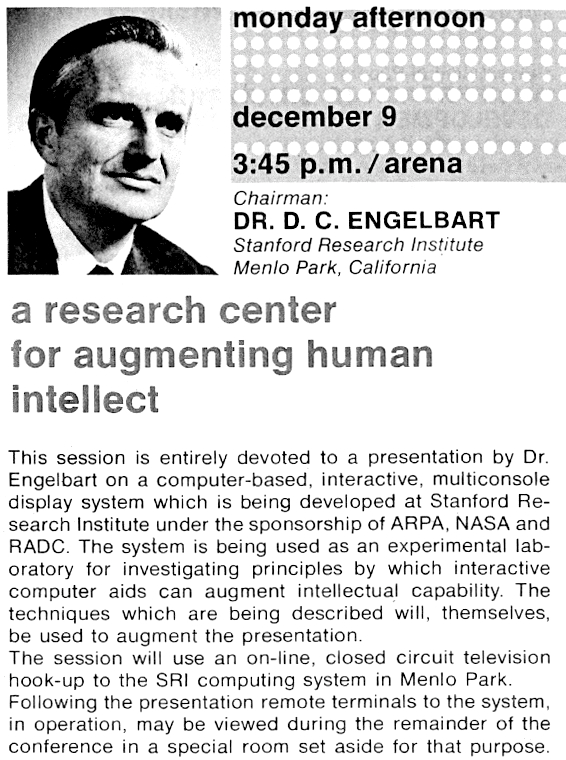
\includegraphics[scale=0.25]{images/images_probert/PRobertV3-img1.jpg}
 \caption*{Annonce de la démonstration de D. Engelbart en 1968}
\end{figure}


On y voit en effet Douglas Engelbart montrer son système tout en l'utilisant. La «~démo~», en ce sens, est cohérente
intellectuellement et pratiquement avec la philosophie du
\textit{bootstrapping}, car elle offre une vue de ce que peut ce dispositif à
travers le dispositif lui-même. Ce n'est pas un discours sur ce qu'il
est possible de faire avec cet outil, c'est une mise en pratique devant
les participants à une manifestation professionnelle de ce qu'il est
possible de faire (à distance d'ailleurs, puisque si les outils
d'interface --~dont la souris~-- sont à San Francisco, l'ordinateur est à
Stanford). Autrement dit, Douglas Engelbart prend le \textit{risque} de
faire cette «~démo~» en direct et inaugure ainsi le genre\footnote{La
«~démo~» est en effet un lieu qui donne à voir la technique à la fois
dans son dispositif (que l'on fait fonctionner) et dans un discours
pratique qui explique comment cela fonctionne : ce geste de D.~Engelbart, 
invente ainsi une mise en scène de l'informatique qui
est devenu une pratique récurrente dans le milieu.}. Mais ce risque,
comme l'effort d'apprentissage, ne font-ils pas partie intégrante d'une
certaine manière de penser et de pratiquer le \textit{bootstrapping} qui est
intrinsèquement innovante ? 

La démo est intéressante par sa mise en scène. Car le
dispositif adopté permet de voir à travers l'écran sur lequel les
instructions et les données qu'introduit Douglas Engelbart
s'inscrivent. Nous sommes de l'autre coté du miroir. Nous voyons ainsi
Douglas Engelbart parler et nous le voyons écrire, bref, nous le voyons
faire la démo comme les gens dans la salle l'ont vue\footnote{Comme le
souligne Engelbart lui-même : «~I saw the same image on my workstation
screen there as was projected for the audience to see~»\footnote{\cite[p.~140]{bardinibootstrapping2001}}.}. Parfois nous avons une vue globale qui présente le système
technique : écran et plateau disposés devant Douglas Engelbart avec les
trois outils d'interface que sont le \textit{Chord Keyset}, le clavier et la
souris. Cette «~démo~» montre comment un homme, armé de ces trois
outils peut créer des \textit{statements} et jouer avec eux ; comment il
peut les manipuler : les créer, les déplacer, les multiplier, les
trier, les classer etc. Bref, pour la première fois on peut assister au
prélude de ce qui va devenir ultérieurement notre quotidien, ce travail
avec et sur des éléments, des données textuelles, chiffrées ou
graphiques. Certes, Douglas Engelbart s'est entraîné et pratique-t-il
l'exercice avec une certaine aisance, mais à un moment ou tout ce qui
est devenu évident pour nous ne l'était pas, même pour lui (il lui
arrive de se tromper).

Ne regardons pas cette «~démo~» avec nos yeux, notre cerveau et nos mains
d'aujourd'hui. Astreignons-nous à la regarder avec les yeux de celui
qui, à l'époque, utilisait une tout autre informatique. Cette évidence,
qui est la nôtre, parce que nous reconnaissons là ce que nous avons
appris à faire depuis, est tout simplement sidérant, radicalement
nouveau (sauf pour une minorité extrême de chercheurs).
Regarder cette «~démo~» c'est remonter à ce moment de l'orée de la
convivialité qui n'est encore en rien conviviale parce que beaucoup
trop nouvelle. Quand bien même on éprouve inévitablement le sentiment
qu'il y a là quelque chose qui change considérablement le rapport à
l'ordinateur, rien ne dit encore que cette manière de dialoguer avec
lui va devenir dominante. Elle n'est évidente à nos yeux qu'à oublier
les apprentissages que nous avons tellement intégrés qu'ils nous
habitent et se font oublier comme tels. Une part de la convivialité
s'invente là, mais elle ne le sait pas (ni même ses inventeurs peut-être) et pourtant elle reste à inventer en tant que telle. C'est ce à
quoi va travailler Alan Kay au Xerox Parc.


\subsection*{1.3~~~Torsion : A. Kay, la convivialité comme \textit{a priori}}
\phantomsection
\addcontentsline{toc}{subsection}{1.3 Torsion : A. Kay, la convivialité comme \textit{a priori}}

Alan Kay n'a jamais directement travaillé avec Douglas Engelbart. Mais à partir de 1971, une partie de l'équipe du laboratoire de Douglas Engelbart, l'ARC
(l'Augmentation Research Center) au SRI (Stanford Research Institute), 
rejoint le Palo Alto Research Center de Xerox, grand lieu de l'innovation technologique en matière
informatique des années 1970. Ce fut le cas de B. English, le co-inventeur de la
souris.

Alan Kay connait bien les travaux de Douglas Engelbart et de son
équipe. Suffisamment pour que Douglas Engelbart se sente quelque peu
plagié. En effet, souligne-t-il : «~they take parts of the architecture,
they take the mouse, they take the idea of the windows, all of that,
but the rest of NLS they just rejected~» \footnote{\cite[p.~154]{bardinibootstrapping2001}.}. Ce qui est
resté sur le bord de la route, c'est justement le \textit{boostrapping}, la
co-évolution par l'apprentissage réciproque : autrement dit on a
conservé le \textit{hard} et le \textit{soft} mais pas la philosophie qui allait avec.
Et, d'une certaine manière, aux yeux de Douglas Engelbart, on a tout
changé. Ce n'est pas tant que les mêmes outils, plongés dans une
approche différente auraient donné de nouveaux outils eux-mêmes
différents. C'est que ces outils proposaient des propriétés dont
l'expression va se trouver transformée par le changement de
philosophie. Car ces propriétés étaient en quelque sorte canalisées
(certains diraient bridées) par le système NLS alors qu'elles vont
exploser si l'on peut dire hors de ses contraintes. De facilitateurs
(les fenêtres comme la souris par exemple) au service de la gestion
d'un outil de gestion de la complexité qui restait lui-même globalement
plutôt complexe et requérait ainsi un apprentissage, ils deviennent des
outils de la convivialité qui s'autonomisent en quelque sorte et
deviennent ce autour de quoi le reste doit tourner, ils deviennent une
fin en soi.

Car la philosophie de Kay est radicalement différente de celle de
Douglas Engelbart. Le premier utilisateur auquel il pense pour son
Dynabook\footnote{«~Several years ago, we crystallized our dreams into
a design idea for a personal dynamic medium the size of a notebook (the
\textit{Dynabook}) which could be owned by everyone and could have the
power to handle virtually all of its owner's information-related
needs~». \cite{kaypersonal2003}.} n'est en rien un
informaticien de haut niveau. Ce n'est pas un chercheur ou un
professionnel dans une entreprise, mais… un enfant. Le système doit être
manipulable par un enfant, c'est bien pourquoi il doit être intuitif et
convivial. Autrement dit, et quelque peu paradoxalement, la mise en
convivialité doit à la fois tout faire tourner autour de ses outils (en
amont, lors de la conception) afin qu'ils se fassent le plus oublier
lors de l'usage de la machine. Car cet usage doit être transparent au
possible et l'apprentissage tout aussi indolore. C'est à dire se faire
oublier comme apprentissage. Nous sommes à des années lumières d'un
processus qui reposait, lui, sur l'effort. Dès lors les outils qui
visaient dans ce cadre à, non pas éliminer l'effort, mais lui permettre
d'aller plus loin dans son efficacité, non pas à l'éradiquer, mais
seulement à le déplacer pour encore mieux gérer la complexité,
deviennent des arguments au service de la valeur centrale de la
convivialité. 

L'étape ultérieure, car la figure de l'enfant ne passe pas forcément
facilement en ce début des années 1970, même chez Xerox, va choisir un
référent certes moins radical, mais néanmoins encore bien naïf ou à
tout le moins candide, une secrétaire, Sally, une cinquantaine bien
avancée, précisaient Tim Mott et Larry Tesler\footnote{\cite[p.~162]{bardinibootstrapping2001}. Larry Tesler,
chercheur au PARC, passera ensuite chez Apple, emportant avec lui ses
compétences dans le \textit{drag-and-drop} et sa connaissance du nouveau
modèle de la souris qui ne fonctionne plus avec des roues (modèle des
années 1960 de D. Engelbart et B. English) mais avec une boule (modèle
des années 1970 de Xerox).}. Une secrétaire et non un
technicien ou un ingénieur. Une secrétaire au service de la gestion
d'une entreprise et dont le travail est un travail de fabrication et de
manipulation de documents (lettres, factures, etc.). N'oublions pas que
Xerox se pense d'abord comme une entreprise de services documentaires,
une \textit{document company}. L'informatique n'est pas une fin en soi,
c'est un outil au service de l'efficacité de la création et de la
manipulation du document de demain. C'est pourquoi la
métaphore du bureau (elle-même proposée par A. Kay) va s'imposer,
sur la base des éléments (fenêtres, dossiers etc.) fournis par les
travaux pionniers de l'ARC ; une métaphore explorée concrètement à
l'aide de l'interface de la souris/pointeur.

Bref, on l'aura compris, la convivialité n'est pas native, elle émerge
d'une torsion des outils au service d'une logique qui vise à faciliter
le travail d'augmentation de l'intelligence (comme outil de gestion de
la complexité) au bénéfice d'une logique qui travaille à réduire
l'effort afin de rendre l'outil le plus «~transparent~»\footnote{Les
couches d'interface graphique qui séparent l'utilisateur du code
peuvent soit être vues comme un allègement parce qu'elles évitent à cet
utilisateur d'investir dans la connaissance et la manipulation du code,
soit comme une barrière puisqu'elles l'éloignent d'une «~vraie~»
maîtrise de l'informatique qui ne peut passer que par celle du code.}
 possible pour qu'il soit utilisable par le plus grand nombre
le plus aisément possible. Ce qui n'est jouable qu'en maximisant le
potentiel intuitif et convivial des outils de base inventés par
l'équipe de Douglas Engelbart (potentiel qui était maîtrisé par les
contraintes du système). Une maximisation qui ne se fait plus au
service du déplacement de l'effort afin de maximiser la gestion de la
complexité, mais au bénéfice d'une convivialité qui veut éviter au
maximum l'effort et limiter au minimum le coût d'apprentissage. 

NLS était un système de travail collaboratif. Il possédait donc des
fonctions de communication et notamment l'une des premières
fonctionnalités d'\textit{e-mail}. Lorsque l'ARC accueille le Network
Information Center d'Arpanet (en toute fin des années 1960), Douglas
Engelbart envisageait que la communauté Arpanet devienne le prochain
lieu de développement de NLS et de la logique du \textit{bootstrapping}. Or,
malgré cette situation carrefour, ce n'est pas la technologie NLS qui
l'emporta, et ses solutions toujours un peu plus
sophistiquées/compliquées, mais l'\textit{e-mail} mis au point par Ray Tomlinson
à BBN en juillet 1970\ldots

\section*{2.~~~La modélisation, la résolution de problèmes et le réseau}
\phantomsection
\addcontentsline{toc}{section}{2. La modélisation, la résolution de problèmes et le réseau}


On présente volontiers la pensée de JCR. Licklider comme largement
orientée par la question de la communication. Elle est certes
centrale\footnote{Je l'ai moi-même souligné dans \cite{robertjcr2011}.}, mais il ne faudrait pas qu'elle en vienne à masquer une autre
dimension tout aussi fondamentale de sa réflexion, celle des modèles
et de la modélisation. Une modélisation dont on retrouve de solides
échos même dans les articles sur la communication et la symbiose. Mais
surtout une modélisation dont la présentation sera beaucoup plus
poussée dans ce qu'il appelle son «~\textit{pro-cognitive system}~» (susceptible
de constituer la bibliothèque du futur) et ses travaux des années 1970
sur une informatique modulaire. On a retenu surtout le réseau --~lui-même
plutôt dépendant de l'armée dans les années 1970, alors que JCR.
Licklider le voyait irriguer l'ensemble de la société~--, tout en oubliant que même la communication chez Licklider est d'abord une question de modélisation des représentations.

La modélisation ou la question des modèles\footnote{Car la question des
modèles renvoie aussi bien à une modélisation plutôt «~dure~» (Cf.
l'article de 1962 et le livre de 1965) qu'à une modélisation plutôt
«~molle~» (de l'échange de modèles entre esprits).} intervient en
quelque sorte dans la vision de Licklider comme l'apprentissage
chez Douglas Engelbart. De même que l'apprentissage ne renie pas les
logiques de facilitation mais empêche leur autonomisation dans une
logique de pure convivialité, de même la modélisation ne renie pas
celle de la communication (homme-machine et/ou réseautique) mais
l'empêche de devenir une pure communication, un pur lien qui pourrait
s'affranchir de la logique de la modélisation. Comme le souligne R. Fano, 

\begin{quote}
He was interested in almost any aspect of human cognitive
activities. While he became a knowledgeable and skillful programmer,
his focus remained on the cognitive aspects of computer usage. He was
fascinated by computers, because he understood in a deep way their
potential to help people in a broad spectrum of activities by extending
and amplifying their intellectual power, by improving the effectiveness
of their communication and collaboration, and last but not least, by
freeing them from the drudgery of clerical operations, to which he was
particularly allergic.\footnote{\cite[p.~20]{fanojoseph1998}.}
\end{quote}

 Toujours, la
dimension cognitive de résolution de problèmes et d'apprentissage l'a intéressé. Or, ces trois dimensions, à ses yeux, passent par la
modélisation. La communication elle-même, dans un tel schéma ne peut
être autonome, elle est inévitablement liée à la question des modèles
qui, à son tour, ne doit pas plus prétendre à l'autonomie ou devenir
une fin en soi, car l'une comme l'autre doivent être au service de la
résolution de problème.




\subsection*{2.1~~~«~On line man-computer communication~»\protect\footnote{Titre de l'article de JC. Licklider de 1962.}}
\phantomsection
\addcontentsline{toc}{subsection}{2.1 «~On line man-computer communication~»}


Ce qui focalise l'attention de JCR. Licklider c'est le \textit{problem-solving}, la résolution de problème. Celle-ci tient en
quelque sorte dans sa vision une place équivalente à celle de la
complexité dans celle de Douglas Engelbart.


\subsubsection*{2.1.1~~~«~Complementation~» et symbiose}
\phantomsection
\addcontentsline{toc}{subsubsection}{2.1.1 «~Complementation~» et symbiose}


La résolution de problemes passe chez Licklider par ce qu'il appelle
une \textit{complementation} entre l'ordinateur et l'homme. Nous sommes en
1962, c'est pratiquement nouveau et intellectuellement rarement
revendiqué comme tel, sauf par Licklider lui-même dans son article de
1960 sur la symbiose. C'est pourquoi il écrit :

\begin{quote}
«~The fundamental aim in designing a man-computer symbiosis is to exploit the complementation that exists between human capabilities and present computer capabilities :
\begin{enumerate}[(a)]
\item To select goals and criteria -- human;
\item To formulate questions and hypotheses -- human;
\item To select approaches -- human;
\item To detect relevance -- human;
\item To recognize patterns and objects -- human;
\item To handle unforseen and low probability exigencies -- human;
\item To store large quantities of information -- human and computer; with high precision -- computer;
\item To retrieve information rapidly -- human and computer; with high precision -- computer;
\item To calculate rapidly and accurately -- computer;
j. To build up progressively a repertoire of procedures without suffering loss due to interference or lack of use -- computer.\footnote{\cite[p.~114]{lickliderline1962}.}
\end{enumerate}
\end{quote}


Est-ce pour rassurer ? Mais une majorité des capacités listées relève de
l'humain en propre (6 sur 10). Deux sont partagées par l'homme et la
machine, à la précision près, ce qui signifie que cette dernière va
l'emporter à terme. Enfin, deux renvoient exclusivement à l'ordinateur.
Toute la question, que n'aborde pas Licklider, n'est-elle pas de savoir si
l'ordinateur va remonter progressivement (puisqu'il parle
de «~\textit{present} computer capabilities~») la liste et laisser la
portion congrue à l'homme, dans une relation moins symbiotique que de
domination ? Une domination qui ne serait pas seulement technique parce
qu'elle aurait des conséquences directes sur la résolution de problèmes
d'organisation socio-politique.

Cette symbiose va s'appliquer aux champs suivants : les mathématiques,
l'informatique, les \textit{war-} et \textit{management gaming},
l'éducation\footnote{Il ajoute également ce qu'il appelle les
\textit{semi-automatic laboratories}, sans expliquer de quoi il s'agit
précisément.}, il ajoute que «~In the planning and design of systems of
many kinds, digital simulation is recognized as a valuable technique~»\footnote{\cite[p.~114]{lickliderline1962}.}. Bref, un univers de résolution de problèmes, pratiques et
conceptuels qui passe le plus souvent par des opérations de
modélisation. 





\subsubsection*{2.1.2~~~Trois applications}
\phantomsection
\addcontentsline{toc}{subsubsection}{2.1.2 Trois applications}



L'article présente ensuite trois applications dans lesquelles
l'articulation entre homme et machine à la fois exige et permet
d'améliorer la modélisation des activités. 





\paragraph{La modélisation des échanges de communication dans l'enseignement.} Modéliser la relation homme/machine permet d'élaborer des systèmes
d'aide à l'enseignement des langues et de l'apprentissage des
mathématiques notamment. 

\paragraph{La simulation hospitalière, le co-planner.} Ce qu'il appelle un co-planner est un dispositif qui articule la
technique (la machine), les données et les programmes qui permettent de
les «~mouliner~».

Encore une fois Licklider fait bien attention à éviter la critique
d'une machine qui remplacerait l'homme : si elle simule, c'est pour
aider la prise de décision et non s'y substituer. C'est pourquoi «~the
computer, parts of the system are not intended, we should emphasize, to
calculate optimal plans or designs; they are intended to provide
memory, manipulative, computing, and display functions in such a way
that they can be integrated with the more intuitive functions supplied
by the human parts of the system.~»\footnote{\cite[p.~118]{lickliderline1962}.}


\paragraph{Visualizing the operation of computer programs.} Enfin, Licklider envisage d'appliquer la démarche de résolution de
problèmes/modélisation à l'informatique elle-même : «~the conclusion,
therefore, is that it might be interesting to experiment with programs
that display various aspects of the internal operation of the running
computer~»\footnote{\cite[p.~119]{lickliderline1962}.}.Cette boucle récursive, l'auteur la compare
volontiers à une «~introspection~», mais ce retour n'est-il pas
moins une conscience qu'un simple outil de contrôle ?


En conclusion, il revient, mais cette fois sous la forme d'une métaphore
(celle de l'œuf et de la poule) sur son idée d'une symbiose. En effet,
écrit-il, «~it appears that the development of effective human
cooperation and the development of man-computer symbiosis are
{\textquotedbl}chicken-and-egg{\textquotedbl} problems. It will take
unusual human teamwork to set up a truly workable man-computer
partnership, and it will take mancomputer partnerships to engender and
facilitate the human cooperation. For that reason, the main tasks of
the first time-sharing computer system with many remote stations may
well be in the areas of language and procedure development.~»\footnote{\cite[p.~119]{lickliderline1962}.}


S'il s'agit, dans cet article, d'améliorer la communication
homme/machine (H/M) réseautique ce n'est pas contre ou au détriment de
la démarche rationnelle/scientifique. Au contraire, Licklider veut
améliorer la capacité de résolution de problème de l'homme en société.
Autrement dit, améliorer l'interface H/M c'est améliorer cette aptitude
en croisant les capacités de l'homme et de la machine et en augmentant
la vitesse d'exécution des opérations. C'est aussi rendre dynamique les
opérations de simulation. Bref, il entrecroise communication et
modélisation, en ce sens que la communication (facilité d'utilisation
et ce, à distance) est au service de la modélisation comme la
modélisation (dynamique) est au service de la communication, tout en
gardant à l'esprit que les deux sont au service de la résolution de
problème et d'aide à la décision. 

\subsection*{2.2~~~Le \textit{procognitive system}}
\phantomsection
\addcontentsline{toc}{subsection}{2.2 Le \textit{procognitive system}}

Au début des années 1960 (de 1960 à 1962) JCR. Licklider, alors chez BBN
(Bolt Beranek et Newman\footnote{ Une des sociétés des plus dynamiques
en matière d'innovation informatique et de réseaux des années 1960.}),
est chargé d'une étude commanditée par le Council on Library
Resources (une organisation crée par la Ford Foundation en 1956).
Cette étude vise à définir ce que sera la bibliothèque du futur,
celle des années 2000, dit-il\footnote{\cite{lickliderlibraries1965}.}. Il souligne que la
science des bibliothèques de l'époque n'offre ni concepts ni système
qui serait efficace ou \textit{desirable} (souhaitable en français ou moins
littéralement «~que l'on aurait envie de promouvoir~») : constat plutôt
négatif. Ce sera l'occasion de revenir sur les outils du savoir et
d'accumulation du savoir développés jusque là --~notamment sur la
bibliothèque et le livre comme outils de
modélisation/présentation/diffusion de la connaissance. Il présente un
modèle simplifié de leurs propriétés essentielles, dont assez
paradoxalement il souligne les limites (ce qui les disqualifie) tout
en conservant une large part des aptitudes acquises de modélisation des
connaissances. Il en vient, bien évidemment, à présenter un système
informatisé qu'il nomme un \textit{pro-cognitive system} pour en souligner
les qualités dynamiques.




\subsubsection*{2.2.1~~~Page, livre et bibliothèque}
\phantomsection
\addcontentsline{toc}{subsubsection}{2.2.1 Page, livre et bibliothèque}



Ce qui intéresse Licklider ce n'est ni le fait que l'information ou
la connaissance soit imprimées sur papier ni même les mots et les
phrases, mais «~the facts, concepts, principles, and ideas that lie
behind the visible and tangible aspects of documents~»\footnote{\cite[p.~2]{lickliderlibraries1965}.}. Ce qu'il
appelle une \textit{transformable information}, c'est-à-dire une information
que l'on peut transporter d'un support l'autre sans déperdition, ou
avec une déperdition/dégradation minimale. Tout ce qui relève de l'art
s'y prête particulièrement mal, car même une reproduction est une
transformation. Même la littérature y perd beaucoup, ce n'est
véritablement valable que pour les activités scientifiques, techniques,
l'histoire, la médecine, le droit et la gestion (des entreprises et de
l'état).


Selon lui les hommes pensent en suivant des schèmes (\textit{schemata}), qui
s'articulent en trois niveaux : le système, les subsystèmes et les
composants. L'innovation doit se faire en réutilisant et modifiant le
niveau des composants. Or, dans le domaine de la bibliothèque : le
système c'est la bibliothèque, les subsystèmes, les livres et les
composantes, les pages. 


D'ailleurs dans ces trois niveaux Licklider considère que la page
est un bon outil d'affichage («~as a medium for display of information,
the printed page is superb~»\footnote{\cite[p.~4]{lickliderlibraries1965}.}), alors que le livre est volumineux
(\textit{bulky}) et lourd (\textit{heavy}) ; bref, «~books are not very good display
devices. In fulfilling the storage function, they are only fair. With
respect to retrievability they are poor~»\footnote{\cite[p.~5]{lickliderlibraries1965}.}. La bibliothèque, qui
regroupe des livres, ne peut être un outil satisfaisant : «~if books are
intrinsically less than satisfactory for the storage, organization,
retrieval, and display of information, then librairies of books are
bound to be less than satisfactory also.~»\footnote{\cite[p.~5]{lickliderlibraries1965}.}


Livres et bibliothèques sont d'autant moins performants qu'ils ne
correspondent pas du tout à ce qu'est, aux yeux de  Licklider,
l'interaction avec ce qu'il appelle le \textit{body of knowledge} :
«~conceived of as a dynamic process involving repeated examinations and
intercomparisons of very small and scattered [dispersées] parts~». Cette
vision est singulièrement proche de la logique du fragment qui domine
aujourd'hui sur internet. Il reproche même à la page imprimée sa
passivité~(ce qui est oublier la dynamique de l'index et de la note de
bas de page voire de l'encadré).


Il en va selon lui de deux difficultés : celle de séparer l'information
de la page elle-même et l'absence de ce qu'il appelle des \textit{active
processors}. C'est pourquoi il veut substituer (il emploie le verbe \textit{to
substitute}) au livre un dispositif qui : transmette/diffuse
l'information sans transport matériel et qui, non seulement présente
l'information aux gens, mais la traite aussi pour eux. Ce substitut se
composera d'une conjugaison de bibliothèque et d'ordinateur. Il
qualifie un tel dispositif de \textit{procognitive system}\footnote{\cite[p.~5]{lickliderlibraries1965}.}, il précise
en note : «~the system in which we are interested are broader than
present day librairies ; the system will extend farther into the
process of generating, organizing and using knowledge~».


Il rejette la page comme outil de stockage de l'information à long terme
mais pas à court terme. D'ailleurs il conserve un certains nombre de
\textit{schèmes} hérités de la page imprimée :

\begin{itemize}
\item La hiérarchie de segments de textes (caractère, mot, paragraphe,
chapitre etc..),
\item Les concepts d'information textuelle, tabulaire, graphique et
picturale/imagière,
\item Des concepts comme ceux d'auteur, d'abstracts, note de bas de page
et liste de références,
\item Des concepts comme article original, compte rendu, note, lettre,
journal et livre («~in the sense of classes of information, not
physical carriers of information~»),
\item Des concepts comme catalogue, index, descripteur et thésaurus.
\end{itemize}



Paradoxalement, au final, il ne rejette pas grand-chose du monde ancien
du livre et des bibliothèques, si ce n'est leur concrétisation
elle-même\ldots mais n'est-ce pas parce qu'il veut introduire un nouveau
support, l'ordinateur ? Nous allons voir cependant que les choses sont
un peu plus subtiles.




\subsubsection*{2.2.2~~~Pertinence de l'informatique}
\phantomsection
\addcontentsline{toc}{subsubsection}{2.2.2 Pertinence de l'informatique}



Si il récuse (partiellement) le vieux monde de la bibliothèque et du
livre, il rejette également une conception déjà dépassée à ses yeux de
l'informatique. Il ne veut plus d'une informatique de données, de
programmes, de cartes perforées, que l'on traite dans un centre
informatique et qui ne peut être l'outil de concrétisation de son
\textit{procognitive system}. Il lui faut une autre informatique qui repose
sur les éléments suivants :

\begin{itemize}
\item Random acces memory,
\item Content adressable memory,
\item Parallel processing,
\item CRT displays and light pens,
\item Procedures, subroutines and related components of computer
programs,
\item Hierarchical and recursive program structures,
\item List structures,
\item Procedure-oriented and problem-oriented languages,
\item Xerographics output units,
\item Time-sharing computer systems with remote stations,
\end{itemize}



La philosophie de sa démarche réside toute entière dans cette idée :
«~what is of value for our purpose is not, for example, the
oscilloscope or the light pen. It is the schema in which a man sits at
a desk, writes or draws on a surface with a stylus, and thereby
communicates to a programmed information processor with a large
memory~». Ce n'est, pas plus qu'avec la bibliothèque et le livre, la
concrétisation qui compte, c'est le concept, le schéma fonctionnel du
dispositif, qui est fondamentalement un dispositif d'écriture-lecture
et de communication (questions-réponses immédiates) avec l'ordinateur,
que ce soit à travers les techniques de l'époque, dont Licklider
connaît à la fois le potentiel et les limites\ldots ou celles de demain
(d'aujourd'hui par exemple) ! C'est pourquoi il souligne qu'il est
«~important to recognize that our progress, must for a time, be largely
conceptual~».


\subsubsection*{2.2.3~~~The procognitive system}
\phantomsection
\addcontentsline{toc}{subsubsection}{2.2.3 The procognitive system}

JCR Licklider part du principe que c'est le système entre l'ordinateur,
l'homme et ce qu'il appelle le \textit{body of knowledge} qui doit être pris
en compte. Pas l'une ou deux seulement des trois composantes. On ne
doit pas non plus reconduire l'approche traditionnelle qui sépare
certaines fonctions allouées à l'homme et d'autres dévolues à la
machine. Il faut tisser les deux ensemble nous dit  Licklider (c'est
lui qui emploie la métaphore de la couverture\footnote{\cite[p.~91]{lickliderlibraries1965}.}). Il
pousse ainsi un peu plus loin encore le programme de l'article de 1962
qui raisonnait, rappelons-le, en termes de «~compensation~».




Son \textit{procognitive system} requiert un médium physique, des langages, et
une capacité d'adaptation, voire d'auto-organisation. Je vais me
focaliser sur le premier point. Licklider préfère le terme
\textit{intermedium} à celui d'interface qui, selon lui, renvoie à la notion
de surface de séparation justement. \textit{Intermedium} est censé dire le lien,
la relation (en écho avec sa philosophie de la symbiose), et être la
base d'un véritable \textit{personal documentation system}.


Les prérequis du système sont les suivants :

\begin{itemize}
\item Un moniteur/écran couleur ou NB («~each element of the display
should be selectively erasable by the computer program, and also either
directly by the operator~»).
\item Il doit permettre d'effectuer des «~hard copy~», des copies
permamentes.
\item Il doit permettre de faire des dessins et des graphiques, grâce à
un stylet («~if the stylus is connected by a wire to console, the wire
should be very light and flexible and should not constrain the
manipulation of the stylus~» --~ce qui nous semble une \textit{évidence}
aujourd'hui et ne l'est pas à l'époque),
\item Le dispositif doit également être fiable et économiquement viable.
\item Il doit aussi posséder une interface d'écriture, un clavier ; Licklider souligne que dès lors qu'un clavier est connecté à un
ordinateur il n'y a plus de raison pour que ce qui est tapé soit
immédiatement imprimé sur une feuille de papier, il peut l'être, mais
va d'abord être affiché sur l'écran --~là encore, ce qui nous parait une
\textit{évidence} aujourd'hui mérite une remarque précise de l'auteur à
l'époque. 
\end{itemize}

Licklider prévoit que son \textit{procognitive system} ne doit pas faire
l'objet que d'une seule utilisation individuelle. C'est aussi un outil
de travail en groupe, un outil de travail collaboratif (pensons à NLS
d'Englebart). Il envisage deux solutions :

\begin{itemize}
\item Des consoles reliées entre elles selon des techniques qu'il
renvoie explicitement au téléphone et à la TV (alors que ses idées par
ailleurs mèneront au développement d'une logique de réseau purement
informaticienne).
\item Un dispositif de projection sur grand écran, avec un dérivé du
\textit{light pen} pour la communication entre les membres du groupe et la
machine et un puissant système de zoom (Power-point et Google maps tout
ensemble avant la lettre ?).
\end{itemize}


\subsection*{2.3~~~La fin des années 1960}
\phantomsection
\addcontentsline{toc}{subsection}{2.3 La fin des années 1960}

Qu'est-ce donc que «~communiquer~» pour notre auteur dans son article de
1968 «~Computer as a Communication Device~»~? Communiquer, c'est échanger des
modèles informationnels à propos de quelque chose. Des modèles qui
doivent être sanctionnés par la société. Autrement dit la communication
est définie par Licklider comme une opération de \textit{cooperative modeling}. Opération soutenue par des moyens d'\textit{externalization} : «~Even such a simple externalized model as a flow diagram or an outline --~because it can be seen by all the communicators~-- serves as a focus for
discussion. It changes the nature of communication.~»\footnote{\cite[p.~22-23]{licklidercomputer1968}.}


L'ordinateur ne doit pas être utilisé seulement comme outil
d'automatisation de tâches. C'est ce à quoi aboutit Licklider après
avoir pris connaissance des travaux de D. Engelbart sur les interfaces
et l'interaction (le système souris-pointeur par exemple). 

\begin{quote}
We can say
with genuine and strong conviction that a particular form of digital
computer organization, with its programs and its data, constitutes the
dynamic, moldable medium that can revolutionize the art of modeling,
and that in so doing can improve the effectiveness of communication
among people so much as perhaps to revolutionize that also.\footnote{\cite[p.~27]{licklidercomputer1968}.}
\end{quote}

Soulignons que l'ordinateur est vu, dès cette époque comme un \textit{medium}
par Licklider, ce qui est pour le moins nouveau. Et ce médium est à la
fois modélisé/modélisant et pensé comme ce qui va «~révolutionner~»
l'exercice même de la modélisation. Or, cette modélisation ne s'oppose
pas à la communication qui, pour le psychologue qu'est avant toute
chose JCR. Licklider est échange de modèles de représentations. C'est
pourquoi il revient encore une fois sur l'idée que «~creative,
interactive communication requires a plastic or modable medium that can
be modelled, a dynamic medium in which premises will flow into
consequences, and above all a common medium that can be contributed to
and experimented with by all~[\ldots]~»\footnote{\cite[p.~22]{licklidercomputer1968}.}


Toujours en cette fin des années 1960, Licklider avait à l'esprit un ordinateur qui
pourrait être utilisé par des chercheurs non spécialisés en
informatique, avec un minimum de programmation. Or, ce qui intéresse un
chercheur d'une autre discipline selon Licklider, c'est de pouvoir
utiliser l'ordinateur comme un outil de modélisation. Un outil de
modélisation avec lequel on peut interagir directement grâce à un
dispositif d'interface graphique. Le chercheur aurait à sa disposition
(et/ou créerait) une bibliothèque de modules logiciels qu'il pourrait
ensuite utiliser comme des outils au service de ses besoins de
modélisation. Chaque module serait indexé pour pouvoir être facilement
réutilisé. Vision puissante, mais fort difficile à mettre en œuvre à
l'époque. Licklider s'est beaucoup investi personnellement dans
cette démarche entre 1969 et 1974 sur un financement IPTO, et sa
bibliothèque a atteint les 2000 modules\ldots Cependant, l'ARPA avait pour
objectif de financer des projets dans leur phase de lancement, c'est à dire cinq années.
 Dès lors, après 1974, Licklider
se retrouva sans financement\ldots et le projet périclita, d'ailleurs il
n'écrivit aucun article ni rapport sur ce projet\ldots on peut y voir plus
qu'une déception.


Aujourd'hui, la prégnance d'Internet --~et plus globalement
celle des réseaux (d'informatique et de télécommunications)~--  est telle que l'on
relit volontiers le travail de Licklider à l'aune de la question de
la communication en oubliant peut être que la pensée de
 Licklider s'adressait autant aux questions de la résolution de
problèmes et de la modélisation. La communication homme/machine et
réseautique n'étant, d'une certaine manière, qu'un outil au service de
leur efficacité. Certes, Licklider a publié un article sur les
réseaux\footnote{\cite{licklidermemorandum1963}.} en 1963 et il a
été le directeur de l'Ipto\ldots mais pendant deux ans seulement (de 1962 à
1964) bien avant le lancement d'ARPANET et alors que son grand projet --~MAC~-- est un projet de \textit{time sharing} ; certes, ses idées, reprises par Robert Taylor et Larry Roberts, ont participé au développement
d'ARPANET, mais les réseaux qu'envisage Licklider relèvent largement
d'une technologie, le \textit{time-sharing}, qu'il promeut dans ses travaux de
1960/1962 et 1968, et qui sera amplement dépassée dès la fin des années
1960. ARPANET, en ce sens, n'est pas une application des idées de Licklider. C'est pourquoi il n'est pas aberrant de considérer que le
poids rétrospectif que font peser les réseaux en vient à opérer une
\textit{torsion} non négligeable de sa vision de l'ordinateur conçu en premier comme outil de
résolution de problèmes/modélisation. Une torsion qui oublie que cette
logique met la communication à son service (au moins autant que
l'inverse) et qu'elle leste le projet de Licklider d'un poids (celui d'investissements lourds), d'un sérieux (dans le management des projets) qui participent certes à alléger les
apprentissages mais, là encore pour aller plus loin et plus vite, c'est-à-dire sans les renier.

\section*{Conclusion}
\phantomsection
\addcontentsline{toc}{section}{Conclusion}

En définitive, l'histoire de l'informatique des années 1970 correspond à
une torsion des visions de D. Engelbart et JCR. Licklider (on
peut aussi considérer que la déformation de ces visions s'offre comme
un outil de lecture/décryptage de cette histoire) qui aboutit à la mise
entre parenthèse de l'apprentissage et de la modélisation au bénéfice
de la convivialité ou de la communication dans le cadre de systèmes
plutôt fermés (d'abord chez Xerox puis avec Apple). On peut alors se
demander si le Libre ne correspond pas à la «~reprise~» (mais sans
forcément assumer une continuité) de la logique de l'apprentissage et
de la modélisation (au sens large). Car s'il est «~libre~» c'est aussi
sur le fond de l'exigence d'un accès difficile qui nécessite un long et
intense apprentissage et d'un fort investissement technique (quand bien
même certains l'oublient parce qu'ils ne le vivent pas comme tel).
Autrement dit, la «~liberté~» technico-sociale appelée de ses vœux par
le mouvement du Libre est en quelque sorte payée par le prix de l'acquisition
d'une compétence technique élevée. Ne buttera-t-elle pas toujours sur
une convivialité et une communication peut être aliénantes, mais
socialement et cognitivement moins coûteuses ? 

\nocite{engelbartaugmenting1962,engelbartresearch2003,foucaultarcheologie1969,lickliderman-computer1960,licklidermemorandum1963,robertmnemotechnologies2010}





\printbibliography[heading=subbibliography]
\end{refsection}

%%%%%%%%%%%%%%%%%%%%%%%%%%%%%%%%%%%%%%%%%%%%%%%%%%%%%%%%%%%%%%%%%%%%%%%%%%%%
%
\part{Contextes économiques}
\phantomsection
%\addcontentsline{toc}{part}{Contextes économiques}
%
%%%%%%%%%%%%%%%%%%%%%%%%%%%%%%%%%%%%%%%%%%%%%%%%%%%%%%%%%%%%%%%%%%%%%%%%%%%%
%--------------------------------------------------------------------
\chapter*{Les modèles économiques du logiciel libre et leur évolution} 
\phantomsection                 
\addcontentsline{toc}{chapter}{Les modèles économiques du logiciel libre et leur évolution \\ \textit{Stéphane Ribas, Patrick Guillaud, Stéphane Ubéda}}
%--------------------------------------------------------------------

\fancyhead[LO]{\small Les modèles économiques du logiciel libre et leur évolution}
\fancyhead[RE]{\small Stéphane \textsc{Ribas}, Patrick \textsc{Guillaud}, Stéphane \textsc{Ubéda}}
%%\setcounter{section}{0}
\begin{refsection}

\begin{flushright}
Stéphane \textsc{Ribas}, \\
Patrick \textsc{Guillaud}, \\
Stéphane \textsc{Ubéda}
\end{flushright}
\vspace{10 mm}

\epigraph{\textit{Un logiciel libre est gratuit une fois qu'il a été payé} \\ François Élie}



Le mouvement du logiciel libre représente actuellement environ six cent
mille projets et plus de cent millions de développeurs. Plus de la
moitié des solutions et des infrastructures installées par les
entreprises dans les cinq ans à venir seront basées sur du logiciel
libre. 2011 a été une année record pour les investissements dans ce
domaine avec une augmentation de 49\% pour atteindre 675 millions de
dollars. Les nouvelles entreprises de logiciel s'appuient de plus en
plus sur le logiciel libre qui leur permet de générer du chiffre
d'affaires avec des modèles économiques adaptés.

Ces chiffres et projections issus d'études récentes réalisées par
Blackduck Software (\textit{6th Annual Future of Open Source Survey})
donnent une idée de l'ampleur du mouvement du libre qui est aujourd'hui
bien installé dans le paysage économique. Ce chapitre apporte des
réponses à la désormais classique question de savoir comment générer du
chiffre d'affaires et des revenus à partir de logiciels qui sont
ouverts et gratuits.

À l'instar du réseau routier dont la fonction première est de faciliter
les déplacements des usagers indépendamment de leurs activités, les
logiciels libres sont indépendants des modèles économiques liés à leur
utilisation. Une conséquence importante est que le mouvement du
logiciel libre offre deux types de retour sur investissement : le
premier répond au modèle de l'édition logicielle
(amortissement des coûts de développement) et l'autre,
moins facile à quantifier, intervient à travers
l'impact sociétal produit, qui peut être
parfois considérable (par exemple Internet).

Dans ce chapitre nous présenterons, en adoptant une perspective
historique, le concept d'\textit{openness} et les
différents modèles économiques associés au logiciel libre : services,
mutualisation, valeur ajoutée, double licence, fondation. Seront
également évoqués des modèles basés sur le matériel, le cloud,
l'assemblage de composants et les terminaux mobiles.
Avant d'aborder ces questions nous rappellerons quelques concepts
clés.

\paragraph{Qu'est-ce qu'un modèle économique ?} Pour en donner une définition très succincte, un modèle économique est
une description des mécanismes de génération de revenus, que ce soit
pour des personnes physiques (artisans, etc.) ou morales (entreprises,
collectivités, etc.). Les modèles économiques sont aussi vieux que la
société : le marchand itinérant qui augmente la valeur perçue de ses
produits en les déplaçant d'un point à un autre, la
place du marché où les commerçants produisent mutuellement de la valeur
en concentrant des produits, donc du choix, dans le temps et dans
l'espace, l'échoppe de quartier qui
offre un point d'approvisionnement stable pour les produits courants,
le travail à façon qui mobilise les compétences spécifiques de
l'artisan, etc. Les modèles économiques rencontrés dans le monde du
logiciel libre sont liés à une gestion de la propriété intellectuelle
spécifique puisque le principe des licences du logiciel libre consiste
en un abandon contrôlé, parfois imposé, des droits patrimoniaux des
auteurs.

\paragraph{La non rivalité et l'openness.}
Le logiciel libre est fondé sur deux principes essentiels : la «~non
rivalité~» et l'\textit{openness}. Un bien est dit «~non rival~»
lorsqu'il qu'il peut être transmis sans dépossession, comme la
connaissance. Les logiciels appartiennent aussi à cette catégorie : on
peut copier et transmettre un logiciel autant de fois que l'on veut
tout en continuant à s'en servir soi-même. Le concept d'ouverture ou
\textit{openness} peut être défini comme l'attitude consistant à
systématiser la diffusion et le partage des biens non rivaux. Ce type
de comportement, dont l'exemple le plus emblématique est celui de la
recherche scientifique, accélère considérablement la production et la
diffusion des connaissances et augmente significativement l'innovation.
La réponse que fournit l'\textit{openness} à la question du mode de
financement s'appelle \textit{écosystème} et nous verrons que les
implications de cette réponse excèdent largement le seul financement du
développement du logiciel.

\paragraph{Le prix, le coût et la valeur perçue.}

Tout modèle économique fait intervenir au moins trois grandeurs
fondamentales. Le prix d'un produit ou d'un service qui est déterminé
par un vendeur en fonction d'un contexte de marché, c'est le prix
«~affiché sur l'étiquette~». Le coût d'un produit ou service qui
correspond à la somme des ressources nécessaires à celui qui le
fabrique ou l'élabore pour le produire ou le fournir. La valeur perçue
d'un produit ou service est l'évaluation par un acteur donné de
l'intérêt que présente pour lui l'acquisition de ce produit ou ce
service. Le prix résulte donc d'une décision, le coût d'une analyse et
la valeur perçue d'une évaluation. Ces trois variables sont relatives,
elles dépendent de chaque acteur et déterminent des indicateurs (ex.
marge ou perte) et des comportements (ex. décision d'achat ou non). La
nature des articulations entre ces trois grandeurs et leur organisation
dans le temps et dans l'espace sont caractéristiques d'un modèle
économique.

\paragraph{Réseau routier, Internet et logiciel libre.}
La fonction d'un réseau routier est de faciliter la circulation, quel
que soit le type des véhicules qui l'empruntent (vélo, voiture, bus,
camion, etc.), et indépendamment de la nature de l'activité (trajet
privé pour se rendre à l'école ou au travail, trajet professionnel,
transport en commun, de fret, etc.). Partant de ce constat on peut
imaginer de modéliser le réseau routier, les véhicules qui l'empruntent
et la nature des déplacements, en une série de «~classes~» d'éléments.
Le réseau routier est une instance d'une classe «~infrastructures~»
contenant toutes sortes de réseaux : le réseau Internet, d'électricité,
réseau ferré, etc. De la même façon on peut considérer une classe
«~types de véhicules routiers~» contenant une collection de dispositifs
adaptés à la circulation sur l'instance «~réseau routier~». Une classe
«~applications~» contiendrait des instances de type «~service de
transport de personnes~», «~déplacement individuel privé~», etc. On
peut envisager une classe «~types de protocoles~» de l'infrastructure
«~Internet~» qui correspondrait à la classe «~type de véhicules~» de
l'infrastructure «~réseau routier~». Il est également possible de
dessiner une séparation entre les classes de niveau inférieur qui
concernent l'infrastructure et celles de niveau supérieur concernant
son utilisation. L'extension de cette analogie au domaine du logiciel
permet de constater que le logiciel libre se situe souvent au niveau
structurel : il est le composant essentiel de l'infrastructure
«~Internet~» (dont la description de ses protocoles, les «~véhicules~»
qui y circulent) et concerne la majeure partie des briques de base des
systèmes d'information constituant le web (GNU/Linux, Apache, MySQL,
PHP, etc.).

Il apparaît que les acteurs qui contribuent aux infrastructures et ceux
qui contribuent aux applications ne sont pas les mêmes. Les premiers
sont généralement des institutions de recherche, des universités dont
l'objectif initial n'est pas de réaliser des profits financiers
immédiats mais de faire progresser les connaissances de manière
collaborative, ouverte et mutualisée en créant des infrastructures à
disposition de la société toute entière et sur lesquelles le secteur
privé peut s'appuyer notamment pour exercer des activités commerciales.
Cette complémentarité des modèles, à laquelle nous devons notamment
Internet, le Web, est d'une remarquable efficacité puisque l'on estime
aujourd'hui à 3~500 %ici cela doit s'écrire 3~500
milliards de dollars le chiffre d'affaires généré
notamment par les 113 millions de sites web actifs sur l'infrastructure
Internet\footnote{\cite{mogleninnovation2012}.}.%%%% ICI REF BIBLIO
 L'évocation de ces chiffres astronomiques est
l'occasion de remarquer qu'une approche financière directe est
extrêmement réductrice car elle est incapable de mesurer d'autres
effets comme les interactions entre personnes ou la formation et la
diffusion des connaissances, ou encore la circulation de l'information,
qui sont pourtant des facteurs clés pour l'innovation. Le parcours
historique qui suit va nous permettre de présenter les moyens qu'ont
trouvés les acteurs du logiciel libre pour générer de la valeur.






\section*{1.~~~Années 1960 et 1970 les débuts de l'informatique, des modèles économiques basés sur le matériel}
\phantomsection
\addcontentsline{toc}{section}{1. Années 1960 et 1970 les débuts de l'informatique, des modèles économiques basés sur le matériel}

Durant les décennies de 1960 et 1970 le marché percevait la valeur de
l'informatique comme étant concentrée dans le
matériel\footnote{Nous indiquerons en note de bas de page le modèle
économique mis en œuvre, précédé de «~ME~». Dans ce cas il
s'agit de la vente d'un ensemble
indissociable constitué d'un équipement matériel et
des logiciels permettant de l'exploiter.}. Les
logiciels constituaient un complément nécessaire permettant de rendre
les ordinateurs utilisables. Les systèmes d'exploitation, destinés à
animer les machines, et les utilitaires, étaient considérés comme
secondaires : leur finalité était de permettre aux constructeurs de
valoriser leur offre matérielle. Les logiciels alors financés par les
constructeurs d'ordinateurs étaient fournis avec les machines. De ce
fait, les programmeurs étaient libres de mutualiser et d'échanger leurs
codes. Ce fut le temps des premiers hackers, le développement logiciel
s'inspirait du modèle de la recherche basé sur
l'ouverture, le partage et la réutilisation. Les
questions liées à l'appartenance, à l'encadrement de
leur utilisation, à leur modification ou leur diffusion
n'étaient pas à l'ordre du jour.
Cette situation a perduré tant que les revenus des constructeurs
d'ordinateurs s'est limité à la vente
d'équipements matériels spécifiques. Cependant, avec
l'évolution et la complexification des machines, les coûts de
développement augmentèrent et les programmes livrés par les
constructeurs dans des versions minimales ne satisfirent plus tous les
utilisateurs. Les grands laboratoires de recherche et les universités
commencèrent alors à développer des logiciels pour mieux répondre à
leurs besoins, enrichissant ainsi l'offre des constructeurs de codes
plus complets, plus performants et qui circulaient librement. Un
exemple emblématique est le système d'exploitation Unix, développé par
les laboratoires Bell à la fin des années soixante et commercialisé à
partir de 1975. Caractérisé par sa portabilité --~il ne dépendait pas
d'un constructeur~-- et par sa structure modulaire, Unix se diffusa
rapidement dans le monde universitaire. L'université de Californie à
Berkeley disposant des codes sources fit évoluer le système en adoptant
un modèle collaboratif de développement qui préfigurait l'organisation
des communautés \textit{open source}. Cette initiative fut à l'origine
de la première distribution Unix, la Berkeley Software Distribution ou
BSD. L'association de BSD et des ordinateurs VAX de Digital Equipement,
souvent mis à disposition des laboratoires universitaires par ce
constructeur, en ont fait le premier système informatique de référence
dans le milieu académique. Un détail d'importance pour la suite fut
l'adjonction par les développeurs de Berkeley du support de TCP/IP dans
BSD, faisant ainsi de chaque ordinateur VAX installé une machine
«~\textit{Internet ready}~» près d'une décennie avant l'adoption
d'Internet par le grand public. Un autre point à noter est la grande
attention portée à la qualité du manuel d'utilisation d'Unix dont le
format standardisé respectait des règles extrêmement strictes. Ce soin
porté à la rédaction du manuel est souvent cité comme l'un des facteurs
clés de succès d'Unix. 

À cette époque Richard Stallman, chercheur au MIT et spécialiste de la
programmation, des langages et des systèmes
d'exploitation, commença à réfléchir à la création
d'une licence garantissant le libre usage des logiciels, la libre
accessibilité de leur code et réservant aux utilisateurs la possibilité
d'étudier, de modifier, d'améliorer et de redistribuer les codes
modifiés. Stallman annonça également son ambition de créer un système
Unix dont tous les composants seraient libres. Plusieurs de ses
collègues soutinrent cette initiative et en 1976 le groupe diffusa le
premier éditeur libre Emacs, puis un an plus tard le gestionnaire de
dépendances Make, suivi d'un débogueur puis d'autres outils. Le groupe
fut rejoint par un nombre croissant de programmeurs à travers le
monde.\footnote{ME : création d'un écosystème.} La
dissémination d'Unix et la standardisation de l'informatique
professionnelle provoqua un foisonnement de petites entreprises
spécialisées dans le développement d'applications spécifiques et
d'édition de logiciels standards. Cela constitua le point de départ du
développement d'un nouveau secteur économique d'autant plus prometteur
que l'évolution rapide de la taille du parc de machines laissait
entrevoir un marché potentiellement gigantesque.

En somme, les modèles économiques des décennies 1960 et 1970 (et un peu
au-delà)~se sont construits autour du système Unix.
C'était le règne du matériel et la période des
architectures client/serveur. La source principale de revenus des
constructeurs informatiques était la vente
d'équipements matériels, le logiciel étant «~offert~»\ldots

\section*{2.~~~Années 1980, l'époque des pionniers du libre}
\phantomsection
\addcontentsline{toc}{section}{2. Années 1980, l'époque des pionniers du libre}

Au début des années 1980 le système d'exploitation Unix
de Bell Labs dominait largement le marché Américain. On dénombrait 400
installations de systèmes Unix dans les universités en 1982 (contre 3
en 1979) et ce chiffre n'a cessé
d'augmenter pendant les décennies 1980 et 1990. La
plupart des étudiants qui travaillaient et développaient sur ce type de
système utilisaient les outils «~libres~» avant de partir travailler en
entreprise où ils trouvaient - ou mettaient en place - les mêmes
environnements.\footnote{ME : l'activité académique
favorise la création d'écosystèmes.} La licence du
système Unix, qui accorde le droit d'utiliser le système, était achetée
à Bell à un prix modeste mais, une fois cette formalité remplie, la
plupart des utilisateurs installait BSD, la distribution universitaire
du système qui rassemblait tous les utilitaires libres. La diffusion de
ces logiciels empruntait un nouveau vecteur : Usenet, un réseau
communautaire d'échange de messages, de programmes, de support, entre
des centaines de programmeurs. Le déploiement d'Usenet, favorisé par le
support de TCP/IP par la plupart des machines sous Unix, généralisa la
diffusion des programmes par voie numérique et en même temps installa
l'idée qu'un logiciel est naturellement et légitimement libre.
L'architecture de Usenet était non centralisée, le réseau diffusant les
contenus de proche en proche sur les réseaux des universités mais
également entre universités. Ce furent les prémices d'Internet. En 1980
à Berkeley une passerelle fut établie entre le réseau ARPANET, qui
reliait l'ensemble des établissements en contrat avec
le Département de la Défense, et Usenet. En 1985 les messages Usenet
adoptèrent le format NNTP qui s'imposa comme le standard de la
transmission de news, ce qu'il est encore aujourd'hui.\footnote{ME :
l'émergence de standards ouverts est un terreau
favorable au développement économique.}

En 1983 la position dominante de AT\&T entraîna le découpage des Bell
Labs en une série de petites compagnies privées autonomes et le système
d'exploitation Unix devint un produit commercial comme un autre. Les
universités furent alors confrontées à un problème inattendu : elles
durent désormais payer leurs licences Unix bien plus cher
qu'auparavant\footnote{Jusque-là les licences étaient gratuites pour
les applications liées à la recherche et très peu coûteuses pour les
usages administratifs.} pour pouvoir utiliser le système. La
réaction des universitaires ne tarda pas et en 1984, Richard Stallman
lança le projet GNU avec l'objectif de développer de manière
collaborative un système d'exploitation équivalent à Unix qui serait
libre, gratuit et modifiable.\footnote{ME : la mutualisation de
l'effort de développement par effet de levier est une
source de croissance pour les entreprises, elle leur permet
d'affecter leurs ressources sur leur cœur de métier.}

Un an plus tard Stallman créa la Free Software Foundation (FSF) afin de
garantir l'ouverture des codes publiés dans le cadre du projet GNU et
les garantir contre le risque d'une appropriation. La FSF énonça les
quatre libertés du logiciel libre : liberté d'exécuter le programme
pour tous les usages, liberté d'étudier le fonctionnement du programme
à travers son code source et de l'adapter, liberté de distribuer des
copies, liberté d'améliorer le programme et de le rediffuser accompagné
de son code source.

Quelques années auparavant IBM avait sous-traité le système
d'exploitation de sa nouvelle gamme de micro-ordinateurs IBM~PC à
Microsoft. Le grand succès de cette machine généra d'importants revenus
pour Microsoft et l'entreprise se lança dans l'écriture d'une couche
d'interface graphique destinée à concurrencer le nouveau produit
d'Apple, le Macintosh, qui était muni d'une interface graphique
fenêtrée avec des icônes et un dispositif de pointage intégré. Les
métiers de ces deux entreprises étaient très différents et ces
dernières ont déployé des stratégies différentes. Apple, qui
amortissait le développement du système d'exploitation de sa machine en
intégrant son coût dans le prix de vente de ses micro-ordinateurs,
suivait le modèle économique historique de l'informatique en
fournissant le système d'exploitation en même temps qu'elle vendait
l'ordinateur, donnant ainsi aux clients l'impression que le logiciel
système était gratuit. Microsoft, qui ne vendait pas de matériel mais
seulement des logiciels qui pouvaient être dupliqués par simple copie,
fut alors confronté à un problème inédit. La stratégie de l'éditeur
consista à passer des accords avec les constructeurs de matériel afin
que son système d'exploitation soit pré-installé sur
les machines commercialisées\footnote{ME : la vente liée est
controversée, voire interdite, mais elle permet de réaliser
d'importants profits.} soumettant l'utilisation des
ces dernières à l'acceptation d'un «~contrat de licence d'utilisateur
final~» (ou CLUF, en anglais «~\textit{end-user license agreement}~»,
EULA). Ce contrat limitait considérablement les droits de l'utilisateur
du système en lui imposant une longue série d'interdictions, notamment
de revendre sa licence, de réinstaller le logiciel sur une autre
machine ou d'en utiliser des copies sur plusieurs machines. Cette
pré-installation généralisée des systèmes d'exploitation de Microsoft
sur les micro-ordinateurs constitua une barrière à l'entrée efficace
qui a longtemps entravé la diffusion de systèmes d'exploitation
alternatifs, ce malgré leur disponibilité (DR-DOS, Concurrent CP/M86,
MultiUsers Dos, FlexOS 286, etc.).

Malgré la protection apportée par la GPL la communauté GNU peinait à
développer le noyau qui lui aurait permis de disposer de son système
d'exploitation libre. Pour autant, cela n'entrava pas
une montée en puissance du développement de logiciels libres, et
notamment des outils, durant toute la décennie. Les méthodes de
développement collectif commencèrent à se formaliser, notamment grâce à
l'arrivée d'Internet qui était de plus en plus utilisé pour échanger
des données dans le milieu du développement logiciel : on apprenait à
travailler à distance, à s'organiser, on développait des outils
collaboratifs. 

En 1988, Digital Equipement Corporation réunit les grands constructeurs
(HP, Bull, IBM, Nixdorf, Siemens, Apollo) autour de l'initiative Open
Software Foundation avec l'objectif d'assurer la standardisation
d'Unix.\footnote{ME : premier modèle à fondation,
rassemblant des concurrents autour d'un projet
commun.}

Cette volonté des principaux acteurs du monde Unix de travailler
ensemble sur un projet de standardisation montre que dans ces grandes
entreprises on considérait unanimement une collaboration entre
concurrents comme étant favorable aux affaires. Après une longue
période pendant laquelle les acteurs tentaient de se distinguer les uns
des autres avec des solutions volontairement différenciées, la
standardisation est apparue comme un atout.\footnote{ME : la
standardisation permet de favoriser l'émergence
d'écosystèmes propices aux affaires.}

IBM décida alors de développer AIX, sa version d'Unix,
et HP la sienne, HP-UX. Au même moment l'IEEE spécifiait le standard
d'API Posix pour tenter de rendre les différentes variantes d'Unix plus
interopérables. On voit apparaître ici une séparation entre des couches
basses (le système d'exploitation avec ses services de
base) pour lesquelles les concurrents n'hésitaient pas à collaborer en
mutualisant leurs efforts, et les couches supérieures (ergonomie,
richesse fonctionnelle, etc.) qui constituaient le lieu de la
concurrence commerciale. Les principes énoncés par la FSF et appliqués
par le projet GNU donnèrent lieu en 1989 à la création de la General
Public Licence ou GNU GPL qui formalisa les droits et devoirs des
créateurs et des utilisateurs du logiciel en défendant
l'idée que l'utilisateur doit pouvoir
contrôler les programmes et non le contraire. Ce recours à la dimension
juridique pour encadrer l'utilisation du logiciel à
travers une licence fut une étape déterminante pour le logiciel libre.

Ainsi la décennie 1980 a vu émerger des solutions alternatives à Unix :
Microsoft Windows et l'IBM PC, le Macintosh
d'Apple et les prémices du logiciel libre (outils
de développement GNU, etc.). Le modèle de vente liée ( CLUF/EULA) et de
vente d'ensembles représentait alors une part
importante du marché. Le logiciel libre en était à ses débuts, la
priorité des développeurs étant le développement de logiciels
d'infrastructure et d'outils (réseau,
\textit{middleware}, bases de données, serveurs web). Les solutions
propriétaires furent progressivement remplacées par des logiciels
libres dans un mouvement partant des infrastructures et orienté vers
les couches applicatives.

\section*{3.~~~Années 1990, naissance de GNU/Linux, du logiciel libre à l'Open Source Initiative (OSI)}
\phantomsection
\addcontentsline{toc}{section}{3. Années 1990, naissance de GNU/Linux, du logiciel libre à l'Open Source Initiative (OSI)}

L'un des évènements marquants du début de la décennie quatre-vingt dix
fut la naissance du World Wide Web, dont Tim Berners Lee, chercheur au
CERN décida de libérer les logiciels :

\begin{quote}
D'abord, il n'est pas
évident que je serais devenu un homme très riche si
j'avais fait breveter une chose ou deux, parce
qu'il y a plein de petits projets hypertexte qui
n'auraient pas décollé dont une bonne partie à cause
de l'existence d'un contrôle central.
Si j'avais été la personne centrale auprès de laquelle
vous auriez dû enregistrer chacun de vos clics, payer pour chacun de
vos clics, ou enregistrer chacune de vos pages web alors
j'aurais eu un business model. Mais aucun business
n'aurait existé. Il n'y aurait pas eu
de web. A la place il y aurait eu plein de gens qui auraient créé plein
de webs incompatibles, ils auraient tenté de contourner mes brevets,
donc ils auraient fait des systèmes qui n'auraient pas
fonctionné de la même façon.\footnote{\cite{berners-leewriting2007}. ME : un
choix doit être fait entre velléités de contrôle et le potentiel de
diffusion d'un projet d'open source.} 
\end{quote}


En février 1992, Linus Torvalds diffusa son noyau Linux sous licence
GPL. Les développeurs affluèrent pour contribuer et dans le courant de
l'année les premières distributions firent leur apparition. C'est à ce
moment que furent créées les premières entreprises privées dont le
modèle économique était basé sur le logiciel libre. La société Cygnus
Solutions présentée comme pionnière en la matière proposa des services
de support des outils de développement GNU. Michael Tiemann, fondateur
de la société, a fait le pari qu'un marché existait désormais en
s'inspirant du GNU Manifesto dans lequel Stallman suggérait que des
activités de consulting et de services autour du logiciel libre
pouvaient tout à fait permettre de gagner sa vie. Stallman partait du
principe que le logiciel à code ouvert engendre un marché de services
d'une qualité bien supérieure pour les clients que l'offre
monopolistique associée aux logiciels propriétaires. Après s'être
convaincu qu'il était possible de proposer des prestations avec une
efficacité de deux à quatre fois supérieure à une prise en charge
interne, et cela pour un coût de deux à quatre fois inférieur, Tiemann
lista quelques questions clés permettant d'évaluer les chances de
succès d'un modèle : 
\begin{itemize}
	\item estimer la valeur qu'il est possible de produire,
	\item vérifier que le modèle passe à l'échelle,
	\item préciser le niveau de problème que l'on est en mesure de traiter,
	\item estimer le rythme d'innovation le projet peut soutenir\footnote{\cite{tiemannhistory2012}.} 
\end{itemize}

Au cours de la décennie 1990, les distributions GNU/Linux continuèrent à
apparaître : la Debian en 1993, puis la Red Hat en 1994\footnote{ME :
édition de distributions de logiciels à valeur ajoutée (installeur,
intégration, cohérence et compatibilité des versions, assurance
juridique, etc.).}. Alors que la diffusion du logiciel libre se limitait
jusque-là à des distributions de GNU/Linux intégrant des utilitaires
système, des logiciels applicatifs apparurent : un projet de moteur de
base données libre MySQL, un SGBD présenté par ses concepteurs comme
«~simple, rapide et fiable~» et le projet Apache HTTPD, un serveur HTTP
modulaire supportant des sites web complexes. Contrairement à ses
concurrents (Iplanet de Netscape et IIS de Microsoft) Apache était
téléchargeable avec son code source. Il proposait au départ les mêmes
fonctions que ses concurrents mais l'affluence des contributions de la
communauté lui a rapidement apporté une richesse fonctionnelle et une
fiabilité sans équivalent. Les entreprises et les FAI ayant bien
compris l'intérêt à la fois technique et économique que représentait
l'intégration de ce logiciel au sein des solutions Web qu'ils
proposaient, Apache s'est imposé comme la brique standard pour la
fourniture de services Web. L'omniprésence d'Apache a drainé de
nombreux utilisateurs vers GNU/Linux et a contribué à faire reconnaître
la qualité des logiciels applicatifs issus du mouvement du logiciel
libre. 

En 1995 la massification d'Internet engendrant une forte demande de
connexion l'on assista à l'explosion du nombre de
fournisseurs d'accès. Les entreprises commencèrent à prendre la mesure
de l'importance de cette infrastructure nouvelle et de l'opportunité
qu'elle représentait : il s'agissait d'un nouveau média de promotion et
de vente pour leurs services et leurs produits. Elles construisirent
leurs services en ligne sur la base du serveur Apache qui a largement
contribué au décollage à la fois Web et du logiciel libre et accompagné
la massification d'Internet. De ce fait il fut l'un des principaux
vecteur de l'e-commerce.

Début 1997 Eric Raymond écrivit son fameux texte \textit{La
cathédrale et le bazar} dans lequel il proposait un modèle explicatif
de l'efficacité du développement du logiciel libre et
énonçait les raisons pour lesquelles il surpassait le modèle du
logiciel propriétaire\footnote{\cite{raymondcathedral2001}.}

Les arguments de Raymond ont été régulièrement repris par les uns et les autres, parfois pour prendre
des décisions majeures, comme Netscape qui, pour des raisons
stratégiques, ouvrit le code source de son navigateur, donnant lieu à
la création de la Mozilla Foundation dont le navigateur Internet,
Firefox, est aujourd'hui le seul véritable concurrent
d'Internet Explorer.\footnote{ME : céder du contrôle
\textit{vs} gagner de l'ampleur.} Le texte de
Raymond, qui venait compléter l'approche philosophique de Stallman en
présentant une perspective plus pragmatique, proposait un argumentaire
indiquant aux entreprises ce qu'elles pouvaient gagner
à intégrer le logiciel libre dans leur stratégie. La segmentation et la
spécialisation des licences (Apache, MIT, FreeBSD, etc.) ouvrirent de
nouvelles possibilités aux entreprises. Durant cette évolution la
licence commença à jouer un rôle d'articulation entre
le logiciel et son potentiel économique et/ou de diffusion. Les années
1990 marquèrent aussi l'émergence de la communauté de développeurs en
tant que composante essentielle d'un projet de logiciel libre et comme
un facteur clé de son succès. Ross Gardler, responsable de la
communauté des développeurs Apache\footnote{\cite{gardlercommunity2010}.}, utilise l'expression
«~\textit{community over code}~» pour illustrer la primauté de la
qualité de la communauté sur celle du code.

Comme le mouvement du logiciel libre prenait de l'ampleur, les libristes
qui le portaient cherchèrent à en faire une activité qui puisse leur
permettre d'en vivre pour s'y consacrer à plein temps. Les modèles
qu'ils trouvèrent pour cela les amènent invariablement vers le marché
des entreprises privées. Comme le mot \textit{free} de \textit{free
software} paraissait inquiéter les investisseurs et les clients, un
groupe d'acteurs du mouvement constitué de Michael Tiemann de Cygnus
Solutions, Bruce Perrens de Debian, et Linus Torvalds décidèrent, avec
l'aide d'Eric Raymond et de quelques autres, d'utiliser désormais la
formule \textit{open source software} ou logiciel à code source ouvert.
Ce terme fut diffusé sur le Web en 1997 et l'année suivante l'Open
Source Initiative (OSI) fut créée avec pour mission de sensibiliser le
public et le secteur privé de l'importance et de l'intérêt du logiciel
non propriétaire.

À ce titre, la première distribution GNU/Linux française, Mandrake (qui
deviendra plus tard Mandriva), fut créée en 1998. Le modèle économique
adopté par Mandrakesoft, sa société éditrice, était celui de la
distribution à valeur ajoutée : les souscripteurs recevaient un CD qui
contenait plus de fonctions, par exemple une compilation de drivers
beaucoup plus large que la version téléchargeable gratuitement, ainsi
qu'un accès privilégié au support.

En 1999, le succès d'Apache amena la communauté à créer une fondation,
financée par des dons et la vente de produit dérivés, dont l'objectif
était d'apporter un cadre légal aux projets qu'elle
hébergeait. Uniquement basée sur le volontariat elle défendait, en tant
que personne morale, les contributeurs et les utilisateurs contre
d'éventuelles poursuites liées à des questions de
propriété intellectuelle. De plus, le noyau historique de la communauté
s'employait à éviter les dérapages «~Même très impliqué, un
développeur ne peut pas faire n'importe quoi, car tous
les votes sont publics~» expliquait Sylvain Wallez à ce propos,
«~il est donc très difficile d'abuser du
système pour imposer une modification à des fins purement
commerciales.~»\footnote{Cité par \cite{Bordage2005}.}

À la fin de la décennie quatre-vingt dix, l'éditeur norvégien eZ Systems
AS proposa eZ Publish, le premier système de gestion de contenu (CMS ou
\textit{content management system}). Il s'agissait d'un serveur
permettant de publier facilement des contenus, ces derniers étant
stockés dans une base de données. La conception des pages s'apparentait
à une configuration et ne nécessitant aucune compétence particulière en
HTML. L'originalité du logiciel résidait dans
l'association d'un système
d'exploitation GNU/Linux, d'un serveur Web Apache,
d'une base de données MySQL et d'un
service de création de contenu basé sur le langage de script PHP. Cette
architecture désormais appelée «~LAMP~» s'est ensuite imposée comme un
standard, non seulement pour les CMS, mais aussi dans d'autres domaines
: plateformes collaboratives, e-commerce, etc. eZ Systems AS proposait
son logiciel en deux versions, une sous licence GPL et une propriétaire
avec un abonnement. Dans le premier cas le support était obtenu auprès
de la communauté et dans le second il était fourni par la
société.\footnote{ME : modèle de la double licence.}

Un exemple illustratif de la professionnalisation de
l'open source est celui de la société Digium créée en
1999 pour profiter de l'arrivée de la voix sur IP (VoIP) en proposant
des alternatives à très faible coût (l'objectif
affiché était de proposer des solutions 80\% moins chères que les prix
habituellement pratiqués) sur le marché particulièrement fermé de
l'autocommutateur téléphonique (PABX). La stratégie adoptée pour cela
par Digium fut d'initier un projet d'autocommutateur bénéficiant de la
banalisation des ordinateurs personnels, des distributions GNU/Linux -
alors en tête des systèmes d'exploitation de serveurs - et du modèle de
développement open source. La société s'est aussi engagée dans le
développement et la production d'interfaces de téléphonie permettant le
raccordement des autocommutateurs à base de PC sur les réseaux de
téléphonie existants (RTC, RNIS \textit{alias ISDN}).

Digium sponsorise et anime la communauté des développeurs et des
utilisateurs du système de téléphonie open source Asterisk. Son modèle
se base sur une offre de solution à laquelle elle se positionne à la
fois sur le volet logiciel (PABX logiciel, drivers, etc. publié sous
licence GPL), sur le volet matériel (gamme de cartes et de boîtiers
d'interfaçage analogique et numérique, postes téléphoniques, solutions
complètes, etc.) et sur le volet service (intégration, configuration,
support, consulting, etc.). Asterisk est désormais la référence dans le
domaine des PABX open source et il couvre une gamme complète
d'équipements et une large cible d'utilisateurs. Sa communauté est la
plus importante et la plus active dans le domaine de la VoIP (elle
compte plus de 8~000 développeurs actifs, les forums Asterisk couvrent
35~000 sujets traités et comptent plus de 120~000 posts, et les
solutions sont déployées dans 170 pays). Souvent mise à
l'honneur par des revues, des salons et des
groupements professionnels, Digium a réalisé un parcours exemplaire :
une entreprise lance un projet de logiciel libre qui apporte une
réponse à un problème largement partagé (un PABX générique robuste sans
risque d'appropriation grâce à une licence GPL) et, grâce à une
gouvernance éclairée et à des choix pertinents, elle fait d'Asterisk un
logiciel de référence.\footnote{ME : création réussie
d'un écosystème riche et varié.} Cela a permis
l'émergence d'un écosystème de plus en plus riche dans lequel
l'entreprise trouve des sources de revenus en vendant du service, du
matériel et des solutions complètes. Les responsables de Digium avaient
une vision claire du modèle «~infrastructure / applications~» et de
l'intérêt qu'il était possible de tirer de la
publication d'un code en GPL pour initier une communauté très impliquée
autour d'un code non appropriable. Aujourd'hui l'entreprise pratique
son cœur de métier sur les marchés ouverts par l'écosystème qui s'étend
de plus en plus largement. Ainsi on assistait en 2012 à l'arrivée dans
l'écosystème d'un acteur proposant une solution \textit{openhardware} (XiVO
IPBX) dédiée aux télécommunications et capable de traiter plus de mille
communications simultanées.

Comme nous venons de le voir les années 1990 amenèrent leur lot
d'innovation avec le serveur web Apache qui a
contribué à donner une image positive au logiciel libre et permis à de
nombreux FAI de disposer à moindre coût d'une offre de services autour
du web. Internet est devenu un réseau de communication de masse et
l'e-commerce a fait son apparition. La nouvelle
terminologie \textit{open source} a donné au mouvement une
crédibilité auprès des acteurs industriels.

\section*{4.~~~Première décennie 2000, professionnalisation de l'open source et structuration d'un nouveau secteur économique}
\phantomsection
\addcontentsline{toc}{section}{4. Première décennie 2000, professionnalisation de l'open source et structuration d'un nouveau secteur économique}


Le début des années 2000 fut un moment clé pour le logiciel libre.
L'on assista à une forte professionnalisation du
mouvement et l'on vit le logiciel libre qui, après
avoir investi le domaine des infrastructures (par ex. GNU/Linux,
Sendmail, Apache), se diriger vers les couches applicatives en
investissant successivement les bases de données (par ex. PostgreSQL,
MySQL), le middleware (par ex. Jboss), les langages de développement
web de services riches (par ex. PHP) et les couches applicatives (par
ex. Ez Systems, Drupal, etc.).

Un cas emblématique de cette tendance est la lame de fond de
l'architecture LAMP qui, partant d'une combinaison de quatre logiciels
très différents mais présents dans toutes les distributions, devint la
plateforme standard pour le développement d'applications
web.\footnote{ME : vente de services autour d'une base
standardisée.}

Cette époque marqua également l'arrivée sur le marché d'entreprises d'un
type nouveau : les SS2L ou sociétés de service en logiciel libre.
Généralement ces entreprises n'éditent pas de logiciels libres mais
elles contribuent activement à des projets, font des développement
complémentaires et de l'intégration et vendent des services à des
clients utilisateurs (les différents rapports de Linux Foundation
indiquent que le développement des mises à jour du noyau est assurée
par une majorité croissante d'entreprises). La société Linagora est un
exemple de SS2L qui s'est lancée en 2000 avec des conventions de
formation pour l'armée de l'air et un contrat de développement d'un
logiciel avec la mairie de Besançon.

En 2000, MySQL AB troqua la licence LGPL utilisée dans sa base de code
pour la licence GPL. Ce changement eu un fort impact tant au niveau
communautaire que financier. Le choix de la licence GPL a pour effet de
débrider la collaboration et de contrôler la concurrence (les
concurrents qui téléchargent un logiciel sous licence GPL ne peuvent
l'améliorer et en tirer des profits sans restituer ces améliorations à
la communauté). La même année vit la création de la société Jboss, un
\textit{middleware}, Java, j2EE qui devint extrêmement populaire chez
les développeurs d'applications web.

2001 fut l'année de naissance du CMS Drupal développé par des étudiants
en fin d'études qui décidèrent de se lancer sur un projet de gestion de
contenu web, simple, modulaire et accessible à des non informaticiens.
Au bout d'un an le projet Drupal fut publié sur la toile où il se
diffusa rapidement. La société Acqua fut créée pour vendre des services
autour de Drupal alors proposé en deux versions, la première étant
disponible pour la communauté (gratuite, code source ouvert) et la
seconde payante mais proposant les dernières fonctionnalités.
L'originalité du mécanisme de licence réside dans le fait que la
version payante est transférée à la communauté dix-huit mois après sa
publication.\footnote{ME : la licence différée est un modèle répandu.
Elle présente cependant l'inconvénient, en
restreignant la diffusion des versions récentes, de proposer
paradoxalement aux utilisateurs payants un logiciel moins testé donc de
moindre qualité que ne l'est la version ouverte.}

À cette époque Forbes magazine annonçait près de douze millions
d'utilisateurs pour GNU/Linux qui devint le deuxième système
d'exploitation sur le marché des serveurs avec 27\% du marché derrière
Windows (41\%). Apache possédait pour sa part 51\% du marché des
serveurs web.

En 2002, alors que près de 60\% des développeurs déclaraient vouloir
réaliser des applications pour GNU/Linux dans l'année suivante, et que
le taux de pénétration de ce système d'exploitation
dans les entreprises japonaises bondissait de 35 à 65\% en un an.
C'est à ce moment que fut créée la fondation
ObjectWeb. Son objectif était de proposer des composants \textit{open
source} dans les couches intergiciels. Cette même année vit la
naissance de l'association Adullact dont la mission était d'identifier
et d'exprimer les besoins des collectivités territoriales,
administrations, centres hospitaliers, etc. «~afin de mutualiser et
maintenir un patrimoine commun de logiciels libres utiles aux missions
de services publics~» (selon le site web
d'Adullact).\footnote{ME : effet de levier par
mutualisation de ressources, plus le problème est partagé entre un
nombre élevé d'utilisateurs, plus cet effet est
important.} Cette approche du logiciel libre à l'initiative d'une
fédération utilisateurs/clients était nouvelle et présentait un double
intérêt : elle permettait de générer d'importantes
économies par mutualisation - on y reconnaît l'effet de levier propre à
l'\textit{open source} - et constituait en même temps, de manière
cumulative, un patrimoine disponible pour toute la communauté
d'utilisateurs.\footnote{\cite{eliecloud2011}. ME : contrôle du projet par les
utilisateurs pour une meilleure prise en compte des besoins.}

Hewlett Packard disposant d'un gros vivier de partenaires vit également
dans le logiciel libre un gisement de revenus potentiels à exploiter.
La firme construisit une offre de services de support autour de
logiciels open source en proposant des solutions clefs en main
comprenant des serveurs web, des bases de données et des outils
\textit{middleware} tels que Jboss (qui débuta en vendant la
documentation de ses logiciels), cela sur des machines serveurs de la
marque exploitées sous GNU/Linux. Des partenariat furent établis avec
des sous-traitants pour proposer du support de niveau 1 et 2 le support
de niveau 3 étant généralement confié à l'éditeur du logiciel
supporté.

\subsection*{4.1~~~Eclipse et son écosystème}
\phantomsection
\addcontentsline{toc}{subsection}{4.1 Eclipse et son écosystème}

On assiste de plus en plus souvent au début des années 2000 à des
stratégies de constitution d'écosystèmes. Alors que certaines
structures comme la fondation Eclipse, orientées vers le développement,
se focalisent sur les processus et sur les \textit{workflows} associés,
d'autres comme Apache étaient plutôt tournées vers la création et le
développement de leur communauté. Lorsqu'elles atteignaient une masse
critique les infrastructures issues de ces projets constituaient des
environnements propices à l'émergence d'une économie de services :
installation, formation, support, développements spécifiques, vente et
maintenance de matériel, etc. L'ensemble constitué par le logiciel
libre et le foisonnement de services proposés autour formaient un
écosystème.\footnote{ME : Modèle à fondation tourné vers la création
d'un écosystème.}

En Amérique du Nord au début de l'année 2004 plus d'un million de
développeurs travaillaient sur des projets de logiciels libres, 67\%
des entreprises utilisaient des logiciel libres et MySQL progressait de
30\% soit cinq fois plus rapidement que Microsoft SQL Server. Le
concept d'écosystème, qui dans ce contexte prend tout son sens, jouait
désormais un rôle déterminant à travers l'établissement et la
consolidation de standards, la création d'un marché ouvert et
concurrentiel, créant ainsi une stabilité très prisée par les acteurs
industriels qui étaient incités à y participer en tant qu'utilisateurs
et parfois également comme contributeurs. Les participants qui
contribuaient à l'écosystème bénéficiaient d'un accès privilégié.

La pérennité de ces écosystèmes a néanmoins un prix : celui d'une
gouvernance adéquate pour gérer l'architecture de collaboration commune
et maintenir l'adéquation de l'infrastructure, clé de l'écosystème,
avec les attentes des acteurs. La communauté existante doit rester très
impliquée et gagner de nouveaux membres pour augmenter l'effet de
levier et faire évoluer l'infrastructure en termes de qualité et de
fonctionnalités. Cette exigence d'évolution est souvent la raison qui
justifie l'ouverture de code. Ce fut le cas de Java, ouvert par Sun
Microsystems, de la fondation Eclipse, créée par IBM pour disposer
d'une plateforme de développement qui manquait dans l'environnement
GNU/Linux, ou encore de Netscape pour garantir la stabilité des
standards ouverts du Web qu'une situation hégémonique de Microsoft avec
Internet Explorer aurait pu remettre en question.

Publier un logiciel sous licence libre augmente sa diffusion, son
utilisation et donc la taille du marché potentiel de services,
d'équipements et de conseil dans l'écosystème qui s'est créé autour de
ce logiciel.

Les acteurs jouant un rôle prédominant dans un écosystème augmentent
leur contrôle sur la concurrence. Ainsi la création de la fondation
Eclipse par IBM avait également pour objectif, à travers la mise au
point d'un environnement de développement à la fois performant et
accessible, de favoriser l'utilisation d'équipements informatiques
basés sur les architectures x86 en faisant croître la base de machines
exploitées sous GNU/Linux et le parc d'applications, et d'entraver
comme cela ses principaux concurrents (Microsoft, Sun Solaris). 

Cet écosystème a permis à IBM de créer une forte dynamique basée sur une
plate-forme valorisée à plus de 40 millions de dollars et sur un large
réseau d'entreprises. L'environnement Eclipse permet aux éditeurs de
logiciel quelque soit leur taille - mais aussi aux étudiants - de
disposer d'un environnement au dernier état de l'art pour développer
des applications pour GNU/Linux sous langage Java. IBM a gagné son pari
puisque, avec plus de 10~000 téléchargements par jour, Eclipse s'est
désormais imposé comme ce que les anglais désignent sous le terme de \textit{commodity}. Ce mot sans équivalent simple en français
représente une matière première, un produit, une ressource générique
dont le choix s'impose naturellement.

Les écosystèmes peuvent s'apparenter à des marchés, permettant de
dégager beaucoup de valeur lorsqu'ils sont ouverts mais souffrant des
tentatives de contrôle, jusqu'à pouvoir disparaître. À un certain stade
de son développement Eclipse a connu une crise : la volonté d'IBM de
contrôler l'écosystème de manière directive a provoqué le départ de
contributeurs qui avaient l'impression de ne plus être au service d'un
projet d'infrastructure de développement ouverte mais de travailler
pour servir les intérêts d'IBM. La stagnation de la communauté a poussé
la fondation Eclipse à couper les ponts avec son sponsor historique et
de retrouver une certaine neutralité aux yeux des membres de la
communauté qui, aussitôt le divorce consommé, a recommencé à
prospérer.\footnote{ME : autre illustration du compromis contrôle
\textit{vs} ampleur.} Une situation similaire qui s'est mal terminée
est celle de Nokia qui, à force de trop vouloir le contrôler, a fini
par tuer l'écosystème Symbian, et finalement le système
d'exploitation Symbian lui-même. L'écosystème est un
terrain qui offre de nombreuses opportunités, ainsi par exemple la
société O'Reilly, créée en 1984, initialement tourné vers Unix, est
aujourd'hui l'éditeur de référence de la littérature technique sur le
logiciel libre.

\subsection*{4.2~~~Les solutions d'entreprises}
\phantomsection
\addcontentsline{toc}{subsection}{4.2 Les solutions d'entreprises}

Les entreprises sont utilisatrices d'une grande variété de logiciels qui
vont du desktop jusqu'à des applications industrielles et commerciales: ERP et CRM (\textit{Entreprise Ressource Planning} et \textit{Customer Relationship Management}) mais aussi \textit{supply chain},
\textit{KM knowledge management systems}, \textit{GroupWare},
\textit{e-learning}, etc. Les principaux acteurs de ce secteur sont
IBM, BAAN, SAP et Oracle. 

La hauteur des enjeux, la nécessité d'adapter les solutions et les
processus à l'organisation et aux spécificités des entreprises,
l'exigence d'un support sans faille et les questions de responsabilité
ont fait que les solutions propriétaires ont longtemps régné en maîtres
dans ce domaine. Les contraintes strictes exigées par les industriels,
notamment la question de l'identification des
responsabilités, et le caractère stratégique de ces applications ont
probablement retardé l'arrivée du logiciel libre sur ces marchés.
Est-ce dû à une évolution des mentalités ou à une recherche d'économie,
toujours est-il qu'au milieu de la décennie les solutions d'entreprises
basées sur des logiciels libres ont commencé à faire leur apparition.
Pour citer deux exemples populaires, Open ERP est un logiciel intégré
d'entreprise et SugarCRM un logiciel de gestion de relation clients qui
suit le modèle de double licence comme MySQL à ceci près que la version
commerciale supporte des fonctions supplémentaires. Le logiciel libre,
qui inquiétait de moins en moins les décideurs et qui présentait un
avantage financier indéniable, a finalement eu raison de leurs
réticences. Une étude de McKinsey a montré que la structure de coût
d'installation d'une solution ERP ou
CRM propriétaire est composée d'environ 30\% pour la licence et de
70\% pour le développement des adaptations.

Au fil des ans les solutions d'entreprises basées sur
des logiciels libres ont bénéficié de gros enrichissements fonctionnels
et leur ergonomie a évolué significativement. SugarCRM et Open ERP ont
chamboulé un secteur partagé entre les grands éditeurs informatiques.
Cette adoption du logiciel libre par les entreprises a touché tous les
composants du système d'information, ainsi une étude menée en février
2005 par Evans Data auprès de développeurs et d'administrateurs de
bases de données montrait que 64\% des SGBD installés en entreprise
étaient \textit{open source}. Fin 2005 une étude d'Optaros montrait que
87\% des entreprises utilisaient des logiciels libres et BusinessWeek
annonçait que le logiciel libre avait «~franchi le seuil critique~». Ce
phénomène est parfois évoqué comme la «~rupture des digues~» qui
avaient un temps isolé les entreprises du mouvement du logiciel libre.

Les \textit{success-stories} que nous évoquons ici ne doivent pas faire
oublier que tous les projets de logiciel libre ne sont pas des succès
et d'autre part le fait que bien souvent la visibilité des projets
intervient longtemps après leur lancement. On peut estimer cette durée
de gestation à 7 ou 10 ans en moyenne. Bien souvent les initiateurs de
ces projets les ont démarrés dans une chambre d'étudiant ou menés de
front avec une autre activité professionnelle, ce parfois durant
plusieurs années. On parle parfois de projets «~lancés dans un
garage~». Des projets comme MySQL, Nagios et même GNU/Make ou
GNU/Emacs, ont suivi cette longue gestation. Il existe cependant des
exceptions, comme le système de gestion électronique de documents
Alfresco qui, lancé en 2005, a connu un succès quasi immédiat. Cette
réussite très rapide peut s'expliquer de plusieurs
façons. Le logiciel apportait une réponse à un besoin bien identifié
car parfaitement connu du fondateur John Powell (cofondateur de
Documentum), et permettait au entreprises de réaliser d'importantes
économies. Cependant un élément probablement déterminant fut de
bénéficier d'un lancement de type startup. Cet exemple illustre
l'importante mutation du logiciel libre qui dans la première décennie
des années 2000 commence à brûler l'étape du garage pour passer
directement par la banque.

\subsection*{4.3~~~Quelques remarques sur le bazar}
\phantomsection
\addcontentsline{toc}{subsection}{4.3 Quelques remarques sur le bazar}

Le début des années 2000 ont marqué le véritable démarrage du logiciel
libre. Les créations d'entreprises se sont succédé et de nombreux
projets de logiciels libres lancés quelques années auparavant sont
parvenus à maturité et leur diffusion fut suffisamment large pour
qu'apparaissent des écosystèmes de services, de conseil et de support
dans toutes sortes de domaines. Ce mouvement
s'accompagna d'une spécialisation
(Apache pour l'infrastructure, OW2 pour les intergiciels, Eclipse pour
le développement de code, Funambol pour le développement et déploiement
d'application sur terminaux mobiles, etc.). Avec la montée en taille
des projets de plus en plus d'acteurs du logiciel libre recherchèrent
un moyen de vivre de cette activité. On vit alors émerger de multiples
modèles économiques basés sur (ou combinant) :

\begin{itemize}
\item une offre commerciale de services (consulting, support, formation, etc.),
\item des logiciels à double licence (une version libre et une version commerciale),
\item la vente de distributions à valeur ajoutée (distributions GNU/Linux
packagées, testées, qualifiées),
\item des logiciels à licence différée (la version courante est vendue, les
versions antérieures sont libres et gratuites),
\item une mutualisation (création d'un effet de levier afin de partager les coûts de développement d'un logiciel).
\end{itemize}

Les entreprises qui se spécialisèrent dans la prestation de service
autour des logiciels libres sans être nécessairement les auteurs du
code (mais y contribuant souvent) furent baptisées sociétés de service
en logiciels libres ou SS2L.

La seconde moitié de la décennie 2000 vit l'émergence de projets de
logiciel libres basés sur un business plan, à la façon de MySQL en son
temps mais en disposant dès le départ, avant qu'une ligne de code ait
été écrite, d'un budget d'investissement et de fonctionnement. En somme
ce sont des start-up de l'open source dont l'objectif est de lancer
très rapidement le logiciel libre afin d'occuper le créneau et créer un
écosystème dont l'entreprise qui l'a lancé puisse en tirer profit.

Après avoir conquis les couches basses de l'informatique le logiciel libre
s'orienta vers les couches applicatives et vers les
solutions d'entreprises (ERP, CRM, GED) ce mouvement
s'accompagnant de la création de sociétés de service
fournissant des prestations autour de logiciels libres.

La multiplication des projets de logiciel libre fait que les métiers
dans lesquels une solution de logiciel libre n'existe pas se font
rares.

\subsection*{4.4~~~Dans les nuages}
\phantomsection
\addcontentsline{toc}{subsection}{4.4 Dans les nuages}

On vit réapparaître des offres de services basées sur la technologie
client-serveur~en vogue durant les années 1960 à 1990 : les SaaS
(Service as a Software), les IaaS (\textit{Infrastructure as a
Software}), les PaaS (\textit{Platform as a Service}) et les DaaS
(\textit{Desktop as a Service}). La plupart de ces services étaient
basés sur des briques \textit{open source} et organisés sur le modèle
des services en ligne. Si la solution semble claire pour le client qui
paie pour obtenir un service, elle l'est moins pour l'éditeur du
service dont les revenus sont générés en partie grâce à l'exploitation
de logiciels libres développés par d'autres.

L'extension du logiciel libre l'a amené à investir de nouveaux
terrains de jeux, notamment les smartphones et les tablettes sur
lesquelles avec la particularité de constituer une plateforme destinée
à recevoir des logiciels propriétaires («~apps~»). Ces
appareils, livrés avec un système d'exploitation pré-installé, ont
ré-adopté le modèle de vente d'un ensemble comme il était pratiqué dans
les débuts de l'informatique. Apple a montré la voie des applications
pour mobiles avec son AppStore, suivi par Google Play, le magasin
d'applications de la plateforme Android. Ce modèle s'apparente à celui
du supermarché : le propriétaire de la plateforme sélectionne les
applications, les expose dans ses rayons et prélève une partie du
montant des ventes.

Les services en ligne sont également un moyen pour les éditeurs de
logiciels libres de générer des revenus à travers des abonnements
donnant accès à différents types de prestations (forges, stockage,
etc.). Ainsi Ubuntu a intégré la fonction Ubuntu One. Il s'agit d'un
logiciel donnant accès à un service de stockage en ligne. Deux
gigaoctets sont fournis gratuitement et au-delà de cette capacité le
service devient payant. Près de 40\% des utilisateurs du système Ubuntu
se sont ouvert un compte sur ce service (selon l'étude \textit{Ubuntu
user survey} 2012).
Par ailleurs la fouille de données et la vente
d'informations à destination d'applications marketing est un autre
moyen, certes plus controversé, de générer des revenus
complémentaires.

\subsection*{4.5~~~Le phénomène de concentration}
\phantomsection
\addcontentsline{toc}{subsection}{4.5 Le phénomène de concentration}

On assiste depuis quelques années à un mouvement de concentration dans
le monde de l'édition de logiciels libres, les petits éditeurs étant
absorbés par ceux de taille moyenne, eux-mêmes rachetés par les grands.
Une illustration de cette tendance est le rachat de MySQL par Sun
Microsystems ensuite racheté par Oracle. Cet exemple appelle plusieurs
remarques. Tout d'abord, une opération de ce type a pour objectif
essentiel la prise de contrôle d'un logiciel. Ensuite un tel rachat
peut être extrêmement intéressant pour un acteur qui voit sa domination
menacée par un nouvel entrant, surtout s'il s'agit d'un logiciel libre.
Ensuite force est de constater que le rachat n'est réalisable qu'aux
deux conditions suivantes : que le logiciel en question soit publié
sous une licence de type copyleft faible ou copyright et qu'une entité
dispose des droits sur le code par exemple par la signature d'une
licence de contributeur (\textit{Contributor License Agreement} ou CLA)
prévoyant la cession de tous les droits des auteurs vers la structure
ou bien par la mise en place de contrats de travail avec les
contributeurs. Si cela n'est pas le cas - licence de type copyleft fort
de type GPL - alors l'opération de prise de contrôle est impossible. On
peut se demander où s'arrêtera ce mouvement de concentration et si il a
vraiment un sens. L'histoire des modèles économiques du logiciel libre
montre que les velléités de fermeture ou de contrôle du code entravent
la diffusion, brisent la confiance des contributeurs, affaiblissent
l'écosystème et se révèlent finalement contre-productives. En évoquant
la scission d'OpenOffice et la création de LibreOffice, Philippe
Scoffoni constate qu'il est de plus en plus évident qu'un logiciel
libre ne peut pas être porté directement et éternellement par une
entreprise, car «~un logiciel libre est un bien commun et ne peut
appartenir à personne~» et que «~à ce jour seules les associations et
les fondations semblent en mesure de le garantir~». Il ajoute que
«~l'apport et la contribution des entreprises sont essentiels.~»\footnote{\cite{scoffonilibreoffice2011}.}

Elles contribuent en effet à l'écosystème en
alimentant les marchés qui s'y développent et contribuent parfois
activement au développement du code. Un autre type d'acteur est en
mesure de renverser cette tendance à la concentration sans toujours en
avoir conscience: il s'agit des contributeurs
eux-mêmes qui constituent la cheville ouvrière du projet et peuvent
refuser de contribuer à n'importe quelles conditions.


\subsection*{4.6~~~\textit{Openness}}
\phantomsection
\addcontentsline{toc}{subsection}{4.6 \textit{Openness}}

Le concept d'\textit{openness} n'est pas nouveau. Lors de ses recherches
sur l'histoire des sciences l'économiste Paul David l'a utilisé pour
définir une caractéristique nouvelle et déterminante de la science à
l'époque de la Renaissance. On constate qu'à partir du moment où la
science devient ouverte, c'est-à-dire lorsque l'information commence à
circuler, que les scientifiques interagissent, éditent et diffusent des
résultats de leurs recherches, se met en place une organisation qui
vise un accroissement rapide des connaissances\footnote{\cite[p.~15]{davidessay2007}.}.

Ce que montre David à travers ses recherches sur l'\textit{open science}
est, si ce n'est le lien de causalité, au moins la coïncidence entre
l'ouverture des normes et de la technologie et l'accélération de la
production de connaissances, générant de nouvelles normes et de
nouvelles avancées technologiques, etc. La trajectoire de ce cercle
vertueux déborde largement du milieu industriel vers la société qu'il
irrigue de connaissances et de technologies qui se transforment en
expérimentations, en inventions, en savoirs-faire et ultimement en une
activité économique.

Le modèle de communauté de scientifique proposé par David renvoie aux
«~communautés de pratique~» que Etienne Wenger définit comme des
groupes de personnes en interaction, rassemblés autour d'un même
domaine et partageant des pratiques pour résoudre un problème partagé.
Wenger a montré que l'une des spécificités de cette structure était de
régler les problèmes en produisant des connaissances nouvelles et de
les transférer dans la pratique, ce qui en fait un acteur essentiel de
l'innovation.\footnote{\cite{wengercommunities1999}.}

Reprenant le modèle de David, les chercheurs Frédéric Foray et Liliane
Hilaire-Perez ont mené des investigations historiques et montré comment
au \textsc{xviii}\textsuperscript{e} siècle la ville de Lyon était parvenue,
grâce à la mise en œuvre de ce que les auteurs qualifient
d'\textit{Open technology}, à remporter le bras de fer économique qui
opposait Lyon à Londres dans la bataille de la soie. Cette
confrontation économique est intervenue peu après l'adoption du brevet
par l'Angleterre alors qu'il n'avait pas encore été adopté en France.
Pour piloter l'innovation la ville de Lyon avait mis en place un
dispositif consistant organiser des réunions lors desquelles les
inventeurs présentaient publiquement les améliorations pour les métiers
à tisser.\footnote{ME : modèle de l'\textit{open
science} visant à faire circuler l'information le plus
librement possible.} Les industriels présents à ces séances étaient
invités, s'ils adoptaient l'une des nouveautés sur leurs métiers à
tisser, à indiquer la nature de la modification effectuée et le nombre
de machines modifiées.\footnote{ME : mesure de
l'impact par un comptage (équivalent du nombre de
téléchargements ?).} La ville tenait une comptabilité de l'adoption des
innovations des différents inventeurs qui étaient récompensés
financièrement par la ville.\footnote{ME : le développement de
l'écosystème est une priorité, il est considéré comme
la finalité de l'openness.} Le fait que les inventeurs
soient rémunérés par la collectivité et non par les industriels
eux-mêmes montre que l'on avait parfaitement conscience à l'époque que
la boucle de retour sur investissement dépassait les seules communautés
des inventeurs et des industriels pour concerner la société lyonnaise
dans son ensemble.\footnote{ME : \textit{openness} généralisée $\rightarrow$
émergence de gros écosystèmes $\rightarrow$ large impact sociétal $\rightarrow$ amorçage d'un cercle vertueux de prospérité (production
d'une richesse partagée par la grande majorité de la
population, etc.)} Celle-ci était très impliquée dans les industries de
la soie qui à la fin du \textsc{xviii}\textsuperscript{e} siècle employaient un
quart des 143~000 habitants de la ville.

\begin{quote}
À Londres l'individualisme, le secret et les brevets mirent un terme à la
diffusion de l'innovation alors qu'à lyon «~les règlements locaux
transférèrent directement les innovations majeures dans le domaine
public de la manufacture~».\footnote{Cité par \cite{Foray2005}.}
\end{quote}

Pour évaluer les récompenses accordées aux innovateurs
les autorités locales utilisaient des méthodes assez élaborées. Ainsi,
par exemple, un certain Michel Berthet se vit récompensé de 1~000
livres. 600 lui furent versées pour la révélation de son invention et
les 400 complémentaires après qu'il ait expliqué aux industriels
comment mettre en œuvre «~et qu'elle ait été installée dans
quatre autres fabriques que la sienne~». Les rémunérations ne
récompensaient donc pas seulement l'utilité économique potentielle de
l'invention mais elles étaient aussi «~indexées sur les efforts
de l'inventeur pour partager ses connaissances avec l'ensemble de la
communauté~». Les résultats de cette politique de soutien à
l'innovation furent remarquables : en 1814, Lyon et Londres disposaient
d'outils de production de tailles comparables avec respectivement
14~500 et 12~000 métiers à tisser. En 1853 Londres n'en comptait plus
que 5~000 alors que la ville de Lyon en exploitait 30~000 (60~000 en
comptant les métiers de la banlieue). Ce succès fut durable puisqu'au
début des années 1900 la production française avait beaucoup augmenté,
la majeure partie étant exportée, alors que l'Angleterre était devenue
un importateur net.

Comment expliquer le succès Lyonnais ? Foray et Perez considèrent que ce
qui a servi Lyon et manqué à Londres fut une flexibilité de la
production à destination de l'international associée à une grande
«~mobilité organisationnelle~» qui produisait une «~économie de la
variété~» basée sur une mobilisation de ressources humaines et
techniques, de compétences, de réputation et d'estime de
soi.\footnote{ME : la cathédrale.} Le modèle lyonnais était celui d'une
production à la demande qui fournissait des échantillons, en attente
des commandes des clients et capable de mobiliser en quelques jours
cinq mille métiers à tisser pour livrer rapidement de grosses commandes
imprévues.\footnote{ME : modèle centré sur le client.} Au contraire,
l'industrie Londonienne était devenue peu réactive et son modèle avait
évolué vers la spéculation, l'anticipation et le stockage.\footnote{ME: modèle centré sur le fournisseur.} En outre, là où les acteurs
Lyonnais étaient en mesure de travailler avec plusieurs partenaires et
d'en changer du jour au lendemain, les producteurs Londoniens étaient
généralement sous la domination des marchands qui leur faisaient des
avances de trésorerie puis leur imposaient des contrats
d'exclusivité.\footnote{ME : la cathédrale.} les plaçant dans une
situation d'endettement et de dépendance qui les dissuadaient
d'envisager une modernisation de leur outil de production.

Un autre point à souligner fut le rôle important que joua le tribunal
des Prud'hommes en imposant à tous les fabricants de métiers à tisser
des standards sur la forme et les dimensions des composants, permettant
l'inter-opérabilité des pièces détachées, l'augmentation de la
polyvalence des mécaniciens et l'optimisation des coût de maintenance
et d'entretien des machines grâce à l'émergence d'un marché de la pièce
détachée.\footnote{ME : écosystème de services autour du SAV et de la
vente de pièces détachées basé sur la standardisation. }

\subsection*{4.7~~~\textit{Open technology}, logiciel libre et open hardware}
\phantomsection
\addcontentsline{toc}{subsection}{4.7 \textit{Open technology}, logiciel libre et open hardware}

Ce voyage dans le temps permet de porter un regard neuf sur le brevet et
la propriété intellectuelle mais aussi de découvrir des similitudes
parfois frappantes entre le modèle lyonnais de l'industrie de la soie
et l'\textit{open source} : les modèles sont similaires de même que les
effets produits. On constate également que le modèle de l'\textit{open
hardware}, aujourd'hui en fort développement, existait déjà il y a plus
d'un siècle. L'\textit{open hardware} consiste à ouvrir les plans,
schémas, principes et procédés de fabrication d'objets matériels, en
adoptant des principes similaires à ceux du logiciel libre. On constate
que l'analogie va loin puisque l'on trouvait déjà à l'époque rassemblés
l'ensemble des facteurs clés de succès qui accompagnent la mise en
œuvre de la philosophie de l'\textit{openness} : libre circulation de
la connaissance, liberté et gratuité d'usage des inventions par les
utilisateurs, rémunération indirecte des contributeurs, mise à
disposition de l'ensemble de la société d'une infrastructure libre et
ouverte. L'\textit{open-hardware} concerne par définition des produits
rivaux, toutefois ses modèles économiques ne sont pas totalement
différents de ceux du logiciel libre puisqu'une partie des revenus
provient des services (support, conseil, etc.). L'autre concerne par
contre la vente de produits physiques. Dans le domaine de
l'électronique par exemple, il s'agit de cartes à microcontrôleurs (par
ex. Arduino, Raspberry Pi, etc.) vendues en réalisant une marge sur la
fabrication et sur la distribution. Les revenus peuvent aussi provenir
de produits dérivés (T-shirts, autocollants, figurines, etc.) à
l'instar de ce que font les associations « libristes » qui vendent des
goodies à l'occasion des conférences et des salons. La plupart des
caractéristiques intéressantes du modèle du logiciel libre restent
valides dans le cas de l'\textit{open-hardware} : existence d'un
écosystème à partir duquel des marchés concurrentiels se développent,
système d'entraide très efficace, très faible coût du matériel dont les
plans et schémas sont ouverts, écosystèmes logiciels basés sur le
libre, etc. Des communautés de l'électronique \textit{open-hardware}
très dynamiques se sont constituées autour de projets ou d'entreprises
comme Arduino, Linaros, Raspberry pi, Diydrones et
d'autres. En 2010, une étude conduite par la société
Adafruit industries a recensé treize entreprises de cette catégorie.
Prises dans leur ensemble, elles représentaient un chiffre d'affaires
cumulé de cinquante millions de dollars. Robert Viseur, chercheur en
gestion de la co-création à l'Université de Mons,
prévoit que le marché de l'open-hardware devrait
dépasser le milliard de dollars en 2015. On constate aujourd'hui que
l'écosystème d'Arduino par exemple s'est considérablement diffusé et
les cartes d'interface, capteurs, actionneurs et autres accessoires
peuvent se trouver sur eBay à des prix extrêmement bas. Par ailleurs
des magasins spécialisés se sont créés et fournissent du matériels et
du support sur des forums très actifs (par exemple Sparkfun
Electronics). La société Arduino réalise un chiffre d'affaires d'un
million de dollars alors qu'elle a ouvert toute sa propriété
intellectuelle, tant sur le matériel que sur le logiciel~(la seule
propriété qu'elle a conservé sont les droits portant sur sa marque), et
qu'elle est entourée de concurrents. Finalement les effets économiques
produits par l'écosystème qu'elle a initié compensent largement le
contrôle qu'elle a abandonné en ouvrant son projet.

Le logiciel libre est un phénomène cumulatif qui permet de produire des
infrastructures définitivement disponibles pour la société. Cela ne
remet en cause ni la pertinence ni l'intérêt du secteur privé du
développement logiciel, bien au contraire : les outils libres pour tous
permettent de développer plus vite des applications de meilleure
qualité et plus facilement interopérables sans avoir à réécrire sans
fin les mêmes fonctions. Dès lors qu'un logiciel libre apporte une
réponse à un problème donné, il n'est pas nécessaire de re-développer
cette fonction, il suffit de s'en servir. Compte tenu de son caractère
non rival, vouloir la re-développer est inutile et contre-productif.
Pour reprendre l'analogie évoquée plus haut, l'entrepreneur qui
souhaite se lancer dans le transport de fret qui commencerait à
construire des routes entre les sites de ses clients serait pris pour
un déséquilibré. Le recours au réseau routier national --~développé sur
des fonds publics~-- lui permet de se concentrer sur son métier de la
façon la plus efficace pour lui consistant à mettre en place une
organisation lui permettant d'exploiter au mieux sa flotte de
véhicules. Cet exemple est transposable au logiciel libre et de manière
plus générale à tous les biens non rivaux et/ou mutualisables.

\subsection*{4.8~~~\textit{Open standard}, l'\textit{openness} appliquée à la standardisation}
\phantomsection
\addcontentsline{toc}{subsection}{4.8 \textit{Open standard}, l'\textit{openness} appliquée à la standardisation}

La montée d'Internet a également provoqué d'importantes modifications
dans le domaine de la standardisation avec l'arrivée des standards
ouverts notamment grâce à l'IETF (\textit{Internet Engineering Task
Force}). Ce groupe de travail qui publiait des spécifications ouvertes
concernant les technologies d'Internet a provoqué une
petite révolution en ouvrant non seulement les standards mais, plus
important encore, l'ensemble du processus de standardisation. Tant que
le groupe, créé en 1986, comportait quelques dizaines ou centaines
d'adhérents son impact était resté limité mais il connu une forte
montée en puissance au début des années deux mille. La nature du
processus de spécification confère une grande robustesse aux standards
issus de l'IETF~: les spécifications sont élaborées de façon
collaborative et publique puis ne sont validées
qu'après que deux démonstrateurs développés
indépendamment aient été présentés. Le succès de ce modèle l'a rendu
contaminant, il a par exemple amené l'IEEE à ouvrir ses propres
standards. De même, compte tenu de leur robustesse
l'ISO adopte tels quels les standards de
l'IETF car il est difficile de faire mieux.

\subsection*{4.9~~~Les modèles économiques du logiciel libre aujourd'hui ?}
\phantomsection
\addcontentsline{toc}{subsection}{4.9 Les modèles économiques du logiciel libre aujourd'hui ?}

L'observation de la situation à l'approche de 2013
permet de pointer quelques tendances. Une première à propos du marché
relativement récent des \textit{applications stores} (Apple AppStore et
Google Play) qui sont installés sur des téléphones ou des tablettes
embarquant des systèmes d'exploitation basés sur des noyaux Unix
(respectivement BSD et GNU/Linux). Ce modèle, que l'on pourrait
qualifier de~ \textit{Tollware} ou logiciel à péage, s'étend
rapidement. Son principe consiste à mettre une plateforme dotée de
fonctionnalités de base en libre accès et de proposer des fonctions ou
des contenus supplémentaires prenant la forme de programmes, plugins,
etc. Le gros intérêt de cette architecture modulaire est de permettre à
des développeurs individuels ou à de très petites entreprises, et donc
à une très large population d'acteurs potentiels, de
participer activement à l'écosystème. À ce titre Apple, dont l'AppStore
a disséminé plus de trente milliards d'apps, a déjà versé plus de cinq
milliards de dollars aux développeurs souvent indépendants\footnote{\cite{dediuios2012}.}.

Cette cœxistence de la multinationale et de
«~l'artisan~»\footnote{\cite{guesdonsur2012}.} montre la grande
diversité d'échelle des entités qui peuvent participer
à un même écosystème.

Une autre tendance est la multiplication d'écosystèmes fermés (par un
péage ou une délimitation organisationnelle), selon un modèle qui
s'apparente aux forges logicielles privées. Le principe consiste à
mutualiser les développements entre un nombre limité d'acteurs, ce qui
induit une limitation proportionnelle de l'effet de
levier et de la puissance de débogage.

Les métiers de l'ingénierie des communautés sont en
plein développement et leur rôle pour les années à venir
s'annonce stratégique pour la plupart des
organisations. Face à la pénurie qui se dessine ce métier voit la
création des premiers cursus académiques spécialisés, comme
c'est déjà le cas dans la Silicon Valley\footnote{Par
exemple le COSI, Center for Open Source Investigation, fondé par la
Carnegie Mellon University que dirige Tony Wasserman.}. Il est
raisonnable de supposer que la décennie à venir verra une
généralisation de telles formations dans les universités européennes.

À cet égard les communautés d'utilisateurs sont en plein essor notamment
dans des branches professionnelles. Souvent leur objectif premier est
de réaliser des économies en mutualisant les coûts de développement de
logiciels métier et de capitaliser en achetant collectivement des
logiciels à code ouvert, cependant elles vont souvent plus loin que
cela en offrant des services mutualisés (support, formation, etc.). 

Le lecteur s'étonnera peut-être que nous n'ayons pas parlé du
\textit{desktop} dans ce chapitre. Cette absence est volontaire.
L'ordinateur de bureau ne nous paraît pas destiné à un avenir aussi
prometteur que des terminaux comme le smartphone, la tablette ou de
dispositifs dont le format reste à inventer. Ensuite, la concurrence
pourtant vive qui règne entre les différents bureaux des distributions
GNU/Linux a échoué à établir un standard stabilisé et il paraît bien
tard pour y remédier. L'arrivée de HTML5 pourrait constituer l'amorce
d'une solution, sous réserve d'une convergence des
différentes versions de cette syntaxe.

\section*{Conclusion}
\phantomsection
\addcontentsline{toc}{section}{Conclusion}

Le mouvement du logiciel libre est une instance du principe plus général
d'\textit{openness}. Il s'agit du modèle sur lequel est construit le
modèle scientifique basé sur la production, le partage et la diffusion
des connaissances. L'\textit{openness} produit naturellement de
l'abondance dès que cela est possible, de la qualité, des
communautés~fortes et de l'innovation. Ce principe,
s'il ne permet pas un retour financier direct produit
en revanche une situation propice à une activité économique à travers
un écosystème. Dans cette perspective, le logiciel libre permet de
générer de la valeur sous la forme de produits reproductibles et
améliorables sans limite dont la mise en œuvre crée puis entretient un
écosystème. Ce dernier offre de nouvelles potentialités de marchés et
donc d'activités économiques permettant de récupérer, indirectement, la
valeur investie initialement, et parfois bien au-delà. On constate donc
que l'\textit{openness} en général, et le logiciel
libre en particulier, n'est pas un modèle économique en soi mais un
facilitateur de modèles économiques à travers
l'écosystème qu'il produit. Les
domaines les plus susceptibles de produire des succès sont ceux
permettant de générer l'effet de levier le plus important, autrement
dit ceux qui concernent les problèmes les plus communs et partagés par
le plus grand nombre de personnes ou d'organisations,
comme les bien non rivaux. Pour autant, comme nous
l'avons vu avec l'\textit{open
hardware}, les produits rivaux, bénéficient aussi grandement de
l'\textit{openness} qui s'applique
alors à leur environnement informationnel et cognitif.

Sur l'axe allant des infrastructures aux applicatifs le
type de demande remplissant le mieux ces critères est le besoin
d'infrastructures et celui y répondant le moins bien est le besoin
applicatifs très spécifiques dont on comprend qu'il
n'offre pas de grands effets de levier. Cela permet de
tracer un modèle hiérarchisé~s'étendant du niveau «~infrastructure
globales~» au niveau «~applications spécifiques~».

En somme, pour fonctionner correctement les modèles économiques du
logiciel libre doivent chercher un effet indirect car la licence d'un
logiciel --~véritablement~-- libre étant par définition ouverte et
gratuite, il faut gagner sa vie «~autour~» et pas «~dessus~». Par
ailleurs les modèles pseudo-libres, c'est-à-dire ceux qui tentent
d'allier les avantages du libre et du propriétaire,
n'atteignent pas une diffusion suffisante pour établir
un écosystème et ne parviennent donc pas à générer une activité
économique viable.

Les grandes organisations paraissent commencer à se tourner vers le
logiciel libre : la santé, l'industrie automobile, le gouvernement. De
même, des domaines applicatifs comme la gestion de grands ensembles de
données seront probablement de plus en plus utilisateurs, et
souhaitons-le contributeurs, au logiciel libre, notamment à travers les
données ouvertes, \textit{open data}, dont le potentiel est
aujourd'hui notoirement sous-estimé --~et sous-exploité~-- en Europe (contrairement aux \'Etats-Unis et à l'Asie).

Nous refermerons ce chapitre en mentionnant quelques défis que nous
percevons comme importants à relever pour le mouvement du logiciel
libre.

Il lui faut tout d'abord, parvenir à séduire les personnes n'ayant pas
d'aptitudes techniques dans le domaine de
l'informatique. Elles sont très nombreuses, beaucoup
plus que celles qui en disposent. Le gisement d'écosystèmes potentiels
est considérable. Il nous faut pour cela convaincre les concepteurs,
les ergonomes, les cogniticiens, les sociologues, anthropologues,
ethnologues, que le logiciel libre n'est pas le domaine réservé des
informaticiens, il peut et doit aussi devenir le projet de chacun. Nous
devons aussi expliquer ou réexpliquer à nos politiques, à nos
dirigeants, à nos industriels, ce que leurs prédécesseurs du siècle des
lumières avaient fort bien compris : l'\textit{openness} est la
solution la plus efficace que l'on connaisse pour créer de l'innovation
et de la prospérité, elle doit être la priorité numéro un de toute
politique visant un développement économique. Souvenons-nous également
que la fonction première et essentielle du secteur public est de
préparer le terreau infra-structurel sur lequel le secteur privé et
l'économie pourront prospérer.

Pour pouvoir relever ces défis il est indispensable
d'informer, de sensibiliser, de former, tous ceux qui
le souhaitent, à l'\textit{openness}, à la gouvernance
de communautés, aux problématiques liées aux licences, au développement
collaboratif de logiciels informatiques, d'ouvrir
l'information et la connaissance, de renvoyer les
inventions, notamment celles financées par le secteur public donc par
les citoyens, vers le tissu social afin de faire émerger des
écosystèmes qui, nous l'avons vu, constituent la
condition préalable de tout développement économique.

Agir selon la philosophie de l'\textit{openness}
n'est pas une utopie, bien au contraire les faits
indiquent qu'il s'agit
d'une attitude extrêmement pragmatique produisant,
indirectement, des effets économiques majeurs.
L'illustration des soieries Lyonnaises est un cas
parmi d'autres et l'Histoire montre
de manière récurrente que si le mouvement d'adoption
de l'\textit{openness} est suffisamment ample il est
susceptible produire un impact sociétal de forte magnitude menant à de
longues périodes de prospérité économique.

Voilà de beaux défis qui nous attendent !

























\printbibliography[heading=subbibliography]
\end{refsection}




%--------------------------------------------------------------------
\chapter*{Les RMLL, haut-lieu mobile du libre francophone} 
\phantomsection                 
\addcontentsline{toc}{chapter}{Les RMLL, haut-lieu mobile du libre francophone \\ \textit{Pierre-Amiel Giraud}}
%--------------------------------------------------------------------

\fancyhead[LO]{\small Les RMLL, haut-lieu mobile du libre francophone}
\fancyhead[RE]{\small Pierre-Amiel \textsc{Giraud}}
%%\setcounter{section}{0}
\begin{refsection}

\begin{flushright}
Pierre-Amiel \textsc{Giraud}
\end{flushright}
\vspace{10 mm}



Les Rencontres Mondiales du Logiciel Libre (RMLL) sont un ensemble de
conférences, d'ateliers de démonstration et de formation, dont le but
premier est de faire se rencontrer les acteurs du Libre mais aussi de
sensibiliser le grand public et les collectivités territoriales. Elles
ont lieu chaque année, depuis~2000, au début du mois de juillet. Après
avoir rassemblé quelque 500~personnes pour leur première édition, leur
fréquentation se stabilise entre~4000 et~5000 participants à partir
de~2008. Leur réputation parmi les militants du Libre dépasse l'espace
linguistique francophone, bien que ce dernier soit très largement le
plus représenté. Leur succès, sans cesse croissant, vient interroger
certaines représentations courantes touchant le fonctionnement et
l'organisation du Libre.

Bien souvent, en effet, les modèles collaboratifs qui peuvent être mis
en œuvre induisent la mobilisation de communautés dont les membres sont
dispersés : les «~communautés distantes~»\footnote{\cite{jullienhow2006}.}. Le Libre semble ainsi appuyer la thèse
d'économistes pour qui Internet annoncerait la fin de la géographie,
les questions de localisation perdant de leur importance\footnote{\cite{brien1992}.}. Les géographes ont tôt fait de décrier ces
affirmations\footnote{\cite{lassereinternet2000}.}. D'ailleurs, l'existence et le succès des RMLL montrent, sans
nier l'importance des transformations de la géographie induites par le
numérique, que le cyberespace ne vient pas se substituer à l'espace
géographique antécédent, mais qu'il vient l'enrichir de nouvelles
potentialités
relationnelles\footnote{\cite{beaudeinternet2012}.}. Les RMLL ne sont donc pas une anomalie dans une communauté
désincarnée et insaisissable. Elles sont au contraire un \textit{lieu}
important d'une mouvance inscrite dans la société et impliquée dans les
problèmes publics\footnote{\cite{sheppardprobleme2010}.} de son temps.

Le lieu est l'un des concepts fondamentaux en géographie. Il en existe
de nombreuses définitions concurrentes, parfois
incompatibles. L'une des plus pertinentes, c'est-à-dire des plus efficaces pour
interpréter l'espace géographique de la mouvance du Libre, est celle selon laquelle un lieu est un «~espace dans lequel la distance
n'est pas pertinente~»\footnote{\cite{berquelieu2003}.}. Il n'y a donc pas de lieu en soi, mais
seulement relativement à certains objectifs, à certaines
représentations. Cela signifie qu'au moins deux réalités doivent être
en contact pour qu'il y ait lieu ; c'est-à-dire justement qu'elles se
rencontrent. Cette définition interdit de considérer le lieu comme un
donné (point d'appui jamais discuté d'un raisonnement), et oblige à le
comprendre comme une construction spatiale du~social.

Dans quelle mesure peut-on éclairer réciproquement : d'une part, la ou
les formes spatiales des RMLL ; d'autre part, les stratégies et les
représentations des acteurs ? Que nous dit cet objet géographique de
l'espace dans lequel vivent les libristes qui y participent ?

Nous avons obtenu les données nécessaires à la rédaction de ce texte en
croisant plusieurs pratiques assez courantes en sciences sociales.
D'abord, conformément à la méthode de l'observation participante, nous
avons pris part activement à plusieurs éditions des RMLL afin de les
vivre de l'intérieur. Ensuite, nous avons interviewé plusieurs
participants et organisateurs pour savoir les mots et les sens qu'ils
mettent sur leurs pratiques aux RMLL. Enfin, nous avons mis à profit la
documentation disponible en ligne, par exemple sur les sites des
différentes éditions de la manifestation.

Il ressort de ces données qu'après une phase d'ancrage en Aquitaine et
plus précisément à Bordeaux, les RMLL sont devenues un lieu mobile. De
plus, leur place symbolique dans la représentation des libristes
francophones en fait aussi un haut-lieu, dont l'un des rôles est de
servir à la mouvance de point d'entrée sur les territoires
qui~l'accueillent.

\section*{1.~~~Les RMLL, de l'ancrage aquitain au lieu mobile}
\phantomsection
\addcontentsline{toc}{section}{1. Les RMLL, de l'ancrage aquitain au lieu mobile}

L'initiative des RMLL revient à l'ABUL (alors Association Bordelaise des
Utilisateurs de Linux\footnote{Elle devient Association Bordelaise des
Utilisateurs de Logiciels Libres lors de l'assemblée générale du
15~janvier~2000.}), l'un des GULL (Groupe d'Utilisateurs de Logiciels
Libres) français les plus anciens, fondé en~1999. Très vite, il cherche
à sensibiliser les élus locaux afin de pouvoir, par leur intermédiaire,
pénétrer plus efficacement le territoire aquitain. Ainsi, dès le mois
de décembre, le projet des RMLL est lancé, comme en témoigne un
courriel de Pierre Jarillon sur la liste de diffusion de
l'ABUL\footnote{Une copie de ce texte est disponible sur le site des
RMLL~2010 : \url{http://2010.rmll.info/Il-y-a-dix-ans-naissaient-les-Rencontres-Mondiales-du-Logiciel-Libre.html}.}
qui peut être considéré comme l'acte de naissance de l'événement. Après
trois éditions à Bordeaux (2000, 2001 et~2002) sous l'égide de ce GULL,
les RMLL se déplacent dans diverses villes françaises, pour finalement
sortir de l'Hexagone en~2012. Pourtant, où que soit l'hôte, le même
lieu se déploie toujours : les RMLL sont un lieu~mobile.

Les RMLL ne sont pas la seule manifestation de la mouvance du Libre.
Cependant, elles comptent parmi les plus anciennes et sont les seules à
se réclamer à la fois du niveau mondial, à être organisées par des
associations, et à associer le grand public. Si la première conférence
\textit{hacker} à proprement parler a eu lieu en~1984 à San~Francisco,
elle était purement américaine et ne faisait pas référence au logiciel
libre\footnote{\cite{Turner2006}; \cite{colemanhacker2010}.}. Dans la deuxième moitié des années~1990,
des conférences autour de Linux sont organisées, comme le \textit{Linux
World Show}. Il s'agit cependant de conférences d'affaires, dans le
cadre de la bulle Internet. Le besoin de faire des conférences globales
capables de mobiliser l'ensemble de la mouvance ne s'est pas fait
sentir seulement de ce côté de l'Atlantique : en parallèle des RMLL,
sans concertation et sans connaissance réciproque des projets, des
Brésiliens fondent le \textit{Fórum Internacional do
Software Libre}. Depuis, les manifestations en tous genres autour du
Libre se sont multipliées. Par exemple, tout projet logiciel un tant
soit peu notable possède au moins une conférence annuelle. En France,
on peut noter l'existence de l'\textit{Open World Forum}, qui se tient
tous les ans au début de l'automne à Paris depuis~2008. Cet événement
est cependant beaucoup plus orienté vers le monde des affaires et
des~entreprises.

Après avoir décrit et explicité les implications de cette réalité, nous
montrerons que d'une certaine manière les RMLL restent très liées à
leur territoire natal par l'intermédiaire de leurs fondateurs. Enfin,
nous montrerons que cette mobilité masque certains ancrages~implicites.

\begin{figure}
\centering
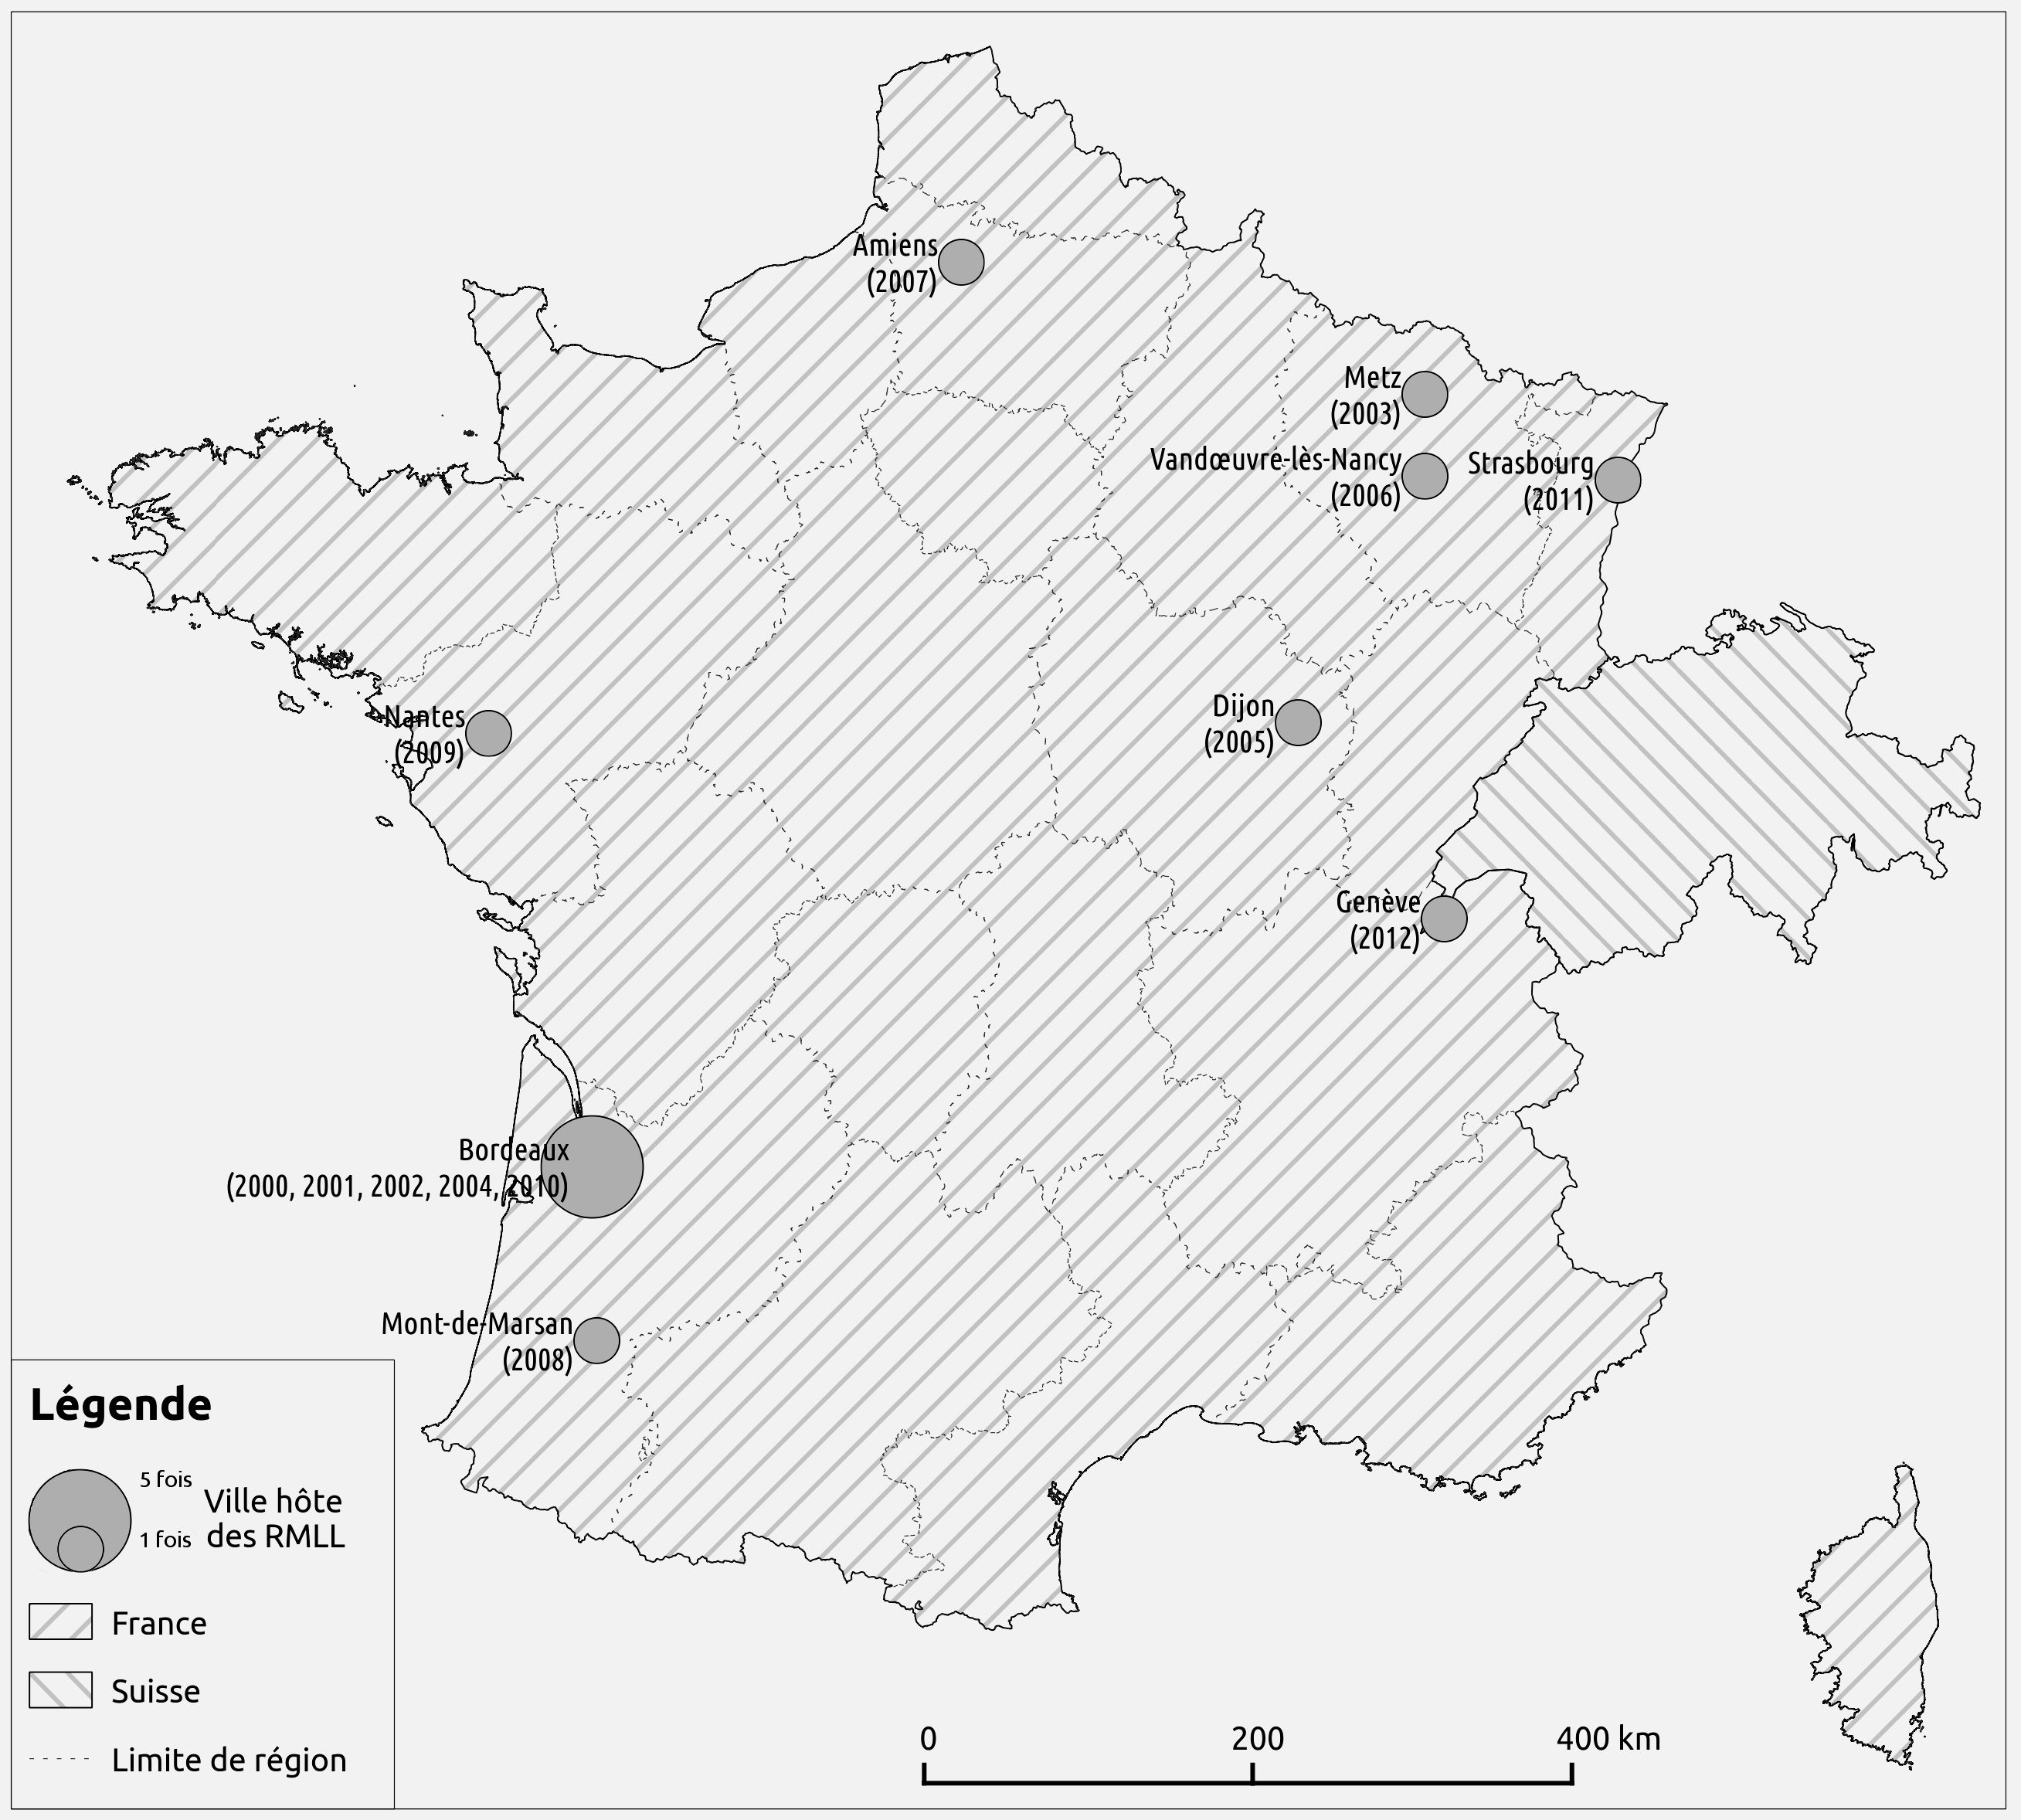
\includegraphics[scale=0.3]{images/images_PAGiraud/carte_rmll_revue.png}
\caption{Les RMLL: un seul lieu, des sites multiples}
\end{figure}



\subsection*{1.1~~~Plusieurs sites, un seul lieu : les RMLL sont un lieu mobile}
\phantomsection
\addcontentsline{toc}{subsection}{1.1 Plusieurs sites, un seul lieu : les RMLL sont un lieu mobile}

Au total, neuf villes ont hébergé les RMLL. Notons que, techniquement,
les RMLL bordelaises ont lieu surtout (voire exclusivement les
premières années) sur le campus de Talence. On ne retrouve pas cette
imprécision pour les autres éditions. Notons qu'il y a parfois un
découplage entre la ville qui donne son nom à la manifestation et la
commune qui l'accueille effectivement. C'est le cas par exemple des
RMLL de Bordeaux, qui techniquement ont surtout lieu sur la commune de
Talence. Dans le but d'attirer des conférenciers lointains, il pouvait
être préférable d'afficher un nom mondialement connu. À l'inverse,
l'édition de~2006 porte le nom de la commune qui l'héberge. Il faut
dire que Vandœuvre-lès-Nancy en est le principal financeur, et qu'elle
soigne une image de commune en pointe sur le numérique. En effet, elle
est alors l'une des trois seules municipalités françaises à détenir les
cinq~@ du label Ville~Internet. En outre, les RMLL sont à cette date
une manifestation bien connue de la mouvance du Libre, au delà même de
l'espace francophone : l'identité de la ville hôte est moins critique,
et n'est pertinente qu'au regard des infrastructures qu'elle est
susceptible~d'offrir.

Alors même que les RMLL sont aujourd'hui un lieu mobile, l'espace
géographique dessiné par les Rencontres se différencie, à la fois de
manière explicite par les modalités de sélection mises en œuvre par le
comité des RMLL, et de manière plus implicite à travers ce qui peut
apparaître comme des critères tacites de sélection.

\subsubsection*{1.1.1~~~Comment un lieu peut-il être mobile ?}
\phantomsection
\addcontentsline{toc}{subsubsection}{1.1.1 Comment un lieu peut-il être mobile ?}


Puisqu'il n'y a de lieu qu'en fonction d'intentions et de
représentations, on ne peut pas fixer de taille maximale au lieu,
au-delà de laquelle il faudrait nécessairement parler de surface. Au
contraire, le Monde lui-même peut apparaître comme un lieu\footnote{\cite{retailletransformation2011}.}, par exemple quand il est envisagé sous l'angle du réchauffement
climatique. L'inverse est également vrai : même au sein d'un tout petit
espace la distance peut être pertinente. Qui n'a jamais été trop
paresseux pour aller chercher un dictionnaire sur une étagère située à
1,50~m de son bureau ?

Deuxièmement, elle permet d'envisager des lieux sans localisation fixe.
Puisque le lieu est défini par le contact entre deux ou plusieurs
réalités, la localisation topographique de ce dernier ne change rien à
l'identité du lieu qui se manifeste –~qui, précisément,
a lieu. C'est ainsi qu'il faut comprendre l'expression
«~aller aux RMLL~» voire aux
«~ReuMeuLeuLeu~», très employée par les
participants : l'identité du lieu perdure malgré les changements de
ville~hôte et d'équipe~organisatrice.

La ville d'accueil n'est pas pour autant dépourvue de statut
géographique. La théorie de l'espace mobile \footnote{\cite{retailleespace2005}.}, qui la disqualifie comme lieu relativement aux RMLL, apporte
également la notion de site, désignant ainsi simplement ce qui
«~accueille~» ces
«~circonstances plus ou moins durables~» que sont
les lieux
\footnote{\cite[p.~20]{retailleles2012}.}.

La distinction d'avec les sites permet donc d'assurer la permanence du
lieu malgré une localisation mouvante. Elle ne permet pas, cependant,
de comprendre comment les RMLL maintiennent leur identité malgré une
équipe organisatrice propre à chaque ville~hôte. C'est plutôt du côté
des modalités d'organisation de l'événement qu'il faut aller chercher
des~réponses.

\subsubsection*{1.1.2~~~La sélection des sites par le comité : quelles modalités de différenciation de l'espace ?}
\phantomsection
\addcontentsline{toc}{subsubsection}{1.1.2 La sélection des sites par le comité : quelles modalités de différenciation de l'espace ?}

Depuis que les RMLL sont mobiles par projet
 –~c'est-à-dire
depuis~2004~– un
comité sélectionne les villes~hôte pour l'année à venir et parfois la
suivante. Il est composé de deux responsables volontaires de
l'organisation (président, vice-président, trésorier, etc.) de chacune
des quatre RMLL les plus récentes. Depuis juillet~2011, il faut y
adjoindre un représentant de la dernière édition des RMLL
décentralisées (RMLLd). Il compte donc au minimum huit puis neuf
membres. Enfin, toute personne acceptée par ces derniers à la majorité
des deux tiers peut l'intégrer. Ainsi, entre~2006 et~2010,
l'Association Francophone des Utilisateurs de Linux (AFUL) y dispose
d'un représentant. Ce comité, au temps de roulement beaucoup plus long
que celui, annuel, des équipes d'organisation à proprement parler,
assure le maintien de l'identité des RMLL à travers les années. En
outre, il permet le transfert des compétences et l'accumulation
de~l'expérience.

La procédure de sélection est formalisée, dès avant~2007, dans un
document qui reprend explicitement l'analyse multi-critères appliquée
dans les grandes entreprises. Les critères, qu'ils soient destructifs
(dont le non-respect est éliminatoire) ou sélectifs (dont le respect
est valorisé), montrent que la sélection porte simultanément sur
l'équipe d'organisation et sur le site d'accueil. Concernant le site,
il est surtout question de la capacité d'hébergement et de
restauration, mais aussi du nombre et de l'équipement des salles dans
les structures d'accueil. La «~situation
géographique~» est rapidement évoquée : c'est alors en fait de
l'accessibilité du site en train et en avion, ainsi que de sa proximité
au «~centre-ville~» dont il est question. Quant à
l'organisation, elle doit être portée par «~une ou
plusieurs associations impliquées dans la communauté du Libre~» d'au
moins vingt personnes, et compter au moins un membre de l'équipe d'une
édition~précédente.

Cette procédure est rendue nécessaire par la concurrence de plusieurs
candidatures chaque année. On peut citer, à titre d'exemple, quelques
candidatures malheureuses : Nice et Clermont-Ferrand~(2007),
Pau~(2008), Bordeaux~(2009), Toulouse~(2010), Tarare~(2012, face à
Genève après le retrait de Liège, déjà sélectionnée, durant
l'été~2011). Cependant, plus que la ville, c'est l'association qui est
sélectionnée, à travers sa capacité à monter un dossier de candidature
convainquant. En outre, les RMLL ne transforment pas le site sur lequel
elles ont lieu, mais ont pour objectif de former les militants locaux à
l'organisation d'événements et aux relations avec les collectivités
territoriales –~relations qui
doivent tout de même exister un minimum auparavant dans la mesure où
elles constituent un critère sélectif du dossier. La mobilité relève
donc d'une stratégie de pénétration des territoires par le Libre où les
bénévoles ne sont pas interchangeables, mais représentent au contraire
des agents dont il s'agit d'activer les potentialités grâce aux
compétences qui leur sont transmises par le comité et des bénévoles
d'années précédentes. Ainsi, pour François Pellegrini, membre du comité
de~2005 à~2008 :

\begin{quote}
La mobilité des RMLL est un moyen de former nos activistes à
l'organisation de manifestations, et au cours de l'organisation de
l'événement, de prise de contacts avec le monde politique local et les
médias locaux, et les acteurs associatifs locaux : les RMLL ont un rôle
pédagogique crucial dans leur nature même sur la préparation de
l'événement. Donc il est essentiel de «~faire tourner le barnum~», pour
reprendre une expression qui avait été donnée par Thierry Laronde.[...]
Aujourd'hui on a tous l'idée que faire tourner les RMLL c'est à chaque
fois éduquer les politiques locaux et mettre au service des DSI de
l'information gratuite [\ldots]. Les RMLL laissent toujours des traces.
Elles sont un outil essentiel de pénétration des territoires, donc il
est essentiel de le faire tourner.
\end{quote}

L'espace géographique est donc différencié par le comité en fonction de
la capacité d'une association locale à transformer un site en lieu des
RMLL. Dans ce cadre, la mobilité n'est pas un but en soi : elle est un
moyen de s'ancrer dans les territoires. L'espace des représentations
(la grammaire des représentations de l'espace) sous-tendu par les RMLL
met ainsi en jeu des interactions entre mobilité et ancrage, mais aussi
entre lieux et~territoires.

Ainsi, la continuité de l'identité des RMLL est assurée par le comité.
Elle leur confère une épaisseur temporelle qui laisse place à la
différence, à l'évolution : elle leur donne une histoire. Or, le lieu
n'est qu'une circonstance~passagère.

\subsubsection*{1.1.3~~~Du lieu à la localité : innovations événementielles et acculturation}
\phantomsection
\addcontentsline{toc}{subsubsection}{1.1.3 Du lieu à la localité : innovations événementielles et acculturation}

La théorie de l'espace mobile avance que les sites qui accumulent la
mémoire des lieux qu'ils ont accueillis sont des
localités\footnote{\cite[p.~20]{retailleles2012}.}. Une localité est donc le fruit d'une succession, sur un
site, de lieux sédimentés en histoire. Les RMLL sont un lieu mobile
avec une histoire. En trouvant leur site unique et les différents lieux
qu'il accueille, elles apparaîtront comme une~localité.

Pour cela, chaque RMLL doit être envisagée comme un lieu spécifique. La
dimension très discrète (par opposition à continue) de la
manifestation, qui n'a lieu que quelques jours par an, autorise cela.
De même, des innovations événementielles transforment pour certaines la
portée et le sens des Rencontres. Elles montrent que les RMLL ont
beaucoup évolué depuis leur première édition en~2000, qu'elles sont le
fruit d'une construction de treize années et encore en cours. Elles
sont aussi la preuve qu'une marge de manœuvre certaine est laissée aux
organisateurs par le comité, que les associations locales possèdent une
part de la maîtrise d'ouvrage. Parmi les innovations introduites, on
peut compter : le village associatif~(2003)\footnote{Cela désigne le
lieu constitué des stands des nombreuses associations du Libre qui se
rendent aux RMLL : APRIL, Framasoft, Wikimedia France, etc. Leur liste
est variable selon les années.}, la parole aux enfants~(2007,
abandonnée après~2009)\footnote{Il s'agit d'animations à destination
des enfants réalisées soit en partenariat avec des structures de
l'éducation populaire (2007 et~2009) soit avec des classes d'école
primaire~(2008). Les enfants sont invités à produire des contenus très
variés à l'aide de logiciels libres auxquels ils sont initiés pour
l'occasion.}, les journées grand public\footnote{Des journées sans
conférence le week-end juste après (2009 et~2010) ou juste avant (2011
et~2012) le reste des RMLL. Le but est uniquement de présenter le Libre
au grand public, à l'aide de stands, d'animations et d'ateliers.} –~à différencier des
conférences grand
public~– et le
festival des arts numériques libres~(2009)\footnote{Le terme désigne
les concerts voire les projections d'œuvres libres qui ont lieu en
marge des RMLL, notamment durant la nuit.}, la vente de bières
libres~(2011), ou encore les
\textit{lightning-talks~}(2012)\footnote{Littéralement conférences
éclairs, elles ne durent pas plus de 5~minutes chacune.}.
L'organisation des RMLLd en~2011 est également à mettre au crédit de
l'équipe strasbourgeoise, ainsi que des CÉMÉA (Centres d'Entraînement
aux Méthodes d'Éducation Active) de La~Réunion. Ces innovations
constituent une acculturation de la manifestation de l'année~\textit{n}
au contact de l'association locale qui organise celle de l'année
\textit{n}~+~1. Plus important peut-être encore, la fréquentation de
l'événement est multipliée par dix au cours de la décennie : en~2000,
les RMLL rassemblent 500~personnes, contre~5500 en~2009. Cette
croissance quantitative s'accompagne d'une transformation qualitative
de l'organisation, des conférences et du public présent. Ainsi, le lieu
mute tout en conservant son~identité.

Or, seule la mémoire permet à l'identité de perdurer malgré le temps et
l'altérité à soi-même qu'il induit. Le comité assure la mémoire des
RMLL : là où le comité se réunit (là où il a lieu) se trouve également
ce site. Chaque année il se réunit physiquement aux RMLL, mais il se
réunit aussi entre-temps grâce à divers outils aussi utilisés par les
organisateurs et les participants : \textit{mailing-lists} (listes de
diffusion), \textit{chan~IRC} (salon de discussion instantanée – Relay
Chat channels), wikis ou encore sites web. Autrement dit, si les RMLL
ont une histoire, c'est qu'il faut avec
Beaude\footnote{\cite{beaudeinternet2012}.} 
considérer Internet comme un espace géographique de plein droit, où se
trouvent des sites tout à fait capables d'accueillir des lieux et de
devenir des~localités.

\subsection*{1.2~~~D'un ancrage aquitain des RMLL à une image libriste de l'Aquitaine ?}
\phantomsection
\addcontentsline{toc}{subsection}{1.2 D'un ancrage aquitain des RMLL à une image libriste de l'Aquitaine ?}

Pour l'heure, revenons sur les innovations et acculturations que les
RMLL ont connues, et dont la mobilité est la principale. En effet, lors
de leur fondation les RMLL sont pensées pour être aquitaines,
bordelaises même : elles sont ancrées dans un territoire. Cette origine
aquitaine, connue des libristes présents aux Rencontres, demeure assez
marquée aujourd'hui encore. Elle est d'une autre nature que la touche
spécifique apportée chaque année par les équipes successives. Elle ne
saurait pas plus être rapportée aux activités touristiques organisées
lors des RMLL (visites du bassin d'Arcachon et du Médoc en~2000, du
centre historique de Nancy et du musée de la brasserie en~2006, du
château des ducs de Bretagne en~2009, ou encore du CERN en~2012).
Aujourd'hui, l'Aquitaine est la seule région à disposer d'un stand
fédérant ses différentes initiatives autour du Libre 
–~voire du numérique
en général : les pratiques observées lors des RMLL genevoises sont à
rattacher à une politique de \textit{regional branding} (assimilation de
la région à une~marque).

\subsubsection*{1.2.1~~~Dès l'origine, une volonté de promouvoir la région comme «~territoire du Libre~»}
\phantomsection
\addcontentsline{toc}{subsubsection}{1.2.1 D'un ancrage aquitain des RMLL à une image libriste de l'Aquitaine ?}

Il est encore possible de se référer à cet acte de naissance des RMLL
qu'est le courriel de Pierre Jarillon de décembre~1999. Il y est prévu
qu'elles rassemblent «~les créateurs de logiciels
libres~». Ce n'est qu'au printemps~2000, face aux demandes du Conseil
Régional d'Aquitaine (CRA), que des thématiques grand public sont
rajoutées. Le premier objectif des Rencontres est alors de
«~faire la promotion de la région et lui donner une
image de technicité~» : elles sont bien conçues comme un outil de
promotion territoriale, de regional
branding\footnote{\cite{hospersplace2004}.}. Leur second objectif, quant à lui, est de
«~faire progresser les logiciels libres~». Par le
lieu, le contact entre deux acteurs aux espaces des représentations
différents est établi, visant à produire la codétermination d'une
identité collective (les libristes sont chez eux en Aquitaine) et d'un
territoire (l'Aquitaine favorise le logiciel libre). Il s'agit donc
bien de construire, par la répétition de l'événement, un territoire du
Libre\footnote{\cite{giraudles2010}.}, d'autant qu'initialement le CRA n'accepte de financer la
manifestation qu'à la condition qu'elle devienne pérenne. Jean-Paul
Chiron et Pierre Jarillon ont ainsi dû avancer~150~000~FF~(22~500~€)
afin d'engager les premières dépenses avant que la subvention ne soit
débloquée. Les contraintes financières posées par le CRA ont donc,
d'une certaine manière, encouragé la répétition voulue de~l'événement.

Pourtant, dès~2003, les RMLL quittent Bordeaux pour Metz. Cette première
mobilité n'est pas un projet : elle est une alternative proposée de
l'extérieur à l'annulation des Rencontres cette année-là. Les
organisateurs d'alors, dans leur récit, évoquent tous une grande
fatigue à la suite de l'édition~2002 : «~on
n'arrivait pas à démarrer~», «~ça patinait~»,
«~on avait le sentiment de tourner en rond~».
L'assemblée générale du~20~décembre 2002 décide, par conséquent,
«~l'annulation de la manifestation pour~2003 et la
création d'un comité de pilotage afin de mieux préparer l'événement
en~2004~»\footnote{Compte-rendu disponible sur :
\url{http://www.abul.org/Compte-rendu-de-l-Assemblee,227.html} }.
Le~21~janvier 2003, la décision est annoncée sur
LinuxFr.org\footnote{\url{https://linuxfr.org/news/les-rencontres-mondiales-du-logiciel-libre-2003-nauront-pas-lie}.}. Peu après, un GULL lorrain propose de les organiser, idée débattue à
l'ABUL. Pour certains, cette dernière devrait garder la maîtrise de
l'événement : la mobilité est perçue comme un risque. Pour beaucoup
d'autres en revanche, elle est une opportunité de se renouveler et de
promouvoir les logiciels libres auprès d'autres collectivités
territoriales. La fréquentation par le grand public devient un enjeu,
son importance devant démontrer aux institutions et aux politiques que
le Libre est un sujet~porteur.

\subsubsection*{1.2.2~~~L'Aquitaine et Bordeaux sont bien identifiés comme berceau des RMLL}
\phantomsection
\addcontentsline{toc}{subsubsection}{1.2.2 L'Aquitaine et Bordeaux sont bien identifiés comme berceau des RMLL}

Le rôle des collectivités territoriales, notamment du CRA et du Conseil
Général de la Gironde (CG33) est unanimement souligné par les libristes
bordelais : «~sans la Région, rien n'aurait été
possible~», car elle soutient l'événement depuis le début. En~2010,
les principales collectivités territoriales concernées (région,
département, communauté urbaine) fournissent ensemble 120~000~€ sur un
budget total avoisinant les 280~000~€. Pour François Pellegrini,
«~tous les décideurs politiques de Bordeaux et
d'Aquitaine connaissent les RMLL et savent que c'est là qu'elles sont
nées~». Selon lui, elles ont un sentiment légitime de paternité des
RMLL, qui permet de «~tisser un lien affectif entre
l'Aquitaine et le~Libre~».

Cette paternité est aussi connue des participants aux RMLL, à
l'exclusion peut-être du grand public. Une liste des villes~hôte la
rappelle sur le site web de chaque édition et les discours la
mentionnent souvent. Peut-être faut-il y voir également le fruit d'un
engagement de certains individus dans les RMLL bien au-delà de
l'organisation des éditions bordelaises. Ainsi, la délégation aquitaine
est, en~2012 encore, très~conséquente.

\subsubsection*{1.2.3~~~La mobilité des RMLL au service du \textit{regional branding} numérique de l'Aquitaine}
\phantomsection
\addcontentsline{toc}{subsubsection}{1.2.3 La mobilité des RMLL au service du \textit{regional branding} numérique de l'Aquitaine}

En~2012, trois anciens présidents des RMLL participent à l'animation du
stand aquitain, situé dans le village des associations : Pierre
Jarillon~(2000 à~2002), Jean-Paul Chiron~(2004) et Jean-Christophe
Élineau~(2008). Ce stand est le seul à fédérer les initiatives d'un
territoire. On y retrouve des informations sur les GULL régionaux, mais
aussi sur ABULédu –~distribution
GNU/Linux destinée aux écoles et aux
associations~– ou
encore sur les projets en cours d'Aquinetic, le pôle aquitain de
compétences en informatique libre fondé à la suite du succès des RMLL
montoises : Jean-Christophe Élineau en est d'ailleurs le président
jusqu'à fin~2011. La participation d'acteurs du Libre à de multiples
associations de la mouvance~(GULL, groupements professionnels, pôle de
compétences, etc.) est très fréquente en Aquitaine. Elle est due à la
faiblesse des effectifs à la fois impliqués et compétents. Au delà du
Libre, le stand présente des productions mettant en valeur les
politiques numériques de l'Aquitaine, notamment des fascicules édités
par le projet RAUDIN (Recherches Aquitaines sur les Usages pour le
Développement des dIspositifs Numériques). Ce \textit{regional branding}
auprès de la mouvance du Libre s'appuie en outre sur une image de
marque déjà bien assise : celle d'une région viticole. Ainsi, des
dégustations de vin sont proposées sur le stand, à l'heure
de~l'apéritif.

\subsection*{1.3~~~Quelques ancrages plus ou moins implicites : le champ des mobilités possibles}
\phantomsection
\addcontentsline{toc}{subsection}{1.3 Quelques ancrages plus ou moins implicites : le champ des mobilités possibles}


Ayant présenté les RMLL comme un lieu mobile, il est toutefois aisé de
relever qu'elles ont toujours eu lieu en France sauf cette année. Il y
a donc, en sus de ceux définis explicitement par le comité, d'autres
critères de choix qui, jusqu'à présent, ont disqualifié la grande
majorité des sites. Ces critères peuvent même être intériorisés par les
associations locales étrangères, qui n'envisagent pas la possibilité de
candidater. Des représentations et des stratégies limitent donc le
champ de mobilité des RMLL. Tout d'abord, les Rencontres sont un
événement surtout francophone, ce qui pour plusieurs enquêtés est
plutôt en contradiction avec leur prétention mondiale. Ensuite, la
stratégie de pénétration territoriale explique en partie l'absence de
Paris, ville mondiale de premier rang, parmi les hôtes des~RMLL.

\subsubsection*{1.3.1~~~Les RMLL, un lieu du Libre francophone voire français ?}
\phantomsection
\addcontentsline{toc}{subsubsection}{1.3.1 Les RMLL, un lieu du Libre francophone voire français ?}

Les premières années, la dimension mondiale des RMLL ne fait pas débat :
il s'agit de réunir le monde du Libre en un lieu pendant quelques
jours. Les statistiques viennent à l'appui de cette idée : dès~2000,
31~nationalités sont représentées. Pourtant, aujourd'hui, la légitimité
de l'adjectif ne semble plus si assurée. Pour certains, ce n'est que
cette année, en Suisse, que les RMLL sont véritablement devenues
mondiales. Pour d'autres encore, cela n'est pas suffisant :
«~C'est un peu prétentieux de se dire mondial quand
on se balade entre Bordeaux, Strasbourg et Genève. Parce que bon,
Genève c'est pas la France, mais ça reste tout près. Franchement, je
pense qu'on pourra vraiment dire qu'elles sont mondiales quand elles
auront lieu chaque année dans un pays différent. Hors d'Europe même.~»
La mobilité engendre donc un changement de sens de la mondialité.
Caractérisée au début par la capacité des organisateurs à mobiliser des
acteurs du Libre venant de l'ensemble de la planète, elle devient
plutôt la capacité à avoir lieu en tout point du globe. En ne
sélectionnant que des villes françaises (les seules à se porter
candidates) les RMLL acquièrent l'image d'un événement français
 –~certes déjà
contenue dans le béret qu'arbore le manchot de la première affiche.
Autrement dit, le territoire national devient l'espace de référence
pour mesurer la mobilité. Un extrait du dossier
nantais\footnote{Disponible sur le site du comité des RMLL :
\url{http://comite.rmll.info/Dossiers-exemples.html} } exprime bien
cette~idée :

\begin{quote}
Le parcours des RMLL a commencé à Bordeaux (au Sud-Ouest) pour
s'aventurer dans l'Est (Dijon, Nancy), puis au Nord (Amiens) pour enfin
revenir dans le Sud-Ouest (Mont-de-Marsan). Ce tour de France semble
alors avoir oublié l'Ouest. C'est pourquoi Linux-Nantes et ses
partenaires associatifs provenant de l'ensemble de la région se
proposent d'accueillir cet~événement.
\end{quote}

La volonté de continuité entre les éditions limite le champ de la
mobilité. Il y a beaucoup de bénévoles et de conférenciers réguliers :
cette caravane des RMLL doit pouvoir se rendre sur place, et
participer. En outre, pour que le transfert de compétences et
d'expérience ait lieu, il faut que les membres du comité puissent
s'impliquer dans l'organisation de l'événement. L'espace linguistique
francophone est donc un premier ancrage. Le coût du transport en
dessine un autre : les frais de voyage des conférenciers représentent
déjà entre un tiers et la moitié du budget total des Rencontres, sans
parler des participants venant sur leurs deniers, pour qui un coût
élevé serait~dissuasif.

En outre, les RMLL ont pour volonté d'attirer le grand public. Cela
n'encourage pas les conférences dans d'autres langues que le français,
malgré les initiatives du comité pour augmenter la proportion de
communications en anglais. Développeurs et investisseurs étrangers
peuvent donc être tentés de se diriger vers des lieux concurrents des
RMLL davantage anglophones, quoique souvent à vocation plus
spécialisée, tels que le FOSDEM (\textit{Free and open source software
developers' European meeting}) ou l'OWF (\textit{Open World Forum}). Ce
dernier, sorte d'équivalent des RMLL pour la mouvance \textit{open}, a
d'ailleurs choisi une stratégie spatiale toute différente. Ayant lieu
chaque année à Paris depuis~2008, il illustre bien cet espace du marché
qui vise l'accélération des flux (de la mobilité donc) par la fixation
de lieux qui les contrôlent et les~commutent.

\subsubsection*{1.3.2~~~La mise à distance de la métropole parisienne}
\phantomsection
\addcontentsline{toc}{subsubsection}{1.3.2 La mise à distance de la métropole parisienne}

À l'inverse, les RMLL n'ont jamais eu lieu à Paris. Certes, aucun GULL
parisien n'a déposé de candidature, ce qui montre qu'il n'existe pas de
volonté de leur part d'organiser la manifestation. Cependant, il s'agit
aussi d'une stratégie du comité. Lorsque les \textit{Ubuntu-parties}
parisiennes peuvent drainer jusqu'à 5~000~personnes, autant que les
RMLL, on pourrait penser que des Rencontres dans la capitale
rencontreraient un franc succès auprès du grand public. Cependant,
c'est oublier l'objectif de pénétration des territoires qu'ont les
RMLL. Or, dans la métropole parisienne, les RMLL passeraient
inaperçues, n'auraient aucun poids, d'autant que des événements
concurrents y ont lieu, comme l'OWF ou Solutions Linux
(10~000~visiteurs en~2010). Par ailleurs, d'autres acteurs du Libre se
chargent déjà très efficacement de cette mission. L'Île-de-France est
ainsi la première région européenne pour les emplois liés aux logiciels
libres, et le pôle de compétitivité francilien System@tic comporte un
groupe thématique Logiciels Libres. Enfin, les critères destructifs
énumérés par le comité handicaperaient une éventuelle candidature de la
capitale : y trouver une structure d'hébergement d'au moins 400~places
à moins de 20~€ la nuit relève de la~gageure.

Au contraire, la modestie de la ville~hôte est perçue comme un avantage.
Jean
Peyratout\footnote{\cite[p.~25]{jessaumeles2012}.} affirme ainsi que «~les
retombées dépendent de l'implication préalable des acteurs locaux mais
sont d'autant plus modestes que la ville est importante~». À cet
égard, l'édition montoise est emblématique. Son succès est indéniable
aux yeux des acteurs : c'est «~un tour de force~»,
une «~réussite exemplaire~».
«~J'exagère à peine en disant que c'était
l'événement de l'année à Mont-de-Marsan~». L'un ajoute :
«~on a augmenté la population de la ville de 10~\%
pendant une semaine, tout simplement~». L'exactitude de cette
information est impossible à vérifier, mais le succès s'est concrétisé,
entre autres, par la fondation du pôle de compétences Aquinetic, ainsi
que par la publication du livret \textit{Sur la route des logiciels
libres} grâce à la participation du Conseil Général des~Landes.

Le comité doit cependant composer avec les candidatures qui lui sont
proposées. Mont-de-Marsan est ainsi la seule ville moyenne (aire
urbaine dont la ville centre compte entre~20~000 et 100~000~habitants)
à avoir accueilli les RMLL, alors qu'elle semble présenter le profil
idéal de la ville~hôte.

\section*{2.~~~Un haut-lieu du Libre, point d'entrée de la mouvance mondiale sur les territoires}
\phantomsection
\addcontentsline{toc}{section}{2. Un haut-lieu du Libre, point d'entrée de la mouvance mondiale sur les territoires}


Les sites successifs des RMLL dessinent donc en creux un ancrage
territorial, faisant apparaître l'espace géographique simultanément
homogène et différencié. Ce paradoxe se résout en rappelant qu'aux
RMLL, plusieurs lieux sont en réalité présents sur un même site. Les
libristes qui restent à discuter jusque tard dans la nuit des nouvelles
fonctionnalités de leur logiciel ou des politiques numériques ne
participent pas du même lieu que les participants qui viennent se
former à l'imagerie et la visualisation médicale libres, ni même que le
grand public qui vient se renseigner sur les enjeux sociétaux des
logiciels libres. Cette deuxième partie analyse les Rencontres (donc
les divise en plusieurs lieux) en fonction de leurs objectifs et des
publics visés. D'abord, pour les militants du Libre, les RMLL sont un
haut-lieu, une célébration de leur monde vécu. Ensuite, elles sont un
outil de sensibilisation des collectivités, des institutions et des
politiques. Enfin, elles cherchent à inscrire le Libre dans des
problèmes publics contemporains pour montrer que le logiciel libre est
mis au service de la~société.

\subsection*{2.1~~~Les RMLL comme conférence hacker, ou la fête comme catharsis}
\phantomsection
\addcontentsline{toc}{subsection}{2.1 Les RMLL comme conférence hacker, ou la fête comme catharsis}

L'un des objectifs premiers des RMLL est de permettre la rencontre
«~des créateurs de logiciels libres~» du monde
entier. C'est pourquoi, dès le début, elles sont également appelées
\textit{Libre Software Meeting}, la notion de monde (\textit{World})
disparaissant à la fois pour éviter l'assimilation à une multinationale
et parce que la dimension mondiale est acquise hors de France du seul
fait qu'elles ont lieu à l'étranger. À la fin des années~1990, deux
environnements de bureau libres (KDE et GNOME) s'affrontent. Pour
Pierre Jarillon, les causes du conflit ne sont au fond que des
malentendus : une rencontre entre développeurs devrait les dissiper et
produire des relations de confiance. Cette conviction, qu'il tire de
son expérience professionnelle, peut être reformulée ainsi : la
proximité spatiale des acteurs est par elle-même, et indépendamment du
contexte extérieur, génératrice d'aménités (ici la confiance). Il
s'agit de révéler ce qui rassemble, et non ce qui sépare. Les RMLL sont
donc une fête célébrant un monde vécu et permettant, le reste de
l'année, une saine collaboration entre les projets : les RMLL sont un
lieu hybride, terme qu'il faudra~expliquer.

\subsubsection*{2.1.1~~~Les Rencontres du Monde du Logiciel Libre : la célébration d'un monde vécu}
\phantomsection
\addcontentsline{toc}{subsubsection}{2.1.1 Les Rencontres du Monde du Logiciel Libre : la célébration d'un monde vécu}

Lors des entretiens, certains affirment qu'il
«~fallait qu'on puisse manger, boire, pisser
ensemble.[…] Ça
améliore beaucoup les relations.~» Cette approche rejoint celle de
Di~Méo\footnote{\cite[p.~17]{dimeogeographie2001}.}~:

\begin{quote}
la fête agit […] comme une véritable catharsis. Le plus souvent, elle
désamorce les conflits dans une sorte de rituel. Au-delà des disputes,
des inégalités, des injustices, des luttes et des clivages sociaux,
spatiaux, religieux ou politiques, ce rituel indique que l'unité du
groupe finit toujours par l'emporter. Cette unité s'impose en tant que
valeur essentielle et existentielle, autant que nécessité profonde de
survie territoriale autant que~sociale.
\end{quote}

Le terme de rituel ne paraît pas excessif, d'autant qu'à chaque édition
a lieu un «~Repas du Libre~» qui réunit principalement les
«~militants du
code~»\footnote{\cite{proulxles2006}.}. Or, pour
Gomez\footnote{\cite{gomezrepas1985}.}:

\begin{quote}
d'une manière générale, le repas est un facteur, sauf cas
pathologique, de resserrement des liens entre les individus. […] La
nourriture est chose de partage, elle joue un rôle irremplaçable pour
forger une relation durable. On ne saurait la partager de manière
neutre fût-ce avec un~inconnu.
\end{quote}

Le repas manifeste l'unité du monde du Libre : l'échelle convoquée,
consolidée, est bien celle mondiale. Pourtant, cette consolidation ne
peut se faire que par le passage à une échelle où l'espace ne peut plus
intervenir comme boucle de rétroaction négative aux relations sociales.
Depuis~2011, cette boisson symbolique qu'est la bière libre (dont la
recette et le procédé de fabrication sont publics) joue un rôle
similaire\footnote{Cela est d'autant plus vrai que pour différencier en
anglais libre et gratuit (qui se disent tous deux \textit{free}),
Richard Stallman dit souvent «~think of 'free' as in free speech, not as in
 'free beer'~». Dans son texte sur la
définition du logiciel libre, cette phrase de clarification vient même
avant la liste des quatre libertés\footnote{\cite[p.~43]{stallmanfree2002-1}.}. Il s'agit donc pour les libristes de jouer avec –~de hacker
?~– leurs propres référents culturels.}. La fête, en abolissant toutes
les distances, fait figure de lieu total : elle est une célébration,
parfois jusqu'à la religiosité. Deux participants m'ont ainsi affirmé
venir aux RMLL «~en pèlerinage~» afin de
«~croire encore qu'il y a un espoir pour
le~Libre~».\footnote{Là encore il faut faire référence à un contexte
culturel plus large, que nous n'avons pas le temps de développer ici.
Pour plus de précisions sur le sujet: \cite[p.~64-94]{keltytwo2008}; \cite[p.~85-94]{giraudles2010}.}.

Coleman\footnote{\cite{colemanhacker2010}.} montre bien comment les DebConf sont la célébration d'un monde vécu
(«~the celebration of a
lifeworld~»). Elle insiste ainsi sur la manière dont elles sont la
mise en scène ritualisée de pratiques et de représentations courantes
dans la vie quotidienne des membres, portées à un très fort degré
d'intensité par la présence physique des membres. Or, les deux
premières DebConf ont lieu à Bordeaux (DebConf~0 et DebConf~1), dans le
cadre des RMLL~2000 et~2001. Elles sont ensuite devenues complètement
indépendantes, et sont uniquement une conférence \textit{hacker} –~ici, passionnés
des techniques de l'informatique («~\textit{aficionados dedicated to the
craft of computing}~»). Elles démontrent cependant qu'une telle
conférence est au fondement de l'un des lieux des RMLL. Les Rencontres
sont ainsi une technique spatiale de «~mobilisation
des communautés
distantes~»\footnote{\cite{jullienhow2006}.}, un espace-temps extraordinaire pour favoriser la
collaboration~ordinaire.

\subsubsection*{2.1.2~~~Entre territorial et réticulaire, les RMLL sont un lieu hybride}
\phantomsection
\addcontentsline{toc}{subsubsection}{2.1.2 Entre territorial et réticulaire, les RMLL sont un lieu hybride}

Pour comprendre les RMLL, dans leur fonctionnement comme dans leurs
enjeux, il est nécessaire d'envisager Internet comme un espace
géographique. Pour cela, le concept de lieu doit être affiné, en
distinguant lieux territoriaux et lieux réticulaires. Les lieux
territoriaux mettent en œuvre des moyens d'abolition de la distance par
contiguïté. Le contact, physique, y stimule tous les sens. Avec les
lieux réticulaires, au contraire, «~la
non-pertinence de la distance est fondée sur la
connexité~»\footnote{\cite[p.~191]{Beaude2008}.}. Ce concept permet aux géographes d'investiguer cet espace
qu'est Internet. Les libristes fréquentent ce dernier avec assiduité y
compris durant les Rencontres, au point que le maintien du réseau en
état de marche est un défi majeur pour les organisateurs. Les RMLL ont
aussi lieu sur Internet, les lieux réticulaires étant d'ailleurs les
seuls sur lesquels la manifestation existe entre deux éditions.
Pourtant, par leurs pratiques, les participants saisissent du même
geste connexe et contigu, discutant par exemple sur le \textit{chan~IRC}
alors qu'ils sont dans la même pièce. Les RMLL sont donc un lieu
hybride, mêlant le territorial au réticulaire de manière si intense que
l'artificialité de la distinction (pourtant nécessaire à
l'analyse)~ressort.

L'hybridation de l'espace est générale : elle touche l'ensemble de la
société, et pas seulement la mouvance du
Libre\footnote{\cite[p.~209]{beaudeinternet2012}.}. Pourtant, dans le cas des RMLL, elle revêt un sens
particulier. Les libristes envisagent le numérique et Internet de
manière spécifique, ce qui rend l'hybridation elle-même originale. La
manifestation de cette hybridité est au cœur de la catharsis que
permettent les RMLL : partager un monde vécu, c'est avant tout partager
ses métriques (manières dont on mesure la~distance).

\subsection*{2.2~~~Les RMLL comme outil de sensibilisation et de formation des collectivités et des institutions}
\phantomsection
\addcontentsline{toc}{subsection}{2.2 Les RMLL comme outil de sensibilisation et de formation des collectivités et des institutions}

Un autre objectif des RMLL est de promouvoir l'usage et la production de
logiciels libres. Dans le cadre de l'organisation des RMLL, les
institutions sont facilement approchées. En outre, elles partagent le
fort intérêt des activistes pour l'idée de mutualisation des moyens,
«~accélérateur~» de leur adoption des logiciels
libres\footnote{\cite{elieeconomie2009}.}. Elles sont donc perçues comme des clés d'entrée pour faire
pénétrer le Libre dans les territoires. Or, les représentants locaux de
la mouvance sont justement les organisateurs des RMLL : faire pénétrer
le Libre revient à augmenter leur influence auprès des~décideurs.

\subsubsection*{2.2.1~~~Les collectivités sont perçues comme des acteurs clés pour la pénétration des territoires}
\phantomsection
\addcontentsline{toc}{subsubsection}{2.2.1 Les collectivités sont perçues comme des acteurs clés pour la pénétration des territoires}

Les collectivités, par les politiques qu'elles mènent et par les
rapports fréquents qu'elles entretiennent avec leurs administrés, ont
un fort pouvoir de prescription, y compris en matière de logiciel. Par
exemple, il faut pouvoir ouvrir facilement les documents disponibles
sur les sites institutionnels. Souvent, les quelques conseils prodigués
pour y parvenir sont suivis. C'est pourquoi la \textit{Free Software
Foundation Europe} (FSFE) vise surtout ce genre de sites web dans le
cadre de sa campagne pour la promotion des lecteurs PDF libres. La
sensibilisation des acteurs publics est donc perçue comme un moyen
d'atteindre \textit{in~fine} le grand public et les entreprises. À ce
titre, les Chambres de commerce et d'industrie (CCI) sont des
organismes souvent prisés par les organisateurs : la CCI locale est
partenaire au moins des éditions 2006, 2007, 2009 et~2011.

Par ailleurs, pour les organisateurs comme pour de nombreux militants,
la conversion des institutions au Libre est une cause citoyenne. Elle
est donc un but en soi : par exemple, équiper les mairies en logiciels
libres est présenté comme un moyen de réduire les dépenses, de mieux
dépenser l'argent
public\footnote{\cite[p.~40]{elieeconomie2009}.}. Il faut donc clairement différencier les temps de
sensibilisation et de formation. La première est réalisée en amont des
RMLL, par les organisateurs. Elle doit être efficace car elle doit
aboutir à l'octroi de subventions : on comprend pourquoi les opérations
de transfert d'expérience et de compétence débutent de nombreux mois à
l'avance, parfois plus de douze. D'une certaine manière, la
sensibilisation se poursuit pendant les RMLL, la rencontre avec
d'autres militants pouvant apporter de nouveaux éléments. En outre, la
fréquentation par le grand public peut encourager à envisager la
question comme un enjeu électoral, même secondaire. Pourtant, les RMLL
sont plutôt le temps de la formation. C'est d'ailleurs ainsi que les
organisateurs présentent les choses : un premier retour sur
investissement est fait par les partenaires publics dès lors qu'ils
bénéficient durant l'événement de formations les intéressant
directement. Il y a donc toujours un ou deux thèmes dont l'intitulé
tourne autour des termes administrations, collectivités territoriales
et politiques publiques, soit au total plus d'une dizaine de
conférences par~an.

Cette stratégie visant, à l'échelon régional voire départemental ou
communal, une diffusion \textit{top-down} des logiciels libres est
souvent couronnée de succès, surtout dans le cas de Mont-de-Marsan. La
préface du livret \textit{Sur la route des logiciels libres} est ainsi
signée par Henri Emmanuelli, président du Conseil général des Landes.
De même, la participation d'hommes politiques de premier plan montre
que les RMLL ont su imposer les logiciels libres comme un thème
(mineur) de la vie politique française, et s'imposer comme le lieu
légitime depuis lequel en parler. C'est ainsi qu'en~2006, à
Vandœuvre-lès-Nancy, une table ronde sur les brevets logiciels et la
loi DADVSI a réuni François Bayrou~(UDF) et Michel Rocard~(PS), mais
aussi Richard Cazenave~(UMP) et Martine Billard~(Verts).

\subsubsection*{2.2.2~~~Un levier pour la reconnaissance et l'influence des associations locales ?}
\phantomsection
\addcontentsline{toc}{subsubsection}{2.2.2 Un levier pour la reconnaissance et l'influence des associations locales ?}

Les cas de Mont-de-Marsan et d'Aquinetic ne sont pas isolés. Un autre
exemple possible est celui du rôle qu'ont pu jouer certains membres de
l'ABUL dans la lutte contre les brevets logiciels grâce aux~RMLL.

Entre~2000 et~2002, des membres de l'ABUL acquièrent les compétences
nécessaires au montage d'événements de grande ampleur, notamment au vu
des moyens humains dont ils disposent. Sur les questions numériques,
l'influence et la crédibilité de l'association auprès des hommes
politiques locaux croît rapidement. L'exemple le plus frappant remonte
peut-être à la première édition. En~2000, les instances européennes
réfléchissent à l'évolution des brevets en Europe : le~5~juillet, soit
le premier jour des RMLL, la Commission Européenne propose la création
d'un brevet communautaire. De même, une conférence intergouvernementale
est prévue pour novembre afin de réviser la Convention sur le Brevet
Européen (CBE) de~1973 et d'introduire la brevetabilité des
logiciels\footnote{\cite{billetbrevets2000}.}. Dans ce contexte, la conférence de Jean-Paul Smets sur ce
dernier sujet est très suivie. Notamment, Gilles Savary, alors député
européen et conseiller municipal de Bordeaux, est convaincu par les
arguments des libristes : lors de son discours de clôture, il s'oppose
publiquement aux brevets logiciels et conseille d'envoyer des personnes
faire du lobbyisme au Parlement~européen :

\begin{quote}
En tant que député européen, je me mets à votre disposition pour que
vous fassiez entendre votre voix auprès des institutions européennes,
et je vous invite et vous propose à venir dans les quatre ans qu'il me
reste au parlement européen rencontrer des députés pour les
sensibiliser à ces questions de la protection de la création et
notamment de la création des~logiciels.

Le Parlement européen est un jeune parlement qui accueille volontiers
les lobbies et vous ne devez pas laisser la place au seuls lobbies des
firmes et des~industriels.\footnote{Transcription du discours de
Gilles Savary : \url{https://www.april.org/articles/communiques/pr-lsm.html}.}
\end{quote}

François Pellegrini y est envoyé. Jusqu'à la demi-victoire des opposants
aux brevets logiciels (aucun texte n'est finalement voté), il est l'un
des conseillers de Michel Rocard sur cette~question.

Ce succès spectaculaire des RMLL pour accroître l'influence des
libristes auprès des hommes politiques locaux (qui ici ont ensuite
servi d'intermédiaires vers d'autres hommes politiques) n'est pas une
exception. À différents niveaux, sur des sujets différents, plusieurs
RMLL ont permis d'asseoir la notoriété des associations organisatrices,
de densifier leurs réseaux de relations, de faire germer des projets.
Souvent, elles bénéficient aussi, avant ou pendant la manifestation,
d'une couverture accrue dans la presse quotidienne régionale
(\textit{Sud-Ouest} pour les éditions bordelaises et montoise,
\textit{20~minutes Strasbourg} en~2011, \textit{L'Express} pour
Genève). La venue des RMLL permet donc aux associations locales
d'acquérir temporairement une visibilité pour faire valoir, sur l'aire
(régionale) de diffusion du journal, une cause pour elles~universelle.

Cependant, l'organisation d'une telle manifestation est harassante, et
les bénévoles les plus investis peuvent en sortir exsangues. Certains
GULL organisateurs ont eu du mal à s'en remettre. C'est pourquoi, par
la suite, les partenariats entre associations multiples sont favorisés
–~cela permet en outre de resserrer les liens entre lesdites
associations. En~2009 par exemple, Linux-Nantes s'associe avec Alliance
Libre : le GULL bénéficie des contacts du groupement professionnel.
Dans ce cas, la diversité de la mouvance apparaît comme une ressource
importante dans la production du lieu des~RMLL.

\subsection*{2.3~~~Une manifestation inscrite dans le monde : la prédication auprès du grand public}
\phantomsection
\addcontentsline{toc}{subsection}{2.3 Une manifestation inscrite dans le monde : la prédication auprès du grand public}

Enfin, le grand public est visé pour lui-même. Les RMLL sont un
haut-lieu du Libre francophone, perçu comme tel par les participants.
Cependant, il est aussi une interface avec un grand public à
sensibiliser voire convertir. Pour prendre une image, les RMLL sont à
la fois un lieu de pèlerinage et une terre de mission. Le premier
contact est assuré par la dimension festive de l'événement, d'autant
plus lorsqu'elle est inscrite dans l'espace public. Il peut être
prolongé par des conférences qui visent à intégrer la mouvance du Libre
aux grands problèmes publics~contemporains.

\subsubsection*{2.3.1~~~La fête comme stratégie de conquête territoriale}
\phantomsection
\addcontentsline{toc}{subsubsection}{2.3.1 La fête comme stratégie de conquête territoriale}

La fête, déjà évoquée plus haut comme célébration d'un monde vécu entre
les militants, est aussi un vecteur de conquête territoriale auprès du
grand public. En~2010 par exemple, des présentations sont organisées
dans des cinémas. Le festival des arts numériques libres relève aussi
de cette stratégie : il s'agit d'utiliser la fête pour produire du
contact (donc du lieu) avec le grand public et en profiter pour essayer
de le sensibiliser voire de le faire venir à des conférences
accessibles sans bagage technique. Dès lors, la localisation fine des
sites au sein de la ville~hôte est très importante, tout comme
l'occupation de l'espace public en amont de l'événement à l'aide
d'affiches ou de manifestations en rapport avec le Libre. C'est ainsi
que l'on peut interpréter l'affluence bien plus faible du grand public
à Genève qu'à Bordeaux. En~2010, de nombreuses affiches sont disposées
dans la CUB, surtout à Bordeaux même et Talence, plusieurs semaines à
l'avance. Le week-end grand public est organisé sur les quais, à
proximité du skate-parc, c'est-à-dire un lieu fréquent de pause sur
l'un des parcours de promenade préférés des Bordelais. À Genève, s'il
est vrai que des publicités dans les tramways annoncent la tenue des
RMLL, l'occupation de l'espace public est beaucoup plus discrète, pour
ne pas dire invisible. La salle communale de Plainpalais, où se déroule
le week-end grand public, semble à l'écart des lieux de
loisirs~genevois.

Cela change le sens de l'événement, en faisant varier l'importance de
l'une de ses dimensions. À Bordeaux, les RMLL sont inscrites dans la
vie des festivals, jouent leur rôle d'interface
«~entre les geeks et toutes les variétés de
non-geeks~», pour reprendre une formule de François Pellegrini. À
Genève, l'édition~2012 est davantage hors-sol, sans interaction
véritable avec le grand public. Cela n'enlève rien au succès des deux
dimensions des RMLL évoquées plus hauts. Plusieurs participants
évoquent même le très bon niveau des conférences et soulignent la
qualité de~l'organisation. 

\subsubsection*{2.3.2~~~L'inscription du Libre dans de grandes questions de société}
\phantomsection
\addcontentsline{toc}{subsubsection}{2.3.2 L'inscription du Libre dans de grandes questions de société}

Les thèmes abordés constituent l'autre élément de la stratégie des RMLL
à destination du grand public. Les organisateurs veulent montrer que le
Libre est important au-delà du logiciel : qu'il est porteur d'un modèle
de société libre, ou au moins qu'il vise à mettre les logiciels au
service de la société. Des thèmes choisis chaque année, transversaux ou
non, répondent à cette exigence. Par exemple, l'édition~2000 traite la
question du développement (économique). L'espace visé est surtout
l'Afrique. L'un des résultats de ces premières RMLL est d'ailleurs la
création de l'Association Africaine des Utilisateurs de Logiciels
Libres (AAUL). Les questions d'éducation (populaire ou non), la santé,
l'économie, la culture ou encore le développement durable et
l'accessibilité (thèmes transversaux en~2010) dénotent ainsi une
volonté d'inscrire le Libre dans les problèmes publics~contemporains.

Cela montre que, pour les militants, les logiciels –~\textit{a~fortiori}
ceux qui sont libres~– ne sont pas des outils neutres, qu'ils sont
porteurs d'un sens politique et d'une manière d'être au monde. Il
s'agit, autrement dit, de les introduire eux-mêmes comme problème
public –~au sens où le \textit{probouleuma} désigne dans la \textit{polis}
athénienne une proposition présentée au Conseil, et qui par conséquent
fait débat\footnote{NdE : \textit{probouleuma}, équivalent d'une proposition de loi présentée devant
la \textit{Boulè}, conseil de citoyens --~initialement tirés au sort~-- en charge du
gouvernement. Ce sont les premières formes de démocratie politique.}.
L'hybridation de l'espace géographique contemporain rend cette
introduction d'autant plus nécessaire.

\subsubsection*{2.3.3~~~Les limites des RMLL : horizon, ou confins ?}
\phantomsection
\addcontentsline{toc}{subsubsection}{2.3.3 Les limites des RMLL : horizon, ou confins ?}

Plusieurs lieux se superposent au cours des RMLL : le lieu de la
conférence technique, celui de la formation et de la sensibilisation
des collectivités, enfin celui de la rencontre grand public. Ces trois
lieux, qui sont en interaction, ne relèvent pourtant pas du même espace
de représentation, dans la mesure où c'est justement cet espace de
représentation commun que les RMLL visent à produire. Vers l'intérieur,
la dimension spatiale de ces lieux est identique, dans la mesure où la
distance n'y est pas pertinente. En revanche, ils se différencient par
la relation qu'ils entretiennent avec l'espace qui les englobe, et donc
par la forme de leur
limite\footnote{\cite{retailletransformation2011}.}.

D'abord, en tant que conférence \textit{hacker}, les Rencontres ont la
prétention de manifester un monde du Libre (comme le laissait entendre
un nom un temps avancé pour les RMLL : \textit{Libre World}) qui recouvre
l'intégralité du Monde. Un tel lieu peut être tout à fait mobile, à
l'image de son \textit{spin-off} que sont les DebConf. Le site qui les
héberge et la localité à laquelle il participe est indifférent à ce qui
se passe à l'intérieur du lieu. La limite du lieu se dérobe donc
toujours, aussi bien pour les participants que pour l'observateur :
c'est un \textit{horizon} (première forme de la limite). On est donc
toujours à l'intérieur du lieu qui se manifeste (le monde du Libre), ce
qui signifie aussi que même en n'étant pas sur site on participe
au~lieu.

Ensuite, en tant qu'outil de prédication et de pénétration des
territoires, les RMLL apparaissent comme des missions (dans le sens par
exemple des missions jésuites d'Amérique du Sud) temporaires. La
différence de valeur entre l'intérieur (qui justement porte les valeurs
à promouvoir) et l'extérieur est postulée. Le territoire d'accueil y
est vu comme un espace à «~libérer~» dont il s'agit de changer la
nature pour en faire un territoire du Libre –~c'est en ce sens que la
conversion de collectivités au Libre peut relever de la catastrophe (au
sens de René Thom : transformation soudaine et profonde) territoriale\footnote{\cite[p.~36]{giraudles2010}.}. La limite de ce lieu prend donc la forme des
\textit{confins} (deuxième forme).

Enfin, les RMLL adoptent en partie les \textit{frontières} (troisième
forme) des collectivités territoriales partenaires, à la fois à travers
les formations destinées à leurs personnels, la part importante
qu'elles jouent dans le financement de l'événement et car elles sont
perçues comme un acteur clé pour la «~libération~» des territoires. Les
collectivités territoriales ont bien une limite repérable, mais à la
différence de ce qui se passe pour les confins, elles sont toutes de
même nature (ce qui explique qu'on puisse les juxtaposer si elles
relèvent du même échelon, ou bien les emboîter si elles sont de
niveau~différent).

Ces trois lieux se manifestent simultanément et mobilisent pour une part
les mêmes acteurs, qui n'y voient rien à redire. C'est que si plusieurs
lieux peuvent se produire au même moment sur le même site, il est aussi
possible d'être en même temps dans tous ces~lieux.

\section*{3.~~~Les RMLL, lieu privilégié d'observation de la mouvance}
\phantomsection
\addcontentsline{toc}{section}{3. Les RMLL, lieu privilégié d'observation de la mouvance}

Pour synthétiser, les RMLL sont un haut-lieu mobile du Libre francophone
qui vise, à travers l'organisation d'une double rencontre entre
libristes et entre les libristes et le grand public, à pénétrer les
territoires régionaux. Elles confèrent ainsi une légitimité aux
associations locales face aux partenaires~institutionnels.

Nous avons montré les co-constructions des représentations, stratégies
et espaces (lieux comme territoires) à l'œuvre aux RMLL. Les différents
lieux qui y sont co-présents interagissent pour former les RMLL,
répondant chacun à un objectif déterminé. Depuis le comité qui assure
la mémoire des RMLL et le transfert de compétences jusqu'au grand
public à conquérir en passant par la célébration d'un monde vécu, tout
concourt à montrer que les libristes possèdent un espace des
représentations hybride, capable de mettre à profit les potentialités
relationnelles des espaces géographiques indépendamment de leurs
métriques. Bien que l'hybridation soit aujourd'hui en voie de
généralisation, les militants du code sont parmi les seuls à refuser de
laisser Internet hors du champ du politique. L'observation de leurs
pratiques permet de déceler des signaux faibles mais aussi, par
contraste, de pointer des dangers d'une manière de n'aborder le
numérique que par ses littoraux visibles, laissant l'essentiel du
continent à l'état de \textit{terra~incognita} à la merci d'acteurs dont
les intérêts ne sont pas forcément ceux des~citoyens.

\begin{figure}
\centering
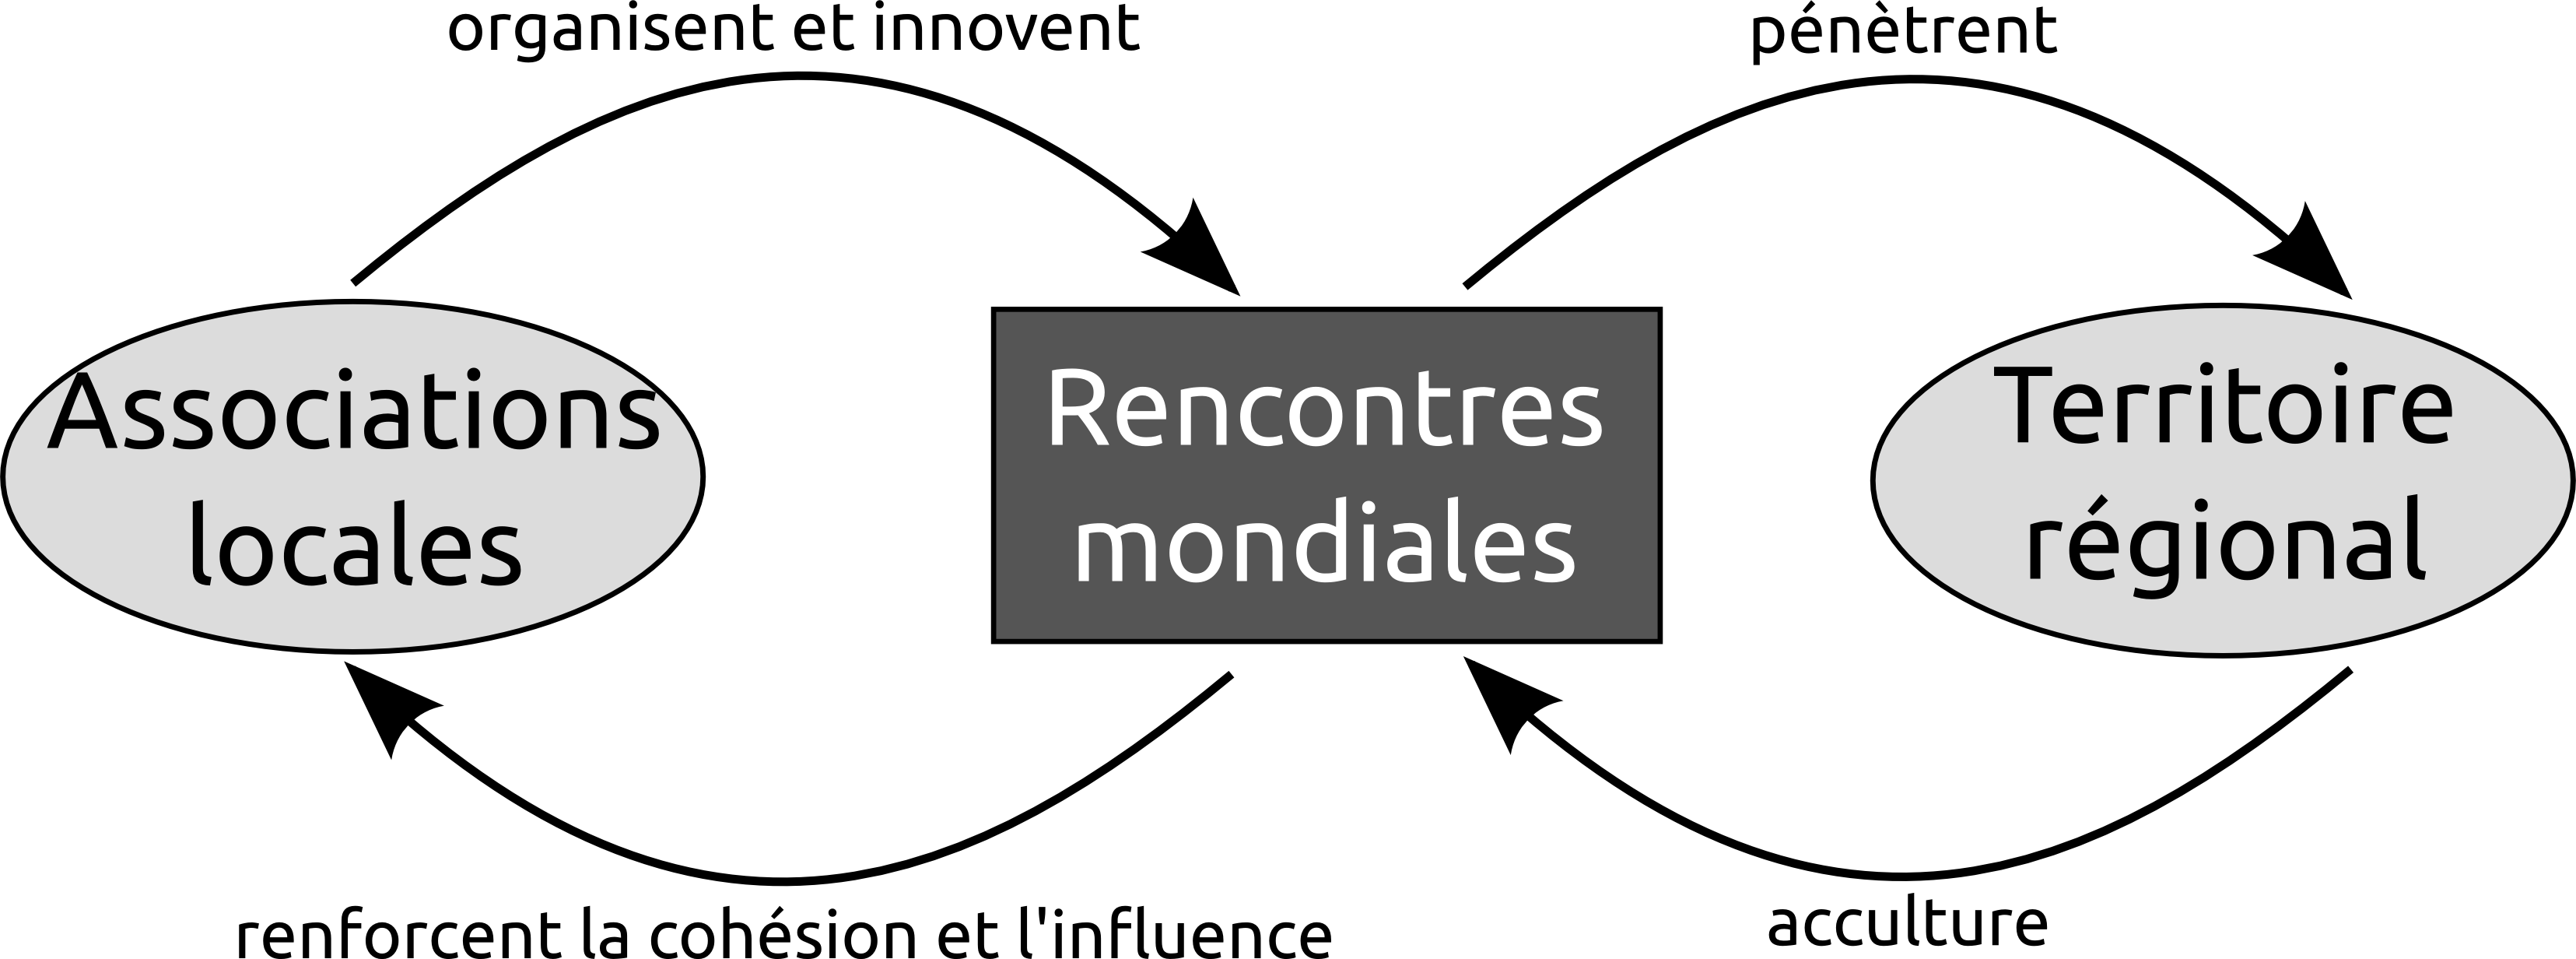
\includegraphics[scale=0.3]{images/images_PAGiraud/rmll_interface_revue.png} 
\caption{Jeux d'échelons et d'interface au lieu des RMLL}
\end{figure}

Les évolutions des RMLL témoignent aussi des transformations du Libre au
cours de la décennie passée. Le profil des associations organisatrices
change, reflétant l'acculturation du Libre dans la société mais aussi
la perte relative d'importance des GULL dans le mouvement associatif du
Libre (puisqu'ils n'en sont plus les seuls acteurs). Ainsi,
jusqu'en 2007, les organisateurs ne sont que des GULL. De 2008 à 2010,
des GULL sont porteurs, épaulés par d'autres associations de la
mouvance. En~2011 et~2012, les associations porteuses ne sont plus des
GULL : ce sont sont eux qui désormais~épaulent.

Finalement, d'abord centrées exclusivement sur les logiciels, les
Rencontres se sont élargies jusqu'à inclure des productions
culturelles, du matériel et même des données. Cet élargissement du
champ du Libre, qui avec des pratiques amène des cultures et des mondes
vécus nouveaux, questionne sans cesse ce qui fait l'unité de la
mouvance, alors même que son orientation générale semble conservée.
C'est donc à juste titre que
Kelty\footnote{\cite{keltytwo2008}.} a pu qualifier les mouvements dérivés de celui du logiciel libre de «~modulations~». Les opportunités en sont l'enrichissement et
la fertilisation croisée, les risques en sont la disparition d'un sens
commun même minimal du Libre ainsi qu'une perte de lisibilité de la
mouvance, déjà complexe pour le grand public. Quelle image du Libre un
visiteur peut-il avoir quand il vient d'assister, aux RMLL, à une
conférence présentée à l'aide d'un programme propriétaire ? En se
modulant, le Libre a pu accroître sa diffusion auprès de divers milieux
professionnels et culturels, ainsi que d'une partie du grand public.
Pourtant, son succès risque de se faire au détriment des valeurs et des
pratiques des développeurs qui ont initié le mouvement. Ce n'est pas un
échec des RMLL : elles ne font que rendre visible, en la condensant, la
mouvance du Libre dans toute sa diversité. L'absence de certitude
concernant les pratiques et les valeurs constitue justement l'un des
indices de l'espace mobile et justifie le terme même de mouvance : on
ne peut jamais dire si l'on est dehors, ou bien si l'on est dedans.






                    
\printbibliography[heading=subbibliography]
\end{refsection} 



% -------------------------------------------------------------------------
%
%%%%%%%%%%%%%%%%%%%%%%%%%%%%%%%%%%%%%%%%%%%%%%%%%%%%%%%%%%%%%%%%%%%%%%%%%%%%
%
\part{Trajectoires du Libre}
\phantomsection
%\addcontentsline{toc}{part}{Trajectoires du Libre}
%
%%%%%%%%%%%%%%%%%%%%%%%%%%%%%%%%%%%%%%%%%%%%%%%%%%%%%%%%%%%%%%%%%%%%%%%%%%%%
%
%--------------------------------------------------------------------
\chapter*{Influence du Libre dans l'histoire du jeu vidéo}   
\phantomsection                
\addcontentsline{toc}{chapter}{Influence du Libre dans l'histoire du jeu vidéo \\ \textit{Damien Djaouti}}
%--------------------------------------------------------------------

\fancyhead[LO]{\small Influence du Libre dans l'histoire du jeu vidéo}
\fancyhead[RE]{\small Damien \textsc{Djaouti}}
%%\setcounter{section}{0}
\begin{refsection}

\begin{flushright}
Damien \textsc{Djaouti}
\end{flushright}
\vspace{10 mm}

À première vue, la définition du logiciel libre semble en tout point
contraire à celle des jeux vidéo disponibles dans le commerce. En
effet, pour reprendre les termes de la
FSF (Free Software Fundation) :
«~L'expression «~logiciel libre~» veut dire que le logiciel respecte la
liberté de l'utilisateur et de la communauté. En gros,
\textit{les utilisateurs ont la liberté
d'exécuter, de copier, de distribuer, d'étudier, de modifier et
d'améliorer le logiciel}~»\footnote{Relevé le 16-07-12 à partir de
\url{http://www.gnu.org/philosophy/free-sw.fr.html}.}. Or, dans le cas
des jeux vidéo, il s'agit de logiciels dont le code source n'est pas
accessible, empêchant ainsi toute initiative d'étude, de modification
ou d'amélioration. De même, leur nature commerciale empêche aussi leur
copie et leur libre distribution. Enfin, effet de bord issu des mesures
techniques de protection contre la copie\footnote{Les systèmes de
type Digital Rights Management (DRM) sont des dispositifs techniques
limitant par exemple le nombre d'installations possibles d'un jeu vidéo
à partir de chaque exemplaire acheté, ou encore qui empêchent
l'exécution d'un programme de jeu si l'utilisateur n'est pas connecté à
Internet afin de valider l'unicité de son exemplaire. Pour plus de
détails, voir la page Wikipédia \url{http://fr.wikipedia.org/wiki/Gestion_des_droits_numériques}.},
la liberté d'exécution de la plupart des jeux vidéo commerciaux actuels
est également de plus en plus restreinte. Sur ordinateur, les jeux
vidéo achetés dans le commerce ne peuvent être installés que sur un
nombre limité de machines différentes ; tandis que le secteur des
consoles de jeux vidéo oblige parfois l'utilisateur à posséder une
machine spécifique s'il souhaite jouer à certains titres
populaires\footnote{Politique d'exclusivité
de certains titres très populaires (\textit{Mario}, \textit{God of
War}, \textit{Zelda}, \textit{Gran Turismo}, \textit{Halo}...) sur une
console donnée afin d'augmenter ses ventes.}.

Pourtant, cette industrie, dont le modèle économique repose sur une
logique «~propriétaire~» doit, indirectement, sa naissance au logiciel
libre, ou tout du moins à sa philosophie. À travers ce chapitre, nous
proposons de revenir aux prémices de l'histoire du jeu vidéo. Si ses
débuts commerciaux s'accompagnent ensuite de l'arrivée massive du
logiciel propriétaire, l'influence du logiciel libre ne disparaît pas
pour autant. Ainsi, nous aborderons également deux autres influences
notables du Libre dans l'histoire du jeu vidéo. Tout d'abord, la
pratique du \textit{modding}, qui consiste à
modifier des jeux existants ; puis la création de jeux vidéo en
amateur, qui culmine aujourd'hui à travers le \textit{Jeu 2.0}. L'étude de ces trois
aspects de l'histoire du jeu vidéo nous permettra d'analyser les
différents types d'influence du Libre sur le jeu vidéo.




\section*{1.~~~Le Libre comme philosophie originelle des jeux vidéo ?}
\phantomsection
\addcontentsline{toc}{section}{1. Le Libre comme philosophie originelle des jeux vidéo ?}



\subsection*{1.1~~~Les premiers jeux vidéo}
\phantomsection
\addcontentsline{toc}{subsection}{1.1 Les premiers jeux vidéo}



Les tous premiers jeux vidéo recensés à ce jour sont le résultat de
travaux de chercheurs travaillant dans des laboratoires universitaires
britanniques ou américains\footnote{\cite{djaoutiles2010}.}. 

Par exemple, le premier jeu sur
ordinateur connu à ce jour pour utiliser un affichage sur écran vidéo
est \textit{OXO}. Créé en~1952 par Alexander
Shafto Douglas, il s'agit d'un jeu de morpion tournant sur l'ordinateur
 EDSAC. La motivation première de
Douglas pour la création de ce jeu vidéo était la recherche
scientifique, \textit{OXO} venant illustrer
son mémoire universitaire sur l'Interaction Homme-Machine (IHM). En
effet, si son principe de jeu est enfantin, \textit{OXO} constitue un véritable tour de
force technique. La particularité de
l'EDSAC provient de sa capacité à
stocker des programmes en mémoire (comme la RAM de nos ordinateurs
actuels). L'appareil possède ainsi trois écrans CRT qui affichent
l'état courant de la mémoire sous forme graphique. Le génie de Douglas
a été de détourner cette fonctionnalité de contrôle de la mémoire en
moyen de synthèse graphique. Un écran CRT de contrôle, d'une résolution
de 35x16, est alors programmé pour afficher une grille de morpion ainsi
que les signes déposés par les joueurs, permettant donc de visualiser
l'état de la partie. De plus, sur le panneau de contrôle de
l'ordinateur est équipé un téléphone à cadran rotatif. Le chercheur
l'utilise comme «~manette de jeu~». Ce cadran comporte des numéros
allant de~0 à~9, tandis qu'une grille de morpion est composée de
9~cases. Il numérote donc les cases de la grille de~1 à~9 en commençant
par celle située en haut à gauche. Pour jouer, l'utilisateur doit alors
composer un numéro sur le téléphone afin d'indiquer dans quelle case il
veut déposer son signe. Comme la plupart des projets des pionniers de
l'informatique, le code source d'\textit{OXO} est accessible sans restriction. Pour autant, malgré l'ouverture de
son code source, le partage d'\textit{OXO} se heurte à l'époque à une
réalité matérielle qui limitera considérablement la diffusion de ce jeu
vidéo : en~1952, il n'existe qu'un seul ordinateur de type EDSAC à travers le monde, celui de
l'université de Cambridge où Douglas effectue
ses études…


Les laboratoires universitaires ont permis la naissance de plusieurs
autres jeux sur ordinateur, tels que
\textit{Tennis For Two} (1958), un jeu de
tennis pour deux joueurs, ou \textit{HUTSPIEL} (1955), un jeu de stratégie au tour par tour destiné à la formation
des généraux de l'armée américaine. Mais aussi innovants et
intéressants qu'ils soient, ces jeux vidéo n'auront finalement qu'une
influence très modeste dans l'histoire du jeu vidéo, à cause de leur
diffusion confidentielle. Il faut alors attendre l'année~1962, pour
voir apparaître un jeu vidéo «~de laboratoire~» qui a eu une influence
notable : \textit{Spacewar!}\footnote{\cite{djaoutiles2010-1}.}. Au début des années~1960, le
Massachusetts Institute of
Technology (MIT), célèbre université américaine spécialisée dans la
recherche technologique, héberge parmi ses nombreux étudiants une
poignée de génies animés par un esprit de création et d'innovation
technologique : les \textit{hackers}. Si
aujourd'hui le terme hacker est souvent associé aux «~pirates
informatiques~», dans les années~1960 ce terme ne possède encore qu'une
acceptation noble : il désigne des bidouilleurs experts en électronique
et en informatique\footnote{\cite{levyhackers1994}.}. Au MIT, le point de rassemblement des
hackers est un club d'étudiants dédié au modélisme ferroviaire, le Tech
Model Railroad Club (TMRC). Dans une grande pièce, ses membres passent
des heures à créer les tracés ferroviaires les plus complexes et
originaux qui soient. Si cette tâche ne nécessite \textit{a~priori} que
des compétences en électronique, l'informatique deviendra rapidement un
autre terrain d'expérimentation du club. Bidouillant tout d'abord un
vieil \textit{IBM~709} laissé à l'abandon
dans les couloirs du MIT, les membres du TMRC s'épanouissent réellement
à partir de~1959, année d'acquisition d'un ordinateur
\textit{TX-0} par le MIT. Équipé d'un écran
CRT avec crayon optique, l'appareil est rattaché à l'Artificial
Intelligence Group, un groupe de chercheurs en intelligence
artificielle dirigé par les professeurs John McCarthy et Marvin Minsky.
Leurs étudiants s'accaparent immédiatement la quasi-totalité des
créneaux vacants sur le planning d'utilisation de la machine, soit la
plage horaire allant de 23~h du soir à 7~h du matin. Une bonne partie
de ces étudiants étant des membres ou des sympathisants du Tech Model
Raildroad Club, le \textit{TX-0} devient
rapidement leur terrain d'expérimentation favori. Poussés par une
recherche de la performance technique, ils y créent divers programmes,
dont des jeux tels que \textit{Mouse in a Maze} (Ross \& Ward, 1961), \textit{Tic-Tac-Toe} (Daly, 1961) ou encore \textit{Qubic} (Daly, 1961). Fidèles à
une philosophie de partage et de diffusion de la connaissance, tous les
programmes des hackers sont «~ouverts~». Leur code source est librement
accessible, ce qui permet à chaque hacker d'améliorer les programmes et
jeux écrits par d'autres, avant de partager à son tour la version
améliorée du logiciel. Concrètement, cela signifie que les cartes
perforées sur lesquelles sont enregistrés les codes sources de ces
différents programmes sont stockées dans un placard qui n'est
volontairement pas fermé à clé, afin que tout le monde puisse y avoir
accès\footnote{\cite{graetzorigin1981}.}. S'il est trop tôt pour parler d'Open-source,
voire de logiciel libre\footnote{La formalisation des notions de
Libre et d'Open-source n'ayant eu lieu qu'à partir des années~1980.},
nous reconnaissons clairement ici une volonté d'ouverture et de partage
de codes sources qui se retrouve aujourd'hui dans la philosophie du
Libre. Pourtant, malgré cette ouverture, l'influence de ces quelques
jeux créés par les hackers du TMRC resta pour lors limitée aux seuls
membres du club.

\subsection*{1.2~~~Spacewar!}
\phantomsection
\addcontentsline{toc}{subsection}{1.2 Spacewar!}


À l'automne~1961, le \textit{TX-0} se voit
doté d'un compagnon de jeu, le \textit{PDP-1} du constructeur
DEC. Encore plus puissant que le \textit{TX-0},
ce nouvel ordinateur est également mieux équipé. Plus petit, il est
également plus facile d'accès, sa mise en route pouvant être effectuée
par une personne seule. Le \textit{PDP-1} propose en standard un écran
CRT, une imprimante, un crayon optique et surtout une mémoire
impressionnante de 4K. Seul problème, comme le \textit{TX-0} à son arrivée, il n'existe
aucun programme pour cette machine. Ce terrain d'expérimentation vierge
ne laissa pas insensible les hackers du TMRC, et les conduisit même à
inventer un jeu vidéo pionnier qui, cette fois, a marqué l'Histoire : \textit{Spacewar!}

Réalisé entre~1961 et~1962 pour le \textit{PDP-1}, \textit{Spacewar!} est un jeu de combat
spatial pour deux joueurs. Le concept du jeu est imaginé en~1961 par
trois étudiants du MIT qui habitent en collocation et fréquentent tous
le TMRC : Stephen~R. Russell, J. Martin Graetz et Wayne Wiitanen. Ce
dernier doit malheureusement accomplir son service militaire avant que
la réalisation du jeu ne commence. Steve Russel devient alors le
programmeur principal, assisté par Martin Graetz. Après 200~heures de
travail, les deux compères obtiennent une première version du jeu au
mois de février~1962\footnote{\cite{graetzorigin1981}.}. Deux vaisseaux, un stock d'essence
limité et une réserve de missiles, il s'agit d'une version épurée mais
efficace du concept originel. Chaque joueur se déplace librement dans
l'espace et doit essayer de détruire l'autre vaisseau avec ses
missiles. En somme, il s'agit là du
premier \textit{shoot'em up}\footnote{Jeu
vidéo dans lequel on incarne un vaisseau spatial qui doit en détruire
de nombreux autres à coup de lasers.} de l'histoire\footnote{\cite{kentultimate2001}.}. 

À partir de ce moment commence un processus de design
itératif\footnote{Processus de création découpé en étapes successives
visant à créer un objet de plus en plus complet.}, où
 \textit{Spacewar!} évolue par petites touches: le jeu est testé par le groupe de hackers, on note les idées
d'amélioration, on les implémente, puis on re-teste. Le premier
problème ainsi identifié sur cette version du jeu est lié au fait que
la partie se déroule sur un fond noir, ce qui rend difficile
l'appréciation de la vitesse des vaisseaux. Russell rajoute donc un
fond étoilé aléatoire. Mais les hackers sont aussi des gens
perfectionnistes. À ce titre, Peter Samson, un autre membre du TMRC,
n'aime pas ce champ d'étoiles généré aléatoirement. Il se met alors en
tête d'ajouter au programme la représentation des étoiles véritablement
visibles dans le ciel, en respectant leurs positions et leurs
luminosités. Un rien moqueur, le groupe de hackers nomme cette
fonctionnalité «~Expensive
Planetarium~»\footnote{«~Planétarium
hors de prix~».}, pour rappeler qu'ils utilisent un ordinateur coûtant
120~000~\$ afin de dessiner une simple carte du ciel. Cette anecdote
illustre d'ailleurs à merveille la dimension «~partage et amélioration
participative~», aujourd'hui pilier de la philosophie du Libre, qui se
retrouve dès les années~1960 dans \textit{Spacewar!}.


Cette philosophie du Libre changea ainsi la nature du jeu pour le faire
évoluer vers la forme que nous connaissons aujourd'hui. En l'état, la
première version manque quelque peu de finesse : le jeu consiste tout
simplement à se déplacer le plus vite possible tout en tirant un
maximum de missiles afin d'avoir une chance de toucher l'adversaire.
Dan Edwards, également membre du
club de hackers, rajoute ensuite au
jeu la gestion de la gravité pour le rendre plus stratégique. Ce
faisant, il introduit un élément essentiel : l'étoile qui se trouve au
centre de l'écran et qui attire inexorablement les vaisseaux des
joueurs. Ce nouvel ajout chamboule complètement l'expérience de jeu,
les joueurs devant maintenant faire attention à leurs déplacements, et
penser à leur survie autant qu'à détruire l'adversaire. En d'autres
termes, le jeu devient alors un excellent compromis entre action et
stratégie, comme en témoigne son succès au sein de groupe. Martin
Graetz se charge de rajouter une dernière fonctionnalité au jeu : le
déplacement en hyper-espace. En appuyant sur un bouton dédié, le
vaisseau disparaît de la scène de jeu et réapparaît à un endroit
aléatoire. Très pratique pour éviter un missile trop proche, cette
option n'est pas sans risque car elle peut vous faire réapparaître au
beau milieu de l'étoile centrale, synonyme de mort immédiate. Ainsi, au
mois d'avril~1962,  \textit{Spacewar!} est
terminé. Mais si le jeu en lui-même est aussi révolutionnaire
qu'amusant, son maniement à partir de boutons à presser sur le \textit{PDP-1} n'est pas des plus pratique.
Qu'à cela ne tienne, Alan Kotok et Bob Saunders, membres éminents du
TMRC, utilisent des pièces de modélisme ferroviaire pour bricoler des
boîtiers de commandes adéquats !


\begin{figure}
\centering
\includegraphics[scale=0.06]{images/images_djaouti/Djaouti_SpacewarNB.jpg}
\caption{\textit{Spacewar!} tournant sur un PDP-1. (Par Joi Ito, sous licence Creative Commons -By 2.0)}
\end{figure}

Ce jeu est un succès incontesté au sein du club, les hackers passant
dorénavant de nombreuses heures à jouer à \textit{Spacewar!} quand il ne programment
pas. Ce fut également un succès lors des journées portes ouvertes du
MIT, en mai~1962, événement pour lequel un système de score fut rajouté
au jeu afin de limiter la durée de chaque partie (Graetz, 1981). Si les
acteurs principaux de ce monument de l'histoire du jeu vidéo finissent
par quitter le MIT, la nature ouverte du jeu lui assure une vie propre.
Le jeu se répand au sein des diverses universités américaines, de
nouvelles variantes (ciel qui tourne, missiles sensibles à la gravité
de l'étoile, boucliers….) étant créées à chacun de ces voyages. Mais ce
jeu connaît également une application «~utilitaire~» on ne peut plus
inattendue. DEC, le constructeur du \textit{PDP-1}, était en étroite relation
avec les étudiants du MIT, et n'hésitait pas à leur fournir des
programmes\footnote{DEC a par exemple
fourni des routines de fonctions «~sinus / cosinus~» que Russel
utilisera pour \textit{Spacewar!}.}. En échange, le constructeur
récupérait le travail de ces hackers de génie et l'exploitait comme bon
lui semblait. Ainsi, \textit{Spacewar!} fut
logiquement mis en avant par le service commercial de DEC  pour vanter les capacités de sa
machine\footnote{\cite{chaplinsmartbomb2005}.}. Mais surtout, il fut utilisé comme
programme de test pour vérifier son bon fonctionnement. Contrairement à
la RAM de nos ordinateurs actuels, la mémoire centrale du
\textit{PDP-1} n'est pas volatile, ce qui
signifie qu'un programme qui y est chargé reste présent après
l'extinction de l'appareil. Au sortir de la chaîne de fabrication du
\textit{PDP-1}, les ingénieurs chargeaient
donc \textit{Spacewar!} dans la mémoire de
l'ordinateur. Après livraison de la machine au client, l'installateur
l'allumait et, si le jeu était encore en mémoire et parfaitement
fonctionnel, cela prouvait que la machine n'avait pas subi de problème
matériel lié à son transport ou à son installation\footnote{\cite{levyhackers1994}.}.

\subsection*{1.3~~~De la libre diffusion à la logique propriétaire : la naissance d'une industrie}
\phantomsection
\addcontentsline{toc}{subsection}{1.3 De la libre diffusion à la logique propriétaire : la naissance d'une industrie}


De par sa large diffusion au sein des universités américaines,
nombreuses sont les personnes à avoir pu jouer à
\textit{Spacewar!}. Parmi ces joueurs,
certains furent inspirés et se lancèrent dans la réalisation de leur
propre jeu vidéo. Mais ces joueurs étaient animés par un esprit plus
proche de la recherche de profit qui motive les entrepreneurs que celui
de partage propre aux hackers\footnote{\cite{bartonhistory2009}.}.


Le premier jeu influencé par  \textit{Spacewar!} est à ce jour le plus ancien jeu vidéo de type «~borne d'arcade~» connu. Il s'agit tout simplement d'une version du code originel de \textit{Spacewar!} qui a été reprogrammée sur
un ordinateur \textit{PDP-11}, une machine
bien plus compacte et économique que le
\textit{PDP-1}\footnote{«~Seulement~»
20~000~\$ pour un PDP-11 au lieu des quelques 120 000~\$ d'un PDP-1.}.
Les auteurs du jeu, Bill Pitts et Hugh Tuck, bricolent alors
l'ordinateur pour qu'il puisse recevoir des pièces de monnaies, et
modifient le jeu en conséquence. Après trois mois et demi de dur
labeur, \textit{Galaxy Game} (1971) est né.
En septembre~1971, les deux bidouilleurs installent la machine dans un
bar de l'université de Stanford. Au tarif attractif de 10~cents pour
une partie ou 25~cents pour trois parties, la machine rencontre un
grand succès auprès des étudiants. Au plus haut de son succès, la durée
d'attente pour y jouer dépasse allègrement l'heure tellement les
clients sont nombreux. Une seconde version de la borne voit donc le
jour en~1972. Dotée de plusieurs écrans, elle permet d'accueillir
jusqu'à huit joueurs. Le jeu restera un énorme succès jusqu'à son
retrait définitif en~1979, pour cause de dommages matériels
irréparables. La borne fut alors démontée et mise au rebut, avant
d'être miraculeusement restaurée en~1997 pour le Computer History
Museum de l'université de Standford\footnote{\cite{pittsgalaxy1997}.}.


\begin{figure}
\centering
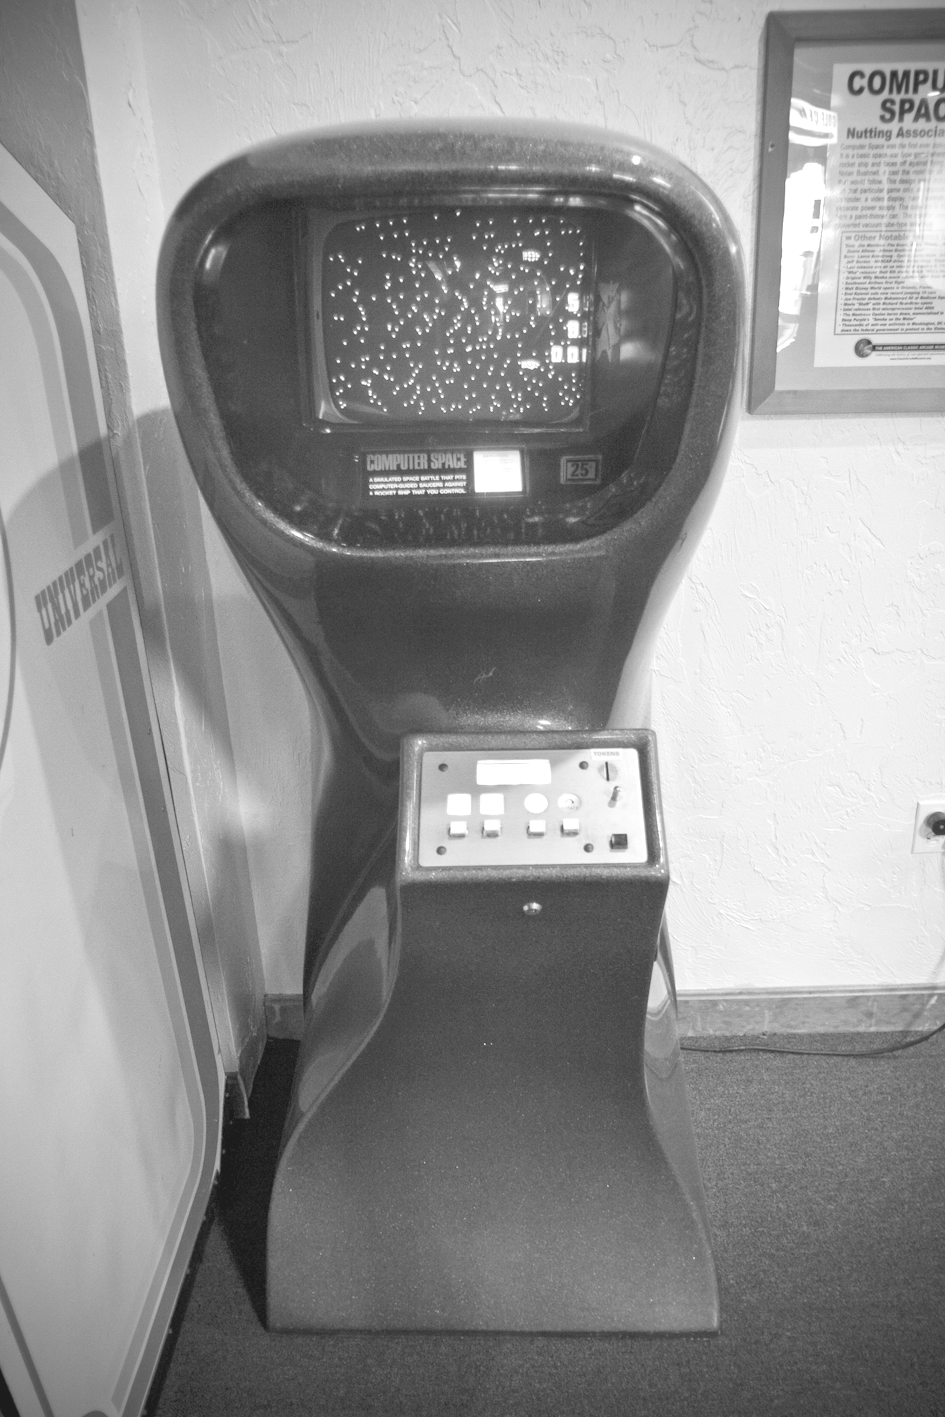
\includegraphics[scale=0.6]{Zcontrib_DJaouti/Djaouti_Computer_Space_Print.png}
\caption{\textit{Computer Space}, un jeu vidéo commercial et propriétaire largement inspiré par \textit{Spacewar!}. (Par Rob Boudon, sous licence Creative Commons -By 2.0.)}
\end{figure}

Mais la plus grande influence de \textit{Spacewar!} sur l'histoire du jeu
vidéo découle directement de l'énorme impression qu'a eu ce titre sur
un étudiant du nom de Nolan Bushnell. Ce dernier est tellement marqué
par le jeu qu'il copie également son concept pour créer la première
borne d'arcade largement commercialisée, \textit{Computer Space} (1971). En effet \textit{Galaxy Game} tourne sur un matériel proche
de celui de \textit{Spacewar!}, dont les
coûts de fabrication l'ont empêché d'être produit à grande échelle.
Pour \textit{Computer Space}, Bushnell recrée
donc le jeu sur du matériel moins onéreux, mais se voit contraint de le
simplifier au passage. Il retire par exemple l'étoile centrale et son
champ de gravité, mais rajoute un mode monojoueur. Le principe du jeu
consiste maintenant à diriger une fusée pour tirer sur des soucoupes
volantes sans se faire toucher. Une seconde version de la borne propose
un nouveau mode de jeu dans lequel les soucoupes volantes peuvent êtres
dirigées par un deuxième joueur. Mais malgré les espoirs du jeune
entrepreneur, la borne, qui est commercialisée en novembre 1971, est un
échec commercial. Pourtant, Bushnell croit en l'idée de commercialiser
des jeux vidéo, sous forme de logiciels et machines propriétaires, au
grand public. Il persévère et fonde, avec son associé Ted Dabney, la
société Atari en juin~1972. Inspiré
par une présentation de la \textit{Magnavox
Odyssey}\footnote{La Magnavox Odyssey est
la première console de jeu vidéo de salon commercialisée auprès du
grand public, tout du moins aux États-Unis. Inventée par Ralph Baer, il
s'agit d'un appareil qui peut se brancher sur un téléviseur afin de
jouer à différents jeux vidéo simples, grâce à deux manettes reliées à
l'appareil. Véritable innovation technologique à l'époque, parmi les
jeux qu'elle propose se trouve un certain «~Ping-Pong~». Il permet à
deux joueurs de s'affronter dans un jeu où il faut renvoyer une balle
en contrôlant des raquettes rectangulaires. Avant sa commercialisation,
la console fut présentée au public. En mai~1972, Bushnell a assisté à
la présentation de l'Odyssey, soit un mois avant qu'il ne fonde la
société Atari et ne définisse le concept du jeu Pong. Si Pong et
Ping-Pong ne se sont pas en tout points identiques
 (par exemple Ping-Pong ne possède pas
de score et n'utilise pas un déplacement limité à l'axe vertical comme
Pong), force est de constater que les deux jeux se ressemblent
beaucoup… Magnavox portera d'ailleurs plainte contre Atari à ce sujet
dès~1974.}, Bushnell invente un nouveau concept de jeu, dont il
confiera la réalisation au premier employé
d'Atari, Alan Alcorn. Ce
nouveau jeu d'arcade, baptisé \textit{Pong} (1972), connaît alors un succès retentissant avec près de 350~000
unités vendues. Créée en~1972, la société
Atari affiche déjà 11~millions de
dollars de chiffre d'affaires en~1973, et plus de 36~millions en~1975\footnote{\cite{learmonthno1999}.}. À ce titre, bien qu'il ne soit pas le premier jeu
vidéo, ni le premier jeu d'arcade, et que son principe fut visiblement
inspiré du jeu  \textit{Ping-Pong} de la \textit{Magnavox Odyssey},
\textit{Pong} est généralement considéré
comme le point de départ de l'industrie du jeu vidéo\footnote{\cite{donovanreplay:2010}.}.
En effet, il est le premier jeu vidéo à avoir connu un véritable succès
commercial de masse. Tout cela serait-il arrivé si Bushnell n'avait pas
autant joué à \textit{Spacewar!} alors qu'il
était étudiant ? On peut légitimement en douter. Mais l'entrepreneur
aurait-il été en mesure de jouer à \textit{Spacewar!} si ce jeu n'avait été pas
été créé selon une philosophie permettant sa libre diffusion ? Après
tout, Bushnell était étudiant à l'université de l'Utah, située à plus
de 4~000~kilomètres du MIT. Comme nous l'avons vu, le fait que \textit{Spacewar!} soit un logiciel ouvert,
préfigurant ainsi les logiciels libres actuels, a grandement participé
à sa large diffusion, que ce soit entre étudiants ou par le biais du
constructeur \textit{DEC}. De plus, Bushnell
aurait-il été en mesure de programmer son jeu \textit{Computer~Space} s'il n'avait pas pu
préalablement étudier le code source de \textit{Spacewar!} ? En d'autres termes,
aurait-il tout simplement pu créer lui-même un jeu vidéo si
\textit{Spacewar!} avait été un logiciel propriétaire ?


En guise de réponse, nous pouvons nous référer une célèbre citation de
Bushnell, qui laisse deviner que l'ouverture des codes sources et la
libre distribution des premiers jeux vidéo l'ont clairement aidé à
donner naissance à une industrie aujourd'hui florissante : «~Je n'ai
pas inventé les jeux vidéo. Ils ont été inventés sur des ordinateurs à
7~millions de dollars. Moi, je n'ai fait que les
commercialiser.~»\footnote{Nous traduisons. \cite{learmonthno1999}.}



\section*{2.~~~Du \textup{shareware} au \textup{modding}}
\phantomsection
\addcontentsline{toc}{section}{2. Du \textup{shareware} au \textup{modding}}

\subsection*{2.1~~~Le \textit{shareware~}: libérer les canaux de distributions de jeux vidéo}
\phantomsection
\addcontentsline{toc}{subsection}{2.1 Le \textit{shareware~}: libérer les canaux de distributions de jeux vidéo}



Attirées par l'incroyable succès de Bushnell et sa société
 Atari, de nombreuses autres
entreprises s'intéressent au jeu vidéo, et proposent des jeux et des
machines de plus en plus sophistiqués. Au-delà de l'innovation
technologique et artistique, le passage des premiers jeux vidéo
commercialisés en~1972 au secteur industriel générant aujourd'hui un
chiffre d'affaires estimé à plusieurs milliards de
dollars\footnote{Voir \url{http://www.afjv.com/news/839_sales-video-game-content.htm}.} s'est également accompagné de la disparition
progressive de toute trace de la philosophie du Libre qui animait les
créateurs de \textit{Spacewar!}. La
commercialisation des logiciels de jeu, qu'il s'agisse de cartouches de
jeu pour ordinateur ou console de salon, ou bien de bornes d'arcade, a
été synonyme de la fermeture de l'accès à leur code source. De même, la
liberté d'exécution s'est trouvée limitée par le fait de ne pouvoir
utiliser certains logiciels de jeu que sur certaines machines. Si
 Atari a tracé les principales lignes
de ce modèle économique reposant sur une logique propriétaire, il n'en
a pas été le seul artisan\footnote{\cite{kentultimate2001}.}. En effet, lors de la sortie de
sa première console de jeu vidéo de salon, la
\textit{VCS~2600} (1977), Atari pensait logiquement qu'il
serait le seul à développer des jeux pour sa machine. Quelle ne fut pas
alors sa surprise de constater que d'autres sociétés, attirées par le
succès commercial de la console, ont –~elles aussi~– commencé à
fabriquer des cartouches de jeu, et ce sans autorisation de la part
d'Atari. La société qui a ouvert la
brèche s'appelle Activision, un
studio indépendant de création de jeu vidéo fondé par quatre
ex-employés d'Atari. Malgré les
protestations d'Atari, la pratique
fut déclarée légale car Activision n'enfreignait aucun brevet propre à Atari. Cette «~erreur~» fut réparée
par  Nintendo lors de la génération
suivante de consoles. En effet, les cartouches de jeux pour la console
\textit{Nintendo NES} (1983) embarquent une
puce de protection, la \textit{10NES}\footnote{Voir
\url{http://en.wikipedia.org/wiki/10NES} pour plus de détails}. Cette
puce, au code breveté, garantit que seul Nintendo peut légalement produire
des cartouches de jeu pour sa console. Ce faisant, l'industrie du jeu
vidéo a réussi à non seulement limiter la liberté des utilisateurs de
logiciels, mais aussi celle des créateurs. Cette politique est toujours
d'actualité aujourd'hui, où les créateurs de jeu vidéo doivent recevoir
une autorisation (payante) de la part des constructeurs de consoles de
jeu afin de pouvoir développer dessus. Un modèle similaire se poursuit
avec certains circuits de distributions dématérialisés. Par exemple, le
\textit{Xbox Live Arcade} dont les portes
d'entrées sont contrôlées par Microsoft, ou encore Steam dont seul le propriétaire, Valve, peut autoriser un jeu à y
figurer. Enfin, si le développement de jeux vidéo sur ordinateur a de
tout temps été accessible à toute personne possédant des connaissances
techniques en la matière, le fait d'éditer, fabriquer et commercialiser
un jeu dans un réseau de magasins physiques représente depuis la fin
des années~1980 un coût de plus en plus important\footnote{D'après
des données américaines datant de~2010, la moitié du prix d'un jeu
vendu en magasin est consacrée à sa distribution, l'autre moitié
couvrant les coûts de développement et de marketing :
\url{http://latimesblogs.latimes.com/entertainmentnewsbuzz/2010/02/anatomy-of-a-60-dollar-video-game.html}.}. Cela limite donc considérablement la possibilité
pour tout créateur de jeu vidéo indépendant d'y distribuer ses
réalisations.

D'autres circuits de distribution se mettent alors en place pour
permettre une distribution plus libre de jeux vidéo. Optant pour la
distribution de logiciels sous forme dématérialisée, ces circuits de
distribution parallèles s'appuient tout d'abord sur des serveurs
BBS\footnote{Un Bulletin Board System est un ordinateur auquel d'autres
ordinateurs peuvent se connecter par le biais d'un modem. Une fois
connecté à un BBS par le réseau téléphonique, un utilisateur peut
discuter avec d'autres membres, envoyer ou récupérer des fichiers,
jouer à des jeux en réseau… Il s'agit en quelque sorte de l'ancêtre
d'Internet et de ses nombreux services. Les BBS rencontreront un
certain succès auprès des passionnés d'informatique, à une époque où le
«~réseau des réseaux~» n'était pas encore accessible au grand public
(soit de la fin des années~1970 au milieu des années~1990).}, puis sur
Internet. Deux principaux types de logiciels circulent sur ces réseaux.
D'un coté les \textit{freeware}, logiciels intégralement gratuits, et de
l'autre les \textit{shareware}, dont une version incomplète est distribuée
gratuitement dans l'espoir que vous en commandiez la version complète
et payante directement au créateur. Si tous les types d'applications se
retrouvent sur ces réseaux, les jeux vidéo y sont largement
représentés. Par rapport aux autres circuits de distribution de jeux
vidéo, les réseaux BBS et Internet sont relativement «~libres~», car
tout le monde ou presque peut y distribuer ses créations. Cette liberté
permet donc enfin à des jeux vidéo optant pour une philosophie
différente du modèle propriétaire d'exister. Certains jeux vidéo de
type \textit{freeware} sont alors parfois distribués avec leur code
source sur ces réseaux, même si cela n'est pas la norme\footnote{Par
exemple, sur les 777~jeux vidéo indépendants référencés sur
\url{http://db.tigsource.com/}, seulement 8 sont distribués avec leur
code source. Cela représente uniquement 1~\% des titres de cette base
de données recensant des jeux vidéo distribués exclusivement par voie
dématérialisée.}. 

Dans les années~1980, au-delà du développement des réseaux
informatiques, nous assistons également à la formalisation des
pratiques d'ouverture de code source et de libre distribution de
logiciels sous forme de licences juridiques. Nous pouvons par exemple
penser à la célèbre licence GNU/GPL, dont la première version
officielle est publiée en~1989, ou aux premières versions de la BSD
licence qui remontent à~1988. Si le courant du logiciel libre associe
l'ouverture de code source à une éthique prônant le partage et la libre
distribution, le courant de l'Open-source, apparu quelques années plus
tard, s'arrête quant à lui au seul fait que le code source d'un
logiciel soit ouvert\footnote{Pour plus de détails à ce sujet, voir
par exemple \url{http://fr.wikipedia.org/wiki/Logiciel_libre}.}. Ainsi,
qu'ils soient présentés comme logiciels libres, comme Open-source, ou
qu'il s'agisse tout simplement d'un programme au code source ouvert
publié avant toute formalisation d'une philosophie du Libre, de
nombreux jeux vidéo ont pu être diffusés sur les réseaux BBS et
Internet depuis la fin des années~1970 jusqu'à nos jours. Mais ces
modes de distribution électronique n'ont pas uniquement contribué au
retour des jeux vidéo ouverts sous la forme de logiciels libres ou
Open-source. Ils ont également largement contribué au développement du
piratage de logiciels, phénomène qui n'a bien évidemment pas épargné
les jeux vidéo. Cette thématique sort du cadre de ce chapitre, mais
notons néanmoins que dès le début des années~1980, les réseaux BBS puis
Internet ont permis à des groupes de crackers de distribuer
gratuitement des jeux vidéo commerciaux débarrassés de tout dispositif
technique de protection contre la copie. Si les motivations des
crackers pour s'investir dans une telle activité, de nature illégale
dans la plupart des pays, sont nombreuses et variées, le fait de
«~libérer des logiciels propriétaires~» en fait généralement partie\footnote{\cite{craigsoftware2005}.}.


En résumé, l'apparition de nouveaux modes de distribution a tout d'abord
contribué au retour des jeux vidéo ouverts, qui rejoignent ensuite les
rangs du logiciel libre ou des logiciels Open-source avec la
formalisation de ces philosophies. Mais ces réseaux ont également
permis l'apparition du piratage des nombreux jeux vidéo reposant
toujours sur le modèle du logiciel propriétaire. En effet, malgré
l'apparition des BBS et d'Internet, le logiciel propriétaire reste le
modèle de référence du jeu vidéo depuis les prémices commerciaux de son
industrie. Cependant, au-delà de ces deux impacts majeurs, les réseaux
BBS et Internet aident également à ré-insuffler un peu de la
philosophie de partage et de création collaborative chère au Libre au
sein des jeux vidéo, en particulier du coté des shareware\footnote{Le
\textit{shareware}, ou «~partagiciel~», désigne un mode de distribution de
logiciels qui consiste à diffuser gratuitement une version
fonctionnelle mais limitée de son programme pour donner envie à
l'utilisateur d'en acheter une version complète. Dans le cas du jeu
vidéo, il s'agit de titres, par exemple \textit{Doom} (id Software,
1993), dont les premiers niveaux sont diffusés gratuitement, le joueur
devant ensuite acheter les niveaux suivants directement aux créateurs
du jeu.} avec l'apparition de la pratique du \textit{modding}.




\subsection*{2.2~~~Le modding}
\phantomsection
\addcontentsline{toc}{subsection}{2.2 Le modding}

Comme son nom l'indique, la notion de\textit{modding} désigne le fait de modifier
un jeu existant, pour ensuite redistribuer le fruit de ce travail. Le
résultat du \textit{modding} est tout
simplement baptisé un \textit{mod}. Mais
contrairement à un logiciel libre dont on modifierait directement le
code source pour ensuite redistribuer librement la version modifiée, un \textit{mod} n'est pas autonome. Un \textit{mod} ne contient qu'un ensemble de
modifications effectuées sur un jeu donné. La possession du jeu
originel est donc requise pour jouer à un \textit{mod}. Qu'est-ce qui peut donc
justifier un principe de fonctionnement aussi complexe ?


Tout simplement le fait que, contrairement aux logiciels libres, les
jeux vidéo pour lesquels sont créés des \textit{mods} sont généralement des logiciels
propriétaires et commerciaux. Concrètement, les
 \textit{mods} créés ne peuvent être
commercialisés et sont parfois de nature Open-source, mais pour pouvoir
jouer à un \textit{mod} donné il faut
auparavant acheter un jeu vidéo commercial et propriétaire. Prenons
pour exemple le jeu vidéo de type \textit{mod} le plus connu, à savoir \textit{Counter-Strike} (Minh Le \& Jess Cliffe, 1999). Ce jeu de tir en vue subjective a été le jeu vidéo
multijoueur le plus pratiqué sur Internet pendant la première moitié
des années~2000\footnote{D'après
\url{http://store.steampowered.com/stats/}.}.
Distribué gratuitement par le biais d'Internet, son installation
nécessite d'avoir au préalable acheté et installé le jeu \textit{Half-Life} (Valve, 1998), le jeu d'origine à partir duquel \textit{Counter-Strike} a été créé. Si \textit{Counter-Strike} a été réalisé par des
amateurs éclairés sur leur temps libre, \textit{Half-life} est par contre la création
d'un studio de développement professionnel. Si les créateurs de \textit{Half-life} autorisent ainsi tout amateur à créer et redistribuer librement des variantes de leur jeu,
c'est parce que l'utilisation de ces variantes s'accompagne
obligatoirement de l'achat du jeu originel. Ceci explique pourquoi les
créateurs de \textit{Half-life} ont, sur le
cédérom de leur jeu, inclut des versions simplifiées des outils qu'ils
ont utilisés lors de son développement. En distribuant ainsi leurs
outils de travail, ils encouragent explicitement les amateurs à créer
des variantes de leur propre jeu, qui seront ensuite distribuées sous
forme de \textit{mods}. Au final, si
l'industrie du logiciel utilitaire arrive à faire cohabiter Libre et
activité commerciale à travers la vente de services (formation, support), il semble que
l'industrie du jeu vidéo a de son côté trouvé une autre voie à travers
la pratique du \textit{modding}.
Philosophiquement, nous retrouvons dans ce modèle les idées de partage
et d'amélioration de logiciels propre au logiciel libre, idées qui
semblent avoir quitté l'industrie du jeu vidéo après \textit{Spacewar!}. Alors, comment un
développeur de jeux vidéo commerciaux et propriétaires aurait-il pu
avoir un jour l'idée «~folle~» de distribuer librement ses outils de
travail afin d'autoriser n'importe qui à bidouiller ses propres
créations ?

\subsection*{2.3~~~Le \textit{shareware} comme berceau du \textit{modding}}
\phantomsection
\addcontentsline{toc}{subsection}{2.3 Le \textit{shareware} comme berceau du \textit{modding}}

La réponse à cette question se trouve parfaitement illustrée par
l'histoire d'un jeu vidéo en particulier, distribué sous forme de
\textit{shareware~}: \textit{Doom}(id Software, 1993). Il s'agit d'un jeu de tir en vue subjective, qui a
marqué l'histoire du jeu vidéo en définissant les codes de ce genre
vidéoludique aujourd'hui très populaire. La société à l'origine de
 \textit{Doom},
\textit{id Software}, est un petit studio
indépendant dont les créations sont exclusivement distribuées sur
serveur BBS selon les modalités du «~shareware~». Tout commence lors de
la publication de leur jeu
\textit{Wolfenstein~3D} (id Software, 1992).
Les créateurs d'id Software furent
très surpris de constater que de nombreux joueurs créaient de nouveaux
niveaux et des versions modifiées de ce titre, qu'ils s'échangeaient
ensuite librement sur BBS\footnote{\cite{kushnermasters2004}.}. Mais id Software ne chercha pas à réprimander ces joueurs qui avaient, en toute illégalité, «~hacké~»
leur création afin de pouvoir la modifier. Au contraire, la société
chercha à encourager (et quelque part à encadrer) cette pratique pour
leur prochain titre, alors en cours de réalisation : \textit{Doom}. 


Ainsi, le programmeur du jeu, John Carmack, a inventé le format de
fichier \textit{WAD}\footnote{Acronyme
de \textit{Where's All the Data?}.}, afin de
séparer le «~contenu~» du jeu de son «~moteur~». Cela permet dorénavant
aux joueurs de créer facilement du nouveau contenu pour \textit{Doom} sans avoir à hacker le jeu. Il s'agit là d'un des premiers exemples de légitimation de la pratique
visant à la modification de jeux vidéo commerciaux par des amateurs,
par la suite appelée \textit{modding}. Mais
cette légitimation ne s'est pas faite sans contrepartie. En effet, id Software demanda explicitement à
ce que le contenu créé par les joueurs ne puisse fonctionner que sur la
version complète et payante du jeu, et non sur la version de
démonstration gratuite (principe du \textit{shareware}). Le hasard fit que
la sortie de ce titre, qui rencontrait déjà un certain succès critique
et commercial, s'accompagnait du développement d'Internet pour le grand
public. Ainsi, les amateurs qui créaient de nouveaux niveaux, monstres,
armes et autres variantes de \textit{Doom}
pouvaient se les échanger à travers des sites de fans tels que \textit{Doomworld} (1993-2012) et \textit{Gamers.org-DoomGate} (1994-2012). 
Pourtant,id Software ne livra pas
ses outils de développement avec \textit{Doom}, bien qu'elle encourageât les
joueurs à modifier son titre. En effet, l'éditeur de niveaux utilisé
pour créer \textit{Doom} ne tourne que sur PC (Ms-Dos). Les outils de
développement n'étant pas accessibles aux joueurs pour de simples
questions techniques, ceux-ci s'empressèrent de créer de nombreux
outils par eux-mêmes. Par exemple, \textit{Doom Editing Utility} (Brendon Wyber,
1994), diffusé un mois seulement après la sortie du jeu, permet d'en
modifier les niveaux, tandis que \textit{DeHacked} (Greg Lewis, 1994), sert à
en altérer les règles.


\begin{figure}
\centering
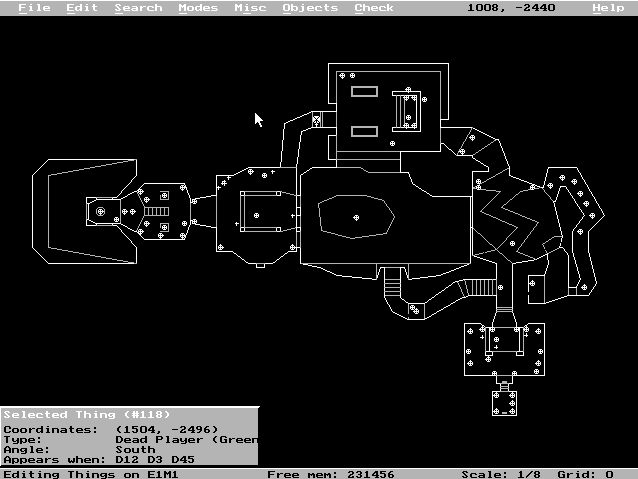
\includegraphics[scale=0.4]{Zcontrib_DJaouti/Djaouti_DoomEditingUtility.png}
\caption{\textit{Doom Editing Utility}, le premier éditeur de niveau pour  \textit{Doom} accessible à tous.} 
\end{figure}

Il faut ensuite attendre la sortie de \textit{Duke Nukem 3D} (3D Realms, 1996) pour
qu'un développeur livre directement tous ses outils de développement
avec le jeu. D'après Scott Miller, un des créateurs de
\textit{Duke Nukem 3D}, cette décision était
courageuse à une époque où l'industrie du jeu vidéo pensait qu'il ne
fallait absolument pas diffuser ses outils et
technologies\footnote{D'après une interview personnelle de Scott
Miller réalisée par mail en mai~2010}. L'histoire montre qu'à
l'inverse, cette pratique augmente le potentiel commercial du jeu en
prolongeant sa durée de vie. Ainsi, plus de quinze~ans après sa sortie,
\textit{Doom} est toujours joué et utilisé
comme support de création. De nouveaux éditeurs de niveaux continuent
même à voir le jour pour ce titre, à l'image
\textit{Doom Builder~2} (Pascal vd Heiden,
2009). Quelques années plus tard,
\textit{Counter-Strike} semble être le
premier \textit{mod} dont le succès populaire
dépasse largement celui de son jeu d'origine. Ce succès permet au grand
public de découvrir la pratique du
\textit{modding}, qui restait jusqu'alors
cantonnée à une certaine frange de joueurs passionnés\footnote{\cite{laukkanenmodding2005}.}. Aujourd'hui, la création de
\textit{mods} représente une valeur marchande
indirecte pour les éditeurs de jeux vidéo\footnote{\cite{postigomods2007}.}, à tel point
que certains professionnels de l'industrie intègrent dorénavant la
création amateur de \textit{mods} dans leur
stratégie commerciale\footnote{\cite{nieborgmod2008}.}.

\section*{3.~~~La création amateur de jeu vidéo : de l'Open source au Jeu 2.0}
\phantomsection
\addcontentsline{toc}{section}{3. La création amateur de jeu vidéo : de l'Open source au Jeu 2.0}


En parallèle à l'histoire du jeu vidéo commercial, et de l'industrie
qu'il fait vivre, la création de jeu vidéo est également pratiquée en
amateur depuis de nombreuses années. Comme nous allons le voir,
l'influence du Libre sur la création vidéoludique amateur est assez
différente de celle que nous venons d'étudier du coté des industriels
du jeu vidéo. 

\subsection*{3.1~~~L'échange de code source}
\phantomsection
\addcontentsline{toc}{subsection}{3.1 L'échange de code source}

L'histoire de la création de jeu vidéo en amateur est intimement liée à
celle de l'informatique, en particulier au développement de la
micro-informatique personnelle\footnote{\cite{chaplinsmartbomb2005}.}. Un des premiers
micro-ordinateurs à avoir rencontré un succès commercial auprès du
grand public est l'\textit{Altair~8800} (MITS, 1975). Sorti en~1975, cet ordinateur avait la particularité
d'être vendu en kit. Il a donc rapproché de nombreux passionnés
d'informatique, qui se sont rapidement regroupés au sein de «~clubs~»
afin d'échanger des conseils d'assemblage. Mais ces clubs étaient aussi
un excellent moyen d'échanger des programmes pour cette
machine. L'un des rares programmes
disponibles lors de sa sortie était
l'\textit{Altair Basic} (Micro-Soft, 1975),
première création commerciale d'une jeune société qui sera plus tard
connue sous le nom de Microsoft. Les
détenteurs d'un \textit{Altair~8800} pouvaient donc écrire leurs propres programmes en langage BASIC. Si
seuls certains de ces clubs deviendront célèbres, à l'image du Homebrew Computer Club fréquenté par
Steve Jobs et Steve Wozniak, tous avaient la particularité de permettre
la circulation de nombreux petits jeux vidéo écrit en BASIC\footnote{\cite{wolfvideo2007}.}. Réalisés par des amateurs, ces jeux vidéo s'échangeaient
directement sous forme de listing BASIC. Cette pratique informelle a
rapidement été accompagnée par la publication d'ouvrages regroupant des
codes sources de jeux en BASIC, tel que
\textit{Basic Computer Games}\footnote{\cite{ahlbasic1978}}. 
Écrit par le journaliste et spécialiste de l'histoire du jeu vidéo
David Ahl, cet ouvrage rassemble les codes sources de 101~jeux. Il a
connu plusieurs éditions pour diverses machines. La première date
de~1973 et est consacrée au BASIC tournant sur les ordinateurs de la
famille \textit{PDP} du constructeur DEC. La version de~1978, consacrée
au BASIC de Microsoft, rencontra un
énorme succès auprès du public puisque plus d'un million d'exemplaires
furent vendus au total. L'ouvrage fut même traduit en français par Sybex en~1980. À noter que
l'année~2010 vit une réédition de cet ouvrage pour le langage
Smallbasic\footnote{\url{http://smallbasiccomputergames.com/}.}. Au fur et à mesure de la sortie de nouveaux modèles de
micro-ordinateurs de plus en plus performants, tels que
l'\textit{Apple~II} (Apple, 1977), la
création et l'échange de jeux amateurs sous forme de codes sources se
développa considérablement. Certains magazines se spécialisèrent même
dans cette activité, à l'image du français
\textit{Hebdogiciel} (Shift Éditions, 1983-1987). 


Cependant, à partir de la fin des années~1970, la plupart des
micro-ordinateurs étaient équipés d'un lecteur de disquettes ou de
cassettes. Cela permettait donc également aux amateurs d'échanger leurs
créations vidéoludiques directement sous forme électronique. Le fait de
ne plus être obligé de partager le code source pour diffuser leurs
créations semble avoir détourné de nombreux amateurs de la voie du
Libre. Si la création de jeux amateurs en Open-source restait bien
évidemment populaire, elle n'était plus la seule voie possible. Mais la
diffusion de jeux amateurs directement sous forme logicielle amène une
nouvelle problématique. En effet, même avec le langage BASIC, la
création de jeux vidéo reste une tâche relativement complexe, en
particulier pour des débutants. Certains membres des communautés
amateurs ont donc imaginé des outils destinés à simplifier la création
de jeu vidéo : les «~usines à jeux~».

\subsection*{3.2~~~Les usines à jeux}
\phantomsection
\addcontentsline{toc}{subsection}{3.2 Les usines à jeux}

Devant la complexité que représente la réalisation d'un nouveau jeu
vidéo pour des amateurs, certains programmeurs ont imaginé des outils
logiciels permettant de faciliter leur création. Le plus ancien que
nous ayons pu recenser à ce jour est
\textit{Eamon} (Brown, 1980). Explicitement
destiné à une diffusion non commerciale, ce programme est un jeu de
rôle et d'aventure en mode texte, dans la grande tradition de
\textit{Colossal Cave Adventure} (Crowther \& Woods, 1976). Mais surtout, il est livré avec des utilitaires
permettant de créer ses propres aventures, qui sont ensuite
redistribuables sous forme de jeux autonomes\footnote{\cite{kunzebrief2008}.}. Il
s'agit là d'un exemple de programme destiné à simplifier la création de
nouveaux jeux vidéo, de manière à la rendre accessible à des
non-programmeurs. Ce genre d'outil logiciel s'est considérablement
développé par la suite, structurant la sphère des créateurs amateurs en
«~communautés~» centrées sur un logiciel donné. Nous appelons de tels
logiciels des «~usines à jeux~», que nous pouvons définir comme un
logiciel «~tout-en-un~» permettant de créer un jeu vidéo autonome sans
forcément partir d'une base existante. La notion «~d'usine~» se
justifie par l'idée d'avoir un logiciel «~tout-en-un~», centralisant
donc ainsi une chaîne de production complète de jeux vidéo. Bien que
principalement utilisés par les amateurs, des outils similaires sont
aussi utilisés dans l'industrie à des fins de réduction de coûts de
production par économie d'échelle.

Après \textit{Eamon}, d'autres usines à jeux
sont rapidement apparues pour proposer de créer d'autres genres de
jeux. Ces jeux s'appuient d'ailleurs sur une représentation graphique
et sonore plus évoluée : des graphismes en~2D au lieu du texte. L'outil
le plus emblématique est sans doute
\textit{Pinball Construction Set} (Budge, 1983). Comme son nom l'indique, ce logiciel pionnier permet de créer
des jeux de flipper. Les divers éditeurs du logiciel permettent de
composer une table de flipper en posant divers éléments (bumpers,
trous…), puis d'en définir les règles de bases (nombre de balles…). Le
jeu est ensuite exportable sous forme autonome, ce qui permet de le
diffuser librement. Le succès critique et commercial rencontré par cet
outil a inspiré la création de nombreux logiciels similaires, toujours
destinés à la création d'un genre vidéoludique en particulier\footnote{\cite{bartonhistory2010}.}. Par exemple,
\textit{Adventure Construction Set} (Smith,
1984) permet de réaliser des jeux de rôle et d'aventure dans la veine
des premiers opus de la série \textit{Ultima} (Garriot, 1980-2009). De son côté, \textit{
Racing Destruction Set} (Koenig, 1985) permet de créer des jeux de
course, alors que \textit{Wargame Construction Set} (Strategic Simulations Inc, 1986) se focalise sur les jeux de
stratégie militaire au tour par tour. Si toutes ces usines à jeux sont
spécialisées dans la création d'un genre de jeu en particulier, il en
existe également d'autres qui permettent de créer tous les genres
vidéoludique, voire d'en inventer de nouveaux. Le pionnier en la
matière est sans conteste \textit{Gamemaker} (Kitchen, 1985), qui fut ensuite suivi par deux familles de logiciels
aujourd'hui très populaires. D'un coté, les logiciels créés par la
société Clickteam, qui rassemblent notamment \textit{Klik \& Play} (1994),
\textit{The Games Factory} (1998) ou encore \textit{Multimedia Fusion~2} (2006). De
l'autre, les différentes versions de
\textit{Game~Maker} (Overmars, 1999-2012).
Ces deux familles d'outils sont destinées à la création de jeux vidéo
en 2D. Mais nous pouvons également citer la gamme des
\textit{3D Game Studio} (Conitec, 1993-2010),
\textit{BlitzMax} (Blitz Research, 2004) ou encore les différentes
versions d'\textit{Alice} (Pausch \& al., 1995-2010) qui permettent la création de jeux vidéo en~3D. La place
nous manque pour rentrer dans le détail historique des très nombreuses
usines à jeux existantes. Nous renvoyons donc le lecteur intéressé par
le sujet au site \textit{Game Creation Tools Classification} \footnote{\url{http://creatools.gameclassification.com}.},
une base de donnée collaborative en ligne qui recense plus de
450~usines à jeux publiées depuis~1980.


Cependant, qu'elles soient disponibles gratuitement ou diffusées
commercialement, force est de constater que la plupart des usines à
jeux sont des logiciels propriétaires. Cela peut paraître regrettable
car, comme c'est le cas des jeux commerciaux permettant le
\textit{modding}, l'ouverture du code source d'une usine à jeux semble prolonger sa durée
de vie. C'est par exemple le cas de
\textit{MegaZeux} (Janson, 1994), destiné à
faciliter la création de jeux d'action-aventure utilisant des
graphismes ASCII\footnote{Acronyme de
American Standard Code for Information Interchange. Il s'agit d'une norme
informatique pour l'encodage des caractères. Avant l'apparition de
moteurs graphiques performants, il était possible de détourner les
fonctions d'affichage textuel d'un ordinateur pour simuler des dessins,
en utilisant notamment les caractères spéciaux définis dans la norme~ASCII.}.
Originellement diffusé sous forme de \textit{shareware} en~1994, la carrière de
cette usine à jeux fut prolongée par son passage dans le domaine public
en~1999. Le développement de
\textit{MegaZeux} a alors été poursuivi par
une communauté d'amateurs passionnés. Aujourd'hui, de nombreux jeux
continuent à être créés avec
\textit{MegaZeux}, grâce une communauté
d'utilisateurs restreinte mais toujours active plus de quinze ans après
la sortie du logiciel. \textit{Official
Hamster Republic Role Playing Game Creation Engine} (Paige, 1997) a
connu un destin similaire. D'un logiciel payant, il est devenu un
logiciel gratuit avant d'atteindre le statut Open-source. Il continue
ainsi a être régulièrement mis à jour, ayant déjà permis à ses
utilisateurs de créer plusieurs centaines de jeux de rôle et d'aventure
en~2D. Plus récemment, nous pouvons penser à
\textit{Open Beats of Rage} (Lavalit Team, 2012), spécialisé dans la création des jeux de combats. Ce logiciel est
basé sur \textit{Beats of Rage} (Senile Team,
2003), qui fut abandonné par ses concepteurs au bout de quelques
années. Ces derniers ont alors accepté d'en ouvrir le code source,
permettant à une communauté de développeurs adeptes de la philosophie
du Libre de continuer à le faire évoluer. 

\begin{figure}
\centering
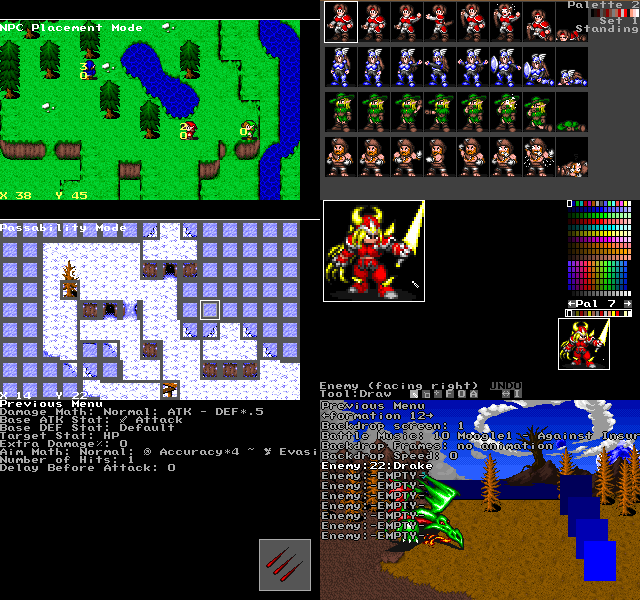
\includegraphics[scale=0.4]{Zcontrib_DJaouti/Djaouti_OHRRPGCE.png}
\caption{\textit{Official Hamster Republic Role Playing Game Creation Engine} est une usine à jeux qui, en passant du statut de logiciel propriétaire à l'\textit{open-source}, a gagnée en popularité et longévité. (Par Bob the Hamster, GNU GPL}
\end{figure}

Bien qu'intéressants, ces exemples d'usines à jeux distribuées sous
forme de logiciels libres sont l'exception qui confirment la règle :
les outils destinés à faciliter la création de jeu vidéo par des
amateurs sont généralement des logiciels propriétaires\footnote{Sur
les 452~logiciels référencés sur la base de données
\url{http://creatools.gameclassification.com}, seuls 81~outils sont
des logiciels libres, soit environ 18~\% des usines à jeux référencées
sur cette base de données.}. Mais si les concepteurs d'usines à jeux ne
sont pas forcément adeptes du Libre, la situation semble être
différente pour certains de leurs utilisateurs. À la manière des
«~clubs~» qui permettaient l'échange de jeux amateurs sous forme de
code source, de nombreux utilisateurs d'usines à jeux se structurent en
«~communauté de créateurs~» dédiées à un logiciel donné par le biais
d'Internet. Par exemple, le site \textit{The
Daily Click} (2002-2012) est dédié aux usines à jeux créés par la
société Clickteam, tandis que
\textit{Game Maker Games} (2004-2012) est
centré sur les différentes versions de
\textit{Game Maker}. Si les jeux échangés sur
ces sites sont généralement «~protégés~» afin que leur code source ne
soit pas accessible, nombre d'entre eux sont également diffusés sous
forme \textit{open source}. Cela permet d'aider les débutants dans leur
apprentissage, ou encore de donner la possibilité aux membres d'une
communauté de tenter d'améliorer un jeu vidéo créé par d'autres
amateurs. Cette pratique informelle et spontanée de la part des
utilisateurs d'usines à jeux existe depuis
\textit{Eamon}, grâce à des communautés
basées sur des serveurs BBS ou des sites Internet. Cependant, certains
créateurs d'usines à jeux ont également tenté de légitimer et
d'encourager cette pratique à travers le courant du
\textit{Jeu 2.0}. 

\subsection*{3.3~~~Le «~Jeu 2.0~»}
\phantomsection
\addcontentsline{toc}{subsection}{3.3 Le «~Jeu 2.0~»}

Nous pourrions définir simplement le
\textit{Jeu~2.0} comme la rencontre entre des
logiciels de création vidéoludique existants depuis plusieurs années,
les usines à jeux, avec des plateformes de partage inspirées du
\textit{Web~2.0}. Certes, les créateurs de
jeux vidéo amateurs n'ont pas attendu l'arrivée du
\textit{Jeu~2.0} pour partager leurs
créations. Comme évoqué dans la section précédente, de nombreux sites
Internet permettent de diffuser des jeux vidéo amateurs. Mais dans tous
ces exemples, les plateformes de partage ne sont pas intégrées au
logiciel de création. Il faut quitter ce dernier afin d'échanger et/ou
de jouer à ces jeux. L'apport du
\textit{Jeu~2.0} ne se situe donc pas du côté
des capacités de création mais au niveau du «~partage~», à travers la
mise à disposition non pas d'un logiciel, mais d'une véritable
plateforme intégrée qui associe outil de création et fonctionnalités
communautaires. Au sein d'une application unique, il est dorénavant
possible de créer, échanger et jouer à du «~contenu ludique~». 

Le courant du \textit{Jeu~2.0} vise ainsi à
encourager les expériences collaboratives de création vidéoludique. En
facilitant les échanges entre créateurs, un même projet de jeu peut
être conçu par plusieurs personnes différentes. Par exemple, avec
\textit{The Sims Carnival} (Electronic Arts,
2008), tout internaute peut, en
cliquant sur un bouton, modifier un jeu existant sur la plateforme de
partage et en publier une variante. La plateforme de partage gardant
une trace des contributions de chacun, il est possible d'observer des
créateurs qui ne se connaissent pas œuvrer collectivement à la
réalisation d'un même jeu vidéo. Pour cela, il suffit que chaque
créateur travaille à tour de rôle sur la version créée par un des
participants au projet. Dans un registre similaire, chaque partie du
jeu \textit{Spore} (Electronic Arts, 2008)
contient des éléments qui auront été créés par différents joueurs.
Lorsqu'un joueur lance une nouvelle partie, le jeu va récupérer sur la
plateforme d'échange des objets imaginés par d'autres joueurs, tels que
des créatures ou des bâtiments, et les utilise pour construire un monde
unique. S'il le souhaite, le joueur peut même modifier ces créations
provenant d'autres joueurs, avant de les partager à nouveau.

Cependant, cette association profonde entre un logiciel de création
vidéoludique et une plateforme de partage n'est pas sans conséquences.
En effet, si l'éditeur du logiciel «~débranche~» la plateforme de
partage, l'outil de création disparaît avec elle. Or, faire vivre une
plateforme de partage représente un coût financier non négligeable.
Nous pouvons alors comprendre que pour les
\textit{Jeux~2.0} du secteur du
divertissement, la concurrence est très rude. De nombreux outils
risquent de disparaître s'ils ne rencontrent pas le succès escompté par
leur éditeur. Lors d'une étude sur le
\textit{Jeu~2.0} (Djaouti, 2011), nous avions
identifié 31~outils de type \textit{Jeu~2.0}
qui ont été publiés entre~2007 et~2011. Aujourd'hui, 10~de ces outils
ont disparu suite à la fermeture de leur plateforme de partage par
leurs éditeurs respectifs. L'approche du
\textit{Jeu~2.0}, qui vise à pousser les
utilisateurs d'usines à jeux à partager leurs créations selon des
modalités reprenant une partie de la philosophie du Libre, est des plus
intéressantes. Pourtant, il semble qu'un modèle économique adapté au
\textit{Jeu~2.0} reste à trouver. En effet,
les plateformes de partage propres aux
\textit{Jeu~2.0} sont pour l'instant toutes
fournies gracieusement en dépit de leur évident coût de fonctionnement.
Cela explique que de nombreux outils disparaissent, faute de pouvoir
être financés à perte par leur éditeur. Dans l'idéal, un meilleur
modèle économique devrait donc permettre aux plateformes de
\textit{Jeu~2.0} de subsister, voire d'être
profitables, sans pour autant empiéter sur la liberté de création
qu'elles offrent aux utilisateurs. C'est un défi auquel ont fait face
les sites du \textit{Web~2.0}, à l'image de
Wikipédia dont la pérennité repose
en grande partie sur les dons qu'elle reçoit, ou de
Youtube qui s'appuie sur la
diffusion de publicités. L'exemple du
\textit{modding} nous montre que l'industrie
des jeux vidéo a déjà réussi, par le passé, à imaginer un modèle
économique permettant de faire cohabiter son fonctionnement
profondément propriétaire avec la philosophie du Libre. L'histoire se
répètera-t-elle pour le \textit{Jeu~2.0} ?
Face au formidable potentiel de création et de partage que ce courant
représente pour les créateurs amateurs de jeux vidéo, nous ne pouvons
que l'espérer…



\section*{Conclusion}
\phantomsection
\addcontentsline{toc}{section}{Conclusion}

Depuis ses premiers jours, les profits de l'industrie du jeu vidéo
reposent avant tout sur la commercialisation de logiciels
propriétaires, dont l'utilisation et la diffusion sont artificiellement
encadrées afin d'assurer une rentabilité maximale. Pourtant, les jeux
vidéo ne sont pas étrangers à la philosophie du Libre, comme nous le
montrent les trois périodes historiques abordées dans ce chapitre. 

Tout d'abord, l'invention même des jeux vidéo s'est faite dans le cadre
de logiciels au code source ouvert et à la distribution sans entraves,
approches qui seront ensuite formalisées par les courants du logiciel
Libre et de l'Open-source. La création du premier jeu vidéo à avoir une
influence notable, \textit{Spacewar!} (1962), doit d'ailleurs beaucoup à
son statut ouvert, qui préfigure celui des logiciels libres. Comme nous
l'avons évoqué, la première version du jeu n'était pas particulièrement
captivante, et souffrait de nombreux défauts de jouabilité. Le code
source du jeu étant ouvert, ce dernier a pu évoluer de manière
considérable grâce aux ajouts de personnes qui n'étaient pas à
l'origine du projet. Grâce à ces améliorations successives, le jeu est
devenu particulièrement populaire au sein du MIT, l'université
américaine qui l'a vu naître. De plus, l'ouverture de son code source
s'appliquait également à sa diffusion, voulue aussi libre que possible.
Le code source du jeu a donc pu être diffusé vers les diverses
universités américaines, permettant à de nombreux étudiants de
découvrir les jeux vidéo. Influencée par cette première expérience
vidéoludique, et après en avoir étudié le code source, certains
étudiants à l'esprit entrepreneur ont alors eu l'idée de commercialiser
ces «~jeux vidéo~», en les transformant en logiciels propriétaires au
passage.

Pourtant, l'influence de l'esprit du logiciel Libre dans l'histoire du
jeu vidéo ne se limite pas à son commencement, même si c'est la période
où elle a été la plus forte. Face au verrouillage des circuits de
distribution de jeu vidéo par les plus grosses entreprises de
l'industrie vidéoludique, certains créateurs indépendants ont profité
de l'apparition de nouveaux modes de communication plus libres, tels
que les serveurs BBS et Internet, pour diffuser leur œuvres. Ces
circuits de diffusion parallèles, ouverts par nature, pouvaient alors à
nouveau accueillir des jeux Open-source, des jeux propriétaires mais
gratuits (\textit{freeware}) ou encore des jeux commerciaux au modèle
économique singulier (\textit{shareware}). C'est au sein des jeux vidéo
distribués en tant que \textit{shareware}, et plus particulièrement
avec \textit{Doom} (1993), que se développe
un courant associant une pratique du Libre au logiciel propriétaire de
manière originale : le \textit{modding}.
Certains créateurs de jeux vidéo commerciaux diffusent sciemment leurs
outils de développement afin de permettre à quiconque de créer et
diffuser librement des variantes de leur jeu. En contrepartie, les
joueurs souhaitant utiliser ces variantes doivent auparavant acheter le
jeu originel. Ce modèle atypique, propre à l'industrie du jeu vidéo,
permet d'offrir à tout utilisateur certaines des libertés du logiciel
libre \textit{(étude, modification,
amélioration, distribution)} sans pour autant atténuer la rentabilité
commerciale d'un logiciel propriétaire.


Mais l'influence du logiciel libre ne se borne pas à l'aspect industriel
du jeu vidéo, puisqu'elle est également notable au sein de la création
vidéoludique amateur. La philosophie du Libre était particulièrement
présente lors de ses balbutiements, lorsque les créateurs
s'échangeaient les codes sources de leurs jeux directement dans des
clubs d'utilisateurs, ou les publiaient dans des livres et magazines.
Cette liberté a par la suite eu tendance à disparaître, suite à
l'arrivée de logiciels permettant aux amateurs de créer facilement des
jeux vidéo sans forcément avoir à les programmer : les «~usines à
jeux~». Nombre d'amateurs ont alors choisi de ne plus diffuser le code
source de leurs créations, même si certains ont continué à le faire,
notamment pour aider les créateurs amateurs débutants. Au-delà de
l'apparition notable de quelques «~usines à jeux~» sous statut
Open-source, ce qui leur assure une longévité exceptionnelle,
l'influence du Libre sur la création vidéoludique amateur est
globalement resté limitée depuis l'arrivée des usines à jeux dans les
années~1980. Pourtant, en~2007 est apparu un courant qui tente de
ré-insuffler les notions de partage de code source et d'amélioration
collaborative de jeux amateurs : le
\textit{Jeu~2.0}. En associant des
plateformes de partage héritée du
\textit{Web~2.0} avec des «~usines à jeux~»,
le \textit{Jeu~2.0} pousse les créateurs
amateurs à publier tous leurs jeux en Open-source. Si l'avenir du
\textit{Jeu~2.0} sur le long terme reste
encore incertain, car il n'a pas encore trouvé de modèle économique
adéquat, son existence montre que, bien qu'elle ne soit pas aussi forte
qu'au début de son histoire, l'influence de la philosophie du Libre
reste encore présente dans le monde des jeux vidéo…



Comme toute étude historique, ce chapitre n'a pas la prétention à
l'exhaustivité, et se focalise sciemment sur certains aspects de
l'histoire du jeu vidéo, et notamment sur sa vision américaine et
européenne. Bien qu'il puisse par la suite être complété par l'étude
d'autres périodes historiques, ou par une vision consacrée à d'autres
régions du monde\footnote{En particulier
l'histoire du jeu vidéo au Japon, autre grand marché historique avec
les États-Unis et l'Europe.}, nous pensons néanmoins que les trois
éléments de l'histoire du jeu vidéo traités dans ce chapitre illustrent
globalement l'influence du Libre sur ce secteur. Si la philosophie qui
allait devenir celle du Libre n'a vraiment été majoritaire dans le jeu
vidéo qu'à ses débuts, son esprit n'a pourtant pas été complètement
effacé par les chiffres d'affaires réalisés grâce au modèle
propriétaire. De temps à autre, la philosophie du Libre réapparaît donc
au sein du jeu vidéo, s'associant de différentes manières avec le
modèle propriétaire dominant. Mais plus que le simple partage de code
source ou d'éléments graphiques et sonores, le principal apport de
cette influence résiduelle du Libre sur le jeu vidéo est de permettre à
tout joueur de devenir un créateur. Grâce aux différentes technologies
de la communication, les joueurs peuvent même partager leur créations
ou modifications de jeux vidéo au sein de communautés de passionnés.
Finalement, si le jeu vidéo facilite bien souvent la construction de
lien social entre les joueurs, le Libre lui permet également d'aider
ces mêmes joueurs à exprimer leur créativité…


\printbibliography[heading=subbibliography]
\end{refsection}

%%%%%%%%%%%%%%%%%%%%%%%%%%%%%%%%%%%%%%%%%%%%%%%%%%%%%%%%%%%%%%%%%%%%%%%
%--------------------------------------------------------------------
\chapter*{Brève histoire de l'identité visuelle du libre}      
\phantomsection        
\addcontentsline{toc}{chapter}{Brève histoire de l'identité visuelle du libre \\ \textit{Thibaud Hulin}}
%--------------------------------------------------------------------

\fancyhead[LO]{\small Brève histoire de l'identité visuelle du libre}
\fancyhead[RE]{\small Thibaud \textsc{Hulin}}
%%\setcounter{section}{0}
\begin{refsection}

\begin{flushright}
Thibaud \textsc{Hulin}
\end{flushright}
\vspace{10 mm}



Du panda roux de Firefox à la mouette d'OpenOffice en passant par le
manchot de Linux, toutes ces mascottes animalières ont investi nos
écrans. Ce «~bestiaire exotique~» en vigueur dans le monde du libre
contraste avec l'esprit de sérieux qui domine le visuel d'autres
logiciels qui soignent la référence à notre quotidien matériel : la
lettre e de Internet Explorer, la fenêtre de MS Office, la pomme
d'Apple... Ces logos ne sont pourtant qu'un des éléments parmi d'autres
de l'espace symbolique dans lequel s'inscrivent les choix graphiques et
interactifs qui constituent l'identité visuelle d'un logiciel. Raymond
(2001) a décrit les spécificités organisationnelles du Libre comme
relevant du genre «~bazar~». À notre tour, comment décrire les
spécificités de l'identité visuelle du Libre, laquelle réunit des
registres sémiotiques aux fonctionnements multiples ? Pour saisir puis
analyser cette originalité visuelle, nous nous appuierons sur la
définition des logiciels libres, qui présente quatre libertés
fondamentales, structurées chacune par un registre de contrainte
propre. Nous montrerons que ce jeu de libertés et de contraintes
soulève la question de l'histoire de l'identité visuelle, qui est une
histoire à la fois technique et humaine. 

Pour soutenir notre hypothèse d'une identité visuelle propre au Libre,
nous analyserons l'évolution de quelques formes visuelles de projets
libres à l'aide de notre outil liberté / contrainte : Mozilla, KDE,
OpenOffice, Ubuntu. Ainsi décrirons-nous une identité visuelle du libre
à partir de l'histoire des développeurs et de leurs interactions avec
la machine. 

Dans une première section, nous présenteront les quatre libertés et les
quatre contraintes qui les structurent. Chacune des quatre sections
suivantes analyse ces registres avec un exemple de logiciel libre.
Elles présentent sommairement un outil conceptuel d'analyse qui soit
opérationnel, puis décrit comment s'articulent contraintes et libertés
sous un angle historique.

\section*{1.~~~Les quatre registres de libertés et de contraintes}
\phantomsection
\addcontentsline{toc}{section}{1. Les quatre registres de libertés et de contraintes}


Afin de décrire la grammaire visuelle du libre, il nous faut tout
d'abord savoir ce que nous entendons par logiciel libre au-delà de ce
que l'on sait de sa définition juridique. Notre perspective est de
décrire cette grammaire à partir du concept de liberté. Ce concept de
liberté n'est pas l'opposé de la contrainte, et peut donc s'interpréter
du point de vue kantien. En effet pour Kant, la liberté est autonomie
(\textit{autos-nomos}), c'est-à-dire qu'elle s'impose à elle-même
(\textit{autos}) ses propres normes (\textit{nomos}), au lieu que celles-ci
lui soient imposées par une instance extérieure. Ainsi une volonté
libre est «~une volonté soumise à des lois morales~» ({kantfondements2004}).
En ce sens, nous interprétons la liberté du logiciel libre non pas
comme une liberté sans frein, mais comme un ensemble de choix fondés
sur des valeurs. Sur le plan visuel, Kant considère que c'est le libre
jeu des facultés de l'entendement qui assure le plaisir esthétique. Or,
un logiciel libre articule à la fois une dimension esthétique (le libre
jeu des formes visuelles), une dimension éthique (des valeurs et des
normes de comportement), et une dimension technique (le produit et le
code source soumis à des standards). Ainsi nous ferons l'hypothèse
qu'au cœur de l'identité visuelle du logiciel libre se jouent des
allers{}-retours entre des libertés et des contraintes que nous devons
définir. 

Quelles sont les libertés propres au logiciel libre ? La Free
Software Foundation (FSF) en recense quatre : utiliser, redistribuer,
étudier et améliorer librement un logiciel. À quelles contraintes ces
libertés font-elles donc face ? Dans un environnement médiatisé par
l'informatique, nous recensons quatre registres de contraintes : les
contraintes liées au support numérique ; les contraintes
fonctionnelles, liées au type d'application envisagé ; les contraintes
liées au point de vue de l'usager, d'ordre sémiotique, physiologique ou
cognitif ; enfin les contraintes liées aux valeurs collectives portées
par le projet. Nous nous inspirons ici de la théorie des quatre niveaux
de Bouchardon et \textit{al.}\footnote{\cite{bouchardonexplorer2011}.}, lesquels distinguent : 

\begin{itemize}
\item le niveau théorique du numérique (niveau 1), ce qui est le propre
du support numérique par rapport aux autres supports d'écriture comme
le papier ;
\item le niveau applicatif (niveau 2), les fonctionnalités offertes par
le logiciel ; 
\item le niveau interprétatif (niveau 3), la manière dont nous
interprétons les formes que nous percevons ; 
\item et le niveau politique du numérique (niveau 4)\footnote{Le niveau 4 sera envisagé par la suite par Bruno Bachimont, un des auteurs de l'article cité. } qui s'articule
autour des codes, normes et règles implicites ou explicites au niveau
de la société ou d'un collectif.
\end{itemize}

Bien que nous puissions distinguer ces niveaux par l'analyse, ceux-ci
constituent des dimensions inséparables de notre vie numérique. Ainsi,
on ne peut pas réduire le logiciel libre à sa définition juridique,
comme si le seul registre de contraintes à prendre en compte était une
partie du niveau politique (niveau 4). Car les normes et les valeurs du
logiciel libre continuent à faire l'objet de débats. Par exemple,
Stallman\footnote{\cite{stallmanfree2002}.} considère que la force du logiciel
libre réside dans sa capacité à construire une société libre
(\textit{free society}). À l'inverse, pour Linus Torvalds\footnote{\cite{torvaldil2001}.}, c'est l'intérêt et le défi ludique
(\textit{entertainment}) de la solution technique qui fait que celle-ci
devient un choix de société. À partir d'un point de vue politique très
différent, tous deux constatent que les choix techniques (niveau 2) ne
sont pas indépendants des débats publics (niveau 4). À leur tour,
lorsque des partisans du l'\textit{open source}\footnote{\cite{dibonaopen1999-1}.}
considèrent que «~la licence ne doit discriminer personne~», ils
supposent que la sphère technique n'est pas indépendante de la sphère
politique.

Le niveau 3, celui de l'activité d'interprétation des formes visuelles,
serait-il indépendant des autres registres de contraintes ? Les
utilisateurs sont eux aussi des contributeurs actifs des logiciels
libres, dans la mesure où ils sont libres de les utiliser et d'en
redistribuer des copies. Pour prendre en compte les besoins et les
désirs des usagers, et la manière dont ils interprètent et comprennent
les interfaces au niveau sémiotique, il existe de nombreux moyens
techniques : les statistiques d'usage, récoltées via le système
d'exploitation, le nombre de téléchargements ou d'inscriptions, les
systèmes de votes pour la résolution prioritaire de bugs ou pour
obtenir de nouvelles fonctionnalités, etc. Le registre sémiotique,
celui de l'interprétation humaine, est donc un nécessaire
\textit{feed-back} pour le développeur : il n'est pas séparable
des registres techniques et politiques. 

Enfin, le niveau 1, celui du support numérique, contraint lui aussi la
production des logiciels libres, car la facilité avec laquelle nous
échangeons des documents numériques ou les calculs qu'il semble
autoriser pose des problèmes nouveaux ou spécifiques que nous n'avions
pas lorsque nous diffusions des documents semblables sur un support
papier. 

Ainsi, ces quatre registres de libertés et de contraintes constituent
donc un outil d'analyse des visuels offerts par les logiciels libres.
Nous en proposons l'analyse dans les quatre sections suivantes. 




\begin{table}
\begin{tabular}{c|c|c}
 
\textbf{Libertés}  & \textbf{Contraintes}  & \textbf{Concept pour l'analyse} \\
\hline
Étudier  & Culture numérique  & Énonciation éditoriale \\
Améliorer  & Fonctionnalités techniques  & Analyse fonctionnelle \\
Utiliser  & Apprentissage humain  & Grammaire visuelle \\
Redistribuer  & Normes sociales  & Normes et valeurs \\
\hline 
\end{tabular} 
\caption{Registres des libertés et des contraintes des logiciels libres.}
\end{table}


Nous utilisons l'approche sémiotique qui vise ici à analyser les signes
visuels et leur signification, c'est-à-dire à montrer ce que ces signes
dénotent, ce qu'ils disent ostensiblement, mais aussi ce qu'ils
connotent, c'est-à-dire ce qu'ils nous montrent de façon implicite.
Nous accorderons une attention particulière au contexte de réception
des formes perçues, considérant que celles-ci s'inscrivent dans des
situations sociales, historiques, techniques, culturelles et
économiques données. Pour décrire chacune de ces relations de
contrainte, l'analyse portera sur différentes dimensions du logiciel
libre : l'énonciation éditoriale, les fonctionnalités, la grammaire
visuelle et les normes sociales. Nous montrerons comment
l'articulation d'un registre de liberté à un registre de contraintes
permet de décrire le fonctionnement sémiotique de différents logiciels.


\section*{2.~~~L'énonciation éditoriale dans la mythologie Mozilla}
\phantomsection
\addcontentsline{toc}{section}{2. L'énonciation éditoriale dans la mythologie Mozilla}

La liberté d'étudier un logiciel semble sans limite dans la mesure où le
code est accessible. Pour autant, cette lecture requiert une culture
dont tout le monde ne dispose pas. À la différence d'un document
papier, ce qui génère le document numérique ne nous est pas forcément
accessible. Une page Web sépare forme et contenu : les différents codes
(HTML, CSS, Javascript...) ne se lisent pas de la même façon que le
document qui s'affiche dans le navigateur. Étudier le code source d'un
logiciel libre suppose donc de disposer de compétences techniques qui
prennent racine dans une culture numérique avancée, elle-même inscrite
dans un espace culturel plus large. Pour décrire le fonctionnement des
contraintes qui structurent la liberté d'étudier un logiciel libre,
nous utiliserons le concept d' «~énonciation éditoriale~» de Souchier
et Jeanneret\footnote{\cite{souchierlenonciation2005}.}, qui vise à éclairer les conditions de l'écriture
numérique. Avec l'invention de ce concept, leurs auteurs tentent de
décrire les conditions de possibilités des formes de l'énonciation en
dépassant certaines dichotomies faciles entre culture et technique,
texte et document, lecture et écriture, ancien et nouveau, matériel et
immatériel, auteur et lecteur, etc. En effet, le média de l'écriture
numérique, l'écran et tout ce qui relève du dispositif de lecture
numérique, l'«~architexte~», structurent la communication numérique.
Chaque dispositif d'écriture conditionne donc l'énonciation
différemment. Or, avec Christin\footnote{\cite{Christin2011}.}, nous considérerons que
l'écriture ne se réduit pas à la production de textes : le texte est à
son origine un graphisme, tandis que l'écriture numérique inclut
l'écriture multimédia, articulant ensemble formes graphiques et formes
textuelles. Analyser le mode d'énonciation éditoriale des développeurs
revient donc à analyser les conditions d'apparitions des signes à
l'écran, c'est-à-dire, pour nous, une culture numérique qui apparaît
particulièrement lorsque les développeurs affirment leur identité. Avec
l'exemple de Mozilla, nous allons dans cette section étudier les logos
et les noms par lesquels cette identité est affirmée afin de faire
apparaître les conditions culturelles de cette énonciation de soi. 

Tout d'abord, remarquons que la culture des développeurs ne se limite
pas à sa seule dimension technologique. Elle inclut par exemple une
«~culture geek~», nécessaire pour décrypter les écritures, les formes
visuelles et les codes sociaux. Cette culture se reflète jusques et y
compris dans tous les documents numériques publics relatifs au projet
libre. L'évolution du logo de Firefox, comme écriture visuelle, est
intéressante à plus d'un titre, dans la mesure où elle évoque les
procédés techniques\footnote{Pour une infographie
sur l'historique de Mozilla Firefox et son logo, voir
\url{http://www.foxkeh.com/downloads/history/history-foxkeh.pdf} et
\url{https://people.mozilla.com/~faaborg/files/20090515-creativeBrief/creativeBrief-i1-wm.png_large.png}. Pour voir l'historique des interfaces de Netscape, qui nous
intéresse moins ici, voir \url{http://sillydog.org/narchive/}.}. Même
s'il ne s'agit pas du même plan sémiotique qu'une interface de
logiciel, sa conception s'inscrit dans le cadre d'une cohérence
graphique et sémantique propre au projet de développement, d'autant que
dans le cadre des logiciels libres, les développeurs décident
généralement du choix du logo, tandis que les graphistes sont aussi
développeurs. Or, à son origine, le code de l'actuel navigateur devient
\textit{open source} au moment de l'annonce du projet avorté de Netscape
5 en 1998 (projet Gromit), qui débouchera sur l'arrivée de Mozilla 1.0.
La version «~stand-alone~» du navigateur apparaît avec le projet
Phoenix (23/09/2002), rebaptisé Mozilla Firebird (toujours l'oiseau de
feu) puis Mozilla Firefox\footnote{Tandis que
l'oiseau de feu est une référence explicite au Phoenix, l'expression
anglaise «~renard de feu~» désigne en français le panda roux.} pour
des raisons de marques\footnote{Après IBPhoenix,
c'est au tour du gestionnaire de base de données Firebird de
revendiquer ses droits de marque déposée. Cf.
\url{http://news.cnet.com/2100-7344-5156101.html}.}. 

Lorsque qu'on lit les notes des différentes versions,
ainsi que les documents des designers qui ont dessiné les logos, on constate que depuis l'origine non libre du navigateur
jusqu'à aujourd'hui, la rhétorique officielle évolue à partir d'un
ciblage du public et dans le cadre d'objectifs ostensiblement
commerciaux, en direction d'un public de plus en plus large et dans un
cadre non lucratif. Certaines valeurs traversent cet héritage, comme la
rapidité technique qui a toujours été mise en avant. Cependant, le
discours officiel devient moins technique, moins dépendant des
situations géographiques ou du profil des utilisateurs. Ainsi le globe
terrestre ne doit se référer à aucun pays en particulier\footnote{«~Generic continents (so as not to show any form of geographic preference)~», cf \url{https://blog.mozilla.org/faaborg/2009/05/15/creative-brief-for-the-new-firefox-icon}.}. En effet, à son origine, le logo de NCSA Mosaic en 1993 présente un
globe terrestre ou l'on voit clairement l'Amérique. Or, dès 1994, dans
le logo de Netscape, le globe se présente à l'aide d'un simple arc et
d'un jeu de contrastes, pouvant indiquer le sommet de la terre
par-dessus lequel un N apparaît en partie, tel le lever d'un soleil,
parfois associé à la roue d'une barre de navire. La rhétorique de la
navigation maritime, pointant la précision du dispositif technique, est
donc abandonnée pour pointer uniquement sur la fonction du dispositif,
qui a d'accéder à des informations de niveau mondial. Le remplacement
du N de Netscape par une mascotte animalière introduit dès lors un
changement d'identité : l'absence de référence directe à un mot évoque
davantage les caractéristiques de l'animal choisi pour mieux évoquer
l'identité des acteurs du projet, ce qu'ils sont ou ce à quoi ils
prétendent. Or, si les changements de noms apparaissent à l'occasion de
changements stratégiques\footnote{Ceci n'est pas
propre à Mozilla ; par exemple la distribution Linux Mandrake, en
référence au personnage de BD américain, est devenu Mandriva à la suite
d'un rapprochement du français MandrakeSoft avec l'entreprise
brésilienne Conectiva, mais aussi parce que Mandrake était déjà un nom
déposé par l'américain Hearst Corporation qui éditait justement cette
BD\ldots}, les choix visuels qui les structurent ne s'appuient pas sur la
culture économique mais plutôt la culture technique des développeurs,
voire la «~culture geek~». Par culture geek nous n'entendons pas une
culture de l'a-socialisation, ce qu'évoque initialement ce mot, ou par
extension limitée à la connaissance des ordinateurs ; mais une culture
qui se développe autour de la connaissance et de l'usage des
ordinateurs, laquelle ne se limite donc pas aux machines. Par exemple,
la référence à des livres de science-fiction est une constante dans
l'histoire de la culture geek dans le milieu du Libre. 

Parmi les références éditoriales à l'identité du projet Mozilla, on
trouve toute une lexicologie qui peut prétendre à une étymologie
originale. Ainsi, le mot Mozilla (tout comme ChatZilla et assimilés)
vient de Godzilla, le lézard de science-fiction japonaise, présent dans
nombre de BDs de type \textit{mangas}, puis dans les BDs américaines, les
\textit{comics}. Ces mots évoquent aussi l'histoire des entreprises du
Web : Mozilla veut dire aussi Moz-killa, ce qui correspond en
phonétique à «~Mos-killer~», le tueur de Mosaic, ce dernier désignant
le concurrent de l'équipe Netscape NCSA Mosaic (qui reprenait sans
vergogne le nom de son concurrent). Le mot Mozilla aurait été proposé
par le développeur de Netscape et futur patron de boîte de nuit Jamie
Zawinski, selon ses dires, le 5 août 1994 lors d'une réunion. Le mot
s'est imposé progressivement jusqu'à désigner l'ensemble de la suite
des logiciels que l'on connaît aujourd'hui. 

La référence à des mascottes, à des animaux pas forcément en voie
d'extinction, trouve donc ses racines dans une mythologie. Le projet
«~Phoenix browser~», qui visait à construire un navigateur indépendant
(\textit{stand-alone}) est à l'origine du nom Firebird (qui donna
Thunderbird et Sunbird), puis de Firefox : le feu fait référence à
l'antique Phénix grec. Les noms initiaux des projets de courrielleur
Mozilla Minotaur (autre référence directe à la mythologie grecque) et
Phoenix furent abandonnés. On trouve d'autres références mythiques avec
le projet Camino (le chemin en espagnol), le navigateur pour Mac OS/X,
initialement baptisé projet Chimera en raison du mélange hétéroclites
de technologies et en référence aux chimères grecques. Les mythes n'ont
pas tous des origines grecques bien sûr. Par exemple, la technologie
XUL qui est une technologie d'affichage XML (prononcez \textit{zoul}),
fait référence au demi-dieu Zoul dans le film américain «~SOS
fantômes~» (\textit{Ghostbusters}). 



\begin{landscape}

\begin{table}
\centering
\begin{scriptsize}

\begin{tabularx}{16.5cm}{{|p{1.5cm}|p{1cm}|p{1.5cm}|p{2cm}|p{2cm}|p{2.5cm}|X|}}

\hline 
\textbf{Logiciel}  & \textbf{Date}  & \textbf{Document}  & \textbf{Publics}  & \textbf{Idées clés}  & \textbf{Références}  & \textbf{Valeurs} \\
\hline 
Netscape 1.0  & 13/10/1994  & Déclaration de presse  & Entrepreneurs, utilisateurs individuels et académiques  & Navigateur gratuit ; commerce  & Commerce, concurrence (NCSA Mosaic), «~open software~»  & Rapidité, simplicité, élégance, innovation \\
\hline 
Mozilla 1.0  &  05/06/2002  & Site de bienvenue  & Développeurs, tout utilisateur (testeur)  & Code source pouvant être réutilisé et intégré  & Open source  & Respect des standards, la vitesse et la portabilité, stabilité \\
\hline 
Phoenix 0.1  &  23/09/2002  & Notes de version  & -  & Personnalisation, confort, vitesse, nombre des caractéristiques,  & Mozilla, Minotaur, Technologies (XUL..)  & Minceur, chic, «~faire ce qui est juste~» \\
\hline 
Mozilla Firefox 0.8  &  14/02/2004  & Notes de version  & Amis, famille, collègues  & Navigation par onglets, blocage des popup, gestionnaire de téléchargements.  &
Mozilla, Phoenix Firebird, Kazaa, IBM  & Rapidité, fonctionnalités, efficience, distribution de masse \\
\hline 
Mozilla Firefox 1.0  &  09/11/2004  & Notes de version  & Amis, famille, collègues  & Navigation par onglets, plurilinguisme,  & Mozilla Thunderbird, Kazaa  & Rapidité, fonctionnalités, efficience, distribution de masse \\
\hline 
Mozilla Firefox 3.5  &  06/05/2009  & Creative brief  & -  & Simplifier, moderniser  & La Bible (Samson et les Philistins), textures, planète Mozilla  & Détails, pas de préférence géographique, trois dimensions, rapidité \\
\hline

\end{tabularx} 
\end{scriptsize}
\caption{Étapes donnant lieu à l'actuel graphisme de Mozilla Firefox }
\end{table}
\end{landscape}

En fin de compte, les conditions d'énonciation de la rhétorique Mozilla
contrastent par rapport au projet propriétaire initial. Avec Netscape
Communications, les discours s'orientaient vers des publics plus ou
moins ciblés. Avec le montage des équipes de Mozilla, la culture
interne des geeks l'emporte, appuyée sur la volonté de construire un
imaginaire, une mythologie moderne qui se réfère à la guerre économique
entre navigateurs concurrents sur fond de \emph{comics} et de
\textit{mangas}. Cette mythologie est une construction volontaire des
développeurs et pas seulement un projet marketing. Elle s'appuie sur
une idéologie, qui sert le logiciel libre, et représente un ensemble de
valeurs et de croyances qui accompagne la production technique. Comme
le montre Barthes\footnote{\cite{barthesmythologies1957}.}, dans les mythologies modernes, la chaîne du
signe signifiant / signifié se double, le signifié devenant le
signifiant d'autre chose. Ainsi, les signes-mots Mozilla, Thunderbird,
Camino, Seamonkey, etc., renvoient à des logiciels, mais aussi à un
ensemble de représentations, d'affirmations et de valeurs qui forment
au final une idéologie, une vision de la société qui repose avant tout
sur des goûts et des croyances. Elle développe un vocabulaire
particulier qui a son histoire voire sa grammaire. Par exemple, il est
possible de dériver des noms à l'intérieur de la «~Mozilla-langue~» :
Thunderbird donne lieu à Tinderbox, etc. Ce travail linguistique permet
de créer une mythologie propre à Mozilla, même au prix de consensus
nécessaires entre la culture des développeurs et le public, et peut
contenir plusieurs niveaux de signification. Ainsi, le mot
\textit{seamonkey} (le singe de la mer) désigne en anglais le crustacé
artémie, mais aussi le successeur de la suite Mozilla. Au niveau
mythique, c'est une version «~politiquement correcte~» de
\textit{buttmonkey} (le cul du singe) qui ne désignait pas moins que
l'équipe de développement de Netscape
6\footnote{Source : \url{https://wiki.mozilla.org/SeaMonkey:Name_And_Version}.} ! La
multiplication des sens renforce bien sûr la force mythique de tels
signes, rendus finalement plus accessibles que la mythologie grecque
par sa modernité et par l'humour\ldots

Ainsi, l'histoire de la culture visuelle et textuelle des développeurs
du libre tend à créer une dimension mythique. Or, le rôle de tout mythe
est de se référer à un monde pour l'expliquer lorsque la raison n'est
plus utile. La référence à un monde propre est explicite lorsque les
développeurs parlent de «~planète Mozilla~». Celle-ci prend forme dans
le logo Firefox avec ce globe qui ne fait référence à aucun contexte
culturel ou géographique particulier, et présente finalement une
«~planète de martiens~» comme on a pu le lire dans un forum. Au final,
cette mythologie diffuse et trouve ses racines dans la culture et les
valeurs américaines, en proie à la mondialisation, même donc
lorsqu'elle récupère d'autres mythologies, européennes ou japonaises.
Le support numérique favorise et conditionne largement cette diffusion,
tandis que la culture numérique s'enrichit de nouveaux mythes. Cette
mythologie contraste nettement avec la rigueur du développement et le
respect logique de la syntaxe du code, le \textit{logos} (la raison en
grec). Comme l'ont montré Souchier et Jeanneret, l'analyse de
l'énonciation éditoriale fait apparaître une idéologie de la
démocratisation du savoir qui contraste avec les codes culturels
implicites des «~lettrés du numérique~». Ainsi, la liberté d'étudier
les logiciels libres nous paraît largement conditionnée par la culture
geek comme contrainte structurante qui vise, contre toute attente, à
articuler ensemble \textit{muthos }et \textit{logos}. 

\section*{3.~~~Y a-t-il une ergonomie propre au libre ? Le cas KDE}
\phantomsection
\addcontentsline{toc}{section}{3. Y a-t-il une ergonomie propre au libre ? Le cas KDE}


Après avoir analysé les contraintes culturelles qui structurent la
première des quatre libertés du logiciel libre, nous étudierons dans
cette section la seconde liberté, celle d'améliorer un logiciel libre,
afin de faire apparaître le type de contrainte qui la structure. La
liberté d'améliorer un logiciel libre est contrainte par le type
d'application envisagé, ce qui renvoie à un ensemble de fonctionnalités
attendues. Or, beaucoup d'utilisateurs non avertis considèrent encore
aujourd'hui que le Libre est peu \textit{user-friendly}, peu adapté à
l'utilisateur lambda. Sans doute beaucoup de projets, réalisés
exclusivement par des développeurs polyvalents, ont contribué à cette
image. Par exemple, l'usage fréquent de la console dans les systèmes
Unix par leurs utilisateurs peut dérouter l'utilisateur habitué des
interfaces graphiques. En déduire que l'usage de la console ne dérive
pas d'un processus ergonomique, c'est oublier que la console peut-être
très bien adaptée à l'utilisateur qui en possède les compétences.
Ergonomique ne signifie pas «~adapté à n'importe qui~», mais au
contraire «~bien adapté à certains utilisateurs~». Aussi, de nombreux
projets libres font appel à des ergonomes professionnels dans le cadre
d'équipes dédiées qui peuvent produire des guides d'identité visuelle
(\textit{community identity guidelines}), d'ergonomie (\textit{usability /
human interface guidelines}) et d'accessibilité
(\textit{accessibility guidelines}). C'est le cas par exemple de
l'environnement de bureau KDE et de son gestionnaire de fenêtres.

L'intervention d'ergonomes est une garantie censée assurer
l'adaptabilité des interfaces aux capacités cognitives humaines. Si
nous suivons l'historique des interfaces dans notre figure 1, nous
observons que l'évolution va vers une interface simplifiée, moins
contrastée, vers des couleurs plus nuancées (présence de dégradés,
passage du gris au gris bleuté). En suivant notre «~cheminement
cognitif~»\footnote{\cite{whartoncognitive1994}.} personnel sur les dernières
moutures, nous observons que la date devient rapidement plus lisible
avec des poignées plus légères. Les indicateurs de fenêtre s'allègent
et le graphisme s'adoucit, nous faisant oublier progressivement le gris
anthracite en vigueur dans les interfaces des années quatre-vingt-dix.
L'ajout d'effets et d'animations rend progressivement l'expérience
utilisateur plus conviviale. À partir de la version 4, KDE n'indique
plus le bouton de menu (tout à fait à gauche) par un triangle noir, ni
les différents bureaux (de un à quatre) par des chiffres par défaut.
Enfin, tandis que KDE à l'origine était accompagné d'un nombre
impressionnant de logiciels dotés d'interfaces graphiques pour
effectuer des réglages très fins du système, le gestionnaire de bureau
recentre les possibilités en fonction des besoins courants de
l'utilisateur. Il introduit notamment le gestionnaire d'activités (ou
d'agencements), qui permet de n'afficher que les fenêtres et logiciels
correspondants à l'activité de l'utilisateur. Les besoins du public
visé par KDE a évolué. 

Pour autant, cette évolution ne s'est pas toujours faite en douceur. Le
gros travail d'ergonomie réalisé pour le passage à la version 4 a
entraîné de nombreuses discussions et critiques dans la communauté.
Celles-ci ont visé les bugs rencontrés et la disparition de
fonctionnalités. Plus étonnant, la ressemblance de l'ensemble avec
Windows Vista faisait partie des jugements négatifs (cf. la barre des
tâches noire sur la figure 1), alors que cette ressemblance pourrait
être un argument favorable à l'arrivée de nouveaux utilisateurs.
Cependant, un travail d'autonomisation graphique par rapport à Windows
Vista est visible lors du passage de la version 4.0 à la 4.3 (quatre
dernières barres sur la figure suivante). 

Cette problématique de la différenciation identitaire visuelle se
retrouve dans d'autres environnements de bureau, par exemple avec
Unity, soutenu par Canonical dans les dernières versions d'Ubuntu, ou
de Gnome Shell 3.0. Les dernières versions ont été particulièrement
innovantes sur le plan ergonomique, en proposant par exemple un menu
d'applications qui s'affiche sur tout l'écran. Le problème de
l'évolution des interfaces est alors posé, certains souhaitant
largement conserver les bonnes habitudes plutôt que de renouveler
l'expérience utilisateur. Dans le cas des logiciels libres, ce problème
de l'évolution des interfaces ne peut être envisagé sans prendre en
compte d'autres critères que ceux de la pure «~expérience
utilisateur~». Or, cette expression peut donner à croire que
l'utilisateur est un être abstrait, indépendant de son vécu. Au
contraire, la démarche ergonomique consiste à prendre en compte
l'utilisateur dans sa spécificité, dans ses valeurs et dans son
histoire. Dans la mesure où il existe une histoire du logiciel libre,
il existe une ergonomie spécifique au libre, qui rend impossible de
copier, de transposer ou de s'inspirer fortement d'une interface
propriétaire pour l'implanter dans un logiciel libre. Ainsi nous
doutons qu'un projet durable de logiciel libre puisse s'envisager à
partir de l'idéal rationaliste de la\textit{tabula rasa} dont
parlait Descartes, qui peut prendre la forme d'une simple «~analyse de
l'existant~» ou «~analyse concurrentielle~» et autres analyses de
l'environnement extérieur. L'évolution d'un projet doit pouvoir aussi
se penser à partir d'une analyse interne, afin de bien comprendre
l'histoire fonctionnelle, technique, et donc sociale des communautés
concernées, à moins de courir le risque de divisions (\textit{forks}\footnote{Un \textit{fork} est un moment
où une partie d'une communauté d'un projet libre se détache du projet
initial pour créer un projet différent à partir du même code source. Il
existe de nombreux \textit{forks} dans l'histoire des projets libres, par
exemple entre OpenOffice et LibreOffice, etc.}) parmi ces communautés.


\begin{figure}
\centering
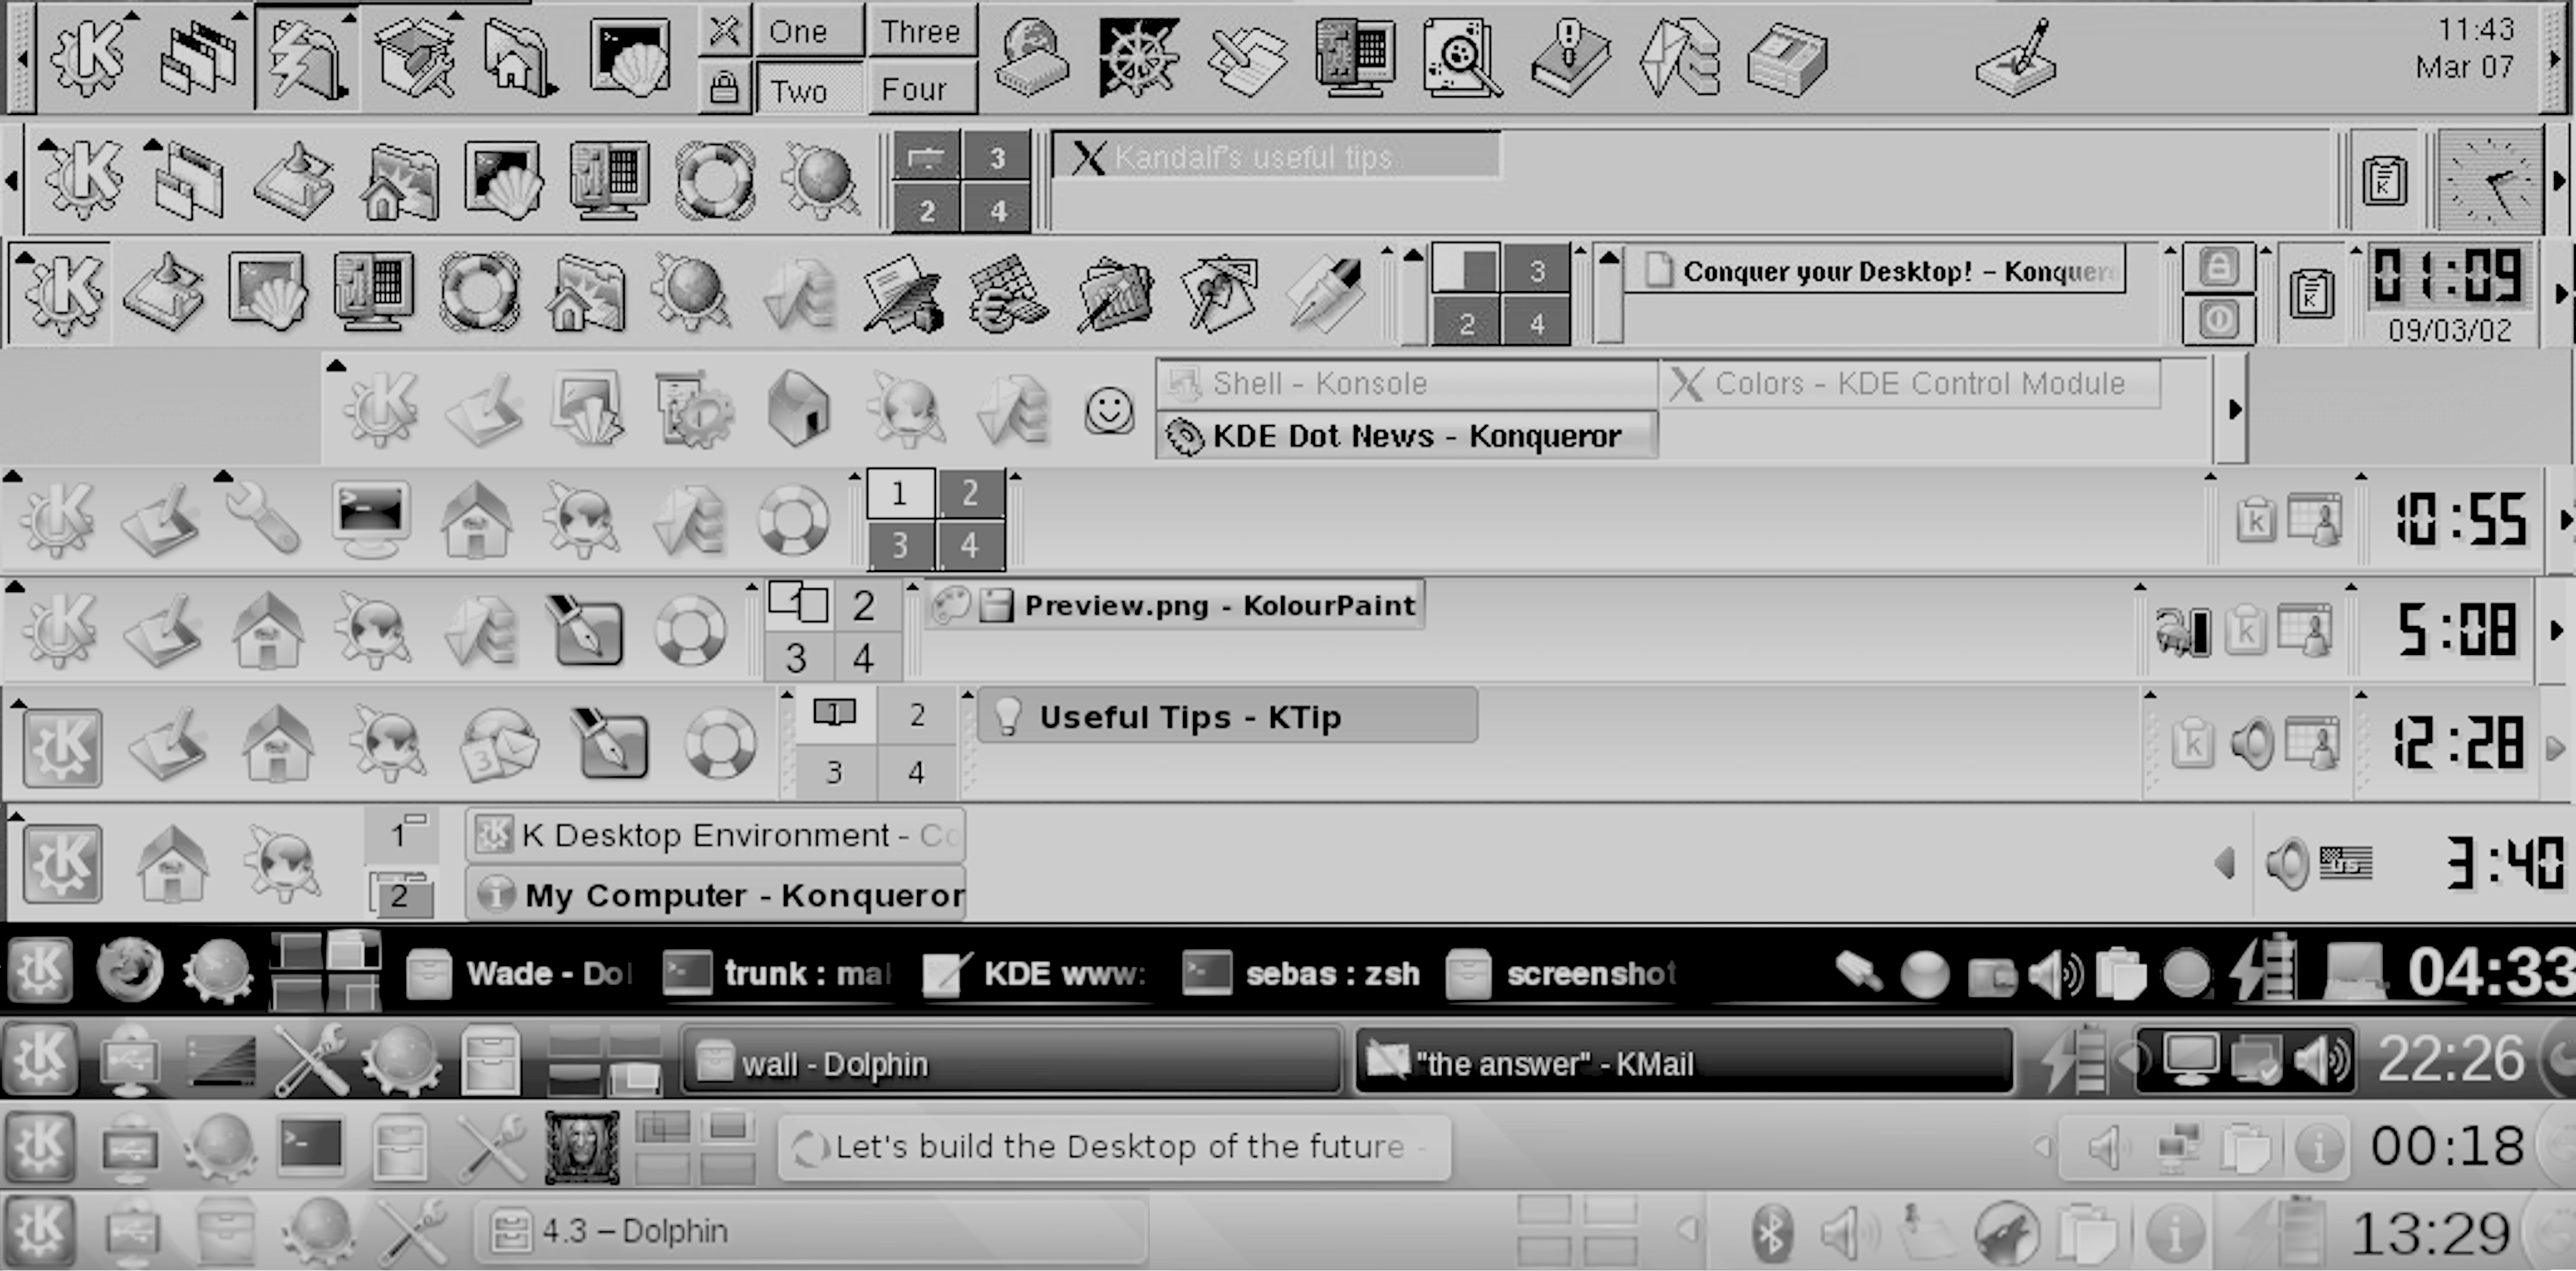
\includegraphics[scale=0.28]{images/images_thulin/kde_barre_outils.png} 
\caption{Évolution des barres d'outils de l'environnement KDE (la version 4.0 est en noir comme dans MS Vista). Les 8 premières versions utilisent un fond grisé, la suivante est noire, les trois dernières utilisent un fond bleuté sobre.}
\end{figure}


\section*{4.~~~OpenOffice et l'apprentissage de la grammaire visuelle}
\phantomsection
\addcontentsline{toc}{section}{4. OpenOffice et l'apprentissage de la grammaire visuelle}

Dans les deux exemples précédents, nous avons montré que la culture
numérique (niveau théorique) ainsi que les fonctionnalités techniques
(niveau applicatif) sont des contraintes qui structurent les deux
premières libertés du logiciel libre, qui sont celles de l'étudier et
de l'améliorer. Nous abordons maintenant la troisième liberté, qui est
d'utiliser un logiciel libre, en nous concentrant cette fois sur le
niveau interprétatif. Ce niveau est le niveau le plus connu du lecteur,
puisqu'il s'agit de la manière dont l'utilisateur comprend ce qu'il
voit à l'écran sans avoir accès au code qui génère les formes visuelles
perceptibles. Aussi, nous préciserons en quoi la «~grammaire visuelle~»
sous-tend notre perception et donc nos usages. 

La troisième liberté qui est d'utiliser librement un logiciel libre nous
semble doublement limitée : par le temps d'apprentissage de
l'utilisateur, et par le coût de sa formation (coût de temps, d'énergie
et d'argent). En effet, pour comprendre une interface, l'utilisateur
doit savoir interpréter le rôle des formes visibles, savoir celles qui
sont manipulables, anticiper les réactions, connaître un ensemble de
conventions propres au genre de l'application ou au logiciel lui-même,
etc. C'est cette activité sémiotique, de perception et d'interprétation
simultanée des formes visibles, qui nous permet d'interagir avec un
écran. Les développeurs d'interfaces graphiques savent de façon
consciente ou non qu'il est possible de réutiliser un ensemble d'objets
visuels de façon à profiter de l'expérience de l'utilisateur : c'est le
cas des fenêtres, des icônes ou des menus. De même qu'un adepte de la
console, ou interface en ligne de commande (\textit{Command Line
Interface}) doit connaître une syntaxe particulière pour pouvoir
l'utiliser, il existe un langage informatique visuel, assujetti à une
«~grammaire visuelle~» qui doit être connue de l'usager pour utiliser
une interface graphique (\textit{Graphic User Interface}).

Cependant, comme le remarquent Kress et Leeuwen\footnote{\cite{kressreading2006}.}, toute grammaire
visuelle n'est pas structurée de manière fixe : elle évolue avec le
temps, en particulier en fonction des relations sociales qui
définissent la manière dont nous interprétons telle ou telle forme.
Appliquons cet outil\footnote{Pour décrire de
telles grammaires, ces auteurs étendent le champ de la linguistique
fonctionnelle de Halliday (1994) à tous les systèmes de communication
sémiotique. Ils distinguent trois métafonctions dans une grammaire
visuelle que nous réutilisons dans la table (infra) : \begin{itemize}
\item la métafonction idéationnelle, qui relie deux objets de façon
relationnelle ou hiérarchique afin de représenter des idées au sujet du
monde naturel ;
\item la métafonction interpersonnelle, qui manifeste des relations
sociales entre le producteur, l'observateur et l'objet représenté ;
\item et la métafonction textuelle, qui indique des relations internes à
une forme sémiotique, lesquels forment des «~textes~» : un complexe de
signes qui adhèrent entre eux et au contexte, et pour lequel l'ordre ou
l'arrangement est tout à fait signifiant.
\end{itemize}
} à l'évolution d'OpenOffice versions 3.2 et 3.3 ainsi qu'au projet
intermédiaire Renaissance. L'analyse des métafonctions permet de
caractériser les interfaces et de les différencier (Cf. tabelau infra). Nous reprenons maintenant cette analyse en
revenant sur l'histoire de ces versions. 

Comme pour le navigateur Mozilla, son histoire est marquée par le départ
des développeurs pour travailler à des projets similaires tout en
récupérant les sources, de tels \textit{forks} étant un phénomène
fréquent dans le monde du libre. Sun Microsystems a racheté la suite
propriétaire StarOffice en 1999 et a ouvert le code l'année suivante,
donnant lieu à la sortie de OpenOffice 1 en 2002. Oracle Corporation a
ensuite racheté Sun en 2010 mais s'est retirée du projet l'année
suivante tandis que la communauté crée Libreoffice. Sous la pression
d'IBM, le code d'OpenOffice est cédé à la fondation Apache. À l'heure
où est édité cet ouvrage, le code de la suite bureautique devrait être
déjà fusionné avec celui de la suite concurrente IBM Lotus Symphony\footnote{Développé principalement en Chine, IBM
Lotus Symphony n'était pas initialement un logiciel libre, mais un
\textit{freeware}, donc un logiciel gratuit dont le code n'était pas
ouvert.}. On trouve d'autres versions basées sur le code d'OpenOffice
comme Go-oo ou NéoOffice (adapté au Mac OS/X), OpenOffice4Kids (version
pour les enfants), etc. Or, hormis pour cette dernière, toutes ces
versions ont sensiblement une interface similaire, à la différence de
MS Office par exemple qui ne connaît aucun \textit{fork} mais a
profondément remanié son interface. 

Bien que le calendrier n'ait pas été tenu, il existait un projet de
renouvellement de l'interface important chez OpenOffice, le projet
Impress Prototype Renaissance de l'équipe UX
OpenOffice\footnote{\url{http://wiki.openoffice.org/wiki/Renaissance}.}. Une démonstration de la future interface du logiciel de présentation
pour Impress 3.3 a même été publiée en ligne en juillet 2009. La
comparaison des interfaces précédentes (3.2) et futures (3.3) au projet
Renaissance, comme sur la figure 2, permet de circonscrire le projet.
Il ressort de l'analyse des documents de travail et de la grammaire
visuelle des interfaces que le projet Renaissance a tenté d'initier une
rupture visuelle à partir d'un projet centré sur le service à rendre à
l'utilisateur, en privilégiant l'efficience \footnote{À la différence de l'efficacité,
l'efficience vise à réduire le nombre d'interactions et de formes
visuelles pour un même résultat.}. À la suite d'un comparatif réalisé
par l'équipe UX au sujet des concurrents propriétaires
d'OpenOffice, les designers semblent séduits par plusieurs points de
l'ergonomie de MS Office 2007, en reproduisant des formes similaires
comme au niveau de la barre d'outils. Pourquoi le projet Renaissance
n'est-il pas mis en œuvre ? D'une part les interfaces de MS Office sont
protégées par des brevets, rendant toute inspiration risquée sur le
plan juridique. D'autre part, les services autour d'OpenOffice peuvent
être vendus plus facilement dans la mesure où l'interface d'OpenOffice
est plus proche des perceptions des utilisateurs, habitués à MS Office
2000. Or, tandis que que MS Office 2007 a renouvelé son interface, la
possibilité pour OpenOffice de se rallier aux habitudes des
utilisateurs est un argument pour réduire les coûts de formation.
Enfin, on notera bien sûr les changements stratégiques des sociétés
impliquées qui jouent un rôle sur les décisions à prendre : le projet
Renaissance peut être arrêté pour des raisons de financement liés à une
restructuration des services ou à la révision des objectifs
stratégiques, etc. 

En éludant le projet Renaissance, le passage de la version 3.2 à la
version 3.3 introduit un changement d'objectif. Impress 3.2 proposait
un outil complet pour soutenir la communication orale pour tous, dans
une relation d'échange créatif entre utilisateurs et développeurs.
Apache OpenOffice 3.3 se veut un outil efficace voire puissant, tourné
notamment vers le partenariat et la communication d'entreprise
(présentation chiffrée, résultats et ventes, etc.). Le projet
Renaissance, malgré ses qualités ergonomiques, semble moins prendre en
compte l'historique des organisations impliquées sur le projet
OpenOffice en prétendant, comme son nom l'indique, procéder à un
renouveau radical\footnote{On pourrait ici
comparer le projet Renaissance au Phoenix, qui introduit bien une
renaissance dans l'histoire de Mozilla ; or les conditions sont en fin
de compte bien différentes, le projet OpenOffice n'ayant pas connu les
mêmes déboires et attentes que chez Mozilla, et n'ayant pas forcément
besoin de renaître.}. 

Ainsi, l'apprentissage de la grammaire visuelle par l'utilisateur dépend
de conventions sémiotiques, mais aussi de l'histoire technique : du
développement et de l'histoire des organisations soumises à des
impératifs économiques. La liberté d'utiliser un logiciel libre est
donc contrainte par le dispositif socio-économique dans lequel est
inséré le développeur. À leur tour, les usagers interprètent
différemment les interfaces en fonction de leur propre contexte
socio-économique, d'apprentissage, culturel, de loisir, etc. Un projet
ergonomique libre reste bien sûr possible, mais il doit fortement tenir
compte de l'histoire économique et sociale de la communauté des
développeurs qui oriente les usages.

\begin{table}
\begin{scriptsize}
\begin{tabularx}{10cm}{|p{2cm}|p{2cm}|p{2.5cm}|X|}
\hline 
~ & \textbf{Modèles idéationnels}  & \textbf{Relations interpersonnelles}  & \textbf{Agencement textuel} \\
\hline 
OpenOffice Impress 3.2  & Créativité : dire, commenter  & Échange  & Potentiel \\
\hline 
Prototype Renaissance  & Table rase et conviviale  & Service  & Efficience \\
\hline 
Apache OpenOffice 3.3  & Modèle économique, représentation mathématique  & Partenariat et entreprenariat  & Puissance \\
\hline 
\end{tabularx} 
\end{scriptsize}
\caption{Analyse métafonctionnelle de l'évolution d'OpenOffice}
\end{table}



\begin{figure}
\centering
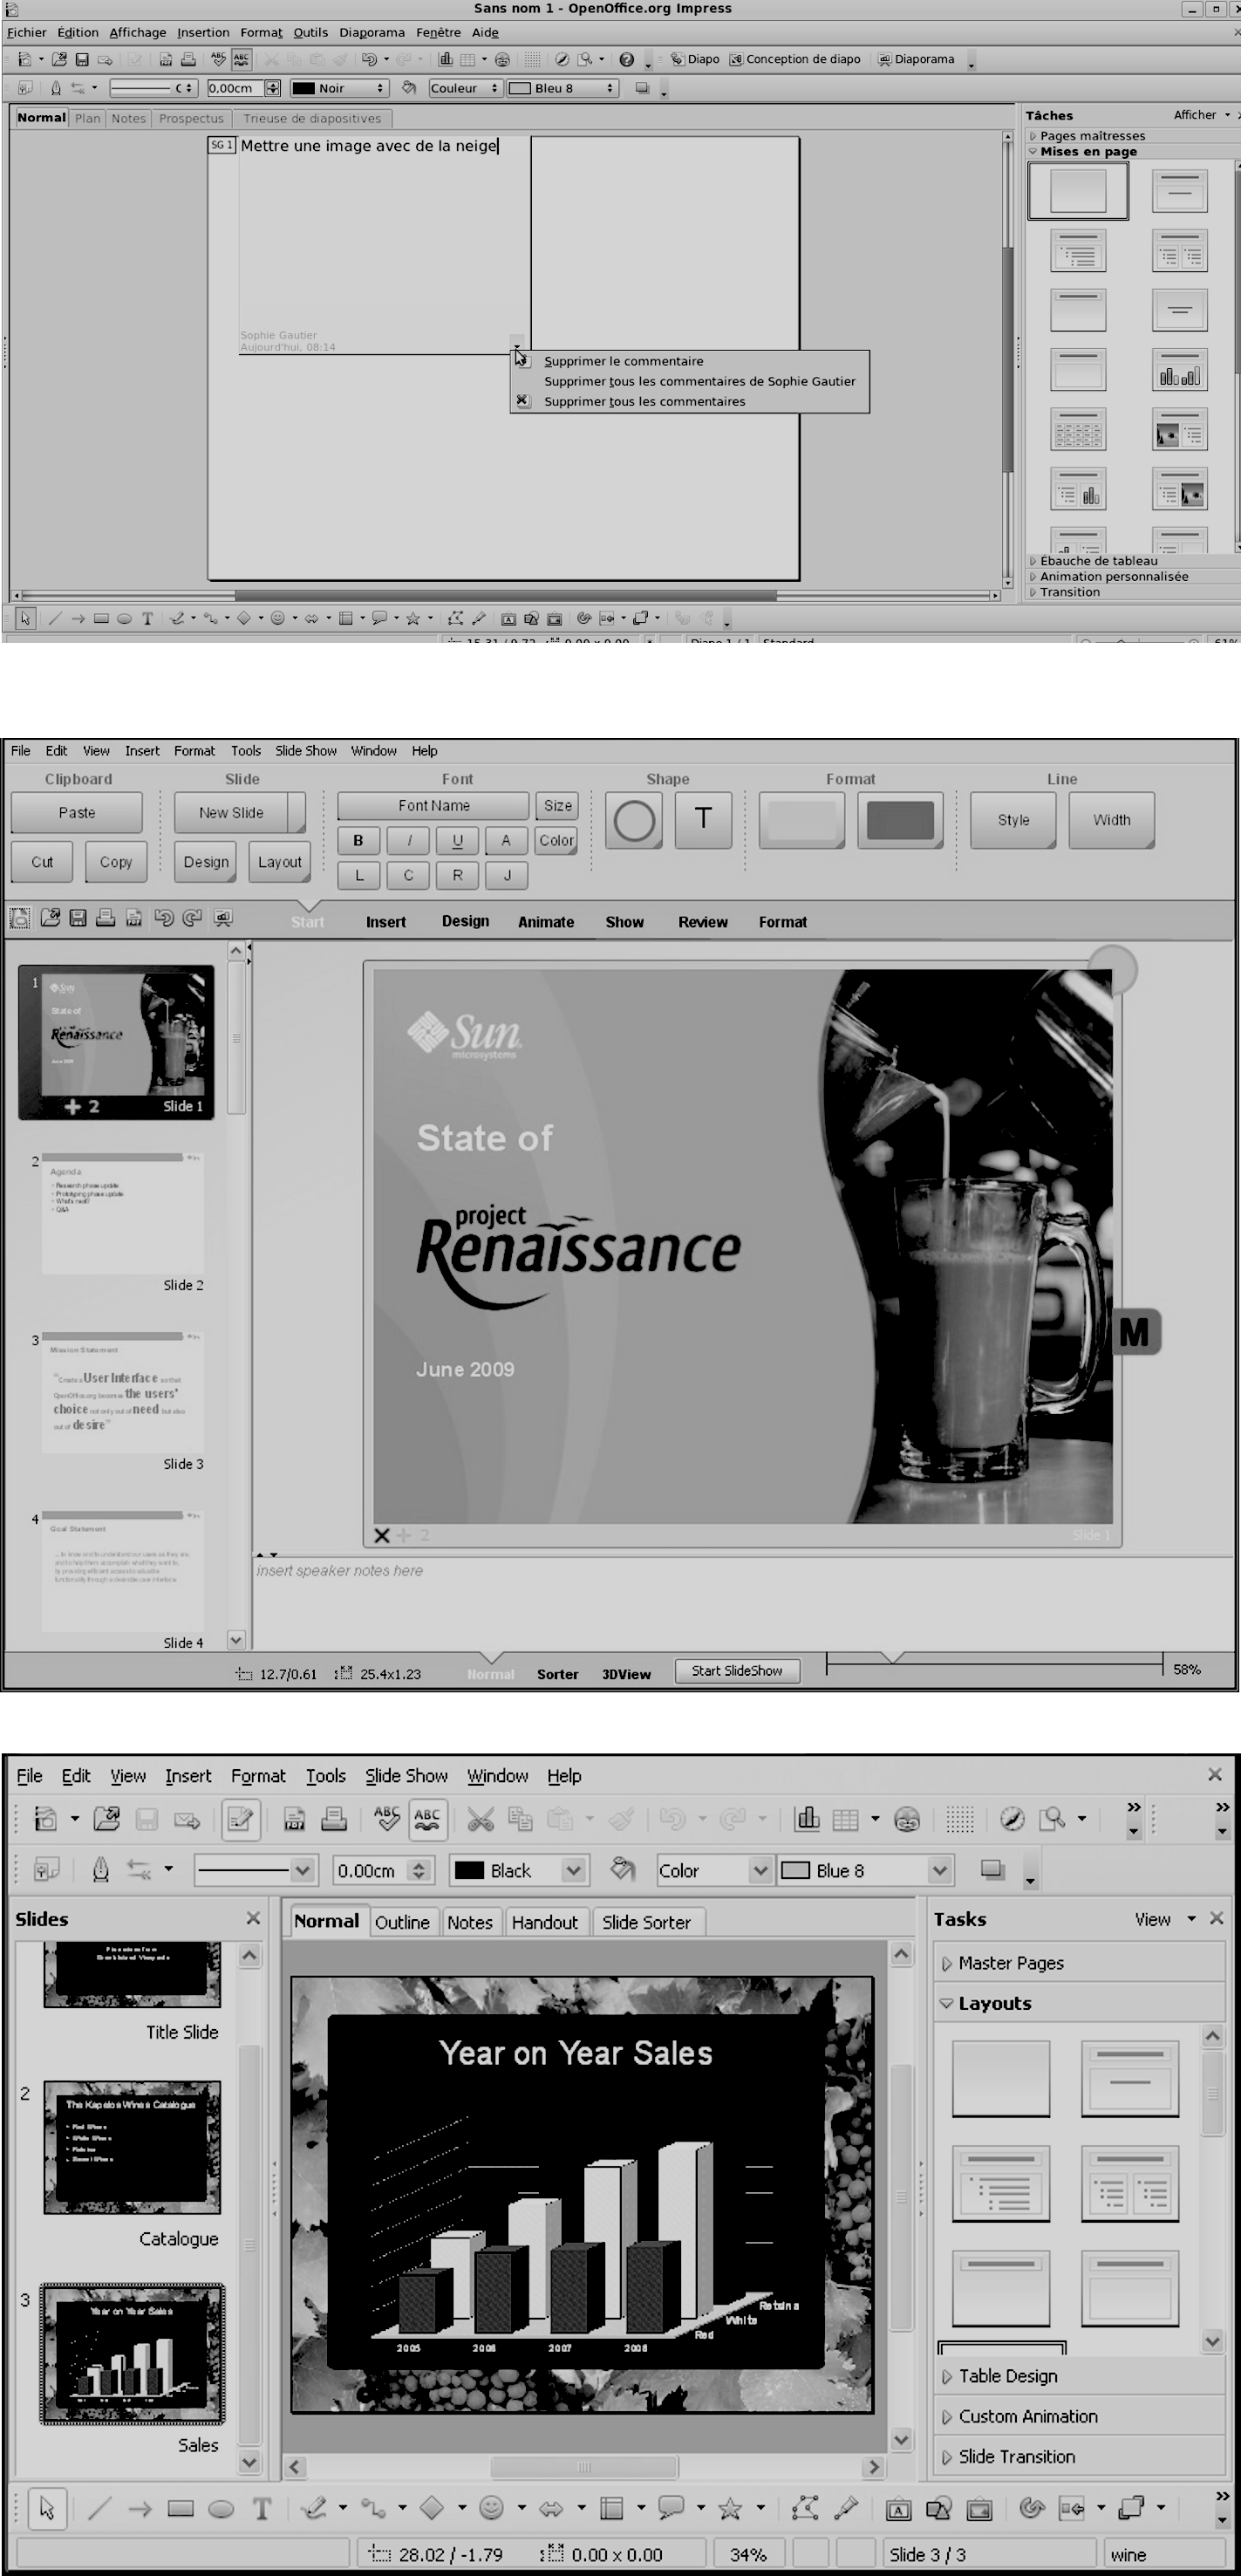
\includegraphics[scale=0.6]{images/images_thulin/Impress_comparatif.png}
\caption{Interfaces d'OpenOffice Impress 3.2, le projet Renaissance (non abouti) et Apache OpenOffice Impress 3.3.}
\end{figure}

\section*{5.~~~Comment Ubuntu ordonne-t-il le «~fatras sémiotique~» de ses utilisateurs}
\phantomsection
\addcontentsline{toc}{section}{5. Comment Ubuntu ordonne-t-il le «~fatras sémiotique~» de ses utilisateurs}


Après avoir étudié les trois premières libertés du logiciel libre, nous
abordons maintenant la dernière, la redistribution. Nous tentons ici de
saisir ce qui contraint, et donc structure, la redistribution. Nous
nous plaçons au «~niveau politique~» du numérique en étudiant ce en
quoi les normes sociales contraignent les formes visuelles. Nous
prenons comme cas d'analyse le bureau d'Ubuntu en raison de son
ambition démocratique clairement affirmée. 

Despres-Lonnet\footnote{\cite{despres-lonnetecrits2004}.} qualifie les «~écrits d'écran~» \footnote{L'écrit d'écran, notion initialement proposée par E. Souchier et Y. Jeanneret, définit la sémiotique de l'organisation des signes sur l'écran. \cite{souchierlenonciation2005}.} de «~fatras
sémiotique~» dans le cas des icônes de bureaux informatiques : les
lecteurs, ne parvenant pas à interpréter spontanément les «~signes
passeurs~»\footnote{La notion de signe passeur
pourrait remplacer celle de lien hypertexte dans la mesure où elle
montre aussi la fonction instrumentale du lien, mais montre davantage
le fait que la forme visuelle, le nœud, suppose que le lecteur
interprète la cible du lien à partir de ce qui est donné à voir.} que
sont parmi d'autres les icônes de bureau, sont conduits à mettre en
œuvre des stratégies mnémotechniques : ils retiennent l'usage lié à tel
symbole plutôt qu'ils ne décodent le symbole à chaque fois qu'ils le
voient\footnote{Une disquette continue de
signifier «~enregistrer~», bien que la disquette n'ai jamais été
manipulée par les jeunes générations.}. Si ce bazar peut désorienter,
il est par défaut extrêmement ordonné par un ensemble de règles et de
normes qui trouvent leur inspiration dans un projet de diffusion
général. Face à la multiplicité des systèmes d'exploitation qui
permettent de faire des tâches similaires, le choix de l'utilisateur
peut inclure des critères non techniques voire politiques. Dès lors,
comment des normes sociales ordonnent-elles le fatras sémiotique de nos
bureaux ? Compte tenu de la place dont nous disposons, nous ne
proposerons pas ici une étude de chacun des signes passeurs que sont
une icône ou une zone cliquable. Nous nous concentrerons sur les
changements visuels globaux des versions du bureau par défaut d'Ubuntu
comme dispositif symbolique articulant des formes, des sons, des
couleurs, des interactions, etc. Nous abordons ici le dispositif Ubuntu
(un lexique, des interactions, des formes visuelles, des couleurs, des
normes, des règles, des valeurs...) comme «~signe passeur global~» : à
côté de la fonction instrumentale de ce qui se donne à voir ou à lire,
il existe une fonction sémiotique qui suscite l'interprétation du
lecteur pour anticiper ce vers quoi l'amène une nouvelle version. Nous
nous situons donc sur le plan symbolique et social. 

La liberté de redistribuer des logiciels libres inscrit délibérément le
projet technique du libre dans le cadre d'un projet tourné vers la
société. À ce titre, le projet Ubuntu ambitionne de distribuer un
système d'exploitation à grande échelle. Avec cette ambition, Ubuntu
est capable de transformer ses valeurs en normes, de définir ce qui est
normal dans un projet libre. Lorsque le projet Ubuntu démarre en 2004 à
partir d'un \textit{fork} de la distribution de Linux Debian, il a pour
objectif de créer un système d'exploitation accessible au plus grand
nombre, ce qui aurait pour conséquence de «~démocratiser Linux~» ou de
produire une «~distribution
générique~»\footnote{Pour une discussion sur les conséquences de cette ambition sur les autres distributions, voir le texte d'Adrian Kingsley-Hughes - 02 avril 2008 - ZDNet.com, traduit en français sur le framablog \url{http://www.framablog.org/index.php/post/2008/04/06/distribution-ubuntu-substitution-linux}.}. Le projet Ubuntu propose alors par défaut l'environnement Gnome
comme bureau. Il est porté par le jeune entrepreneur sud africain
milliardaire Mark Shuttleworth via la société Canonical, à l'aide d'un
apport initial de 10 millions de dollars dans la fondation Ubuntu. En
référence à ses origines, l'entrepreneur a choisi un nom africain :
Ubuntu signifie en bantou «~humanité aux autres~», avec l'idée de
partage et de solidarité («~Je suis ce que je suis grâce à ce que nous
sommes tous~»). Le projet économique qui accompagne Ubuntu rejoint sa
«~philosophie~», qui se réfère à la promotion du logiciel libre et à
l'\textit{open source}, mais aussi au multilinguisme, à la gratuité, à la
non-discrimination des personnes. Des expressions comme «~tout
utilisateur devrait~» ou l'idée de «~reconnaissance mondiale~» montre
que l'ambition d'Ubuntu est de type
universaliste\footnote{À la différence du globe
présent dans certains logos de Mozilla pouvant évoquer une «~planète
martienne~», le logo d'Ubuntu ne représente pas la terre mais l'humain
solidaire ; certaines photographies représentent des personnes pouvant
être issues de continents différents. Il n'y a donc pas d'univers
Ubuntu mais bien une ambition universaliste liée à un projet économique
à l'échelle mondiale.}. Cette ambition vise, à partir d'une vision
technique, à promouvoir une certaine forme de société. Le passage des
valeurs aux normes apparaît avec le projet politique d'Ubuntu,
lorsqu'il définit un «~code de conduite~» ainsi qu'une «~politique de
gouvernance~» pour sa communauté. Dans ces documents, Ubuntu cadre le
vivre ensemble à partir de valeurs comme la prévenance, le respect, la
collaboration, la consultation, la responsabilité, etc. Ces valeurs,
érigées en normes, fournissent donc un cadre politique à l'idée de
libre distribution, lequel permet de dire quel comportement est jugé
normal, et quel comportement est soumis à sanction. L'idée de
«~communauté~» montre bien que si une personne ne se conforme pas aux
règles avancées, elle puisse être sanctionnée \textit{a minima} par la
non-appartenance à cette communauté. Enfin, ces normes dépassent la
sphère de la communauté puisque la «~méritocracie ouverte~» prônée par
Ubuntu constitue une invitation adressée à «~tout le monde de n'importe
quelle
entreprise.~»\footnote{\url{http://www.ubuntu.com/project/about-ubuntu/conduct}.}

Ces choix éthiques ou politiques s'inscrivent aussi dans les interfaces
de la distribution, et notamment le bureau. Par exemple, les choix de
palettes de couleurs connaît une évolution certaine. La première
version d'Ubuntu assume nettement sa différence d'avec les autres
distributions de Linux, avec un fond de bureau couleur châtaigne, qui
connote la terre ou le bois, une certaine authenticité. Les versions
suivantes dérivent vers l'orange, en particulier au niveau des icônes,
ce qui renvoie à plus de modernité et de convivialité. Le violet des
dernières versions, au moment de l'arrivée de la nouvelle interface
Unity (Ubuntu 10.04), est liée dans la culture occidentale à l'autorité
des évêques et au rite d'initiation : ce choix peut s'expliquer par un
compromis entre les couleurs initiales et une volonté de devenir une
référence sur un marché des systèmes d'exploitation concurrentiel.
L'inversion vidéo des barres de menu, comme lors de la sortie de
Windows Vista, se conforme avec la diffusion en masse d'ordinateurs
noirs, ce qui à l'origine a surtout pour but d'éviter la traces de
doigts. Les bandes noires peuvent aussi renvoyer au cinéma, à son cadre
intimiste, tout en nous donnant l'impression d'assister à une histoire
extraordinaire, en connotant force et confidentialité. Dans une
certaine mesure, l'évolution des chartes graphiques effectue un
contrepoint par rapport à d'autres dimensions sémiotiques de la
distribution. Par exemple, les noms des différentes versions d'Ubuntu
correspondent à des animaux dans la filiation du bestiaire exotique du
libre. Ces animaux sont un peu des «~signes passeurs~» puisqu'ils
annoncent une nouvelle version, tout en nous invitant à les interpréter
à partir des qualités que nous prêterions à ces animaux. Nous proposons
dans le tableau suivant une interprétation de ces signes : noms,
couleurs, formes iconiques, menus, etc. Les adjectifs sont
particulièrement évocateurs. Par là, les premières versions renvoient à
l'idée de recherche d'un positionnement, à de l'auto-dérision
(verruqueux, vénérable, jovial, pimpant, nerveuse), puis à la recherche
de reconnaissance (téméraire, fougueux, robuste, intrépide, enjoué).
Les versions suivantes renvoient davantage aux qualités marketing d'un
produit à distribuer (karmique, lucide, non-conformiste, chic,
onirique, précis). 

Ainsi, la diversité et la richesse du libre ne consiste pas à faire une
interprétation directe des valeurs du libre. Sur le plan des couleurs,
notons qu'à son origine, le marron était censé évoquer l'humanité ou la
chaleur\footnote{Cf. l'explication que donne M. Shuttleworth sur le wiki d'Ubuntu
\url{https://wiki.ubuntu.com/MarkShuttleworth\#Why_is_the_default_desktop_in_Ubuntu_BROWN.3F}.}. Le marron chaleureux de la terre contraste avec le bleu froid du
ciel de certains de ses concurrents, tandis que le son du djembé au
démarrage nous renvoie à des clichés de l'imaginaire africain
occidental. L'histoire du bureau ne montre qu'un ensemble de dérivés
par rapport à cette première idée. Les valeurs du libre s'expriment
donc à travers les interfaces graphiques tout au long d'une histoire
collective propre au projet. Pour les développeurs d'Ubuntu, «~notre
philosophie est reflétée dans les programmes que nous produisons et
incluons dans notre distribution.~»\footnote{\url{http://www.ubuntu.com/project/about-ubuntu/our-philosophy}.}

\begin{landscape}
\begin{table}
\centering
\begin{scriptsize}
\begin{tabularx}{15cm}{|p{1.5cm}|p{1cm}|p{1.5cm}|X|p{2cm}|p{2cm}|p{1.5cm}|}
\hline
 \textbf{Date} &  \textbf{Version}  & \textbf{Nom de code}  & \textbf{Changements visuels}  &  \textbf{Effet}  &  \textbf{Qualificatif}  & \textbf{Mascotte} \\
\hline
 2004-10-20  &  4.10  &  Warty Warthog  & Couleurs marrons dominantes  &  Authenticité  &  verruqueux  &  phacochère \\
\hline
 2005-04-08  &  5.04  &  Hoary Hedgehog  & Bureau plus lumineux  &  Performance  &  vénérable  & hérisson \\
\hline
 2005-10-13  &  5.10  &  Breezy Badger  & Le logo d'Ubuntu devient orange et remplace celui de Gnome  &  Affirmation  & jovial  & blaireau \\
\hline
 2006-06-01  &  6.06 LTS  &  Dapper Drake  & Thème orangé  &  Modernité  &  pimpant  &  canard \\
\hline
 2006-10-26  &  6.10  &  Edgy Eft  & Réduction du nombre d'écrans de bureau, l'icône de Firefox remplace l'icône standard ; apparition de l'icône d'aide  &  Simplicité  &  nerveuse  & salamandre \\
\hline
 2007-04-19  &  7.04  &  Feisty Fawn  & L'icône du courrielleur se simplifie, arrivée de nouveaux applets  &  Perfection  &  téméraire  & faon \\
\hline
 2007-10-18  &  7.10  &  Gutsy Gibbon  & Applet comportant le nom de l'utilisateur  &  Personnalisation  &  fougueux  & gibbon \\
\hline
 2008-04-24  &  8.04 LTS  &  Hardy Heron  & Le nom est remplacé par l'icône d'un personnage en vert  &  Optimisme  &  robuste  & héron \\
 \hline
  2008-10-30  &  8.10  &  Intrepid Ibex  & L'icône verte est remplacé par un bouton de démarrage rouge avec le nom & Technicité  & intrépide  & bouquetin \\
\hline
\end{tabularx}
\end{scriptsize}
\caption{Histoire du bureau d'Ubuntu (1/3)}
\end{table}
\end{landscape}




\begin{landscape}
\begin{table}
\centering
\begin{scriptsize}
\begin{tabularx}{15cm}{|p{1.5cm}|p{1cm}|p{1.5cm}|X|p{2cm}|p{2cm}|p{1.5cm}|}
\hline
\textbf{Date} &  \textbf{Version}  & \textbf{Nom de code}  & \textbf{Changements visuels}  &  \textbf{Effet}  &  \textbf{Qualificatif}  & \textbf{Mascotte} \\
\hline
 2009-04-23  &  9.04  &  Jaunty Jackalope  & Pas de différence visuelle notable  & ~ & enjoué  & jackalope \\
\hline
 2009-10-29  &  9.10  &  Karmic Koala  & Retour à un thème plus sobre ; les icônes des applets passent en noir et blanc, apparition d'une icône de courrier  &  Sobriété  &  karmique  & koala \\
\hline
 2010-04-29  &  10.04 LTS  &  Lucid Lynx  & Les couleurs vidéos des barres d'outils s'inversent (texte gris sur fond noir), retour de plusieurs écrans du bureau ; disparition de l'icône d'aide  & Évasion  & lucide  & lynx \\
\hline

 2010-10-10  &  10.10  &  Maverick Meerkat  & Apparition d'un thème violet, usage du services sociaux sur le bureau (Gwibber)  &  Leader  & non-conformiste  & suricate \\
\hline
 2011-04-28  &  11.04  &  Natty Narwhal  & L'interface Unity remplace celle de Gnome  &  Ergonomie  &  chic  & narval \\
\hline
 2011-10-13  &  11.10  &  Oneiric Ocelot  & Révision du menu latéral, le logo d'Ubuntu s'agrandit en devenant une icône de ce menu aux côtés de LibreOffice  &
 Affirmation  &  onirique  & ocelot \\
\hline
\end{tabularx}
\end{scriptsize}
\caption{Histoire du bureau d'Ubuntu (2/3)}
\end{table}
\end{landscape}


\begin{landscape}
\begin{table}
\centering
\begin{scriptsize}
\begin{tabularx}{15cm}{|p{1.5cm}|p{1cm}|p{1.5cm}|X|p{2cm}|p{2cm}|p{1.5cm}|}
\hline
\textbf{Date} &  \textbf{Version}  & \textbf{Nom de code}  & \textbf{Changements visuels}  &  \textbf{Effet}  &  \textbf{Qualificatif}  & \textbf{Mascotte} \\
\hline
 2012-04-26  &  12.04 LTS  &  Precise Pangolin  & Retour du nom d'utilisateur en haut à gauche, réduction du nombre d'applications dans le menu latéral  &
 Précision  &  précis  & pangolin \\
\hline
 2010-10-10  &  10.10  &  Maverick Meerkat  & Apparition d'un thème violet, usage du services sociaux sur le bureau (Gwibber)  &  Leader  & non-conformiste  & suricate \\
\hline
 2011-04-28  &  11.04  &  Natty Narwhal  & L'interface Unity remplace celle de Gnome  &  Ergonomie  &  chic  & narval \\
\hline
 2011-10-13  &  11.10  &  Oneiric Ocelot  & Révision du menu latéral, le logo d'Ubuntu s'agrandit en devenant une icône de ce menu aux côtés de LibreOffice  &
 Affirmation  &  onirique  & ocelot \\
\hline
 2012-04-26  &  12.04 LTS  &  Precise Pangolin  & Retour du nom d'utilisateur en haut à gauche, réduction du nombre d'applications dans le menu latéral  &
 Précision  &  précis  & pangolin \\
\hline

\end{tabularx}
\end{scriptsize}
\caption{Histoire du bureau d'Ubuntu (3/3)}
\end{table}
\end{landscape}




\printbibliography[heading=subbibliography]
\end{refsection}
 
% -------------------------------------------------------------------------
%
%%%%%%%%%%%%%%%%%%%%%%%%%%%%%%%%%%%%%%%%%%%%%%%%%%%%%%%%%%%%%%%%%%%%%%%%%%%%
%
\part{Études de cas}
\phantomsection
%\addcontentsline{toc}{part}{Études de cas}
%
%%%%%%%%%%%%%%%%%%%%%%%%%%%%%%%%%%%%%%%%%%%%%%%%%%%%%%%%%%%%%%%%%%%%%%%%%%%%
%

%--------------------------------------------------------------------
\chapter*{\textit{Pure data}, logiciel libre de productions créatives}
\phantomsection               
\addcontentsline{toc}{chapter}{\textit{Pure data}, logiciel libre de productions créatives \\ \textit{Séverine Giordan}}
%--------------------------------------------------------------------

\fancyhead[LO]{\small \textit{Pure data}, logiciel libre de productions créatives}
\fancyhead[RE]{\small Séverine \textsc{Giordan}}
%%\setcounter{section}{0}
\begin{refsection}

\begin{flushright}
Séverine \textsc{Giordan}
\end{flushright}
\vspace{10 mm}


«~Pd~» acronyme de «~Pure Data~», encore dénommé «~générateur de codes
créatifs~» ou «~mécano cybernétiques~»\footnote{Voir Roland \textsc{Cahen}, \url{http://impala.utopia.free.fr/pd/patchs/PureData_Initiation_fr.pdf},
présentation Jérôme Abel.} est présenté aujourd'hui, et dans un sens
général, comme un logiciel à programmation graphique pour les créations
musicales, multimédias en temps réel. Toutefois, \textit{Pure Data} s'affranchit
largement de cette définition générique. \textit{Pure Data} est un logiciel
libre. Le programme informatique du logiciel est consultable,
manipulable par tous. Cette caractéristique a étoffé ses fonctions,
redirigé ses pistes de recherche et rendu possibles de nouvelles
méthodes, de nouvelles problématiques, de nouvelles applications,
provenant des pratiques des utilisateurs.

Nous chercherons ici à cerner le coefficient utopique de ce logiciel
libre : initie-t-il des actions collectives, des mutualisations, des
contributions, des relations équilibrées entre concepteurs et
utilisateurs constituées à partir des usages ?

Où se situe \textit{Pure Data} dans le paysage contrasté des logiciels libres ?
Dans un premier temps, l'histoire du logiciel
permettra de comprendre son évolution. Puis nous verrons comment des
communautés autour du logiciel \textit{Pure Data} ont émergé. Comment se
forment-elles ? Quelles sont leurs dynamiques et leur état
d'esprit ? Enfin, les atouts de ce logiciel libre
seront révélés. Ils éclairent les processus d'émergence et font
entrevoir de nouvelles formes de coopérations personnelles ou
institutionnelles, voire de solidarités. La diffusion et
l'apprentissage de ce logiciel montrent comment de nouvelles économies,
des industries créatives même, peuvent apparaître.

\section*{1.~~~\textit{Pure Data}, un logiciel de programmation visuelle}
\phantomsection
\addcontentsline{toc}{section}{1. \textit{Pure Data}, un logiciel de programmation visuelle}

\textit{Pure Data} est à l'origine un logiciel de programmation graphique sur un
mode visuel ou auditif\footnote{\cite[p.~21]{Pachet2004}.}. Un «~patch~», morceau de code qui
conduit à la création d'un comportement en temps réel est créé par un
ensemble de boîtes\footnote{Des «~objets~», qui sont l'instance de
classe, c'est-à-dire l'instance de données et de manipulateurs de
données.} (fonctions) liées les unes aux autres. Ce langage de
programmation non linéaire rappelle des studios électroniques ou encore
des synthétiseurs modulaires: «~le résultat d'un calcul que vous avez
effectué quelque part sera dirigé au moyen d'une connexion vers un
module quelconque qui lui même sera redirigé, vers un autre module
etc...~»\footnote{Voir Archives \textsc{Ircam}, \textit{Manuel Max}, p.~1.}. De la sorte,
les signaux électriques produits se déplacent de modules en modules. 

Le graphisme du logiciel est une évocation des programmes modulaires à
l'origine des premiers synthétiseurs modulaires analogiques, inventé
par Max Mathews, premier directeur scientifique de l'IRCAM à la fin des
années 1970. Il s'agit d'un programme orienté objet
contre la programmation procédurale plus usuelle. 

Le «~programme orienté objet~» fonctionne sur un système modulaire. Ce
parti-pris favorise l'autonomie de la pluralité des possibilités du
logiciel. L'interface graphique de programmation a été
pensée par rapport aux utilisateurs qui ne se sont pas forcément
initiés à la programmation informatique, et ne les oblige donc pas à
coder. Ce type de programmation rend abordable, accessible, ludique et
appropriable un domaine de compétences scientifiques et technologiques
qui peut sembler hermétique, lorsqu'il est observé du point de vue de
l'apprentissage du langage informatique.

\section*{2.~~~Dialogue entre scientifiques et artistes}
\phantomsection
\addcontentsline{toc}{section}{2. Dialogue entre scientifiques et artistes}

\textit{Pure Data} est issu de différents projets. Ils se nomment respectivement
\textit{4X}, \textit{Pattern Matching}, \textit{Patcher}, \textit{Max}, \textit{Max/MSP} ou \textit{JMax}… Lors de sa mise au
point, il a «~voyagé~» dans les plus grandes institutions de recherche
du monde. L'IRCAM\footnote{Institut de Recherche et de Coordination
Acoustique / Musique.}, Institut de Recherche et de création musicales
associé au Centre Pompidou, établissement public à caractère culturel,
fut un point de départ. 

La politique de l'IRCAM et certains de ses projets permettent de
comprendre l'évolution de ce logiciel. Cette institution a toujours eu
un axe majeur spécifique qui est le dialogue entre la recherche
scientifique et la création. Ce dialogue a pour vocation de conduire à
de nouvelles formes expressives, créatives, nourrissant tout autant les
inventions des musiciens, que celles des scientifiques. L'IRCAM est
très attentif aux liens possibles entre la culture musicale, son
histoire, ses formes et les processus scientifiques et technologiques.
Les résultats de ces recherches sont appropriées par des processus
artistiques et conduisent alors à l'émergence de questionnements
nouveaux. Pierre Boulez\footnote{Compositeur, chef d'orchestre.
Directeur de l'IRCAM de 1977 à 1992.}, directeur de l'IRCAM, reproche au
GRM\footnote{Pierre Boulez emploie l'expression «~bricolage
empirique~» pour qualifier les expérimentations du GRM. Voir \cite[p.~297]{Grynszpan2004}.
Le GRM, créé en 1958, est le centre de
recherche musical dans le domaine du son et de l'électroacoustique au
service de la recherche de radio-télévision française ORTF, INA.}
(Groupe de recherche musicale) d'instrumentaliser les
processus artistiques à des fins scientifiques et technologiques.
L'élaboration d'outils, de méthodes, de synthèses sonores, de création
d'instruments de musiques, d'analyse, de traitements, de
transformations du son en temps réel, des dispositifs d'acoustique
sonore dans l'espace furent et restent les fruits de cette institution.

L'IRCAM, afin de répondre à sa politique artistique et
culturelle, a choisi dès sa création de prolonger les recherches de Luciano Berio du
Studio de phonologie musicale de la RAI à Milan en enrichissant la 4A
qui est un empilage d'une soixantaine de calculateurs (1976), émettant
de multiples sons de manière autonome, en \textit{4X} (1978). Cette machine
donne la possibilité de varier les paramètres du son en temps réel
grâce à la vélocité de calculs de centaines d'oscillateurs. La \textit{4X} sous
la direction technique de Peppino di Giugno, permis à l'époque de jouer
par exemple la pièce sonore «~Repons~»\footnote{Œuvre de Pierre Boulez
(1981-1982-1984) avec comme sujet le dialogue entre jeu individuel et
jeu collectif avec comme formation 6 instruments solistes, un ensemble
instrumental et un système électro-acoustique pour transformer et
spatialiser le son des solistes. Voir \url{http://brahms.ircam.fr/works/work/6997}.} de Pierre
Boulez. La vitesse de calcul joue un rôle majeur dans l'évolution et la
simulation du suivi en temps réel des comportements instrumentaux,
dans l'intégration des phénomènes d'interprétation à la composition musicale
 et électroacoustique, de l'analyse du signal\footnote{\textit{Stereolux},
(Journées du code créatif 29-30 mars 2012) -- Miller Puckette précise les
moments clés des avancées technologiques pour le temps réel au début de
son intervention.}.

Miller Puckette, résident de l'IRCAM, mathématicien du
MIT\footnote{Massachusetts Institute of Technology}, travaille en
1985 à un programme nommé \textit{Pattern Matching} qui assure le recouvrement
entre un instrument de musique et une interprétation
électronique\footnote{Archives IRCAM, \textit{Atelier de recherche Musicale},
14.11.1985.} et soutien la cohérence entre les deux jeux. L'application
reconnaît les timbres, les hauteurs et les harmonies du soliste, et la
«~machine~» peut suivre ce dernier dans l'évolution de son jeu. De 1986
à 1987, il développe \textit{Patcher}, qu'il définit en ces termes : «~contrôle
raffiné des synthétiseurs pour l'exécution Live~»\footnote{Archive
\textsc{Ircam}, \textit{Manuel Max}, p.~1}. \textit{Patcher}, environnement graphique de
programmation musicale en temps réel, est l'aboutissement du travail
commun du compositeur Philippe Manoury et du mathématicien-programmeur
Miller Puckette\footnote{«~Miller Puckette travaille principalement à
rendre le programme fiable et maniable~».\cite[p.~40]{Ircam1995}.}, avec lequel ils créent l'œuvre musicale
\textit{Jupiter}\footnote{Prix de la meilleure réalisation musicale de la
SACEM en 1988.}. Il s'agit d'une
pièce dont l'environnement informatique (\textit{4X}, 1986)
reconnaît la flûte. Jupiter est la première pièce du cycle \textit{Sonus Ex
Machina}\footnote{\textit{Sonus ex machina}, réalisé à l'Ircam est composé de
\textit{Jupiter} 1987~(pour flûte), \textit{Pluton} 1988, 1989~(pour piano),~\textit{La Partition
du Ciel et de l'Enfer}, 1989~(pour orchestre) et \textit{Neptune} 1991(pour trois
percussionnistes), confrontées à la machine et à ses différents modes
de réaction.}. Philippe Manoury avait suivi un enseignement de la
composition musicale assistée\footnote{\textit{Zeitlauf} (1982) est la
première pièce de Philippe Manoury réalisée à l'IRCAM. Agencement de
chœurs mixtes, d'un ensemble instrumental, de synthétiseurs, de bandes
magnétiques.} par ordinateur et avait débuté cette forme de
composition avec l'IRCAM au début des années 1980. Dans \textit{Jupiter}, il
expérimente l'interaction instrument/machine en temps réel. À cette
fin, Philippe Manoury décrit trois types de démarche de composition
dans l'interaction instrument/machine : 

\begin{itemize}
\item La programmation est réalisée antérieurement. En live, la
transformation du rythme est envisageable, par contre les événements,
le découpage du temps sont fixés.
\item Le jeu peut être aussi lié à des calculs probabilistes.
\item Les signaux sonores provenant d'entrées Midi\footnote{Normes
d'échange de données musicales numérisées.} sont
interprétés par la machine.
\end{itemize}

La notion d'«~interprétation~» est alors questionnée à partir de ces
nouveaux possibles ; elle intègre les innovations scientifiques et
technologiques de Miller Puckette. Par exemple, dans la pièce
\textit{Pluton}\footnote{\url{http://brahms.ircam.fr/works/work/10493}.}
(1988-1989), \textit{Patcher} donne la possibilité d'étirer les sons. Philippe
Manoury expérimente alors notamment les prolongements des sons du
piano. La machine capte et collecte une séquence jouée par un pianiste: notes, rythmes, 
événements sonores, et l'ensemble de ces variables
hauteurs, durées, longueurs, dynamiques sont liés à des
règles\footnote{Par exemple pour cette pièce, l'artiste introduisait
les propriétés des chaînes de Markov, c'est-à-dire des développements
aléatoires qui ont pour conséquence des probabilités de successions
d'événements. Les traits stylistiques du soliste sont toutefois
maintenus. \cite[p.~111]{Langer2001}.}.

\textit{Patcher}, développé au départ sur la \textit{4X}, fut ensuite amélioré sur
l'ISPW\footnote{~IRCAM Signal Processing Workstation Stéréolux,
Conférence Miller Puckette.}, la Station d'informatique musicale, une
machine plus performante. \textit{Patcher} devient alors Max\footnote{Ce nom a
été donné en hommage de Max Mathews.} en 1990. Il n'est plus un
programme spécifiquement élaboré pour une seule pièce. Il se présente
comme «~universel~» et le
«~soft~»\footnote{L'expression Soft provient de
«~software,~», qui signifie logiciel en anglais.} se conforme à toutes
pièces musicales. Cependant, le passage entre les deux machines ne se
fait pas sans difficultés : toutes les pièces furent
recompilées\footnote{Passage d'un langage
informatique à un autre langage informatique.}. La puissance de calcul
des PC rend alors possible la diffusion du logiciel hors de l'IRCAM et
donne l'opportunité de commercialiser le logiciel sous une licence
privée IRCAM, ce qui répond aux exigences économiques du centre de
recherche\footnote{\cite{Combes2007}.}.

C'est David Zicarelli, chercheur développant la
portabilité du logiciel sur PC à l'IRCAM, qui est alors responsable de
l'entreprise californienne Opcode Systems, elle-même chargée de cette
finalité commerciale. Parallèlement, de 1993 à 1994, il travaille à un
logiciel complémentaire à Max, le MSP, un logiciel de synthèse sonore
qui, d'une part, analyse et manipule le signal en temps réel sur PC et,
d'autre part, comporte une bibliothèque d'objets (de fonctions) à cet
effet. Miller Puckette et David Zicarelli travailleront ensemble pour
créer des passerelles entre les deux programmes.

En 1995 sont élaborés Max/FTS, Max NeXT/X par François Déchelle et
Maurizio De Cecco, deux nouvelles versions adaptées à la ISPW/NeXT/X,
l'ordinateur propre à l'IRCAM. En 1996, Miller Puckette, alors
professeur en musique au département Art et Informatique de
l'université de San Diego, participe à l'ICMC\footnote{International
Computer Music Conference (ICMC) Thessaloniki en Grèce, capitale
culturelle européenne en 1997.} avec comme objectif de reconstituer
Max. Ce projet est subventionné par le Conseil Intel Research pour le
Global Music Visuel\footnote{\url{http://www.visualmusic.org}.}. Une
version «~augmentée~» en résulte, elle concède une dimension graphique
au logiciel, ce qui en facilite largement son usage. Cette
correspondance du son à l'image était négligée par l'IRCAM. 

La partie graphique a été réalisée par le chercheur Mark Danks. Il
programma l'extension externe
GEM (Environnement graphique pour le multimédia) qui rend possible la
manipulation des flux, des fichiers vidéo, des images fixes, des
fichiers 3D en temps réel. Le GEM emploie la technologie de l'Open~GL,
très populaire pour les animations 3D ou pour les jeux vidéo.
L'Open~GL est une bibliothèque de calculs graphiques à
2 et 3 dimensions. Les musiciens/compositeurs Vibeke Sorensen et Rang
Steiner ont également participé à ce projet. La pièce musicale
\textit{Lemma}\footnote{Présentée le 27 septembre 1997 au club de Jazz Milos
à Thessaloniki.}, qui expérimente le rapport de l'interaction
instrument/machine dans un contexte multimédia, est le fruit de cette
collaboration.

Le logiciel \textit{Pure Data} est le produit de cette longue histoire. En 1998,
toujours à l'IRCAM, sous la responsabilité de François Déchelle et
Maurizio De Cecco, est réalisée une version libre de Max, JMax (le J de
JMax correspond à l'interface Java ajouté au logiciel), afin de
permettre la portabilité du logiciel sur les systèmes d'exploitation
libres. 

\section*{3.~~~Questions de licences}
\phantomsection
\addcontentsline{toc}{section}{3. Questions de licences}

Miller Puckette, qui a réécrit en entier le programme Max sous le nom de
\textit{Pure Data}, a conféré une licence BSD (Berkeley software distribution
license)\footnote{La licence BSD (Berkeley software distribution
license) est une licence libre utilisée pour la distribution de
logiciels. Elle permet de réutiliser tout ou une partie du logiciel
sans restriction, qu'il soit intégré dans un logiciel
libre ou propriétaire.} à son logiciel, contrairement à l'IRCAM qui
avait attribué une licence privée à Max. L'Open Source Initiative
(OSI)\footnote{L'OSI prône la qualité des
logiciels libres contre les logiciels propriétaires. Le logiciel libre
est défendu comme source de bénéfices économiques. «~Open source is a
development method for software that harnesses the power of distributed
peer review and transparency of process. The promise of open source is
better quality, higher reliability, more flexibility, lower cost, and
an end to predatory vendor lock-in.~». \textit{A contrario} la FSF considère le
logiciel libre à partir de l'utopie éthique et sociale qu'il
convoque.}, défendant les valeurs bénéfiques économiques du logiciel
libre, considère cette licence comme adéquate. La Free Software
Foundation (FSF), association qui promeut les vertus sociales et
éthiques du logiciel libre, a attesté les licences BSD version 2 et 3,
compatibles, à la licence publique générale (GPL). Cette dernière
garantit les libertés fondamentales suivantes : l'emploi du logiciel
pour tout usage, la possibilité de consulter le programme du logiciel
et de le manipuler selon ses nécessités, la diffusion de copies, le
partage de versions modifiées à la communauté. La version 1 de la
Licence BSD est rejetée par la FSF pour la clause 4, dite clause de
publicité. Cette clause occasionne la notification de
l'ensemble des auteurs et
organisations\footnote{\url{http://www.gnu.org/philosophy/bsd.fr.html}.}
qui ont collaboré à l'écriture des programmes, ce qui est considéré
comme une publicité par FSF. 

Plus exactement, \textit{Pure Data} est sous la licence BSD amplifiée. C'est une
licence BSD qui a retiré la clause 4 de sa rédaction. La redistribution
et l'usage sous forme de code source ou binaire,
modifié ou non, sont soumises aux condition suivantes :

\begin{enumerate}
\item Le copyright, la liste des conditions et
l'avertissement qui la suit doivent figurer dans le
code source redistribué.
\item La documentation et/ou les fichiers fournis avec une
redistribution sous forme binaire doivent faire apparaître le
copyright, la présente liste des conditions et
l'avertissement qui la suit.
\item Le nom de l'auteur ne saurait être utilisé dans
le but de promouvoir ou de légitimer un produit dérivé de ce programme
sans autorisation écrite préalable.
\end{enumerate}
Il s'agit d'une licence claire, concise, simple dans sa rédaction. Elle
ne limite aucun usage ; elle est permissive, contrairement à la licence
GNU GPL\footnote{Rédigée par Richard Stallman et Eben Moglen, dans un
premier temps.}. Elle est compatible avec des licences propriétaires.
Les clauses inscrivent le droit d'auteur, la liste des conditions,
l'avertissement dans la version modifiée et dans la documentation de la
version du code source et l'accord écrit des auteurs et de l'organisme
pour l'utilisation de leur auctorialité à des fins de cautionnement
scientifique et promotionnelle. 

La licence BSD n'est toutefois pas choisie par tous les contributeurs
développeurs de \textit{Pure Data}. Ce fut le cas par exemple de la librairie
GEM\footnote{Mark Danks, Chris Clepper, Cyrille Henry, IOhannes M
Zmoelnig, Guenter Geiger, Daniel Heckenberg, James Tittle,
Hans-Christoph Steiner et bien d'autres ont participé à sa création.}
(Graphics Environment for Multimedia), qui est sous licence GNU GPL.
Cette librairie a permis à \textit{Pure Data} d'être un environnement graphique
de programmation pour la création multimédia en temps réel donnant
libre cours à l'imagination des utilisateurs par rapport à la création
et les manipulations d'objet en 3D, de vidéos, d'images, de particules
grâce à l'open-GL\footnote{Conception d'applications
générant des images~2D et 3D.}. La licence GNU GPL applique le
\textit{copyleft} c'est-à-dire une protection des usagers et de la communauté du
libre à l'obligation aux versions du logiciel libre modifié de
conserver sa qualité de logiciel libre.

Le logiciel \textit{Pure Data} possède des librairies dans lesquelles
l'amateur trouve des «~objets~» qui lui donnent des
outils de création. L'«~objet~» \textit{[expr\textasciitilde]}, réalisé
par Aymeric Mansoux, Chun Lee et Olivier Laruelle, sous le nom du
collectif 0XA\footnote{\url{http://archive.org/details/GOSUB10-004}. «~\textit{[expr\textasciitilde]} is the first music release of 0xA, consists of retro sounding tracks made almost entirely with the \textit{[expr\textasciitilde]} object in \textit{Pure Data}. No  tweaking of number boxes and sliders, no clever generative algorithms, just switch the audio on and listen. The source code for this release (implemented in Pure-data) is free software distributable under the terms of the GNU General Public License (version 3 or greater). For repository, see: \url{http://gitorious.org/0xa}. Copyleft: This is a free work, you can copy, distribute, and modify it under the terms of the Free Art License. Released on 3rd April 2011.~»} qui permet la composition de sons 8
bits, ont édité cet objet sous la LAL, Licence Art Libre. Les
logiciels, les programmes informatiques sont ici compris comme des
œuvres de création, ce qui explique l'utilisation de
cette licence\footnote{«~Notre souci commun était que la Licence Art
Libre puisse répondre à trois conditions : qu'elle
soit conforme au droit français, qu'elle soit fidèle à
l'esprit du Copyleft de la General Public License et qu'elle
corresponde à nos intentions artistiques de partage de la création
nourrie de ce que nous savions d'un certain art
contemporain.~» \cite[p.~478]{Moreau2001}.} qui fut créée à partir d'une liste de
diffusion (Copyleft\_attitude@april.org) et lors des
rencontres Copyleft Attitude\footnote{Rencontres Copyleft Attitude
organisées par Antoine Moreau avec les artistes réunis autour de la
revue \textit{Allotopie}, François Deck, Antonio Gallego, Roberto Martinez et
Emmanuelle Gall.}. La Licence Art Libre stipule la possibilité de
diffuser, de copier, de transformer, d'exploiter gratuitement ou
commercialement une œuvre à la seule condition de rendre accessible
l'original, la matrice du produit dérivé. Les personnes utilisant
l'objet \textit{[expr\textasciitilde]} sont sous le joug de la LAL, attestée par la GNU
GPL. Or, malgré les différences des licences des extensions de Pure
Data, lorsque le logiciel est exécuté, seule la licence BSD apparaît.

Miller Puckette conserve le contrôle de l'expansion du noyau du
logiciel, c'est à dire la partie qui effectue les
programmes de base du logiciel. Il maîtrise également les lignes
directrices fortes : la fiabilité du logiciel, l'amélioration du temps
réel de celui-ci, l'enrichissement de la reconnaissance du signal de la
voix et la charte graphique\footnote{Cf. \textit{Les journées du code créatif}
(première édition) à Nantes, \textit{Stéréolux}. 29-30 mars 2012.}. Andrea
Mayr dans l'article «~Pd as Open Source Community~»\footnote{\cite{Mayr2004}.}
explique que la légitimité auctoriale du logiciel se trouve dans les
qualités de créations des programmes, de documentations et de
communication des développeurs, ce qui explique l'aura dominante de
Miller Puckette\footnote{Miller Puckette est depuis 1994 le directeur
associé du centre de recherche en arts et informatique de l'université
de San Diego.}. Pourtant, cette autorité non négociée a des limites :
des versions différentes DesireData ou Pd-l2Ork sont apparues,
prétendant une d'amélioration des programmes liés aux
programmes de base. De plus, certains programmeurs contribuent
désormais non plus à \textit{Pure Data} mais à d'autres
logiciels de programmation en temps réel comme SuperCollidor ou vvvv.

\section*{4.~~~La Communauté}
\phantomsection
\addcontentsline{toc}{section}{4. La Communauté}

\subsection*{4.1~~~Conventions et dispositifs de coopération}
\phantomsection
\addcontentsline{toc}{subsection}{4.1 Conventions et dispositifs de coopération}

Lors d'une résidence à l'IEM (Institut de musique acoustique et
électronique) de Graz en Autriche à la fin des années 1990 avec
certains étudiants et chercheurs de cette formation, Miller Puckette a
lancé les «~catalyseurs~» de la communauté. Ils ont produit tour à tour
une liste de diffusion, un wiki\footnote{\url{http://puredata.info}.}
dédié, un guide donnant la marche à suivre pour enrichir le
logiciel\footnote{Voir \url{http://pdstatic.iem.at/externals-HOWTO}, écrit par
Ioannes Zmölnig.} et un IRC (Internet Relay Chat). Ces outils
facilitent la coopération entre développeurs et simples amateurs de
\textit{Pure Data}. 

Ces dispositifs sont toujours opérants et, avec le temps, ils
rassemblent une communauté importante comportant de nombreuses
nationalités. Depuis lors, d'autres forums ont émergé. Ils ont pour
objectif principal de mettre en relation les utilisateurs de ce
logiciel à partir d'une communauté géographique ou de
langues\footnote{Voir \url{http://puredata.hurleur.com}, \url{http://gmane.org},
\url{http://codelab.fr/pure-data}, \url{http://www.puredata.it/forum},
\url{http://www.foroswebgratis.com/foro-pure\_data\_espana-77988.htm}, \url{http://createdigitalnoise.com/categories/pd-everywhere}.}.

L'IEM à l'origine de la liste de diffusion est également à l'origine de
la première \textit{Convention} tenue à Graz, en 2004. Ces conventions comportent des
conférences, des séminaires, des tables rondes, des ateliers, des
work in progress, des expositions, des performances et des concerts.
Chaque convention est spécifique ; elle est à l'image de l'équipe
d'accueil. La convention de 2007 à Montréal, \textit{L'œuvre ouverte}, s'est
donnée comme ambition, outre le dialogue entre utilisateurs,
développeurs et théoriciens, novices, et spécialistes, de développer
les points suivants :

\begin{itemize}
\item mobiliser la création artistique qui emploie les logiciels libres,
\item questionner la diffusion et la distribution libre,
\item cerner les aspects esthétiques et politiques de la culture du
logiciel libre,
\item montrer les pratiques ancrées dans une approche
multidisciplinaire,
\item mettre en lumière les structures locales de créations à partir du
libre,
\item intensifier les échanges entre domaines hétérogènes. 
\end{itemize}
Toutes les conventions (Graz, 2004; Montréal, 2007; Sao Paulo, 2009;
Weimar - Berlin, 2011) sont documentées par les écrits des
interventions, des photographies, récemment de vidéos. L'IEM a publié
les actes de de la première convention\footnote{\textit{Bang, Fribourg}, Frank \textsc{Zimmer} (éd.), 2004.}.

Par ailleurs, la communauté s'appuie sur des espaces et
des événements où les utilisateurs se forment et se rencontrent.

\subsection*{4.2~~~Les espaces de formations}
\phantomsection
\addcontentsline{toc}{subsection}{4.2 Les espaces de formations}

\paragraph{Labs et friches culturelles.}
De nouveaux lieux culturels (hacklabs, friches culturelles, espaces de
co-working, associations de logiciel libre) proposent des ateliers \textit{Pure
Data}. Ces espaces de création sont très singuliers du fait
qu'ils sont issus des acteurs qui les composent, à
l'espace géographique auquel ils appartiennent. Ces
espaces inventent leurs propres grammaires ancrées dans un contexte
socio-politique culturel contemporain. Ils ne copient ni les centres
d'animation municipaux, ni les centres d'art
contemporains ouverts dans «~les années 1980~». Il n'y a
pas véritablement une politique stricte qui les unissent. Les notions
d'émancipation, d'épanouissement personnel et collectif ne sont pas
suffisantes à les décrire. Certains se distinguent par la volonté
d'auto-gestion, d'autonomie,
d'autres la promotion de la création émergente, de la
sensibilisation des publics à la culture informatique et technique, aux
questionnements politiques, éthiques qui y sont liés. Espaces ouverts,
d'échanges, de débats, ils «~travaillent~» à reconstruire les bases du
«~vivre-ensemble~» autour d'une «~création émergente~» par la prise de
parole de chacun. Ils participent à l'essor de l'innovation,
accompagnant des démarches associatives, entrepreneuriales d'industrie
créative, de développement durable ou de simple développement personnel
agencé à une démarche collective. Des espaces mis à disposition où des
individus partagent des intérêts communs et développent des projets
collectifs. Les formations peuvent être gratuites ou rémunérées. Les
formations ou les rencontres sont orchestrées par des artistes ou les
membres de ces espaces. Le dialogue autour de questions artistiques,
esthétiques, politiques, économiques, sociales, philosophiques en est
largement favorisé, dépassant le seul apprentissage technique du
logiciel. L'apprentissage est dynamisé par les projets
des auditeurs. Les projets sont mutualisés, mis en partage lors
d'événements.

\paragraph{Les festivals.}
Une sensibilisation à \textit{Pure Data} peut se dérouler aussi lors de festivals
éponymes. Ces festivals promeuvent et diffusent la création
contemporaine, et notamment les créations liées aux numériques. C'est
l'occasion alors de faire découvrir les outils, les processus utilisés
par les artistes. Le logiciel libre employé par les artistes montre les
potentialités d'échanges entre artistes, créateurs et grand public et
les questions citoyennes qui y sont attachées. La défense des logiciels
libres conduit à déplacer des acteurs internationaux pour un événement
local. Les spécialistes, les experts se mêlent au grand public. Des
générations, des classes socio-professionnelles hétérogènes se
rassemblent dépassant leurs motivations divergentes. Ces festivals
contribuent à développer des pratiques amateurs comme professionnels.
C'est aussi un moyen de promouvoir des ateliers sur le long terme,
fidéliser des publics, acquérir de nouveaux publics, jauger la
popularité de ces pratiques et ces capacités à combiner et développer
une activité sociale, culturelle, citoyenne et économique autour
d'elles.

\paragraph{Les universités.}
L'apprentissage des logiciels libres dans certaines universités n'est
toujours pas la règle en 2012. Ceci est justifié par le fait que le
monde du travail emploie majoritairement des logiciels propriétaires.
\textit{Pure Data}, pour son usage très spécifique est cependant enseigné dans
les universités ou écoles d'art françaises. Les professeurs de Pure
Data ont des sites qui contiennent le contenu de leurs cours ouverts à
la fois à leurs étudiants comme aux internautes. Douglas Edric Stanley,
professeur d'Arts numériques à
l'école supérieure d'art
d'Aix-en-Provence a écrit que son action pédagogique
en ligne converge avec l'esprit de l'informatique et d'internet issu de
la contre-culture\footnote{\cite[pp.~21-26]{Cardon2010}.} : 

\begin{quote}
«~Ils sont également le témoignage d'un esprit de partage de l'atelier,
d'une promesse de communauté, et d'une revendication : la programmation
est une forme de résistance.~»\footnote{\url{http://www.ecole-art-aix.fr/rubrique11.html}.}
\end{quote}

\paragraph{Les projets issus de \textit{Pure Data}.}
La communauté \textit{Pure Data} est extrêmement diverse et rassemble des projets
très hétéroclites. Elle fédère différents types d'utilisateurs ayant
des degrés hétérogènes de participation et issus de formations, de
professions différentes : musiciens, artistes, scientifiques, créateurs
numériques, développeurs soutenus ou appartenant à une institution de
formation (professeurs et étudiants) ou entrepreneuriale. En 2004, dans
une étude de la communauté \textit{Pure Data} à partir d'une liste de diffusion,
Andrea Mayr\footnote{\url{http://puredata.info/groups/pd-graz/label/book
pd as Open Source Community}.} dévoile qu'une partie des contributeurs de
\textit{Pure Data} se rémunère de cette activité. 

Les Conventions sont le moment de découvrir les créations \textit{Pure Data} les
plus évoluées d'un point de vue scientifique, technique, artistique,
social, de l'innovation, pédagogique. Les productions les plus lourdes
d'un point de vue de la programmation sont des indépendants ou des
chercheurs qui enrichissent le logiciel, en développant de nouvelles
librairies. Certains développeurs mettent en scène leurs créations.
Leurs productions sont souvent mises en accès sur des sites de gestion
et d'hébergement de fichiers comme SourceForge, Gitorious, Github… 

\textit{Pure Data} est désormais employé dans de nombreux domaines artistiques :
théâtre, danse, Vjing, musique, installation, art sonore, performance,
art des nouveaux médias, vidéo… Le code créatif dépasse largement cette
sphère, touchant autant aux sphères scientifiques, d'innovations, que
des projets pédagogiques. L'ensemble de ces producteurs échangent des
patchs, c'est-à-dire des programmes inventés à travers les plate-formes
d'hébergement de programmes, des wikis ou leurs propres sites internet.


Certaines des expériences créatives sont filmées et partagées via le
site \textit{Pd-Community Site} ou à partir d'une chaîne du réseau social de
vidéos réalisé par les internautes Viméo et présent sur You Tube, Daily
Motion. Voici quelques exemples de ces créations : les performances des
hommes orchestres, Dan
Wilcox\footnote{\url{http://www.uni-weimar.de/medien/wiki/PDCON:Concerts/Dan\_Wilcox}.}
ou Onyx Ashanti\footnote{\url{http://www.uni-weimar.de/medien/wiki/PDCON:Concerts/Onyx\_Ashanti} et \url{http://onyx-ashanti.com}.}. Le «~cowboy robot~», Dan Wilcox, joue de la
guitare. Ces riffs sont traités à partir d'algorithmes en temps réel
liés à une interaction visuelle qui se déploie sur son masque écran.
Onyx Ashanti danse et joue de la funk à partir d'un micro-synthétiseur,
un saxophone dématérialisé, une sorte de boîte à rythme. Trois capteurs
analysent le mouvement, le souffle, les pressions. Ces informations
sont reliées à un laser vert-fluo, attachés à son corps. Ces deux
artistes donnent accès et rendent libres les documentations de leur
projet artistique. 

Iohannes Zmölnig\footnote{«~Do sinusoids dream of electric sweeps~», \textsc{url}:
\url{http://umlaeute.mur.at/Members/zmoelnig/projects/sinusoiddreams}.}
délivre intentionnellement son code dans des performances de
\textit{live-coding}. Il s'agit d'une
performance basée sur l'improvisation et la programmation informatique
où l'écran d'ordinateur du développeur est montré à
tous\footnote{\textit{TOPLAP Temporaire, transnational, terrestre,
transdimensionnel} fut un collectif informel qui souhaitait que les
programmes informatiques soient montrés lors de spectacle vivant ou
performance, employant des systèmes informatiques. Voir \url{http://toplap.org/}.}, dévoilant alors le
fonctionnement, la logique informatique de ce qui est entendu. 

Les projets artistiques réalisés avec \textit{Pure Data} peuvent être engagés
politiquement, en donnant par exemple un regard caustique sur les
mécanismes de la finance. Les installations du collectif
RYBN\footnote{\url{http://www.rybn.org}.}, les robots traders du projet
AntiDataMining, à partir d'algorithmes et de logiciels reconstituent
les technologies de transaction en temps réel, en continu et modélisent
les fluctuations boursières comme «~contrôleurs de hasard~». Elles
mettent ainsi le doigt sur les dysfonctionnements de l'économie
mondiale. 

D'un autre côté, ces pratiques artistiques tentent de
pousser le logiciel jusqu'à ses retranchements
technologiques. Le collectif CHDH réalise des performances
synesthésiques se développant à travers des instruments audiovisuels.
Deux étapes composent leur travail : la création d'instruments, puis
leur apprentissage. Ils créent des algorithmes qu'ils mettent en œuvre
dans les matières sonores et audiovisuelles. Leur esthétique se
déploie au travers du mouvement, en explorant, développant les
potentiels et limites du logiciel \textit{Pure Data}. 

La création issue de ce logiciel libre est diverse. Le fait que ce
logiciel soit libre donne des voies qui sont singulières à cette
création : la documentation, la transparence des programmes
informatiques inventés, une volonté de \textit{performer} le logiciel, une forme
d'activisme au contexte socio-politique. 

\paragraph{Les projets appliqués.}
Il existe par ailleurs des projets qui télescopent actuellement \textit{Pure
Data} dans les nouveaux circuits des nouvelles industries culturelles :
logiciels de musique, jeux vidéo, applications pour mobiles. Ces usages
permettent de sortir des petits cercles fermés de pratiques pour
atteindre le grand public. 

Katja Vetter a créé deux logiciels de musique, Instant
Decomposer et Slice-Jockey, téléchargeables gratuitement sur son site\\footnote{\url{http://www.katjaas.nl}.} et présentés
avec une documentation ludique sur les concepts scientifiques et
techniques interpellés. Le jeu vidéo Spore, un jeu d'action, de
stratégies et un jeu de rôle à propos du développement des espèces dans
l'univers est conçu par le créateur des Sims\footnote{Spore est
développé à partir d'Open Frameworks. Cf. Kent \textsc{Jolly}, \textit{Using Pure Data in
Spore and Darkspore}, Weimar: Pd-Convention, 2011.} ou l'application RJDJ,
Jockey Reality pour I Phone et Androïd, jeu d'expérimentations sonores
intègrent un environnement \textit{Pure Data}. 

\textit{Pure Data} se lie encore à des programmes écrits en Java, Objective-C,
Python avec la Libpd. Il est cité dans les sites de réalisation de
robots amateurs. Il est ainsi employé pour contrôler des directions ou
pour saisir les images de la webcam porté par son robot. Dans ce type
d'application, \textit{Pure Data} rend la programmation très
rapide\footnote{\url{http://letsmakerobots.com/node/6815}.}. 

\paragraph{\textit{Pure Data}, la recherche et les projets pédagogiques.}
Bien sûr, \textit{Pure Data} continue à être employé dans la recherche
scientifique musicale, ce pour quoi il a été créé. Miller Puckette
œuvre toujours au projet initial : la réalisation de partitions se
dessinant en temps réel. Il prolonge par cette démarche les intuitions
des compositeurs Iannis Xenakis ou Arnold Schönberg sur la
question\footnote{Conférence de Miller Puckette lors des \textit{Journées du
code créatif}, 28-29 mars 2012, \textit{Stéréolux}, Nantes.}. 

En recherche en audiovisuelle, \textit{Pure Data} permet de rendre compte de la
variété des traitements que l'on peut effectuer sur un
signal-audiovisuel\footnote{\cite{Millot2008}.}. 

Le laboratoire de l'université de Sheffield, travaillant sur
l'interaction homme-machine à propos de la communication orale, emploie
\textit{Pure Data} pour simuler des comportements oraux animales. \textit{Pure Data} est
reconnu pour sa vitesse de calcul et donc la qualité de la simulation
du temps réel. Les discours paralinguistiques sont remarquables chez
tous les êtres vivants, \textit{Pure Data} permet de simuler ces comportements
paralinguistiques…



\bigskip


\textit{Pure Data} a été employé pour développer des projets pédagogiques
sensibilisant le public à la pratique créative numérique. La Valise
Pédagogique Création Interactive\footnote{Créé de 2010-2011 par
Jean-Noël Montagné (artiste plasticien), Jérôme Abel (artiste
développeur) et les électroniciens africains de ENDA Ecopole en
partenariat avec Kër T hiossane (Sénégal) et le CRAS (France).} ou La
MIAM, la mallette interactive artistique multimédia, en sont des
exemples. Dans un premier cas, La Valise Pédagogique Création
Interactive rassemble du matériel technique, logiciel et documentaire
pour la formation à la création au sens large à partir des technologies
en temps réel. Elle est modulable en tant qu'outil de création pour de
nombreux projets éducatifs, ou en tant que cadre d'apprentissage pour
un atelier d'initiation. Dans le second cas, la mallette
pédagogique\footnote{\url{http://lamiam.fr} -- projet réalisé de 2010 à
2011 par les associations Ping et Labomedia en collaboration avec la
fabrique du libre.} MIAM est un ordinateur doté de l'ensemble des
périphériques pour la création numérique avec webcams, capteurs,
joysticks, wiimotes, cartes Arduino et possédant des ressources
numériques pour aborder l'art numérique et son histoire. 

\textit{Pure Data} est aussi employé pour sensibiliser à la synthèse sonore des
enfants de premier et second cycle, par la confection d'habits interactifs.

\textit{Pure Data} est utilisé de prime abord non en tant que logiciel libre mais
en tant que logiciel de programmation graphique ou de programmation
musicale. Son accès libre donne la possibilité aux institutions
associatives, éducatives et aux auditeurs de se doter aisément de cet
outil. Sa qualité d'être un logiciel libre, initie
indirectement à la mise en commun, à la mutualisation du savoir et
questionne la nature des biens informationnels.



\section*{5.~~~Les atouts de \textit{Pure Data}}
\phantomsection
\addcontentsline{toc}{section}{5. Les atouts de \textit{Pure Data}}


L'atout majeur de \textit{Pure Data} est sa communauté. Elle lui
confère un facteur déterminant de durée de vie pour un logiciel ; en
permanence celui-ci est complété, renouvelé grâce aux usages. Il permet
de multiples expériences temporelles, ce qui lui confère une
originalité sans concurrence.

\subsection*{5.1~~~Les apports d'une communauté}
\phantomsection
\addcontentsline{toc}{subsection}{5.1 Les apports d'une communauté}

Très tôt au début des années 1990, l'IRCAM a créé un forum, afin de
rassembler des compositeurs, chercheurs, enseignants du monde entier
autour de leurs productions. Le forum démontrait «~le caractère
international de l'IRCAM~»\footnote{\cite[p.~543]{Dufrene2007}.}. En 1994,
l'IRCAM prend l'initiative d'une version similaire à MAX/MSP libre,
Jmax\footnote{Voir \url{http://www.dechelle.net/?p=29}. F. Déchelle écrit : «~jMax avait une
architecture client/serveur de calcul écrit en C, nommé FTS, et une
interface graphique écrite en Java/Swing. Une des caractéristiques de
jMax est la portabilité~supporté par Irix, Linux, Mac OS X et
Windows.~»}, environnement de programmation graphique pour création
multimédias et musicales en temps réel, premier logiciel libre de
l'IRCAM, présente sous licence GPL en 1999, reposant sur le travail de
Miller Puckette, mis en libre accès et développé par l'équipe Systèmes
temps réel sous le contrôle de François
Déchelle. L'intérêt de
l'IRCAM pour un tel développement était la diffusion indirecte de ses
logiciels propriétaires, le rassemblement de béta-testeurs bénévoles,
l'émergence d'idées prolongeant le projet et surtout la portabilité de
ce logiciel vers des systèmes d'exploitations libres. Jmax fut le
logiciel le plus téléchargé de l'IRCAM, cependant le projet s'acheva en
2002 et Jmax rassemblait une communauté de développeurs et utilisateurs
inférieure à ses concurrents\footnote{«~on parle alors de~Max-like.
Mais l'IRCAM, faute d'utilisateurs et
donc d'une communauté de développeurs, a arrêté le
développement de ce dernier.~» Voir \url{http://fr.wikipedia.org/wiki/Max/MSP\#jMax}.} pour pouvoir se développer.


Autour de \textit{Pure Data} gravite une imposante communauté composée à la fois
de développeurs et d'utilisateurs. Les premiers créent
de nouveaux «~objets~» dans une multitude de domaines ou contribuent à
améliorer sans cesse le fonctionnement général du logiciel. Les seconds
l'utilisent dans de multiples cadres artistiques liés,
entre autres, à la performance musicale et audiovisuelle ainsi
qu'aux installations interactives. En permanence, ce
logiciel libre est ainsi enrichi et adapté à toutes sortes de
recherches ou productions. 

Le privé a compris à quel degré la contribution entre les utilisateurs
et développeurs enrichit les logiciels. Dans le cas de Max 6 sous
licence privé IRCAM, dernière version privée similaire à \textit{Pure Data}, la
société Cycling~74 vante sa communauté, sa documentation importante,
ses tutoriels de formation, ainsi que l'échange avec des modérateurs
actifs et des développeurs au service des besoins des utilisateurs,
pouvant réagir très efficacement lorsqu'un bug est débusqué par un
utilisateur. Une importante communauté d'utilisateurs
et de développeurs gravitent autour de Max~6 : la collaboration
consistant essentiellement à s'échanger des
«~patches~», donner son avis sur des améliorations techniques du
logiciel, signaler des bugs techniques. En outre l'entreprise fait
valoir ses créateurs, les promotionne. Il confère une autorité
artistique à leurs clients. Max/Msp agrandit sa communauté en créant
des extensions avec d'autres logiciels. Max coopère actuellement avec
Ableton Live, logiciel séquenceur musicale pour la composition et
l'arrangement, en temps réel, très populaire dans l'électro mondial
porté par la scène berlinoise.




\subsection*{5.2~~~Une temporalité singulière}
\phantomsection
\addcontentsline{toc}{subsection}{5.2 Une temporalité singulière}

Miller Puckette et Mark Danks ont décloisonné \textit{Pure Data} en re-développant
celui-ci avec des atouts multimédias à la fin des années 1990. Des
contributeurs éclairés ont largement affiné depuis cette technologie.
Après avoir observé l'engouement de la communauté \textit{Pure Data} pour la
possibilité de programmer en temps réel du graphisme, des animations
avec une technologie OpenGL\footnote{\textit{Pure Data} peut être un lieu
d'expérimentation de l'OpenGL, ce qui le distingue alors pour une
activité scientifique pointue.}, Max s'est pourvu de l'extension Jitter
pour pallier à ce manque. Sa qualité de logiciel libre a donné au
logiciel d'interaction instrument/machine en temps réel une nouvelle
dimension, à partir non d'un programme de recherche, mais d'usages. 

Pour Miller Puckette, il existe un hiatus entre l'outil réalisé par un
développeur, une équipe de concepteurs et les personnes qui
l'emploient, il en résulte un déséquilibre entre les offres et les
demandes. Le «~Logiciel~» comme l'exprime Miller Puckette inscrit la
démarche, le cheminement, les conceptions de celui qui le réalise.
«~Que le développeur le veuille ou non, le logiciel se fait
irrémédiablement le reflet de sa mentalité et de sa
personnalité.~»\footnote{\cite[p.~182]{Puckette2011}.} \textit{Pure Data}, en tant qu'œuvre ouverte, rend possible
des renversements d'usage entre concepteurs et utilisateurs. Ce
basculement encourage à dépasser les frontières entre les domaines de
savoirs, jusqu'à une indifférenciation des rôles entre utilisateurs et
concepteurs.


\subsection*{5.3~~~Le temps long}
\phantomsection
\addcontentsline{toc}{subsection}{5.3 Le temps long}

Ce logiciel libre n'ayant aucune pression en termes de
rentabilité, les versions évoluent de manière homogène, en permettant
d'implémenter des patchs issus de versions précédentes sur des versions
récentes ; elles évitent ainsi l'écriture, la transcription complète de
ceux-ci, a contrario des versions propriétaires qui modifient le plus
souvent les interfaces et les modalités suscitant ainsi la
commercialisation du nouveau produit, évoque Miller
Puckette\footnote{\textit{Stereolux}, Journées du code créatif 29-30 mars
2012. Il évoque aussi que le libre permet d'éviter
le «~feature creep~», autrement dit l'ajout de
fonctionnalités supplémentaires inutiles avec les finalités premières
du logiciel ou provoquant erreurs informatiques avec le système de
base. En tant que logiciel libre, celui-ci peut être entièrement copié
et développé selon la volonté du nouveau programmeur. \cite[p.~188]{Puckette2011}.}. De nombreuses
autres possibilités prennent corps avec ce type de logiciel, comme
celles pour ces œuvres numériques de se propager et ainsi de ne pas
disparaître. Une des conditions de la conservation des fichiers Pure
Data est leur utilisation\footnote{L'utilisation de ceux-ci sont des
signes de démocratie pour Jacques Derrida. «~ Nul pouvoir politique
sans contrôle de l'archive, sinon de la mémoire. La
démocratisation effective se mesure toujours à ce critère essentiel :
la participation et l'accès à l'archive, à sa constitution et à son interprétation~». \cite[p.~15]{Derrida1995}.} ; ceux-ci peuvent être joués, consultés et
remixés\footnote{doddés, forkés….}. Cette conservation est
particulière, elle se rapproche des processus de la mémoire humaine ;
elle est liée à l'usage et à la multiplication des points de vue sur
une même source. De plus elle offre un espace d'expressions des points
de vue de chacun. Le cas de la fondation Daniel Langlois qui se
focalise sur la documentation et la conservation du patrimoine des arts
médiatiques en mettant en place un site participatif ciblant les
artistes, mais également les témoins des pratiques est un exemple. La
clé de la mémoire de ces œuvres est d'«~instaurer un dialogue à
plusieurs voix entre les différents acteurs concernés\footnote{\cite[p.~161]{LaForet2011}.}». C'est pourquoi le logiciel libre, celui qui donne une ouverture totale et complète à ses sources, avec l'aide de forums et d'espaces présentiels
à sa pratique est la condition nécessaire et maximale à l'expérience du
temps long pour des œuvres numériques.

\section*{Conclusion}
\phantomsection
\addcontentsline{toc}{section}{Conclusion}

\textit{Pure Data} repose sur de nombreux concepts et conventions mathématiques
et informatiques ; il nécessite un niveau non négligeable de technicité
dès qu'un projet, même le plus anodin se déploie. Toutefois, par
l'utilisation de ce logiciel, par sa communauté ou par ses productions
créatives, les profanes sont entraînés dans un territoire scientifique,
technologique, épistémologique ou artistique et esthétique dont ils
étaient indifférents, ignorants, méprisants ou complexés. Sa
programmation, via une interface graphique rend même l'apprentissage
ludique, attrayant et sa simplicité d'usage accélère le processus
créatif. 

\textit{Pure Data} est autant une sensibilisation aux sciences, aux technologies,
qu'aux travaux de recherche. Les pièces de Philippe Manoury à la fin
des années 1980 avec \textit{Patcher} jusqu'aux travaux actuels de CHDH à partir
du GEM sont de cet ordre. Ces travaux sont l'alchimie de deux
territoires, art et science, sans qu'il y ait instrumentalisation de
l'un par l'autre. 

L'apprentissage de ce logiciel est l'expérience d'un processus
d'entraide, de solidarité issu des forums, de l'expérience
de travail en commun sans organisation hiérarchique. \textit{Pure Data} est
aussi un moyen de réunir des personnes aux parcours, aux
représentations, aux valeurs, aux objectifs hétéroclites. Son
initiation conduit inévitablement à questionner l'environnement
numérique contemporain et passé, à éveiller à des problématiques
économiques, politiques, sociales, éthiques le concernant.
L'apprentissage d'un média est l'occasion de donner un langage, une
grammaire donnant une forme, une articulation à une parole spécifique.
Elle est la voie de l'émancipation, et de la possibilité d'expression,
de délibération de construction du commun, de conversations dépassant
un territoire national ou de langues. 

Cependant le degré technique à acquérir ne finit-il pas à enfermer les
joueurs de \textit{Pure Data} à répéter des figures imposées, sans pouvoir s'en
affranchir ou au contraire donne la possibilité à des auteurs de
propager, disséminer le contre-pouvoir de la participation directe à
des interlocuteurs ? On observe à quel point ce logiciel est lié aux
institutions publiques, à la passion de ses salariés, à ses structures
associatives qui créent du bien commun, défendent l'intérêt général.
Cette programmation qui donne lieu à de multiples applications Low
Tech, conduit à un jeu ludique entre les universités du monde autour de
l'interaction instrument/machine du temps réel, des technologies Open
GL, ses applications sur les écrans mobiles, son imbrication avec
d'autres langages de programmation. D'ailleurs
l'intéropérabilité est l'une des
préoccupations majeures du logiciel libre. La librairie libpd
permettant son interopérabilité avec de nombreux langages de
programmation informatique montre que \textit{Pure Data} conscientise sa qualité
de logiciel libre.

Apprendre un langage, une logique propre à \textit{Pure Data} ne détourne-t-il
pas de même les citoyens des langages informatiques usuels et ne les
absorbe-t-il pas dans une zone réduite de l'informatique,
l'informatique artistique ? La réponse à cette question trouve sa clé
dans les objectifs pédagogiques des passeurs. L'artiste Katja Vetter
documente par exemple ses travaux en rappelant les concepts
mathématiques et physiques présents dans \textit{Pure Data}, à l'intérieur de
ces propres patchs, le cheminement intellectuel suivi pour créer ces
patchs jusqu'à la création de ses logiciels, outils pour des œuvres
sonores et multimédias. Katja Vetter appartient à ces artistes qui
créent leurs outils pour produire leurs créations, qui documentent
finement leurs processus techniques, qui partagent leurs outils.
Étrangement, elle n'exprime pas son parcours esthétique et artistique
qui la conduit à cette démarche. La diffusion du logiciel \textit{Pure Data}
montre que les outils du libre sont le support de nombreuses dynamiques: dynamique de recherche, de projets pédagogiques, de créations
numériques, des industries créatives.

Il est très difficile de faire une prospection sur le devenir de ce
logiciel, de son évolution. Le temps réel est pour l'instant à un point
très avancé. Le temps réel est désormais travaillé jusqu'à un point où
la perception humaine ne le remarque plus. Toutefois dans le cas de
\textit{Pure Data}, il peut être affiné pour des usages comme le jeu vidéo ou la
captation de la voix humaine. 

Le logiciel, même s'il ne s'organise pas sur un principe démocratique
à ce jour est accompagné de nouveaux lieux de la culture qui ont des
objectifs sociaux, politiques et non plus seulement une prétention
esthétique sans instances de critiques. Culture active, actrice, lieu
d'apprentissage, des lieux névralgiques de rencontres, de dynamiques
économiques, de circulation, de courants de pensées contemporains, de
transmission, d'expérimentation de la démocratie directe, peu
nombreuses en France contrairement à d'autres pays européens. Les
pouvoirs publics n'ont pas encore réalisé et massifié l'élan que ces
lieux pouvaient offrir en terme de citoyenneté, de responsabilité, de
transformation des consciences. Le logiciel libre \textit{Pure Data} est un
modèle d'organisation et de gestion des biens
informationnels. Cependant si les modalités
d'appropriation ne sont pas conscientisés, si le
fonctionnement des structures qui proposent des rencontres ou ateliers
\textit{Pure Data} ne sont pas proches des processus organisationnels inspirés
du logiciel libre au sens général du terme, les contributeurs ne
seraient-ils pas instrumentalisés, en les positionnant en tant que
consommateur dans un contexte «~do it yourself~», conduisant sur le
long terme à l'altération des coopérations, des
mutualisations, de l'entraide, de
l'élan créatif autour des technologies ?


\begin{center}
\rule[0.5ex]{5cm}{0.1mm}
\end{center}

Je remercie l'ensemble des acteurs de la formation Pure
Data du CRAS proposé par \textit{Mains d'oeuvres} et
l'équipe de Framasoft.



\printbibliography[heading=subbibliography]
\end{refsection}















%--------------------------------------------------------------------
\chapter*{Liberté du code \textit{versus} liberté des usages \\ {\small Histoire et politique de la mise en œuvre du logiciel libre à l'Assemblée nationale}}
\phantomsection               
\addcontentsline{toc}{chapter}{Liberté du code \textit{versus} liberté des usages \\ \textit{Jonathan Chibois}}
%--------------------------------------------------------------------

\fancyhead[LO]{\small Liberté du code \textit{versus} liberté des usages}
\fancyhead[RE]{\small Jonathan \textsc{Chibois}}
%%\setcounter{section}{0}
\begin{refsection}

\begin{flushright}
Jonathan \textsc{Chibois}
\end{flushright}
\vspace{10 mm}

\epigraph{\textit{Seule la confrontation [avec les acteurs qui doivent s'en saisir] réalise ou irréalise l'objet technique} \\ Madeleine Akrich (1987, p.~208)}

Quand, fin~2006, l'Assemblée nationale annonce son choix de doter pour
la treizième législature, en juin de l'année suivante, de logiciels
exclusivement libres les postes informatiques des bureaux
parlementaires du Palais Bourbon, l'histoire de l'informatique en
France paraît prendre un tournant. À cette période, l'alternative libre
fait l'objet de considérations nouvelles de la part des administrations
républicaines, en convainquant de sa maturité et de sa crédibilité à
équiper non plus seulement les serveurs mais aussi les postes de
travail de ses agents. C'est la Gendarmerie Nationale qui, quelques mois
auparavant, a initié le mouvement en choisissant de déployer à grande
échelle la suite bureautique libre OpenOffice.org\footnote{\cite{Milan2005}.}, dans les environnements logiciels de type
Windows. Quand l'Assemblée nationale opte de son côté pour le «~tout
libre~», le pas supplémentaire franchi apparaît comme décisif, puisque
le logiciel libre semble alors quitter le champ restreint des
utilisateurs technophiles précurseurs pour rencontrer la majorité des
utilisateurs non-spécialistes
pragmatiques\footnote{\cite{carondiffusion1985}.}. Cette annonce inattendue faite par
l'Assemblée nationale a été largement commentée dans la presse
spécialisée, jusqu'à en trouver des échos outre-Atlantique. Au premier
rang, ce sont les défenseurs du mouvement qui se sont félicités de la
nouvelle, y voyant les prémices de l'aboutissement de leurs combats,
par la confirmation de la justesse de leur cause.

Pour autant qu'on puisse en juger aujourd'hui, si la bataille remportée
était effectivement remarquable, le tournant n'a, lui, pas été aussi
net qu'espéré, et peut-être cela n'est pas sans liens avec le fait que
le projet lui-même n'a pas été à la hauteur des attentes initiales. Sa
difficile mise en œuvre constitue un témoignage de la période très
particulière qui fut celle du milieu de la décennie~2000, marquée par
la poussée d'un sentiment d'insécurité économique, et techniquement en
suspens du fait de la fin de vie annoncée de Windows~XP et de l'attente
impatiente de l'iPhone. Peut-être n'est-ce pas un hasard si le libre a
été durant cette période mis sur le devant de la scène alors qu'un vide
était laissé par les grandes firmes internationales de l'informatique.

Après plusieurs mois d'enquête passés à collecter des archives et des
entretiens, je vais retracer ici l'évolution du projet de sa conception
jusqu'à sa réalisation, puis à son déploiement auprès des utilisateurs.
Assurément, l'histoire de la mise en œuvre du libre dans les postes
informatiques des députés est singulière, en ce qu'elle montre les
attentes qu'ont suscitées à cette période les logiciels libres, et donc
les défis qui se sont imposés à eux. Plus largement, sera traitée ici~–
au travers de l'exemple de l'administration parlementaire –~la manière
dont l'État et la société civile s'organisent et s'adaptent aujourd'hui
aux enjeux de l'information et de la communication. Ces réflexions
doivent en outre être comprises comme une des facettes d'un plus vaste
travail de recherche sur les frottements entre la technologie et le
pouvoir au sein des pratiques parlementaires actuelles.

Concernant le récit qui suit, quelques précisions s'imposent. En premier
lieu, je me dois d'évoquer la complexité d'une telle reconstitution,
qui doit moins à la patience nécessaire pour retrouver ses différents
acteurs ou l'intrication de ces événements qu'à l'opacité qui les
recouvrent. L'institution exerce en effet une pression étonnante pour
que soient préservées des regards les coulisses de la vie politique
qu'elle accueille : en guise d'exemple, un délai de communicabilité de
vingt-cinq~ans s'impose pour ses archives administratives. Le temps
aidant cependant les langues commencent à se délier, une reconstitution
que l'on peut considérer comme hautement vraisemblable a pu être
élaborée sur la base de témoignages recueillis auprès des anciens
acteurs du projet. Si les événements rapportés ici prêtent peu à débat
et font consensus parmi les interlocuteurs rencontrés, il est important
de garder à l'esprit que ce récit est le résultat de la mise en
perspective d'éléments subjectifs convergents destinés à restituer une
version stabilisée des événements successifs. Aussi, cette histoire que
je rapporte est nécessairement consensuelle, mon écriture gommant les
points de vue de chacun des acteurs pour n'en garder qu'un. Sans
s'engager ici dans une réflexion sur la valeur épistémologique d'un tel
récit, il est néanmoins important de ne lire dans ce qui suit qu'une
entreprise destinée à réunir en un seul lieu et support les fragments
éclatés d'une histoire qui mérite qu'on s'y arrête. En définitive, le
récit chronologique effectué ici, qui paraîtra peut-être frustrant à
quelques-uns, n'est pas l'exacte réalité des événements passés mais en
constitue l'hypothèse la plus probable, ce qui suffit déjà à soulever
de nombreuses interrogations.

\section*{1.~~~Genèse}
\phantomsection
\addcontentsline{toc}{section}{1. Genèse}


\subsection*{1.1~~~Le Libre, instrument des stratégies d'intelligence économique}
\phantomsection
\addcontentsline{toc}{subsection}{1.1 Le Libre, instrument des stratégies d'intelligence économique}

Il est nécessaire, pour commencer, de s'intéresser aux modalités selon
lesquelles le logiciel libre a été introduit à l'Assemblée nationale,
et pour cela de s'attarder un moment sur un personnage-clé qui s'en est
fait le vecteur, Bernard Carayon (UMP). Député depuis~1993, il est
connu depuis la publication du retentissant rapport
Martre\footnote{Henri Martre, du Commissariat au Plan (aujourd'hui
connu comme le Centre d'Analyse Stratégique), est l'auteur en 1994 d'un
rapport intitulé : \textit{Intelligence économique et stratégie des
entreprises} (La Documentation Française), dans lequel est pointé le
retard du dispositif d'intelligence économique français, confiné «~dans
une orientation résolument défensive, à l'heure où la compétition à
l'œuvre sur les marchés globalisés appelle l'urgence d'une coordination
des capacités offensives.~» (p.~92, Conclusion)} pour son intérêt
relatif aux questions de mondialisation et d'intelligence économique.
Il est l'auteur de plusieurs rapports sur les enjeux relatifs à la
sécurité de l'information des grandes entreprises françaises et à la
mise en œuvre de stratégies compétitives à l'échelle internationale, où
il plaide en faveur d'une politique de patriotisme économique. C'est en
énumérant les menaces qui pèsent sur la France, notamment celles
relatives aux technologies de l'information et de la communication,
qu'il s'intéresse aux logiciels libres censés garantir une certaine
sécurité du fait de la transparence des codes source. En développer
l'usage est alors important pour préserver l'autonomie du pays, d'où la
nécessité de soutenir avec volontarisme ce secteur économique
stratégique\footnote{\cite{callonpour2006}.}.
En décembre~2005, lors des débats autour du projet de loi relatif au
droit d'auteur et aux droits voisins dans la société de l'information
(DADVSI), Bernard Carayon s'illustre en pointant les enjeux
économiques, technologiques et stratégiques que les questions de
rémunération des auteurs et interprètes soulèvent. Refusant que soient
assimilés le \textit{gratuit qui rapporte à tous}, celui de la
communauté du logiciel libre, et le \textit{gratuit qui coûte à tous},
celui du piratage et de la copie, il attire l'attention sur le fait
qu'un certain nombre d'articles de ce projet de loi ne doivent pas être
maladroitement instrumentalisés contre le logiciel
libre\footnote{\textit{Questions au gouvernement}, compte-rendu
intégral de l'Assemblée nationale, 21~décembre 2005.}. Dans une seconde
prise de position en juin~2006\footnote{\cite{rocardencodage2006}.}, le logiciel libre constitue un
prétexte pour plaider en faveur de l'interopérabilité des systèmes
d'informations. Bernard Carayon récuse en effet l'idée qu'un groupe
restreint d'acteurs économiques se voie donner toute légitimité à
verrouiller et contrôler l'accès à l'information sur Internet.

Alors que la loi DADVSI est fraîchement promulguée\footnote{La loi a été
promulguée le 1\textsuperscript{er}~août 2006 et publiée au Journal
Officiel le 3~août 2006.}, Bernard Carayon remet le 14~septembre 2006
au Premier ministre Dominique de Villepin un rapport dans lequel les
technologies de l'information figurent comme un domaine stratégique
d'action prioritaire, en raison de son rôle particulier dans la
compétitivité globale européenne. En abordant les thématiques de la
sécurité informatique, de l'espionnage, de la fracture numérique, est
avancée l'idée d'une maîtrise nécessaire des technologies numériques
par les États souverains. De fait, se forme ici le lien entre le
patriotisme économique cher à Bernard Carayon et les notions
d'interopérabilité, les standards ouverts et le logiciel libre. Ces
derniers apparaissent logiquement comme des outils pertinents dans la
lutte contre le monopole des intérêts privés d'acteurs économiques
puissants, qui concurrencent les souverainetés économiques
nationales\footnote{\cite{carayona2006}.}. Ce message qu'il s'emploie à diffuser n'est pas
différent de celui contenu dans la lettre que lui-même et Richard
Cazenave (UMP), député de l'Isère, ont rédigée en février à destination
de Jean-Louis Debré, alors Président de l'Assemblée nationale, pour
suggérer que les députés puissent avoir eux-mêmes le choix, à la
rentrée parlementaire suivante, du système d'exploitation qui équipe
leur poste de travail. Les débats autour du projet DADVSI ayant
paradoxalement donné aux logiciels libres une visibilité nouvelle –~en
particulier aux yeux des députés~– il était stratégique que
l'institution parlementaire montre par l'exemple la faisabilité d'opter
pour ces systèmes informatiques, avant que la cause ne tombe à nouveau
dans l'oubli. Dans ce rapport, Bernard Carayon annonce publiquement le
projet de permettre à l'avenir aux députés de travailler avec un
environnement libre, et il y est d'ailleurs indiqué que le Président de
l'Assemblée nationale en a déjà approuvé le principe. Le projet semble
de fait –~en partie du moins~– déjà sur les rails. 

\subsection*{1.2~~~Quand rien ne s'oppose, le projet s'impose}
\phantomsection
\addcontentsline{toc}{subsection}{1.2 Quand rien ne s'oppose, le projet s'impose}

Il faudra pourtant patienter la mi-novembre~2006 pour que l'institution
annonce officiellement «~la mise en œuvre de l'environnement logiciel
libre des postes micro-informatiques des députés lors de la
XIII\textsuperscript{e} législature~»\footnote{\textit{Communiqué de la
division de la presse}, Assemblée nationale, 22~novembre 2006.}. Que
s'est-il passé durant les deux mois que séparent les deux annonces ? Le
Bureau de la Questure et le Président de l'Assemblée nationale ont
commandité le cabinet ATOS-Origin pour étudier la faisabilité du
projet, les besoins des députés et les contraintes techniques de
l'institution, ceci en partenariat avec le Service des Système
d'Information (SSI) et des représentants de chaque groupe politique.
Trois alternatives devaient à cette occasion être comparées : une
solution entièrement basée sur Windows et sa suite logicielle associée
Microsoft Office ; une autre basée sur Windows assortie néanmoins d'une
suite de logiciels libres ; ou finalement un OS et un écosystème
applicatif entièrement libres.

Auprès de Jean-Louis Debré, grande figure du gaullisme, ce sont les
arguments relatifs à l'indépendance technologique de l'État souverain
et à la sécurité nationale, mais aussi ceux plus humanistes de
l'encouragement à la création d'un bien culturel commun et à la
diffusion libre de la connaissance qui auraient été
décisifs\footnote{Entretien téléphonique avec Bernard Carayon, le
31~juillet 2012.}. Également, le soutien à un secteur d'activité
émergeant que constituait le logiciel libre en France a certainement
pesé en sa faveur\footnote{Ainsi que le suggérait notamment Pascal \textsc{Boulard} dans \textit{L'Assemblée nationale choisit le logiciel libre,}
\textit{La~Tribune.fr}, le 9~mars 2007.}, puisqu'ainsi l'institution envoyait à
l'économie un signal de confiance fort tout en prouvant par l'exemple
sa fiabilité. La décision du Président n'étant qu'un accord de
principe, il restait à éprouver la faisabilité technique, humaine et
financière du projet, ce qui fut fait deux mois plus tard quand ont été
reçus les résultats de l'audit. Malheureusement, on ne saura presque
rien de son contenu, sinon en creux. Vraisemblablement le projet n'a
pas rencontré d'opposition majeure ni au sein des députés, dont un
certain nombre de représentants ont contribué au processus de
consultation ; ni au SSI, qui a étroitement collaboré à la conduite de
l'étude. Les quelques données ayant filtré indiquent que «~les
solutions libres offraient désormais des fonctionnalités adaptées aux
besoins des députés et permettaient de réaliser de substantielles
économies en dépit de certains coûts de mise en œuvre et de
formation~»\footnote{Extrait cité par \cite{Guillemin2007}.}. En effet, Rudy Salles (Nouveau Centre),
député des Alpes Maritimes, nous apprendra plus tard que les économies
envisagées étaient de l'ordre 500~000~euros\footnote{Interview de Rudy
Salles, député de Nice, par \textit{CIO Online}, 2008. \url{http://www.cio-online.com/videos/lire-deputes-sous-linux-entretiens-273.html}.}. On comprend alors qu'en définitive, rien
ne justifiait réellement de s'opposer au projet Carayon-Cazenave, le
consensus qui entoura sa validation étant total. Le Bureau des
Questeurs et le Président ont alors opté parmi les trois solutions pour
celle qui à la fois correspondait le mieux à l'esprit initial du projet
et à la fois offrait le maximum d'économies : celle du poste totalement
libre\footnote{La solution mixte aurait en fait été tôt déconseillée
par le SSI en raison de la complexité de sa mise en œuvre. Dans les
faits, le choix semble alors avoir départagé le «~tout Windows~» et le
«~tout Linux~».}. 

\subsection*{1.3~~~Refonder l'infrastructure pour rénover les usages}
\phantomsection
\addcontentsline{toc}{subsection}{1.3 Refonder l'infrastructure pour rénover les usages}

Pour saisir entièrement le contexte, il faut maintenant expliquer
qu'avant~2007, l'infrastructure réseau de l'Assemblée nationale était
rudimentaire et, du fait d'une demande faible de la part des députés,
l'équipement informatique fourni était minimaliste et seulement
facultatif. En~2007, sur l'initiative de Jean-Louis Debré,
l'institution a investi dans une profonde rénovation de son
infrastructure réseau, condition nécessaire à un ambitieux projet de
modernisation. À ce titre, il a été envisagé de doter les équipes
parlementaires de deux ordinateurs, un premier pour l'élu et un second
pour un collaborateur, ainsi que les outils minimaux nécessaires à
leurs fonctions (suite bureautique, navigateur Internet, client de
messagerie) et quelques services dématérialisés associés~(bureau
virtuel sur intranet, agenda électronique...). Chaque bureau
parlementaire devait également bénéficier d'un réseau virtuel propre
(soit 577 au total). Ainsi, de façon entièrement indépendante du
logiciel libre, l'essentiel de l'installation informatique à
l'Assemblée est, de~2006 à~2007, remise à plat et reprise de zéro : il
a fallu organiser le câblage de l'intégralité des locaux de
l'institution, la mise en place d'un maillage réseau unifié entre les
différents bâtiments, la mise en redondance de l'ensemble des
équipements techniquement sensibles, puis la mise en place d'une
solution d'authentification sécurisée au niveau
utilisateurs\footnote{Avis d'attribution de marché public,
\textit{Maîtrise d'œuvre pour la sécurisation des systèmes
informatiques de l'Assemblée nationale}, Bulletin Officiel des annonces
de marchés publics, réf.~06-143520, annonce parue le 9~octobre 2006.}.
Ce long travail de modernisation a en définitive mis la majorité des
députés devant le fait accompli, désormais contraints d'adapter leurs
usages techniques à ces outils nouvellement installés sur leurs
bureaux, ce qui en était d'une certaine manière le premier objectif.

Un élément important mérite encore d'être mentionné ici. Une fois la
rénovation de l'infrastructure technique générale planifiée, le SSI a
entrepris courant~2005 de préparer le nouvel OS devant prendre la
relève d'un Windows~XP vieillissant. Windows~Vista, la version suivante
développée par Microsoft, fut à ce moment, après différents tests et
retours, jugé insatisfaisant\footnote{Entretien avec un ancien
administrateur du SSI, le 5~juin 2012.} du fait de son état
d'avancement insuffisant. Annoncé en~2001 et prévu pour~2004, cet OS a
en effet connu de nombreux retards dus à un développement
problématique, et c'est finalement en novembre~2006 que la version
destinée aux entreprises est commercialement disponible, trop tard pour
la planification prudente du SSI. Quant à la solution de préserver
Windows~XP, elle a été écartée tant l'imminence de la fin de sa
commercialisation était claire, et au vu de la nécessité que l'OS
bénéficie de la maintenance de son éditeur durant les cinq années de la
législature à venir. De fait, dans cette situation d'impasse, on
comprend comment la proposition Carayon-Cazenave a pu recevoir du côté
du SSI un accueil attentif. S'il est donc clair que l'incertitude
technique, fruit de la réflexion interne au sujet de l'OS, eut un rôle
facilitateur dans le succès du projet Carayon-Cazenave, ce serait
toutefois se méprendre que d'en déduire l'enthousiasme du SSI. 

\section*{2.~~~Réalisations}
\phantomsection
\addcontentsline{toc}{section}{2. Réalisations}

\subsection*{2.1~~~Deux missions contradictoires pour l'administration parlementaire}
\phantomsection
\addcontentsline{toc}{subsection}{2.1 Deux missions contradictoires pour l'administration parlementaire}

Le~22 novembre, date à laquelle fut diffusé le communiqué de presse de
l'Assemblée nationale officialisant le choix du libre pour les postes
des députés, engage une nouvelle étape dans le processus. Le Bureau de
la Questure donnant au SSI la mission d'en organiser la conception et
la mise en place, et validant alors la concrétisation des réflexions
des mois précédents, le projet incertain devient un dossier à mettre en
œuvre. Il s'ensuit une période d'études et de planification, qui
débouche début janvier de l'année suivante sur la publication au
Journal Officiel d'un appel à marché public pour la «~mise en œuvre de
l'environnement logiciel libre des postes micro-informatiques des
députés lors de la XIII\textsuperscript{e} législature~»\footnote{Avis
de marché public, \textit{Mise en œuvre de l'environnement logiciel
libre des postes micro-informatiques des députés lors de la
XIII}\textit{\textsuperscript{e}}\textit{ législature, à Paris},
réf.~07-373, Bulletin officiel des annonces de marchés publics, annonce
parue le 4~janvier 2007.} et de son cahier des charges inspiré des
résultats de l'audit rendu par ATOS Origin. La position du SSI n'est
dès lors ici pas anodine, et les enjeux qui l'entourent ne sont pas
dénués d'intérêts. D'un côté ses prérogatives font de lui le garant du
bon fonctionnement des ressources informatiques au service des députés,
mais d'un autre il est de son ressort de gérer la maîtrise d'œuvre du
chantier. De fait, le voilà pris entre deux exigences contradictoires :
d'une part assumer le choix qui n'est pas le sien de bousculer les
usages techniques des députés et d'autre part, de garantir à ces
derniers qu'aucun ennui matériel ne vienne perturber le bon déroulement
de leurs activités parlementaires. 

Ainsi, il s'est très vite imposé comme crucial que tout ceci ne fasse
que le minimum de remous, ce qui montre déjà que l'enjeu premier pour
le SSI était moins relatif à la bonne facture du nouveau poste de
travail qu'à sa réception chez les utilisateurs. L'ergonomie
utilisateur est devenue de fait son cheval de bataille, manière de
concilier sa mission de service et celle de modernisation. Ce n'est pas
le mécontentement des nouveaux utilisateurs que l'on craignait mais
celui de ceux qui seraient nécessairement amenés à modifier leurs
habitudes. Dès lors, il est apparu comme évident pour le SSI que les
efforts devaient être mis sur un travail de réduction des écarts
d'interface entre le système préalable et le nouveau.

Début mars~2007, l'entreprise Linagora associée en partie à Unilog est
désignée titulaire du marché, pour sa proposition peu
coûteuse\footnote{Le budget de la proposition de Linagora était de près
de 90~000~euros, pour la réalisation du poste de travail, les
différentes sessions de formations auprès des administrateurs du SSI et
des équipes parlementaires volontaires, et une année de maintenance
après déploiement.} de mettre en œuvre le populaire OS GNU/Linux
Kubuntu de la société Canonical Ltd. L'avantage de Kubuntu résidait
dans son interface déjà pensée à destination du grand public, et
présentait notamment certaines ressemblances avec les environnements de
type Windows. Dans les prévisions de Linagora, Kubuntu constituait une
base adéquate en ce qu'elle répondait déjà en tant que telle aux
exigences avancées par l'Assemblée nationale en matière d'ergonomie
pour les utilisateurs\footnote{Entretien téléphonique avec Michel-Marie
Maudet, directeur général adjoint de Linagora et chef du projet, le
6~septembre 2012.}. Ce qui est apparu plus tard comme une erreur a été
pensé initialement comme une avance prise sur le chantier à venir. Au
cours de ce mois de mars, les deux parties s'entendent sur un
calendrier prévisionnel resserré, les quatre mois restant pour la
réalisation et le déploiement apparaissaient déjà courts pour un projet
de cette envergure. Des rencontres régulières sont organisées au fur et
à mesure de l'avancement du projet ainsi que quelques ateliers avec des
volontaires, notamment des collaborateurs parlementaires, pour
recueillir avis et suggestions autant que pour désamorcer les
inquiétudes naissantes chez les futurs utilisateurs. La fourniture du
poste fonctionnel était prévue pour mi-juin, après une phase de tests
intensifs.

\subsection*{2.2~~~Un outil libre est un outil souple}
\phantomsection
\addcontentsline{toc}{subsection}{2.2 Un outil libre est un outil souple}

Ce n'est que quelques semaines plus tard, début avril~2007, que Linagora
prend la mesure de la distance qui sépare l'attente réelle du client et
la proposition commerciale pour laquelle ils se sont engagés. Par des
exigences très poussées de personnalisation, le SSI se montre très
pointilleux sur le poste de travail des députés, ce qui oblige Linagora
à s'adapter en redistribuant ses ressources et en développant de
nouvelles compétences : à cette époque est recruté un membre
francophone de l'équipe de développement de Kubuntu\footnote{Anthony
Mercatante, en~2007 était \textit{core developer} Ubuntu.}, pour
prendre en charge cet aspect inattendu du chantier. Le SSI a en effet
vu son intérêt dans la liberté de modification du code des logiciels
libres, c'est-à-dire que plutôt que d'imposer l'inconfort aux
utilisateurs de s'adapter à une interface nouvelle, on allait faire en
sorte que le système s'adapte, lui, aux utilisateurs. Des instructions
en ce sens ont été explicitement rédigées dans la section
\textit{Ergonomie du poste de travail }du cahier des charges de l'appel
d'offre : «~le titulaire [du marché public] optimise l'ergonomie de la
distribution afin de minimiser l'effort d'adaptation des utilisateurs à
leur nouvel environnement. Cette optimisation doit porter sur la
présentation générale du système mais aussi sur les automatismes acquis
par les utilisateurs. (…) Un soin particulier doit également être
apporté à la simplicité de l'interface présentée par le
système~»\footnote{Cahier des Clauses Particulières, \textit{Ibid.}}.
Dans les faits, c'est l'interface visuelle de l'OS Windows~95 qui est
recherchée pour sa sobriété et qui sera concrétisée avec beaucoup de
réalisme, ce qui rétrospectivement ne fut peut-être pas une stratégie
payante, considérant l'alourdissement de la charge de maintenance que
cette personnalisation poussée a engendrée les années suivantes. 

Néanmoins, on comprend qu'à cet instant ce parti pris permettait de
neutraliser efficacement les critiques des utilisateurs qui craignaient
pour leur habitudes d'usage. Dans le même sens, le SSI avait
préalablement sélectionné les applications-clés dont le futur OS
devrait disposer : OpenOffice.org comme suite bureautique, Mozilla
Firefox comme navigateur web, Mozilla Thunderbird comme client de
messagerie et VLC comme lecteur multimédia. Le but recherché était ici
d'opter pour des outils qui avaient déjà fait leurs preuves, dont la
maintenance à long terme de leurs éditeurs respectifs faisait peu de
doute, et que les députés pourraient s'approprier sur leurs différents
postes de travail, en circonscription notamment. D'évidence, le poste
de travail des députés a donc été façonné sur mesure, de façon à prêter
le moins possible à la controverse. En cela, la liberté et la souplesse
offertes par les logiciels libres ont surtout été mises à profit dans
une entreprise d'imitation de l'interface de l'OS préexistant.

\subsection*{2.3~~~Un projet retardé qui irrite}
\phantomsection
\addcontentsline{toc}{subsection}{2.3 Un projet retardé qui irrite}

Ce qui ressort finalement de cette période est surtout la difficulté de
communication entre Linagora et l'Assemblée nationale. Il est
révélateur que le terme «~client difficile~» puisse être employé du
côté prestataire pour qualifier l'Assemblée nationale en comparaison de
différentes expériences de contrat avec l'administration publique, et
du même temps regretter un manque de «~sponsoring~» de la part du SSI.
Ce qu'il faut entendre ici, ce n'est pas un refus de se soumettre à la
demande du client, mais davantage l'expression d'un regret de
travailler non pas \textit{avec} mais \textit{pour} un partenaire. Que
le SSI considère, lui, que le prestataire n'ait pas été à la hauteur,
que les «~limites de Linagora~» aient été observées illustre le même
regret, quoiqu'en symétrie. Plus que la frustration de ne pas avoir
trouvé chez ce partenaire une compréhension parfaite des enjeux
spécifiques de l'Assemblée nationale, le reproche qui est ici adressé
est qu'il n'ait pas pu mettre les moyens nécessaires en œuvre pour une
entière réussite du projet, c'est-à-dire ne pas avoir su ni
correctement anticiper les difficultés ni s'adapter face à elles. Quand
d'un coté Linagora pointe la disproportion du projet au vu du temps et
des moyens engagés, le SSI regrette pour sa part un manque de
compétences techniques et de solidité structurelle chez son partenaire.
Ces reproches mutuels sont peut-être moins des rancœurs que les résidus
de nombreuses appréhensions suscitées par un projet proprement
expérimental. 

En dépit de ces tensions, certainement inévitables dans la conduite d'un
tel projet, le processus de développement du poste destiné aux députés
a suivi son cours. Les semaines de développement se sont succédées et
mi-juin, la maquette fonctionnelle a été livrée avec un mois de retard
sur l'agenda prévu, ce qui s'explique par des ajouts de fonctionnalités
en cours de réalisation. La phase de tests exhaustifs a suivi sur une
durée d'environ un mois, occasion pour Linagora de se rendre sur le
terrain pour constater les dysfonctionnements et tester ce qui n'avait
encore pu l'être et ainsi finaliser le travail. Mi-juillet, près d'un
mois après la prise de fonction des députés de la treizième
législature, le futur poste des députés est terminé et intégré comme il
se doit à l'infrastructure informatique de l'Assemblée nationale. La
logistique aura de son côté quelques difficultés supplémentaires à
tenir les délais, d'abord parce que les travaux parallèles de câblage
des locaux n'étaient pas tout à fait clos, ensuite parce que la
livraison assurée par une société tierce fut retardée. Début septembre,
lors de la rentrée parlementaire, les postes de travail sont toujours
en cours de déploiement, le SSI terminant de configurer le matériel
juste livré. Au final, de la réalisation aux premières utilisations des
députés, le chantier aura duré six mois. Le désordre engendré par ce
retard, quoique moins conséquence de la mise en œuvre du logiciel libre
que de la rénovation générale de l'infrastructure informatique, ont
provoqué une irritation générale chez les élus et collaborateurs, et a
notablement contribué à l'émergence d'un mouvement de méfiance et de
scepticisme quant à la fiabilité de ce nouvel OS qui tardait à se
mettre en place.

\section*{3.~~~Confrontations}
\phantomsection
\addcontentsline{toc}{section}{3. Confrontations}

\subsection*{3.1~~~Premiers retours mitigés}
\phantomsection
\addcontentsline{toc}{subsection}{3.1 Premiers retours mitigés}

Cette irritation n'a pas aidé à ce que soient relativisés ensuite les
réels dysfonctionnements qui ont suivi, lors des premières tentatives
d'utilisation dans le courant de l'automne. Si les différents
protagonistes espéraient un horizon paisible à l'aube de la seconde
partie du contrat, simple maintenance\footnote{«~Le titulaire assure
durant douze mois la maintenance adaptative et corrective de la
configuration logicielle (…) ainsi que la mise à jour de la
documentation fournie~», \textit{Cahier des Clauses Particulières},
\textit{op.~cit.}} de la nouvelle configuration, leurs aspirations
furent rapidement déçues à en croire la tempête qui s'est alors levée.
Le premier motif des mécontentements rassemble toutes les difficultés
rencontrées pour écouter de la musique et regarder des films, la
lecture de DVD en est un exemple significatif. Les protections
techniques (DRM) incluses sur ces supports destinées à empêcher toute
utilisation abusive des œuvres culturelles, dont la valeur juridique a
été instaurée par la nouvelle loi DADVSI\footnote{Articles~331-6 et
331-7 du \textit{Code de la propriété intellectuelle}.}, sont elles-mêmes
protégées des regards curieux, condition indispensable pour éviter que
quiconque puisse en découvrir le fonctionnement et ainsi passer outre.
Or, un cadenas n'a plus de raison d'être si l'empreinte de sa clé n'a
plus de secret, la logique du logiciel libre est de fait incompatible
avec celle de ces protections, ce que précisément dénonçait quelques
mois auparavant le député Bernard Carayon. Quand bien même une
application parviendrait à contourner ces protection dans une visée
d'interopérabilité\footnote{Seule exception permise par la loi DADVSI
qui autorise le contournement de ces protections, dans le but
d'empêcher les pratiques abusives de restriction d'accès aux œuvres, de
la part d'acteurs économiques trop zélés.}, elle serait du fait de son
caractère libre obligée d'en diffuser le mode d'emploi. Pour ces
raisons, en dépit de la faisabilité technique, le SSI avait
initialement pris le parti de retirer cette fonctionnalité aux lecteurs
multimédias proposés sur le poste des députés, pour cause d'insécurité
juridique\footnote{Si les défenseurs des logiciels libres ont pu
espérer qu'un tel épisode sensibilise à leur cause les députés, il
donne surtout raison aux craintes exprimées de Bernard Carayon durant
les discussions autour de ce projet de loi, précédemment évoquées.}.
Pour d'autres raisons de légalité mais avec des conséquences
semblables, les formats audio MP3 et vidéo FLV, très répandus dans les
usages connectés des députés, ont été également exclus du nouveau poste
de travail. Les équipes parlementaires se sont donc trouvés dans
l'impossibilité de lire des documents multimédia standards.

Le second grand dysfonctionnement posait un problème autrement épineux
aux députés, non pas que l'importance d'un support d'information comme
le document multimédia soit à prendre à la légère, mais ici le cœur de
leur pratique d'élu s'en trouvait bloqué. Le fait est que le nouveau
système peinait significativement à interagir avec leurs smartphones,
et au premier rang d'entre eux la première version de
l'iPhone\footnote{Commercialisée en France, dans sa première version,
en novembre~2007.}. Aucune synchronisation des données n'était possible
pour la plupart des modèles sans manipulation complexe. En particulier,
l'agenda ne pouvait plus être partagé entre les différents supports, et
donc échangé entre les différents collaborateurs. Ici, la problématique
n'était plus essentiellement juridique mais davantage commerciale, les
constructeurs d'appareils mobiles n'ayant que peu trouvé jusqu'ici
intérêt à investir dans la compatibilité de leur matériel avec les
systèmes GNU/Linux. Pallier cela en lieu et place des constructeurs de
smartphone était une tâche particulièrement chronophage, du fait de la
grande diversité de produits déjà en circulation parmi les députés, et
dont l'évolution du parc total suivait le rythme soutenu du marché.
Cette entreprise a mobilisé une quantité très élevée de ressources de
l'équipe dédiée à la maintenance du système, et fut la priorité des
premiers mois. Il n'aurait pas été illogique du point de vue technique
que, dès le début de la nouvelle législature, l'Assemblée nationale
impose un choix restreint d'appareils\footnote{Ce qui a finalement été
fait quelques mois plus tard, en guise de simple recommandation
néanmoins. Il n'est de toute façon pas possible d'exiger des députés
qu'ils s'adaptent aux seules contraintes de l'Assemblée nationale, aux
dépens des autres mandats qu'ils exercent souvent en parallèle. }
préalablement testés pour leur compatibilité, mais c'était d'un point
de vue politique impensable. Il a ainsi fallu redéployer certains
systèmes Windows~XP dans les bureaux parlementaires pour cette tâche
unique. 

Si les dysfonctionnements à cette époque, et également durant les mois
suivants, ont pu paraître nombreux et importants au vu de l'ampleur des
problématiques techniques soulevées, il faut néanmoins insister sur le
fait que derrière une somme de mécontentements significativement
relayés, une très grande majorité des députés ont sinon relativisé,
tout au moins pris patience. Le seul dysfonctionnement relevé de façon
unanime fut l'application d'agenda partagé OBM proposée aux députés par
l'intermédiaire de Linagora, qui n'a jamais été à la hauteur des
espérances. L'alternative constituée par le très fonctionnel équivalent
proposé par la firme Google vers lequel se sont finalement tourné les
utilisateurs, a fait que ce problème n'en est très vite resté un que
pour le SSI. En définitive, pour la grande majorité des députés la
phase de tests en conditions réelles a effectivement permis d'évacuer
l'essentiel des problèmes potentiels. La question est néanmoins toute
différente pour la minorité des usagers les plus technophiles,
c'est-à-dire les plus exigeants et les plus dépendants des outils
numériques, et de fait les plus audibles.

\subsection*{3.2~~~Destinataires projetés, destinataires testés et destinataires effectifs}
\phantomsection
\addcontentsline{toc}{subsection}{3.2 Destinataires projetés, destinataires testés et destinataires effectifs}


Compte tenu des polémiques soulevées, il apparaît que des députés
émanait l'attente d'un poste de travail multifonction, ce que n'était
foncièrement pas le poste qui leur a été proposé. Cet écart
significatif entre les besoins effectifs et les besoins auquel Linagora
a répondu pose de façon centrale la question des modalités selon
lesquelles ont été initialement définis les besoins de l'utilisateur.
Avant d'entrer dans les détails, il est maintenant important pour y
voir clair de préciser la terminologie car la figure de cet utilisateur
est de différentes façons multiple. Comme nous allons le voir par la
suite, le député (et derrière lui ses collaborateurs) n'est pas le seul
utilisateur de son poste de travail, d'où la nécessité de le distinguer
par une dénomination propre : le \textit{destinataire}. En second lieu,
c'est la figure elle-même du destinataire-député qui a évolué tout au
long du projet, ce qui impose de dénommer ses manifestations
successives.

Au cours de la phase de tests exhaustifs ayant lieu entre mi-juin et
mi-juillet, il est apparu que les futurs destinataires, volontaires
pour l'exercice,\textit{ }«~ont remonté des problèmes qu'ils
rencontraient, et qui étaient de vrais problèmes~»\footnote{Entretien
avec Anthony Mercatante, le 5~juillet 2012.} comme me l'a
confié un des membres de l'équipe de réalisation. Que soit éprouvée ici
la nécessité ici de qualifier de «~vraies~» les problématiques
soulevées est déjà le signe d'un doute quant à la légitimité des
fonctionnalités demandées par le SSI, mais surtout révélateur d'un
fossé séparant le \textit{destinataire-projeté} du
\textit{destinataire-effectif}\footnote{Pour reprendre l'esprit de la
terminologie de Madeleine Akrich. Voir \cite{Akrich1987}.}. Cet écart entre les besoins envisagés durant
la réalisation et les besoins ressentis par les utilisateurs, quoique
certainement pas unique en son genre, attire l'attention sur
l'organisation singulière des sphères d'activité des différents
protagonistes. En somme, le SSI dans sa fonction de client de Linagora,
joue un rôle important d'intermédiaire entre les futurs utilisateurs et
les concepteurs qui ne peuvent se rencontrer. La phase de test en
conditions réelles d'utilisation doit être vue alors comme l'occasion
pour Linagora de dépasser ce fossé et se confronter à un
\textit{destinataire-test,} c'est-à-dire à un usage enfin incarné qui
faisait émerger des problématiques «~vraies~». Il ne s'agissait plus de
spéculer sur ce que le député devait pouvoir faire, ou d'anticiper les
difficultés qu'il ne devait surtout pas rencontrer, ou encore
d'aménager certaines facilités pour lui, mais au contraire de débloquer
des situations concrètes. À l'issue de cette phase, on peut dire que
les figures du \textit{destinataire-projeté} et du
\textit{destinataire-test} se sont confondues en une seule, permettant
de rapprocher significativement les besoins et les contraintes
effectives d'utilisation. 

Or, comme on l'a vu, la phase de tests n'a pas suffit à faire converger
le poste de travail réalisé et le poste de travail attendu. De fait, le
\textit{destinataire-testé} et le \textit{destinataire-effectif }ne se
recouvrent que partiellement, la première ayant manifesté (par
l'intermédiaire du Bureau des Questeurs) son approbation pour le
nouveau système à l'inverse de la seconde (les députés irrités). Cette
divergence s'explique vraisemblablement par le faible nombre de députés
disponibles et volontaires pour accepter un mois durant l'inconfort
d'intégrer dans la mécanique bien huilée de leurs pratiques
quotidiennes de travail un outil non parfaitement finalisé, pour
justement en éprouver les limites. Si on ne sait que peu de choses au
sujet des \textit{destinataires-testés}, ils n'étaient
vraisemblablement que peu nombreux et certainement plutôt technophiles.
Ceci éclaire déjà en grande partie le problème tant il y a de
conceptions différentes du fonctionnement d'une équipe parlementaire,
de ses prérogatives et ses outils. Si le témoignage ci-dessus amène à
penser que la phase de tests en conditions réelles fut concluante, elle
n'a cependant pas suffi à faire émerger les
\textit{destinataires-effectifs}. De fait, les
\textit{destinataires}\textit{{}-testés} n'étaient dans leurs
occupations et centres d'intérêt pas représentatifs de leurs collègues.
Introduit dans le processus de développement en gage de substitut,
le\textit{ destinataire}\textit{{}-testé} devait valider l'adéquation
du \textit{destinataire-projeté} au \textit{destinataire-effectif,}
ceci sans pour autant mobiliser ce dernier, qui ne devait connaître
aucun désagrément relatif à la conception du nouveau système. Ici, la
figure qui illustre le mieux la position du SSI est celle du sas,
garant de l'étanchéité de la cloison destinée à préserver les députés
des désagréments liés à la conception du poste, par l'introduction dans
le processus du \textit{destinataire}\textit{{}-test}\textit{. }Il
n'est pas évident que cette stratégie ait été finalement couronnée de
succès, vu l'ampleur des remous suscités par les désagréments malgré
tout ressentis. Le SSI n'a effectivement pas été épargné par les
critiques, ayant endossé l'entière responsabilité des
dysfonctionnements et désagréments survenus\footnote{Plusieurs
témoignages recueillis remontent un certain sentiment d'injustice
concernant cette situation, qui tout en étant inévitable et logique
(«~c'est comme ça~») fut source de souffrance de la part du personnel
du SSI («~on a dû raser les murs, oui, pendant quelques mois~»).}, ce
qui est autant dû aux responsabilités administratives qui sont les
siennes devant le Bureau de l'Assemblée nationale qu'à sa position
d'interlocuteur unique pour les députés sur les questions
informatiques.

\section*{4.~~~Usages}
\phantomsection
\addcontentsline{toc}{section}{4. Usages}

\subsection*{4.1~~~Mainteneurs-projetés, mainteneurs-effectifs}
\phantomsection
\addcontentsline{toc}{subsection}{4.1 Mainteneurs-projetés, mainteneurs-effectifs}


Si dans la première phase du chantier, seuls deux acteurs se trouvaient
en présence, dans la seconde phase –~celle de la maintenance à moyen
terme du produit réalisé~– ils sont désormais trois. Une redistribution
des rôles s'opère en effet chez les différents acteurs, quand le poste
est remis aux députés. En résumé, les députés-usagers n'ayant jusqu'ici
qu'une existence fictive, devenue bien réelle pour les concepteurs et
le maître d'œuvre à l'occasion de la confrontation,
l'\textit{utilisateur-effectif }entre ici en scène comme un nouvel
acteur. À cette occasion, le SSI prend de son coté et comme prévu le
rôle du bouc-émissaire. Notons que la position d'intermédiaire du SSI
entre utilisateurs et techniciens demeure, bien que le sas n'ait plus
de raison d'être, les députés ayant entre leurs mains le nouveau poste.
Chez Linagora ensuite, un basculement survient quand l'équipe de
conception laisse la place à celle de maintenance\footnote{Bien que le
terme employé au sein de l'entreprise soit le «~support~» pour désigner
cette activité, j'utiliserai pour ma part celui de «~maintenance~» qui
me paraît premièrement plus intelligible à la lecture et deuxièmement
plus commode pour la suite de la description. En effet, ce choix me
permet plus loin de mobiliser la figure du «~mainteneur~», terme certes
peu répandu dans la langue française, mais particulièrement adéquat
pour illustrer l'évolution fonctionnelle de celle du concepteur.},
engendrant cette situation intéressante où Linagora devient elle-même
usager de son propre système. En fait, parmi les trois acteurs que sont
Linagora, le SSI et les députés, deux d'entre eux sont désormais
utilisateurs, et non un seul comme présagé jusqu'à présent, dont les
usages respectifs sont fondamentalement différents tout en étant
hautement complémentaires. 


Face à l'utilisateur-député apparaît donc un
utilisateur-mainteneur. En coulisses, ce dernier va regarder
fonctionner la grande machinerie que constitue l'ensemble des postes
des députés, de leurs réseaux privés et de l'infrastructure matérielle
commune pour y apporter en temps réel les réglages nécessaires,
remplacer les pièces s'usant prématurément dans l'engrenage ou ayant
montré des signes tardifs de non-compatibilité avec l'ensemble. Sa
tâche est de faire perdurer le système, envers et contre toutes les
contraintes extérieures, qu'elles soient d'origine humaine ou
techniques. Condition nécessaire à la discrétion et à l'efficacité de
ses interventions, ces dernières s'effectuent idéalement à distance par
l'intermédiaire du réseau, à un moment où l'utilisateur-député ne
pourra être importuné\footnote{Ceci a par ailleurs longtemps posé
problème : pour effectuer une intervention à distance, il est opportun
de patienter jusqu'à ce que le bureau parlementaire se vide, manière de
s'assurer que les postes ne sont pas en cours d'utilisation, mais alors
les postes sont éteints, ce qui rend toute manipulation impossible.
}, et de manière automatisée de façon à faire autant que
possible profiter des améliorations l'ensemble des 1~154~postes. Alors
qu'était jusqu'à présent préservée à l'Assemblée nationale une équipe
de techniciens d'intervention qui puisse se déplacer en relative
urgence auprès des députés en difficulté, on imagine aisément l'intérêt
que l'institution avait à demander que soit mise en place une telle
organisation, pour les économies d'échelles d'une part et en ce que
cela prolongeait la logique de dissimulation des contraintes
matérielles aux députés d'autre part.


En dépit de fortes contraintes de sécurité propres à
l'institution, ce fonctionnement centralisé d'intervention à distance a
été effectivement mis en place, avec néanmoins quelques surprises
techniques telles que l'exemple qui suit'. Il faut néanmoins encore
dire, pour bien saisir les enjeux qui suivent, que l'équipe de
maintenance, tout en disposant d'outils spécifiques pour surveiller,
diagnostiquer et intervenir, s'appuie sur les outils d'administration
fournis par le système lui-même. Kubuntu comme Windows disposent
notamment d'une base de donnée unifiée des paramètres de configuration
pour une gestion efficace de l'ensemble de l'écosystème
applicatif\footnote{Pour intervenir sur la base de registre du système
d'exploitation, on utilise sous Microsoft Windows l'application
Regedit, et Kconfig sous Kubuntu. Je remercie les spécialistes de me
pardonner la simplification outrancière du fonctionnement de ces deux
OS, qui n'est malgré tout pas inexacte, pour la nécessaire clarté du
récit.}. Or, il est apparu que les applications principales
–~la suite bureautique, le navigateur web et le
client mail~– intégrées au système sur la demande du
SSI, n'étaient pas compatibles avec cette gestion unifiée des
paramètres de configuration. Par conséquent, l'automatisation d'un
certain nombre d'interventions, même bénignes\footnote{Un exemple dont
je dispose fait état de la page d'accueil du navigateur Mozilla
Firefox, dont seule l'URL devait être modifiée suite à une mise à jour
de l'intranet à disposition des députés.}, à l'échelle du parc
informatique est devenue ardue, nécessitant de contourner beaucoup
d'obstacles techniques successifs. Sans entrer dans les détails, le
fait est que si du point de vue des députés ces applications tierces
donnaient entière satisfaction, leur logique interne avait été conçue
indépendamment de la base de données unifiée des paramètres de
configuration. En résumé, l'exigence de proposer aux députés des
applications reconnues et répandues s'est trouvée au sein du poste
libre mise en opposition avec l'exigence d'une maintenance centralisée
du parc\footnote{Le système Windows, associé à des outils comme Active
Directory, est connu pour mieux gérer ce type de problématique propre
aux postes de bureau. À l'inverse, dans une situation similaire sur des
postes serveurs, l'architecture des systèmes GNU/Linux sera plus
convaincante.}.


Cet exemple est significatif du fait que, pour la maintenance de
même que pour les députés, il y a eu un net décalage entre les
outils proposés et les besoins effectifs. Le mainteneur-projeté et le mainteneur-effectif entrent
également, à l'instar des destinataires, en confrontation. Les
problématiques futures qui devaient être celles de l'équipe de
maintenance, telles qu'envisagées par les concepteurs, s'avèrent
pareillement imprécises, si bien que les tâches du
mainteneur-effectif sont finalement rendues difficiles. J'ai
expliqué précédemment les écarts entre usages projetés et ceux
effectifs en évoquant la position d'intermédiaire du SSI entre
concepteurs et destinataires qui n'a pas permis que se confrontent
directement les différentes perceptions du destinataire type. Le
problème est ici bien différent puisque la relation entre concepteurs
et mainteneurs est remarquablement directe : Linagora endosse à elle
seule les deux rôles. Comment dès lors expliquer que cette entreprise
expérimentée n'ait pas anticipé les usages de maintenance
effectifs\footnote{On pourra certainement relier ceci au fait
précédemment évoqué que Linagora a tardivement recruté son expert
Kubuntu pour les ordinateurs de bureau, soit trois semaines après la
signature du contrat avec l'Assemblée nationale.}, alors
qu'elle savait que la tâche lui reviendrait ? Il n'y a que peu de
causes plausibles, et ce qui apparaît tend à montrer que la question de
l'usage futur de l'équipe de maintenance ne s'est simplement pas
posée\footnote{Entretien téléphonique avec Michel-Marie
Maudet, op.~cit.}, l'entreprise n'envisageant pas que la
maintenance d'un poste de bureau puisse significativement différer de
celle connue des serveurs. Encore une fois, il apparaît combien
Linagora s'est laissée surprendre face à la demande de l'Assemblée
nationale, chose peu surprenante car, comme on l'a vu, ce chantier
possédait une grande part d'inconnu relatif à son caractère
expérimental.

\subsection*{4.2~~~Adéquation des outils aux usages}
\phantomsection
\addcontentsline{toc}{subsection}{4.2 Adéquation des outils aux usages}

Sur ce point précisément, il faut à ce stade du récit s'interroger plus
profondément. Faut-il mettre l'ensemble des décalages constatés entre
besoins et outils sur le compte de maladresses d'arbitrages dues aux
inconnues qui constituaient le projet ? Parmi les éléments de réponses
qui peuvent être avancés, les premiers sont hautement contextuels, à
cette période peu anodine où le système libre a été conçu. En premier
lieu, bien malin était celui qui aurait pu prédire l'impact réel
qu'auraient dans les années à venir la sortie de l'iPhone en
novembre~2007 sur le marché de la mobilité numérique, par extension sur
nos usages des objets techniques numériques aujourd'hui,
\textit{a~fortiori} donc ceux des députés. Comment aurait-on pu
anticiper, pour assurer aux postes des députés une compatibilité
matérielle à toute épreuve, les cinq années suivantes d'innovations
technologiques ? Que les arbitrages techniques aient à l'Assemblée
nationale une durée de vie de cinq ans pose un premier problème,
relatif au rythme rapide qui est celui de l'industrie des produits
numériques, dont par ailleurs les députés sont friands. Également, il
ne faut pas écarter le fait que 2007 fut la date d'entrée à grande
échelle de l'informatique dans les bureaux parlementaires, et donc
qu'auparavant les usages numériques des députés n'existaient qu'à la
marge. En considérant que la grande majorité des députés-destinataires
ne s'étaient pas encore confrontée à la polyvalence des fonctions
possibles d'un système informatique, comment espérer si tôt savoir la
place qui lui serait au quotidien réservée alors qu'eux-mêmes n'en
avaient aucune idée ? Dès lors valait-il mieux choisir comme ici un
outil aux usages prédéfinis et restreints pour accompagner les députés
dans leurs nouveaux usages, ou proposer plutôt un outil multifonction
qui aurait eu le mérite d'une plus grande adaptabilité à la variété des
usages ?

Le choix du SSI pour la première solution reflète un positionnement
propre à l'administration parlementaire qui, tout en veillant à ce
qu'aucune condition matérielle n'entrave le travail des députés,
parfois les chaperonne dans certains domaines complexes que ces
derniers n'ont ni le temps ni le loisir d'appréhender par eux-mêmes. En
ce sens le SSI a fourni un accompagnement resserré en proposant un
outil parfaitement intégré à l'écosystème de l'Assemblée nationale,
pour des usages orientés bureautiques qui lui sont spécifiques. En
somme c'est un outil de production d'information qui a été conçu en
cette version personnalisée de Kubuntu, en garantissant
l'interopérabilité avec les formats de données en cours dans
l'institution, en proposant un outil d'agenda spécifique, et en
considérant comme secondaires les fonctionnalités multimédias et
mobiles. Au contraire, les députés, une fois le stade de la découverte
passé, ont montré davantage d'intérêt pour un outil de consommation
d'informations, moins intégré à l'écosystème de l'institution qu'à
celui global d'Internet. Ainsi, conformément à la nature intrinsèque de
leurs fonctions, c'est de l'ensemble des informations circulant dans
leur réseau d'influence qu'ils exigent de pouvoir prendre connaissance.
Notons que cet état de fait ne fait en rien varier, sinon dans l'outil
et le support, les pratiques parlementaires qui sont celles de ces élus
depuis plusieurs décennies. Les 577~députés sont bien comme autant de
chefs d'entreprises, qui certes ont leurs bureaux et certaines
obligations au sein de l'institution parlementaire, mais dont
l'essentiel de l'activité se fait en toute indépendance, et en premier
lieu en circonscription. 

Dès lors, hors de toutes considérations pouvant en éclairer, en
expliquer ou en justifier les différents éléments, voici comment la
situation s'est finalement présentée aux yeux du député une fois
déployé le poste de travail. Alors qu'il leur aurait fallu un outil
souple, ouvert et polyvalent, il leur a été fourni un système rigide,
fermé et restreint. Rigide parce qu'incapable de s'adapter rapidement à
l'évolution des technologies, restreint parce que les usages effectifs
ne pouvaient différer de ceux imaginés en amont, fermé parce que dédié
à la communication interne à l'institution. Si l'on ajoute à cela les
résistances que le système montrait à être administré de façon
centralisée, il apparaît que le système s'est montré finalement peu
adapté aux différentes contraintes de la multiplicité des utilisateurs,
alors qu'il paraissait initialement tout à fait adéquat à l'échelle de
l'Assemblée nationale. Pour un utilisateur qui n'a aucune idée
\textit{–~}et vraisemblablement peu d'intérêt pour la
question~\textit{–} des restrictions inhérentes aux brevets et
protections qui délimitent les frontières des usages numériques, et
également des formats et normes avec lesquelles transitent les
informations ou se connectent mutuellement les objets numériques,
Kubuntu est apparu comme un système moins performant que Windows. Du
point de vue des députés pour qui la connectivité sociale est la
première qualité de l'élu, le logiciel libre, dont la connectivité
technique défaillait, manquait singulièrement d'attrait. En définitive,
en partie en raison d'un contexte particulier, également du fait de
certaines caractéristiques propres au logiciel libre, enfin aussi en
raison de certains arbitrages effectués conjointement par le
prestataire et le SSI, force est de constater que si un système
GNU/Linux est synonyme de liberté du code, il n'a pas été dans ce cas
synonyme de liberté des usages, \textit{a~fortiori} d'un monde de
mobilité et d'interconnexions. 

\section*{En Conclusion}
\phantomsection
\addcontentsline{toc}{section}{En Conclusion}

Le récit de la mise en œuvre du logiciel libre pour les postes des
députés se termine ici quand, courant~2008, Linagora voit son contrat
de maintenance reconduit, et ce successivement jusqu'à la fin de la
treizième législature. D'autres et nombreuses péripéties pourraient
encore être rapportées, si toutefois elles apportaient de nouveaux
éléments à l'analyse, ce qui n'est pas le cas. Les autres enjeux,
autres circonstances et autres arbitrages ne découlent que de ce qui a
été à présent décrit, les longs mois ayant suivi n'ayant en effet été
consacrés qu'à finaliser l'ajustement entre les besoins des députés et
les contraintes du nouveau système, puis enfin à veiller à la pérennité
de l'ensemble. 

D'un certain point de vue donc, le chantier est un succès, le défi
technique de concevoir des postes de logiciels libres a été réalisé en
dépit des contraintes de l'institution, qu'elles soient financières ou
d'ordre temporel\footnote{Entretien téléphonique avec Michel-Marie
Maudet, \textit{op.~cit. }}. D'un autre côté, certains compromis n'ont
jamais vraiment convaincu ni les députés ni le SSI, en particulier
concernant les compatibilités matérielles avec les objets multimédia.
Ce bilan mitigé du point de vue des usages explique comment en
juin~2012, à l'aube de la législature suivante, le Collège de la
Questure annonce sa décision de ne pas renouveler telle quelle
l'expérience, pour laisser cette fois-ci aux députés le choix du
système d'exploitation qu'accueillera leurs futurs postes. Ce dernier
élément entérine le fait que, politiquement, au regard du projet
initial, Bernard Carayon et Richard Cazenave considèrent ce projet
comme un échec\footnote{Entretien téléphonique avec Bernard Carayon,
\textit{op.~cit.}}.

Si le logiciel libre a permis qu'un poste de travail générique devienne
un poste de travail profondément spécifique, c'est moins pour répondre
à la demande de ses destinataires qu'à celle de son commanditaire. Ce
qui explique à terme le succès très relatif de ce projet tient alors en
ce que la souplesse du logiciel libre ne fut surtout exploitée que dans
le sens des impératifs d'une administration, au détriment de ceux des
usagers. Il est frappant dans ce récit de constater que le libre est
pris dans une vaste problématique où les acteurs en présence se
renvoient mutuellement le reflet de leur rigidité respective. Alors que
l'institution s'emploie à modeler un outil autour de la rigidité perçue
de l'utilisateur, ce dernier proteste de la rigidité des usages qui y
sont prescrits, et les concepteurs de regretter la rigidité aussi bien
de l'institution, son commanditaire, que des députés, ses
destinataires. Face à ces contraintes fortes, la souplesse du logiciel
libre fut largement éprouvée, et par extension celle de Linagora qui en
avait la maîtrise. Le logiciel libre est alors la variable d'ajustement
qui a permis à ces différents acteurs de s'entendre autour de ce
projet.

En définitive, la liberté du code a été ici employée à figer l'évolution
des pratiques techniques, dans une forme considérée comme sûre, fiable
et non problématique. Que l'expérience utilisateur qui a servi ici de
référence –~celle de Windows~95~– soit une interface conçue pour des
usages datant de près de douze ans –~soit une période très longue dans
l'histoire de l'informatique~– est symptomatique d'une inertie forte de
l'administration parlementaire. En ne concédant que des évolutions
minimes, et seulement à chaque nouvelle législature, de son mode
d'action et de son fonctionnement, l'institution observe les effets de
mode sans y souscrire, et fait ainsi preuve d'une constance assurément
gage de pérennité. Néanmoins, cette logique qui a pourtant fait ses
preuves se trouve mise à mal par l'accélération du rythme des
innovations technologiques ces dernières années, qui creuse
sérieusement l'écart entre les usages techniques en cours hors de
l'institution et ceux internes. Voilà comment, alors que les députés
revendiquent leur ancrage dans la société de l'information, la liberté
des usages technologiques s'est trouvée compromise par cette mise en
œuvre du logiciel libre, le faisant apparaître paradoxalement comme
coercitif, et même anachronique.

\subsection*{Remerciements}
\phantomsection
\addcontentsline{toc}{subsection}{Remerciements}

Que soient ici remerciés l'ensemble des interlocuteurs \textit{–~}cités
dans le texte ou pour la plupart d'entre eux restés (à leur demande)
anonymes~\textit{–} qui ont accepté de me confier leur témoignage.
Également, il me faut saluer la confiance accordée par quelques-unes de
mes rencontres, dont le crédit accordé à mes recherches fut déterminant
pour lever l'opacité entourant cette enquête.
\nocite{abelesethnologue2001,abelespour1995,courtytravail2005,
denouelcommuniquer2011,frayssinetbureaucratique1981,Jamous1978,latourscience2005,
urvoasmanuel2012,zetlaouiparlement2011}

\printbibliography[heading=subbibliography]
\end{refsection}

%------------------------------------------------
%------------------------------------------------
\chapter*{RTFM! La chimie computationnelle: une communauté scientifique loin du libre} 
\phantomsection                  
\addcontentsline{toc}{chapter}{RTFM! La chimie computationnelle : une communauté scientifique loin du libre \\ \textit{Alexandre Hocquet}}
%--------------------------------------------------------------------

\fancyhead[LO]{\small La chimie computationnelle : une communauté scientifique loin du libre}
\fancyhead[RE]{\small Alexandre \textsc{Hocquet}}
%%\setcounter{section}{0}
\begin{refsection}

\begin{flushright}
Alexandre \textsc{Hocquet}
\end{flushright}
\vspace{10 mm}

\section*{1.~~~RTFM !, What FM ?}
\phantomsection
\addcontentsline{toc}{section}{1. RTFM !, What FM ?}


\textit{Read The Fucking Manual!} Cet acronyme geek est ce que
l'on répond, excédé, lorsqu'une personne
pose une question sans s'être donné la peine de
chercher. Il est particulièrement courant sur les forums ou les listes
de diffusion dans lesquelles on parle de logiciel. Mais le manuel (ou
son absence) représente aussi autre chose. Aux débuts de
l'histoire du logiciel, dans les années cinquante et
soixante, une grande partie du développement était réalisée dans des
laboratoires universitaires et des entreprises par des scientifiques et
des ingénieurs. Il était normal à l'époque que le
logiciel fasse partie intégrante de l'ordinateur pour
lequel il avait été conçu. La portabilité des applications entre deux
machines était quelque chose de très rare, et l'idée
d'échanger, de vendre ou encore
l'octroi de licences de logiciels ne venait jamais à
l'esprit des scientifiques et ingénieurs,
universitaires ou industriels, qui les concevaient. Ce
n'est qu'à partir des années soixante
que le logiciel est devenu un produit qui pouvait être acheté
séparément de l'ordinateur lui-même. En 1967,
l'expression \textit{software crisis} (crise du
logiciel) est apparue pour la première fois dans le milieu des
développeurs pour caractériser les difficultés rencontrées par
l'industrie du logiciel. De manière complètement
opposée à l'évolution spectaculaire des performances
et du coût du matériel, les développements de logiciels étaient de plus
en plus longs, nécessitaient de plus en plus de main d'œuvre, coûtaient
de plus en plus chers. Les erreurs (les bogues/bugs) étaient de plus en
plus difficiles à localiser et à corriger étant donnée la complexité
croissante du code et des langages, et les révisions des versions
avaient de plus en plus de difficultés à suivre
l'évolution du matériel. La situation de crise ne
s'est en fait jamais atténuée et la \textit{software
crisis} est, depuis lors, devenue un art de vivre pour les
développeurs plutôt qu'un épisode passager\footnote{\cite{Ensmenger2010}.}.

Avec la popularisation de l'ordinateur, il est arrivé
un moment où les logiciels ont dû être utilisés par des personnes
différentes de ceux qui les concevaient. La question de la
documentation, ou plus généralement de l'adéquation
entre les pratiques des utilisateurs et les pratiques des développeurs
(le \textit{fucking manual}) est aussi un emblème des problèmes
jamais résolus de la crise du logiciel : il s'est donc
avéré que les plus grandes tensions dans l'industrie
informatique (mais aussi dans l'histoire du calcul
informatique en tant qu'activité de recherche
scientifique) étaient liées à la question du logiciel. Depuis la crise
du logiciel des années soixante, la maintenance, ou le service après
vente, ou encore la gestion de la communauté, selon le point de vue
duquel on se place, est un des points critiques dans les difficultés de
production et de distribution de logiciels ainsi
qu'une des sources de tensions entre développeurs et
utilisateurs. Le manuel, ou, plus largement, la question de savoir
comment utiliser un logiciel écrit par quelqu'un
d'autre, est une de ces tensions. RTFM !,
c'est aussi l'illustration de cette
tension.

Dans le cadre de la recherche scientifique, ces tensions existent aussi
et sont devenues particulièrement importantes quand
l'ordinateur est devenu, dans le laboratoire, un objet
quotidien, un objet de masse. Les idées et les pratiques du logiciel
libre sont nées de ces tensions comme le suggère
l'anecdote de Richard Stallman et ses déboires avec
les pilotes d'imprimante Xerox. Mais ces tensions ont
aussi parfois conduit les chercheurs vers des voies complètement
différentes du libre, montrant ainsi que monde académique et
développement du libre ne font pas forcément bon ménage.
C'est le cas de la chimie
computationnelle\footnote{«~Chimie computationnelle~» est un
néologisme, traduction littérale de \textit{computational
chemistry}. Il est employé au Canada mais peu en France où
l'on trouve parfois les termes «~chimie informatique~»
ou «~chimie numérique~». Mais les mots informatique ou numérique sont
aussi liés à des époques. L'adjectif
\textit{computational} sied parfaitement aux
années quatre-vingt et quatre-vingt-dix et au monde anglo-saxon, époque
et lieu où se déroule notre histoire.}. 

\section*{2~~~La chimie computationnelle}
\phantomsection
\addcontentsline{toc}{section}{2. La chimie computationnelle}

Qu'est-ce que la chimie computationnelle? Il
s'agit du domaine scientifique défini comme
l'utilisation des ordinateurs pour résoudre les
problèmes de chimie. Si on cherche les mots \textit{computational
chemistry} dans Google Images, on obtient des images colorées de
molécules ou de propriétés moléculaires littéralement en train de
sortir hors de l'écran. C'est
qu'il s'agit d'un
domaine de la recherche scientifique pour lequel l'esthétique des
représentations de molécules par les terminaux graphiques est souvent
utilisé pour donner une image moderne et hautement technologique de la
recherche.

D'une part, la chimie computationnelle remonte à
l'équation de
Schrödinger\footnote{L'équation de Schrödinger est
l'équation de base de la mécanique quantique. Datant
de 1927, elle représente ce que doit résoudre un calcul dans le cadre
d'un formalisme mathématique quantique, infiniment
plus complexe pour le traitement par l'ordinateur que
le formalisme mathématique de la physique classique.}. La «~chimie
théorique~» ou «~chimie quantique~» consistait dans les années trente
et quarante à appliquer le formalisme de la mécanique quantique pour
comprendre la structure de systèmes simplissimes (comme la molécule
d'hydrogène), en résolvant des équations sur un
tableau noir ou une feuille de papier. Avec
l'avènement des premiers ordinateurs, les calculs de
chimie quantique ont pu être effectués sur les rares heures de calcul
disponibles des superordinateurs. À l'époque, il
s'agissait d'objets rares et chers,
emblèmes de la \textit{big science}, financés essentiellement par
des crédits fédéraux ou nationaux. Sur ces superordinateurs, le temps
de calcul disponible était partagé entre les différents utilisateurs.
Les chimistes théoriciens n'étaient alors que des
acteurs mineurs dans ce domaine, les calculs de chimie étant considérés
comme moins stratégiques que la balistique ou
l'aérodynamique, par exemple.

Par ailleurs, dans les années soixante et soixante-dix, une conception
complètement différente de la façon de modéliser les molécules a
émergé. Cette vision ressemblait à celle des modèles moléculaires
tridimensionnels que les chimistes manipulent en classe ou au
laboratoire et était basée sur un modèle énergétique de potentiel
harmonique similaire à des ressorts. Elle a été nommée «~mécanique
moléculaire~», en référence à une vision newtonienne des mouvements des
molécules. Il n'y avait ni électrons ni réactivité
dans ce modèle, mais la possibilité d'exécuter des
calculs sur des molécules plus grosses (et donc plus utiles, comme par
exemple les protéines) explique son succès immédiat quand les premiers
terminaux graphiques ont permis aux scientifiques
d'afficher effectivement des molécules sur
l'écran dans les années soixante-dix.

Les modèles mathématiques de la chimie quantique, basée sur la mécanique
quantique, comportent quant à eux des procédures mathématiques trop
compliquées pour être calculées à la main, y compris pour les molécules
les plus simples. L'apparition des premiers
ordinateurs a laissé entrevoir l'espoir de résoudre
l'équation de Schrödinger avec des méthodes
numériques, de manière approchée. Mais il est vite devenu clair que la
demande en puissance de calcul (exponentielle en fonction du nombre
d'atomes des molécules) condamnait la chimie quantique
à ne s'intéresser qu'aux petites
molécules, malgré les perspectives inouïes de développement des
performances du matériel informatique. La mécanique moléculaire, au
contraire, s'appuie sur la physique newtonienne
simple, permettant des calculs numériques sur les molécules les plus
intéressantes, et s'appuie sur une façon de définir et
de représenter les molécules familière aux chimistes. Le modèle ne
repose pas sur des bases théoriques solides (contrairement à la chimie
quantique). Il est, au contraire, une définition simple des liaisons et
des atomes\footnote{En mécanique moléculaire, les liaisons sont
considérées énergétiquement comme des potentiels harmoniques
(c'est à dire des boules et des ressorts, inspirés par
l'idée de mouvements moléculaires internes de la
spectroscopie infra rouge). La mécanique moléculaire est aussi une
autre façon de définir ce qu'est une molécule :
Contrairement à la description de la chimie quantique pour laquelle une
molécule est une collection de particules, négativement (électrons) ou
positivement (noyaux) chargées, la mécanique moléculaire correspond à
la vision classique des chimistes pour décrire les molécules (atomes
liés par des liaisons) et inventer un modèle mathématique simple
compatible avec cette définition d'une molécule. La
complexité de la mécanique moléculaire réside plutôt dans sa difficulté
à paramétrer des dizaines de types d'atomes, des
centaines de liaisons, et des milliers de paramètres créés pour ajuster
le modèle mathématique simple aux résultats expérimentaux de la
structure moléculaire. Son inconvénient est l'absence
totale d'électrons dans la définition de la molécule
et donc de la simple idée de réactivité (ce qui est un gros manque pour
un chimiste)}. Il s'agit donc de deux concepts
complètement distincts de modélisation, deux théories différentes. Avec
l'avènement du terminal graphique, la possibilité de
voir la structure tridimensionnelle des molécules sur un écran explique
le succès de la mécanique moléculaire. Il a été immédiat, non seulement
pour la chimie en tant que science computationnelle (à partir du moment
où l'ordinateur a été accessible aux chimistes), mais
aussi pour les constructeurs de matériel qui voyaient dans cette
activité de recherche une publicité moderne et scientifique.

En ce qui concerne le matériel, la chimie computationnelle est donc un
domaine scientifique qui a commencé comme un client mineur des
ressources de calcul des superordinateurs des années soixante, mais
s'est rapidement développé pour devenir un acteur
dominant dans le domaine du calcul scientifique lorsque les terminaux
graphiques sont devenus disponibles vingt ans plus tard. Lorsque
l'ordinateur personnel (le PC) et les stations de
travail ont popularisé l'informatique dans les
laboratoires de recherche, une nouvelle ère de la «~modélisation de
bureau~» (\textit{desktop modeling}) a coïncidé, pour les chimistes
computationnels, avec une demande croissante de logiciels de
modélisation de la part de l'industrie pharmaceutique,
et un investissement dans ce marché potentiel de la part des fabricants
de matériel, y compris des géants comme IBM.

Par ailleurs, pendant les années quatre-vingt, les années Reagan, les
universités américaines, bon gré mal gré, lançaient des projets de
«~transfert de technologie~» (\textit{technology transfer}). Les
logiciels produits dans les universités commençaient à être considérés
comme des revenus potentiels par ces dernières, à travers leur
politique de brevet ou de licences exclusives portant sur les résultats
de leurs activités de recherche. Le logiciel de modélisation
moléculaire\footnote{Le logiciel de «~modélisation moléculaire~» est le
logiciel conçu par et pour les chimistes computationnels. Il englobe un
modèle (de chimie quantique et/ou de mécanique moléculaire) et permet
de calculer la structure et/ou les propriétés de molécules. } est
devenu l'un des ces objets susceptibles de rapporter
de l'argent et ainsi est devenu un objet central dans
la communauté des chimistes computationnels. Pour la première fois, les
scientifiques qui concevaient des logiciels de modélisation moléculaire
n'étaient plus les mêmes que ceux qui accomplissaient
les calculs. Deux catégories distinctes de scientifiques concernés par
la chimie computationnelle se formaient : les développeurs
d'un côté, les utilisateurs de
l'autre. La question «~comment transférer le logiciel
de modélisation moléculaire du développeur vers
l'utilisateur~» est ainsi née\ldots et a suscité beaucoup
de tensions dans la communauté.

\section*{3~~~Le terminal graphique}
\phantomsection
\addcontentsline{toc}{section}{3. Le terminal graphique}

L'impact matériel décisif sur cette redéfinition des
rôles a été l'avènement du terminal graphique dans les
années soixante-dix. La capacité de voir une molécule en trois
dimensions sur un écran au lieu de coordonnées sur une feuille de
papier d'imprimante s'est avérée
essentielle à la réussite de la chimie computationnelle en tant que
discipline scientifique (et en particulier des modèles de mécanique
moléculaire qui pouvaient représenter de plus grandes et plus belles
molécules). En tant que discipline scientifique, mais aussi en tant que
promoteur de ce nouveau matériel: les belles images de molécules sur
un écran représentaient à l'époque la publicité la
plus esthétique pour une utilisation scientifique des écrans graphiques
de haute résolution. D'un côté, la chimie
computationnelle suscitait l'intérêt des
décisionnaires de recherche et développement de
l'industrie pharmaceutique, qui voyaient dans la
modélisation la «~promesse technologique~» qui allait faire baisser les
coûts énormes de découverte et de mise sur le marché de nouveaux
médicaments. De l'autre, les fabricants de matériel
voyaient dans ce nouveau domaine scientifique un allié pour vendre la
nouvelle technologie.

Au début des années quatre-vingt, la chimie computationnelle
n'était plus un acteur mineur des ressources
informatiques. Le tiers des heures des centres de calcul américains
était consacré aux calculs en chimie computationnelle. Les chimistes
computationnels étaient devenus importants, et étaient ainsi concernés
par le monde commercial et industriel, et ce d'une
triple façon.

D'abord, les chimistes computationnels étaient
impliqués dans l'industrie de la fabrication
d'ordinateurs. Les géants comme IBM ont vu dans la
chimie computationnelle une force majeure dans le domaine du calcul
intensif, et IBM a activement financé les heures de calcul de groupes
de recherche en chimie, mais aussi a investi une partie substantielle
de ses efforts de R\&D à l'élaboration
d' \textit{interactive molecular graphics}\footnote{\cite{Francoeur2004}.}. Dans le même ordre
d'idée, IBM a également été un important investisseur
dans l'un des grands éditeurs de logiciels de
modélisation moléculaire, Polygen. Mais les chimistes computationnels
ont également été parmi les meilleurs clients (et les meilleurs
publicitaires) pour les fabricants de stations de travail aux
puissantes capacités graphiques tels que Silicon Graphics et bien
d'autres.

Ensuite, un marché potentiel pour la modélisation par la mécanique
moléculaire a été pressenti par les chimistes du secteur
pharmaceutique, ce qui a impliqué la création de quelques entreprises
de logiciels à fortes ressources financières dans les années 1980.
L'intérêt croissant de l'industrie
pharmaceutique pour cette «~promesse technologique~» a mobilisé les
domaines de la chimie déjà très liés à la pharmacie. En écho, les
différents choix stratégiques des développeurs de logiciels en matière
de politique de brevet ou de licences exclusives ont été influencés par
les pratiques traditionnelles de l'industrie
pharmaceutique, connue pour être l'une des plus
secrètes et compétitives.

Enfin, ils étaient concernés par le logiciel vu comme une entreprise
commerciale. Dans les années 1980 et 1990, les
\textit{success stories} des entreprises du domaine de
l'ordinateur personnel (comme Microsoft et Autodesk)
étaient autant d'exemples incitant les développeurs
mais aussi et surtout les administrations des universités à se lancer
dans l'exploitation commerciale de leurs logiciels.

Dans le même temps, les informaticiens qui ont imaginé les bases du
logiciel libre et d'un Internet neutre, dans le monde
académique ou non, représentaient une communauté scientifique de pairs,
de coopération entre spécialistes, partageant des valeurs communes et
séparée du reste de la société. Au tournant des années soixante-dix et
quatre-vingt, cette communauté était institutionnellement,
technologiquement, géographiquement proche des endroits où
s'est construite simultanément la communauté des
chimistes computationnels. Pourtant, cette «~république des
informaticiens~», décrite par le sociologue Patrice Flichy, était
immergée dans un contexte économique et politique complètement
différent, et possédait un «~imaginaire~» tout aussi différent de celui
en vigueur en chimie\footnote{\cite{flichyinternet1999}.}.

\section*{4.~~~Cinq pratiques caractéristiques du libre}
\phantomsection
\addcontentsline{toc}{section}{4. Cinq pratiques caractéristiques du libre}


Alors que les développeurs de logiciels en chimie computationnelle
cherchaient différentes voies pour distribuer leurs produits, la
communauté scientifique à laquelle ils appartenaient
n'avait que peu de relations (professionnelles ou
militantes) avec les acteurs du mouvement du logiciel libre naissant.
Le travail de l'anthropologue Christopher Kelty a été de
s'intéresser à la question de savoir «~comment~» le
mouvement/phénomène du logiciel libre marche, plutôt que savoir
«~pourquoi~». C'est à dire qu'il
s'est intéressé aux pratiques des gens impliqués dans
le logiciel libre, plutôt que de tenter d'expliquer
son (éventuel) succès. En référence au concept de \textit{public
sphere} d'Habermas (qu'on peut
traduire par espace public), Kelty propose l'idée de
public récursif (\textit{recursive public}) pour définir ce que
sont ces pratiques caractéristiques\footnote{\cite{Kelty2004}.}. Récursif, parce que ce public n'a pas seulement un discours sur la
technologie : il utilise cette technologie pour produire son action
politique, ou son activité en général, et son discours même. Récursif,
parce que cette technologie dépend de différentes couches successives
imbriquées, toutes concernées d'une manière ou
d'une autre par le libre : logiciels
d'application, compilateurs, langages, systèmes
d'exploitation, matériel, protocoles Internet\ldots

Kelty affirme qu'il y a cinq pratiques fondamentales
qui définissent le public récursif du logiciel libre. Il
s'agit bien de pratiques (et non de règles ou de
normes), puisque d'une part, le travail de Kelty a
consisté à observer en ethnologue les acteurs du logiciel libre dans
leur milieu, et d'autre part, parce que Kelty estime
plus pertinent, pour décrire les «~gens du libre~», de recourir à ce
qu'ils ont en commun dans ce qu'ils
font plutôt que dans ce qu'ils disent\footnote{Cette
description des pratiques définies par Kelty est inspirée de celle faite
par Andreas Lloyd qu'on peut trouver sur son blog :
\url{http://andreaslloyd.dk/2008/11/bit-by-bit}. Par ailleurs,
un autre chapitre du présent livre traduit un des chapitres du livre de
Kelty (\textit{Two Bits}).}.

\paragraph{Première pratique : partager le code source.} La première pratique, inscrite comme principe de base par les acteurs du libre eux-mêmes, consiste à développer une communauté en partageant, donc en rendant ouvert le code source. Le fonctionnement du logiciel est ainsi accessible à tous.

\paragraph{Deuxième pratique : conceptualiser des systèmes ouverts.} Pour construire un public récursif, le maximum d'objets
technologiques doivent être ouverts, de l'ordinateur à
l'Internet en passant par toutes les couches
logicielles. Toutes ces technologies appartenant à des domaines
différents sont rendues ouvertes chacune à leur façon (TCP-IP,
WWW,...), c'est à dire qu'il faut
inventer une idée de ce qu'est «~être ouvert~» dans
des domaines différents, pour que la communauté puisse évoluer dans un
milieu adapté au public récursif.

\paragraph{Troisième pratique : écrire des licences.} Pour chaque système ouvert conceptualisé, la façon de le partager et de
l'inclure dans une des couches technologiques est
d'en écrire la licence. Écrire des licences
matérialise les conditions selon lesquelles les objets ouverts
circuleront dans la communauté.

\paragraph{Quatrième pratique : coordonner des collaborations}
Comme le bazar décrit par Eric S. Raymond, les communautés autour du
logiciel libre ne sont pas caractérisées par leur organisation
hiérarchique\footnote{\cite{raymondcathedral2001}.}. Pour
autant, mettre en œuvre des pratiques collaboratives fait partie de
l'essentiel des mouvements du Libre. Les projets
libres ne peuvent être viables que si la collaboration entre les
acteurs est coordonnée. Cela n'implique pas forcément
des organisations, mais pour le moins de
l'adaptabilité.

\paragraph{Cinquième pratique: fomenter des mouvements}
Les communautés du libre partagent aussi en commun la motivation de
créer à partir de leur projet une façon de voir le libre. Construire
une narration, voire être prosélyte, sont aussi des pratiques
caractéristiques du libre.

\bigskip

La communauté des chimistes computationnels a quelque chose
d'un public récursif : c'est une
communauté dont l'objet technologique (le logiciel)
est imbriqué au cœur même de son existence dans plusieurs couches
technologiques successives, essentielles à la définition de
l'activité de la communauté. Le logiciel de
modélisation moléculaire est d'abord lié à
l'ordinateur et la transformation de ce dernier
d'objet rare et réservé à des experts en un objet
accessible et modulable est essentielle. Le logiciel est
particulièrement lié au terminal graphique, non seulement en tant
qu'objet technologique définissant les
caractéristiques du logiciel, mais aussi en tant
qu'objet technologique façonnant la communauté elle
même par ses implications économiques et commerciales.

Pour autant, la communauté des chimistes computationnels, par opposition
à la «~république des informaticiens~» est une communauté pour laquelle
les cinq pratiques de Kelty ont du mal à faire
l'unanimité. On peut même avancer que
l'ensemble des cinq pratiques caractéristiques, qui
soude la communauté du libre, divise la communauté des chimistes
computationnels. Qu'il s'agisse de
partager le code source, de conceptualiser l'ouverture
des systèmes, d'écrire des licences, de coordonner des
collaborations ou de fomenter des mouvements, aucun consensus ne
s'est dégagé et qu'au contraire,
chacun de ces cinq sujets est source de tensions.

\section*{5.~~~Trois contraintes à la pérennité du libre}
\phantomsection
\addcontentsline{toc}{section}{5. Trois contraintes à la pérennité du libre}


Dans une étude sociologique sur les logiciels économétriques,
Gambardella et Hall avancent que «~le logiciel (scientifique) librement
partagé~» peine à s'imposer comme pratique de
distribution dans certaines conditions bien précises : lorsque les
attentes de profits pécuniaires sont élevées, lorsque que la demande du
marché potentiel d'utilisateurs est importante, et
quand les normes incitant au partage sont faibles ou difficiles à
appliquer\footnote{\cite{Gambardella2006}.}.

Pour que le partage libre de logiciels soit un succès, il faut
qu'existe une sorte de coordination (comme la Free
Software Foundation), ou ce que Kelty appelle «~fomenter un mouvement~»
dans son approche anthropologique. Au contraire, dans la communauté de
la chimie computationnelle, la variété des licences imaginées par les
différents développeurs (ou leurs administrations), le faible nombre de
références à la FSF ou le faible nombre de recours à ses licences comme
la GPL exprime les tensions et l'absence de consensus.

Un profit potentiel élevé et une demande forte du marché sont les deux
autres ingrédients de la recette pour faire obstacle au «~libre partage
de logiciels~». Les liens étroits entre la chimie computationnelle et
l'industrie des constructeurs
d'ordinateurs, d'une part, et avec
l'industrie pharmaceutique, d'autre
part, correspondent tout à fait à ces deux critères :
d'un côté les constructeurs ont vu dans le logiciel de
modélisation moléculaire un objet pouvant rapporter gros en ventes de
matériel (particulièrement pour populariser les terminaux graphiques).
Accessoirement, le logiciel de modélisation moléculaire pouvait
rapporter gros aux développeurs de logiciels eux-mêmes.
D'un autre côté, dans l'industrie pharmaceutique, la
demande du marché était importante. L'industrie pharmaceutique était
prête à payer cher, appartenait à une culture de recherche et
développement très versée dans le secret ou dans les brevets (dans le
but de protéger leurs découvertes), et donc avait une idée \textit{a
priori} du logiciel en tant qu'objet scientifique
proche de cette culture\footnote{\cite{Mowery2001}.}. Les incitations pour les développeurs à
embrasser l'esprit d'entreprise, mais
aussi d'avoir recours à des licences fermées, étaient
ainsi élevées. À cela, on peut ajouter la tendance des universités
américaines, à travers leurs administrations de «~transfert de
technologie~» ou leurs «~bureaux des brevets~» à pousser vers la
commercialisation. Ces incitations se produisaient parfois en harmonie
avec les projets des équipes de recherche qui développaient des
logiciels, parfois contre leur gré, que ce soit contre la volonté de
certains universitaires de faire du libre, ou en leur imposant des
choix de licences pas forcément pertinents.

Le contexte politique, académique et économique de la communauté, mis en
lumière par l'étude de Gambardella et Hall éclaire
pourquoi il a été si difficile pour les chimistes computationnels de
«~fomenter des mouvements~» au sens de Kelty : les normes du libre,
telles que celles de la FSF, ont besoin d'un contexte
académique adéquat pour pouvoir se répandre et
s'imposer dans la communauté scientifique. Mais le
logiciel et sa conceptualisation, et donc les pratiques de la
communauté, sont aussi intimement liés à l'ordinateur
lui même, au matériel.

\section*{6.~~~La rupture du \textit{desktop modeling}}
\phantomsection
\addcontentsline{toc}{section}{6. La rupture du \textit{desktop modeling}}

À l'époque où l'informatique
consistait à attendre du temps de calcul sur un super-ordinateur, «~la
manipulation~» ou l'exploration des modèles
(\textit{model tweaking}), c'est à dire
l'exécution itérative de versions de modèles modifiés
de manière mineure à chaque fois, était impraticable. Le
superordinateur n'était accessible
qu'à travers de nombreux intermédiaires.

L'époque suivante\footnote{L'article
de Johnsson et Lenhard fait partie d'un livre sur le
thème d'un changement d'époque
(\textit{epochal break}) de l'activité
scientifique.}, selon les catégories de Lenhard\footnote{\cite{Johnson2011}.} est
l'époque de la disponibilité des machines. Des
ordinateurs de plus en plus petits avec des puissances de calcul de
plus en plus grandes, envahissaient non seulement le laboratoire, mais
aussi envahissaient le bureau même des scientifiques, y compris celui
de ceux qui n'étaient pas spécialistes en
informatique. L'informatique de bureau, telle que
popularisée par l'ordinateur personnel
d'IBM (le \textit{PC}) et plus encore par les stations
de travail (\textit{workstations}) avec leurs meilleures capacités
graphiques, pouvaient finalement transformer le travail des chimistes
computationnels. Ils et elles leur donnaient le pouvoir de faire leurs
propres calculs à portée de leurs claviers. Ils pouvaient enfin
explorer les modèles, puisque les modèles leur étaient enfin
accessibles sans intermédiaire, dans leur propre ordinateur personnel.

La nature exploratoire de la modélisation est donc tributaire de
l'accès à bas prix, pratique et local à la puissance
informatique. Cette accessibilité n'est venue
qu'avec la maturité de l'ordinateur
de bureau (\textit{desktop computer}), en particulier au moment où ces
ordinateurs ont été mis en réseau, avec l'avènement
d'Internet. Historiquement, cela signifie que le
changement dans la pratique de la modélisation s'est
produit plutôt dans les années quatre-vingt-dix
(l'époque de la popularisation de
l'ordinateur personnel) que dans les années cinquante
(l'époque des super-ordinateurs, de
l'introduction de l'informatique dans
la pratique scientifique), ou que dans les années soixante-dix
(l'époque de l'utilisation
généralisée des ordinateurs centraux (\textit{mainframe}) en
recherche). Jusqu'aux années quatre-vingt, la
modélisation était un type de calcul qui était commun à toutes sortes
de domaines, et constituait une branche indépendante de la recherche
(\textit{computing}). À partir des années quatre-vingt, la modélisation
dans les sciences a été intégrée entre théorie et expérience et
s'est imposée comme une dimension indispensable de
l'entreprise scientifique, spécifique à chaque domaine
(\textit{computation}). Avec l'omniprésence de
l'ordinateur de bureau, l'exploration
des modèles est devenue une pratique essentielle des ingénieurs ou des
chercheurs utilisant l'ordinateur
(\textit{computational scientists}), et pas seulement un domaine
réservé aux professionnels de l'informatique
(\textit{computing scientists}). Le \textit{desktop modeling} est
leur façon de modéliser. Ce mode d'exploration dépend
aussi de la capacité des chercheurs à évaluer rapidement les résultats
de différentes versions de modèles. L'évaluation des
résultats du modèle est particulièrement possible depuis
l'apparition du terminal graphique, comme dit plus
haut, grâce à la visibilité des résultats de structures de molécules,
par opposition aux résultats sur imprimante. La facilité
d'accès pour l'utilisateur
(\textit{user-friendliness}) ainsi créée favorise le bricolage du
modèle par l'utilisateur.

Il y a deux conséquences à cela du point de vue de la relation entre le
monde du libre et les chimistes computationnels. La première est
qu'on voit apparaître la frontière entre la
«~république des informaticiens~» décrite plus haut, qui correspond aux
\textit{computing scientists} et les chimistes computationnels qui
font partie des \textit{computational scientists}. Cette frontière
correspond donc aussi à un rapport différent à
l'ordinateur, d'abord dans la
relation avec le matériel, ensuite dans la relation avec le logiciel. 

Dans le second cas, Lenhard et Johnson parlent de «~marchandisation~»
(\textit{commodification}) de logiciels scientifiques. Ils se réfèrent
à une étude antérieure de l'historien des sciences
Terry Shinn qui introduit le concept de «~technologie-recherche~»
(\textit{research-technology}) pour les objets scientifiques à la
frontière du monde de la recherche et du monde industriel. Shinn
conceptualise la «~transversalité~», pour définir des instruments
d'un genre spécifique, comme par exemple
l'ultra-centrifugeuse\footnote{\cite{Joerges2001}.}, et Lenhard
et Johnsson font valoir que le logiciel de modélisation de
l'époque du \textit{desktop modeling} correspond
tout à fait aux caractéristiques définies par Shinn et il est tentant
d'appliquer l'idée aux logiciels de modélisation de la chimie computationnelle:

\begin{itemize}
\item Il est conçu dans des communautés interstitielles : à
l'interstice des informaticiens et des chimistes, à
l'interstice entre le monde académique et le monde
industriel, comme l'ultra-centrifugeuse a été conçue
au cours d'une thèse académique sur la physique
quantique puis a servi dans le domaine de la biologie, académique et
industriel.
\item c'est un dispositif générique : il peut servir à
plusieurs usages. Le logiciel de modélisation sert dans la recherche
fondamentale pour développer les modèles eux mêmes ou pour étudier les
propriétés de molécules ou de matériaux, organiques, inorganiques,
biomoléculaires ou macromoléculaires. Il sert aussi dans
l'industrie, pour la rationalisation du design de
médicaments, comme l'ultracentrifugeuse sert à la
biologie, la séparation isotopique...
\item il est utilisé de manière isolée de son contexte
d'invention : dans le cas du logiciel,
c'est exactement la tension provoquée par la
différence entre le développeur et l'utilisateur.
\item il est porteur de nouvelles métrologies. Dans le cas de
l'ultracentrifugeuse, l'appareil de
«~recherche-technologie~», a imposé son vocabulaire scientifique aux
domaines très différents les uns des autres dans lesquels il a essaimé.
Le \textit{desktop modeling} comme le définissent Lenhard et
Johnsson n'est pas seulement la vulgarisation et la
démocratisation de l'outil informatique. Cela
correspond aussi à un changement radical dans la manière de mener des
études de modélisation, et le logiciel de modélisation incarne
l'objet de «~recherche-technologie~» qui porte les
métrologies nouvelles : une nouvelle façon de modéliser.
\end{itemize}

Cette nouvelle façon de modéliser admet que la structure et la théorie
du modèle ne déterminent pas complètement le calcul de modélisation. De
nombreux paramètres ou procédures de calcul ne sont pas figés, ni
déterminés par les seules théories mathématiques qui sous-tendent le
modèle. On a vu plus haut qu'en mécanique moléculaire,
la quantité de paramètres à définir puis évaluer puis calibrer est
énorme. Même en chimie quantique, les procédures numériques destinées à
résoudre les équations sont difficilement mathématisables. Selon les
attentes et les besoins des utilisateurs, selon les contingences de la
programmation ou du matériel, selon la disponibilité ou la publication
de paramètres ou de procédures essentiels, les caractéristiques du
modèle dans le logiciel peuvent être opaques et avoir besoin de tests,
de comparaisons, d'adaptations, en un mot de
manipulations avant de pouvoir être opérationnellement utilisées.
L'appellation de «~boîte noire~» pour désigner cette
opacité n'est pas juste le regret de ne pouvoir en
maîtriser tous les paramètres pour l'utilisateur.
C'est aussi l'essence même de la
manipulation des modèles.


L'idée de logiciel «~boîte noire~» est souvent
indiquée comme à déplorer du point de vue de la reproductibilité
scientifique. Ne pas connaître les procédures exactes à
l'intérieur de la «~boîte noire~» empêche le
scientifique de contrôler ses calculs donc sa propre production
scientifique. Les notions d'\textit{Open Science}
ou le \textit{Science Code Manifesto} sont des initiatives récentes
pour adapter les idées du libre à ce que devrait être
l'activité scientifique, bien au delà de
l'utilisation de logiciels libres ou propriétaires. Il
s'agit ici de la deuxième pratique conceptualisée par
Kelty : conceptualiser des systèmes ouverts. Les initiatives comme
l'\textit{Open Science} sont des réflexions sur
les pratiques de l'activité scientifique définies par
la communauté elle même, la communauté scientifique en tant
qu'espace public.

Ce «~peaufinage des modèles~» n'est donc possible que
si l'ordinateur est disponible (car il est, à la
différence du supercalculateur, à la portée de
n'importe quel scientifique) et standardisé. Il est en
particulier primordial que les capacités graphiques de
l'ordinateur jouent un rôle important dans la pratique
de la modélisation. Un statut qui embrasse totalement la chimie
computationnelle. Mais il est également favorisé par la diffusion des
logiciels. Le logiciel de modélisation est l'artefact
qui permet la diffusion de la nouvelle forme de modélisation.

Ainsi, ce logiciel est une marchandise à diffuser, ce qui renforce
encore l'affirmation selon laquelle il agit comme une
«~technologie-recherche~». La marchandisation implique plusieurs
caractéristiques énoncées par Shinn : les logiciels fonctionnent dans
plusieurs disciplines, à travers le clivage public-privé, ils sont
isolés des contextes de leur invention afin d'être
largement distribués. Les logiciels, en tant que marchandises, sont des
boîtes noires qui dépendent, en partie, de détails (paramètres ou
routines) dont les mises en œuvre à l'intérieur du
programme ne sont pas connues de l'utilisateur. La
modélisation informatique est devenue elle-même une marchandise.

«~Le mouvement des logiciels ainsi que l'adaptation
locale [\ldots] facilite l'échange
d'informations scientifiques~», affirment Lenhard et
Johnsson. Leur description est généraliste, ils ne se concentrent pas
sur un domaine scientifique précis. Pour d'autres
domaines scientifiques, l'ère du \textit{desktop
modeling} s'est imposée plus tard, ou dans un autre
contexte économique, académique et politique. Dans le cadre de la
modélisation du climat, elle apparaît à une époque de plus grande
ouverture aux standards ouverts. Dans le cadre de la bio-informatique,
le \textit{desktop modeling} a été la norme depuis le début de la
discipline, plus récente. Pour ces deux domaines, les communautés
scientifiques académiques ont épousé les pratiques caractéristiques de
Kelty dans la création de logiciels, souvent en harmonie avec des
pratiques scientifiques inspirées du libre pour «~fomenter des
mouvements~» comme l'\textit{Open Science} ou
l'\textit{Open Data}. Le logiciel libre a
représenté ainsi une norme suffisamment forte (au sens de Gambardella
et Hall) pour que les logiciels de modélisation soient créés puis
diffusés dans ce cadre. La chimie computationnelle est unique dans le
sens où il s'agit d'un domaine
scientifique apparu à l'époque des supercalculateurs,
et d'une science financée par les investissements
fédéraux (ou nationaux). Pour la chimie computationnelle, contrairement
à la modélisation du climat, le \textit{desktop modeling} est
apparu à l'ère de la science vécue comme une
entreprise, et a impliqué que les gens de la communauté ont dû
s'adapter dans un contexte~ violent et incertain, un
contexte qui a généré de nombreuses tensions et de nombreuses
stratégies différentes pour la distribution de logiciels. En ce sens,
le passage au \textit{desktop modeling} a été une «~épreuve~» pour
les chimistes computationnels\footnote{En référence à la «~sociologie
des épreuves~».}.

\section*{7.~~~La «~générification~» des logiciels}
\phantomsection
\addcontentsline{toc}{section}{7. La «~générification~» des logiciels}

Cette vision de l'activité de modélisation a une
conséquence : les logiques de diffusion impliquent que le logiciel de
modélisation moléculaire soit conçu pour un marché, plutôt que pour un
utilisateur. Cette idée est aussi une bonne définition de ce à quoi se
réfère Shinn quand il décrit l'une des
caractéristiques d'une «~technologie-recherche~»: elle
est générique.

L'éternelle «~crise du logiciel~» décrite par
Ensmenger, implique que les coûts de développement de logiciels sont de
plus en plus élevés. Les entreprises qui commercialisent des logiciels
scientifiques font facilement faillite (particulièrement quand
l'industrie pharmaceutique est en crise, dans le cas
de la chimie computationnelle) et celles qui survivent le font en
élargissant leur champ d'application et leur base de
clients, entre autres par fusion ou acquisition. Avec encore plus de
clients à traiter, le coût de l'entretien et de la
réactivité aux problèmes (comme la réalisation et
l'actualisation d'un
\textit{fucking manual} par exemple) est encore plus exigeant. Neil
Pollock et ses collaborateurs, en explorant des «~biographies~» de
logiciels industriels, décrivent un processus qui convient parfaitement
à cette situation : ils étudient la façon dont le logiciel évolue dans
son processus d'acquisition de clients. Ils ne
décrivent pas l'«~appropriation~» du logiciel par les
différents utilisateurs locaux, mais plutôt la façon dont le logiciel
est façonné de sorte qu'il puisse être utilisé aussi
largement que possible\footnote{\cite{Pollock2007}.}. Ils appellent ce processus une «~générification~» du logiciel, un terme qui renvoie à une des
caractéristiques de la «~technologie-recherche~» employée par Terry Shinn
mais aussi à la situation du logiciel de modélisation moléculaire dans
un contexte de temps économiques difficiles.

La conception des logiciels «~génériques~» diffère radicalement des
anciennes pratiques de développement de logiciels, particulièrement
dans le domaine de la recherche scientifique. Dans ces dernières, les
fournisseurs entretenaient traditionnellement des liens étroits avec
les utilisateurs, selon l'idée qu'une
meilleure connaissance des utilisateurs conduirait à une meilleure
conception. À l'opposé, les fournisseurs de solutions
«~générifiées~» gardent activement les utilisateurs à distance. Ils
craignent que leur logiciel soit identifié et lié à des utilisations
spécifiques, le rendant ainsi non commercialisable à grande échelle. Si
l'idée est que le logiciel est conçu pour avoir
l'étendue d'utilisation la plus large
possible, le plus grand nombre d'utilisateurs
possible, alors les fournisseurs évitent de traiter avec les
utilisateurs individuels, pour minimiser leurs coûts de développements.

C'est exactement ce que les vendeurs de logiciels de
modélisation moléculaire ont fait, en concevant des logiciels
incluant le plus grand nombre de modèles possible, brouillant les
frontières entre des modèles aussi différents que chimie quantique et
mécanique moléculaire, dans une course à embrasser autant de clients
que possible.

Le processus de «~générification~», selon Pollock et al.,
n'est pas simplement une tendance à devenir un
logiciel polyvalent. Il consiste en une mécanique impliquant la
communauté d'utilisateurs. Pollock et al.
l'appellent «~gestion de communautés~»
(\textit{community management}) pour décrire le fait que
l'évolution du logiciel a besoin de
l'adhésion (\textit{enrollment})
d'utilisateurs initiaux qui constitueront la base sur
laquelle les développeurs de logiciels comptera, avec pour effet
d'exclure le reste des utilisateurs
(c'est à dire la majeure partie
d'entre eux, plus tardifs, ou moins impliqués) du
processus d'élaboration du logiciel.

L'idée est de constituer une communauté suffisante
d'utilisateurs, puis de la façonner de sorte que
ladite collectivité corresponde le plus possible aux capacités du
logiciel. Dans un processus de façonnage mutuel (\textit{mutual
shaping)}, cette «~première couche~» d'utilisateurs va
essayer de façonner le logiciel à ses besoins particuliers. La gestion
des communautés consiste donc à s'appuyer sur une
petite fraction des utilisateurs pour écarter la majeure partie
d'entre eux. Abandonnés par les développeurs, le reste
des utilisateurs posent de nombreuses questions sur les forums et les
listes de diffusion (\textit{mailing lists}) et les injonctions à lire
le \textit{fucking manual} qu'on y trouve
traduisent les tensions générées dans la communauté par le sentiment
d'abandon. Les utilisateurs de logiciels, mécontents
de la façon dont ils sont traités par la maintenance officielle des
vendeurs ou des développeurs se tournent massivement vers
d'autres sources d'aide et de
réconfort\ldots avec plus ou moins de succès. Cette gestion des
communautés est à mettre en regard de la quatrième pratique décrite par
Kelty qui est la coordination de collaborations. Pour
qu'un projet libre soit efficace, mettre en place des
collaborations dans la communauté d'une façon ou
d'une autre est important. On voit bien, par
opposition, qu'au logiciel «~générifié~» correspond
une stratégie sélective dans laquelle la gestion de la communauté
consiste à écarter la majorité de celle ci, et que cette stratégie est
source de tensions, particulièrement si la communauté en question est
une communauté scientifique, censée, selon ses normes mertoniennes
communément admises, reposer sur l'universalité, voire
le partage. Même s'il serait naïf
d'invoquer l'éthique de Merton pour
décrire la communauté scientifique (de même que Kelty préfère décrire
des pratiques du libre plutôt que des normes), on ne peut que constater
que la gestion de communauté du logiciel «~générifié~» implique des
tensions dans la communauté scientifique, du à un choc avec les idées
d'universalisme et de communalisme, a priori plus
compatibles avec la quatrième pratique de coordination de
collaborations. 

Pollock décrit le logiciel générique comme un blob noir (\textit{black
blob}) au lieu d'une boîte noire (\textit{black box}): une entité amorphe, accessible seulement aux utilisateurs les plus
proches et difficile à appréhender pour les utilisateurs les plus
éloignés. L'ouverture (\textit{openness}) des
logiciels est ambiguë dans le cadre de cette «~générification~» : dans
un premier temps, ouvrir le code source est une stratégie utile pour
enrôler des utilisateurs dans une communauté. Puis, quand le logiciel
se développe, l'ouverture devient un inconvénient pour
le processus, précisément parce qu'il est considéré
comme contre-productif que les utilisateurs soient trop au fait de la
machinerie du logiciel. Cette idée est encore à mettre en regard de la
première pratique du libre de Kelty : partager le code source. Il est
bien sûr évident que le partage du code source est
l'essence même du libre, mais il est encore
intéressant de noter que dans notre cas, la question est un problème et
encore une fois une source de tension. Pour un logiciel scientifique
commercial, la tension existe aussi entre la tendance à protéger son
code de la concurrence (pour éviter le \textit{reverse
engineering}) et le souhait de la communauté
d'accéder à l'intérieur de la boîte
noire au nom de la reproductibilité scientifique.

À cet égard, les solutions imaginées par les chimistes computationnels
sont multiples, mais l'un d'entre
eux, le best-seller en chimie quantique, a développé une idée unique :
rendre le code source disponible, mais pas ouvert : une initiative rare
d'un logiciel sous licence propriétaire avec code
source partagé. Cette approche surprenante a été la source des plus
hautes tensions dans la communauté d'autant plus que
la licence du logiciel interdit expressément aux utilisateurs de
comparer (\textit{benchmark}) et de rendre publiques les performances
du logiciel.

La saga du logiciel en question, de ses licences, de ses procès, depuis
les années quatre-vingt jusqu'à
aujourd'hui est édifiante. Elle résume les tensions et
les controverses à l'intérieur de la communauté entre
développeurs et utilisateurs. D'autres logiciels ont
imaginé de nombreuses autres stratégies, de nombreux autres
\textit{business models}. De licences annuelles renouvelables en
produits d'appel gratuits mais propriétaires, code
source ouvert ou code source fermé, publié ou non, aucune solution ne
s'est vraiment imposée comme une norme au sein de la
communauté scientifique, révélant la diversité des pratiques et la
difficulté à les rendre compatibles entre elles. La troisième pratique
décrite par Kelty, l'écriture de licences, prend ici
tout son sens. Qu'on soit dans le cadre du libre, ou
en train de développer un logiciel «~générifié~»,
c'est par l'écriture de la licence
que les stratégies se développent (et s'analysent), et
la multitude de choix différents dans le domaine de la chimie
computationnelle illustre bien les incertitudes stratégiques dans le
domaine de création de logiciels en chimie computationnelle, à
l'ère du \textit{desktop modeling}.

\section*{8.~~~What FM ? Tensions dans la communauté}
\phantomsection
\addcontentsline{toc}{section}{8. What FM ? Tensions dans la communauté}


Ce qui s'est passé avec le logiciel de modélisation
moléculaire au cours des années quatre-vingt et quatre-vingt-dix est
unique. Le virage du \textit{desktop modelling} en tant que rupture
dans l'activité scientifique a été une source de
tensions chez les chimistes computationnels qui ont été les premiers à
recevoir de plein fouet ce tournant. Ce qui est arrivé est
caractéristique d'un contexte politique, économique,
technologique et scientifique mais aussi une aventure de création de
logiciels unique. La communauté (dans sa diversité et ses tensions) a
façonné le logiciel, et en retour celui ci a transformé
l'activité scientifique, à l'image de
la communauté, dans un contexte de promesse économique puis de crise et
en l'absence de normes : les voies explorées par les
développeurs reflètent ces tensions.

Les nombreuses solutions (parfois uniques) trouvées par les
développeurs de logiciels de calcul de chimie pour survivre dans le
monde du \textit{desktop modelling} ont été conceptualisées grâce à
la notion de «~générification~», amenés d'une part par
Shinn (et Lenhard) et de l'autre par Pollock. 

Les pratiques caractéristiques des communautés du libre de Kelty ont été
comparées aux choix effectués dans la chimie computationnelle. Il est
frappant de constater comme les cinq pratiques nécessaires à forger une
communauté sont autant de tensions dans le domaine de la chimie
computationnelle\ldots une communauté loin du libre.

L'ouverture du code source, tout
d'abord, est loin d'être naturelle.
Elle est loin de faire l'unanimité dans le monde
académique des années quatre-vingt, d'une part aux
yeux des administrations universitaires pour lesquelles le «~transfert
de technologie~» est plus important que des valeurs abstraites comme
l'universalité de la science, d'autre
part aux yeux des développeurs de logiciels commerciaux qui ressentent
une faible reconnaissance de la part de la communauté scientifique.

L'idée d'un système ouvert, à cet
égard, pour les développeurs de logiciel, est donc vue comme un
avantage éventuel au début du développement d'un
projet (pour enrôler une communauté d'utilisateurs
rapprochés) mais devient vite un défaut quand, au contraire, il faut
gérer une communauté d'utilisateurs grandissante,
multiple et diversifiée, dans le cadre de la «~générification~» du
logiciel, logiciel vu comme une marchandise.

La communauté (d'utilisateurs, de développeurs)
n'est donc pas forcément un endroit où
l'on collabore. Le processus de \textit{community
management} des logiciels en voie de «~générification~» consiste
plutôt à diviser les utilisateurs, afin que le logiciel de plus en plus
polyvalent soit utilisé par le plus grand nombre plutôt
qu'approprié de manières diverses par diverses
communautés d'utilisateurs.

il n'y a donc pas non plus de mouvement, ni
d'idée globale et partagée de ce que doit ou devrait
être la modélisation moléculaire ou la chimie computationnelle. Une
absence de normes, ou d'imaginaires communs, couplée à
la demande du marché au moment où cette science a pris son essor ainsi
qu'aux perspectives de profits à cette époque,
représente les conditions typiques pour empêcher le succès du logiciel
libre dans un milieu académique.









\printbibliography[heading=subbibliography]
\end{refsection}





% -------------------------------------------------------------------------
%
%%%%%%%%%%%%%%%%%%%%%%%%%%%%%%%%%%%%%%%%%%%%%%%%%%%%%%%%%%%%%%%%%%%%%%%%%%%%
%
\part{Témoignages : Libre et institutions}
\phantomsection
%\addcontentsline{toc}{part}{Témoignages : Libre et institutions}
%
%%%%%%%%%%%%%%%%%%%%%%%%%%%%%%%%%%%%%%%%%%%%%%%%%%%%%%%%%%%%%%%%%%%%%%%%%%%%
%

%--------------------------------------------------------------------
\chapter*{Un point d'histoire de la stratégie d'Inria sur l'\textit{open source}} 
\phantomsection                  
\addcontentsline{toc}{chapter}{Un point d'histoire de la stratégie d'Inria sur l'\textit{open source} \\ \textit{Gérard Giraudon}}
%--------------------------------------------------------------------

\fancyhead[LO]{\small Un point d'histoire de la stratégie d'Inria sur l'\textit{open source}}
\fancyhead[RE]{\small Gérard \textsc{Giraudon}}
%%\setcounter{section}{0}
\begin{refsection}

\begin{flushright}
Gérard \textsc{Giraudon}
\end{flushright}
\vspace{10 mm}

Comme Monsieur Jourdain qui faisait de la prose sans le savoir, l'IRIA
puis Inria, diffusait du logiciel en code ouvert depuis la fin des
années~1970. Cela a bien sûr été facilité par l'arrivée de
l'application \textsc{ftp} sur l'Internet à Inria au milieu des
années~1980 et largement amplifié grâce à la première connexion directe
\textsc{tcp/ip} entre la France et les États-Unis, réalisée en
juillet~1988 entre le centre Inria à Sophia Antipolis et l'université
du Wisconsin à Madison. En fait, pour être tout à fait exact, il n'y
avait pas de position bien affirmée au niveau de la direction de
l'institut et cette diffusion était globalement laissée à la décision
des chercheurs des équipes qui l'utilisaient comme de nombreux
collègues à travers le monde pour échanger avec leur réseau de pairs, à
l'instar de ce que l'on fait avec des
publications\footnote{On peut citer par
exemple l'initiative de Pierre Weiss au début des années~1990 de
l'édition d'un CD-Rom des logiciels libres de l'INRIA Rocquencourt.}.
Cette diffusion concernait le logiciel vu comme un objet de
connaissance et de recherche permettant de faire avancer la science que
l'on appelle aujourd'hui la Science Numérique. La stratégie de
diffusion du logiciel en code ouvert vu comme un objet de transfert
technologique restait à construire\footnote{Il
faut insister ici sur la caractéristique unique du logiciel dans
l'histoire des sciences et techniques : tout à la fois objet de connaissance transmissible par l'écrit et objet technologique une fois compilé sur un ordinateur et dont le passage de l'un à l'autre est quasiment à coût nul.}.

En~1994, sous l'impulsion de son PDG de l'époque, Alain Bensoussan, et
de son Directeur scientifique, Gilles Kahn, Inria élabore son
1\up{er} plan stratégique. On
peut y lire quatre
principes fondateurs\footnote{\url{http://www.inria.fr/institut/strategie/plan-strategique}. PS~1994-1998, pp.~3-4-5}:

\begin{enumerate}
\item La nécessité de l'excellence scientifique au meilleur niveau
mondial couplée à une vision affirmée sur le transfert technologique et
l'innovation guidée par une forte volonté d'impact.
\item Le constat est que si la domination scientifique passe
naturellement par de grands médias de communications scientifiques
(conférences, sociétés savantes), elle passe aussi en informatique par
une stratégie «~\textit{astucieuse} de mise
dans le domaine public de logiciels ou de technologies qui s'imposent
alors comme des standards de fait. En fait la révolution des systèmes
ouverts qui a tant bouleversé l'industrie informatique […] trouve son
origine en grande partie dans cette création de standards de fait par
la communauté scientifique américaine.~»
\item «~La numérisation et le rôle du logiciel deviennent prédominants
[…] l'informatique apparaît comme un élément clé de la compétitivité de
tous les secteurs économiques, et même de l'évolution de la société […]
La réponse passe par la mise en place de systèmes complexes bien
organisés, facile à utiliser intégrant de nombreuses couches ou briques
de bases.~» 
\item L'importance du transfert par la création d'entreprise innovante
illustrée par la performance de l'industrie du logiciel américain grâce
au modèle start-up.
\end{enumerate}


Ces principes allaient structurer l'action future de l'institut jusqu'à
nos~jours. 



C'est ainsi que, dès~1995, l'institut co-fondait avec le MIT la branche
européenne du W3C, étant convaincu de la révolution que le Web pouvait
apporter si la préservation de son interopérabilité par des standards
ouverts était~assurée. 


Concernant l'\textit{open source}, l'élaboration d'un plan d'action a
été plus lente. À la vision première de la diffusion de logiciel
\textit{open source} comme diffusion de connaissance, restait posé le
questionnement sur la manière dont la diffusion de logiciel libre et
ouvert permettait de créer un effet de levier et un véhicule pour le
transfert technologique et la création de valeur. Le premier document
qui traite de l'importance de la diffusion de logiciel \textit{open
source}\footnote{Le titre exact était :
«~Réflexion autour des FTP anonymes pour la diffusion de logiciel~»
document daté du 3~avril 1995. G. \textsc{Giraudon} (archives de l'auteur).} a
été diffusé au comité de direction de l'institut en avril~1995. Il
décrit les avantages de ce mode de diffusion au regard des quatre
principes édictés ci-dessus et illustre le propos avec quelques
exemples (projet GNU de la Free Software Fondation, bibliothèque de
traitement d'image Khoros de l'université de New~Mexico et son impact
notamment pour la formation, le logiciel Ptolemy de l'université de
Californie à Berkeley et son impact vers les partenariats avec des
grands groupes industriels). La démonstration mettait en valeur le
cercle vertueux\footnote{Il est fait référence
à la fertilisation croisée de la trilogie
Enseignement-Recherche-Industrie chère à Pierre Laffitte, fondateur
de la technopole Sophia~Antipolis.} qui pouvait en découler entre
l'impact sur la notoriété scientifique et technologique, la création de
la référence et la création de la demande issue du marché, l'impact sur
la collaboration entre public et privé par le rôle de facilitateur du
logiciel \textit{open source}. Ainsi le texte proposait de déployer une
stratégie d'action selon la nature du logiciel (langage, environnement,
bibliothèque, générique ou spécifique), sa cible (enseignement,
recherche, entreprises), sa qualité et sa facilité d'usage, etc. Le
document concluait sur la nécessité d'une politique affirmée, adossée à
l'élaboration de critères explicites pour faire des choix (\textit{open
source} ou pas) et le besoin d'une meilleure mise en œuvre
(centralisation de l'information, choix d'une licence, identification
des auteurs, etc.). Ce texte a permis de lancer le débat stratégique au
sein de la direction mais sans qu'une politique affirmée soit~arbitrée.

L'année~1996 est l'année du changement de PDG (arrivée de Bernard
Larrouturou), la création d'une fonction de Délégué Général au
Transfert et la création de la Direction du Développement et des
Relations industrielles. La priorité était de mettre en œuvre la
stratégie autour de l'aide à la création d'entreprises innovantes qui
était élaborée depuis~1994 sous l'impulsion de Jean-François Abramatic
et de Laurent Kott. Cela a abouti à la création d'INRIA-Transfert et
des fonds d'amorçage portés par ISourceGestion à partir de~1998.


Concernant l'\textit{open source}, l'année 1998 contient également une date importante. En effet, le 20~mars 1998, à l'occasion de la fête de
l'Internet, Inria organise à la Mutualité à Paris une conférence-débat
sur le thème «~Logiciels Libres : impact Économique~», avec des
discours d'ouverture de Bruno Oudet et de Gilles Kahn. On notera pour
l'histoire l'intervention de M.~Chatelain pour Netscape et de M.~Young
pour une jeune entreprise encore inconnue du large public, RedHat.
C'est ce jour-là, dans ces locaux, que l'AFUL a pris naissance,
association à laquelle participa un Directeur de Recherche Inria bien
connu de la communauté du logiciel libre en France, Bernard Lang.
1998~est également l'année de la diffusion au Comité de direction Inria
d'une deuxième version du texte de~1995. Si l'élaboration d'une
stratégie claire sur l'\textit{open source} tardait à sortir depuis
lors, c'est que la question, objet du colloque mentionné ci-dessus,
restait totalement ouverte. Si des modèles économiques commençaient à
s'élaborer, aucun aux yeux de l'institut ne permettait d'assurer une
pérennité des entreprises et des emplois en France, voire en Europe,
compte tenu du contexte industriel, de la difficulté à monter une
industrie du logiciel en France, conséquence du peu d'appétence des
grandes entreprises ou des pouvoirs publics français pour l'innovation
venue de France\footnote{Inria avait acquis de
l'expérience à travers ses \textit{spin-off} qui se présentaient comme Éditeurs Logiciel, et notamment ses filiales de
l'époque comme par exemple Simulog, Ilog, Connexité etc.}.

Il était clair pour Inria que la clé était dans l'élaboration d'un
écosystème «~éveillé~», dont les composants étaient~identifiés :

\begin{itemize}
\item communauté de chercheurs et communauté de développeurs ; 
\item entreprises de l'offre technologique (briques, composants) ; 
\item entreprises de services aptes à customiser une solution client et
à la maintenir et 
\item surtout les clients finaux et donneurs d'ordre aptes à exploiter
les solutions (entreprises, collectivités, directions de l'État).
\end{itemize}

Le verrou, nous semblait-il, était la création de la confiance ; la
confiance de chacun des acteurs de l'écosystème dans l'écosystème
lui-même, au-delà de la confiance dans les autres acteurs. Nous allons
voir ci-après comment Inria a contribué à lever les obstacles mais dans
tous les cas, nous considérions que la création de la confiance se
construisait par la prise de conscience de la part de chacun des
acteurs que sa contribution à l'écosystème lui-même était un
investissement rentable pour lui mais aussi pour l'écosystème; ce que
nous illustrons ici par l'adjectif «~éveillé~». Cet adjectif signifie
que chaque composante de l'écosystème est consciente qu'elle reçoit de
l'écosystème mais qu'elle doit également y~contribuer. 

Inria était convaincu que les écosystèmes \textit{open source} pérennes
étaient un formidable changement de
paradigme\footnote{Voir Gérard \textsc{Giraudon}, «~Le
logiciel libre et ouvert : révolution ou évolution ?~» dans \textit{Interstices}, 2006. \textsc{url}: \url{http://interstices.info/jcms/c\_14658/le-logiciel-libre-et-ouvert-revolution-ou-evolution}.}, mais ils ne pouvaient pas être une table ouverte où certains ne font que
s'asseoir pour s'y restaurer. Enfin, Inria était convaincu que le
succès en matière de transfert et d'emploi irait aux acteurs
économiques les plus rapides, ceux aptes à exploiter les nouvelles
opportunités et aptes à prendre des~risques.

Début~2000 s'engage une nouvelle réflexion pour faire avancer la
stratégie de l'institut sur le développement et le transfert. Cette
réflexion aboutit en~2001 à un texte fondateur présenté au Conseil
d'administration d'Inria sur le transfert et les axes de mise en œuvre
et l'organisation du développement technologique à l'institut à travers
des services explicites. La diffusion de logiciels \textit{open source}
est mentionnée comme un axe important et notamment à travers la
création de consortiums. Cela se traduira peu après par la création du
Consortium ObjectWeb\footnote{Objectweb a
donné naissance en~2006 à OW2.}, la création du Consortium Scilab, la
création du Consortium Caml ou encore la forte participation à des
initiatives comme IHE (Integrating the Healthcare~Enterprise).


En parallèle, mais en retard par rapport à leurs homologues américaines,
les entreprises françaises et européennes à logiciel prépondérant
s'intéressent de plus en plus à l'\textit{open source}, à son
développement et aux écosystèmes qu'il permet de créer. C'est ainsi
qu'en novembre~2001, est diffusé un rapport RNTL sur le logiciel
libre\footnote{Le GT du RNTL qui a écrit ce
rapport était composé de : Alain Conchon
(co-animateur), Jean-Michel Dalle, Gérard Giraudon (co-animateur),
Bernard Rougeot, Jean-Paul Smets, Jean-Michel Tanneau (rapport dans les
archives de l'auteur).} et sept~ans plus tard le Cigref publie un
rapport de synthèse sur l'\textit{open
source}\footnote{Voir la synthèse
téléchargeable sur la page \url{http://www.cigref.fr/lopen-source-en-entreprise}.}.


\bigskip

Comment en est-on arrivé là ?

Comme indiqué précédemment Inria était depuis~1995 membre fondateur du
W3C, consortium international qui émettait avec le succès que l'on
connaît des recommandations sur les spécifications d'évolution du Web
pour en assurer l'interopérabilité et l'universalité. S'appuyant sur sa
propre expérience Inria a alors considéré que la bonne stratégie était
de coupler standard et \textit{open source}. De plus, Inria était
convaincu que dans certains domaines où l'interopérabilité était une
condition première du développement et une «~commodité~» pour chacun,
le logiciel libre était stratégique car le logiciel devenait lui-même
le standard\footnote{En effet, le logiciel est
à la fois la spécification et son implémentation et parce qu'il est
ouvert, chacun peut le lire comme une spécification et s'interfacer
dans la mise en œuvre.}. La vision Inria était que les utilisateurs
finaux devaient être au cœur de ces consortiums car, outre leur
capacité à exprimer suffisamment en amont leur besoins, ces
utilisateurs finaux devaient jouer le rôle clé du
«~marketing-commercial~». En effet, il était clair que le modèle
économique\footnote{Par économie, il faut
entendre ici l'acception générale du mot, c'est à dire l'ensemble des conditions économiques et pas seulement celles qui se traduisent par un flux financier. On peut dans ce registre citer les travaux issus de
financement RNTL de J. M. \textsc{Dalle} et N. \textsc{Jullien} publiés en 2003, «~\textit{Libre} Software: Turning fads into institutions?~», dans \textit{Research Policy}, \textbf{32}/1, pp.~1-11. \textsc{url}: \url{http://www.marsouin.org/spip.php?article79}.} d'un écosystème devait être viable s'il voulait durer. Un des intérêts
financiers du modèle \textit{open source} pour un utilisateur final est
qu'il ne «~paye~» que pour la partie terminale du produit, celle qui
correspond à son besoin personnel ; à ce titre le modèle financier est
extraordinaire puisque l'on peut faire du sur-mesure au prix du prêt à
porter. Mais si on trouve dans un écosystème \textit{open source} les
composantes pour mettre en œuvre la recherche, le développement, la
documentation, la spécialisation, on ne trouve personne pour assurer le
marketing et le commercial de l'écosystème lui-même. Ainsi, le rôle clé
des utilisateurs finaux était celui-là, c'est à dire celui de faire
savoir leur satisfaction (ou pas) en enclenchant ce que l'on nomme
maintenant le marketing viral. Or, force a été de constater que ce
n'est pas vraiment ce qui s'est passé, du moins en France. En effet, un
certain nombre d'obstacles se dressaient sur le chemin, culturel en
premier bien sûr, la notion de symbiose n'étant pas toujours une valeur
des utilisateurs finaux, mais aussi de confort (l'acte d'achat ayant
valeur de solde de tout compte voire une gage de minimisation des
risques vis à vis de sa~hiérarchie). 


\bigskip

Parmi ces obstacles, il y en avait un qui nous semblait pouvoir être
levé. Il s'agissait du risque juridique. En effet, même si au sein de
nombreuses entreprises, dont certains grands groupes, l'utilisation de
l'\textit{open source} était
présente\footnote{Linux ou les serveurs Apache
en sont les archétypes.} et même si on trouvait des fervents partisans
de la notion d'écosystème symbiotique, la plupart des grandes décisions
passaient par un avis sur le risque juridique. Or, au début des
années~2000, l'analyse d'Inria était que, d'un point de vue strictement
juridique, très peu de licences étaient un vrai contrat entre les
parties (aucune mention de droit de référence en cas de litige et
celles qui en mentionnaient étaient la plupart nord-américaines). Ce
constat était un obstacle d'autant plus important que le logiciel
prenait, comme on l'avait prévu au début des années~1990, un rôle clé
au sein de l'entreprise voire celui de vrai différenciateur vis-à-vis
des concurrents ; le rôle de la propriété intellectuelle concernant les
logiciels devenant de plus en plus important. Fort de ce constat et
parce que nous étions aussi demandeurs de sécurité juridique pour les
logiciels diffusés par nos établissements, un petit groupe composé de
scientifiques d'Inria et de juristes du CEA et du CNRS se sont lancés
en septembre~2003 dans la rédaction de la famille des licences
CeCILL\footnote{Pour Cea, Cnrs, Inria Logiciel
Libre : \url{http://www.cecill.info}.}. Ce petit attelage avait pour but de converger relativement rapidement sur trois licences en adaptant au
droit européen, incarné via ses directives dans le droit français,
l'esprit des trois licences les plus utilisées pour la diffusion
\textit{open source} : la GNU~GPL, la GNU~LGPL et la
BSD\footnote{Un quatrième type de licence
avait été prévu initialement (il s'agissait de la CeCILL~D pour Data)
mais n'a finalement pas vu le jour par manque de temps avant que le
groupe ne se disperse ; depuis est sortie la licence de droit français
données ouvertes: \url{http://www.data.gouv.fr/Licence-Ouverte-Open-Licence}.}. Nous en
avons également profité pour prendre en compte les dernières tendances
de l'informatique. C'est ainsi que la CeCILL fait référence à des
brevets possibles, la CeCILL~C essaye de clarifier la césure de
l'hérédité de la licence notamment pour les bibliothèques et la
CeCILL~B instaure un devoir de citation. Ce dernier point nous semblait
concilier l'intérêt gagnant-gagnant entre un utilisateur qui peut
récupérer un logiciel diffusé sous cette licence dans tout ou partie de
ses propres produits et l'intérêt de l'auteur de pouvoir être cité à
l'instar d'une citation d'une
publication\footnote{L'idée d'un template XML a même été soumise par un industriel qui nous servait de beta-testeur.}. Cela devait permettre à des chercheurs de pouvoir montrer, à la
manière des indices bibliométriques de leurs publications, l'impact de
leur logiciel et ainsi conforter leur dossier de carrière. Cela devait
résoudre en partie la tension évoquée au début de l'article entre
notoriété (logiciel objet de connaissance) et création de valeur
(logiciel objet de transfert) y compris au sein d'un logiciel «~fermé~»
si c'était la meilleure voie pour innover et créer des~emplois. 


\bigskip

Sur cette lancée, en~2009, Inria a établi un livre blanc intitulé
\textit{Stratégie d'Inria sur le logiciel libre}. Par les
positions affirmées dans ce texte, l'institut réaffirmait son soutien à
la dynamique du logiciel libre, jugé indispensable au développement de
la société numérique de la connaissance. Cette prise de position met
l'accent sur l'utilisation du logiciel libre comme un outil de
transfert. Les conditions dans lesquelles le recours au logiciel libre
est à même de maximiser l'impact des logiciels développés à l'institut,
au delà du cercle de la recherche publique française et européenne, en
inventant un nouvel espace de transfert, sont précisées.

Si naturellement le logiciel libre est un objet de diffusion, son
enseignement, sa conception (nouvelle approche de la programmation,
développement communautaire) et sa distribution (release, etc.) posent
de nouvelles problématiques. Sur l'initiative de l'institut et sous la
houlette de Roberto di~Cosmo, Inria et les universités Pierre et Marie
Curie et Paris-Diderot ont fondé en~2010 l'IRILL (Initiative pour la
Recherche et l'Innovation sur le Logiciel Libre). En effet, objet aux
dimensions multiples, le logiciel libre nécessite de croiser des
approches et des compétences diverses et le Centre IRILL permet de
réunir des acteurs de la recherche, de la formation, du transfert et de
l'innovation, dans la durée et dans un lieu identifié à Paris.

Ensuite, Inria a pris l'initiative de promouvoir le logiciel libre au
travers de manifestations comme fOSSa (Free Open Source Software
Academia) et plus récemment le concours «~Boost your Code~» qui offre à
un tout jeune diplômé une année de salaire pour développer son projet
personnel \textit{open~source}.

Enfin, et dans la ligne directe du logiciel \textit{open source}, une
nouvelle dimension se construit autour des problématiques de
l'\textit{open data} qui est riche de promesse et où l'interopérabilité
aura également un rôle~majeur.

Après bientôt deux décennies de réflexion et d'action, et la
transformation du monde par la révolution de l'informatique et des
Sciences du Numérique, l'histoire du logiciel libre et ouvert –~et
maintenant des données ouvertes~– ne s'arrête pas car nous sommes
toujours convaincus qu'au-delà des clivages
idéologiques, la dynamique du logiciel libre et ouvert facilite la
création d'un dialogue permanent entre recherche, industrie
et~société.


\subsection*{Remerciements}
\phantomsection
\addcontentsline{toc}{subsection}{Remerciements}

L'auteur tient à remercier P.~Moreau, S.~Ribas, S.~Ubeda et C.~Zaetta pour leur conseil et leur relecture.








%\printbibliography[heading=subbibliography]
\end{refsection}













%--------------------------------------------------------------------
\chapter*{La place du logiciel libre au CNRS \\ {\small Témoignage d'un ingénieur en informatique au CNRS depuis 1984}} 
\phantomsection                  
\addcontentsline{toc}{chapter}{La place du logiciel libre au CNRS \\ \textit{Jean-Luc Archimbaud}}
%--------------------------------------------------------------------

\fancyhead[LO]{\small La place du logiciel libre au CNRS}
\fancyhead[RE]{\small Jean-Luc \textsc{Archimbaud}}
%%\setcounter{section}{0}
\begin{refsection}

\begin{flushright}
Jean-Luc \textsc{Archimbaud}
\end{flushright}
\vspace{10 mm}



Cet article apporte un témoignage sur presque 30~ans de vie
professionnelle comme informaticien au CNRS (Centre
National de la Recherche Scientifique). Son but est d'aider à
comprendre pourquoi aujourd'hui les logiciels libres sont présents ou
non dans les laboratoires de recherche et comment ils le sont.

Ingénieur en informatique diplômé de l'INSA de Lyon, j'ai d'abord
travaillé comme ingénieur développeur pour la société BULL pendant
trois ans. Je suis ensuite entré au CNRS en~1984, comme ingénieur
système et réseau, et je suis encore au CNRS avec un profil actuel de
responsable de projets. Le CNRS, organisme de recherche public,
regroupe plus de~1000 laboratoires, dans toutes les disciplines
scientifiques. Ses spécificités en font un lieu où l'on peut avoir une
vision sur l'ensemble des pratiques de recherche, dans toutes les
sciences.

J'ai travaillé six années durant dans un centre de calcul CNRS pour les
universités et les laboratoires, le CICG (Centre Inter-universitaire de
Calcul de Grenoble ), sur le campus de Grenoble, ce qui m'a permis
d'avoir un contact direct de service avec des chercheurs et une vision
universitaire de la recherche. Puis de~1990 à~2010, j'ai travaillé dans
une unité nationale, l'UREC (Unité REseaux du CNRS), chargée en
particulier de la mise en place des réseaux et de leurs applications
dans l'ensemble des laboratoires CNRS. Cette mission m'a permis de
visiter (et de conseiller dans mes domaines de compétences) de très
nombreux campus et laboratoires, dans tous les domaines de recherche. 

Mes activités et compétences techniques ont évolué dans le temps :
développement de logiciel et connectivité des premiers PC,
infrastructures de réseaux informatiques (réseaux locaux, de campus,
nationaux), technologies IP, applications internet, sécurité
informatique, grilles de calcul, référencement de logiciels libres
(plate-forme PLUME), qualité, portails thématiques. J'ai monté et
piloté de nombreux projets ou groupes de travail. Je ne suis pas un
développeur logiciel, mais j'ai fait (ou coordonné) de nombreux tests,
référencements, recommandations sur des logiciels, et ce, pour
l'ensemble des laboratoires.

Durant ces années professionnelles, j'ai assisté, parfois participé, à
l'évolution des pratiques informatiques dans les laboratoires de
recherche. Je citerai : l'arrivée des ordinateurs personnels, la mise
en place des réseaux (locaux, de campus, nationaux), le déploiement des
applications internet, la problématique de la sécurité, la
généralisation du calcul et de la modélisation dans la recherche...
Outre ces aspects techniques, les méthodes de partage des
connaissances, la création et la vie de nombreux groupes d'échanges
techniques avec les outils de travail collaboratif constituent un autre
aspect important. Cette évolution de l'outil informatique et des
pratiques dans les laboratoires s'est faite avec l'utilisation, parfois
le développement, de logiciels libres ou non.

Je viens apporter un témoignage sur certains épisodes auxquels j'ai
participé dans ma vie professionnelle en lien (parfois uniquement de
ressemblance) avec le logiciel libre, à la fois dans son objet (source
diffusée...) mais aussi dans ses pratiques (communauté vivante...).
J'essaierai de prendre du recul pour en tirer une leçon, une vision
plus globale. Je me limiterai à ce que j'ai vécu, côtoyé de très près.
De nombreux faits beaucoup plus importants seront donc occultés. C'est
ainsi une vision et une analyse tout à fait personnelles et donc
incomplètes et partiales. J'en avertis le lecteur. Il est évident que
cela n'engage pas le CNRS.

Ce témoignage est aussi un témoignage du terrain, donc avec un
vocabulaire simplifié, le vocabulaire qu'il faut adopter avec les
décideurs pour ne pas les noyer dans les subtilités du vocabulaire du
monde du libre. Je n'emploierai ainsi que les termes «~logiciel libre~»
ou «~le libre~» sans indiquer la définition précise.

Mais quand on lit un témoignage, il est important de savoir qui parle.
Chacun possède sa vision en fonction de son vécu et de sa place dans
l'histoire. C'est ce qui m'a conduit à décrire mon parcours
professionnel en préambule, pour que vous sachiez à qui vous avez
affaire.

Je rappelle que mon objectif n'est pas de «~raconter mon histoire~», ce
qui a peu d'intérêt, mais de rapporter certains faits dans les trente
dernières années pouvant qui peuvent aider à comprendre la place
actuelle du logiciel libre dans les laboratoires de recherche. Comme
vous le verrez dans certains paragraphes, il est difficile pour un
ingénieur comme moi, personnel technique, d'influer sur la stratégie
informatique, logiciel libre ou pas, d'une grande maison comme le CNRS.
D'abord parce que il qu'il n'y a pas de stratégie, ou alors plusieurs,
une par direction, donc pas de lieu où argumenter. Néanmoins, un moyen
d'influer est d'un côté montrer que des logiciels libres de qualité
existent et qu'ils sont largement utilisés, et d'un autre côté, montrer
que le modèle de développement et de diffusion du libre est performant
et peut être un modèle pour les développements logiciels de
l'organisme. Ceci sans dénigrer systématiquement les logiciels
commerciaux.

L'article est une succession de petites histoires dans l'ordre
chronologique et se termine par un essai de conclusion personnelle sur
la position du libre dans la recherche.


\section*{Quelques faits passés}
\phantomsection
\addcontentsline{toc}{section}{Quelques faits passés}

\subsection*{Travailler avec un système d'exploitation dont les sources sont disponibles et modifiables (1984-1986)}
\phantomsection
\addcontentsline{toc}{subsection}{Travailler avec un système d'exploitation dont les sources sont disponibles et modifiables (1984-1986)}

À mon arrivée au Centre Inter-universitaire de Calcul de Grenoble (CICG)
en~1984, ce dernier était équipé d'une grosse machine fonctionnant avec
le système d'exploitation Multics. Sur cet équipement, unique outil
informatique des laboratoires du campus, entre 50 et 100 chercheurs et
enseignants étaient connectés en simultané, avec des terminaux non
intelligents (le PC n'existait pas). Multics venait du MIT et de
nombreux concepteurs de Multics ont travaillé ensuite à la création
d'Unix, version plus simple de Multics. Mais comme ce système était
écrit entièrement en langage PL1 (langage structuré très lisible), nous
disposions aussi de tous les sources que nous pouvions' modifier et
ré-utiliser à des fins de développement. Ceci était naturel, tous les
systèmes utilisés dans la recherche étaient ainsi (le logiciel était
alors quasiment gratuit).

Lorsqu'il y avait un problème délicat, un ingénieur système allait lire
le code source pour en comprendre la raison. On pouvait ainsi étudier
«~comment ça marche~». Par cette pratique, les connaissances
techniques de chacun en étaient augmentées. De plus, adapter le système
à une spécificité française (le minitel par exemple) ou à un
périphérique non prévu, n'était pas bloquant : on modifiait certains
modules du système. Cet environnement est très formateur, il permet de
progresser techniquement et de développer du code rapidement.

Quand on a travaillé ainsi, on comprend tout à fait ce qui a conduit
Richard Stallman à se lancer dans la définition du logiciel libre puis
dans sa croisade pour son utilisation. Comme il est raconté dans sa
biographie\footnote{\cite{williamsrichard2010}.}, chercheur en
informatique à cette époque, il avait accès aux sources. Or,
brusquement, il s'est vu interdire cet accès. Pour tous les chercheurs
en informatique et plus globalement les ingénieurs en informatique, ce
manque de visibilité constitua un frein très important dans le travail,
une régression.


\subsection*{Participer à un groupe d'échanges techniques (1984-1986)}
\phantomsection
\addcontentsline{toc}{subsection}{Participer à un groupe d'échanges techniques (1984-1986)}

Multics était très peu répandu, une dizaine d'exemplaires en France,
principalement pour la recherche publique mais aussi privée. Le support
technique du constructeur était ainsi \textit{a minima}. Il fallait
donc «~se débrouiller seul~». Pas tout à fait, car les sites français
qui possédaient un système Mutics s'étaient organisés pour créer des
groupes d'échanges techniques; ils se réunissaient régulièrement pour
exposer les problèmes de certains, échanger des pratiques et souvent
des petits développements logiciel. Même sans Internet et sans les
outils de communication et de travail collaboratifs actuels, les
échanges étaient très fructueux pour avancer ensemble, s'entraider. Il
me semble que le fait d'avoir des rencontres toujours en présentiel, où
on se côtoyait, dînait ensemble, permettait de vraiment se connaître,
ce qui évitait les échanges parfois durs qu'on a actuellement parfois
par courriel dans certains groupes. Personnellement, c'était toujours
avec plaisir que je participais à ces rencontres, même si les
déplacements en train étaient longs.

Ces pratiques de groupes d'échanges n'étaient pas spécifiques à Multics,
les autres systèmes ou constructeurs comme DEC, de mémoire, avaient
leur équivalent. Ainsi les échanges et le partage techniques, pratiques
à la base du développement du logiciel libre et facilitées par
l'utilisation de ces logiciels, ont existé dans la recherche dans le
domaine informatique (ainsi que dans d'autres domaines), avant
l'invention du Libre.

\subsection*{Distribuer gratuitement un logiciel sans licence, ni Internet (1986)}
\phantomsection
\addcontentsline{toc}{subsection}{Distribuer gratuitement un logiciel sans licence, ni Internet (1986)}


Multics avait un outil de messagerie local, identique au \textit{mail}
d'Unix d'ailleurs. Or, dans le monde de la recherche beaucoup de sites
étaient équipés de matériel IBM. IBM avait financé la mise en place
d'un réseau académique BITNET aux États-Unis, basé sur des protocoles
de communication propriétaires, et son équivalent européen, EARN,
supporté aussi par le Ministère de la recherche. Il rendait de grands
services en particulier pour la messagerie internationale entre les
chercheurs. Les sites Multics en étaient exclus. Je m'étais lancé dans
le développement d'une passerelle entre la messagerie locale Multics et
EARN. Grâce à l'accès aux sources en PL1, le travail avait été assez
rapide et le résultat opérationnel.

Les autres sites Multics m'avaient demandé le code. Pour le diffuser,
nous avions réalisé des copies du logiciel sur des bandes magnétiques
et j'avais organisé une journée de présentation à Grenoble avec
distribution de ces supports. Ainsi j'avais fait une distribution d'un
logiciel gratuitement sans licence et sans Internet. Certains sites
avaient ensuite découvert des bugs et m'avaient proposé des
corrections... Ceci pour montrer que l'objet 'logiciel libre' existait
avant la popularisation du terme, ainsi que les pratiques de diffusion
et d'amélioration des logiciels libres dans les laboratoires de
recherche. Malheureusement, peu de temps après, l'arrêt du
développement de Multics était annoncé, ce qui a limité la diffusion de
mon développement à la France. Autrement j'aurais peut être fait de
beaux voyages...


\subsection*{La simplicité et l'environnement international, deux critères importants
dans les choix de solutions techniques (1990-1991)}

Arrivé à l'UREC, Unité REseaux du CNRS, en 1990 j'ai participé
activement à la définition puis à la mise en place du réseau national
de la recherche et de l'enseignement supérieur RENATER, réseau
informatique, piloté par le ministère de la recherche et de
l'enseignement supérieur. Au départ de la réflexion s'est posée la
question du choix des protocoles de communication qui devaient circuler
sur ce réseau. À l'époque il y avait entre les sites de recherche des
liaisons avec des protocoles de communication divers : X25 (de France
Télecom), DECNET (de DEC), SNA (d'IBM), ISO (très fortement poussé par
la communauté européenne) et quelques IP (très fortement poussé par les
universités américaines). Aujourd'hui nous ne connaissons qu'une seule
langue pour les communications, IP, alias Internet. Cela n'a pas
toujours été le cas, on parlait alors plusieurs langues. Pour la
définition de RENATER il avait été créé autant de groupes de travail
que de protocoles de communication. L'objectif était de pouvoir
utiliser tous ces protocoles sur un même réseau. Bien qu'étant jeune et
sans vraiment d'expérience, j'avais été désigné comme animateur du
groupe technique IP chargé de définir le modèle d'architecture (comment
interconnecter les sites : équipements, routage...). Les autres groupes
étaient pilotés par des seniors, avec des responsabilités importantes
dans certains organismes de recherche. Je pense que le Ministère de la
recherche et de l'enseignement supérieur et France Telecom Télécom ne
croyaient pas du tout en cette langue inconnue en France d'où ma
désignation.

À l'arrivée, RENATER n'a utilisé qu'un seul protocole : IP. Pourquoi ?
Le travail du groupe technique IP a été de très bonne qualité mais ce
n'est pas ce qui a conduit à la décision de généraliser ce protocole.
Il me semble que deux éléments importants ont tranché. Le premier est
que IP est simple, donc fonctionne avec tous les débits de ligne, avec
des équipements peu coûteux et des logiciels légers. Ce sont les
éléments du succès d'Internet. Le second point est que IP s'est répandu
rapidement dans le monde. Et, même dans nos villages gaulois, on ne
peut pas ignorer le poids du plus grand nombre, du contexte
international, dirait-on actuellement. Quand un standard, un logiciel
s'imposent mondialement, il est difficile de prendre une autre
solution.

Mais quel rapport avec le logiciel libre ? Il y a une similitude sur le
fond.

Pour que les logiciels libres se répandent, il faut qu'ils soient
simples et légers, avec des fonctions de base : \textit{keep it
simple}. C'est l'efficacité du pragmatisme anglo-saxon face aux
constructions intellectuelles grandioses de notre vieille France. Et il
me semble que dans le libre, les outils légers et très ciblés ont
beaucoup de succès.

La transcription du second point est qu'on ne peut pas lutter contre
Microsoft Office. De même que IP est devenu la langue naturelle du
réseau, le format .doc est le format le plus répandu dans le monde de
la bureautique. On ne peut l'ignorer. Il aurait été suicidaire au
niveau du CNRS de vouloir imposer OpenOffice comme première étape de la
promotion du logiciel libre, ce que j'aurais pu pousser plusieurs
années après. Microsoft Office est trop répandu, au CNRS et ailleurs
dans le monde. J'utilise personnellement LibreOffice et je recommande
de l'utiliser, mais je n'ai jamais recommandé de basculer
systématiquement tous les postes personnels des laboratoires sous cette
bureautique libre en supprimant Microsoft Office. Le positionnement des
DSI (Directions des Systèmes d'Information) centrales (voir un
paragraphe plus loin) intervient aussi dans cette position pragmatique.
Dans la promotion du logiciel libre, certains pensaient qu'il fallait
commencer par là, le poste utilisateur sous Linux pour tous. Je ne sais
pas ce qu'il en est aujourd'hui. Je pensais (et je pense toujours) le
contraire, dans mon environnement, le CNRS.


\subsection*{Le libre, un des éléments clés du succès de l'Internet et de ses
applications (1992-2000)}

À partir de 1992 et pendant de nombreuses années, l'objectif principal
de l'UREC, a été le déploiement des applications internet dans les
laboratoires et les campus universitaires. Ceci avec très peu de
personnes. Un important travail de compilation, de tests puis de
diffusion d'information a été effectué. Nous avons organisé un site Web
qui a été longtemps la référence pour IP et ses applications dans le
monde académique, de très nombreuses formations (ciblées, donc courtes
ou généralistes, jusqu'à 500~heures) pour tous les administrateurs
systèmes et réseaux de laboratoires (nous avons aussi formé des
formateurs internes pour redonner les formations), des conférences, des
groupes de travail... Sans modestie, ceci a été très efficace. Ainsi,
la recherche et l'enseignement supérieur ont été longtemps en avance
dans le domaine de l'utilisation d'Internet (ce n'est plus le cas
actuellement). Je suis moi-même très souvent intervenu dans des
conférences pour les informaticiens ou décideurs de sociétés privées,
parfois dans des comités stratégiques de grands groupes industriels
pour expliquer pour quoi on utilisait Internet et comment. Je me
souviens du cri du cœur d'un DSI d'un grand groupe disant : «~je ne
comprends pas pourquoi nous dépensons autant d'argent pour notre
messagerie électronique alors que vous faites tout avec des logiciels
gratuits.~»

Effectivement, cela nous paraissait naturel, mais tout a été basé sur du
logiciel libre qu'on a pu étudier, tester, utiliser sans problème pour
les formations, rediffuser dans les laboratoires... Toute cette mise en
place des applications internet s'est effectuée ainsi sans aucun
investissement en achat de licence logicielle ! Outre l'aspect
financier, la liberté offerte par le libre a permis cette efficacité de
diffusion avec très peu de moyens humains.

Ainsi, il est évident que tous les logiciels libres ont contribué de
manière fondamentale au succès d'Internet, et ceci pas uniquement dans
la recherche.


\subsection*{Regrouper les personnes qui savent et qui pratiquent pour être efficace
dans le domaine de la sécurité informatique (1995-2006)}

En parallèle de mon travail sur le réseau et ses applications, pendant
16~ans, de 1990 à 2006, j'ai été chargé de mission Sécurité
Informatique à temps partiel auprès du Fonctionnaire de Sécurité
Défense (FSD) du CNRS. Les premières années, j'étais le seul référent
technique national sur la sécurité informatique au CNRS, un peu
l'équivalent d'un RSSI (Responsable de la Sécurité des Systèmes
d'Information). Le terme n'existait pas à l'époque, ni le poste au CNRS
(le premier poste de RSSI n'a été créé au CNRS qu'en~2011).

Un travail urgent s'est rapidement imposé : verrouiller les accès
internet. Pour les 1~300~laboratoires du CNRS de l'époque, tous
connectés à l'Internet, il n'y avait aucune organisation pour la
sécurité informatique, dans un environnement peu réceptif à ces
problèmes et pour la majorité réfractaire aux règlements et aux
contraintes. Ces laboratoires CNRS (c'était la même situation dans les
universités) avaient été connectés à l'Internet, plus concrètement à
RENATER, lorsque l'Internet était encore uniquement académique, où
quasiment tous les sites étaient des universités ou des laboratoires de
recherche. On était membre de la même communauté de recherche, on se
connaissait et on se faisait confiance. Il n'y avait donc aucun
filtrage, aucune limitation d'accès à l'entrée des laboratoires et des
campus, sans compter de très nombreux serveurs ou applications sans
suivi des mises à jour logicielles, avec des mots de passe triviaux.
Avec l'explosion de l'Internet et son ouverture, il a fallu rapidement
convaincre puis aider tous les laboratoires à mettre en place une
architecture réseau sécurisée, des limitations d'accès avec une bonne
configuration et un suivi de tous les serveurs. Il fallait convaincre
les utilisateurs et les informaticiens, habitués à une liberté
complète, de se préoccuper de sécurité, et d'agir pour limiter cette
liberté, ceci rapidement. Ce n'était pas gagné.

Avec très peu de moyens, l'UREC a monté un réseau de correspondants
laboratoire de sécurité informatique avec un niveau régional de
coordination. Ce réseau a fonctionné jusqu'en~2006 et a compté jusqu'à
720~correspondants. Avec ce réseau, nous avons pu réagir rapidement en
cas d'intrusion, diffuser des recommandations, des avis de sécurité et
des outils libres de protection ou de détection et surtout sensibiliser
et former. Un volume très conséquent de formations nationales,
régionales... avec des formations de formateurs internes a été mené
pendant près de 10~ans. 

Nous sommes alors arrivés au début des années~2000 à une situation saine
concernant les risques Internet. La sécurité n'était pas sans faille
(ce qui n'existe pas) mais satisfaisante du point de vue architecture,
filtrage, administration des serveurs.

Outre l'utilisation de logiciels libres pour la protection ou la
détection, un point important dans cette organisation fut la décision
selon laquelle les correspondants sécurité seraient des administrateurs
systèmes et réseaux dans les laboratoires, des personnes de terrain,
proches des utilisateurs, qui pouvaient donc les convaincre et changer
leurs habitudes sans les heurter avec une attitude trop autoritaire. De
plus, ils comprenaient les aspects techniques qu'il fallait mettre en
place et ils pouvaient le faire. 

Ce réseau était loin de faire l'unanimité à la direction du CNRS car il
ne s'appuyait pas sur la hiérarchie organisationnelle de l'organisme :
directeurs de laboratoire, délégations régionales, services centraux de
l'organisme... Néanmoins il a prouvé son efficacité. Depuis~2006, il a
été remplacé par une organisation beaucoup plus formelle qui suit
l'organisation administrative du CNRS, avec des désignations
officielles... donc lourde. Celle-ci s'est focalisée sur la rédaction
de politiques de sécurité plus que sur les aspects architecture et
protection opérationnelle. Mais les éléments techniques étant en place,
il n'y avait plus urgence.

Une fois de plus : quel rapport avec les logiciels libres ? Outre
l'utilisation d'outils libres de sécurité, la communauté des
correspondants sécurité avait toutes les caractéristiques d'une
communauté de développeurs : des personnes motivées (volontaires),
compétentes techniquement et utilisateurs, sur le terrain. On retrouve
là les caractéristiques des contributeurs dans le développement des
logiciels libres et comme pour l'organisation sécurité, ce sont des
éléments déterminants pour le succès.


\subsection*{Suite à l'élaboration d'une stratégie CNRS de diffusion des logiciels
développés, quelques points faibles des logiciels conçus dans les
laboratoires (2004-2006)}

J'aborde ici une spécificité des laboratoires de recherche dans le
développement de logiciels.

Autour de~2005, j'étais directeur de l'UREC et donc un membre actif du
Comité d'Orientation des Moyens Informatiques (COMI) du CNRS. Ce comité
était chargé d'élaborer et de mettre en œuvre la politique de
l'informatique scientifique au CNRS en finançant des projets
structurants. Au sein de ce COMI nous avions fait le constat que de
très nombreux logiciels souvent techniquement pointus et innovants
étaient conçus dans le cadre de recherches dans les laboratoires.
Certains de ces logiciels ont une valeur importante car ils mettent en
œuvre des résultats de recherche récents, des algorithmes novateurs,
résolvent les problèmes techniques de demain et n'ont pas d'équivalent
commercial. Mais souvent confiés à des thésards, personnel temporaire
et dont le métier n'est pas le développement logiciel, très (trop)
rapidement écrits pour résoudre un problème scientifique précis, dans
l'urgence d'un projet, d'un contrat ; ils sont impossibles à diffuser,
même libres en bêta, en l'état. Nous avions décidé de commencer par
financer la «~finalisation~» de certains logiciels de laboratoire
après un petit appel à projets. Ce fut un succès malgré un budget
modeste. Ensuite nous avions proposé la création d'une unité
(équivalent d'un service) spécifique pour le travail d'aide au
développement, de finalisation et de diffusion de certains logiciels au
CNRS. L'action s'est arrêtée là car début~2006 la direction du CNRS a
changé et le COMI a été supprimé sans être remplacé par un équivalent.

À travers cette expérience, on peut lister les points faibles qui
rendent très difficile la diffusion des logiciels de laboratoire même
s'ils sont innovants et opérationnels :

\begin{itemize}
\item Il est très difficile de choisir ce qu'il faut diffuser, ce qui a
une valeur : en effet, les développements sont très nombreux, donc on
ne peut en finaliser (c'est à dire «~rendre propre~») et diffuser
qu'une très faible partie. De plus, ils touchent des domaines
scientifiques très divers et pointus. Il faut des compétences
scientifiques spécifiques dans chaque science pour évaluer leur
pertinence. Il faut également juger de la qualité, au sens
informatique, du code. Comment trier ce qui va être intéressant, ce qui
est bien développé ? Qui va faire ce tri ? Dans le projet COMI nous ne
nous étions pas encore posé la question sachant que la solution ne
serait pas facile à trouver.
\item Les développements sont très souvent de mauvaise qualité au sens
développement informatique. Comme je l'ai déjà dit, ce sont souvent des
thésards scientifiques et non des informaticiens qui les développent
sans méthodologie ni conseil et dans l'urgence. Ils ne peuvent pas être
bien documentés, structurés... De plus, ces personnes sont de passage
et laissent leur développement en l'état à leur départ sans former
quiconque pour les reprendre.
\item L'ergonomie et l'interface utilisateur d'un
logiciel de recherche sont loin d'être une priorité et sont souvent
minimalistes. Or ces aspects sont très importants dans l'adoption d'un
logiciel.
\item Ce n'est pas le rôle d'un chercheur de faire du développement
logiciel (sauf si c'est un chercheur en informatique) : cela n'entre
pas dans les éléments qui évaluent son travail et assurent des
promotions. Donc ce n'est pas prioritaire.
\item Un laboratoire de recherche n'est pas organisé pour diffuser du
logiciel et en assurer le support. Ce n'est pas non plus sa mission. Et
le transfert de ces tâches à une société commerciale est souvent
délicat car les logiciels sont très spécifiques, n'intéressent que des
clients très ciblés et les sociétés informatiques classiques sont mal
adaptées.
\end{itemize}
Donc même si le CNRS, organisme public national, a un fonds de logiciels
très intéressant, la mise en pratique de leur diffusion est loin d'être
simple, malgré la mission nationale et d'utilité publique qui
permettrait au CNRS de diffuser en libre ce qui est développé dans ses
laboratoires.


\subsection*{La politique gouvernementale, élément déterminant dans l'utilisation ou
non du logiciel libre dans la fonction publique (2006) }

Mi~2006, nous avons lancé le projet national PLUME sur les logiciels à
grande majorité libres, dont le porteur est le CNRS. Le point suivant
décrit le projet. Ici, je voudrais mettre en exergue un élément
fondamental pour le déploiement du logiciel libre dans les
administrations et les organismes publics.

Au démarrage de PLUME, il existait une structure nationale, l'ADAE
(Agence pour le Développement de l'Administration Électronique) avec un
volet promotion du logiciel libre dans les administrations. Je ne me
souviens plus des missions exactes qu'avait cette agence ni de ses
réalisations. Mais en~2006 nous leur avions présenté le projet PLUME.
Ils avaient été très intéressés et nous avaient encouragés à le lancer
en nous donnant des conseils et des contacts très précieux. Ce soutien
avait été important pour nous car c'était une recommandation officielle
d'une agence gouvernementale. La direction du CNRS avait immédiatement
accepté le projet.

Mais l'ADAE a rapidement disparu ainsi que la promotion du logiciel
libre dans les administrations. Cela a considérablement ralenti le
projet. Sans ce soutien, il fallait régulièrement convaincre les
directions du CNRS ainsi que d'autres décideurs de son intérêt : nous y
gagnâmes un budget et des ressources minimalistes. PLUME n'allait pas
dans le sens de la politique gouvernementale concernant le logiciel.

Dans les organismes publics et les administrations, un message fort du
gouvernement vers le logiciel libre est obligatoire pour vraiment faire
adopter le libre, ce qui n'est pas le cas au cours de ces dernières
années. Le CNRS est un organisme public sous tutelle d'un ministère et
en conséquence il n'y a pas d'engagement du CNRS vers le libre. De
plus, à cause de la structure des laboratoires qui sont pour la plupart
mixtes [336?]~CNRS-universités et d'autres entités~[336?], le CNRS ne
peut pas seul, imposer un choix technique comme le libre pour le
logiciel. Il faut que la décision soit prise au moins au niveau de tous
les organismes de recherche et des universités.


\subsection*{Quelques éléments intéressants révélés par la mise en place de la
plate-forme PLUME (2006-2012)}

Le projet PLUME «~Promouvoir les Logiciels Utiles Maîtrisés et
Économiques dans l'enseignement supérieur et la recherche~» a
consisté à mettre en place une plate-forme Web contenant des
descriptifs de logiciels utilisés ou développés dans les laboratoires
et les universités, ainsi que des descriptions de ressources (cours,
sites web, services...) liées aux logiciels. Ces fiches sont rédigées
par des contributeurs utilisateurs ou développeurs de logiciel dans
l'enseignement supérieur et la recherche. L'ensemble est indexé par des
mots clés avec une mise à jour régulière. Le but est de proposer un
catalogue à jour de logiciels, à 95~\% libres, utilisés en production
dans la communauté. Ils sont donc installables «~sans problème~». Le
catalogue recense aussi des logiciels développés par cette communauté
pour les faire connaître (une fonction de valorisation au sens large).
Fin août~2012, ce serveur propose plus de 1~100 fiches descriptives,
avec près de 850~contributeurs et le nombre de nouvelles fiches est
d'environ 4 à 5 par mois.

J'ai été le responsable de ce projet et le rédacteur en chef (je
relisais tout ce qui était publié) de la plate-forme jusqu'en
avril~2012. C'est un bon poste d'observation. Outre les éléments
décrits ci-dessus et qui sont ré-apparus avec PLUME (pas d'appui
officiel du CNRS au logiciel libre, difficulté de la diffusion en libre
de logiciels de laboratoires...), j'ai essayé ci-dessous de lister
quelques observations qui me paraissent intéressantes, un peu en vrac :

\begin{itemize}
\item PLUME n'est pas une promotion des logiciels libres mais des
logiciels utiles, maîtrisés et économiques comme le dit l'acronyme. En
effet, le CNRS n'étant pas engagé dans une démarche vers le libre, nous
n'avons pas affiché le terme libre dans le nom du projet. Je ne le
regrette pas. Il est «~naturel~» qu'un organisme mette en place une
plate-forme pour présenter les logiciels utiles aux laboratoires, que
ces derniers maîtrisent (c'est-à-dire que des personnes de la
communauté connaissent bien et dont le source est disponible) et qui
sont économiques (pour diminuer les dépenses). Personne ne peut
remettre en cause ces objectifs et on pourrait dire que pour tout
organisme/administration/entreprise devrait les afficher. Ces buts
seraient certainement mieux acceptés que ceux se focalisant qui se
focalisent sur l'étiquette libre. C'est une attitude pragmatique,
responsable et non doctrinale. Le succès de cette plate-forme nous a
confortés dans ce sens : nous avons fait le bon cadrage. La plate-forme
contient ainsi quelques descriptions de logiciels non libres, de
shareware..., mais en fait très peu. Dans l'organisation de PLUME, pour
faire un tri des logiciels à présenter, il est convenu que lorsqu'un
contributeur propose de décrire un logiciel non libre, on regarde s'il
existe un produit libre similaire et de bonne qualité : si ce n'est pas
le cas, on accepte la proposition. Sinon, on regarde de plus près et on
discute avec le contributeur pour savoir pourquoi il utilise le
logiciel non libre... Et nous ne nous sommes jamais fâchés avec un
contributeur.
\item Il y a beaucoup de compétences techniques sur les logiciels dans
les laboratoires et les universités. Le nombre de contributions dans
PLUME est révélateur : il y a des gens qui connaissent les logiciels
dans la communauté et dans des domaines très variés. Dans ce contexte
privilégié, il faut tout faire pour mutualiser ces compétences. C'est
là-dessus qu'est basé PLUME, c'est l'agrégat de ces compétences variées
qui fait l'intérêt de la plate-forme. Dès qu'il existe des compétences
dispersées intéressantes, il faut les réunir.
\item Dans un projet coopératif il est nécessaire que les personnes qui
participent en retirent quelque chose. Sur PLUME, le fait que chaque
fiche soit signée permet au contributeur d'être connu, donc reconnu par
ses pairs. De plus des personnes peuvent le contacter pour travailler
avec lui dans le cadre de développements logiciels, de projets, cela
peut influer dans son dossier de carrière, il peut être invité à des
conférences pour présenter le logiciel qu'il a décrit... Et c'est ce
qui se passe ! 
\item Dans les choix de logiciel, il faut faire confiance aux personnes
du métier. Au départ de PLUME, une tendance de l'équipe technique a été
de juger elle-même de la qualité des logiciels, car informaticien de
métier, on savait ! Mais nous n'étions pas utilisateurs. Nous avons
vite abandonné. Ce principe de jugement était une erreur. Il faut faire
confiance au choix des personnes du métier qui utilisent un logiciel
dans leur travail quotidien, d'autant plus si elles sont prêtes à
rédiger et à signer un document descriptif du logiciel, ce qui est un
engagement public de leur part.
\item Un logiciel a souvent des utilisations par des métiers, des
domaines scientifiques différents. En effet, il est souvent apparu
qu'un logiciel utilisé en physique était aussi utilisé en sciences
humaines mais avec une pratique et une finalité différentes. Cela a
surpris les membres de l'équipe PLUME mais a augmenté leurs
connaissances en voyant comment d'autres utilisent différemment le même
logiciel qu'eux. Il ne faut pas trop cloisonner le domaine des
logiciels.
\item Le logiciel n'est pas un objet simple. De nombreuses fiches PLUME
décrivent les licences, les droits d'auteurs, patrimoniaux... des
logiciels. Car il y a un besoin d'information et d'explications. Le
logiciel n'est pas une entité simple et tout chercheur ou responsable
de laboratoire qui veut diffuser un logiciel doit se poser de
nombreuses questions juridiques... où il est incompétent et qui ne
l'intéressent souvent pas. Ce sont autant de freins à la diffusion. Ils
se demandent : est-ce que tout cela en vaut la peine ? Surtout lorsque
ce n'est pas pris en compte dans l'évaluation du travail du chercheur.
\item En présentant dans PLUME les développements développés dans les
laboratoires on a travaillé très régulièrement avec les services de
valorisation du CNRS. Pour ces services, le critère de réussite, de son
efficacité est basé sur la quantité d'argent rentrée dans les caisses
du CNRS. Il est ainsi très difficile de faire comprendre qu'un
laboratoire qui distribue un logiciel gratuitement mais qui devient
utilisé internationalement acquiert une grande image de marque et donc
c'est une valorisation. Cette image permet au laboratoire d'avoir des
coopérations-contrats industriels, car sa réussite logicielle inspire
confiance. De plus ,j'ai souvent essayé de démontrer à ces services
qu'un laboratoire pouvait gagner beaucoup plus d'argent en donnant des
formations sur un logiciel libre qu'il a conçu, en faisant quelques
développements spécifiques autour... qu'en essayant de vendre quelques
licences. Le modèle économique du libre n'est pas compris et sa mise en
œuvre n'est pas intégrée dans le catalogue des solutions de
valorisation dans la recherche.
\item L'anonymat des auteurs Wikipédia, la possibilité de modifier les
articles de cette encyclopédie et d'en faire commerce semblent être
devenus le modèle universel pour la diffusion d'article. À contrario
les fiches PLUME sont signées, avec le nom du laboratoire ou de
l'université de l'auteur et leur licence Creative Commons est BY NC ND,
c'est à dire l'obligation d'indiquer l'auteur, pas d'utilisation
commerciale et pas de modification. C'est un choix délibéré. Dans une
fiche PLUME une personne décrit un logiciel qu'elle utilise dans son
travail, donne son avis, indique les problèmes qu'elle rencontre, le
critique... Si la fiche n'était pas signée mais anonyme, si on ne
connaissait pas l'environnement de travail de cette personne, ces
informations auraient peu de valeur. De même une fiche est un tout,
avec une partie fonctionnalités, une partie utilisation, une partie
critique... Si elle pouvait être librement modifiée, les critiques
seraient rapidement effacées par les promoteurs du logiciel, si elle
était découpée le résultat serait de piètre valeur. D'où le choix du
ND, pas de modification. Quand au NC, pas d'utilisation commerciale,
c'est un engagement vis à vis des contributeurs. PLUME ne veut pas
qu'un contributeur découvre son travail sur un site commercial avec son
nom... encadré par un ensemble de bandeaux publicitaires.
\item PLUME est un producteur d'information. En effet, chaque fiche est
une rédaction personnelle, ce n'est pas un copier-coller d'une
documentation ou de pages Web de Wikipedia ou d'autres sites. On veille
à cette ligne éditoriale lors des relectures. D'autres sites font
uniquement de l'agrégation d'informations existantes. Ce sont souvent
les plus visibles et ils sont cités comme modèle, pris comme objectif
prioritaire. Pour notre vie de citoyen du monde, il est important qu'il
y ait des sites de production d'information, de création. Sinon on
tourne rapidement en rond avec les mêmes informations partout.
Actuellement on retrouve les mêmes dépêches d'actualités dans tous les
médias d'information : quelle tristesse et quel danger pour la
diversité et la liberté.
\item PLUME est-il utile et a-t-il une influence sur l'utilisation des
logiciels libres dans les laboratoires ? Il est difficile d'apporter
une réponse ferme basée sur desd'éléments chiffrés indiscutables.
Néanmoins le nombre d'accès n'a cessé d'augmenter depuis le début du
projet et les contributions continuent. Un autre fait récent est venu
concrétiser un des objectifs de PLUME. Au niveau du Ministère de
l'enseignement supérieur et de la recherche un groupe d'experts négocie
des tarifs de licences d'utilisation auprès des distributeurs de tous
types de logiciels utilisés dans les universités et les laboratoires de
recherche. Début~2012 ce groupe a contacté PLUME pour qu'un membre de
PLUME participe à leur travail (pour leur apporter une connaissance de
l'existant en libre). Sur leur site Web, ce groupe a décidé qu'à côté
des licences commerciales, il y aurait des pointeurs vers les fiches
PLUME décrivant les logiciels libres équivalents. C'est un des objectifs
de PLUME : indiquer aux laboratoires les logiciels libres qu'ils
peuvent utiliser à la place de logiciels commerciaux et leur donner
toutes les informations pour leur permettre de choisir. D'après ces
éléments on peut penser que PLUME a un effet positif sur l'utilisation
et le développement de logiciels libres dans la recherche.
\end{itemize}

\subsection*{Le prix et l'accès aux documents qui décrivent les standards (2012)}
\phantomsection
\addcontentsline{toc}{subsection}{Le prix et l'accès aux documents qui décrivent les standards (2012)}



Pour changer de domaine et être plus léger, en~2011-2012 j'ai été chargé
de mission qualité (au sens large) à temps partiel dans un gros
laboratoire. Ce domaine est très intéressant si on sait prendre du
recul. J'ai fait commander un document qui décrit la norme ISO~9001,
30-40~pages dont la moitié en références, non relié. Coût : 78~€. La
documentaliste était stupéfaite et moi aussi. Par comparaison, les RFC
(\textit{Requests for Comments} – demande de commentaires), qui sont
les documents qui décrivent les standards Internet, sont des documents
gratuits, disponibles en ligne (j'en ai lu attentivement certains pour
comprendre et faire des cours). En sachant cela, on comprend mieux ce
qui a fait le succès d'Internet : les standards et autres documents de
référence sont publics et gratuits.


\subsection*{La DSI des organismes de recherche est souvent un frein au libre}
\phantomsection
\addcontentsline{toc}{subsection}{La DSI des organismes de recherche est souvent un frein au libre}


Pour terminer, signalons une caractéristique de l'immense majorité des
Directions des Systèmes d'Information de toutes les administrations et
entreprises. Au CNRS une DSI a en charge toute l'informatique
concernant la gestion administrative, financière et les ressources
humaines. Comme dans la plupart des cas, ses choix techniques sont
Oracle, SAP, Microsoft. Les laboratoires ont obligatoirement certains
logiciels de gestion fournis par cette DSI et qui souvent ne tournent
que sous Windows et parfois imposent Internet Explorer comme unique
navigateur. Donc, chaque laboratoire doit avoir au moins un équipement
Windows. Cela ne facilite pas le passage aux logiciels libres.

\section*{Conlusion personnelle}
\phantomsection
\addcontentsline{toc}{section}{Conlusion personnelle}

Les faits racontés ci-dessus sont extraits de mon parcours professionnel
donc divers, disparates et partiaux. Je vous le rappelle. Mais ils ont
été choisis comme des coups de projecteurs sur l'histoire et sur des
spécificités de l'environnement recherche, en lien avec le logiciel
libre. Chaque fait essaie de donner un éclairage différent, d'apporter
une idée différente. Ces petites histoires peuvent aider à comprendre
pourquoi les laboratoires de recherche utilisent partiellement les
logiciels libres et diffusent très modérément leur production
logicielle. Les faits sont multiples car la réponse est un ensemble de
raisons diverses. Il n'y a donc pas vraiment de conclusion à cet
article.

Néanmoins, un point important n'a pas été abordé : par ses propriétés,
le logiciel libre est vraiment très bien adapté à la recherche publique
et à la démarche scientifique.

Pourquoi bien adapté à la recherche publique ? Car une des missions
fondamentales du CNRS est la diffusion des connaissances. Si on
l'applique aux logiciels développés dans un laboratoire, cela impose de
les diffuser en libre (avec le source...).

Pourquoi la démarche scientifique ? Car elle demande de pouvoir vérifier
toutes les expériences et de pouvoir les refaire. Pour l'outil
informatique, cela impose d'utiliser uniquement des logiciels dont le
source est accessible (pour vérifier ce qu'ils font réellement) et qui
peuvent être ré-utilisés (et éventuellement adaptés) autant de fois
qu'on veut pour reproduire l'expérience.

Donc dans les laboratoires de recherche publique, on ne devrait produire
et utiliser que des logiciels libres.



\end{refsection} 

                       
% -------------------------------------------------------------------------
%
%%%%%%%%%%%%%%%%%%%%%%%%%%%%%%%%%%%%%%%%%%%%%%%%%%%%%%%%%%%%%%%%%%%%%%%%%%%%
%
\part{Tribune}
\phantomsection
%\addcontentsline{toc}{part}{Tribune}
%
%%%%%%%%%%%%%%%%%%%%%%%%%%%%%%%%%%%%%%%%%%%%%%%%%%%%%%%%%%%%%%%%%%%%%%%%%%%%
%
%--------------------------------------------------------------------
\chapter*{\textit{Free software} et \textit{open source}: utopie et idéologie}        
\phantomsection           
\addcontentsline{toc}{chapter}{\textit{Free software} et \textit{open source}: utopie et idéologie \\ \textit{Sébastien Broca}}
%--------------------------------------------------------------------

\fancyhead[LO]{\small \textit{Free software} et \textit{open source}: utopie et idéologie}
\fancyhead[RE]{\small Sébastien \textsc{Broca}}
%%\setcounter{section}{0}
\begin{refsection}

\begin{flushright}
Sébastien \textsc{Broca}
\end{flushright}
\vspace{10 mm}


La «~grande famille~» du logiciel libre présente la plupart du temps un
front uni vis-à-vis de l'extérieur, et se retrouve sur
le principal : la volonté de triompher du logiciel propriétaire. Comme
toutes les familles, elle est toutefois sujette à des disputes
volcaniques et traversée par quelques inimitiés spectaculaires.
Par-delà les conflits individuels, la fracture la plus marquante est
celle qui sépare, depuis la fin des années 1990, partisans du
\textit{free software} et de l'\textit{open source}.

Cette opposition est un héritage de la création en 1998 du label
\textit{open source}, dissidence interne au monde du logiciel libre,
impulsée par des informaticiens désireux de rompre avec le discours
militant jusqu'alors caractéristique du mouvement. Les
créateurs de \textit{l'Open Source Initiative} se sont
ainsi efforcés de séduire le monde des affaires, moyennant une nette
prise de distance avec l'engagement libriste
historique, celui de Richard Stallman et de la \textit{Free Software
Foundation}. Les terminologies \textit{open source} et \textit{free
software} renvoient depuis lors à deux postures distinctes quant à
l'identité et à la finalité du mouvement du logiciel
libre. D'un côté, les partisans du \textit{free
software} se considèrent comme membres d'un mouvement
social, fondé sur la défense intransigeante de certaines valeurs. De
l'autre, les partisans de
l'\textit{open source} ont promu le logiciel libre en
tant que méthodologie de développement, en insistant sur
l'efficacité de celle-ci pour produire des biens
informationnels complexes. 

Ces divergences d'ordre «~philosophique~» –~comme
aiment à les caractériser de nombreux programmeurs~–
n'empêchent pas les uns et les autres de travailler
régulièrement sur des projets communs. Les projets de logiciels libres
les plus ambitieux réunissent ainsi des développeurs des deux bords,
sans compter ceux qui n'ont pas d'avis tranché ou estiment ce débat
dénué de pertinence. La controverse entre \textit{free software} et
\textit{open source} n'est toutefois pas sans
importance. Elle en dit beaucoup sur les choix stratégiques
auxquels se trouve confronté le monde du logiciel libre,
aujourd'hui encore. Elle est signifiante, dès lors
que le Libre ne concerne plus uniquement le logiciel mais de très
nombreux domaines : création culturelle (\textit{Creative Commons} et
\textit{Art Libre}), publications scientifiques (\textit{Open
Access}), données (\textit{Open Data}), etc. En effet, si le mouvement
du logiciel libre esquisse désormais une alternative sociale de portée
générale (en termes de modes de collaboration, de rapport au savoir, et
de réforme de la propriété intellectuelle à l'ère
d'Internet), il n'est pas superflu de
s'interroger sur les principes et les objectifs qui
doivent, ou devraient, le guider. C'est à cette
réflexion que l'examen de la controverse entre
\textit{free software} et \textit{open source} –~par-delà son intérêt
«~historique~»~– peut sans doute contribuer.



\section*{1.~~~Le mariage de raison entre GNU et Linux}
\phantomsection
\addcontentsline{toc}{section}{1. Le mariage de raison entre GNU et Linux}

Afin de comprendre les termes du débat, il est nécessaire de retracer
brièvement la trajectoire du logiciel libre dans les années 1990. Au
début de la décennie, le projet GNU initié par Richard Stallman en 1984
a produit de nombreux logiciels, mais une composante cruciale du
système demeure manquante : le noyau. Le noyau est, comme son nom
l'indique, l'élément central d'un système d'exploitation. Il gère les
ressources de l'ordinateur et fournit l'interface qui permet aux
différents logiciels de communiquer entre eux. Richard Stallman avait
très tôt réfléchi à la meilleure manière d'écrire un tel logiciel. Mais
cette partie du travail avait été plusieurs fois repoussée, la plupart
des participants au projet GNU étant plus enclins à programmer des
outils orientés développeurs, comme Emacs. De plus, Richard Stallman
pensait adapter un logiciel préexistant, mais il lui fut pendant
longtemps bien difficile de trouver un noyau susceptible d'être
réutilisé. Ce ne fut qu'en 1990, lorsque l'université Carnegie Mellon
«~libéra~» le noyau Mach, que le travail sur le noyau GNU put débuter.
Lentement.

C'est donc d'une autre manière –~de
l'extérieur et de façon inattendue~– que le système
GNU fut complété. Au début de l'année 1991, un jeune étudiant
finlandais nommé Linus Torvalds commença à développer un noyau pour
Minix\footnote{Minix était un système d'exploitation créé par un
professeur néerlandais, Andrew Tanenbaum, à des fins pédagogiques, pour
que ses étudiants puissent le manipuler et en comprendre le
fonctionnement en un semestre. Il s'agissait d'une sorte de modèle
réduit d'Unix. Il avait été entièrement écrit par Andrew Tanenbaum,
mais son architecture était semblable à celle d'Unix, de sorte qu'il
puisse permettre aux étudiants de se familiariser avec ce dernier. Il
s'agissait d'un logiciel développé sans visée commerciale, mais pas
d'un logiciel libre, dans la mesure où il était la
propriété de l'éditeur d'Andrew Tanenbaum, selon les modalités
classiques de la loi sur le \textit{copyright}.}, afin de pouvoir
accéder à son compte Unix depuis l'ordinateur de son domicile, et ne
pas être obligé de se rendre à l'université lorsqu'il désirait se
connecter. Il rendit rapidement son travail disponible sous licence
libre : une licence interdisant toute utilisation commerciale dans un
premier temps, puis sous la \textit{General Public License} à partir de
février 1992. Le logiciel fut baptisé Linux, du nom de son créateur, et
conformément à la tradition voulant que toute variante d'Unix finisse
par la lettre x. Grâce aux listes de diffusion et aux forums
électroniques, des développeurs en nombre croissant apportèrent peu à
peu des améliorations à la trame réalisée par Linus Torvalds. Le projet
prit ainsi une ampleur que celui-ci avait été loin de soupçonner au
départ, lorsqu'il parlait de son travail comme d'un «~passe-temps~[…]
pas aussi sérieux et professionnel que GNU~»\footnote{Linus
\textsc{Torvalds}, «~What would you like to see most in minix?~», message posté sur le \textit{newsgroup} comp.os.minix le 25 août 1991, en
ligne : \url{http://fr.wikisource.org/wiki/Naissance\_de\_Linux}.}. 

En 1994, cette collaboration d'une multitude d'informaticiens à travers
le monde avait donné le jour à la version 1.0 du noyau Linux, qui
fonctionnait correctement avec l'ensemble du système GNU. Le problème
représenté par l'absence de noyau paraissait donc enfin réglé. Un
système d'exploitation complet (GNU/Linux) était opérationnel, et Linux
était devenu bien plus qu'un substitut provisoire au noyau toujours en
développement dans le giron de la \textit{Free Software Foundation}. En
effet, le projet de la FSF (Hurd), conçu autour du micro-noyau Mach,
s'était entre-temps largement enlisé, et il ne présentait pas de réelle
perspective d'achèvement à la sortie de la première version de Linux.
Cette situation força quelque peu le mariage entre GNU et Linux. 

L'union laissa à Richard Stallman un goût assez
amer\footnote{Sam Williams, le biographe de Richard Stallman, use
d'une comparaison assez parlante pour décrire les sentiments de
celui-ci : «~Tel Winston Churchill observant les troupes soviétiques
déferler sur Berlin, Stallman éprouvait un sentiment mitigé bien
compréhensible à l'heure de célébrer la «~victoire~» de GNU/Linux~».
 \cite[p.~205]{williamsrichard2010}.}. Le créateur du
logiciel libre n'avait eu aucun contact avec Linus Torvalds et les
développeurs de Linux jusqu'en 1993, et la nouvelle génération lui
témoignait peu de reconnaissance, eu égard au rôle fondateur qui avait
été le sien. Ils nommaient le nouveau système Linux et non GNU/Linux,
ce qui occultait le travail réalisé depuis 1984. Par ailleurs, de
nouvelles distributions\footnote{Une distribution Linux est un
ensemble cohérent de logiciels organisé autour du système GNU/Linux,
qui peut inclure des logiciels non libres fonctionnant avec le
système.} indépendantes du projet GNU et de la \textit{Free Software
Foundation} se créaient : Debian ou Slackware par exemple. Celles-ci
n'hésitaient pas à proposer à leurs utilisateurs des logiciels
propriétaires en plus des logiciels libres qui constituaient le cœur du
système, pratique en contradiction avec les principes intransigeants de
Richard Stallman. 

Du point de vue des objectifs et des valeurs défendus, l'attelage formé
par GNU et Linux était ainsi relativement improbable. Il amalgamait un
projet construit sur la base d'un message social clair et revendiqué
(GNU), et un logiciel (Linux) écrit par des passionnés par simple goût
de la programmation et amour de l'informatique. Richard Stallman avait
démarré le projet GNU pour faire perdurer la culture \textit{hacker} du
MIT, et avait d'emblée conçu l'outil technique comme un «~moyen pour
atteindre un but social~»\footnote{\cite{stallmanlecture1986}.}. Linus Torvalds ne
s'était lancé dans la programmation de Linux que pour
s'amuser\footnote{\cite{torvaldsjust2001}.}. Par ailleurs, quand l'un considérait
l'existence de logiciels propriétaires comme un scandale éthique,
l'autre n'hésitait pas à en utiliser lorsque cela s'avérait plus
commode\footnote{Lors d'une intervention à une conférence de
\textit{hackers} en 1996, Linus Torvalds choqua les «~puristes~» du
logiciel libre en admettant être un utilisateur enthousiaste du
logiciel \textit{Power Point} développé par Microsoft.}. À l'évidence,
la programmation de logiciels libres n'avait pas la même signification
pour les deux hommes et leurs partisans respectifs. Ces différences
laissaient présager de quelques difficultés ultérieures. 



\section*{2.~~~La naissance du mouvement \textit{open source}}
\phantomsection
\addcontentsline{toc}{section}{2. La naissance du mouvement \textit{open source}}

Au milieu des années 1990, le monde des affaires commença, quoique
d'abord assez timidement, à s'intéresser au logiciel libre. La société
Red Hat fut créée en 1995 avec le projet d'éditer sa propre
distribution de GNU/Linux, et de faire payer à ses clients tous les
services afférents : formation, maintenance, personnalisation, etc.
Elle suivait en cela les traces d'une entreprise pionnière, Cygnus
Solutions, co-fondée en 1990 par Michael Tiemann. Celui-ci fut l'un des
premiers à déceler dans le logiciel libre un potentiel commercial. Il
décrit ainsi sa réception du «~manifeste GNU~» : «~Cela ressemblait à
de la polémique socialiste\footnote{On notera ici
l'emploi pour le moins relâché du terme
«~socialiste~», qui tend souvent dans le contexte idéologique américain
à englober toute forme de pensée exhibant une quelconque distance avec
l'idéal du marché libre. On précisera aussi que
Richard Stallman, bien qu'il ne fasse pas mystère de
ses convictions politiques ancrées à gauche, n'a
jamais présenté le mouvement du \textit{free software} comme
étant en lien avec une adhésion au socialisme comme idéologie. Bien au
contraire, son insistance sur la dimension «~éthique~» du logiciel
libre est précisément une manière d'essayer de
dépasser les clivages politiques et partisans.}, mais j'y ai vu
quelque chose de différent. J'y ai vu un \textit{business plan} caché.~»\footnote{Michael \textsc{Tiemann}, cité dans \cite[p.~181]{williamsrichard2010}.}

À mesure que les logiciels libres gagnaient en qualité et
convertissaient de nouveaux utilisateurs, quelques entrepreneurs lui
emboîtèrent le pas. En janvier 1998, les dirigeants de Netscape
décidèrent d'ouvrir le code source de leur navigateur Web. Netscape
était à l'époque un acteur majeur d'Internet, mais \textit{Netscape
Navigator} –~qui dominait pourtant outrageusement le marché au milieu
des années 1990~– perdait du terrain face à \textit{Internet Explorer} de Microsoft. Rapidement suivie par la création de l'organisation
Mozilla, la décision d'ouvrir le code source représentait un signal
fort. Du point de vue technologique, elle témoignait d'une confiance
dans l'efficacité de méthodes de développement ouvertes et
collaboratives. Du point de vue commercial, elle manifestait la
conviction qu'il était possible de trouver de nouveaux modèles
économiques tirant parti du logiciel libre, afin de dépasser tant
l'idéalisme souvent associé au \textit{free software} que l'opportunisme mercantile du logiciel
propriétaire\footnote{Pour de nombreux analystes, le bien-fondé de la
démarche était cependant sensiblement plus sujet à caution en matière
de stratégie d'entreprise que d'ingénierie logicielle. Dans les faits,
ce fut un échec aussi bien technologique qu'économique, du moins dans
un premier temps. L'ouverture du code source ne parvint pas à enrayer
le déclin de l'entreprise, et le développement du navigateur sur la
base du code libéré fut assez rapidement arrêté. Toutefois,
l'initiative de Netscape accoucha indirectement d'une grande réussite,
lorsque quelques années plus tard le navigateur \textit{Firefox}, issu
d'un sous-projet de \textit{Mozilla}, commença à être loué pour ses
performances, et à grignoter les parts de marché de Microsoft. Celui-ci
réussit ainsi là où \textit{Netscape Navigator} avait échoué.}. 

En ce début d'année 1998, de nombreuses entreprises informatiques
demeuraient malgré tout réticentes à s'engager dans le logiciel libre.
Elles étaient notamment rebutées par l'appellation \textit{free
software}, spontanément associée à une idée de gratuité peu favorable
aux affaires. C'est pour tenter de mettre fin à ces ambiguïtés et
favoriser la pénétration du logiciel libre dans le monde de
l'entreprise, que le terme \textit{open source} fut forgé. Son usage se
répandit comme une traînée de poudre, à un moment où l'enthousiasme
autour d'Internet était à son comble dans les médias et chez les
investisseurs. Richard Stallman ne tarda pas à désapprouver cette
évolution terminologique. L'expression «~\textit{open source}~» avait
certes l'avantage d'éliminer la confusion entre liberté et gratuité,
qu'il avait lui-même sans cesse cherché à désamorcer.
Mais elle conduisait aussi à passer sous silence la question
«~éthique~» de la liberté, qui avait toujours été au cœur de son
combat. Autrement dit, elle faisait de la liberté des logiciels un
simple moyen pour produire des technologies plus efficaces, et non une
fin investie d'une haute valeur morale. Dès «~Le
manifeste GNU~», Richard Stallman avait en effet revendiqué son
adhésion à une certaine «~éthique kantienne~», retenant de celle-ci le
critère d'universalisation\footnote{\cite[p.~30]{Kant1993}. «~Agis de telle sorte que la maxime de ta volonté puisse toujours valoir en même temps comme principe d'une législation universelle~».}, adapté par ses soins aux enjeux spécifiques du logiciel libre moyennant un
zeste de conséquentialisme\footnote{La philosophie morale a pour
habitude de nommer «~éthique déontologique~» toute théorie de type
kantien, faisant dépendre la moralité d'un acte de sa conformité à un
principe général et formel, indépendamment des conséquences ou des
conditions particulières de l'action. Une telle approche s'oppose à
l'éthique conséquentialiste, qui subordonne la moralité d'un acte à ses
conséquences concrètes, par exemple au fait qu'il contribue à maximiser
un intérêt général préalablement défini. La position éthique de Richard
Stallman peut être présentée comme une sorte d'hybride assez étrange
entre les deux, dans la mesure où elle reprend à la fois le critère
d'universalisation typiquement déontologique, et le raisonnement
téléologique propre au conséquentialisme.} : «~Comme je n'aime pas les
conséquences qu'entraînerait le fait que tout le monde retienne
l'information, je dois considérer qu'il est immoral pour chaque
individu d'agir ainsi.~»\footnote{Richard M. \textsc{Stallman}, «~The GNU
Manifesto~». \textsc{url}: \url{http://www.gnu.org/gnu/manifesto.html}.}

Un tel rigorisme moral était totalement étranger aux promoteurs de
l'approche \textit{open source}, qui se livrèrent à une réorientation
consciente et assumée de la signification du mouvement du logiciel
libre. Leurs motivations combinaient une volonté pragmatique de ne pas
rater le train de la croissance du secteur des nouvelles technologies
avec une résistance viscérale au discours social tenu par Richard
Stallman, perçu comme dangereux et idéologique. Le terme \textit{open
source} fut ainsi créé pour «~se débarrasser de l'attitude
moralisatrice et belliqueuse qui avait été associée au logiciel libre
par le passé, et en promouvoir l'idée uniquement sur une base
pragmatique et par un raisonnement économique, à l'image de ce qui
avait motivé Netscape~»\footnote{\cite{tiemannhistory2012}.}. Les
terminologies \textit{free software} et \textit{open source
software} impliquaient par conséquent davantage qu'un débat
sémantique. Elles mettaient en mots la différence d'approche, manifeste
depuis quelques années déjà, entre le projet GNU et Linux. Elles
séparaient le monde du logiciel libre entre un mouvement social porteur
d'un discours éthique et une tendance managériale
véhiculant un discours technique. 

En 1998 ce clivage s'institutionnalisa, avec la création par Eric S.
Raymond et Bruce Perens de l'\textit{Open Source Initiative} (OSI)\footnote{Le dernier nommé se retira de l'organisation un an
après sa création, regrettant l'opposition de l'OSI à la FSF et
écrivant par la suite un texte pour expliquer pourquoi les principes
mis en avant par la \textit{Free Software Foundation}a ssuraient plus
de libertés aux utilisateurs que ceux défendus par l'\textit{Open
Source Initiative}.}. Cette nouvelle organisation se présentait à bien
des égards comme la rivale de la \textit{Free Software Foundation}.
L'OSI commença ainsi à délivrer le label \textit{OSI approved} aux
logiciels dont les licences satisfaisaient aux critères de la
définition de l'\textit{open source}, moins
restrictive et injonctive que celle du \textit{free software}. Les
divergences portaient notamment sur le principe du \textit{copyleft}. Quand la \textit{Free Software Foundation} défendait celui-ci,
c'est-à-dire l'obligation d'offrir
les mêmes libertés aux utilisateurs sur toutes les versions dérivées
d'un logiciel libre, l'\textit{Open Source Initiative} se contentait de permettre que les logiciels dérivés soient soumis aux
mêmes conditions. Il s'agissait là d'une nuance importante, tant le
principe du \textit{copyleft} avait jusqu'alors
représenté un élément majeur de l'identité du mouvement du logiciel
libre.

Le développement de l'approche \textit{open source} fut concomitant à la
croissance fulgurante des entreprises de nouvelles technologies, et au
gonflement de la bulle Internet. Les entreprises liées à l'\textit{open
source} profitèrent largement de cette euphorie boursière. La société
\textit{Red Hat} fit son entrée au \textit{Nasdaq} en 1999, et en
décembre de la même année \textit{VA Linux} vit sa cotation monter en
flèche, l'action gagnant 700\% en une journée, le 10 décembre.
L'allégresse des investisseurs provoqua une certaine excitation
médiatique, à moins que ce ne fût l'inverse. Le logiciel libre devint,
principalement sous l'appellation \textit{open source}, un sujet de
choix pour les médias généralistes américains à la fin de la décennie.
En couverture des \textit{news magazines}, il n'était plus rare de voir
des photos de Linus Torvalds. Le succès médiatique du mouvement
\textit{open source} contribua à modifier l'image du logiciel libre.
Celui-ci se fit connaître des milieux d'affaire et –~un peu~– du grand
public, mais moyennant une dilution de son message social et éthique
intransigeant. Selon Richard Stallman, l'\textit{open source} ne
fournissait en effet qu'une «~alternative
édulcorée~»\footnote{\cite{stallmanthus2000}.} au
discours développé depuis l'origine par le \textit{free software}, réduisant le logiciel libre à n'être
qu'un modèle de développement efficace.

Ce déplacement fut largement impulsé par les écrits de l'informaticien
et anthropologue autodidacte Eric S. Raymond, fervent partisan de
l'approche \textit{open source}. Dans son texte le plus célèbre, «~La
cathédrale et le bazar~», Eric Raymond compare deux styles de
développement : le modèle «~cathédrale~» et le modèle «~bazar~». Le
premier est, selon lui, caractéristique de la majorité des logiciels
commerciaux, mais aussi dans une certaine mesure du projet GNU. Il
repose sur un petit groupe de gens «~travaillant à l'écart du
monde~»\footnote{\cite{raymondcathedral2001}. Traduit de l'américain par Sébastien Blondeel, 11 août 1998, en ligne: \url{http://www.linux-france.org/article/these/cathedrale-bazar/}.},
au sein d'une organisation stricte et centralisée. Le second a été
«~inventé~» par Linus Torvalds et la communauté des développeurs du
noyau Linux. Eric Raymond le décrit comme ouvert à tous et «~grouillant
de rituels et d'approches différentes~». Sa fécondité tiendrait à
l'investissement personnel des programmeurs, aux
mécanismes de réputation et d'autorégulation, et aux mises à jour
fréquentes de nouvelles versions, boguées mais rapidement corrigées par
la communauté. De cette dernière caractéristique, Eric Raymond tire ce
qu'il nomme la «~loi de Linus~» : «~Étant donnés
suffisamment d'observateurs, tous les bogues sautent aux yeux~». Il en
conclut que le génie de Linus Torvalds ne tient pas à «~la construction
du noyau de Linux en lui-même, mais plutôt à son invention du modèle de
développement de Linux~», plus efficace que celui de
n'importe quel «~projet fermé~». 

Dans le contexte de l'époque, le texte avait une dimension polémique
indéniable, Richard Stallman et le projet GNU y étant implicitement
accusés de n'avoir pas su ouvrir suffisamment leurs pratiques de
développement. Ce reproche pouvait néanmoins apparaître assez
injuste, tout comme il pouvait sembler légèrement exagéré de présenter
Linus Torvalds comme «~l'inventeur~» d'un nouveau modèle de production
logicielle. En effet, le développement de certaines versions d'Unix, ou
celui d'Emacs tel qu'il fut mené au MIT, mettaient déjà en œuvre des
processus de collaboration du même type. Hal Abelson, étudiant au MIT
dans les années 1970 et membre fondateur de la \textit{Free Software
Foundation}, décrit par exemple le projet Emacs de la façon suivante :
«~Sa structure était si robuste que des gens du monde entier pouvaient
y collaborer ou y contribuer sans concertation préalable. Je ne sais
pas si cela avait jamais été réalisé auparavant~»\footnote{\cite[p.~117]{williamsrichard2010}.}. Une telle description est assurément assez proche du
modèle du «~bazar~» théorisé par Eric Raymond. Il appartient cependant
au développement de Linux d'avoir mis en application ces principes à
une échelle jusqu'alors inconnue, ce qui fut permis par l'expansion
d'Internet.

La prose d'Eric Raymond eut également pour effet
d'étendre l'intérêt et l'admiration pour le modèle de
production du logiciel libre hors du cercle des \textit{hackers}. En
1998, dans des notes qui étaient censées demeurer confidentielles (les
\textit{Halloween Documents}), un responsable de Microsoft
reconnaissait que la méthodologie de développement \textit{open source} produisait des logiciels aussi –~sinon plus~– robustes que les
alternatives commerciales. Plus globalement, de nombreux discours sur
les vertus quasi magiques de l'auto-organisation fleurirent à cette
époque, érigeant le logiciel libre en parangon d'une «~intelligence
collective~» propulsée par Internet. La métaphore du «~bazar~» laissait
en effet supposer que les communautés \textit{open source}
fonctionnaient de manière anarchique et étaient dénuées de structure
d'autorité. Bien qu'elle fut largement
mythique\footnote{\cite{Bezroukov1999}.}, une telle vision ne pouvait assurément manquer d'impressionner les esprits. 

Le clivage entre \textit{free software} et \textit{open source} était
donc très net en cette fin des années 1990. D'un côté, il existait un
«~mouvement social~», c'est-à-dire un acteur collectif
(certes très lié à la figure charismatique de Richard M. Stallman)
défendant à travers la question du logiciel des valeurs de portée
générale : circulation de l'information, partage de la
connaissance, autonomie par rapport aux technologies. De l'autre, il y
avait une «~méthodologie de développement~», tirant parti des nouvelles
possibilités d'interconnexion à grande échelle fournies par Internet et
efficacement promue par quelques zélateurs habiles. Essayons de
préciser les spécificités de chacune de ces deux postures.




\section*{3.~~~Le pragmatisme contre l'idéologie}
\phantomsection
\addcontentsline{toc}{section}{3. Le pragmatisme contre l'idéologie}

L'une des caractéristiques les plus frappantes du discours de
l'\textit{open source} fut sans nul doute son extrême insistance à se
présenter comme dépourvu de toute idéologie, ce terme faisant en
quelque sorte figure de repoussoir ultime. Les propos de Linus Torvalds
en la matière se sont rarement embarrassés de subtilités. Dans un
message posté sur la liste de diffusion du noyau Linux, il
affirmait très franchement : «~Je pense que l'idéologie, c'est
nul~»\footnote{En VO : \textit{«~I think ideology sucks~}» (Linus
\textsc{Torvalds}, «~Re : [PATCH] Remove Bitkeeper Documentation from Linux Tree~» , message posté le 20 avril 2002 sur la liste de
diffusion du noyau Linux, en ligne :\ \url{http://lkml.indiana.edu/hypermail/linux/kernel/0204.2/1018.html}.}. Il
précisait ensuite que «~ce monde pourrait être un endroit bien meilleur
si les gens avaient moins d'idéologie, et plus de \textit{je le fais
parce que c'est FUN et parce que d'autres trouveront peut-être ça
utile, non parce que j'ai une religion}~»\footnote{idem.}.

Ce refus de l'idéologie a toujours eu pour corollaire une revendication
de pragmatisme. Dans un billet au titre provocateur, «~Free
Software is Dead. Long Live Open Source~», le chroniqueur Matt Asay a
exemplairement résumé cette posture intellectuelle : 

\begin{quote}
Par «~pragmatisme~», je ne veux pas dire «~capitulation~» au
sens où l'\textit{open source} en viendrait à ressembler au monde
propriétaire qu'il cherche à remplacer. Plus précisément, je
sous-entends que plus l'\textit{open source} s'adresse à un large
public, plus il apprend à faire des compromis; compromis qui le
rendent plus fort, et non plus faible.\footnote{\cite{asayfree2009}.}
\end{quote}

Le couple idéologie/pragmatisme en dit beaucoup sur les conceptions au
cœur de l'approche \textit{open source}. Ce qui est mis en avant est la
légitimité et l'efficacité dans le domaine informatique de ce qu'on
pourrait appeler une «~politique des petits pas~», ou encore une
«~politique de l'entendement~»\footnote{La notion de «~politique de
l'entendement~», et la notion symétrique de «~politique de la raison~»,
ont été développées par le philosophe Alain, et discutées notamment par
Raymond Aron et Maurice Merleau-Ponty. Dans \textit{Les aventures de la
dialectique}, ce dernier parlait de la politique de l'entendement comme
de celle qui «~prend l'homme comme il est, à l'œuvre dans un monde
obscur, résout les problèmes un à un, cherche chaque fois à faire
passer dans les choses un peu des valeurs que l'homme, quand il est
seul, discerne sans hésitation, et ne connaît d'autre stratégie que la
somme de ces actions de harcèlement~». \cite[p.~10]{merleau-pontyles1955}.}. Il faut entendre par là que l'affirmation d'une posture de
concurrence avec le logiciel propriétaire n'est pas vue comme excluant
la recherche de compromis ou d'arrangements, qui ne sont pas considérés
comme des compromissions. Le fait que les distributions commerciales de
GNU/Linux (Red Hat, Ubuntu, SuSe, etc.) incluent des logiciels non
libres en est un bon exemple. L'approche \textit{open source} défend cette entorse à l'esprit originel du \textit{free software}, avec des
arguments de commodité pour l'utilisateur, de performance, ou de
stratégie commerciale. En effet, le mouvement \textit{open source} a
toujours associé son esprit de conciliation à une exigence
d'efficacité. Il n'a cessé de
revendiquer ses résultats concrets, à l'inverse des effets (censément)
paralysants des principes intransigeants défendus par les adeptes du
\textit{free software}. Les grandes déclarations de ces derniers sont
ainsi présentées comme à la fois extrémistes et improductives, du fait
de leur refus de tout compromis et de la manière dont elles
culpabilisent les utilisateurs de logiciels propriétaires. Linus
Torvalds avoue par exemple trouver «~les personnes qui ont de grandes
visions~», certes «~très intéressantes mais souvent un peu
effrayantes~». Il conseille par ailleurs aux développeurs «~de ne pas refaire le monde, mais d'essayer d'apporter de petites améliorations précises.~»\footnote{Linus \textsc{Torvalds}, «~Le concept de l'open source oblige distributeurs et développeurs à rester honnêtes~», entretien
avec Stephen Shankland, \textit{CNET News.com}, 3 janvier 2005, article
repris et traduit par \textit{zdnet.fr}, en ligne sur \url{http://www.zdnet.fr}.}

Il est vrai que les partisans de l'\textit{open source} ont toujours
fait de la qualité des logiciels leur principal objectif. Linus
Torvalds évoque les raisons qui poussent à maintenir le code source
ouvert comme suit : «~Ce n'est pas pour \textit{partager l'information}
en soi : partager l'information fait partie des outils pour créer de
meilleurs logiciels~»\footnote{Linus \textsc{Torvalds}, cité par\cite{byfieldlinus2007}.}. Un discours
d'ingénieur assez classique remplace ainsi
l'affirmation d'un principe valant de
manière absolue : le partage de l'information
n'est plus qu'un moyen et
non une fin en soi. L'excellence technologique est en outre appréhendée
comme le levier permettant de convaincre les entreprises et les
particuliers de venir au logiciel libre. Pour les partisans du
pragmatisme, il est inutile de stigmatiser ou de condamner moralement
le logiciel propriétaire. Il y a simplement à constater que celui-ci
risque rapidement d'être dépassé par ses concurrents
\textit{open source} du strict point de vue de la qualité :


\begin{quote}
Il est probable qu'à terme, la culture du logiciel dont le code
source est ouvert triomphera, non pas parce qu'il est moralement bon de
coopérer, non pas parce qu'il est moralement mal de «~clôturer~» le
logiciel (en supposant que vous soyez d'accord avec la deuxième
assertion ; ni Linus ni moi ne le sommes), mais simplement parce que le
monde dont le code source est fermé ne peut pas gagner une course aux
armements évolutive contre des communautés de logiciel libre, qui
peuvent mettre sur le  problème un temps humain cumulé plus
important de plusieurs ordres de grandeurs. \footnote{\cite{raymondcathedral2001}.}
\end{quote}



Cette position est diamétralement opposée à celle de Richard Stallman,
qui n'a cessé de clamer que la performance technologique était pour lui
secondaire par rapport aux objectifs sociaux du \textit{free
software~}:


\begin{quote}
Pour moi, le logiciel libre est avant tout une question de
liberté et de communauté. Nous avons besoin du logiciel libre pour que
les utilisateurs d'ordinateurs soient libres de
coopérer. C'est pour cette seule raison que
j'ai décidé de rejeter le logiciel non libre. Que le
logiciel libre aboutisse aussi à du logiciel efficient et puissant a
été une surprise pour moi, et je m'en réjouis. Mais
c'est un bonus. J'aurais choisi le
logiciel libre, même s'il avait été moins efficace et
moins puissant –~parce que je ne brade pas ma liberté pour de simples
questions de convenances.\footnote{\cite{stallmanpassion2000}.}
\end{quote}


Le mouvement \textit{open source} a ainsi largement réussi à adapter le
logiciel libre aux impératifs du marché de l'informatique, en tenant
aux décideurs un discours répondant à leurs préoccupations :
mutualisation des coûts, amélioration de la qualité, élimination du
\textit{vendor lock-in}, etc. Bien que le raccourci soit tentant,
l'antagonisme \textit{free software}/\textit{open source} est toutefois
un peu plus complexe qu'une opposition entre une approche
\textit{pro-business} et une approche \textit{anti-business}. Richard
Stallman a par exemple toujours affirmé qu'il ne voyait pas
d'incompatibilité de principe entre le logiciel libre et les
entreprises\footnote{Dans un texte écrit en 1998 pour présenter le
projet GNU, il précise que «~la philosophie du logiciel libre rejette
une pratique commerciale spécifique très répandue dans l'industrie du
logiciel~», mais qu'elle n'est pas «~hostile au monde des affaires~».
Pour être sûr d'être bien compris, il ajoute que «~quand des
entreprises respectent la liberté des utilisateurs~», il leur souhaite
tout simplement «~de réussir~».\cite{Stallman2002}.}. De même, il
n'a jamais été opposé au fait que les programmeurs soient payés pour
leur travail\footnote{Dans le «~Manifeste GNU~», il affirme «~qu'il
n'y a rien de mal à vouloir être payé pour son
travail, ou à chercher à augmenter ses revenus, tant que
l'on n'utilise pas de méthodes
destructives~». Il précise ensuite qu'il existe de «~nombreuses façons
pour les programmeurs de gagner leur vie sans avoir à vendre leur droit
d'utiliser le programme~», même si celles-ci sont sans doute légèrement
moins rémunératrices que les pratiques en vigueur dans le monde
propriétaire. Il ajoute enfin que «~puisqu'il n'est pas considéré comme
injuste que les caissières gagnent ce qu'elles gagnent~», il n'y aurait
pas davantage d'injustice à ce que les programmeurs aient un revenu
équivalent, sachant qu'ils gagneraient sans doute plus d'argent tout de
même. \cite{Stallman2002b}.}. En revanche, il a toujours été
inflexible sur le respect et la pérennité des quatre libertés du
logiciel libre, celles-ci devant selon lui primer sur toute autre
considération d'ordre technique ou économique. Richard Stallman affirme
ainsi qu'il n'est jamais légitime de renoncer à tout ou partie de ces
libertés, et qu'aucun compromis sur ce point n'est éthiquement
acceptable, quels qu'en soient les bénéfices. 

L'un des principaux points de rupture avec l'approche
de l'\textit{open source} tient finalement à cette intransigeance, et à
la volonté systématique de placer le débat sur le terrain moral. À
l'inverse, le rejet de «~l'idéologie~» manifesté par
le mouvement \textit{open source} doit être compris, d'une part comme
une marque de désintérêt pour tout ce qui ne relève pas de la volonté
de produire les meilleurs logiciels possibles, d'autre
part comme une revendication de flexibilité dans les principes. Il
s'agit d'une prise de distance vis-à-vis de tout ce qui pourrait nuire
à l'adaptation au monde tel qu'il est, et ainsi retarder les succès
techniques et économiques du logiciel libre. «~L'idéologie~», ce sont
donc tous les discours sociaux et éthiques qui marquent une volonté de
«~changer le monde~» à travers la programmation informatique libre, et
impliquent qu'il s'agit là d'un projet dont les finalités excèdent la
production de technologies plus pratiques et plus efficientes. Le
«~pragmatisme~» revendiqué témoigne d'une inclination à mettre au
centre du mouvement du logiciel libre les pratiques de programmation
collaborative, et non les argumentations en sa faveur. Il est
surtout synonyme de modération et de réalisme, autrement dit d'une
acceptation des règles du jeu économique et social. 

On remarquera pour finir que dans ses attaques contre le \textit{free
software}, le mouvement \textit{open source} a reconduit une stratégie
argumentative bien connue, consistant à faire de l'autre un
idéologue tout en se proclamant soi-même totalement dépourvu
d'idéologie. Le marxisme auto-proclamé «~scientifique~» en a fait grand
usage en d'autres temps, et –~à
l'autre extrémité du spectre politique~– le discours
sur la «~fin des idéologies~» en a fourni pléthore d'exemples dans le
contexte de la guerre froide. En 1958, Murray Dyer affirmait ainsi :


\begin{quote}
Nous ne pouvons opposer à l'idéologie une autre idéologie pour
une raison simple : nous n'avons pas d'idéologie. Les Soviétiques, eux,
ont largement démontré qu'ils voulaient imposer à l'humanité leur
doctrine et leur idéologie.\footnote{Cité par \cite[p.~305]{mattelarthistoire2009}.}
\end{quote}

Toutes choses égales par ailleurs, remplacez «~les Soviétiques~» par
«~les partisans de Richard Stallman~» et vous aurez une synthèse
convaincante des attaques portées par l'\textit{open source} contre le
\textit{free software}!




\section*{4.~~~L'idéologue n'est pas nécessairement celui qu'on croit}
\phantomsection
\addcontentsline{toc}{section}{4. L'idéologue n'est pas nécessairement celui qu'on croit}

Bien évidemment, une telle pureté «~non-idéologique~» paraît quelque peu
suspecte à quiconque fait preuve d'un tant soit peu d'esprit critique.
Il est clair en effet que, malgré ce que les promoteurs de
l'\textit{open source} aiment à raconter, les positions qu'ils
défendent impliquent une opinion tranchée quant aux buts du logiciel
libre et aux moyens appropriés pour les atteindre. Il y a bien un
discours de l'\textit{open source}, quand bien même ce discours
consiste à dire que seules les pratiques importent et qu'il faut être
«~pragmatique~» avant tout. En ce sens, le \textit{free software} n'est
ni plus ni moins «~idéologique~» que l'\textit{open source}. Dans les
deux cas, nous avons affaire à un ensemble de représentations, d'idées
et de jugements concernant la place du mouvement du logiciel libre dans
le monde contemporain et les principes qui doivent le guider. 

Les divergences entre ces deux visions concurrentes sont évidentes.
Elles portent sur la définition du mouvement du logiciel libre, sur ses
finalités, sur son rapport à la performance technique et sur sa
relation aux entreprises du secteur de l'informatique. D'un côté, le
\textit{free software} se pense comme un «~mouvement social~» et adopte
un positionnement éthique intransigeant, le conduisant à considérer
l'excellence technologique et la rentabilité économique comme des
questions secondaires. De l'autre, l'\textit{open source} défend une
approche technico-économique, plus flexible sur les principes, et dont
le «~pragmatisme~» affiché n'est pas une absence de parti pris mais une
mise à distance des finalités sociales poursuivies par le \textit{free
software}.

Il faut donc prendre la peine de réinterroger le rejet de
«~l'idéologie~» affirmé par les tenants de l'\textit{open source}. À
l'évidence, il s'agit moins d'un refus de voir le mouvement du logiciel
libre tenir un certain discours sur lui-même, que d'une critique
portant sur le contenu particulier du discours du \textit{free
software}. Cette critique insiste sur les aspects moralisateurs,
idéalistes et subversifs du propos militant développé par Richard
Stallman et ses partisans. Autrement dit, ce qui apparaît comme
«~idéologique~» aux défenseurs de l'\textit{open source} est
fondamentalement l'écart avec l'existant instauré par le discours du
\textit{free software}: écart entre la pureté des principes moraux
défendus et l'opportunisme de fait des comportements individuels ;
écart entre l'abstraction des principes affirmés et les exigences
concrètes de l'économie du logiciel ; écart entre l'idéal social
esquissé et la réalité du monde contemporain. Cet écart est perçu comme
une marque d'irréalisme et un facteur d'inefficacité. À l'inverse, le
discours de l'\textit{open source} est toujours apparu ajusté au
contexte économique et social. Lorsqu'il a émergé à la fin des années
1990, il collait parfaitement à une période qui voyait la bourse
s'enthousiasmer pour les entreprises liées à Internet, et les médias
vanter l'innovation technologique comme moteur de la croissance et du
progrès social. 

Ces deux grandes attitudes –~s'adapter au monde tel
qu'il est ou essayer de le subvertir~– peuvent être
qualifiées par deux concepts : idéologie et utopie. Le concept
d'idéologie désigne toutes les forces qui tendent à
légitimer l'ordre social existant et à le perpétuer.
L'utopie désigne au contraire tout ce qui cherche à
subvertir l'existant et à ouvrir des brèches dans le
monde social tel qu'il s'impose aux
individus\footnote{\cite{mannheimideologie2006}. \cite{ricoeurideologie1997}.}. Dans cette perspective, le mouvement
\textit{open source} est sans conteste plus «~idéologique~» que le
\textit{free software} : il s'est toujours efforcé de
ne pas bousculer trop rudement les habitudes du plus grand nombre, et
s'est glissé avec douceur dans les draps du
«~capitalisme cognitif~»\footnote{\cite{moulierboutangcapitalisme2007}.}.

À l'inverse, le \textit{free software} comporte une
dimension utopique très nette : sa rigidité doctrinale
l'a poussé à refuser tout compromis «~réaliste~» avec
l'informatique propriétaire et à maintenir un élan
subversif. Au risque de l'isolement et de
l'enlisement. On accordera donc aux tenants du
«~pragmatisme~» que leur flexibilité en matière de principes a
davantage contribué à faire progresser les parts de marché du logiciel
libre que l'intransigeance de Richard Stallman. On ne pourra nier en
revanche, que leur obsession à se présenter comme «~non-idéologiques~»
a toujours constitué au mieux une posture habile, au pire une
contre-vérité de la pire espèce. 


\section*{5.~~~Un débat obsolète ?}
\phantomsection
\addcontentsline{toc}{section}{5. Un débat obsolète ?}


Tout compte fait, faut-il vraiment accorder de
l'importance à ce débat entre \textit{free software} et \textit{open source~}? Après tout, les divergences
«~philosophiques~» n'empêchent ni les collaborations,
ni l'existence d'une seule et même
catégorie de logiciels : les \textit{Free and Open Source
Software}, ou \textit{FOSS}. Néanmoins, du point de vue
institutionnel, le clivage reste important. Aux États-Unis, la
\textit{Free Software Foundation} (FSF) est toujours
concurrencée par l'\textit{Open Source Initiative} (OSI), bien que
cette dernière organisation paraisse en déclin depuis quelques années.
En France, il existe deux grandes associations de soutien au logiciel
libre : l'April (Association pour la promotion et la recherche en
informatique libre) et l'AFUL (Association Francophone des Utilisateurs
de logiciels Libres). L'April, la première à avoir vu le jour en 1996,
soutient sans réserve les positions de la \textit{Free Software
Foundation} et affirme défendre le logiciel libre pour une raison
éthique. L'AFUL, créée en 1998, revendique quant à elle son
appartenance au mouvement \textit{open source} et affiche sa
spécificité par rapport à son aînée : «~Alors que
l'April préfère se placer en premier sur le plan des
principes, l'AFUL met en avant les avantages concrets
des logiciels et ressources libres~»\footnote{AFUL, «~Quelles
différences entre l'AFUL et l'April ?~», en ligne : \url{http://aful.org/association/differences-aful-april}, version du
01/04/2012.}. Enfin, les deux camps ont chacun leur grande
manifestation annuelle. Les \textit{Rencontres Mondiales du Logiciel
Libre} (RMLL) s'affichent comme un rendez-vous non commercial et
festif, alors que l'\textit{Open World Forum}
accueille chaque année dans une ambiance plus policée les principales
entreprises de l'\textit{open source} et leurs représentants les plus
prestigieux. 

Par ailleurs, la controverse entre \textit{free software} et
\textit{open source} reflète assez souvent un vrai désaccord politique
sous-jacent, quand bien même les acteurs du débat ne présentent presque
jamais les choses sous cet angle. Les partisans les plus en vue de
l'\textit{open source} expriment ainsi une grande confiance dans les
vertus du marché et une méfiance prononcée vis-à-vis de l'État. Pour
Linus Torvalds «~si l'\textit{open source} a une influence, c'est bien
celle de rendre possible le capitalisme dans le secteur du logiciel~»,
et de promouvoir ainsi le «~marché libre~»\footnote{Linus Torvalds,
cité par \cite[p.~109]{tapscottwikinomics.2006}.}. Eric Raymond n'a lui jamais fait
mystère de ses convictions politiques libertariennes. Il défend la
réduction drastique de la sphère d'action du gouvernement et une
extension maximale des libertés individuelles, jusqu'au droit pour
chacun de détenir une arme à feu. C'est peu dire que
Richard Stallman manifeste beaucoup plus de méfiance envers le pouvoir
des grandes entreprises. Il s'affirme ainsi partisan de «~réguler le
monde des affaires de toutes les façons nécessaires pour protéger le
bien-être public et la démocratie~»\footnote{\cite{stallmanrms2010}.}, et va
désormais jusqu'à affirmer que la lutte du
\textit{free software} «~fait partie d'une lutte plus
large qui est la lutte contre l'empire des
entreprises~»\footnote{\cite{stallmanavec2011}.}.
À un mouvement clairement inscrit dans la grande tradition du
libéralisme économique et politique s'oppose ainsi un
mouvement social critique, dont le militantisme n'est
pas directement politique, mais implique néanmoins une mise en cause
\textit{de fait} du capitalisme néolibéral et des «~nouvelles
enclosures~»\footnote{\cite{boylesecond2003}.} que celui-ci installe. 

Quand bien même on n'en ferait pas une lecture
explicitement politique, \textit{open source} et \textit{free software} font apparaître les tentations opposées auxquelles le mouvement du
logiciel libre se trouve confronté. D'un côté, la
stratégie pragmatique passant par la conquête des entreprises, le gain
de parts de marché, et l'abandon de toute velléité de
transformation sociale radicale ne manque pas
d'attraits. Son efficacité a été en grande partie
démontrée, et son caractère modéré a de quoi séduire ceux que les
grandes envies de changement inquiètent. De l'autre
côté, la stratégie utopique semble plus exigeante et plus incertaine.
Elle est néanmoins plus fidèle à l'esprit originel du
logiciel libre, plus ambitieuse, et peut-être plus à même de répondre à
certaines menaces actuelles. 

En effet, les problèmes que posent les développements récents de
l'informatique et d'Internet ne sont
pas moins aiguës que ceux de la fin des années 1990, et le \textit{free
software} a assurément des choses à en dire. Dans un monde de plus en
plus technicisé, le mantra de Richard Stallman selon lequel il
faut pouvoir contrôler nos machines pour ne pas être contrôlés par
elles n'est pas dénué de pertinence. Et il est
assurément intéressant qu'un mouvement de
«~techniciens~» en soit venu à dénoncer le fétichisme technologique
(Richard Stallman parle de \textit{priesthood of technology}) et
l'aliénation représentée par le consumérisme
\textit{high-tech}, dont Apple est aujourd'hui le
symbole éclatant. Promouvoir un autre rapport à la technologie par le
déploiement de pratiques alternatives \textit{et} une réflexion sur ce
qui se joue dans notre rapport aux objets techniques, tel est
l'un des grands objectifs du mouvement du \textit{free
software}. Objectif ambitieux sans doute, mais nullement chimérique,
comme en témoigne l'extension des principes du
logiciel libre à d'autres technologies, avec le succès
d'outils comme Arduino et le développement plus
général du \textit{Do It Yourself}:  hakerspaces, Fab Lab,
garage biology, repair cafés, etc. Il y a bien là les
ferments d'une utopie, prônant la réappropriation de
la technique, la recréation de sociabilités locales et
l'investissement dans des activités non-marchandes
intrinsèquement gratifiantes. L'avenir dira si
celle-ci n'était qu'un rêve caressé
par quelques passionnés ou une véritable force de transformation de
l'existant. 









\printbibliography[heading=subbibliography]
\end{refsection}







%--------------------------------------------------------------------
\chapter*{Des trois communautés aux forges de demain}        
\phantomsection           
\addcontentsline{toc}{chapter}{Des trois communautés aux forges de demain \\ \textit{François Élie}}
%--------------------------------------------------------------------

\fancyhead[LO]{\small Des trois communautés aux forges de demain}
\fancyhead[RE]{\small François \textsc{Élie}}
%%\setcounter{section}{0}
\begin{refsection}

\begin{flushright}
François \textsc{Élie}
\end{flushright}
\vspace{10 mm}

La compréhension de la galaxie du logiciel libre est difficile, car ses
différents acteurs (développeurs, prestataires ou clients) ont des
intérêts différentes et n'ont pas les mêmes stratégies. Même en
observant attentivement on ne gagne pas beaucoup en intelligibilité.
Pour éclaircir les choses, nous allons partir de l'hypothèse (au
demeurant peu coûteuse) qui est confirmée par les faits que dans
l'ensemble la \textit{libération} de l'informatique remonte
progressivement des couches basses\footnote{«~Le développement/la
maturation de l'\textit{open source} part de l'infrastructure (Linux,
Apache…) et «~monte~» vers l'applicatif (Evolution, Plone…)~». Voir Jean (Aka) Sig,
\textit{Qui profitera de l'open source ?}, 2006. \url{http://www.akasig.org/2004/08/20/qui-profitera-de-lopen-source}.}
aux applications métiers en répondant à l'intérêt des acteurs (les
développeurs en premier lieu, qui développent pour eux-mêmes, les
entreprises du secteur informatique ensuite, qui veulent investir moins
en recherche et développement en mutualisant leurs efforts, les
utilisateurs métiers enfin, désireux de dépenser moins, en mutualisant
le plus en amont possible la recherche de solutions répondant à leurs
besoins. Une lecture diachronique permettra, en distinguant des
\textit{étapes} successives dans l'histoire du logiciel libre, des
\textit{moments}, de distinguer au passage trois communautés d'intérêt
et d'anticiper l'évolution probable du mouvement~général. 

Pour accréditer l'hypothèse de départ il faut faire l'analogie avec la
\textit{libération des mathématiques}. Cette analogie permettra de
comprendre le premier moment (\textit{free software}) : celui de la
prise de conscience initiale au sein d'une communauté proche de
l'esprit académique qui connaît depuis des siècles l'efficacité de la
\textit{coopétition}\footnote{Dans leur livre, Brandenburger et Nalebuff décrivent, à partir de la théorie
des jeux, l'avantage qu'il peut y avoir à coopérer avec ses
concurrents. Voir \cite{Brandenburger1997}.}\textit{~}: l'efficacité qui est celle de la science
\textit{ouverte}\footnote{La science a commencé par être ésotérique,
conservée dans des temples, transmise sous forme d'arcanes à des
initiés. Bertrand Russell, dans son \textit{Histoire de la philosophie
occidentale}, se fait l'écho d'un avis assez largement partagé qui fait
du \textit{miracle grec} la naissance de cette science ouverte, qui
reprendra avec l'avènement des universités à partir du
\textsc{xii}\textsuperscript{e} siècle.}. Cette première communauté
libère principalement les couches basses de l'informatique,
c'est-à-dire en gros les couches systèmes et réseaux, celles qui ne se
voient pas. Excusez du peu, l'infrastructure de l'internet sera
développée en grande partie dans cet esprit, et avec ces~outils. 

Au début du \textsc{xxi}\textsuperscript{e} siècle, la seconde
communauté est celle des industriels, qui découvrent qu'ils peuvent
trouver leur intérêt en évitant de \textit{réinventer la }roue chacun
de leur côté. Ils se mettent à faire des économies de recherche et
développement au sein de consortiums où ils collaborent à la production
de \textit{briques logicielles} (du \textit{middleware})\textit{~}:
c'est le second moment, le moment \textit{open source.} Cette nouvelle
donne ne change toutefois pas vraiment la situation captive des
clients, qui risquent de \textit{changer de maître}: une mutualisation
par l'offre des éditeurs qui leur permettait de disposer de
\textit{progiciels} est remplacée par une autre mutualisation par
l'offre, qui produit des \textit{solutions logicielles} à base de
composants \textit{open~source}. 

La communauté des clients va vouloir tirer bénéfice d'une autre
mutualisation des solutions métiers (par la demande), comme un club des
utilisateurs qui se révoltent et veulent reprendre la main sur ce
qu'ils~paient. 

En racontant cette histoire, on repérera les trois problèmes à lever
pour que s'accomplisse la maturité de l'informatique libre : 1)~il y a
trop de travail non payé et 2)~le service produit trop peu de code
3)~les clients (utilisateurs qui paient) n'ont pas encore pris toute
leur place active dans l'écosystème de production. Afin de résoudre ces
problèmes, et pour que les trois communautés participent d'un même
écosystème au lieu de s'épuiser dans de stériles querelles internes, on
voit déjà se profiler une solution structurelle autour des
forges\footnote{On désigne par forge un ensemble de serveurs qui
permettent de gérer la vie d'un logiciel : \textit{suivis de version}
permettant l'écriture du code, \textit{tracker} permettant de gérer
l'attribution et le suivi des \textit{bugs} ou des demandes
d'améliorations, serveurs \textit{ftp} permettant de gérer les
téléchargements, forums, listes de discussions, etc.} au sein
desquelles s'écrit le logiciel~libre. 

La révolution industrielle avait ses maîtres de forge. Il est
intéressant que nous entrions dans la société de l'information avec des
forges : ces \textit{forges à coulée continue }de code, de contenus et
de formats ouverts qui sont les usines de cette révolution de la
production qui donne naissance sous nos yeux à la société de
l'information. C'est cette \textit{forge de demain} dont l'idée sera
esquissée à la fin de~l'article.

\section*{1.~~~Mais quelle est donc l'économie du numérique ?}
\phantomsection
\addcontentsline{toc}{section}{1. Mais quelle est donc l'économie du numérique ?}

Ce qui intéressait Aristote, lorsqu'il a eu l'idée de la science
\textit{économique}, c'était avant tout la manière dont les objets
étaient \textit{produits.} Mais dans un monde dominé par le commerce,
la production nous intéresse peu d'ordinaire : nous confondons
l'économie avec la finance. Nous croyons savoir comment les choses sont
produites (pour toutes sortes de raisons : parce que c'est la
consommation qui nous intéresse davantage, et aussi parce que nous
préférons peut-être \textit{ne pas }\textit{savoir} comment les choses
sont réellement produites, où et à quel \textit{prix}). Nous nous
imaginons aussi que la compréhension de l'économie est à chercher
dans l'\textit{échange}. 

Il n'est donc pas très étonnant que l'arrivée d'objets numériques, dont
le coût marginal de distribution est nul, et qui peuvent être copiés
sans être re-produits, laisse perplexe. Plus paradoxal encore : nous
observons dans le monde du logiciel que l'échange donne naissance à
l'objet, et non l'inverse. C'est un échange non-marchand, un partage,
qui est le contexte de création de ces objets numériques, dont
l'existence suscite ensuite de l'échange~marchand.

\subsection*{1.1~~~Rester dans le monde des choses}
\phantomsection
\addcontentsline{toc}{subsection}{1.1 Rester dans le monde des choses}


Il serait pourtant facile de rester dans le monde des choses, et d'ôter
aux objets numériques leur caractère propre : il suffit que
juridiquement il soit interdit de les copier et le tour est joué ! On
restera ainsi dans le monde que l'on connaît si bien, dans le monde des
choses où l'original vaut mieux que la copie, où l'on s'imagine que la
distribution d'une chose donne forcément lieu à une re-production.
Cette \textit{réaction nobiliaire}\footnote{L'analogie est de
Jean-Claude Guédon, dans un éditorial de \textit{La Recherche}, en
novembre 2000. La \textit{réaction nobiliaire} désigne cette résistance au
changement, au sein de la noblesse, au début de la Révolution
Française, qui s'accrochait au \textit{droit}.} se crispe sur
l'exploitation des droits de propriété, la fameuse \textit{propriété
intellectuelle}\footnote{Recouvrant des régimes juridiques
différentes aux intentions différentes (le droit des marques, le droit
des brevets et le droit d'auteur), la fiction assez récente d'une
\textit{propriété intellectuelle} participe d'ailleurs de cette
\textit{réaction nobiliaire}.}. Remarquons toutefois qu'elle le fait en
sapant les conditions et les motivations de la production, comme on
peut l'observer dans l'évolution récente du droit
d'auteur\footnote{\cite{Macrez2012}.}. \textit{Les efforts que l'on fait
pour ne pas changer précipitent le changement.} La maladresse un peu
voyante, un peu lourde, manifestement \textit{réactionnaire} de ceux
qui ne veulent pas que ça change, rend parfois d'autant plus
sympathique le changement !

Malgré tous les efforts pour rendre péjoratif le mot
\textit{téléchargement}, malgré l'assimilation de tout échange
non-marchand à du \textit{piratage}, les possibilités offertes par le
numérique apparaissent de plus en plus clairement. La vague recouvre
les digues.

\subsection*{1.2~~~Cultiver le fantasme d'une autre économie ?}
\phantomsection
\addcontentsline{toc}{subsection}{1.2 Cultiver le fantasme d'une autre économie ?}

Faut-il pour autant considérer que ce paradis de l'échange, où tout
pourrait être gratuit et abondant, remet en cause l'économie des
choses. Ceux qui ont ce rêve voient dans les promesses du numérique des
promesses qui valent dans le monde des choses, anticipant un nouveau
partage des~choses.

Ceux qui font ce rêve ne devraient pas oublier que l'on ne peut copier
une pizza sans la re-produire. Surtout, ils ne voient pas que si
Proudhon ou Marx revenaient, ce ne serait pas pour s'esbaudir que l'on
partage de la musique ou de la vidéo : ils s'intéresseraient
probablement aux nouvelles formes d'exploitation, au nouveaux visages
de la propriété et aux nouvelles aliénations dans le monde du travail !
Proudhon s'écrierait «~le \textit{crowd sourcing}, c'est le vol~». Marx
soupçonnerait derrière les\textit{ usages} des uns une pente fâcheuse
qui va dans le sens de l'exploitation d'un travail non payé et d'un
enrichissement~insolent\footnote{À la mode~2.0 : «~vous partagez,
vous produisez, je deviens richissime~».}.

À tout prendre, cela nous ferait presque préférer le monde des choses !
\textit{Ceux qui croient tout faire pour accélérer le changement en
sont parfois les pires freins.} Si nous voulons vraiment
\textit{libérer} l'informatique, si nous voulons promouvoir
l'informatique \textit{libre}, faut-il vraiment promouvoir la posture
exclusive de celui qui programme \textit{gratuitement~}?

\subsection*{1.3~~~Mais au fait : comment ces objets sont-il produits ?}
\phantomsection
\addcontentsline{toc}{subsection}{1.3 Mais au fait : comment ces objets sont-il produits ?}


Comment et pourquoi les objets numériques sont-ils produits ? C'est en
se posant cette question que l'on verra l'intérêt de
\textit{distribuer} d'une certaine manière… pour la \textit{production}
elle-même. Ainsi se dénoueront les paradoxes, à condition de regarder
les choses arriver, au fil du~temps.

Souvent, pour présenter le logiciel libre, les conférenciers commencent
par énumérer les quatre libertés\footnote{La liberté d'exécuter le
programme, pour tous les usages (liberté~0) ; la liberté d'étudier le
fonctionnement du programme, et de l'adapter à vos besoins (liberté~1),
l'accès au  code source est
alors une condition requise ; la liberté de redistribuer des copies,
donc d'aider votre voisin (liberté~2) ; la liberté d'améliorer le
programme et de publier vos améliorations, pour en faire profiter toute
la communauté (liberté~3). L'accès au  code source est alors une condition requise.
Dans les quatre cas, c'est l'utilisateur qui est libre.} logicielles.
Mais la plupart du temps, les auditeurs ont tendance à considérer cela
comme une nouveauté. Si connaître c'est reconnaître, et s'il est vrai
qu'on n'apprend qu'en faisant fond sur ce que l'on sait déjà, et en
étant dérangé dans ce savoir même, alors je crois qu'il ne faut pas
commencer par les \textit{quatre libertés}, que les gens ne connaissent
pas, pour expliquer ce qu'est le logiciel libre. Je commence toujours
par parler des mathématiques. L'exemple des mathématiques constitue une
meilleure approche, plus familière, qui permet de comprendre très vite,
à la fois de quelles libertés il s'agit, et qui dispense d'expliquer
très longtemps qu'il y a une économie du logiciel libre. Comme les
auditeurs ont tôt fait de reconnaître dans leur idée des mathématiques
les quatre libertés, dérangeons alors au plus vite leur croyance : «~Le
saviez-vous : Pythagore interdisait à ses disciples de divulguer les
théorèmes et leurs démonstrations~». Les mathématiques ont commencé par
être propriétaires ! Cela aiguise la curiosité : comment est-on passé
du \textit{propriétaire} au \textit{libre}. C'est-à-dire : comment
passe-t-on du propriétaire au libre ? L'auditeur \textit{se} pose la
question, c'est bien plus important que de lui donner
\textit{notre}~réponse !

Il ne s'agit pas d'\textit{entrer }dans un monde ouvert, mais d'y~rester
!

De manière générale –~et les mathématiques ne font pas exception~– les
\textit{Idées} ont été d'abord cultivées entre initiés, dans le secret.
Ce serait trop simple de vouloir expliquer cela seulement en fonction
d'enjeux de pouvoir (l'alliance du chef et du sorcier, la nécessité
pour le \textit{pouvoir }de garder la main sur le \textit{savoir}).
Sans doute le savoir est-il utile au pouvoir, et bien-sûr qu'il est
utile au pouvoir que ce savoir ne soit pas divulgué. Mais c'est surtout
tout bêtement pour les \textit{produire} que les \textit{Idées} ont
d'abord eu besoin de rester secrètes. Pour ne pas devenir confuses, à
une époque où l'écriture est rare. Et c'est ainsi que l'on réinvente la
roue, chacun dans son coin, dans le secret, sans trop le~savoir.

Chacun comprendra que c'est ensuite pour des raisons
d'\textit{efficacité de la production} que l'on \textit{partage} et
\textit{diffuse} le savoir. On est passé d'un monde des Temples où l'on
vient s'\textit{initier} à un savoir \textit{ésotérique, }à un monde
des Universités où l'on cultive, par l'échange le plus ouvert possible,
un savoir \textit{exotérique}, qui se développe bien plus~rapidement.

Ces deux manières de produire (ésotérique, exotérique) se retrouvent
pour le logiciel. Il est assez amusant d'observer que cohabitent, au
milieu du gué, deux modèles en crise. L'un se finance et vend encore
très bien mais produit de plus en plus mal ; l'autre produit de mieux
en mieux mais ne sait pas encore se financer et se vendre. Comment
passe-t-on d'un monde à l'autre ? Comment retrouve-t-on, pour la
production du logiciel, ce qui a prévalu pour la production des Idées,
dans la civilisation du savoir~ouvert.

Essayons de retracer l'histoire de ce passage. À quel moment et pour qui
devient-il \textit{intéressant} de produire les choses~autrement ?

\section*{2.~~~Qu'est-ce qu'une communauté ?}
\phantomsection
\addcontentsline{toc}{section}{2. Qu'est-ce qu'une communauté ?}

Mais auparavant, il faut expliquer l'usage qui est fait ici du mot
«~communauté~». Dans le monde du libre on entend beaucoup parler de
\textit{la} \textit{communauté} et de~\textit{communautés.}

En réalité il y a de très nombreuses communautés. Au sein de projets,
autour de bouts de code, autour de traductions, autour de
distributions, au sein d'associations. Les individus sont souvent
impliqués dans plusieurs communautés. On parlera par exemple de
\textit{la communauté~Debian}. 

Si l'on comprend par \textit{la} communauté l'agrégation de toutes les
communautés, alors on se retrouve devant un problème analogue à celui
que rencontra Cantor : l'ensemble de tous les ensembles est-il un
ensemble ? Pour les ensembles on sait que la réponse est
non\footnote{Pour une démonstration élégante de cela, voir
\url{http://ljk.imag.fr/membres/Bernard.Ycart/mel/lm/node28.html}.}. Il
est probable qu'il en va de même des communautés. On dit \textit{la}
communauté pour faire simple, pour faire bref, mais si l'on définit une
communauté par des usages, des intérêts, des solidarités, alors
\textit{la communauté unique} serait probablement traversée par trop
d'intérêts divergents ou de contradictions pour avoir la moindre
consistance. À moins que l'on considère les conditions concrètes de la
convergence de ces intérêts \textit{apparemment}~divergents.

La granularité des communautés réelles explique sans doute en grande
partie que l'on parle tant de \textit{la communauté}. Dans la pratique,
les communautés sont petites, voire très petites (la taille moyenne
d'un projet sur \textit{sourceforge.net} est d'un peu plus de
\textit{une }personne…) et l'on se rassure en se disant que l'on
appartient quand même à \textit{la}~communauté. 

J'utilise ici le mot communauté en un sens restreint : celui de
communauté d'\textit{intérêt}. Une communauté d'intérêt n'est pas
toujours une communauté d'usages avec des solidarités. Dans la société
de consommation, la communauté des consommateurs est une communauté
d'intérêt, mais vous aurez remarqué que tout est fait pour limiter la
prise de conscience de son pouvoir par cette communauté. En ce sens de
\textit{communauté }d'intérêt, il y a trois communautés dans le monde
du logiciel libre. Certes il y aura des communautés autour de projets
transversaux, et là où des intérêts différents peuvent trouver à se
satisfaire ensemble : dans la pratique il n'est pas rare que dans la
\textit{communauté }d'un projet libre on trouve des développeurs
bénévoles, des développeurs payés par des entreprises, et des
clients\footnote{\cite{auraysociologie2006}.}. Mais il est utile de
dégager ces trois \textit{intérêts} pour comprendre ce qui se~passe.

En somme il faut distinguer trois sens bien différents du mot
\textit{communauté}. Il y a (1)~des communautés concrètes aux contours
plus ou moins flous, faites de gens différents qui \textit{partagent}
quelque chose. C'est ce que l'on veut dire quand on parle des
communautés. Elles sont plus ou moins informelles, plus ou moins
permanentes. Comme des êtres vivants, ces communautés sont
intéressantes à regarder aux membranes, aux interfaces. Il y a ensuite
(2)~des communautés d'intérêts entre des gens qui n'en sont pas
toujours conscients et qui peuvent appartenir à plusieurs communautés
concrètes mais d'une manière \textit{particulière}\footnote{Encore que les choses soient compliquées : il arrive très souvent qu'un
même individu appartienne à des communautés en tant qu'individu
développeur sur son temps libre, et qu'il appartienne d'autre part à
d'autres communautés dans le cadre de son activité professionnelle.}.
Il y a enfin (3)~\textit{la communauté}, celle que l'on fantasme
peut-être en s'imaginant que toutes les \textit{autres} communautés
sont comme la nôtre, ou que nous avons tous les mêmes~intérêts.

L'idée de cet article est donc simple : nous observons qu'un individu
peut participer à une communauté pour trois \textit{raisons} très
différentes. Autre manière de le dire : il y a trois espèces de
contributeurs au monde du libre. Et il est important de clarifier les
choses, afin qu'ils ne se maltraitent\footnote{Leibniz, dans son
\textit{Discours de métaphysique}, aux paragraphes~19 à~21, s'emploie à
montrer le rôle respectif du mécanisme et du finalisme afin qu'ils
participent ensemble à la construction de la science, au lieu de
s'épuiser à se \textit{maltraiter}.} point et qu'ils se reconnaissent.

\section*{3.~~~Trois moments, trois communautés}
\phantomsection
\addcontentsline{toc}{section}{3. Trois moments, trois communautés}

Au commencement (parce que nous sommes depuis longtemps dans la
civilisation du savoir ouvert), il y avait au sein des universités et
des laboratoires de recherche une informatique qui s'échangeait
naturellement. Pour les pionniers, l'informatique était évidemment de
la même nature que les mathématiques\footnote{Pour qui
s'intéresse à la chose : voir la fiche Wikipédia «~Correspondance de Curry-Howard~» 
\url{http://fr.wikipedia.org/wiki/Correspondance_de_Curry-Howard}.}. On
achetait du travail, celui d'ingénieurs en régie\footnote{Travailler
\textit{en régie}, c'est travailler sur un projet, parfois longtemps,
chez le client.}. Et comme il faut un peu de hasard favorable dans une
histoire, on se félicitera qu'une décision américaine de~1956 empêchant
AT\&T\footnote{AT\&T ne commercialisera son Unix qu'en~1983.} de
commercialiser autre chose que des équipements téléphoniques ou
télégraphiques ait aidé AT\&T à distribuer en~1973 les sources d'Unix
aux universités. BSD (\textit{Berkeley Software Development}.) est né
en~1977 à partir de cette souche à l'Université de Californie. 

La collaboration demande des règles du jeu. En mathématiques, et plus
récemment en logique formelle, le seul fait d'écrire la même chose,
dans une \textit{idéographie} commune (le signe = est assez pratique
par exemple…), fait faire de grands progrès. S'il faut tout réécrire et
refaire dans \textit{sa} langue, quel intérêt ? Si l'on veut pouvoir
collaborer, il faut que les outils soient \textit{portables}. On parle
beaucoup aujourd'hui d'\textit{interopérabilité,} la
\textit{portabilité} fut le premier effort naturel, ce sera la norme
POSIX\footnote{Le nom a été suggéré par Richard Stallman.}, Portable
Operating System Interface est publié en~1984. Un programme peut
\textit{tourner} sur des machines différentes ! Les programmeurs se
sont mis d'accord sur les interfaces des programmes, sur ce que devait
être un~programme.

\subsection*{3.1~~~Premier moment}
\phantomsection
\addcontentsline{toc}{subsection}{3.1 Premier moment}



Mais au sein des entreprises, qui devaient répondre à une demande
croissante de \textit{support}\footnote{Ou encore : de
\textit{service.}}, du code se refermait plus ou moins en
cherchant une voie commerciale pour se \textit{distribuer}. Dans les
universités, au sein des laboratoires de recherche, on s'obstina à
profiter des effets de la collaboration. On s'y préoccupe en effet
d'abord de \textit{produire}, et pas du tout de vendre. Cela ne doit
pas nous surprendre : les institutions académiques, le monde des
Universités, c'est l'esprit\textit{ du savoir ouvert}. L'usage du
savoir (pour aller vite) ce n'est pas leur affaire : c'est la
\textit{production} du savoir et sa diffusion qui est leur~souci.

Sans entrer dans les détails, disons que les quinze dernières années du
\textsc{xx}\textsuperscript{e}~siècle connurent le développement d'un
mouvement collaboratif \textit{survivant }dont personne, au début, ne
prévoyait les effets. «~Ce qui est universel mérite d'être partagé !~»
Voilà le principe qui guidait des hommes comme Vinton Cerf et Bob
Kahn\footnote{\cite{cerfprotocol1974}.}
en~1974 pour partager le protocole IP\footnote{Internet Protocol.
Système de routage indéterministe qui découpe l'information à
transmettre sur un réseau en \textit{paquets} et les transmet
séparément «~par où ça peut~». Ce protocole répondait à une commande
de l'armée américaine dans le contexte de la guerre froide
(l'information devait pouvoir circuler même si une grande partie du
réseau téléphonique était hors d'usage –~les réseaux téléphoniques
utilisent nativement un routage déterministe, pour atteindre le même
correspondant on passe par les mêmes standards) ; cela allait se
révéler extrêmement utile pour bâtir le réseau des réseaux :
l'Internet.}, ou plus tard Tim Berners-Lee en~1989 au CERN pour
partager HTML\footnote{Hypertext Markup Language est la norme que
suivent les «~pages web~». Elles sont écrites «~en html~», il s'agit
d'un langage à «~balises~» : pour dire qu'un mot doit être présenté par
le navigateur en italiques, on écrit
{\textless}i{\textgreater}mot{\textless}/i{\textgreater}.}. Lorsque
Richard Stallman lance en~1984 le mouvement GNU\footnote{GNU est
l'acronyme récursif de «~Gnu's Not Unix~».}, ou lorsque Linus Torvalds,
par un mail resté célèbre, appelle en~1991 à la collaboration pour
développer ce qui s'appellera Linux, ce qui les préoccupe tous c'est
la~\textit{production}. 

Les \textit{hackers} sont ainsi : ce qu'ils veulent c'est d'abord
comprendre, améliorer, bidouiller, faire exister. La question du
\textit{modèle économique} leur est complètement~indifférente.

Il faut poursuivre cette histoire pour comprendre \textit{le libre}, car
le passage à l'échelle, la généralisation à tous de cette mentalité de
\textit{hacker }est évidemment impossible : on ne peut pas dire aux
développeurs du monde entier : «~programmeurs de tous les pays,
unissons-nous, programmons du libre en mangeant des pizzas~».
Fâcheusement, certains ont le mauvais goût d'avoir un loyer à~payer.

Tant mieux pour ceux dont l'institution qui les paie encourage le
partage de ce qui y est produit, grand bien fasse à ceux qui ont des
loisirs et qui les consacrent entièrement à produire des objets libres.
Mais tant que ceux qui vendent du logiciel\footnote{On devrait plutôt
écrire \textit{louent}.} ou du service n'auront pas vu aussi leur
intérêt à ce modèle de production, le libre restera alternatif
et~confidentiel.

Pourtant, souterrainement, discrètement, le libre domine déjà, par ses
productions, le socle sur lequel se bâtit l'informatique. De là vient
ce sentiment étrange et triomphant à contempler la domination du
serveur web Apache sur
\textit{netcraft}\footnote{\url{http://news.netcraft.com/archives/category/web-server-survey/}.},
et navré de voir aussi dérisoire la part des systèmes d'exploitation
libres sur les postes de~travail.

\subsection*{3.2~~~Deuxième moment}
\phantomsection
\addcontentsline{toc}{subsection}{3.2 Deuxième moment}


Pour d'autres acteurs (au sein des entreprises), dans les premières
années du \textsc{xxi}\textsuperscript{e} siècle, le mouvement de
portabilité dont il a été question plus haut se prolongea par la
\textit{production} de code. Les développeurs des entreprises du
logiciel savaient très bien qu'ils travaillaient tous sur la même chose
: pourquoi ne pas le faire ensemble ? Seul un système concurrentiel
faussé par des pratiques monopolistiques pouvait l'empêcher et le
freiner, condamnant tout le monde à réinventer la roue. Remarquons au
passage que la \textit{coopétition} est une bonne mesure du rôle
régulateur de la concurrence. Lorsque plus personne ne collabore,
cherchez la situation de~monopole !

Au sein de consortiums comme la fondation
Apache\footnote{\url{http://www.apache.org}.} ou Objectweb (qui est devenu
depuis OW2\footnote{\url{http://www.ow2.org}.}), des industriels partagent
des projets. Leur intérêt ? Faire exister du code plus solide et avec
des investissements plus réduits en R\&D. 

On le voit, l'intérêt de cette communauté n'est ici pas le même : il
s'agit finalement de gagner plus d'argent en réduisant ses charges. De
l'extérieur, on peut \textit{ne pas croire} que des entreprises
puissent ainsi \textit{partager}, mettre en \textit{commun}. Pourtant
c'est ainsi : il y a des réelles communautés industrielles autour de
l'\textit{open source}. Sur des logiciels qui ne sont pas exactement
grand public : les logiciels d'infrastructure. C'est d'ailleurs ainsi
que se présente le consortium OW2 : «~the open source community for
infrastructure~software~».

Tandis que la première communauté s'est imposée sur les couches basses,
c'est donc sur le \textit{middleware} que s'impose la seconde.
L'intégration pour des clients se fait \textit{à base d'open source,}
mais convenons que ça ne change pas grand chose au prix qu'ils~paient.

L'histoire pourrait s'arrêter là, et pour beaucoup d'acteurs c'est le
cas : une histoire figée dans ce conflit entre \textit{free software}
et \textit{open source}. Au lieu de reconnaître que l'important est
qu'ils ont tous un intérêt (les uns pour le \textit{fun }et les autres
pour les économies de R\&D) à produire du code en mode ouvert, ils
focalisent sur le fait qu'ils n'ont pas le \textit{même} intérêt (donc
ce ne peut-être la même ouverture) et l'on se prend à se demander
parfois qui est son pire ennemi : celui qui fait \textit{autre} chose,
ou celui qui fait la \textit{même} chose \textit{autrement}…. 

Pourtant comme il serait dommage de s'arrêter en si bon chemin ! Pas
pour celui pour qui le libre est gratuit parce que quelqu'un a payé en
son temps ; pas pour celui qui a réussi à collaborer avec son
concurrent : non ! ce serait surtout dommage pour le client,
\textit{l'utilisateur qui paie}. Il continue de chercher (et il a
raison!) son~intérêt.


\bigskip

\subsection*{3.3~~~Troisième moment}
\phantomsection
\addcontentsline{toc}{subsection}{3.3 Troisième moment}

Écoutons les membres de ces deux premières communautés (celle des
amateurs et celle des industriels) parler de l'\textit{intérêt }du
client. Ici l'on évoque la pérennité, l'intéropérabilité et la sécurité
du code ouvert, là on met en avant les \textit{coûts de sortie}
exorbitants d'une solution propriétaire. Tout cela est très~juste.

\subsubsection*{3.3.1 «~Un logiciel libre est gratuit une fois qu'il a été payé~»}
\phantomsection
\addcontentsline{toc}{subsubsection}{3.3.1 «~Un logiciel libre est gratuit une fois qu'il a été payé~»}


Mais que disent les clients ? Ils vont beaucoup plus loin ! Ils
s'avisent qu'ils pourraient faire une communauté, eux aussi, qu'ils
pourraient même avoir un intérêt à gouverner la production, à piloter
la feuille de route des logiciels qu'ils utilisent et achètent, en
particulier les logiciels \textit{métier.} À y bien réfléchir, les
clients de logiciels font déjà communauté depuis longtemps, au sein de
ce que l'on appelle les \textit{clubs utilisateurs}, où ils tentent de
faire pression sur l'éditeur de la solution qu'ils~\textit{partagent}. 

Qu'est-ce qui distingue un club utilisateur d'une solution libre d'un
club utilisateur d'une solution propriétaire ? Autre manière de poser
la question : que devrait être l'attitude d'un \textit{éditeur} d'une
solution libre vis-à-vis de ses clients ? Tant que l'intérêt des
clients ne s'est pas manifesté très nettement, l'intérêt de l'éditeur
est de se comporter encore un peu beaucoup comme un éditeur
propriétaire. L'éditeur d'une solution libre devrait encourager ses
clients à mutualiser. «~Vous avez les mêmes besoins ? Nous ne
développerons qu'une fois, et vous en profiterez tous~». Les clients
ont très peu l'habitude d'acheter ensemble : c'est pourtant la manière
la plus intelligente d'acheter ces objets numériques dont les copies
sont identiques à l'original (précisons : acheter ensemble ce qui est
générique et paramétrer ce qui est spécifique chez~chacun).

\subsubsection*{3.3.2 «~L'argent public ne doit payer qu'une fois~»}
\phantomsection
\addcontentsline{toc}{subsubsection}{3.3.2 «~L'argent public ne doit payer qu'une fois~»}

Parmi les clients, ce sont les personnes publiques\footnote{Personnes
morales de droit public. L'État, les hôpitaux, les collectivités sont
des personnes publiques. En fait, depuis~2006, la notion de
\textit{personne publique} a été remplacée dans le code des marchés
publics français par les expressions
«~pouvoir adjudicateur~» et «~entité adjudicatrice~».} qui vont, les premières, s'aviser de cet intérêt à
mutualiser. Sans doute, au début, on vise surtout
l'\textit{utilisation} de logiciels libres. Mais l'on s'aperçoit vite
(1)~que pour utiliser un logiciel libre il faut qu'il \textit{existe,
}et (2)~que s'il n'existe pas il faut le faire exister. Il ne suffit
pas d'une délibération d'une assemblée pour que tout \textit{passe au
libre}. Dès lors que l'on prend conscience de cela, le problème urgent
n'est plus seulement celui de l'\textit{utilisation} des logiciels
libres qui existent, mais devient celui du \textit{développement }de
ceux qui n'existent pas~encore.

Les clients iront donc alors encore plus loin : ils décriront leurs
besoins ensemble, dans des spécifications précises, et organiseront et
financeront le développement et le partage de solutions libres métier.
Le réel intérêt des clients, sur les applications métier est de
mutualiser le plus en amont possible. C'est en quelque sorte \textit{la
revanche du club utilisateur}, qui reprend la main, qui gouverne (c'est
lui qui paie !). La différence avec les progiciels propriétaires, c'est que
la solution lui appartient : il en oriente la direction. Autre façon de
le dire : l'\textit{éditeur} d'une solution métier, ce devrait être la
communauté de ses utilisateurs. La gouvernance de ces projets n'est pas
simple à mettre en~œuvre.

\begin{encart}
Une remarque au passage à propos des \textit{appels d'offres}. Peut-être
y a-t-il un intérêt (celui du client ?) à vouloir chercher et défendre
une égalité dans les appels d'offres de \textit{fournitures} qui ne
semblent pas du tout faites pour le logiciel libre. Le problème
essentiel est ailleurs : soit la solution existe, il est alors possible
de la choisir \textit{sans appel d'offres} puis de mettre en
concurrence pour un service dessus (et tout le monde peut répondre !) ;
soit la solution n'existe pas et il faut mutualiser avec d'autres pour
faire produire cette solution, en s'assurant que l'on en partage la
titularité\footnote{Lorsqu'un client fait développer une solution
informatique pour ses besoins, l'\textit{auteur }en est le prestataire.
Si le client veut pouvoir le \textit{libérer}, il faut demander
auparavant à en partager la titularité. On trouvera des conseils très
utiles dans le \textit{Guide pratique d'usage des logiciels libres dans les administrations} (Adullact). \url{http://www.adullact.org/IMG/pdf/GuideLLadministrations-V1.2.0.pdf}.} afin de pouvoir la~libérer. 
\end{encart}

Ce mouvement a commencé dans le secteur public, il est en train de
naître dans le secteur privé. Il serait très utile d'étudier ce
phénomène de près, mais il semble qu'il y ait une double réticence à
l'examiner : d'abord cette communauté des clients n'est pas une
communauté d'informaticiens, ensuite, à court terme, il n'est pas
profitable aux entreprises du logiciel libre que les clients
mutualisent trop~vite.

Nous étions restés sur un conflit \textit{free software }vs \textit{open
source}, voici que souvre un nouveau conflit : mutualisation par
l'offre vs mutualisation par la demande, prestataire vs clients.
Décidément la vie de \textit{la communauté} n'est pas un long
fleuve~tranquille !

\section*{4.~~~Au milieu du gué}
\phantomsection
\addcontentsline{toc}{section}{4. Au milieu du gué}

Se développe, chez les clients qui partagent une solution, cette
conscience de la nécessité de \textit{faire} quelque chose («~Ne vous
demandez pas ce que ce logiciel peut faire pour vous, demandez-vous ce
que vous pouvez faire pour ce logiciel.~»). Les clients commencent à
comprendre que pour les logiciels métier il est inutile
d'\textit{attendre} que des logiciels libres \textit{existent}. S'ils
veulent qu'existent de tels logiciels, il faut les faire~exister. 

Se développe aussi la conscience qu'il y a encore, pour reprendre la
formule indignée de Marx, «~trop de travail non
payé~»\footnote{J'observe que je suis \textit{de mieux en mieux}
compris lorsque je dis cela, par exemple aux Rencontres Mondiales du
Logiciel Libre dans le thème \textit{communautés}. }. Il n'est pas
absolument certain qu'il soit \textit{immoral} de vouloir gagner sa vie
comme développeur dans l'informatique~libre. 

Se développe aussi une inquiétude : «~le service ne remonte pas assez de
code~». L'existence de code libre permet à de nombreuses entreprises de
faire du service. Mais trop peu d'utilisateurs comprennent la nécessité
de \textit{remonter} du code, de participer effectivement à la
communauté des~projets.

Des tentatives ont été faites depuis longtemps pour essayer d'organiser
le financement de la production de code et sa régulation, pour que
contribution et rétribution riment~davantage.

Voilà les questions cruciales : comment drainer des financements en
amont pour la production de code ? Comment rétribuer les contributions
? Comment convaincre les entreprises de remonter/reverser (upstream!)
le code qu'elles produisent dans un projet qu'elles utilisent ? Il ne
suffit évidemment pas de monter une fondation pour résoudre le
problème, et surtout pas une fondation par projet ! Il ne s'agit pas
d'un problème administratif mais d'un problème de~gouvernance. 

Qui paie et pourquoi ? Qui décide ? Qui est payé et pourquoi ? Ces
questions cessent de devenir taboues lorsque les clients rentrent dans
le jeu.

\section*{5.~~~Les \textit{chaudrons magiques}\protect\footnote{Voir \cite{raymondchaudron1999}.}}
\phantomsection
\addcontentsline{toc}{section}{5. Les \textit{chaudrons magiques}}


À la faveur de la mise en réseau de la planète depuis la fin des
années~1990, le succès des méthodes agiles\footnote{On désigne par
\textit{méthodes agiles} des manières pragmatiques d'organiser le
développement, en impliquant le client/utilisateur de façon itérative,
et en adaptant en continu une maquette.}, les dynamiques de partage et
leur redoutable efficacité font que la messe est dite : les méthodes de
développement en mode fermé ont vécu. Et ceux qu'elles ont un temps
enrichis en sont déjà à essayer des modèles de production plus
efficaces. Le monde du logiciel propriétaire, s'il continue (pour
combien de temps ?) à \textit{distribuer} comme avant, se tourne vers
des manières de \textit{produire} qui viennent du logiciel libre.
Indépendamment des modèles de distribution et du statut juridique du
code, il est intéressant de voir que tous les développeurs convergent
vers les mêmes outils de~production\footnote{Il est trop tôt pour le
faire
(\url{http://www.wired.com/wiredenterprise/2012/05/torvalds_github/}),
mais il faudra observer les effets de GitHub sur le développement
logiciel.}.

Chez les clients, la question n'est déjà plus de savoir \textit{s'il}
faut ou non \textit{utiliser} du libre mais \textit{quand} il faudra
opérer telle ou telle migration. Nombre d'éditeurs propriétaires rêvent
depuis longtemps de \textit{libérer} leur code et attendent
une~opportunité.

La convergence qui reste à effectuer, c'est celle des échanges
économiques autour du code. Restent en effet à transformer nos façons
d'acheter et de vendre. Ce n'est pas si simple à imaginer, car les
mécanismes propres de cette économie relèvent presque entièrement des
externalités positives, mais il y a fort à parier que cela se fera
presque mécaniquement, par le simple \textit{intérêt} des acteurs
d'aller vers les circuits les plus courts, les plus pérennes et les
plus efficaces. C'est une question qui dépasse le cadre de cet~article.

Il y a fort à parier que ces lieux de convergence seront les lieux de
production : ces forges si bien nommées (qui nous renvoient aux forges
à coulées continues qui furent au cœur de la révolution industrielle)
où se produit le logiciel~libre.

Nous pouvons trouver la confirmation de cette tri-partition de la
communauté du logiciel libre en observant qu'il existe trois types de
forges logicielles (à condition que l'on entende par forge le lieu
d'une production ouverte à la création de projets et au travail
collaboratif et non seulement à des dépôts, fussent-ils de~référence).

À la faveur de l'accès public à l'Internet au milieu des années~1990,
Sourceforge et quantité de forges thématiques regroupent les projets
qui s'échangeaient auparavant sur support physique ou poussivement par
FTP sur les\textsc{ BBS} (Bulletin Board System). Les consortiums
d'entreprises firent forge à part. De même, les forges
de~«~clients~»\footnote{Forges telles que
\url{http://adullact.net} (2002), \url{http://www.juntadeandalucia.es/repositorio} (2005),
\url{http://osor.eu} (2008), qui s'est fondue depuis dans le méta-projet Joinup :
\url{https://joinup.ec.europa.eu/page/osor.eu}.}.

Ce qui produit cette séparation, c'est la volonté de réunir un
patrimoine (et de le séparer des autres) et le signe d'un intérêt pour
une visibilité, une gestion et une destination particulière de ce
patrimoine. Il suffit de regarder d'ailleurs le genre de logiciel que
l'on trouve sur ces forges pour s'en convaincre : sur les forges des
consortiums on trouve presque exclusivement du \textit{middleware}, sur
les forges des «~clients~» des logiciels~métier.

Comment réussir à clarifier et \textit{justifier} les flux économiques
autour de la vie du logiciel –~naissance, développement, descendance ?
Cela ne pourra évidemment se faire qu'en faisant d'une façon ou d'une
autre «~forge commune~» puisque les trois communautés sont
interdépendantes et que c'est de la maturité de leurs relations que
dépend la maturité du libre. C'est cette «~forge~» à inventer qui sera
la condition d'un modèle économique stable sur ce modèle technique de
production qui devient~dominant. 

La question centrale de la gouvernance «~qui décide ?~» renvoie à la
mesure des critères de~décision. 

Ces critères eux-mêmes renvoient à la mesure, la métrique. Il faut
parvenir à mesurer la \textit{valeur} d'une contribution (qu'elle soit
du code, un retour de bug, un patch, une traduction, une documentation,
etc..). Encore une fois ce n'est pas simple, car une récompense trop
immédiate est parfois contre-productive\footnote{Voir par exemple
\url{http://www.haute-performance.fr/Articles/Articles_2009/0909_articles/Crowdsourcing_3.html}.}.
Cette valeur devra surtout prendre \textit{deux} dimensions : une
valeur immédiate d'une part (peu ou prou la valeur du \textit{travail}
accompli mais mesurée par les pairs), et une valeur acquise par la
réutilisation, la pérennité, la qualité, qui ne peut se mesurer qu'avec
le temps. Il faut parvenir à construire un modèle dans lequel il
devienne clair qu'en matière de numérique c'est la production même qui
est un investissement, mais que la valeur se mesure à l'usage et non au
\textit{retour sur investissement}. Développer dans le domaine du
numérique, c'est~\textit{s'investir}.

Le logiciel libre aura montré la voie, dans ces usines de production, de
modèles permettant de produire d'autres objets que du code : des
documents, de la musique, voire des~films. 

\begin{quote}
Ce serait peut-être l'une des plus grandes opportunités
manquées de notre époque si le logiciel libre ne libérait rien d'autre
que du code.\footnote{Le documentaire sur le libre de Hannu
Puttonen (2002), intitulé \textit{Nom de code: Linux} :
\url{http://framatube.org/media/hannu-puttonen-nom-de-code-linux} se
clôt sur cette formule.}
\end{quote}

\nocite{aigraincadre2002,deroyaspects2007,elieeconomie2009,goshguideline2005,guedjtheoreme2000,langinternet2000,lebarsmodeeconomique2003,parmentierles2007}


\printbibliography[heading=subbibliography]
\end{refsection}                        
% -------------------------------------------------------------------------
%

%%%%%%%%%%%%%%%%%%%%%%%%%%%%%%%%%%%%%%%%%%%%%%%%%%%%%%%%%%%%%%%%%%%%%%%%%%%%
%
 \part*{***}
 \phantomsection
\addcontentsline{toc}{part}{***}

\chapter*{Liste des auteurs}
\phantomsection                  
\addcontentsline{toc}{chapter}{Seconde contribution \\ \textit{Prénom Nom}}



\begin{description}

\item[Prénom, \textsc{Nom}]
Ici une mini biographie
\item[Prénom, \textsc{Nom}]
Ici un mini biographie
\item[Prénom, \textsc{Nom}]
Ici un mini biographie


\end{description}


%-------------------------------------------------------------------------------
\backmatter

%\cleardoublepage
\phantomsection
\addcontentsline{toc}{part}{Bibliographie}
%\nocite{*} % Pour citer la totalité des références contenues dans le fichier bibtex.

%\printbibliography

\newpage                    

%\nocite{*}
%\printbibliography                    

\tableofcontents{Table des matières}
%\begin{footnotesize}
%\shorttableofcontents{Table des matières}{1}
%\end{footnotesize}
\end{document}
